% ---------------
% Último revisor: Miguel Clavijo
% Fecha: 14.2.2025
% ---------------

\documentclass[12pt,spanish,openany,letterpaper,pagesize, hidelinks]{report}

\usepackage[utf8]{inputenc}
\usepackage[spanish,es-tabla]{babel}
\usepackage{hyperref}
\usepackage{fancyhdr}
\usepackage{epsfig}
\usepackage{epic}
\usepackage{eepic}
\usepackage{amsmath}
\usepackage{threeparttable}
\usepackage{amscd}
\usepackage{here}
\usepackage{graphicx}
\usepackage{lscape}
\usepackage{tabularx}
\usepackage{subcaption} % era `subfigure` (viejo); subcaption da \begin{subfigure}[b]{ancho} que usan las etapas 06
\usepackage{longtable}
\usepackage{geometry}
\usepackage{pgfplots}

\usepackage{rotating} %Para rotar texto, objetos y tablas seite. No se ve en DVI solo en PS. Seite 328 Hundebuch
                        %se usa junto con \rotate, \sidewidestable ....

\renewcommand{\theequation}{\thechapter-\arabic{equation}}
\renewcommand{\thefigure}{\textbf{\thechapter-\arabic{figure}}}
\renewcommand{\thetable}{\textbf{\thechapter-\arabic{table}}}
\makeatletter
\renewcommand*\l@figure{\@dottedtocline{1}{1.5em}{3.2em}}
\makeatother

\pagestyle{fancyplain}%\addtolength{\headwidth}{\marginparwidth}
\setlength{\headheight}{15.5pt}
\textheight22.5cm \topmargin0cm \textwidth16.5cm
\oddsidemargin0.5cm \evensidemargin-0.5cm%
\renewcommand{\chaptermark}[1]{\markboth{\thechapter\; #1}{}}
\renewcommand{\sectionmark}[1]{\markright{\thesection\; #1}}
\lhead[\fancyplain{}{\thepage}]{\fancyplain{}{\rightmark}}
\rhead[\fancyplain{}{\leftmark}]{\fancyplain{}{\thepage}}
\fancyfoot{}
\thispagestyle{fancy}%

\addtolength{\headwidth}{0cm}
\unitlength1mm %Define la unidad LE para Figuras
%\mathindent0cm %Define la distancia de las formulas al texto,  fleqn las descentra
\marginparwidth0cm
\parindent0cm %Define la distancia de la primera linea de un parrafo a la margen

%Para tablas,  redefine el backschlash en tablas donde se define la posición del texto en las
%casillas (con \centering \raggedright o \raggedleft)
\newcommand{\PreserveBackslash}[1]{\let\temp=\\#1\let\\=\temp}
\let\PBS=\PreserveBackslash

%Espacio entre lineas
\renewcommand{\baselinestretch}{1.1}

%Neuer Befehl f\"{u}r die Tabelle Eigenschaften der Aktivkohlen
\newcommand{\arr}[1]{\raisebox{1.5ex}[0cm][0cm]{#1}}
\usepackage{mhchem} % necesario para \ce{} usado en Cap2/cap2.tex
\usepackage{amssymb} % necesario para \mathbb{} usado en las etapas del Cap3
\usepackage{multirow} % necesario para \multirow{} usado en Apendices.tex
\usepackage{lipsum}
%inicio estilizado de códigos
\usepackage{listings}
\usepackage{xcolor}

\definecolor{codegreen}{rgb}{0,0.6,0}
\definecolor{codegray}{rgb}{0.5,0.5,0.5}
\definecolor{codepurple}{rgb}{0.58,0,0.82}
\definecolor{backcolour}{rgb}{0.95,0.95,0.92}

\lstdefinestyle{mystyle}{
    backgroundcolor=\color{backcolour},   
    commentstyle=\color{codegreen},
    keywordstyle=\color{magenta},
    numberstyle=\tiny\color{codegray},
    stringstyle=\color{codepurple},
    basicstyle=\ttfamily\footnotesize,
    breakatwhitespace=false,         
    breaklines=true,                 
    captionpos=b,                    
    keepspaces=true,                 
    numbers=left,                    
    numbersep=5pt,                  
    showspaces=false,                
    showstringspaces=false,
    showtabs=false,                  
    tabsize=2
}
\lstset{style=mystyle}
%fin estilizado de códigos

\usepackage{titlesec}
\usepackage{comment}
\usepackage{booktabs}
\usepackage{caption}


\renewcommand{\tablename}{\textbf{Tabla}}
\renewcommand{\figurename}{\textbf{Figura}}
\renewcommand{\lstlistingname}{\textbf{Algoritmo}}
\renewcommand{\listtablename}{Lista de Tablas}
\renewcommand{\listfigurename}{Lista de Figuras}
\renewcommand{\labelitemi}{$\bullet$}
\titleformat{\chapter}[display]
{\bfseries\Large}
{\filright\MakeUppercase{\chaptertitlename} \Huge\thechapter}
{1ex}
{\titlerule\vspace{1ex}\filleft}
[\vspace{1ex}\titlerule]

\renewcommand{\contentsname}{\textbf{\LARGE Índice}}


\begin{document}
\pagenumbering{roman}
%Se incluye la portada, resumen y abstract
\ifdefined\CapitulosTresOnly
%\newpage
%\setcounter{page}{1}
\begin{center}
\begin{figure}
\centering%
\textsc{\large UNIVERSIDAD CATÓLICA BOLIVIANA ``SAN PABLO'' }
\textsc{\large SEDE LA PAZ}
\textsc{\large FACULTAD DE INGENIERÍA}
\textsc{\normalsize CARRERA DE INGENIERÍA MECATRÓNICA}

\epsfig{file=HojaTitulo/UCBSinFondo.png,scale=0.85}%
\end{figure}

\textbf{\large
SIMULADOR NEUROMÓRFICO BASADO EN MEMRISTORES PARA EL ANÁLISIS Y VALIDACIÓN DE SISTEMAS NEUROMÓRFICOS}

\thispagestyle{empty}
\vspace*{0.01cm}

\textbf{\large
(Proyecto de Grado) presentado para la obtención del Grado de Licenciatura en Ingeniería Mecatrónica}

\thispagestyle{empty}
\vspace*{0.01cm}

\normalsize
Por: Yamil Ronald Uchani Guachalla 

\thispagestyle{empty}
\vspace*{0.01cm}

\normalsize
Tutor: Axel Daniela Campero Vega\

\thispagestyle{empty}
\vspace*{0.01cm}

\normalsize
Relator: Roberto Vidal Poma Joaniquina

\vspace{1cm}
\normalsize
La Paz - Bolivia

\vspace{0.5cm}
\normalsize
2026

\end{center}

\newpage{\pagestyle{empty}\cleardoublepage}

\newpage

\newpage{\pagestyle{empty}\cleardoublepage} 

\newpage
\thispagestyle{empty} \textbf{}\normalsize

\addcontentsline{toc}{chapter}{\numberline{}Notación}
\textbf{\LARGE Notación}\\\\

Esta sección presenta los símbolos y acrónimos utilizados a lo largo del presente documento.

\renewcommand{\arraystretch}{1.3}

\section*{Símbolos}

\begin{longtable}[l]{>{}l<{}l}
\textbf{Símbolo} & \textbf{Término} \\[0.6ex] \hline
$C2C$      & Variabilidad ciclo a ciclo (\textit{Cycle-to-Cycle}) \\
$D$        & Espesor del dispositivo memristivo [nm] \\
$D2D$      & Variabilidad dispositivo a dispositivo (\textit{Device-to-Device}) \\
$G$        & Conductancia de la celda memristiva, $G=1/R(X)$ [S] \\
$\mathbf{G}$ & Matriz de conductancias del crossbar, $\mathbb{R}^{N\times M}$ [S] \\
$I_{col}$  & Corriente integrada por columna del crossbar [A] \\
$I_{ideal}$ & Corriente ideal sin efectos parásitos [A] \\
$R_{ON}$   & Resistencia en el estado de baja resistencia (LRS) [$\Omega$] \\
$R_{OFF}$  & Resistencia en el estado de alta resistencia (HRS) [$\Omega$] \\
$R_S$      & Resistencia sináptica [$\Omega$] \\
$R_{sense}$ & Resistencia de sensado del amplificador [$\Omega$] \\
$R_{wire}$ & Resistencia de línea conductora [$\Omega$] \\
$V_{in}$   & Voltaje de entrada [V] \\
$V_{th}$   & Voltaje umbral de disparo [V] \\
$V_{read}$ & Voltaje de lectura; no altera el estado en el protocolo simulado [V] \\
$w$        & Posición de la frontera de vacancias [nm] \\
$x$        & Variable de estado interna del memristor ($x = w/D$) \\
$X$        & Fracción no dopada del estado, $X=1-x$; variable usada por el agente \\
$\Delta t$ & Desfase temporal entre spikes, $t_{\mathrm{post}}-t_{\mathrm{pre}}$ [ms] \\
$\Delta x$ & Cambio de la variable de estado $x$ [adimensional] \\
$\Delta X$ & Cambio de la variable de estado $X$ [adimensional] \\
$\eta$     & Tasa de aprendizaje \\
$\tau_m$   & Constante de tiempo de membrana [s] \\
$\tau_+, \tau_-$ & Constantes temporales de la ventana STDP [ms] \\
\end{longtable}

\vspace{5ex}

\section*{Glosario}

\begin{longtable}[l]{>{}l<{}l}
\textbf{Abreviatura} & \textbf{Término} \\[0.5ex] \hline
$C2C$   & \textit{Cycle-to-Cycle} --- Variabilidad ciclo a ciclo \\
$D2D$   & \textit{Device-to-Device} --- Variabilidad dispositivo a dispositivo \\
$DVS$   & \textit{Dynamic Vision Sensor} --- Sensor de visión dinámica \\
$HRS$   & \textit{High Resistance State} --- Estado de alta resistencia \\
$ISI$   & \textit{Inter-Spike Interval} --- Intervalo entre disparos neuronales \\
$LIF$   & \textit{Leaky Integrate-and-Fire} --- Neurona de integración y disparo \\
$LRS$   & \textit{Low Resistance State} --- Estado de baja resistencia \\
$LTD$   & \textit{Long-Term Depression} --- Depresión a largo plazo \\
$LTP$   & \textit{Long-Term Potentiation} --- Potenciación a largo plazo \\
$MNA$   & \textit{Modified Nodal Analysis} --- Análisis nodal modificado \\
$REINFORCE$ & Gradiente de política con baseline para aprendizaje por refuerzo \\
$SNN$   & \textit{Spiking Neural Network} --- Red neuronal de pulsos \\
$STDP$  & \textit{Spike-Timing Dependent Plasticity} \\
$TSM$   & \textit{Threshold Switching Memristor} \\
$VMM$   & \textit{Vector-Matrix Multiplication} --- Multiplicación matriz-vector \\
$WTA$   & \textit{Winner-Takes-All} --- Ganador absoluto \\
\end{longtable}

\setlength{\extrarowheight}{0pt}

\else
%\newpage
%\setcounter{page}{1}
\begin{center}
\begin{figure}
\centering%
\textsc{\large UNIVERSIDAD CATÓLICA BOLIVIANA ``SAN PABLO'' }
\textsc{\large SEDE LA PAZ}
\textsc{\large FACULTAD DE INGENIERÍA}
\textsc{\normalsize CARRERA DE INGENIERÍA MECATRÓNICA}

\epsfig{file=HojaTitulo/UCBSinFondo.png,scale=0.85}%
\end{figure}

\textbf{\large
SIMULADOR NEUROMÓRFICO BASADO EN MEMRISTORES PARA EL ANÁLISIS Y VALIDACIÓN DE SISTEMAS NEUROMÓRFICOS}

\thispagestyle{empty}
\vspace*{0.01cm}

\textbf{\large
(Proyecto de Grado) presentado para la obtención del Grado de Licenciatura en Ingeniería Mecatrónica}

\thispagestyle{empty}
\vspace*{0.01cm}

\normalsize
Por: Yamil Ronald Uchani Guachalla 

\thispagestyle{empty}
\vspace*{0.01cm}

\normalsize
Tutor: Axel Daniela Campero Vega\

\thispagestyle{empty}
\vspace*{0.01cm}

\normalsize
Relator: Roberto Vidal Poma Joaniquina

\vspace{1cm}
\normalsize
La Paz - Bolivia

\vspace{0.5cm}
\normalsize
2026

\end{center}

\newpage{\pagestyle{empty}\cleardoublepage}

\newpage

\newpage{\pagestyle{empty}\cleardoublepage} 

\newpage
\thispagestyle{empty} \textbf{}\normalsize

%Se incluye los símbolos u abreviaturas
  \addcontentsline{toc}{chapter}{\numberline{}Notación}
\textbf{\LARGE Notación}\\\\

Esta sección presenta los símbolos y acrónimos utilizados a lo largo del presente documento.

\renewcommand{\arraystretch}{1.3}

\section*{Símbolos}

\begin{longtable}[l]{>{}l<{}l}
\textbf{Símbolo} & \textbf{Término} \\[0.6ex] \hline
$C2C$      & Variabilidad ciclo a ciclo (\textit{Cycle-to-Cycle}) \\
$D$        & Espesor del dispositivo memristivo [nm] \\
$D2D$      & Variabilidad dispositivo a dispositivo (\textit{Device-to-Device}) \\
$G$        & Conductancia de la celda memristiva, $G=1/R(X)$ [S] \\
$\mathbf{G}$ & Matriz de conductancias del crossbar, $\mathbb{R}^{N\times M}$ [S] \\
$I_{col}$  & Corriente integrada por columna del crossbar [A] \\
$I_{ideal}$ & Corriente ideal sin efectos parásitos [A] \\
$R_{ON}$   & Resistencia en el estado de baja resistencia (LRS) [$\Omega$] \\
$R_{OFF}$  & Resistencia en el estado de alta resistencia (HRS) [$\Omega$] \\
$R_S$      & Resistencia sináptica [$\Omega$] \\
$R_{sense}$ & Resistencia de sensado del amplificador [$\Omega$] \\
$R_{wire}$ & Resistencia de línea conductora [$\Omega$] \\
$V_{in}$   & Voltaje de entrada [V] \\
$V_{th}$   & Voltaje umbral de disparo [V] \\
$V_{read}$ & Voltaje de lectura; no altera el estado en el protocolo simulado [V] \\
$w$        & Posición de la frontera de vacancias [nm] \\
$x$        & Variable de estado interna del memristor ($x = w/D$) \\
$X$        & Fracción no dopada del estado, $X=1-x$; variable usada por el agente \\
$\Delta t$ & Desfase temporal entre spikes, $t_{\mathrm{post}}-t_{\mathrm{pre}}$ [ms] \\
$\Delta x$ & Cambio de la variable de estado $x$ [adimensional] \\
$\Delta X$ & Cambio de la variable de estado $X$ [adimensional] \\
$\eta$     & Tasa de aprendizaje \\
$\tau_m$   & Constante de tiempo de membrana [s] \\
$\tau_+, \tau_-$ & Constantes temporales de la ventana STDP [ms] \\
\end{longtable}

\vspace{5ex}

\section*{Glosario}

\begin{longtable}[l]{>{}l<{}l}
\textbf{Abreviatura} & \textbf{Término} \\[0.5ex] \hline
$C2C$   & \textit{Cycle-to-Cycle} --- Variabilidad ciclo a ciclo \\
$D2D$   & \textit{Device-to-Device} --- Variabilidad dispositivo a dispositivo \\
$DVS$   & \textit{Dynamic Vision Sensor} --- Sensor de visión dinámica \\
$HRS$   & \textit{High Resistance State} --- Estado de alta resistencia \\
$ISI$   & \textit{Inter-Spike Interval} --- Intervalo entre disparos neuronales \\
$LIF$   & \textit{Leaky Integrate-and-Fire} --- Neurona de integración y disparo \\
$LRS$   & \textit{Low Resistance State} --- Estado de baja resistencia \\
$LTD$   & \textit{Long-Term Depression} --- Depresión a largo plazo \\
$LTP$   & \textit{Long-Term Potentiation} --- Potenciación a largo plazo \\
$MNA$   & \textit{Modified Nodal Analysis} --- Análisis nodal modificado \\
$REINFORCE$ & Gradiente de política con baseline para aprendizaje por refuerzo \\
$SNN$   & \textit{Spiking Neural Network} --- Red neuronal de pulsos \\
$STDP$  & \textit{Spike-Timing Dependent Plasticity} \\
$TSM$   & \textit{Threshold Switching Memristor} \\
$VMM$   & \textit{Vector-Matrix Multiplication} --- Multiplicación matriz-vector \\
$WTA$   & \textit{Winner-Takes-All} --- Ganador absoluto \\
\end{longtable}

\setlength{\extrarowheight}{0pt}

\fi
\chapter*{Resumen}
\addcontentsline{toc}{chapter}{Resumen}

Este trabajo desarrolla y evalúa un simulador modular de dispositivos
memristivos y componentes neuromórficos, junto con un agente de control
que utiliza un crossbar como representación computacional de sus pesos.
El sistema integra el modelo de Strukov, neuronas Leaky Integrate-and-Fire
(LIF), reglas de plasticidad, variabilidad estocástica y lectura de
crossbar mediante un solver nodal MNA. Con la definición residual $R^2=1-\mathrm{SSE}/\mathrm{SST}$ se obtienen
$R^2=0.999657$ para el estado interno y $0.996994$ para la corriente del
modelo de Strukov. Para STDP, un ajuste con nueve de los 13 puntos
digitalizados atribuidos a Jo et al. se evaluó en cuatro puntos
reservados y obtuvo $R^2=0.94220$ y RMSE $=2.136$ puntos porcentuales;
el tamaño reducido del holdout limita la evidencia de generalización.
La convención usada es $\Delta t=t_{\mathrm{post}}-t_{\mathrm{pre}}$,
positiva para pre antes que post y LTP; la definición en prosa del
artículo presenta el signo opuesto. Para LTP/LTD se simularon los pulsos
de $+3.2$ y $-2.8\,\mathrm{V}$, de $300\,\mu\mathrm{s}$, y lectura a
$1\,\mathrm{V}$ de la Fig.~2a. El test obtuvo $R^2=0.73988$,
RMSE $=8.618$ nA y ERP $=31.23\%$, con resultados deficientes por rama;
Pearson agregado es $r=0.99303$, aunque no implica concordancia de
amplitud y no está definido para la predicción constante de LTP. El
ajuste se hizo a la misma curva digitalizada y la evidencia es parcial.
Prezioso se presenta solo como reconstrucción visual aproximada,
sin métricas de ajuste ni asignación de ramas SET/RESET, porque la fuente
no especifica por completo el barrido temporal. Una curva
frecuencia-corriente LIF concuerda con la solución analítica del propio
modelo, mientras las pruebas D2D/C2C evalúan distribuciones sintéticas,
no mediciones de hardware. En un crossbar $2\times2$, el solver MNA
difiere 10.98\% de la VMM ideal al incluir resistencias de línea y
sensado. Los resultados respaldan la consistencia de varias
implementaciones numéricas, pero no una validación física general. En
CartPole, cinco corridas de 300 episodios con D2D/C2C habilitados
obtuvieron una recompensa media de 435.31 en los últimos 200 episodios
(rango: 369.66--474.31). La semilla 0 alcanzó tarde el nivel de
recompensa alta, por lo que su promedio de ventana final también refleja
el tiempo de aprendizaje; estos datos no establecen que una semilla sea
intrínsecamente mejor que otra. Tras seleccionar un checkpoint con 50
episodios de validación por matriz, una prueba con pesos congelados en 50 episodios
disjuntos obtuvo $493.63\pm0.93$ puntos. En Robot Sim, REINFORCE y R-STDP
usan el mismo camino simulado de crossbar, dispositivo vol\'atil de salida y
neuronas LIF. La pol\'itica de ambos se decodifica desde las corrientes de
columna; las LIF producen spikes y participan en la din\'amica WTA, pero el WTA
no restringe la acci\'on del R-STDP actual. Su elegibilidad usa la entrada
presin\'aptica y un evento de acci\'on centrado por la pol\'itica softmax; no
usa el spike LIF como evento postsin\'aptico. La regla modula la elegibilidad
con retornos futuros y actualiza el estado simulado $X$. Un piloto de 28
corridas compar\'o ambos algoritmos en CartPole, visi\'on y obst\'aculos, con
semillas 0 y 1 e inicializaciones $X_0=0.1$ y $0.9$. Se detuvo al obtener al
menos 271 exitos en la ventana m\'ovil de 300 episodios (90.33\%). R-STDP
alcanz\'o el criterio en 4/4 condiciones de cada tarea; REINFORCE, en 2/4 de
CartPole (dos registros incompletos), 4/4 de visi\'on y 4/4 de obst\'aculos.
Una repetici\'on de Car R-STDP, con evaluaci\'on cada 100 episodios, alcanz\'o
el criterio en 2/4 condiciones para semillas 2 y 4. Son resultados
exploratorios: hay dos semillas, las m\'etricas dependen del dominio y las
corridas originales de Car siguieron otra frecuencia de evaluaci\'on.

La plasticidad local R-STDP del crossbar simulado funciona como parte del
enfoque h\'ibrido que combina elegibilidad local con la se\~nal de recompensa
y asignaci\'on de cr\'edito de REINFORCE. En cambio, la variante que usa el
spike LIF real como evento post directamente en el aprendizaje de la tarea
tuvo rendimiento muy bajo en pruebas exploratorias. El piloto cuantitativo
corresponde al agente h\'ibrido etiquetado R-STDP, con elegibilidad
pre/acci\'on centrada por la pol\'itica; no a la variante de post LIF.
La fusi\'on act\'ua en la regla software de aprendizaje y recompensa; conserva
el mismo modelo y camino de lectura del crossbar.

\chapter*{Abstract}
\addcontentsline{toc}{chapter}{Abstract}

This work develops and evaluates a modular simulator for memristive
devices and neuromorphic components, together with a control agent that
uses a crossbar as a computational representation of its weights. The
system combines the Strukov model, Leaky Integrate-and-Fire (LIF)
neurons, plasticity rules, stochastic variability, and crossbar
readout through a nodal MNA solver. Evaluation combines digitized
references, analytical solutions, and reproducible numerical tests.
Using the residual definition $R^2=1-\mathrm{SSE}/\mathrm{SST}$, the
Strukov model obtains $R^2=0.999657$ for its internal state and
$0.996994$ for current. An exponential STDP rule was fitted to nine of
13 digitized points attributed to Jo et al. and evaluated on four
reserved points, yielding $R^2=0.94220$ and an RMSE of $2.136$ percentage
points; the small holdout limits the evidence for generalization. The
project uses $\Delta t=t_{\mathrm{post}}-t_{\mathrm{pre}}$ (positive for
pre-before-post and LTP); the paper's prose definition has the opposite
sign to its digitized positive-LTP axis. For Jo et al. (2010), LTP/LTD
was simulated with
the Fig.~2a pulse amplitudes ($+3.2$ and $-2.8\,\mathrm{V}$), widths
($300\,\mu\mathrm{s}$), and $1\,\mathrm{V}$ reads; the held-out result
was $R^2=0.73988$, RMSE $=8.618$ nA, and ERP $=31.23\%$, with poor
branch-wise scores and no independent-device prediction. The aggregate
Pearson coefficient is $r=0.99303$, but it does not imply amplitude
agreement; Pearson correlation is undefined for the constant LTP
predictions. The STDP comparison evaluates four reserved points.
Prezioso is reported only as
an approximate visual reconstruction, without fit metrics or branch
attribution, because the complete sweep protocol is unavailable. An LIF
frequency-current curve agrees with the analytical solution of the same
model, whereas D2D/C2C tests assess synthetic distributions rather than
hardware measurements. For a $2\times2$ crossbar, the MNA solver differs
by 10.98\% from the ideal VMM when line and sensing resistances are
included. These results support the numerical consistency of several
implementations, but do not establish general physical validation. In
CartPole, five 300-episode runs with D2D/C2C enabled achieved a mean
reward of 435.31 over their last 200 episodes (range: 369.66--474.31).
Seed 0 reached the high-reward regime later, so its final-window mean
also reflects learning time; these results do not establish that one
seed is intrinsically better than another. After selecting a checkpoint
using 50 validation episodes per matrix, a frozen-weight test on 50 disjoint episodes achieved $493.63\pm0.93$ points. In Robot Sim, both
REINFORCE and R-STDP use the same simulated crossbar, volatile output device,
and LIF pathway. Both policies decode actions from column currents; LIF
neurons generate spikes and participate in WTA dynamics, but WTA does not
gate the current R-STDP action selection. Its eligibility uses presynaptic
input and an action event centered by the softmax policy; it does not use the
LIF spike as its postsynaptic learning event. Reward-modulated eligibility
uses future returns to update the simulated state $X$. An exploratory 28-run
pilot compared both algorithms on CartPole, vision, and obstacle navigation
with seeds 0 and 1 and initial states $X_0=0.1$ and $0.9$. Runs stopped after
at least 271 successes in a rolling window of 300 episodes (90.33%). R-STDP
met the criterion in 4/4 conditions in each task; REINFORCE met it in 2/4
CartPole conditions (two records were incomplete), 4/4 vision conditions,
and 4/4 obstacle conditions. A separate Car R-STDP repeat, evaluated every
100 episodes, met the criterion in 2/4 conditions for seeds 2 and 4. These
are exploratory results: there are two seeds, success metrics are
domain-specific, and the original Car runs used a different evaluation
frequency.

The crossbar's local reward-modulated STDP works as part of the hybrid
approach, which combines local eligibility with REINFORCE's reward and
credit-assignment signal. By contrast, using the real LIF spike as the
postsynaptic event directly in task learning performed very poorly in
exploratory runs. The quantitative pilot corresponds to the hybrid agent
labelled R-STDP, using policy-centered pre/action eligibility, not the
real-LIF-post variant.

%Se incluyen las tablas de contenido
\tableofcontents
\listoffigures
\listoftables

\newpage
\pagenumbering{arabic}

% Incluyendo todo el contenido necesario
\ifdefined\CapitulosTresOnly
\chapter{Marco Referencial}

\section{Introducción}

Durante las últimas décadas, el crecimiento exponencial de aplicaciones basadas en inteligencia artificial, aprendizaje automático y procesamiento masivo de datos ha impulsado una demanda cada vez mayor de recursos computacionales. Este fenómeno ha evidenciado las limitaciones presentes en las arquitecturas tradicionales basadas en el modelo de Von Neumann, donde las unidades de procesamiento y almacenamiento se encuentran físicamente separadas. Como consecuencia, una parte significativa del consumo energético total de un sistema computacional se destina al movimiento de información entre memoria y procesador, generando limitaciones de rendimiento conocidas como el cuello de botella de Von Neumann \cite{9,15}.

La necesidad de superar estas restricciones ha motivado el desarrollo de nuevos paradigmas computacionales inspirados en el funcionamiento del sistema nervioso biológico. Entre ellos destaca la computación neuromórfica, cuyo objetivo consiste en integrar almacenamiento y procesamiento dentro de una misma estructura física para reducir el movimiento de datos y mejorar la eficiencia energética \cite{2,15}. Este enfoque busca reproducir características observadas en sistemas biológicos, incluyendo paralelismo masivo, aprendizaje adaptativo y tolerancia a fallos.

Uno de los dispositivos más prometedores para la implementación de sistemas neuromórficos es el memristor. Este elemento fue propuesto teóricamente por Leon Chua en 1971 como el cuarto elemento fundamental de los circuitos eléctricos, complementando al resistor, capacitor e inductor mediante una relación funcional entre flujo magnético y carga eléctrica \cite{17}. Décadas después, Strukov et al. demostraron experimentalmente la existencia física de un dispositivo con comportamiento memristivo basado en óxido de titanio, reactivando el interés científico y tecnológico en esta área de investigación \cite{26}.

Los memristores presentan propiedades particularmente atractivas para aplicaciones neuromórficas. Entre ellas destacan su capacidad de memoria no volátil, la posibilidad de modificar gradualmente su conductancia mediante estímulos eléctricos y la capacidad de conservar estados internos aun cuando la alimentación eléctrica es removida \cite{26,2}. Estas características permiten representar pesos sinápticos artificiales y reproducir mecanismos de aprendizaje inspirados en procesos biológicos.

Diversas investigaciones han demostrado la capacidad de los memristores para implementar fenómenos asociados a la plasticidad sináptica, incluyendo potenciación a largo plazo (Long-Term Potentiation, LTP), depresión a largo plazo (Long-Term Depression, LTD) y plasticidad dependiente del tiempo de disparo (Spike-Timing Dependent Plasticity, STDP) \cite{3,2}. Asimismo, los memristores pueden organizarse en arreglos tipo crossbar que permiten realizar operaciones de computación en memoria y acelerar procesos de inferencia neuronal mediante estructuras altamente paralelas \cite{4,5}.

Sin embargo, el desarrollo de hardware neuromórfico basado en memristores continúa enfrentando desafíos importantes. Los dispositivos reales presentan fenómenos de variabilidad dispositivo a dispositivo (Device-to-Device, D2D) y variabilidad ciclo a ciclo (Cycle-to-Cycle, C2C), generando diferencias estadísticas entre dispositivos nominalmente idénticos \cite{27,29,21}. Adicionalmente, el incremento en la densidad de integración de arreglos crossbar introduce corrientes parásitas conocidas como sneak paths, las cuales afectan la precisión de lectura y escritura de información \cite{7}.

Debido a estas dificultades, la simulación computacional se ha convertido en una herramienta fundamental para el análisis y validación de arquitecturas neuromórficas antes de su implementación física. Herramientas de simulación permiten estudiar el comportamiento de dispositivos memristivos, mecanismos de plasticidad y arquitecturas de interconexión reduciendo costos de desarrollo y facilitando la exploración de nuevas configuraciones experimentales \cite{20,23,24}.

En este contexto, el presente trabajo propone el desarrollo de un simulador neuromórfico basado en memristores capaz de integrar modelado físico del dispositivo, variabilidad estocástica, plasticidad sináptica, neuronas tipo Leaky Integrate-and-Fire y arquitecturas crossbar dentro de una misma plataforma de simulación. La propuesta busca proporcionar una herramienta que permita estudiar fenómenos neuromórficos de forma integrada y validar su comportamiento mediante comparación con resultados reportados en la literatura científica.

\section{Planteamiento del Problema}

La computación neuromórfica se ha consolidado como una de las líneas de investigación más prometedoras para el desarrollo de sistemas capaces de ejecutar tareas de aprendizaje, reconocimiento de patrones y procesamiento cognitivo con una eficiencia energética superior a la ofrecida por las arquitecturas computacionales tradicionales \cite{2,15}. Este interés ha impulsado el desarrollo de dispositivos electrónicos emergentes capaces de emular el comportamiento de neuronas y sinapsis biológicas, siendo los memristores una de las tecnologías más estudiadas debido a sus propiedades de memoria no volátil y modificación gradual de conductancia \cite{17,26}.

A pesar de los avances logrados durante los últimos años, el desarrollo de hardware neuromórfico basado en memristores continúa enfrentando importantes desafíos científicos y tecnológicos. Uno de los principales problemas radica en la complejidad inherente de los dispositivos memristivos reales. A diferencia de los modelos ideales utilizados en etapas iniciales de investigación, los dispositivos físicos presentan fenómenos de variabilidad dispositivo a dispositivo y variabilidad ciclo a ciclo, provocando diferencias significativas en parámetros como voltajes de conmutación, velocidades de transición resistiva y niveles de conductancia alcanzados durante procesos de aprendizaje \cite{27,29,21}.

Estas variaciones afectan directamente el desempeño de sistemas neuromórficos construidos a partir de grandes cantidades de memristores. En aplicaciones prácticas, pequeñas diferencias en el comportamiento individual de los dispositivos pueden generar modificaciones acumulativas en los pesos sinápticos de una red neuronal, alterando procesos de aprendizaje y clasificación \cite{8,2}. Como consecuencia, resulta insuficiente analizar únicamente modelos ideales del memristor, siendo necesario incorporar mecanismos que permitan representar comportamientos estocásticos observados experimentalmente.

Otro desafío importante está relacionado con la integración de los memristores dentro de arquitecturas neuromórficas completas. Diversos trabajos han demostrado la viabilidad de utilizar memristores como sinapsis artificiales y elementos de almacenamiento analógico \cite{3,6}; sin embargo, la evaluación conjunta de dispositivos memristivos, neuronas artificiales y mecanismos de aprendizaje continúa siendo un problema complejo. Con frecuencia, las investigaciones se enfocan únicamente en uno de estos componentes, dificultando el análisis integral del comportamiento del sistema.

De manera similar, los arreglos crossbar memristivos representan una de las arquitecturas más prometedoras para implementar computación en memoria y acelerar operaciones neuronales mediante paralelismo masivo \cite{4,5}. No obstante, el incremento de densidad en estas estructuras introduce fenómenos no deseados, entre ellos las corrientes parásitas conocidas como sneak paths. Estas corrientes generan rutas alternativas para el flujo de información, degradando la precisión de lectura y escritura y limitando la escalabilidad de los sistemas \cite{7}.

La validación experimental de estos fenómenos requiere equipamiento especializado, procesos de fabricación avanzados y recursos económicos considerables. Además, la construcción de prototipos físicos limita la capacidad de explorar rápidamente diferentes configuraciones arquitectónicas y escenarios de operación. Esta situación dificulta el estudio sistemático de la interacción entre comportamiento físico del memristor, plasticidad sináptica, actividad neuronal y arquitecturas de interconexión.

Por otra parte, existen herramientas especializadas orientadas al modelado de memristores, simulación de redes neuronales o análisis de arreglos crossbar \cite{20,23,24}. Sin embargo, muchas de estas soluciones se encuentran enfocadas en problemas específicos y no integran simultáneamente el comportamiento físico del dispositivo, la variabilidad estocástica, los mecanismos de plasticidad sináptica y los efectos arquitectónicos presentes en sistemas neuromórficos de gran escala.

En consecuencia, surge la necesidad de desarrollar una herramienta de simulación que permita analizar de manera integrada los diferentes niveles que conforman un sistema neuromórfico basado en memristores. Una plataforma de estas características facilitaría la evaluación de modelos memristivos, la implementación de neuronas artificiales, el estudio de mecanismos de aprendizaje y el análisis de arquitecturas crossbar bajo condiciones realistas de operación, reduciendo costos experimentales y favoreciendo la investigación en computación inspirada en el cerebro.

\subsection{Definición del Problema}

Actualmente, la investigación en hardware neuromórfico basado en memristores enfrenta dificultades asociadas a la complejidad de modelar simultáneamente el comportamiento físico de los dispositivos, la variabilidad inherente presente en procesos de conmutación resistiva, los mecanismos de plasticidad sináptica y las arquitecturas de interconexión utilizadas en sistemas neuromórficos. La ausencia de herramientas de simulación que integren estos elementos dentro de una misma plataforma limita la capacidad de evaluar y validar diseños neuromórficos antes de su implementación física.

\subsection{Pregunta de Investigación}

¿Con qué nivel de concordancia un simulador neuromórfico basado en memristores puede reproducir el comportamiento de dispositivos memristivos, neuronas LIF, mecanismos de plasticidad sináptica (STDP) y una arquitectura crossbar simplificada, en comparación con los resultados reportados en la literatura científica, considerando además la incorporación de variabilidad estocástica (D2D y C2C)?

\section{Objetivos}

\subsection{Objetivo General}

Desarrollar un simulador neuromórfico basado en memristores que integre el modelado físico del dispositivo, variabilidad estocástica, plasticidad sináptica y una arquitectura crossbar simplificada, con el fin de analizar y validar cuantitativamente su concordancia con resultados reportados en la literatura científica.

\subsection{Objetivos Específicos}

\begin{enumerate}

\item Implementar y validar el modelo memristivo de Strukov, incorporando variabilidad estocástica dispositivo a dispositivo (D2D) y ciclo a ciclo (C2C).

\item Caracterizar el comportamiento dinámico del memristor mediante análisis de histéresis y evolución de estados resistivos bajo diferentes condiciones de excitación.

\item Implementar una neurona tipo Leaky Integrate-and-Fire (LIF) como unidad básica de procesamiento neuronal.

\item Desarrollar una sinapsis memristiva con plasticidad dependiente del tiempo de disparo (STDP) y analizar la evolución del peso sináptico.

\item Integrar los componentes memristor, sinapsis STDP y neurona LIF en una arquitectura crossbar simplificada y analizar su comportamiento colectivo.

\item Validar cuantitativamente los modelos implementados mediante comparación con resultados reportados en la literatura científica, utilizando métricas de error numérico y coincidencia funcional.

\end{enumerate}

\subsection{Criterios de Validación}

La validación de los modelos implementados se realizará mediante dos enfoques complementarios:

\textbf{Validación cuantitativa:} Se compararán las curvas y valores numéricos obtenidos por el simulador con los resultados reportados en la literatura científica, utilizando las siguientes métricas:
\begin{itemize}
\item \textbf{Error relativo porcentual (ERP):} para comparar valores puntuales (voltajes de conmutación, niveles de conductancia, umbrales neuronales).
\item \textbf{Error cuadrático medio (RMSE):} para comparar curvas completas (histéresis I-V, evolución temporal de estados, curvas de aprendizaje STDP).
\item \textbf{Coeficiente de determinación (R$^2$):} para evaluar la calidad del ajuste entre las curvas simuladas y las de referencia.
\end{itemize}

Para una referencia $y_i$ y una predicción alineada $\hat y_i$, el error
cuadrático medio es
$\mathrm{RMSE}=\sqrt{\frac{1}{n}\sum_{i=1}^{n}(y_i-\hat y_i)^2}$ y conserva
las unidades de la magnitud comparada. En este trabajo, el error relativo
porcentual (ERP) de una curva se calcula como
$100\,\max_i|y_i-\hat y_i|/(\max_i y_i-\min_i y_i)$; se normaliza por el
rango de la referencia y no es el error porcentual punto a punto. Cuando
se comparan parámetros escalares, el ERP se calcula respecto al valor de
referencia correspondiente.

\textbf{Validación cualitativa:} Se evaluará la coincidencia funcional de los fenómenos reproducidos, verificando que el simulador capture correctamente:
\begin{itemize}
\item La forma de la curva de histéresis del memristor (figura en forma de lazo).
\item La dependencia exponencial de la plasticidad sináptica respecto al intervalo de tiempo entre pulsos (ventana STDP).
\item El comportamiento de integración y disparo de la neurona LIF (umbral, período refractario, frecuencia de disparo vs. corriente inyectada).
\item La respuesta colectiva de la arquitectura crossbar ante patrones de entrada conocidos.
\end{itemize}

Se considerará que un modelo está \textbf{validado} cuando cumpla simultáneamente: ERP $<$ 10\% en parámetros clave, R$^2$ $>$ 0.90 en comparación de curvas, y coincidencia cualitativa completa con el fenómeno reportado.

\section{Límites y Alcances}

\subsection{Límites}

Toda investigación requiere establecer límites que definan claramente el alcance de los resultados obtenidos y permitan delimitar el problema de estudio. En este trabajo, los límites establecidos responden a la naturaleza computacional del proyecto y a la necesidad de concentrar los esfuerzos en el análisis de sistemas neuromórficos basados en memristores.

La presente investigación se limita al desarrollo de un simulador computacional orientado al análisis de dispositivos memristivos y arquitecturas neuromórficas. Por tanto, no contempla la fabricación física de memristores ni la implementación experimental de circuitos electrónicos sobre hardware real.

El comportamiento de los dispositivos memristivos será representado mediante modelos matemáticos obtenidos de la literatura científica, incorporando fenómenos de variabilidad y comportamiento estocástico reportados experimentalmente. En consecuencia, los resultados obtenidos corresponderán a simulaciones numéricas y no a mediciones directas realizadas sobre dispositivos físicos.

La investigación se enfocará principalmente en el estudio de neuronas tipo Leaky Integrate-and-Fire (LIF), por lo que otros modelos neuronales más complejos, tales como Hodgkin-Huxley, FitzHugh-Nagumo o Izhikevich, no serán considerados dentro del alcance del presente trabajo.

Los mecanismos de aprendizaje implementados estarán limitados a procesos de plasticidad sináptica basados en STDP, utilizando memristores como elementos de almacenamiento de peso sináptico. No se abordarán otros esquemas de aprendizaje supervisado o no supervisado de mayor complejidad computacional.

Asimismo, el análisis arquitectónico estará centrado en arreglos crossbar memristivos simplificados. No se abordará la implementación de arquitecturas neuromórficas especializadas de gran escala ni sistemas comerciales de computación neuromórfica.

Finalmente, la validación de los modelos implementados se realizará mediante comparación con resultados reportados en la literatura científica, sin considerar procesos de caracterización experimental sobre dispositivos fabricados específicamente para esta investigación.

\subsection{Alcances}

El simulador desarrollado permitirá representar el comportamiento dinámico de dispositivos memristivos basados en el modelo de Strukov, incorporando fenómenos de variabilidad dispositivo a dispositivo y ciclo a ciclo observados en dispositivos reales.

La plataforma permitirá analizar características fundamentales del memristor, incluyendo curvas de histéresis corriente-voltaje, evolución temporal de estados resistivos, modificación gradual de conductancia y efectos asociados a procesos de conmutación resistiva.

Dentro del ámbito neuromórfico, el simulador incorporará neuronas tipo Leaky Integrate-and-Fire para representar mecanismos básicos de integración temporal y generación de pulsos neuronales. Estas neuronas podrán interactuar con sinapsis memristivas para reproducir comportamientos inspirados en procesos biológicos de aprendizaje.

Asimismo, se implementará un mecanismo de plasticidad sináptica basado en STDP, permitiendo estudiar la evolución de pesos sinápticos bajo diferentes patrones de estimulación neuronal.

La investigación también incluirá la implementación de arreglos crossbar memristivos simplificados orientados al análisis de arquitecturas de computación en memoria. Estas estructuras permitirán evaluar el comportamiento colectivo de múltiples dispositivos memristivos y estudiar fenómenos asociados al procesamiento paralelo de información.

Finalmente, los modelos implementados serán validados mediante comparación con resultados reportados en la literatura científica, incluyendo trabajos relacionados con modelado memristivo, plasticidad sináptica, redes neuromórficas y arreglos crossbar, proporcionando evidencia cuantitativa y cualitativa de la capacidad del simulador para reproducir fenómenos observados en investigaciones previas.

\section{Justificación}

La computación neuromórfica se ha consolidado como una de las principales alternativas para superar las limitaciones energéticas y de escalabilidad presentes en las arquitecturas computacionales tradicionales. Dentro de este contexto, los memristores han despertado un creciente interés debido a su capacidad para almacenar información de forma no volátil y modificar gradualmente su conductancia, características que permiten representar el comportamiento de sinapsis biológicas \cite{2,26}.

A pesar de los avances reportados en la literatura, el desarrollo experimental de sistemas neuromórficos basados en memristores continúa enfrentando desafíos asociados a la fabricación de dispositivos, la variabilidad inherente de los procesos de conmutación resistiva y la complejidad de validar arquitecturas de gran escala \cite{21,27,29}. Como consecuencia, las herramientas de simulación desempeñan un papel fundamental al permitir el análisis de estos fenómenos antes de la implementación física de los sistemas.

Desde una perspectiva científica, el presente trabajo contribuye al estudio de la relación existente entre el comportamiento físico de los memristores y los mecanismos de aprendizaje inspirados biológicamente. La integración de modelos memristivos, plasticidad sináptica, neuronas artificiales y arquitecturas crossbar dentro de una misma plataforma permite analizar fenómenos neuromórficos de manera integral y facilita la reproducción de resultados reportados en investigaciones previas \cite{3,7}.

Desde el punto de vista tecnológico, el simulador propuesto proporciona una herramienta capaz de evaluar configuraciones neuromórficas sin necesidad de recurrir inicialmente a procesos de fabricación especializados, reduciendo costos de desarrollo y facilitando la exploración de nuevas arquitecturas de computación en memoria \cite{5,11}.

Finalmente, desde una perspectiva académica, la investigación integra conocimientos de electrónica, modelado matemático, sistemas dinámicos e inteligencia artificial, contribuyendo a la formación en un área de creciente relevancia para el desarrollo de tecnologías inspiradas en el cerebro.
\chapter{Marco Teórico}

El presente capítulo expone los principales antecedentes científicos y tecnológicos relacionados con el desarrollo de sistemas neuromórficos basados en memristores. Se analizan diferentes enfoques reportados en la literatura científica, incluyendo el modelado físico de dispositivos memristivos, la incorporación de fenómenos de variabilidad estocástica, la implementación de redes neuromórficas basadas en memristores y el estudio de arquitecturas crossbar. Posteriormente, se presentan los fundamentos teóricos necesarios para comprender el funcionamiento de los modelos y algoritmos implementados en esta investigación.

\section{Estado del Arte}

Durante las últimas décadas, el desarrollo de dispositivos memristivos ha impulsado nuevas líneas de investigación orientadas a la construcción de sistemas computacionales inspirados en el cerebro biológico. La posibilidad de integrar almacenamiento y procesamiento dentro de una misma estructura física ha convertido a los memristores en una de las tecnologías más prometedoras para la computación neuromórfica. Como consecuencia, numerosos trabajos han abordado distintos aspectos relacionados con modelado físico, variabilidad, aprendizaje sináptico y arquitecturas de computación en memoria.

A continuación, se presentan los principales enfoques identificados en la literatura científica que sustentan el desarrollo de la presente investigación.

\subsection{Enfoque 1}

Uno de los hitos más importantes en el área de dispositivos electrónicos emergentes fue la formulación teórica del memristor realizada por Leon Chua en 1971. En dicho trabajo se propuso la existencia de un cuarto elemento fundamental de circuito capaz de establecer una relación directa entre la carga eléctrica y el flujo magnético, complementando al resistor, capacitor e inductor tradicionales \cite{17}. Aunque inicialmente se trató de una propuesta teórica, este concepto abrió una nueva línea de investigación orientada al desarrollo de dispositivos con capacidad de memoria integrada.

Décadas después, Strukov et al. demostraron experimentalmente la existencia física de un dispositivo con comportamiento memristivo basado en una estructura de dióxido de titanio (\ce{TiO2}) \cite{26}. Este trabajo constituye uno de los pilares fundamentales de la investigación moderna en memristores, ya que proporciona un modelo matemático capaz de describir la evolución temporal del estado interno del dispositivo mediante una variable de estado asociada al desplazamiento de vacancias de oxígeno.

El modelo propuesto por Strukov describe un dispositivo compuesto por dos regiones con diferentes niveles de conductividad. La frontera entre ambas regiones varía en función de la corriente aplicada, modificando el valor instantáneo de resistencia del dispositivo. Como resultado, el memristor presenta una característica de histéresis en el plano corriente-voltaje, permitiendo almacenar información sin necesidad de alimentación continua \cite{26}.

La simplicidad matemática del modelo de Strukov ha favorecido su utilización en simulaciones y estudios académicos. Sin embargo, investigaciones posteriores han demostrado que los dispositivos reales presentan comportamientos más complejos que aquellos descritos por el modelo ideal. Trabajos recientes han incorporado efectos físicos adicionales, restricciones de frontera y mecanismos no lineales para mejorar la representación de dispositivos memristivos fabricados experimentalmente \cite{21,28}.

A pesar de sus limitaciones, el modelo de Strukov continúa siendo una referencia fundamental debido a su capacidad para capturar los principios esenciales del comportamiento memristivo y proporcionar una base sólida para el desarrollo de modelos más avanzados. Por esta razón, numerosos simuladores y plataformas de investigación utilizan este modelo como punto de partida para la implementación de sistemas neuromórficos basados en memristores.

\subsection{Enfoque 2}

Aunque los modelos ideales permiten comprender los principios fundamentales de operación de un memristor, diversos estudios experimentales han demostrado que los dispositivos físicos presentan fenómenos de variabilidad que afectan significativamente su comportamiento eléctrico. Estas variaciones pueden manifestarse tanto entre dispositivos fabricados bajo condiciones nominalmente idénticas como entre diferentes ciclos de operación de un mismo dispositivo \cite{27,29}.

La variabilidad dispositivo a dispositivo, conocida como Device-to-Device (D2D), se encuentra asociada a diferencias estructurales introducidas durante los procesos de fabricación. Por otra parte, la variabilidad ciclo a ciclo, denominada Cycle-to-Cycle (C2C), se relaciona con fluctuaciones presentes durante procesos repetitivos de escritura y borrado. Ambos fenómenos generan dispersión en parámetros como voltajes de conmutación, resistencia de encendido y resistencia de apagado \cite{29}.

Con el objetivo de representar estas características, diversos autores han propuesto modelos estocásticos capaces de incorporar incertidumbre dentro del comportamiento memristivo. Estos modelos incluyen distribuciones probabilísticas para parámetros físicos y mecanismos de transición resistiva, permitiendo reproducir comportamientos observados experimentalmente que no pueden ser capturados mediante modelos deterministas convencionales \cite{27,8}.

La incorporación de variabilidad constituye un aspecto particularmente importante para aplicaciones neuromórficas, ya que las diferencias entre dispositivos pueden afectar procesos de aprendizaje, almacenamiento de información y estabilidad de redes neuronales. Como consecuencia, los modelos modernos de memristores tienden a integrar mecanismos estocásticos que permitan aproximar con mayor precisión el comportamiento observado en dispositivos reales \cite{21,29}.

\subsection{Enfoque 3}

La utilización de memristores dentro de sistemas neuromórficos ha dado lugar a una importante línea de investigación orientada a la implementación de sinapsis artificiales capaces de reproducir mecanismos de aprendizaje inspirados en procesos biológicos. Dentro de este contexto, uno de los trabajos más influyentes corresponde a la investigación desarrollada por Prezioso et al., quienes demostraron la operación de una red neuromórfica integrada basada en memristores de óxido metálico \cite{3}.

El trabajo de Prezioso evidenció la posibilidad de emplear memristores como elementos de almacenamiento de pesos sinápticos dentro de redes neuronales artificiales. Mediante la modificación gradual de la conductancia de los dispositivos, los autores lograron implementar procesos de aprendizaje capaces de clasificar patrones de entrada sin necesidad de entrenamiento externo complejo \cite{3}.

Paralelamente, diversos estudios han demostrado que los memristores pueden reproducir fenómenos de plasticidad sináptica observados en sistemas biológicos. Entre ellos destacan la potenciación a largo plazo (LTP), la depresión a largo plazo (LTD) y la plasticidad dependiente del tiempo de disparo (STDP), mecanismos considerados fundamentales para procesos de aprendizaje y adaptación neuronal \cite{2}.

Estos avances han consolidado a los memristores como una de las tecnologías más prometedoras para el desarrollo de hardware neuromórfico, permitiendo implementar sinapsis artificiales compactas, energéticamente eficientes y capaces de almacenar información de forma no volátil \cite{6}.

\subsection{Enfoque 4}

El crecimiento de las redes neuromórficas basadas en memristores ha impulsado el desarrollo de arquitecturas capaces de conectar grandes cantidades de dispositivos dentro de una misma estructura física. Entre las alternativas más estudiadas destacan los arreglos tipo crossbar, los cuales permiten organizar memristores en forma matricial para realizar operaciones de computación en memoria mediante mecanismos altamente paralelos \cite{4,5}.

Las arquitecturas crossbar presentan ventajas importantes en términos de densidad de integración, eficiencia energética y velocidad de procesamiento. Debido a que cada memristor puede representar un peso sináptico individual, estas estructuras resultan especialmente adecuadas para implementar redes neuronales artificiales y sistemas de inferencia neuromórfica \cite{5}.

Sin embargo, el incremento del tamaño de los arreglos crossbar introduce fenómenos no ideales que afectan su funcionamiento, tales como corrientes parásitas y degradación del margen de ruido, los cuales han sido ampliamente estudiados en la literatura como limitaciones de escalabilidad \cite{7}. En el contexto de la presente investigación, se abordará el análisis de arreglos crossbar simplificados, dejando el estudio de estos fenómenos de escala masiva como una extensión natural para trabajos futuros.

\subsection{Discusión}

Los enfoques analizados evidencian la evolución progresiva de la investigación en sistemas neuromórficos basados en memristores. El modelo de Strukov proporciona una base matemática sólida para describir el comportamiento fundamental del dispositivo, mientras que los estudios de variabilidad permiten aproximar con mayor precisión las características observadas en dispositivos reales. Por otra parte, las investigaciones orientadas a redes neuromórficas demuestran la capacidad de los memristores para implementar mecanismos de aprendizaje inspirados biológicamente, y los estudios sobre arquitecturas crossbar muestran su potencial para desarrollar sistemas de computación en memoria de alta densidad.

Sin embargo, la mayoría de los trabajos revisados abordan estos aspectos de forma independiente. En consecuencia, existe la necesidad de contar con herramientas capaces de integrar modelado memristivo, variabilidad estocástica, plasticidad sináptica y análisis arquitectónico dentro de una misma plataforma. Esta necesidad constituye la principal motivación para el desarrollo del simulador neuromórfico propuesto en la presente investigación.

\section{Fundamentos Teóricos}

La presente investigación integra conceptos provenientes de la electrónica, la computación neuromórfica y el modelado matemático de dispositivos memristivos. En esta sección se presentan los fundamentos teóricos necesarios para comprender el funcionamiento de los modelos implementados dentro del simulador propuesto. Se abordan los principios de operación del memristor, los mecanismos de variabilidad presentes en dispositivos reales, los modelos neuronales utilizados en sistemas neuromórficos y las arquitecturas de interconexión empleadas para la implementación de redes neuronales basadas en memristores.

\subsection{Memristor}

El memristor fue propuesto por Leon Chua en 1971 como el cuarto elemento fundamental de los circuitos eléctricos, complementando al resistor, capacitor e inductor \cite{17}. Su principal característica consiste en establecer una relación funcional entre la carga eléctrica acumulada y el flujo magnético asociado al dispositivo.

A diferencia de un resistor convencional, cuya resistencia permanece constante para un determinado valor de temperatura, el memristor posee una resistencia dependiente de la historia de excitaciones eléctricas previamente aplicadas. Como consecuencia, el dispositivo es capaz de almacenar información incluso después de retirar la alimentación eléctrica, propiedad conocida como memoria no volátil.

Matemáticamente, la relación fundamental propuesta por Chua puede expresarse como:

\begin{equation}
d\phi=M(q)dq
\end{equation}

donde $\phi$ representa el flujo magnético, $q$ corresponde a la carga eléctrica acumulada y $M(q)$ define la memristancia del dispositivo.

Esta característica permite que el memristor conserve información acerca de estados previos, convirtiéndolo en un candidato ideal para representar sinapsis artificiales dentro de sistemas neuromórficos \cite{17,26}.

\subsection{Modelo de Strukov}
\label{sec:convenciones_estado}

La primera demostración experimental de un dispositivo memristivo fue realizada por Strukov et al. en 2008 mediante una estructura basada en dióxido de titanio (\ce{TiO2}) \cite{26}. El dispositivo se encuentra formado por dos regiones con diferente conductividad: una región dopada con alta conductancia y una región no dopada con baja conductancia.

La resistencia total del dispositivo puede expresarse mediante:

\begin{equation}
R(w)=R_{ON}\frac{w}{D}+R_{OFF}\left(1-\frac{w}{D}\right)
\end{equation}

Definiendo la fracción dopada normalizada $x=w/D\in[0,1]$, la expresión
equivalente es $R(x)=R_{ON}x+R_{OFF}(1-x)$. En esta tesis se usa también
la variable complementaria $X=1-x$, que representa la fracción no dopada:
\[
R(X)=R_{ON}+X(R_{OFF}-R_{ON}).
\]
Ambas expresiones son equivalentes. En el simulador del agente se emplea
$X$ porque la matriz de estado del crossbar se representa directamente con
esta variable y la conductancia se obtiene como $G=1/R(X)$. Todas las medias
y desviaciones de $X$ reportadas en el Capítulo~3 corresponden a esta
variable de estado; no son estadísticas de $G$.

La Tabla~\ref{tab:convenciones_memristor} resume los símbolos y su
interpretación.

\begin{table}[H]
\centering
\small
\caption{Convenciones de variables y parámetros del memristor y del crossbar.}
\label{tab:convenciones_memristor}
\begin{tabularx}{\textwidth}{c X c c X}
\hline
\textbf{Símbolo} & \textbf{Definición} & \textbf{Unidades} &
\textbf{Rango} & \textbf{Efecto} \\
\hline
$w$ & Ancho de la región dopada & m & [0,$D$] & Aumenta al crecer la región dopada \\
$D$ & Espesor total de la capa activa & m & $D>0$ & Normaliza la posición de la frontera \\
$x$ & Fracción dopada, $x=w/D$ & -- & [0,1] & Si $x$ aumenta, $R$ disminuye \\
$X$ & Fracción no dopada, $X=1-x$ & -- & [0,1] & Si $X$ aumenta, $R$ aumenta \\
$R$ & Resistencia del dispositivo & $\Omega$ & [$R_{ON},R_{OFF}$] & -- \\
$G$ & Conductancia, $G=1/R$ & S & [$1/R_{OFF},1/R_{ON}$] & -- \\
$w_s$ & Peso sináptico normalizado & -- & [0,1] & Si $w_s$ aumenta, $G$ aumenta \\
\hline
\end{tabularx}
\end{table}

En la notación de la tabla:

\begin{itemize}
\item $R_{ON}$ representa la resistencia mínima.
\item $R_{OFF}$ representa la resistencia máxima.
\item $D$ corresponde al espesor total del dispositivo.
\item $w$ define la posición de la frontera entre las regiones dopada y no dopada.
\end{itemize}

La evolución temporal ideal de la variable de estado se encuentra
dada por:

\begin{equation}
\frac{dx}{dt}=\frac{1}{D}\frac{dw}{dt}
=\mu_v\frac{R_{ON}}{D^2}i(t)
\end{equation}

donde $\mu_v$ representa la movilidad efectiva de vacancias de
oxígeno e $i(t)$ corresponde a la corriente que atraviesa el
dispositivo. En la configuración Strukov--Biolek del simulador, esta
dinámica se multiplica además por la función de ventana
$f_B(x,i)=1-(x-\operatorname{stp}(-i))^{2p}$, con $p=5$, para atenuar
la evolución al acercarse a los límites del estado, donde
$\operatorname{stp}(-i)=1$ si $i<0$ y $0$ en caso contrario. El
estado inicial del archivo de configuración es $x_0=0.1$. Si el agente
deriva su estado complementario de ese valor sin una sobrescritura,
resulta $X_0=1-x_0=0.9$. Sin embargo, la configuración de CartPole
analizada pasa explícitamente \texttt{initial\_X=0.1}; por tanto, en
esas corridas el valor explícito prevalece y equivale a $x_0=0.9$.
Esta distinción entre el parámetro del dispositivo y el estado inicial
explícito del agente se mantiene en la tabla de parámetros del
Capítulo~3.

Este modelo permite reproducir la característica de histéresis observada experimentalmente en memristores y constituye la base de numerosos simuladores utilizados en investigación neuromórfica \cite{26}.

\subsection{Variabilidad Estocástica en Memristores}

Aunque el modelo de Strukov permite describir adecuadamente los principios fundamentales de operación de un memristor, diversos estudios experimentales han demostrado que los dispositivos físicos presentan comportamientos que difieren de las predicciones obtenidas mediante modelos ideales \cite{21,27,29}. Estas diferencias se encuentran asociadas a procesos de fabricación, defectos estructurales, fluctuaciones térmicas y mecanismos microscópicos involucrados en la formación y ruptura de filamentos conductivos.

Uno de los fenómenos más importantes observados en dispositivos memristivos reales corresponde a la variabilidad estocástica. Este comportamiento se manifiesta mediante diferencias en los parámetros eléctricos de dispositivos nominalmente idénticos y mediante fluctuaciones observadas durante ciclos repetidos de operación.

La variabilidad suele clasificarse en dos categorías principales:

\begin{itemize}
\item Variabilidad dispositivo a dispositivo (Device-to-Device, D2D).
\item Variabilidad ciclo a ciclo (Cycle-to-Cycle, C2C).
\end{itemize}

La variabilidad D2D se encuentra asociada a diferencias introducidas durante los procesos de fabricación. Factores como el espesor de las capas activas, la distribución de defectos cristalinos y la concentración de vacancias pueden generar diferencias significativas entre dispositivos fabricados bajo condiciones aparentemente idénticas \cite{29}.

Por otra parte, la variabilidad C2C se produce cuando un mismo dispositivo presenta respuestas diferentes durante ciclos consecutivos de escritura y borrado. Este fenómeno está relacionado con la naturaleza probabilística de los procesos de migración iónica y formación de filamentos conductivos \cite{27}.

Como consecuencia, parámetros como la resistencia de encendido ($R_{ON}$), la resistencia de apagado ($R_{OFF}$), los voltajes de conmutación y la conductancia alcanzada después de cada pulso pueden presentar distribuciones estadísticas en lugar de valores únicos deterministas.

La incorporación de mecanismos estocásticos dentro de los modelos memristivos resulta particularmente importante en aplicaciones neuromórficas. A diferencia de sistemas digitales convencionales, donde la variabilidad suele considerarse una fuente de error, diversos estudios han demostrado que ciertos niveles de aleatoriedad pueden contribuir positivamente a procesos de aprendizaje y adaptación inspirados biológicamente \cite{8}.

Por esta razón, los simuladores modernos de sistemas neuromórficos incorporan modelos probabilísticos capaces de representar fenómenos de variabilidad observados experimentalmente, permitiendo aproximar con mayor precisión el comportamiento de dispositivos físicos reales \cite{21,27,29}.

\subsection{Neurona Leaky Integrate-and-Fire}

Las neuronas constituyen la unidad básica de procesamiento dentro del sistema nervioso biológico. Su función principal consiste en integrar señales provenientes de múltiples sinapsis y generar impulsos eléctricos cuando la actividad acumulada supera un determinado umbral.

Dentro de los diferentes modelos neuronales existentes, la neurona Leaky Integrate-and-Fire (LIF) representa una de las aproximaciones más utilizadas debido a su simplicidad matemática y capacidad para reproducir los mecanismos fundamentales de integración temporal observados en neuronas biológicas.
Su formulación constituye una aproximación clásica en el modelado de neuronas de disparo \cite{36}.

El modelo LIF considera que el potencial de membrana evoluciona de acuerdo con la ecuación:

\begin{equation}
\tau_m \frac{dV_m}{dt}=-(V_m-V_{rest})+RI(t)
\end{equation}

donde:

\begin{itemize}
\item $V_m$ representa el potencial de membrana.
\item $V_{rest}$ corresponde al potencial de reposo.
\item $\tau_m$ es la constante de tiempo de la membrana.
\item $R$ representa la resistencia equivalente.
\item $I(t)$ corresponde a la corriente de entrada.
\end{itemize}

La neurona integra continuamente la corriente recibida desde sus entradas. Cuando el potencial de membrana alcanza un valor umbral previamente definido, la neurona genera un pulso de salida o \textit{spike}.

Posteriormente, el potencial de membrana es reiniciado a un valor de reposo, iniciando nuevamente el proceso de integración.

La simplicidad computacional del modelo LIF ha favorecido su utilización en sistemas neuromórficos y simuladores de redes neuronales de gran escala. Asimismo, su comportamiento resulta adecuado para estudiar mecanismos de plasticidad sináptica basados en el tiempo relativo de ocurrencia de eventos neuronales.

\subsection{Plasticidad Sináptica}

La capacidad de aprendizaje del sistema nervioso biológico se encuentra estrechamente relacionada con la plasticidad sináptica, proceso mediante el cual la intensidad de conexión entre neuronas puede modificarse en respuesta a diferentes patrones de actividad neuronal. Este mecanismo permite que las redes neuronales adapten su comportamiento a partir de experiencias previas, constituyendo una de las bases fundamentales del aprendizaje y la memoria.

En sistemas neuromórficos, los memristores resultan particularmente adecuados para representar sinapsis artificiales debido a su capacidad para modificar y conservar estados de conductancia de manera no volátil. Como consecuencia, numerosos trabajos han explorado el uso de dispositivos memristivos para implementar mecanismos de plasticidad inspirados en procesos biológicos \cite{2,3}.

En la literatura se documentan diversos fenómenos de plasticidad, entre los cuales destacan la Potenciación a Largo Plazo (LTP) y la Depresión a Largo Plazo (LTD), que describen cambios progresivos en la eficacia sináptica tras estímulos repetitivos. Estos fenómenos constituyen la base conceptual de múltiples mecanismos de aprendizaje en sistemas neuromórficos.

No obstante, uno de los mecanismos de aprendizaje más importantes y biológicamente relevantes en neurociencia computacional corresponde a la Plasticidad Dependiente del Tiempo de Disparo (Spike-Timing Dependent Plasticity, STDP). Este mecanismo establece que la modificación de una conexión sináptica depende de la diferencia temporal precisa entre los disparos de una neurona presináptica y una neurona postsináptica.

Si la neurona presináptica dispara antes que la neurona postsináptica, la conexión sináptica tiende a fortalecerse. Por el contrario, si la neurona postsináptica dispara antes que la neurona presináptica, la conexión tiende a debilitarse.

Una ventana STDP exponencial ideal puede expresarse como referencia
conceptual, siguiendo los estudios de plasticidad dependiente del
tiempo y dispositivos memristivos \cite{33,30}:

\begin{equation}
\Delta w =
\begin{cases}
A_{+}e^{-\Delta t/\tau_{+}}, & \Delta t > 0 \\
-A_{-}e^{\Delta t/\tau_{-}}, & \Delta t < 0
\end{cases}
\end{equation}

donde:

\begin{itemize}
\item $\Delta w$ representa la variación del peso sináptico.
\item $\Delta t$ corresponde a la diferencia temporal entre disparos.
\item $A_{+}$ y $A_{-}$ definen las amplitudes de potenciación y depresión.
\item $\tau_{+}$ y $\tau_{-}$ representan constantes temporales del proceso.
\end{itemize}

Con $w_0=0$, la regla STDP implementada en
\texttt{neurolab.synapses.stdp} normaliza el cambio porcentual de
conductancia:
\begin{equation}
\Delta G_{ij}
=G_{ij}\frac{p_{\max}}{100}f(\Delta t), \qquad
f(\Delta t)=
\begin{cases}
e^{-\Delta t/\tau_{+}}, & \Delta t>0,\\
-e^{\Delta t/\tau_{-}}, & \Delta t<0,\\
0, & \Delta t=0,
\end{cases}
\end{equation}
El valor $p_{\max}=0.5\%$ por evento corresponde al parámetro
\texttt{max\_percent\_change} de \texttt{STDPRule}.
Esta normalización preserva la forma exponencial y limita el cambio
respecto de la conductancia actual; la forma ideal en $\Delta w$
anterior se conserva como referencia conceptual.

Los valores digitalizados atribuidos a Jo et al. en
\texttt{jo2010\_stdp.csv} presentan asimetría: los cambios observados
incluyen $-18.48\%$ a $\Delta t=-8.64$ ms y $+12.63\%$ a
$\Delta t=9.01$ ms. Un ajuste exponencial de mínimos cuadrados por
separado a los puntos de cada signo da los parámetros de referencia
de la Tabla~\ref{tab:parametros_stdp}. Este ajuste a puntos
digitalizados no se interpreta como una medición adicional ni como
una parametrización que el agente utilice.

\begin{table}[H]
\centering
\caption{Parámetros de la ventana STDP: ajuste a la serie atribuida a Jo et al. y configuración del módulo local.}
\label{tab:parametros_stdp}
\begin{tabular}{lcc}
\hline
\textbf{Parámetro} & \textbf{Ajuste a serie Jo et al.} & \textbf{Módulo \texttt{STDPRule}} \\
\hline
$A_{+}$ & $16.12\%$ & $0.05$ \\
$|A_{-}|$ (magnitud) & $25.58\%$ & $A_{-}=-0.025$ \\
$\tau_{+}$ & $40.50~\mathrm{ms}$ & $17~\mathrm{ms}$ \\
$\tau_{-}$ & $23.55~\mathrm{ms}$ & $34~\mathrm{ms}$ \\
$p_{\max}$ & -- & $0.5\%$ por evento \\
\hline
\end{tabular}
\end{table}

El ajuste se realizó sobre la magnitud de cada rama, con
$|\Delta w|=|A_{\pm}|\exp(-|\Delta t|/\tau_{\pm})$; por ello
$|A_{-}|>|A_{+}|$ en la serie digitalizada. Los parámetros del
módulo son valores normalizados de configuración (adimensionales),
donde $A_{-}$ se guarda con signo negativo, y no se sustituyen por
el ajuste de referencia.
En \texttt{STDPRule}, $A_{+}$ y $A_{-}$ normalizan la fracción
aplicada a la conductancia; con $w_0=0$ se cancelan en esa operación.
Por tanto, el coeficiente porcentual máximo es $p_{\max}$ para ambas
ramas y la asimetría de la respuesta de conductancia procede de las
constantes temporales, no de los valores configurados de $A_{\pm}$.
El ajuste no lineal de mínimos cuadrados presentó RMSE de
$1.35$ puntos porcentuales para la rama de potenciación y
$1.04$ puntos porcentuales para la rama de depresión. Debido a su
capacidad para modificar gradualmente la conductancia en función de estímulos eléctricos,
los memristores constituyen una plataforma adecuada para implementar
mecanismos STDP \cite{2,3}. El módulo STDP se conserva para el
análisis de plasticidad del sustrato; la regla REINFORCE con baseline
del agente se describe por separado en el Capítulo~3.

\subsection{Arquitecturas Crossbar Memristivas}

Uno de los principales desafíos en la implementación de sistemas neuromórficos consiste en conectar un gran número de neuronas y sinapsis de forma eficiente. Para abordar este problema, los memristores suelen organizarse en estructuras matriciales conocidas como arreglos crossbar, las cuales permiten implementar redes neuronales de alta densidad mediante una disposición regular de filas y columnas conductoras \cite{4,5}.

Un arreglo crossbar está formado por un conjunto de líneas horizontales y verticales que se intersectan entre sí. En cada punto de intersección se ubica un dispositivo memristivo cuya conductancia representa el peso sináptico asociado a una conexión neuronal. Esta organización permite almacenar grandes cantidades de información dentro de un área física reducida y facilita la implementación de operaciones de computación en memoria.

La principal ventaja de las arquitecturas crossbar radica en su capacidad para realizar operaciones de multiplicación matriz-vector directamente sobre el hardware. Esta característica resulta especialmente relevante para redes neuronales artificiales, ya que gran parte de los procesos de inferencia y aprendizaje pueden expresarse mediante este tipo de operaciones matemáticas.

Considerando un vector de entrada representado por tensiones aplicadas a las filas del arreglo, la corriente obtenida en cada columna puede expresarse mediante la Ley de Ohm y la Ley de Corrientes de Kirchhoff como:

\begin{equation}
I_j=\sum_{i=1}^{N} G_{ij}V_i
\end{equation}

Con la convención de este trabajo, $\mathbf{G}\in\mathbb{R}^{N\times M}$
tiene una fila por entrada y una columna por salida, mientras que
$\mathbf{V}\in\mathbb{R}^{N}$ contiene los voltajes aplicados a las
filas. Por tanto, el vector de corrientes de columna es
$\mathbf{I}=\mathbf{G}^{\mathsf T}\mathbf{V}\in\mathbb{R}^{M}$.

donde:

\begin{itemize}
\item $I_j$ representa la corriente de salida en la columna $j$.
\item $V_i$ corresponde a la tensión aplicada en la fila $i$.
\item $G_{ij}$ representa la conductancia del memristor ubicado en la intersección $(i,j)$.
\end{itemize}

Esta ecuación muestra que el arreglo crossbar realiza de manera natural una multiplicación matriz-vector, donde la matriz de conductancias actúa como conjunto de pesos sinápticos de la red neuronal.

Gracias a esta propiedad, los arreglos crossbar han sido ampliamente estudiados como una alternativa para implementar computación en memoria, reduciendo significativamente el movimiento de datos entre memoria y procesador característico de las arquitecturas tradicionales \cite{5}. Asimismo, su elevada densidad de integración los convierte en una de las estructuras más prometedoras para el desarrollo de hardware neuromórfico escalable.

En el contexto de esta investigación, se analizan arreglos crossbar
simplificados para evaluar el comportamiento colectivo de múltiples
dispositivos memristivos y su integración con neuronas LIF. El
protocolo de lectura del agente resuelve mediante MNA la red eléctrica
incluida en su topología y considera resistencias de línea y de
sensado, como se detalla en la siguiente sección. Esto no equivale a
simular todas las configuraciones de \textit{sneak paths}, en
particular la prueba clásica con líneas no seleccionadas flotantes.
El análisis de escalabilidad a arreglos de alta densidad, selectores y
margen de ruido se considera una extensión para trabajos futuros
\cite{7}.

\subsection{Sneak Paths y Margen de Ruido}

A medida que aumenta el tamaño de los arreglos crossbar memristivos, aparecen fenómenos eléctricos que no están presentes en estructuras de pequeña escala. Uno de los más importantes corresponde a las corrientes parásitas conocidas como \textit{Sneak Paths}, las cuales constituyen uno de los principales obstáculos para la implementación de sistemas memristivos de alta densidad \cite{7}.

Un Sneak Path aparece cuando la corriente eléctrica encuentra rutas alternativas distintas de la trayectoria prevista durante operaciones de lectura o escritura. Debido a la naturaleza altamente interconectada de los arreglos crossbar, la corriente puede propagarse a través de múltiples dispositivos memristivos, generando contribuciones no deseadas que alteran el valor medido en la celda objetivo.

La presencia de estas corrientes produce errores en la estimación de estados resistivos y puede afectar significativamente la precisión de operaciones realizadas sobre el arreglo. Este problema se vuelve especialmente crítico cuando el número de filas y columnas aumenta, ya que la cantidad de rutas alternativas disponibles crece rápidamente con el tamaño de la matriz \cite{7}.

Otro parámetro importante asociado al desempeño de arreglos crossbar corresponde al margen de ruido (\textit{Noise Margin}). Este parámetro permite cuantificar la capacidad del sistema para distinguir correctamente entre diferentes estados lógicos o resistivos en presencia de perturbaciones eléctricas.

Una reducción excesiva del margen de ruido incrementa la probabilidad de errores durante operaciones de lectura y limita la escalabilidad de la arquitectura. Como consecuencia, numerosos estudios han propuesto técnicas orientadas a minimizar los efectos de Sneak Paths mediante modificaciones arquitectónicas, dispositivos selectores o estrategias de polarización especializadas \cite{7}.

El análisis de \textit{sneak paths} y margen de ruido resulta
fundamental para evaluar la viabilidad de arquitecturas neuromórficas
basadas en memristores. En este trabajo, la lectura del crossbar del
agente se resuelve mediante análisis nodal modificado (MNA), con
resistencias de línea $R_{\mathrm{wire}}=1\,\mathrm{m}\Omega$ y de
sensado $R_{\mathrm{sense}}=100\,\Omega$. El solver representa las
corrientes y caídas de tensión que resultan de esa red modelada; el
Experimento~10 evalúa el acoplamiento entre columnas bajo la excitación
indicada. No se implementó la configuración clásica de lectura con una
celda seleccionada y las demás líneas flotantes, ni la dinámica de
programación/escritura con rutas parásitas. Esos casos y la
caracterización física de hardware quedan fuera del alcance.

\subsection{Parámetros del modelo de referencia}
\label{subsec:parametros-modelo}

La Tabla~\ref{tab:parametros_modelo} reúne los valores de la
configuración Strukov--Biolek y del agente CartPole usada como
referencia. Los valores de lectura y aprendizaje corresponden al
protocolo del agente; los parámetros eléctricos y LIF se convierten a
unidades SI desde los archivos JSON.

\begin{table}[H]
\centering
\small
\caption{Parámetros del dispositivo, crossbar y agente de referencia.}
\label{tab:parametros_modelo}
\begin{tabularx}{\textwidth}{c c c X X}
\hline
\textbf{Símbolo} & \textbf{Valor} & \textbf{Unidad} &
\textbf{Fuente} & \textbf{Uso} \\
\hline
$R_{\mathrm{ON}}$ & $100$ & $\Omega$ &
\texttt{strukov\_ideal.json} & Strukov y agente \\
$R_{\mathrm{OFF}}$ & $16\,000$ & $\Omega$ &
\texttt{strukov\_ideal.json} & Strukov y agente \\
$D$ & $10$ & $\mathrm{nm}$ &
\texttt{strukov\_ideal.json} & Modelo Strukov \\
$\mu_v$ & $10^{-14}$ & $\mathrm{m^2/(V\,s)}$ &
\texttt{strukov\_ideal.json} & Modelo Strukov \\
$x_0$ & $0.1$ & adimensional &
\texttt{strukov\_ideal.json} & Estado físico inicial; $X_0=0.1$ en el agente \\
$X_0$ & $0.1$ & adimensional &
\texttt{run\_robot.py} & Estado inicial del agente; equivale a $x_0=0.9$ \\
$p$ (Biolek) & $5$ & adimensional &
\texttt{strukov\_ideal.json} & Ventana de frontera \\
$V_{\mathrm{th}}$ (Strukov) & $0.1$ & $\mathrm{V}$ &
\texttt{StrukovConfig}, \texttt{StrukovMathModel} &
Umbral predeterminado del modelo; no medido fisicamente \\
$V_{\mathrm{read}}$ & $0.05$ & $\mathrm{V}$ &
\texttt{run\_robot.py} & Rail de lectura; ruta MNA sin actualizacion de X \\
$R_{\mathrm{wire}}$ & $10^{-3}$ & $\Omega$ &
\texttt{crossbar\_brain.py} & Solver MNA del agente \\
$R_{\mathrm{sense}}$ & $100$ & $\Omega$ &
\texttt{crossbar\_brain.py} & Solver MNA del agente \\
$C_m$ & $100$ & $\mathrm{nF}$ &
\texttt{lif\_config.json} & Neurona LIF \\
$R_{\mathrm{series}}$ & $100$ & $\mathrm{k}\Omega$ &
\texttt{lif\_config.json} & Neurona LIF \\
$R_{\mathrm{leak}}$ & $1$ & $\mathrm{M}\Omega$ &
\texttt{lif\_config.json} & Neurona LIF \\
$V_{\mathrm{th,LIF}}$ & $1.0$ & $\mathrm{V}$ &
\texttt{lif\_config.json} & Umbral LIF \\
$t_{\mathrm{ref}}$ & $2\times10^{-3}$ & $\mathrm{s}$ &
\texttt{lif\_config.json}, \texttt{lab\_bridge.py} &
LIF (el JSON almacena $2$ ms y el puente lo convierte a segundos) \\
$\eta$ & $0.005$ & adimensional &
\texttt{run\_robot.py} & Tasa de aprendizaje REINFORCE \\
$T_{\mathrm{init}}$ & $1.0$ o $0.05$ & adimensional &
\texttt{run\_robot.py} & Temperatura inicial seleccionable \\
$T_{\min}$ & $0.05$ & adimensional &
\texttt{run\_robot.py} & Temperatura mínima \\
$T_{\mathrm{decay}}$ & $0.995$ & adimensional &
\texttt{run\_robot.py} & Decaimiento de temperatura por episodio \\
$W_b$ & $200$ & episodios &
\texttt{run\_robot.py} & Ventana del baseline móvil \\
\hline
\end{tabularx}
\end{table}
\chapter{Marco Práctico}

El presente capítulo describe la implementación y validación del
simulador neuromórfico desarrollado. Primero se presentan la
arquitectura general del sistema y las herramientas empleadas;
después, la metodología seguida, desde el modelado del dispositivo
memristivo hasta su integración en un agente de control autónomo.
Finalmente, se exponen los resultados de las simulaciones y se
estima el costo de reproducirlas.

Las Etapas 1--4 del desarrollo del sustrato (modelo memristivo y
variabilidad, neurona LIF, plasticidad sináptica y crossbar) se
documentan en ese orden en el Apéndice~\ref{ap:desarrollo_extendido}.
Este capítulo resume su integración en el agente y presenta las
aplicaciones evaluadas, sin asignarles números de etapa adicionales.

% =====================================================
\section{Esquema general del proyecto}
% =====================================================

La solución desarrollada se estructuró como un ecosistema 
computacional compuesto por dos subsistemas acoplados. El 
primero, denominado \textit{Neuromorphic Lab}, constituye el
motor de simulación encargado de modelar dispositivos memristivos,
neuronas tipo Leaky Integrate-and-Fire y arreglos crossbar con 
efectos no ideales. El segundo, denominado \textit{Robot Sim}, 
implementa un agente de control autónomo que utiliza el arreglo 
crossbar simulado como sustrato de pesos de su política.

La Figura~\ref{fig:esquema_general} presenta la organización 
general de ambos subsistemas y su relación unidireccional: el 
simulador robótico consume los modelos físicos del laboratorio 
a través de una capa de abstracción (\textit{lab\_bridge}), 
pero el laboratorio no conoce la existencia del agente.

\begin{figure}[H]
\centering
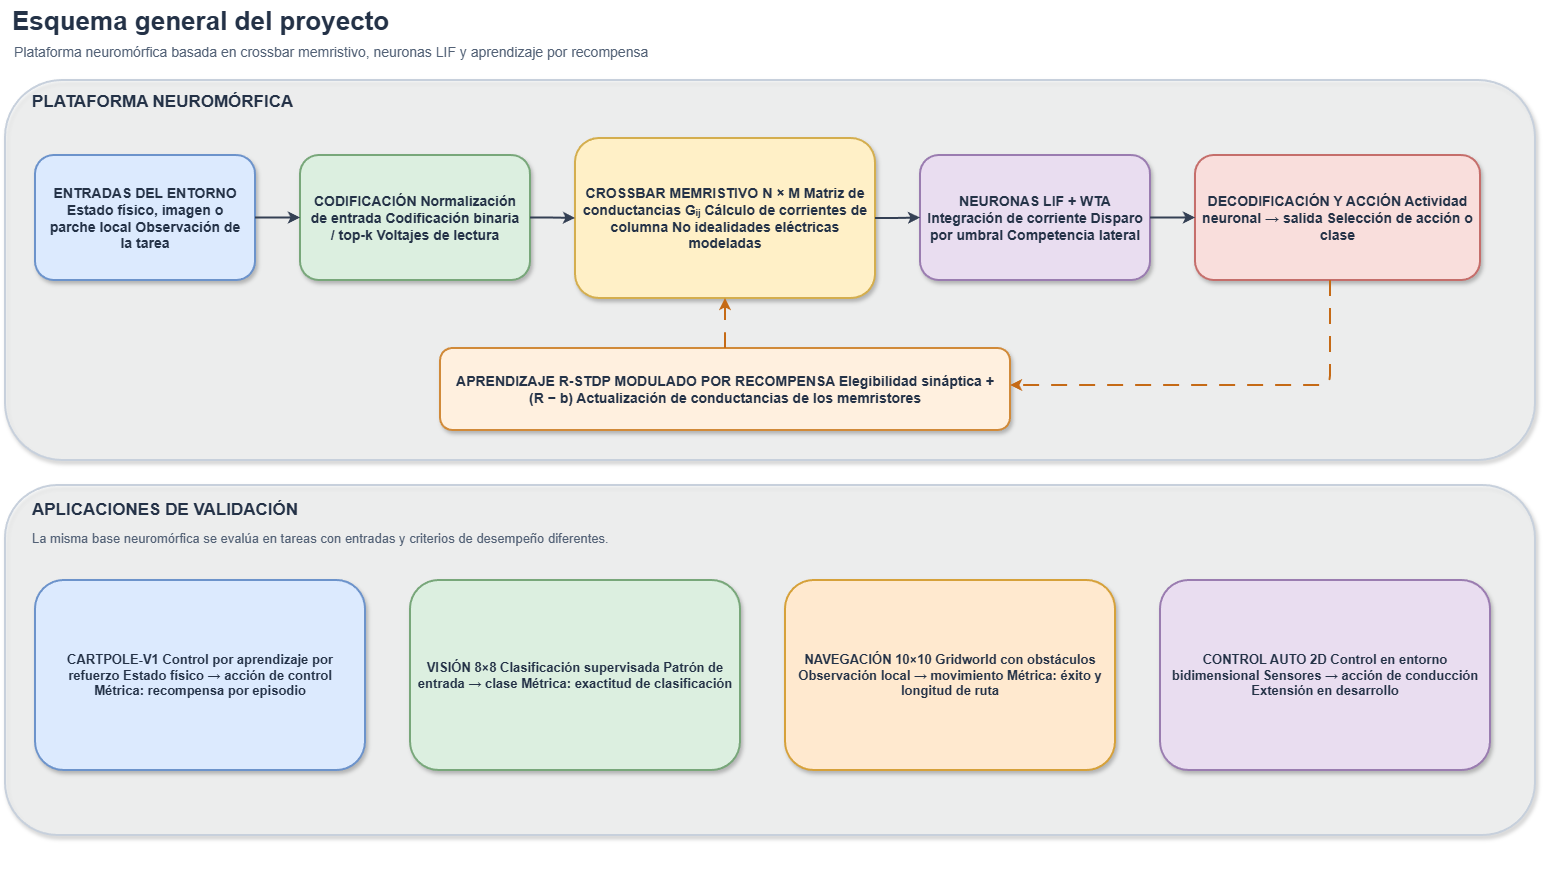
\includegraphics[width=0.86\textwidth]{figuras/esquema_general.png}
\caption[Arquitectura general del ecosistema]{Arquitectura general del ecosistema. El laboratorio 
(\textit{arriba}) provee los modelos físicos; el simulador 
robótico (\textit{abajo}) los integra en un agente de control.}
\label{fig:esquema_general}
\end{figure}

El flujo de información del agente sigue la secuencia 
\textit{sensores} $\rightarrow$ \textit{codificador} 
$\rightarrow$ \textit{crossbar} $\rightarrow$ \textit{decodificador} 
$\rightarrow$ \textit{actuadores}, con el aprendizaje aplicado al 
final de cada episodio mediante una regla de plasticidad 
modulada por recompensa. El detalle de cada componente se 
desarrolla en la Sección~\ref{sec:desarrollo}.

% =====================================================
\section{Herramientas}

El proyecto se desarrolló con herramientas de código abierto,
sin dependencias de software propietario. La Tabla~\ref{tab:hardware} y la
Tabla~\ref{tab:software} listan los componentes principales utilizados.

\subsection{Hardware}

\begin{table}[H]
\centering
\caption{Herramientas de hardware utilizadas.}
\label{tab:hardware}
\begin{tabular}{lp{9cm}}
\hline
\textbf{Componente} & \textbf{Uso} \\
\hline
Laptop de desarrollo & Ejecución de simulaciones y scripts Python (CPU x86-64, 8 GB RAM, SSD) \\
\hline
\end{tabular}
\end{table}

\subsection{Software}

\begin{table}[H]
\centering
\caption{Herramientas de software utilizadas.}
\label{tab:software}
\begin{tabular}{lp{9cm}}
\hline
\textbf{Herramienta} & \textbf{Uso} \\
\hline
Python 3.10+ & Lenguaje principal del simulador \\
NumPy & Álgebra lineal y matrices del crossbar \\
Matplotlib & Generación de figuras y visualización \\
PySide6 & Interfaces gráficas del laboratorio neuromórfico \\
Tkinter & Diálogos de configuración de las aplicaciones \\
Git & Control de versiones \\
\hline
\end{tabular}
\end{table}

% =====================================================

% =====================================================
\section{Metodolog\'ia del agente neurom\'orfico}
\label{sec:metodologia_agente}
\label{sec:desarrollo}

El agente recibe el estado del entorno, lo codifica en entradas del crossbar,
lee sus corrientes de columna y convierte la salida neuronal en una acci\'on.
El arreglo constituye el sustrato de pesos; el entorno y la recompensa se
simulan en software. El desarrollo detallado de los dispositivos, la LIF,
la plasticidad y el solver se documenta en el Ap\'endice~\ref{ap:desarrollo_extendido}.

\subsection{Configuraci\'on de referencia}

CartPole usa un crossbar de $24\times12$, lectura a $0.05\,\mathrm{V}$ y
una neurona LIF por salida. El estado normalizado $X$ se convierte en
resistencia mediante $R(X)=R_{\mathrm{on}}+X(R_{\mathrm{off}}-R_{\mathrm{on}})$;
por ello, $X$ es un estado interno del modelo y no una conductancia. La
configuraci\'on nominal es $R_{\mathrm{on}}=100\,\Omega$,
$R_{\mathrm{off}}=16\,\mathrm{k}\Omega$, $X_0=0.1$ y l\'imites
$0\leq X\leq1$. La tabla resume los par\'ametros el\'ectricos y temporales
usados como referencia.

\begin{table}[H]
\centering
\small
\caption{Par\'ametros de referencia del agente CartPole.}
\label{tab:parametros_agente}
\begin{tabular}{lll}
\toprule
Par\'ametro & Configuraci\'on & Valor efectivo\\
\midrule
$R_{\mathrm{on}}$ & $100\,\Omega$ & $100\,\Omega$\\
$R_{\mathrm{off}}$ & $16\,\mathrm{k}\Omega$ & $16\,000\,\Omega$\\
Estado inicial & $X_0=0.1$ & $x_0=0.9$ bajo $X=1-x$\\
$V_{\mathrm{read}}$ & $0.05\,\mathrm{V}$ & $0.05\,\mathrm{V}$\\
$V_{\mathrm{th}}$ LIF & $1.0\,\mathrm{V}$ & $1.0\,\mathrm{V}$\\
$t_{\mathrm{ref}}$ & $2\,\mathrm{ms}$ & $2\times10^{-3}\,\mathrm{s}$\\
$dt$ & -- & $10^{-4}\,\mathrm{s}$\\
\bottomrule
\end{tabular}
\end{table}

En CartPole, las observaciones se codifican en filas activas; el solver
nodal MNA calcula las corrientes considerando la conductancia del crossbar
y las resistencias configuradas de l\'inea y sensado. Las neuronas LIF
integran las corrientes, generan spikes al alcanzar el umbral y se reinician
seg\'un el per\'iodo refractario. La decisi\'on de acci\'on se obtiene de la
actividad de salida. Estos pasos describen el simulador, no un circuito
fabricado.

La lectura del agente calcula $G(X)$ y resuelve la red MNA sin integrar la
dinamica no volatil del estado durante ese paso; el metodo de lectura no
llama a la actualizacion de las celdas, por lo que en esta ruta simulada
$\Delta X=0$ por construccion. Esto cuantifica el cambio de estado impuesto
por el software en cada lectura, no una perturbacion electrica medida en un
dispositivo fisico. El modelo Strukov del laboratorio si incorpora un
umbral de deriva ionica de $0.1\,\mathrm{V}$ como valor predeterminado
de \texttt{StrukovConfig}; ese umbral se aplica al integrar la dinamica de la celda y no es una medicion
experimental del umbral del dispositivo. El dispositivo volatil de salida,
en cambio, si se actualiza en cada paso y modula la corriente que recibe
la LIF.

\subsection{Reglas de aprendizaje y decisi\'on}

En REINFORCE, el agente conserva una elegibilidad por conexi\'on durante el
episodio y la actualiza al terminarlo seg\'un el retorno y un baseline. La
contribuci\'on instant\'anea es
\[
e_{ij,t}=\mathrm{pre}_{i,t}
\left(\mathbf{1}_{j=\mathrm{col}_t}-\pi_{j,t}\right),\qquad
E_{ij,t}=\gamma E_{ij,t-1}+e_{ij,t},
\]
donde $\pi_{j,t}$ es la probabilidad softmax de la columna $j$. La softmax
convierte puntuaciones en probabilidades que suman uno: una temperatura alta
reparte m\'as la probabilidad y una baja la concentra. El decoder muestrea
seg\'un esa distribuci\'on y la regla de aprendizaje ajusta el crossbar con el
resultado del episodio. Esta forma de gradiente de pol\'itica se basa en REINFORCE y en los m\'etodos
de aprendizaje por refuerzo descritos en la literatura~\cite{Williams1992REINFORCE,SuttonBarto2018}. La implementaci\'on se describe en
\url{robot_sim/neurobot/reinforce_agent.py} y
\url{robot_sim/neurobot/crossbar_brain.py}.

La regla local STDP del laboratorio usa spikes binarios pre/post y trazas
exponenciales $p_i$ y $q_j$:
\[
\tau_{\mathrm{pre}}\dot p_i=-p_i+s_i^{\mathrm{pre}},\qquad
\tau_{\mathrm{post}}\dot q_j=-q_j+s_j^{\mathrm{post}},\qquad
\Delta G_{ij}^{\mathrm{STDP}}=\eta\left(A_+p_i s_j^{\mathrm{post}}
-A_-s_i^{\mathrm{pre}}q_j\right).
\]
En la regla R-STDP del m\'odulo, la elegibilidad decae y acumula ese cambio:
\[
E_{ij,t}=e^{-dt/\tau_e}E_{ij,t-1}+\Delta G_{ij,t}^{\mathrm{STDP}},
\qquad \Delta G_{ij,t}^{\mathrm{R-STDP}}=R_tE_{ij,t}.
\]
Esta formulaci\'on de elegibilidad modulada por recompensa sigue el marco
conceptual de R-STDP~\cite{Izhikevich2007RSTD}; en este proyecto, la regla
local implementada se describe en \url{neurolab/crossbar/plasticity.py}.

Las corridas del agente etiquetadas R-STDP en el Ap\'endice
\ref{ap:evidencia_entrenamientos} no implementan esa regla estricta con
spikes LIF como evento post. En los entornos de control, el runner construye
un evento de acci\'on centrado por la pol\'itica,
$z_{j,t}=\mathbf{1}_{j=a_t}-\pi_{j,t}$, y una elegibilidad por decisi\'on
$e_{ij,t}=a_+\,\mathrm{pre}_{i,t}\max(z_{j,t},0)
+a_-\,\mathrm{pre}_{i,t}\min(z_{j,t},0)$. Los spikes LIF y los ganadores
WTA se registran, pero no sustituyen a $z_{j,t}$ en esta actualizaci\'on;
la tarea de visi\'on usa una elegibilidad derivada del gradiente de corriente.
Para cada paso se calcula el retorno descontado $G_t=r_t+\gamma G_{t+1}$,
la ventaja $A_t=G_t-b_t$ respecto al baseline temporal previo y su
normalizaci\'on $\widehat A_t=A_t/s_A$, donde
$s_A=\max(\operatorname{std}(A),10^{-8})$ (se usa $s_A=1$ para un solo
paso). La elegibilidad modulada del episodio es
\[
E^R_{ij}=\frac{1}{\sqrt{T}}\sum_{t=0}^{T-1} e_{ij,t}\widehat A_t,
\qquad \Delta X=-\eta E^R.
\]
El cambio se escala para cumplir el l\'imite configurado de
$\max_{ij}|\Delta X_{ij}|$ y se anula en episodios que alcanzan el umbral
de congelamiento. La actualizaci\'on opera directamente sobre el estado
abstracto $X$ y las variabilidades D2D/C2C modifican el incremento aplicado.
Para $E^R>0$, $\Delta X<0$ reduce $R(X)$ y aumenta $G(X)$; el signo opuesto
produce el efecto contrario. Esta comprobaci\'on algebraica confirma la
direcci\'on del mapeo en el c\'odigo, pero no demuestra aprendizaje estable
ni programaci\'on por pulsos f\'isicos. Por ello, en
esta tesis las corridas del runner se describen como el piloto h\'ibrido
pre/acci\'on modulado por retorno (conservando R-STDP como nombre del modo
del software), no como evidencia de R-STDP can\'onica pre/post. La variante
de tarea que s\'i emple\'o spikes LIF reales como evento post tuvo bajo
rendimiento exploratorio. Los resultados y su alcance se informan en la
Secci\'on~\ref{sec:piloto_rstdp_reinforce}; la topolog\'ia y el modelo
el\'ectrico del crossbar se mantienen entre reglas de aprendizaje.

\subsection{Aplicaciones evaluadas}

La misma organizaci\'on se adapt\'o a cuatro tareas. Se conservaron la lectura
del crossbar y la actualizaci\'on por recompensa; las dimensiones y el
significado de la salida dependen del entorno. Los registros por condici\'on
se incluyen en el Ap\'endice~\ref{ap:evidencia_entrenamientos}.

\begin{table}[H]
\centering
\small
\caption{Configuraci\'on de las aplicaciones simuladas.}
\label{tab:aplicaciones}
\begin{tabularx}{\textwidth}{l c X X}
\toprule
Tarea & Crossbar & Entrada y salida & M\'etrica\\
\midrule
CartPole & $24\times12$ & Estado continuo; dos acciones & Recompensa y supervivencia\\
Visi\'on & $64\times8$ & Patr\'on binario $8\times8$; ocho clases & Exactitud\\
Obst\'aculos & $16\times4$ & Sensores del gridworld; cuatro movimientos & Llegada a meta\\
Auto 2D & $24\times8$ & Rayos, direcci\'on y distancia; cuatro controles & Llegada a meta\\
\bottomrule
\end{tabularx}
\end{table}

\section{Validaci\'on de modelos}
\label{sec:validacion_modelos}

La validaci\'on se organiz\'o en tres niveles: comprobaciones internas de
c\'odigo y unidades, comparaci\'on de series simuladas con puntos digitalizados
de publicaciones y pruebas funcionales de las aplicaciones. Solo se
presentan m\'etricas cuando existe correspondencia punto a punto y protocolo
definido. Una coincidencia visual, una distribuci\'on sint\'etica o una traza
producida por el mismo modelo no equivalen a una medici\'on de hardware. El
inventario de fuentes y scripts est\'a en el ap\'endice de datos; los protocolos
completos se conservan en el Ap\'endice~\ref{ap:desarrollo_extendido}.

\begin{figure}[H]
\centering
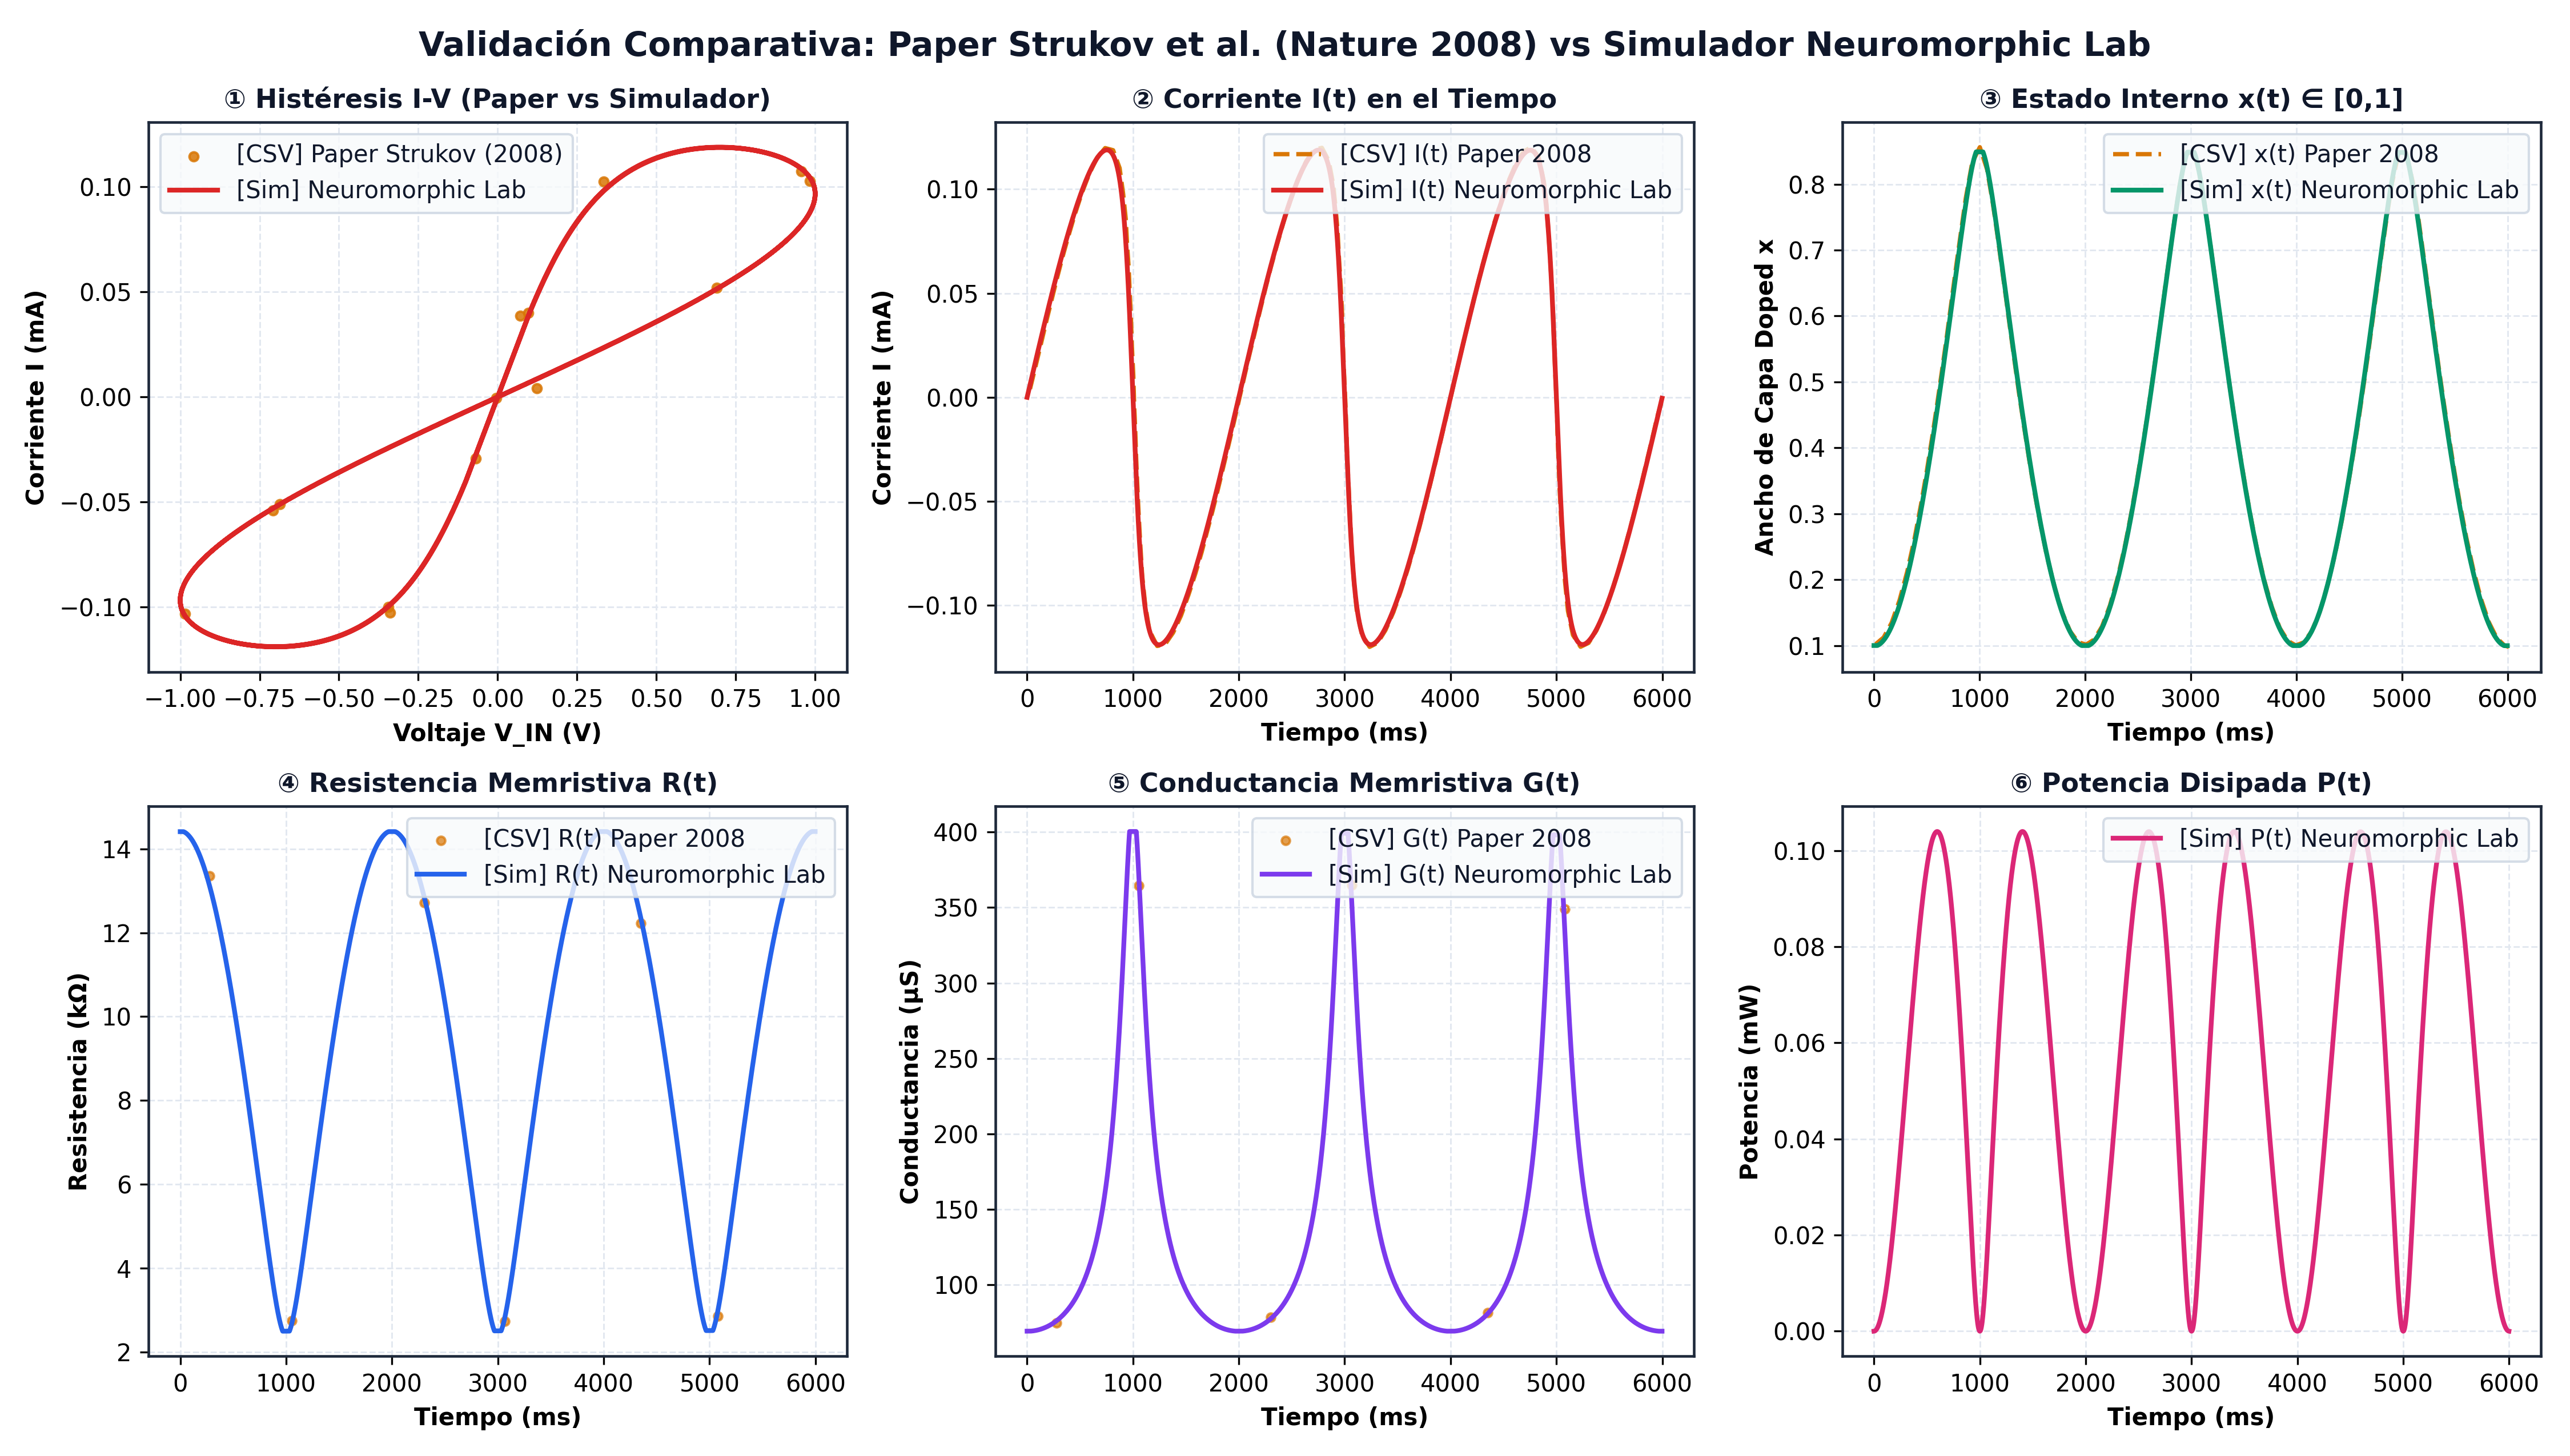
\includegraphics[width=0.78\textwidth]{figuras/fig_01_strukov.png}
\caption{Curvas del modelo Strukov local comparadas con las series digitalizadas atribuidas a la referencia.}
\label{fig:strukov_iv}
\end{figure}

\subsection{Comparaciones cuantitativas}

Para Strukov se compararon estado, corriente, resistencia y conductancia
con series digitalizadas atribuidas al art\'iculo de 2008. Prezioso es una
comparaci\'on visual, pues los puntos no contienen protocolo temporal
completo. La ventana STDP usa nueve puntos de ajuste y cuatro reservados;
LTP/LTD usa 18 puntos de test. La LIF $f-I$ compara Euler con la soluci\'on
anal\'itica del mismo modelo, no con mediciones experimentales. La tabla
resume las m\'etricas reproducibles.

\begin{table}[H]
\centering
\footnotesize
\caption{M\'etricas de validaci\'on reproducibles. $R^2$ es el coeficiente de determinaci\'on; ERP se normaliza por el rango de referencia.}
\label{tab:metricas_validacion}
\begin{tabularx}{\textwidth}{X c c c c c}
\toprule
Comparaci\'on & $n$ & $R^2$ & MAE & RMSE & ERP (\%)\\
\midrule
Strukov, estado $x(t)$ &107&0.999657&0.003676&0.004491&1.27\\
Strukov, corriente $I(t)$ &136&0.996994&0.002586 mA&0.004126 mA&6.22\\
Strukov, resistencia $R(t)$ &87&0.998319&0.135431 k$\Omega$&0.162264 k$\Omega$&3.54\\
Strukov, conductancia $G(t)$ &87&0.983726&7.55759 $\mu$S&15.64415 $\mu$S&19.04\\
Prezioso, $I(V)$ visual &179&--&--&--&--\\
STDP, holdout &4&0.94220&1.90404 pp&2.13626 pp&14.87\\
LTP/LTD, test &18&0.73988&8.3491 nA&8.6181 nA&31.23\\
LIF $f-I$, Euler vs anal\'itica &14&0.999964&0.086431 Hz&0.151393 Hz&0.55\\
\bottomrule
\end{tabularx}
\end{table}

STDP y LTP/LTD proceden de conjuntos digitalizados peque\~nos; sus par\'ametros
ajustados son efectivos y no caracterizan independientemente un dispositivo.
En LTP/LTD, el resultado agregado oculta un ajuste deficiente por rama.
Prezioso carece de etiquetas temporales y de rama suficientes para una
m\'etrica. La prueba D2D/C2C verifica propiedades estad\'isticas de muestras
sint\'eticas, no una poblaci\'on experimental. Las Figuras
\ref{fig:stdp_curve_ch3} y \ref{fig:ltp_ltd_curve_ch3} permiten inspeccionar
los datos atribuidos a Jo et al.; las particiones y limitaciones se ampl\'ian
en el ap\'endice t\'ecnico.

\begin{table}[H]
\centering
\footnotesize
\caption{Cumplimiento de los umbrales cuantitativos cuando son aplicables.}
\label{tab:estado_criterios_modelos}
\begin{tabularx}{\textwidth}{l c c X}
\toprule
Prueba & ERP $<10\%$ & $R^2>0.90$ & Conclusi\'on\\
\midrule
Strukov: $x$, $I$, $R$ & S\'i & S\'i & Cumplen en las series comparadas.\\
Strukov: $G$ & No & S\'i & ERP $=19.04\%$; no cumple todos los umbrales.\\
STDP, holdout ($n=4$) & No & S\'i & Parcial; ERP $=14.87\%$ y muestra peque\~na.\\
LTP/LTD ($n=18$) & No & No & No cumple; $R^2=0.73988$, ERP $=31.23\%$.\\
Prezioso $I(V)$ & No calculable & No calculable & Comparaci\'on visual; faltan puntos con protocolo suficiente.\\
LIF $f-I$ & S\'i$^*$ & S\'i$^*$ & Verificaci\'on interna frente a soluci\'on anal\'itica, no validaci\'on experimental independiente.\\
\bottomrule
\end{tabularx}
\par\smallskip\scriptsize $^*$M\'etricas de integraci\'on para el mismo modelo anal\'itico; no se interpretan como concordancia con hardware publicado.
\end{table}

\begin{figure}[H]
\centering
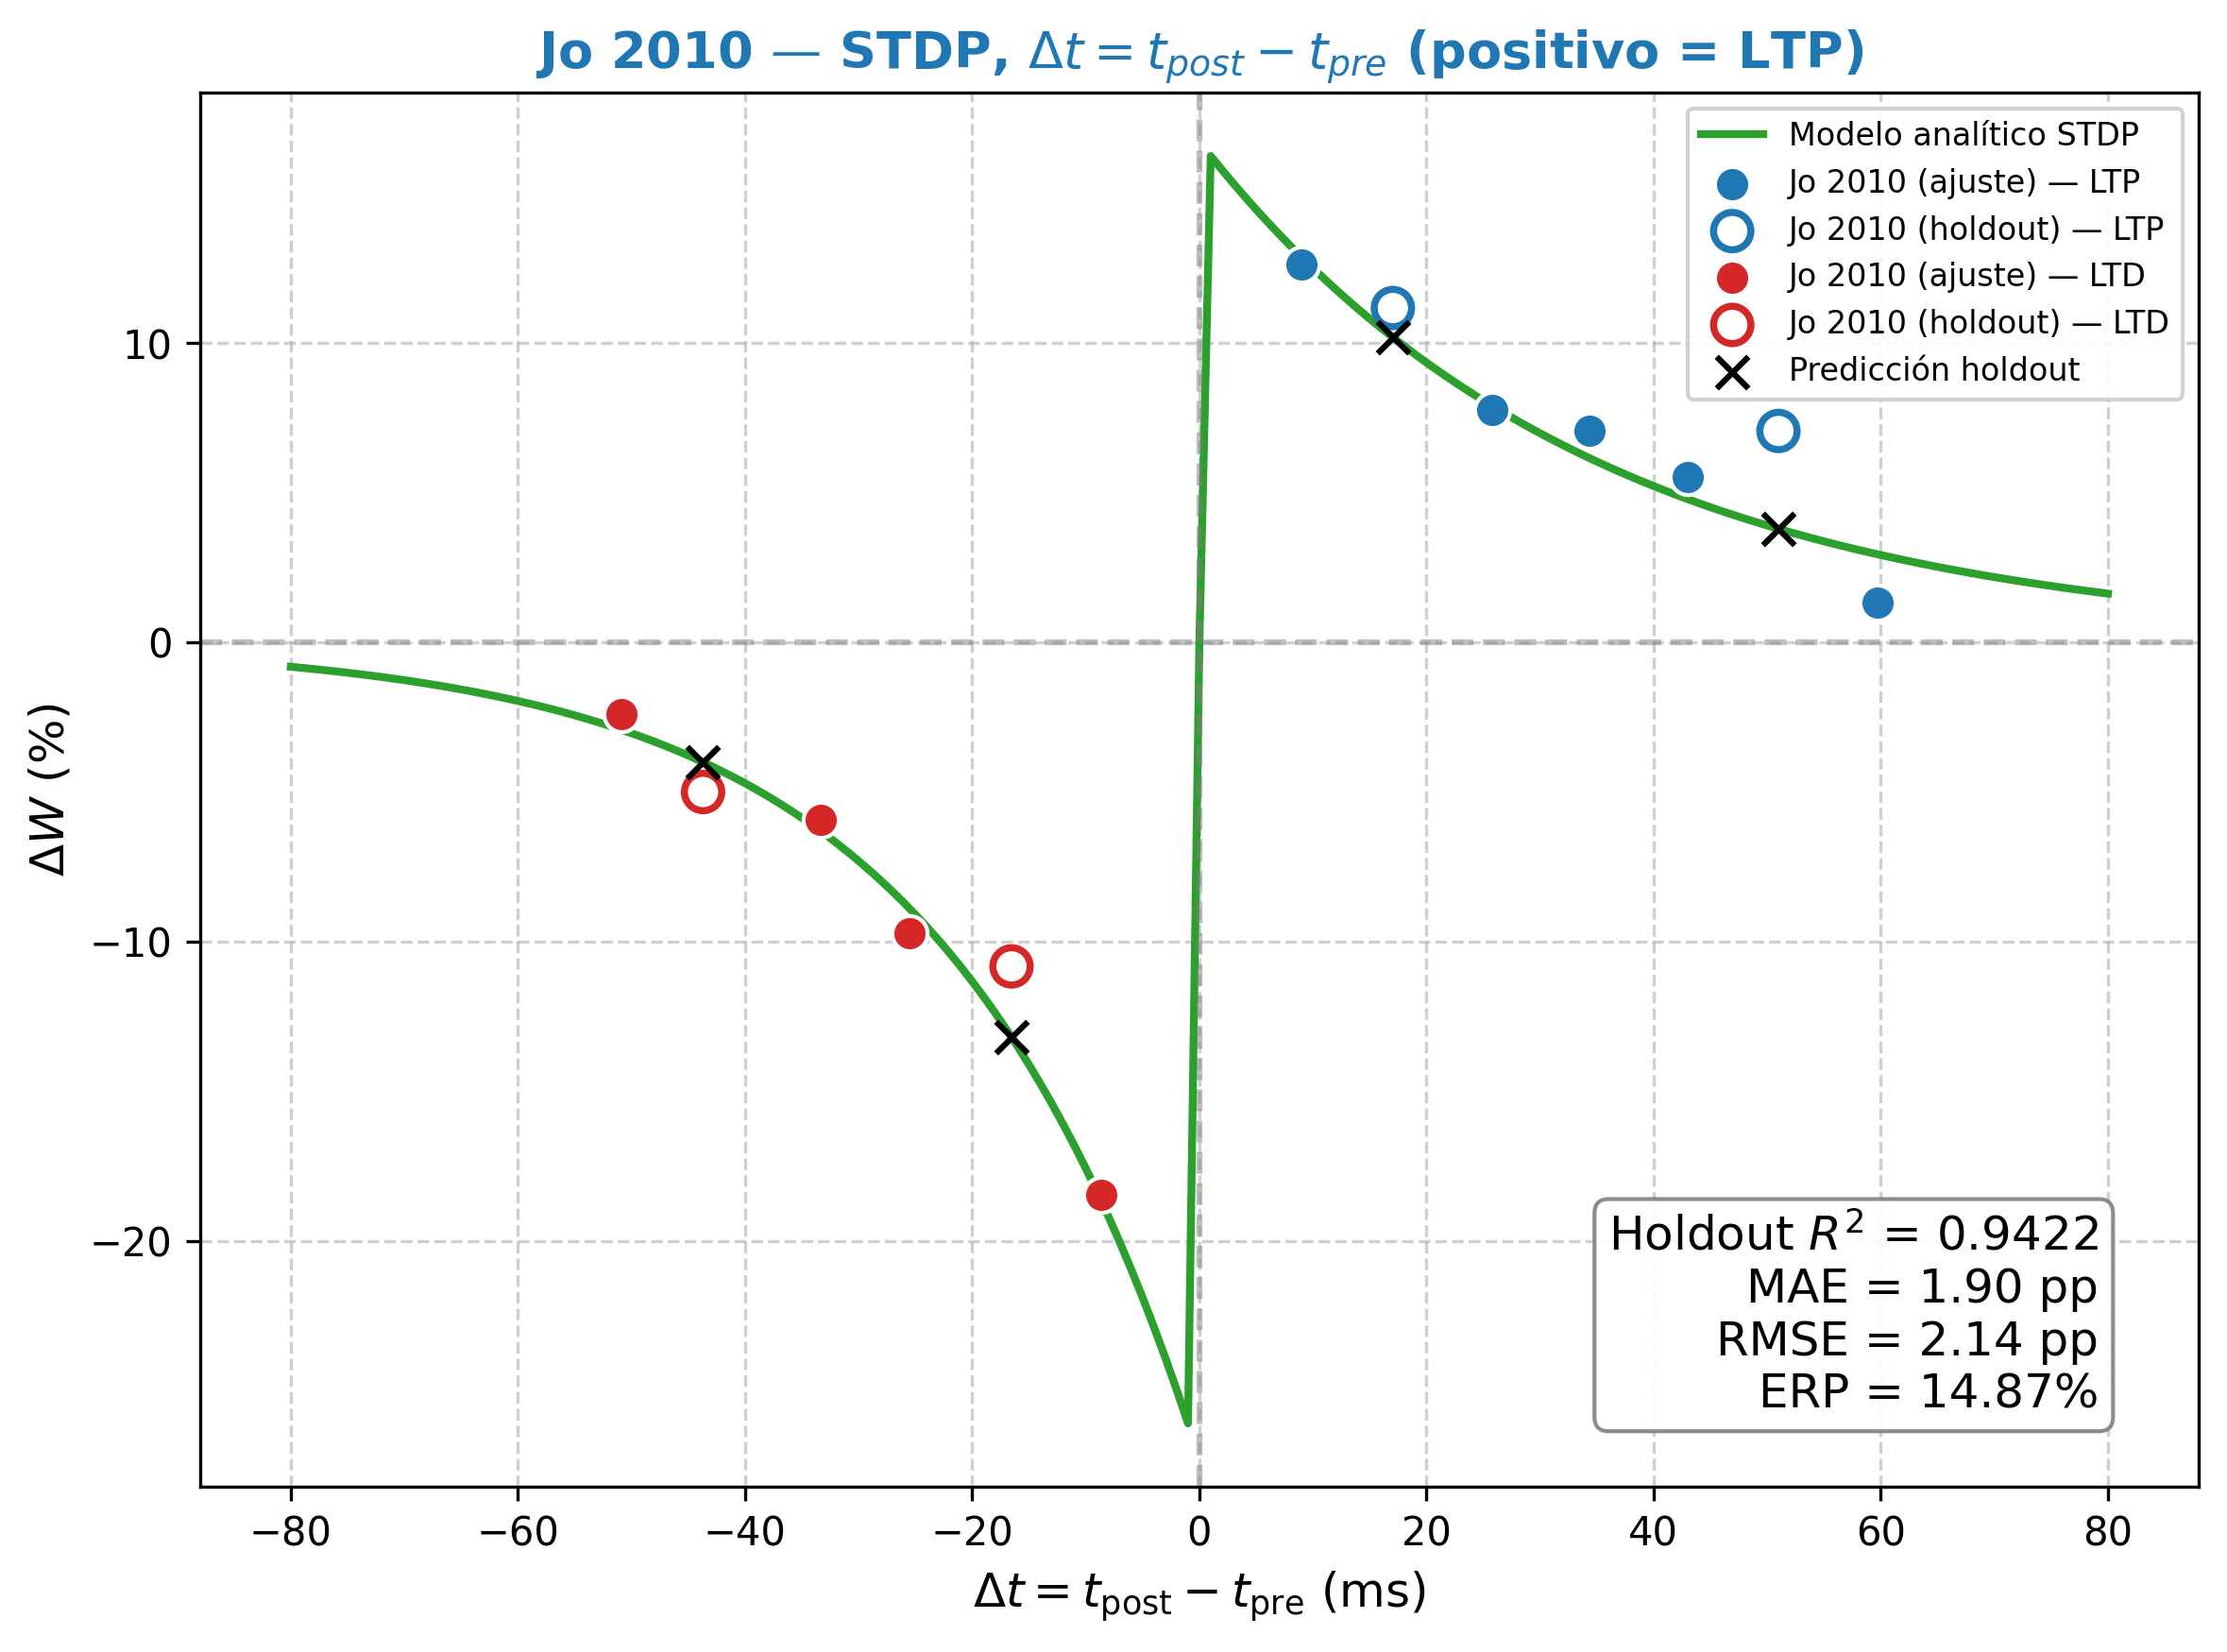
\includegraphics[width=0.72\textwidth]{figuras/fig_15b_stdp_jo2010.png}
\caption{Ajuste STDP en nueve puntos y evaluaci\'on en cuatro puntos reservados atribuidos a Jo et al. (2010).}
\label{fig:stdp_curve_ch3}
\end{figure}
\begin{figure}[H]
\centering
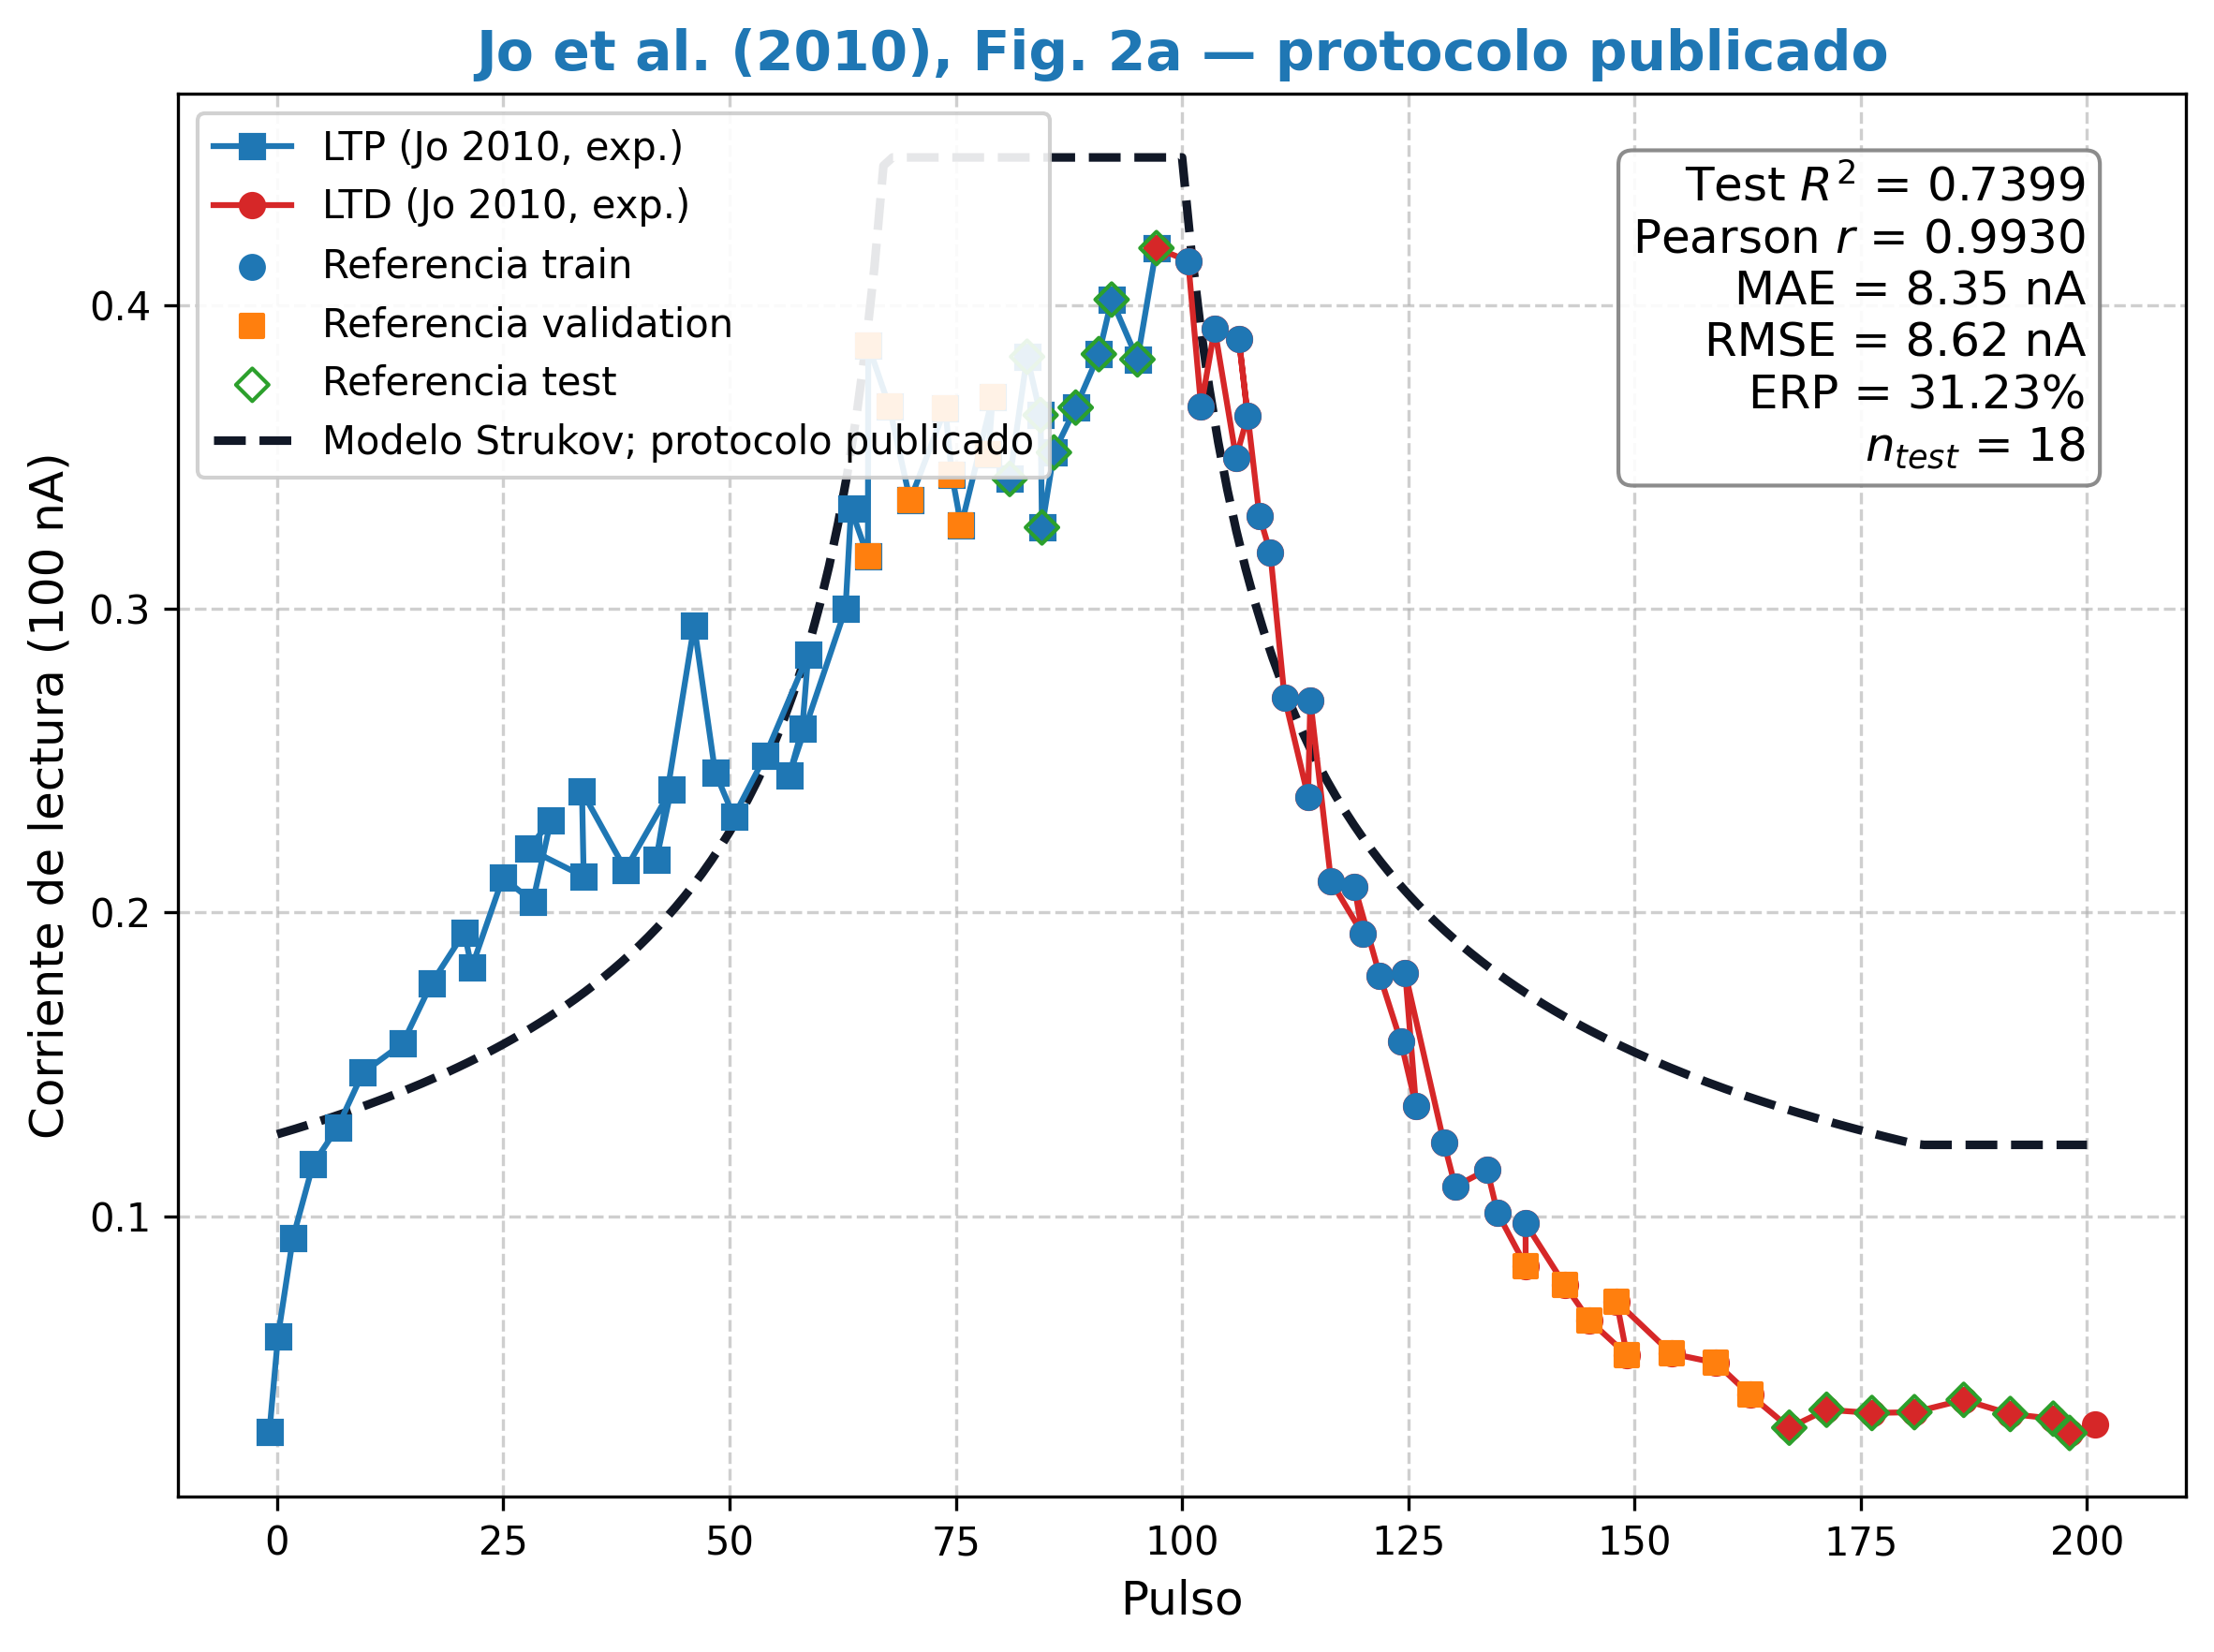
\includegraphics[width=0.72\textwidth]{figuras/fig_14b_ltp_ltd_jo2010.png}
\caption{Comparaci\'on LTP/LTD atribuida a Jo et al. (2010); los par\'ametros se ajustaron con datos de entrenamiento.}
\label{fig:ltp_ltd_curve_ch3}
\end{figure}

\begin{table}[H]
\centering
\small
\caption{Cumplimiento de objetivos seg\'un el alcance de la evidencia.}
\label{tab:cumplimiento_objetivos}
\begin{tabularx}{\textwidth}{l X l}
\toprule
Objetivo & Evidencia resumida & Estado\\
\midrule
Modelos memristivos y variabilidad & Comparaciones digitalizadas y pruebas sint\'eticas; alcance acotado. & Parcial\\
Neurona LIF & Disparo, reinicio, refractario y curva $f-I$ frente a soluci\'on anal\'itica. & Verificado internamente\\
Plasticidad local & STDP con cuatro puntos reservados; conjunto peque\~no. & Parcial\\
Crossbar & Solver MNA y comprobaci\'on num\'erica; sin medici\'on f\'isica. & Verificado en simulaci\'on\\
Aprendizaje de tareas & REINFORCE de referencia y piloto R-STDP con resultados variables. & Parcial\\
\bottomrule
\end{tabularx}
\end{table}

\subsection{Verificaci\'on del sistema integrado}
\label{sec:crossbar_manual}

Se verific\'o la conversi\'on de unidades, un caso manual de crossbar $2\times2$
y la invariancia de pesos durante evaluaciones congeladas. La respuesta LIF
se contrast\'o con la soluci\'on anal\'itica frecuencia--corriente; la prueba
temporal comprueba umbral, reinicio y refractario en el propio modelo. El
Ap\'endice t\'ecnico distingue estas verificaciones de una validaci\'on f\'isica.

La prueba manual usa $G=[[0.001,0.0005],[0.00033333,0.00025]]\,\mathrm{S}$ y
$V=[0.05,0]^{\mathsf T}\,\mathrm{V}$. La multiplicaci\'on ideal produce
$[50,25]~\mu\mathrm{A}$; el solver MNA produce $[44.1176,23.2558]~\mu\mathrm{A}$.
La diferencia corresponde a las resistencias del protocolo del solver, no a
la identidad matricial ideal.

\begin{figure}[H]
\centering
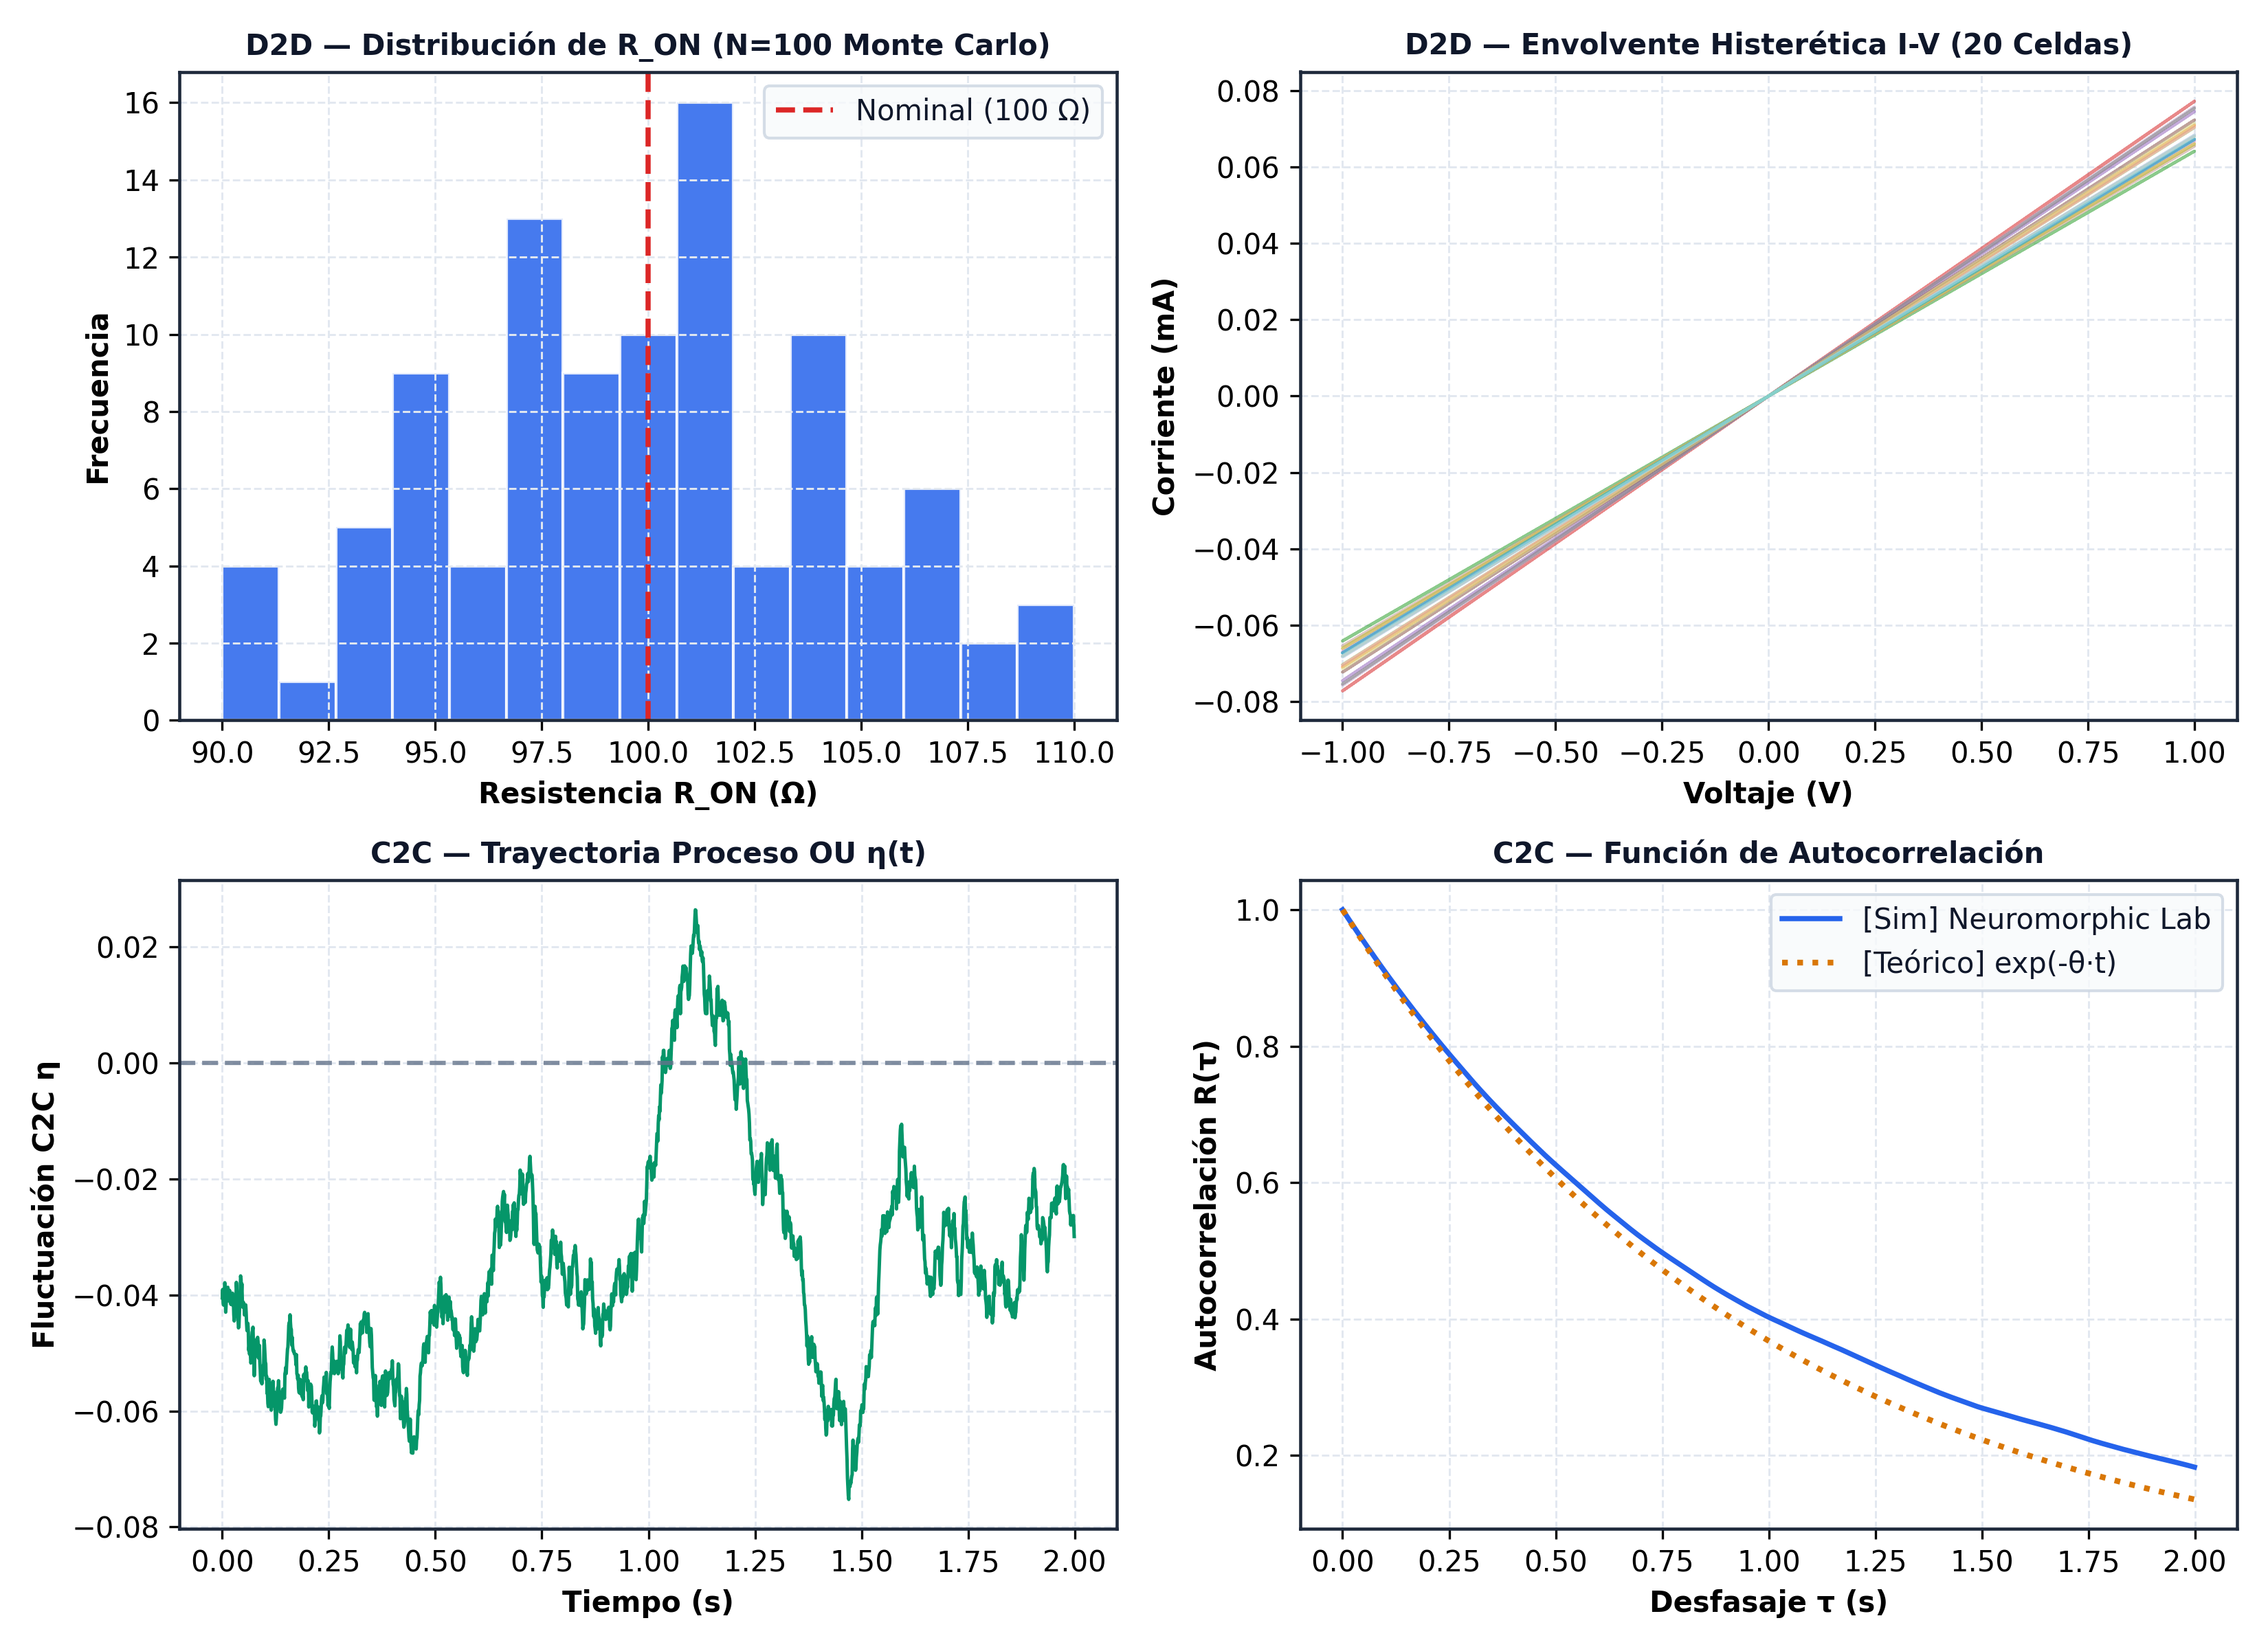
\includegraphics[width=0.67\textwidth]{figuras/fig_05_d2d_c2c.png}
\caption{Distribuciones sint\'eticas D2D/C2C del modelo y sus referencias te\'oricas; no son histogramas de mediciones f\'isicas.}
\label{fig:d2d_c2c_validation}
\end{figure}

\begin{figure}[H]
\centering
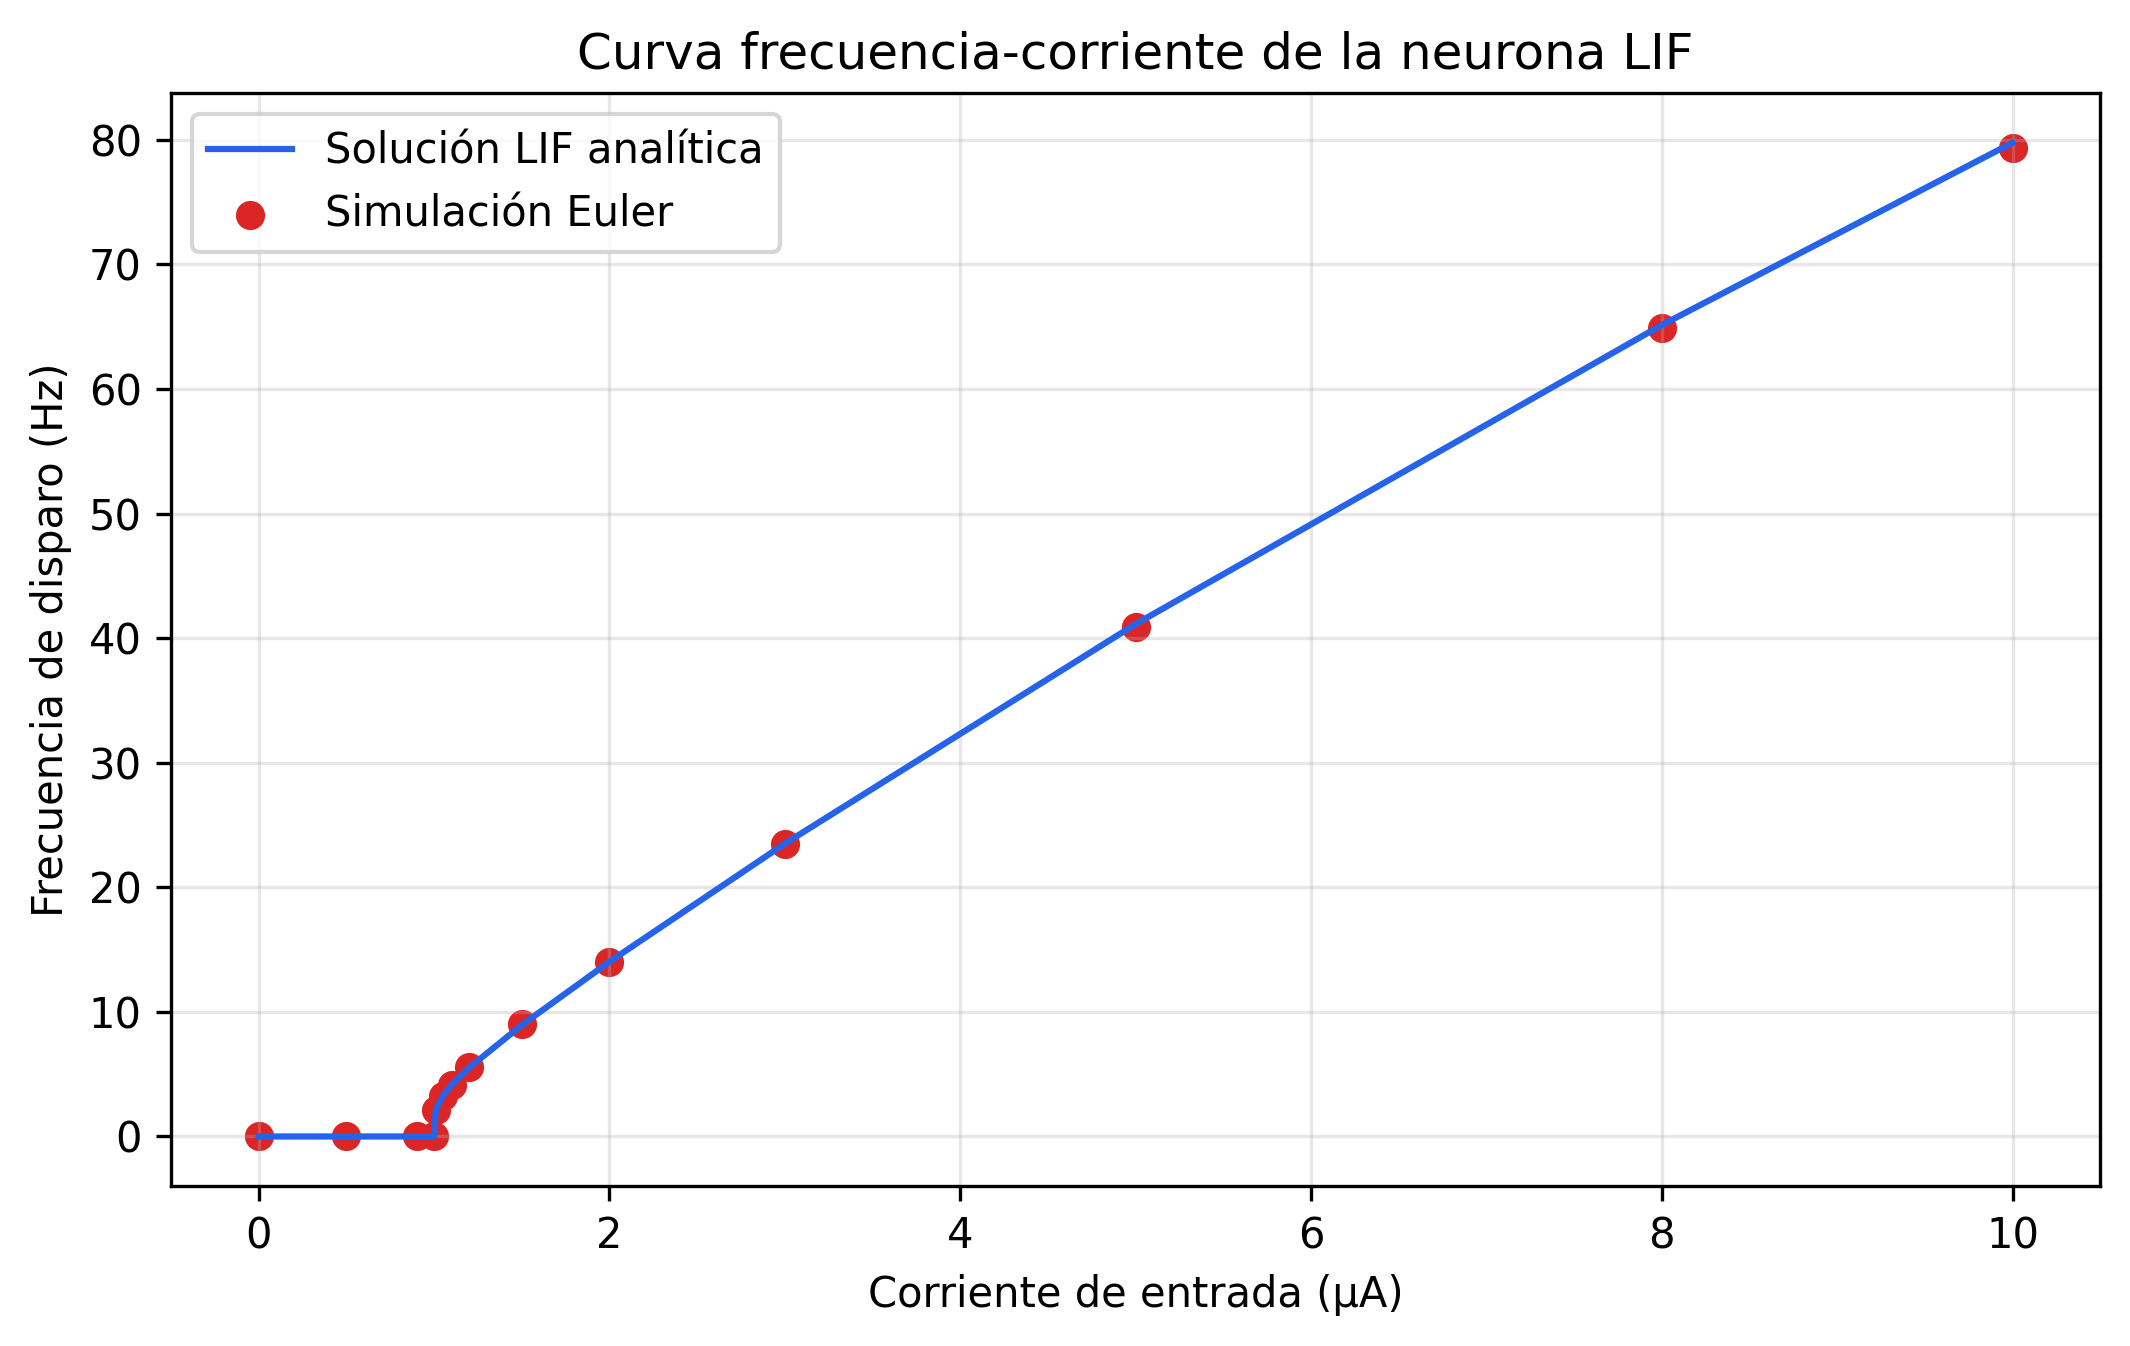
\includegraphics[width=0.67\textwidth]{figuras/lif_fi_curve.png}
\caption{Frecuencia de disparo LIF por Euler frente a la soluci\'on anal\'itica del mismo modelo.}
\label{fig:lif_fi_curve}
\end{figure}

\section{Resultados y discusi\'on}
\label{sec:resultados}

Las m\'etricas de cada aplicaci\'on son espec\'ificas y no se interpretan como
comparaci\'on controlada cuando cambian la arquitectura, la recompensa o el
presupuesto de entrenamiento. Los registros y matrices por condici\'on est\'an
en el Ap\'endice~\ref{ap:evidencia_entrenamientos}.


\begin{table}[H]
\centering
\scriptsize
\setlength{\tabcolsep}{3pt}
\caption{Separaci\'on de entrenamiento, validaci\'on y test en las aplicaciones.}
\label{tab:train_validation_test_tasks}
\begin{tabularx}{\textwidth}{l X X X}
\toprule
Tarea & Entrenamiento & Validaci\'on y selecci\'on & Test independiente\\
\midrule
CartPole & Cinco semillas, 300 episodios cada una. & 50 episodios por checkpoint; se selecciona semilla 4 ($493.77$). & 50 episodios, semillas 20000--20049; $493.63\pm0.93$.\\
Visi\'on & Tres semillas, 5000 episodios sobre ocho plantillas. & 160 variantes por checkpoint con inversi\'on de p\'ixel $p=0.05$; selecci\'on: semilla 2 ($42.5\%$). & 400 variantes nuevas; exactitud $42.5\%$.\\
Obst\'aculos & Semillas 0--2; 746, 800 y 800 episodios. & 20 mapas por checkpoint; selecci\'on: semilla 2 ($25\%$). & 50 mapas nuevos; \'exito $4\%$ (2/50).\\
Auto 2D & Una semilla; horizonte reportado de 3000 episodios y snapshots cada 200. & 20 escenarios por snapshot; checkpoint reportado con $15\%$. & 50 escenarios; \'exito reportado $14\%$ (7/50); faltan logs para recalcular.\\
\bottomrule
\end{tabularx}
\end{table}

\subsection{CartPole-v1: control con recompensa densa}
\label{sec:res_cartpole}

Se entren\'o el agente $24\times12$ durante 300 episodios en cinco semillas,
con D2D/C2C y supresi\'on de actualizaci\'on en cada episodio cuya recompensa
alcanz\'o 430. La recompensa media de los \'ultimos 200 episodios fue 369.66,
421.44, 474.31, 462.79 y 448.36 para las semillas 0--4 (media $435.31$,
desviaci\'on est\'andar $37.28$). Cuatro corridas alcanzaron una recompensa
epis\'odica de 480. El umbral omite una actualizaci\'on de pesos de ese episodio,
pero no congela permanentemente el agente.

Para evaluar dentro de la tarea, se seleccion\'o en validaci\'on el checkpoint
de la semilla 4 y se evalu\'o sin aprendizaje en 50 episodios de test
independientes. Obtuvo $493.63\pm0.93$ puntos (rango 490.43--494.94);
$X$ no cambi\'o y el decoder fue greedy. En la comparaci\'on emparejada
ideal--D2D/C2C, la diferencia media fue $+99.46\pm226.90$ puntos, pero
solo tres de cinco pares favorecieron la condici\'on variable; el resultado
es descriptivo y no prueba una ventaja general. La curva de cinco semillas
est\'a en la Figura~\ref{fig:cartpole_learning}.

\begin{figure}[H]
\centering
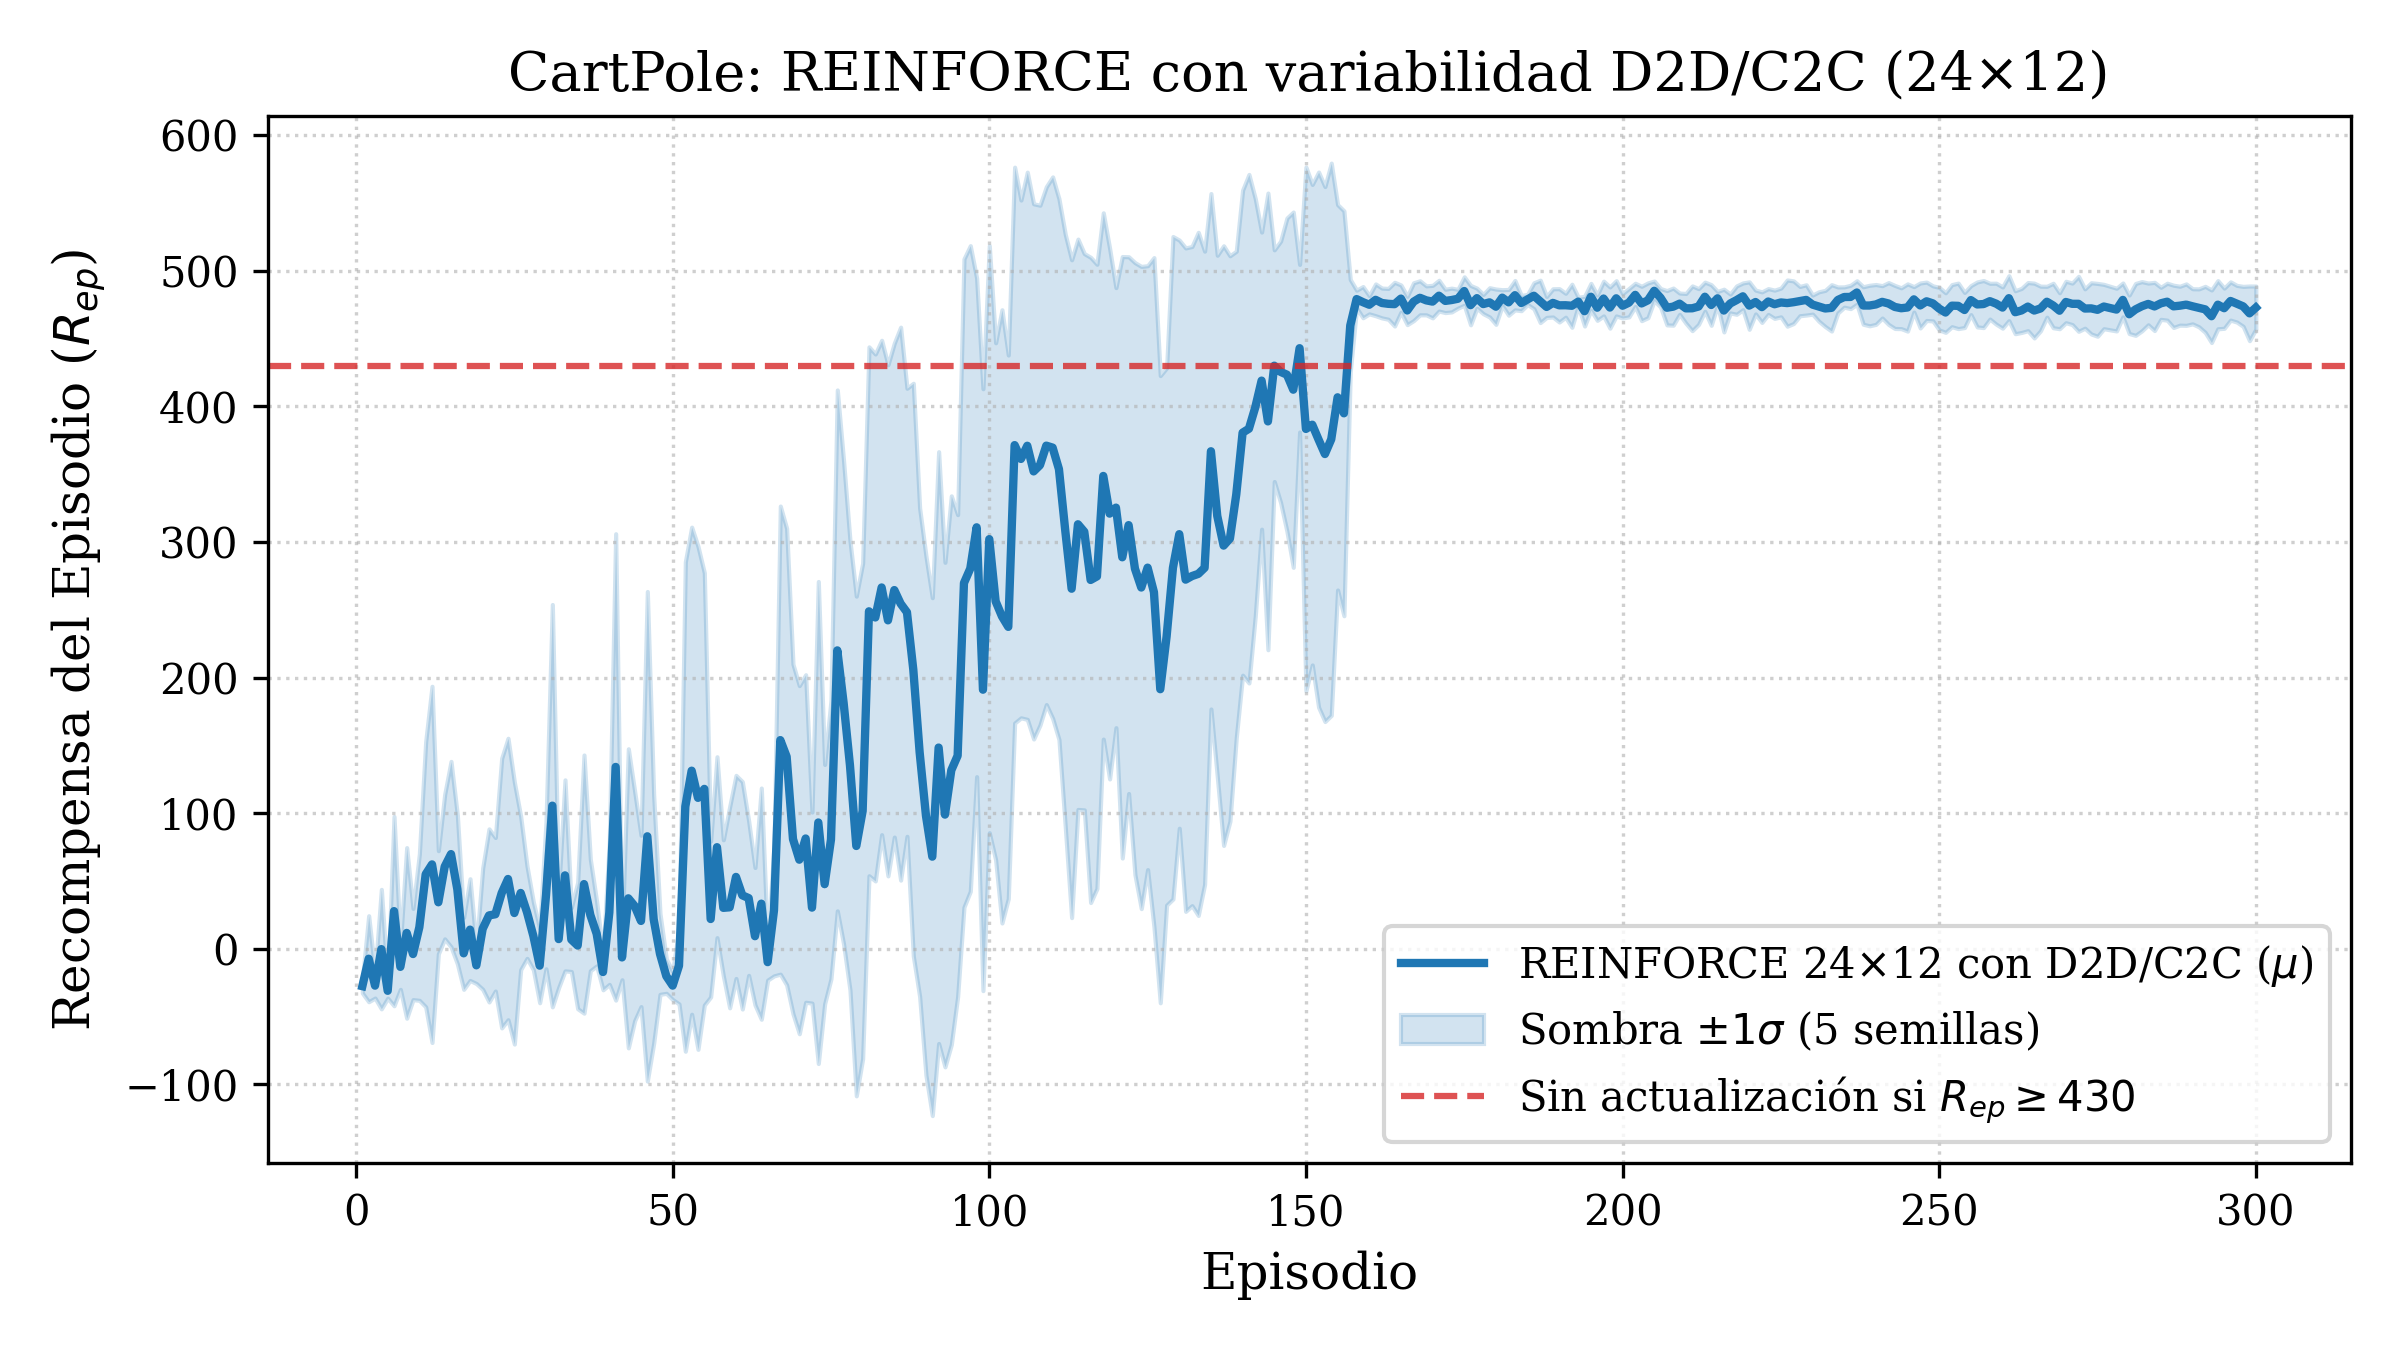
\includegraphics[width=0.76\textwidth]{figuras/cartpole_learning_24x12_5seeds_d2d_c2c.png}
\caption{Recompensa de cinco corridas CartPole con D2D/C2C, suavizada para facilitar la lectura.}
\label{fig:cartpole_learning}
\end{figure}

\subsection{Visi\'on $8\times8$: clasificaci\'on supervisada}
\label{sec:res_vision}

La tarea clasific\'o ocho patrones binarios mediante un crossbar $64\times8$.
En tres corridas de 5000 episodios, el acierto de los \'ultimos 200 episodios
fue 100\%. Ese dato corresponde a las ocho plantillas del entrenamiento.
Para medir robustez se reservaron variantes con inversi\'on de p\'ixeles; tras
selecci\'on por validaci\'on, la semilla 2 obtuvo 42.5\% sobre 400 variantes
de test, frente a 12.5\% aleatorio. El test mide ruido sint\'etico sobre las
plantillas, no clases ni im\'agenes externas.

\begin{figure}[H]
\centering
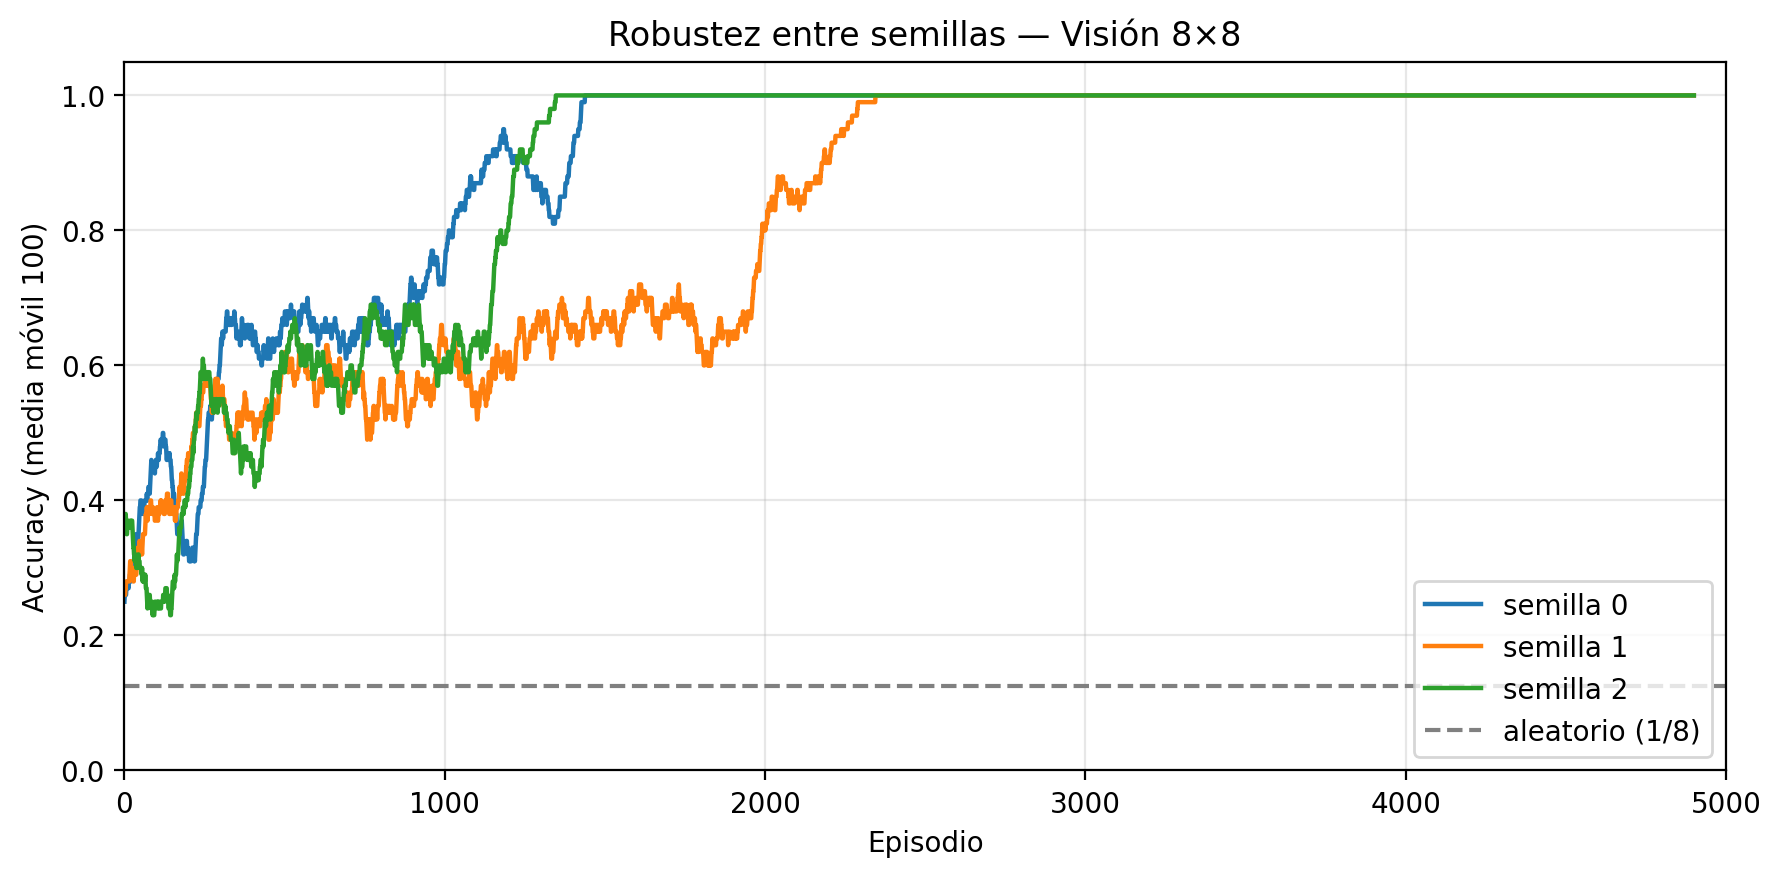
\includegraphics[width=0.72\textwidth]{figuras/vision_seeds.png}
\caption{Exactitud de tres corridas de visi\'on, suavizada con una ventana de 100 episodios.}
\label{fig:vision_seeds}
\end{figure}

\subsection{Navegaci\'on $10\times10$: control con recompensa escasa}
\label{sec:res_navegacion}

El gridworld contiene 15 obst\'aculos y cuatro movimientos, con recompensa
por llegar a la meta y penalizaciones por paso y colisi\'on. Las tasas de
\'exito de los \'ultimos 200 episodios fueron 100\%, 49.5\% y 82\% (media
no ponderada 77.17\%). En 50 mapas nuevos, el checkpoint seleccionado en
validaci\'on alcanz\'o la meta en 2 mapas (4\%). El buen resultado en el mapa
de entrenamiento no se transfiri\'o a mapas distintos en esta prueba. Los
registros de esa evaluaci\'on no est\'an incluidos como JSON recalculable y el
4\% se identifica como resultado reportado.

\begin{figure}[H]
\centering
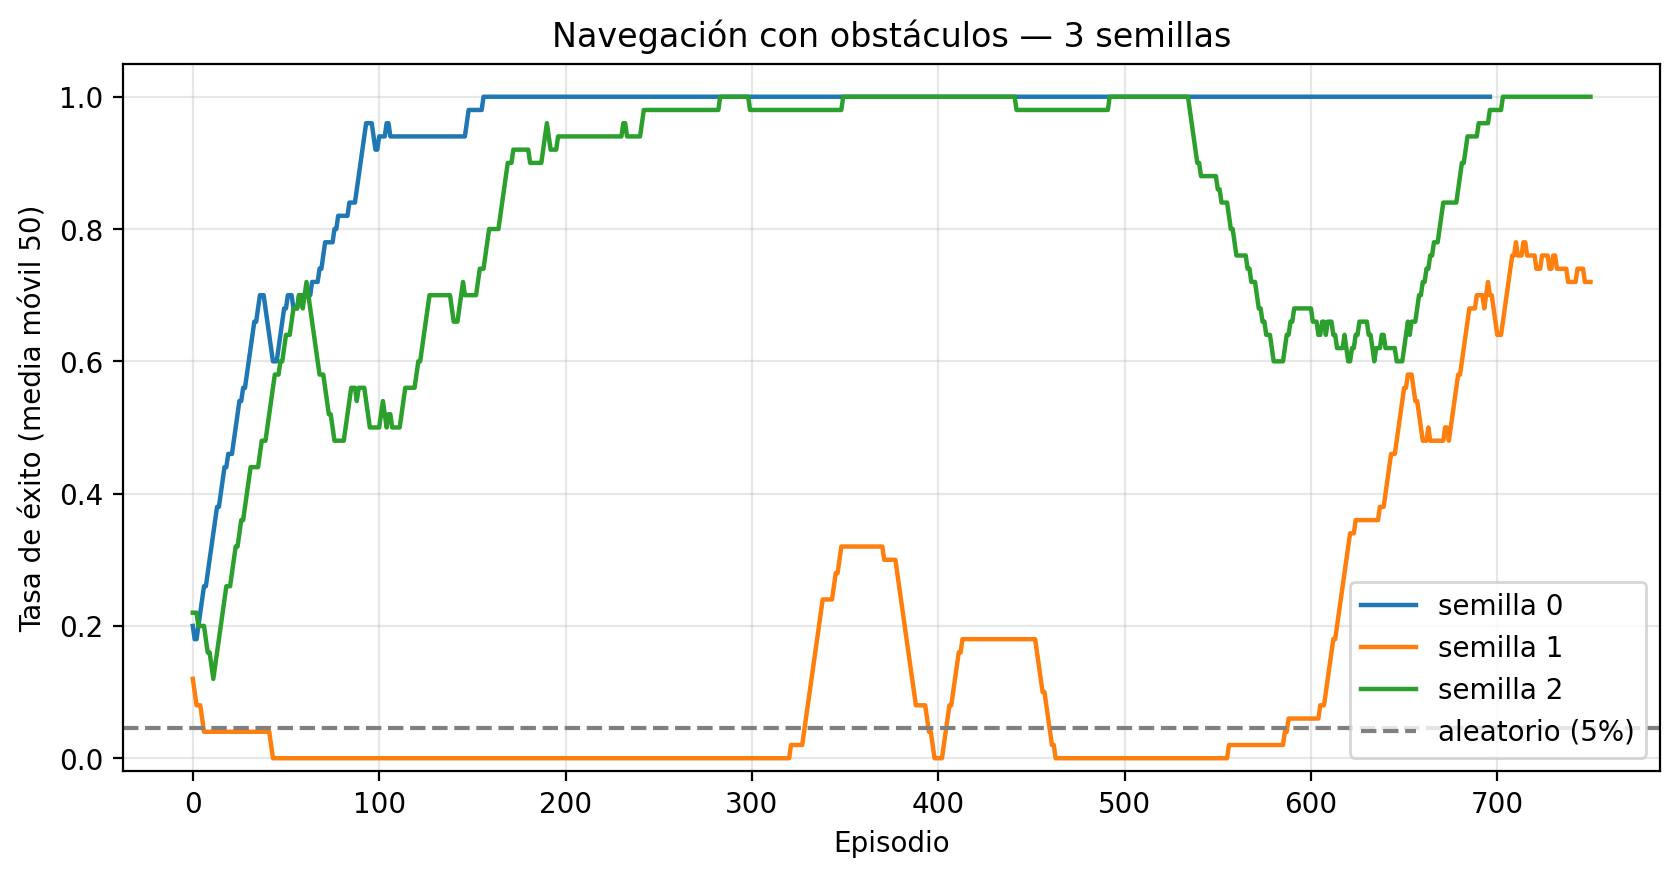
\includegraphics[width=0.72\textwidth]{figuras/obstacle_learning.png}
\caption{Tasa de \'exito de tres corridas del gridworld, suavizada con una ventana de 50 episodios.}
\label{fig:obstacle_learning}
\end{figure}

\subsection{Auto 2D: entorno continuo de conducci\'on}
\label{sec:res_auto2d}

El entorno combina ocho sensores de distancia, direcci\'on y cuatro controles,
con crossbar $24\times8$. El registro disponible indica 5.0\% de \'exito en
los \'ultimos 200 episodios; una evaluaci\'on reportada obtuvo 14\% (7/50) en
test. Solo existe una semilla y faltan los archivos necesarios para
reconstruir la curva y el checkpoint evaluado. Se considera un resultado
piloto, no evidencia de robustez entre semillas.

\subsection{An\'alisis comparativo entre tareas}
\label{sec:comparativa}
\label{sec:interpretacion_comparativa}

La Tabla~\ref{tab:cross_task} resume los \'ultimos 200 episodios de los
registros de presupuesto fijo. Recompensa, exactitud y tasa de llegada
son magnitudes diferentes; adem\'as, las tareas usan matrices y protocolos
distintos. La comparaci\'on es descriptiva y no estima un efecto causal de
la arquitectura ni de la regla de aprendizaje.

\begin{table}[H]
\centering
\small
\caption{Resumen descriptivo de las corridas de presupuesto fijo.}
\label{tab:cross_task}
\begin{tabular}{lccccc}
\toprule
Tarea & Episodios & Semillas & M\'etrica final & $\bar X$ & $\sigma_X$\\
\midrule
CartPole & 300 & 5 & $\bar R_{200}=435.31$ & 0.1379 & 0.0717\\
Visi\'on $8\times8$ & 5000 & 3 & $\mathrm{Acc}_{200}=100\%$ & $\approx0.10$ & 0.022--0.030\\
Navegaci\'on & 746--800 & 3 & $S_{200}=77.17\%$ & 0.221--0.345 & 0.190--0.288\\
Auto 2D & 1000 & 1 & $S_{200}=5.0\%$ & 0.319 & 0.274\\
\bottomrule
\end{tabular}
\end{table}

\subsection{Piloto comparativo REINFORCE/R-STDP}
\label{sec:piloto_rstdp_reinforce}

El lote de parada por \'exito evalu\'o CartPole, visi\'on y obst\'aculos con ambos
algoritmos, semillas 0 y 1 e inicializaciones $X_0=0.1$ y $X_0=0.9$.
Car se ejecut\'o solo con R-STDP. El criterio fue al menos 271 \'exitos dentro
de los \'ultimos 300 episodios (90.33\%), con m\'aximo de 10\,000 episodios;
no exige 300 \'exitos consecutivos. Cada tarea conserva su tama\~no de crossbar
y definici\'on de \'exito. La tabla resume los registros del piloto.

\begin{table}[H]
\centering
\footnotesize
\begin{tabularx}{\textwidth}{l l p{1.5cm} X}
\toprule
Tarea & Regla & Criterio & Episodios / alcance\\
\midrule
CartPole & REINFORCE & 2/4 & 349 y 1249; dos registros incompletos a 559 y 1132.\\
CartPole & R-STDP & 4/4 & 307--1199 episodios.\\
Visi\'on & REINFORCE & 4/4 & 586--1357 episodios.\\
Visi\'on & R-STDP & 4/4 & 470--2951 episodios.\\
Obst\'aculos & REINFORCE & 4/4 & 300 episodios en las cuatro condiciones.\\
Obst\'aculos & R-STDP & 4/4 & 300--336 episodios.\\
Car, lote principal & R-STDP & 1/4 & Una condici\'on a 3775; tres a 10\,000 sin criterio.\\
Car, repetici\'on corregida & R-STDP & 2/4 & Semilla 2: 750 y 1548; semilla 4: ambas a 10\,000 sin criterio.\\
\bottomrule
\end{tabularx}
\caption{Resultado del piloto de parada por \'exito. Cada fracci\'on corresponde a cuatro condiciones semilla--$X_0$, salvo donde se indica el alcance incompleto.}
\label{tab:piloto_rstdp_reinforce}
\end{table}

R-STDP designa el modo implementado en el runner: elegibilidad local
modulada por retorno. La regla STDP local del crossbar s\'i produce cambios;
el piloto muestra que su integraci\'on con la tarea todav\'ia es inestable entre
condiciones y dominios. No se extrapola a hardware. La discusi\'on del evento
post, el baseline y la estabilidad est\'a en el Ap\'endice~\ref{ap:desarrollo_extendido}.

\subsection{Limitaciones}
\label{sec:limitaciones}

Los resultados son de simulaci\'on y no se dispone de un prototipo f\'isico.
Las comparaciones con art\'iculos usan datos digitalizados, a veces con pocos
puntos o protocolos incompletos; las pruebas sint\'eticas no sustituyen
mediciones. Las aplicaciones no comparten una m\'etrica ni un protocolo
id\'enticos. Visi\'on se evalu\'o con variantes de plantillas, navegaci\'on mostr\'o
baja transferencia a mapas nuevos y Auto 2D cuenta con una semilla y
archivos incompletos. El piloto R-STDP alcanza el criterio en algunas
condiciones, pero no permite concluir robustez general. Estas limitaciones
acotan las afirmaciones del trabajo y motivan m\'as semillas, registros
\'integros y protocolos previamente fijados.

\section{An\'alisis de costos}
\label{sec:analisis_costos}

El costo es una estimaci\'on acad\'emica de reproducir simulaciones en una
computadora disponible; no es un registro de gastos ni de horas efectivas.
Se imputan 260 horas a Bs.~20/h y asignaciones de equipo y servicios. No se
incluyen computadora nueva ni hardware memristivo f\'isico.

\begin{table}[H]
\centering
\small
\caption{Estimaci\'on acad\'emica de trabajo e infraestructura.}
\label{tab:costo_total}
\begin{tabular}{lrr}
\toprule
Concepto & Base estimada & Importe\\
\midrule
An\'alisis y dise\~no & 30 h $\times$ Bs.~20/h & Bs.~600\\
Desarrollo e implementaci\'on & 160 h $\times$ Bs.~20/h & Bs.~3\,200\\
Pruebas y validaci\'on & 35 h $\times$ Bs.~20/h & Bs.~700\\
Documentaci\'on y tesis & 35 h $\times$ Bs.~20/h & Bs.~700\\
Trabajo total & 260 h $\times$ Bs.~20/h & Bs.~5\,200\\
Uso de equipo disponible & Estimaci\'on & Bs.~400\\
Electricidad e internet & Estimaci\'on conjunta & Bs.~200\\
\midrule
Total acad\'emico referencial & & Bs.~5\,800\\
\bottomrule
\end{tabular}
\end{table}

Se consolidaron las categor\'ias de costo en una tabla para evitar repetir
los mismos importes en varios res\'umenes. Las tarifas son supuestos de
planificaci\'on, no comprobantes ni consumos medidos.

\else
\chapter{Marco Referencial}

\section{Introducción}

Durante las últimas décadas, el crecimiento exponencial de aplicaciones basadas en inteligencia artificial, aprendizaje automático y procesamiento masivo de datos ha impulsado una demanda cada vez mayor de recursos computacionales. Este fenómeno ha evidenciado las limitaciones presentes en las arquitecturas tradicionales basadas en el modelo de Von Neumann, donde las unidades de procesamiento y almacenamiento se encuentran físicamente separadas. Como consecuencia, una parte significativa del consumo energético total de un sistema computacional se destina al movimiento de información entre memoria y procesador, generando limitaciones de rendimiento conocidas como el cuello de botella de Von Neumann \cite{9,15}.

La necesidad de superar estas restricciones ha motivado el desarrollo de nuevos paradigmas computacionales inspirados en el funcionamiento del sistema nervioso biológico. Entre ellos destaca la computación neuromórfica, cuyo objetivo consiste en integrar almacenamiento y procesamiento dentro de una misma estructura física para reducir el movimiento de datos y mejorar la eficiencia energética \cite{2,15}. Este enfoque busca reproducir características observadas en sistemas biológicos, incluyendo paralelismo masivo, aprendizaje adaptativo y tolerancia a fallos.

Uno de los dispositivos más prometedores para la implementación de sistemas neuromórficos es el memristor. Este elemento fue propuesto teóricamente por Leon Chua en 1971 como el cuarto elemento fundamental de los circuitos eléctricos, complementando al resistor, capacitor e inductor mediante una relación funcional entre flujo magnético y carga eléctrica \cite{17}. Décadas después, Strukov et al. demostraron experimentalmente la existencia física de un dispositivo con comportamiento memristivo basado en óxido de titanio, reactivando el interés científico y tecnológico en esta área de investigación \cite{26}.

Los memristores presentan propiedades particularmente atractivas para aplicaciones neuromórficas. Entre ellas destacan su capacidad de memoria no volátil, la posibilidad de modificar gradualmente su conductancia mediante estímulos eléctricos y la capacidad de conservar estados internos aun cuando la alimentación eléctrica es removida \cite{26,2}. Estas características permiten representar pesos sinápticos artificiales y reproducir mecanismos de aprendizaje inspirados en procesos biológicos.

Diversas investigaciones han demostrado la capacidad de los memristores para implementar fenómenos asociados a la plasticidad sináptica, incluyendo potenciación a largo plazo (Long-Term Potentiation, LTP), depresión a largo plazo (Long-Term Depression, LTD) y plasticidad dependiente del tiempo de disparo (Spike-Timing Dependent Plasticity, STDP) \cite{3,2}. Asimismo, los memristores pueden organizarse en arreglos tipo crossbar que permiten realizar operaciones de computación en memoria y acelerar procesos de inferencia neuronal mediante estructuras altamente paralelas \cite{4,5}.

Sin embargo, el desarrollo de hardware neuromórfico basado en memristores continúa enfrentando desafíos importantes. Los dispositivos reales presentan fenómenos de variabilidad dispositivo a dispositivo (Device-to-Device, D2D) y variabilidad ciclo a ciclo (Cycle-to-Cycle, C2C), generando diferencias estadísticas entre dispositivos nominalmente idénticos \cite{27,29,21}. Adicionalmente, el incremento en la densidad de integración de arreglos crossbar introduce corrientes parásitas conocidas como sneak paths, las cuales afectan la precisión de lectura y escritura de información \cite{7}.

Debido a estas dificultades, la simulación computacional se ha convertido en una herramienta fundamental para el análisis y validación de arquitecturas neuromórficas antes de su implementación física. Herramientas de simulación permiten estudiar el comportamiento de dispositivos memristivos, mecanismos de plasticidad y arquitecturas de interconexión reduciendo costos de desarrollo y facilitando la exploración de nuevas configuraciones experimentales \cite{20,23,24}.

En este contexto, el presente trabajo propone el desarrollo de un simulador neuromórfico basado en memristores capaz de integrar modelado físico del dispositivo, variabilidad estocástica, plasticidad sináptica, neuronas tipo Leaky Integrate-and-Fire y arquitecturas crossbar dentro de una misma plataforma de simulación. La propuesta busca proporcionar una herramienta que permita estudiar fenómenos neuromórficos de forma integrada y validar su comportamiento mediante comparación con resultados reportados en la literatura científica.

\section{Planteamiento del Problema}

La computación neuromórfica se ha consolidado como una de las líneas de investigación más prometedoras para el desarrollo de sistemas capaces de ejecutar tareas de aprendizaje, reconocimiento de patrones y procesamiento cognitivo con una eficiencia energética superior a la ofrecida por las arquitecturas computacionales tradicionales \cite{2,15}. Este interés ha impulsado el desarrollo de dispositivos electrónicos emergentes capaces de emular el comportamiento de neuronas y sinapsis biológicas, siendo los memristores una de las tecnologías más estudiadas debido a sus propiedades de memoria no volátil y modificación gradual de conductancia \cite{17,26}.

A pesar de los avances logrados durante los últimos años, el desarrollo de hardware neuromórfico basado en memristores continúa enfrentando importantes desafíos científicos y tecnológicos. Uno de los principales problemas radica en la complejidad inherente de los dispositivos memristivos reales. A diferencia de los modelos ideales utilizados en etapas iniciales de investigación, los dispositivos físicos presentan fenómenos de variabilidad dispositivo a dispositivo y variabilidad ciclo a ciclo, provocando diferencias significativas en parámetros como voltajes de conmutación, velocidades de transición resistiva y niveles de conductancia alcanzados durante procesos de aprendizaje \cite{27,29,21}.

Estas variaciones afectan directamente el desempeño de sistemas neuromórficos construidos a partir de grandes cantidades de memristores. En aplicaciones prácticas, pequeñas diferencias en el comportamiento individual de los dispositivos pueden generar modificaciones acumulativas en los pesos sinápticos de una red neuronal, alterando procesos de aprendizaje y clasificación \cite{8,2}. Como consecuencia, resulta insuficiente analizar únicamente modelos ideales del memristor, siendo necesario incorporar mecanismos que permitan representar comportamientos estocásticos observados experimentalmente.

Otro desafío importante está relacionado con la integración de los memristores dentro de arquitecturas neuromórficas completas. Diversos trabajos han demostrado la viabilidad de utilizar memristores como sinapsis artificiales y elementos de almacenamiento analógico \cite{3,6}; sin embargo, la evaluación conjunta de dispositivos memristivos, neuronas artificiales y mecanismos de aprendizaje continúa siendo un problema complejo. Con frecuencia, las investigaciones se enfocan únicamente en uno de estos componentes, dificultando el análisis integral del comportamiento del sistema.

De manera similar, los arreglos crossbar memristivos representan una de las arquitecturas más prometedoras para implementar computación en memoria y acelerar operaciones neuronales mediante paralelismo masivo \cite{4,5}. No obstante, el incremento de densidad en estas estructuras introduce fenómenos no deseados, entre ellos las corrientes parásitas conocidas como sneak paths. Estas corrientes generan rutas alternativas para el flujo de información, degradando la precisión de lectura y escritura y limitando la escalabilidad de los sistemas \cite{7}.

La validación experimental de estos fenómenos requiere equipamiento especializado, procesos de fabricación avanzados y recursos económicos considerables. Además, la construcción de prototipos físicos limita la capacidad de explorar rápidamente diferentes configuraciones arquitectónicas y escenarios de operación. Esta situación dificulta el estudio sistemático de la interacción entre comportamiento físico del memristor, plasticidad sináptica, actividad neuronal y arquitecturas de interconexión.

Por otra parte, existen herramientas especializadas orientadas al modelado de memristores, simulación de redes neuronales o análisis de arreglos crossbar \cite{20,23,24}. Sin embargo, muchas de estas soluciones se encuentran enfocadas en problemas específicos y no integran simultáneamente el comportamiento físico del dispositivo, la variabilidad estocástica, los mecanismos de plasticidad sináptica y los efectos arquitectónicos presentes en sistemas neuromórficos de gran escala.

En consecuencia, surge la necesidad de desarrollar una herramienta de simulación que permita analizar de manera integrada los diferentes niveles que conforman un sistema neuromórfico basado en memristores. Una plataforma de estas características facilitaría la evaluación de modelos memristivos, la implementación de neuronas artificiales, el estudio de mecanismos de aprendizaje y el análisis de arquitecturas crossbar bajo condiciones realistas de operación, reduciendo costos experimentales y favoreciendo la investigación en computación inspirada en el cerebro.

\subsection{Definición del Problema}

Actualmente, la investigación en hardware neuromórfico basado en memristores enfrenta dificultades asociadas a la complejidad de modelar simultáneamente el comportamiento físico de los dispositivos, la variabilidad inherente presente en procesos de conmutación resistiva, los mecanismos de plasticidad sináptica y las arquitecturas de interconexión utilizadas en sistemas neuromórficos. La ausencia de herramientas de simulación que integren estos elementos dentro de una misma plataforma limita la capacidad de evaluar y validar diseños neuromórficos antes de su implementación física.

\subsection{Pregunta de Investigación}

¿Con qué nivel de concordancia un simulador neuromórfico basado en memristores puede reproducir el comportamiento de dispositivos memristivos, neuronas LIF, mecanismos de plasticidad sináptica (STDP) y una arquitectura crossbar simplificada, en comparación con los resultados reportados en la literatura científica, considerando además la incorporación de variabilidad estocástica (D2D y C2C)?

\section{Objetivos}

\subsection{Objetivo General}

Desarrollar un simulador neuromórfico basado en memristores que integre el modelado físico del dispositivo, variabilidad estocástica, plasticidad sináptica y una arquitectura crossbar simplificada, con el fin de analizar y validar cuantitativamente su concordancia con resultados reportados en la literatura científica.

\subsection{Objetivos Específicos}

\begin{enumerate}

\item Implementar y validar el modelo memristivo de Strukov, incorporando variabilidad estocástica dispositivo a dispositivo (D2D) y ciclo a ciclo (C2C).

\item Caracterizar el comportamiento dinámico del memristor mediante análisis de histéresis y evolución de estados resistivos bajo diferentes condiciones de excitación.

\item Implementar una neurona tipo Leaky Integrate-and-Fire (LIF) como unidad básica de procesamiento neuronal.

\item Desarrollar una sinapsis memristiva con plasticidad dependiente del tiempo de disparo (STDP) y analizar la evolución del peso sináptico.

\item Integrar los componentes memristor, sinapsis STDP y neurona LIF en una arquitectura crossbar simplificada y analizar su comportamiento colectivo.

\item Validar cuantitativamente los modelos implementados mediante comparación con resultados reportados en la literatura científica, utilizando métricas de error numérico y coincidencia funcional.

\end{enumerate}

\subsection{Criterios de Validación}

La validación de los modelos implementados se realizará mediante dos enfoques complementarios:

\textbf{Validación cuantitativa:} Se compararán las curvas y valores numéricos obtenidos por el simulador con los resultados reportados en la literatura científica, utilizando las siguientes métricas:
\begin{itemize}
\item \textbf{Error relativo porcentual (ERP):} para comparar valores puntuales (voltajes de conmutación, niveles de conductancia, umbrales neuronales).
\item \textbf{Error cuadrático medio (RMSE):} para comparar curvas completas (histéresis I-V, evolución temporal de estados, curvas de aprendizaje STDP).
\item \textbf{Coeficiente de determinación (R$^2$):} para evaluar la calidad del ajuste entre las curvas simuladas y las de referencia.
\end{itemize}

Para una referencia $y_i$ y una predicción alineada $\hat y_i$, el error
cuadrático medio es
$\mathrm{RMSE}=\sqrt{\frac{1}{n}\sum_{i=1}^{n}(y_i-\hat y_i)^2}$ y conserva
las unidades de la magnitud comparada. En este trabajo, el error relativo
porcentual (ERP) de una curva se calcula como
$100\,\max_i|y_i-\hat y_i|/(\max_i y_i-\min_i y_i)$; se normaliza por el
rango de la referencia y no es el error porcentual punto a punto. Cuando
se comparan parámetros escalares, el ERP se calcula respecto al valor de
referencia correspondiente.

\textbf{Validación cualitativa:} Se evaluará la coincidencia funcional de los fenómenos reproducidos, verificando que el simulador capture correctamente:
\begin{itemize}
\item La forma de la curva de histéresis del memristor (figura en forma de lazo).
\item La dependencia exponencial de la plasticidad sináptica respecto al intervalo de tiempo entre pulsos (ventana STDP).
\item El comportamiento de integración y disparo de la neurona LIF (umbral, período refractario, frecuencia de disparo vs. corriente inyectada).
\item La respuesta colectiva de la arquitectura crossbar ante patrones de entrada conocidos.
\end{itemize}

Se considerará que un modelo está \textbf{validado} cuando cumpla simultáneamente: ERP $<$ 10\% en parámetros clave, R$^2$ $>$ 0.90 en comparación de curvas, y coincidencia cualitativa completa con el fenómeno reportado.

\section{Límites y Alcances}

\subsection{Límites}

Toda investigación requiere establecer límites que definan claramente el alcance de los resultados obtenidos y permitan delimitar el problema de estudio. En este trabajo, los límites establecidos responden a la naturaleza computacional del proyecto y a la necesidad de concentrar los esfuerzos en el análisis de sistemas neuromórficos basados en memristores.

La presente investigación se limita al desarrollo de un simulador computacional orientado al análisis de dispositivos memristivos y arquitecturas neuromórficas. Por tanto, no contempla la fabricación física de memristores ni la implementación experimental de circuitos electrónicos sobre hardware real.

El comportamiento de los dispositivos memristivos será representado mediante modelos matemáticos obtenidos de la literatura científica, incorporando fenómenos de variabilidad y comportamiento estocástico reportados experimentalmente. En consecuencia, los resultados obtenidos corresponderán a simulaciones numéricas y no a mediciones directas realizadas sobre dispositivos físicos.

La investigación se enfocará principalmente en el estudio de neuronas tipo Leaky Integrate-and-Fire (LIF), por lo que otros modelos neuronales más complejos, tales como Hodgkin-Huxley, FitzHugh-Nagumo o Izhikevich, no serán considerados dentro del alcance del presente trabajo.

Los mecanismos de aprendizaje implementados estarán limitados a procesos de plasticidad sináptica basados en STDP, utilizando memristores como elementos de almacenamiento de peso sináptico. No se abordarán otros esquemas de aprendizaje supervisado o no supervisado de mayor complejidad computacional.

Asimismo, el análisis arquitectónico estará centrado en arreglos crossbar memristivos simplificados. No se abordará la implementación de arquitecturas neuromórficas especializadas de gran escala ni sistemas comerciales de computación neuromórfica.

Finalmente, la validación de los modelos implementados se realizará mediante comparación con resultados reportados en la literatura científica, sin considerar procesos de caracterización experimental sobre dispositivos fabricados específicamente para esta investigación.

\subsection{Alcances}

El simulador desarrollado permitirá representar el comportamiento dinámico de dispositivos memristivos basados en el modelo de Strukov, incorporando fenómenos de variabilidad dispositivo a dispositivo y ciclo a ciclo observados en dispositivos reales.

La plataforma permitirá analizar características fundamentales del memristor, incluyendo curvas de histéresis corriente-voltaje, evolución temporal de estados resistivos, modificación gradual de conductancia y efectos asociados a procesos de conmutación resistiva.

Dentro del ámbito neuromórfico, el simulador incorporará neuronas tipo Leaky Integrate-and-Fire para representar mecanismos básicos de integración temporal y generación de pulsos neuronales. Estas neuronas podrán interactuar con sinapsis memristivas para reproducir comportamientos inspirados en procesos biológicos de aprendizaje.

Asimismo, se implementará un mecanismo de plasticidad sináptica basado en STDP, permitiendo estudiar la evolución de pesos sinápticos bajo diferentes patrones de estimulación neuronal.

La investigación también incluirá la implementación de arreglos crossbar memristivos simplificados orientados al análisis de arquitecturas de computación en memoria. Estas estructuras permitirán evaluar el comportamiento colectivo de múltiples dispositivos memristivos y estudiar fenómenos asociados al procesamiento paralelo de información.

Finalmente, los modelos implementados serán validados mediante comparación con resultados reportados en la literatura científica, incluyendo trabajos relacionados con modelado memristivo, plasticidad sináptica, redes neuromórficas y arreglos crossbar, proporcionando evidencia cuantitativa y cualitativa de la capacidad del simulador para reproducir fenómenos observados en investigaciones previas.

\section{Justificación}

La computación neuromórfica se ha consolidado como una de las principales alternativas para superar las limitaciones energéticas y de escalabilidad presentes en las arquitecturas computacionales tradicionales. Dentro de este contexto, los memristores han despertado un creciente interés debido a su capacidad para almacenar información de forma no volátil y modificar gradualmente su conductancia, características que permiten representar el comportamiento de sinapsis biológicas \cite{2,26}.

A pesar de los avances reportados en la literatura, el desarrollo experimental de sistemas neuromórficos basados en memristores continúa enfrentando desafíos asociados a la fabricación de dispositivos, la variabilidad inherente de los procesos de conmutación resistiva y la complejidad de validar arquitecturas de gran escala \cite{21,27,29}. Como consecuencia, las herramientas de simulación desempeñan un papel fundamental al permitir el análisis de estos fenómenos antes de la implementación física de los sistemas.

Desde una perspectiva científica, el presente trabajo contribuye al estudio de la relación existente entre el comportamiento físico de los memristores y los mecanismos de aprendizaje inspirados biológicamente. La integración de modelos memristivos, plasticidad sináptica, neuronas artificiales y arquitecturas crossbar dentro de una misma plataforma permite analizar fenómenos neuromórficos de manera integral y facilita la reproducción de resultados reportados en investigaciones previas \cite{3,7}.

Desde el punto de vista tecnológico, el simulador propuesto proporciona una herramienta capaz de evaluar configuraciones neuromórficas sin necesidad de recurrir inicialmente a procesos de fabricación especializados, reduciendo costos de desarrollo y facilitando la exploración de nuevas arquitecturas de computación en memoria \cite{5,11}.

Finalmente, desde una perspectiva académica, la investigación integra conocimientos de electrónica, modelado matemático, sistemas dinámicos e inteligencia artificial, contribuyendo a la formación en un área de creciente relevancia para el desarrollo de tecnologías inspiradas en el cerebro.
\chapter{Marco Teórico}

El presente capítulo expone los principales antecedentes científicos y tecnológicos relacionados con el desarrollo de sistemas neuromórficos basados en memristores. Se analizan diferentes enfoques reportados en la literatura científica, incluyendo el modelado físico de dispositivos memristivos, la incorporación de fenómenos de variabilidad estocástica, la implementación de redes neuromórficas basadas en memristores y el estudio de arquitecturas crossbar. Posteriormente, se presentan los fundamentos teóricos necesarios para comprender el funcionamiento de los modelos y algoritmos implementados en esta investigación.

\section{Estado del Arte}

Durante las últimas décadas, el desarrollo de dispositivos memristivos ha impulsado nuevas líneas de investigación orientadas a la construcción de sistemas computacionales inspirados en el cerebro biológico. La posibilidad de integrar almacenamiento y procesamiento dentro de una misma estructura física ha convertido a los memristores en una de las tecnologías más prometedoras para la computación neuromórfica. Como consecuencia, numerosos trabajos han abordado distintos aspectos relacionados con modelado físico, variabilidad, aprendizaje sináptico y arquitecturas de computación en memoria.

A continuación, se presentan los principales enfoques identificados en la literatura científica que sustentan el desarrollo de la presente investigación.

\subsection{Enfoque 1}

Uno de los hitos más importantes en el área de dispositivos electrónicos emergentes fue la formulación teórica del memristor realizada por Leon Chua en 1971. En dicho trabajo se propuso la existencia de un cuarto elemento fundamental de circuito capaz de establecer una relación directa entre la carga eléctrica y el flujo magnético, complementando al resistor, capacitor e inductor tradicionales \cite{17}. Aunque inicialmente se trató de una propuesta teórica, este concepto abrió una nueva línea de investigación orientada al desarrollo de dispositivos con capacidad de memoria integrada.

Décadas después, Strukov et al. demostraron experimentalmente la existencia física de un dispositivo con comportamiento memristivo basado en una estructura de dióxido de titanio (\ce{TiO2}) \cite{26}. Este trabajo constituye uno de los pilares fundamentales de la investigación moderna en memristores, ya que proporciona un modelo matemático capaz de describir la evolución temporal del estado interno del dispositivo mediante una variable de estado asociada al desplazamiento de vacancias de oxígeno.

El modelo propuesto por Strukov describe un dispositivo compuesto por dos regiones con diferentes niveles de conductividad. La frontera entre ambas regiones varía en función de la corriente aplicada, modificando el valor instantáneo de resistencia del dispositivo. Como resultado, el memristor presenta una característica de histéresis en el plano corriente-voltaje, permitiendo almacenar información sin necesidad de alimentación continua \cite{26}.

La simplicidad matemática del modelo de Strukov ha favorecido su utilización en simulaciones y estudios académicos. Sin embargo, investigaciones posteriores han demostrado que los dispositivos reales presentan comportamientos más complejos que aquellos descritos por el modelo ideal. Trabajos recientes han incorporado efectos físicos adicionales, restricciones de frontera y mecanismos no lineales para mejorar la representación de dispositivos memristivos fabricados experimentalmente \cite{21,28}.

A pesar de sus limitaciones, el modelo de Strukov continúa siendo una referencia fundamental debido a su capacidad para capturar los principios esenciales del comportamiento memristivo y proporcionar una base sólida para el desarrollo de modelos más avanzados. Por esta razón, numerosos simuladores y plataformas de investigación utilizan este modelo como punto de partida para la implementación de sistemas neuromórficos basados en memristores.

\subsection{Enfoque 2}

Aunque los modelos ideales permiten comprender los principios fundamentales de operación de un memristor, diversos estudios experimentales han demostrado que los dispositivos físicos presentan fenómenos de variabilidad que afectan significativamente su comportamiento eléctrico. Estas variaciones pueden manifestarse tanto entre dispositivos fabricados bajo condiciones nominalmente idénticas como entre diferentes ciclos de operación de un mismo dispositivo \cite{27,29}.

La variabilidad dispositivo a dispositivo, conocida como Device-to-Device (D2D), se encuentra asociada a diferencias estructurales introducidas durante los procesos de fabricación. Por otra parte, la variabilidad ciclo a ciclo, denominada Cycle-to-Cycle (C2C), se relaciona con fluctuaciones presentes durante procesos repetitivos de escritura y borrado. Ambos fenómenos generan dispersión en parámetros como voltajes de conmutación, resistencia de encendido y resistencia de apagado \cite{29}.

Con el objetivo de representar estas características, diversos autores han propuesto modelos estocásticos capaces de incorporar incertidumbre dentro del comportamiento memristivo. Estos modelos incluyen distribuciones probabilísticas para parámetros físicos y mecanismos de transición resistiva, permitiendo reproducir comportamientos observados experimentalmente que no pueden ser capturados mediante modelos deterministas convencionales \cite{27,8}.

La incorporación de variabilidad constituye un aspecto particularmente importante para aplicaciones neuromórficas, ya que las diferencias entre dispositivos pueden afectar procesos de aprendizaje, almacenamiento de información y estabilidad de redes neuronales. Como consecuencia, los modelos modernos de memristores tienden a integrar mecanismos estocásticos que permitan aproximar con mayor precisión el comportamiento observado en dispositivos reales \cite{21,29}.

\subsection{Enfoque 3}

La utilización de memristores dentro de sistemas neuromórficos ha dado lugar a una importante línea de investigación orientada a la implementación de sinapsis artificiales capaces de reproducir mecanismos de aprendizaje inspirados en procesos biológicos. Dentro de este contexto, uno de los trabajos más influyentes corresponde a la investigación desarrollada por Prezioso et al., quienes demostraron la operación de una red neuromórfica integrada basada en memristores de óxido metálico \cite{3}.

El trabajo de Prezioso evidenció la posibilidad de emplear memristores como elementos de almacenamiento de pesos sinápticos dentro de redes neuronales artificiales. Mediante la modificación gradual de la conductancia de los dispositivos, los autores lograron implementar procesos de aprendizaje capaces de clasificar patrones de entrada sin necesidad de entrenamiento externo complejo \cite{3}.

Paralelamente, diversos estudios han demostrado que los memristores pueden reproducir fenómenos de plasticidad sináptica observados en sistemas biológicos. Entre ellos destacan la potenciación a largo plazo (LTP), la depresión a largo plazo (LTD) y la plasticidad dependiente del tiempo de disparo (STDP), mecanismos considerados fundamentales para procesos de aprendizaje y adaptación neuronal \cite{2}.

Estos avances han consolidado a los memristores como una de las tecnologías más prometedoras para el desarrollo de hardware neuromórfico, permitiendo implementar sinapsis artificiales compactas, energéticamente eficientes y capaces de almacenar información de forma no volátil \cite{6}.

\subsection{Enfoque 4}

El crecimiento de las redes neuromórficas basadas en memristores ha impulsado el desarrollo de arquitecturas capaces de conectar grandes cantidades de dispositivos dentro de una misma estructura física. Entre las alternativas más estudiadas destacan los arreglos tipo crossbar, los cuales permiten organizar memristores en forma matricial para realizar operaciones de computación en memoria mediante mecanismos altamente paralelos \cite{4,5}.

Las arquitecturas crossbar presentan ventajas importantes en términos de densidad de integración, eficiencia energética y velocidad de procesamiento. Debido a que cada memristor puede representar un peso sináptico individual, estas estructuras resultan especialmente adecuadas para implementar redes neuronales artificiales y sistemas de inferencia neuromórfica \cite{5}.

Sin embargo, el incremento del tamaño de los arreglos crossbar introduce fenómenos no ideales que afectan su funcionamiento, tales como corrientes parásitas y degradación del margen de ruido, los cuales han sido ampliamente estudiados en la literatura como limitaciones de escalabilidad \cite{7}. En el contexto de la presente investigación, se abordará el análisis de arreglos crossbar simplificados, dejando el estudio de estos fenómenos de escala masiva como una extensión natural para trabajos futuros.

\subsection{Discusión}

Los enfoques analizados evidencian la evolución progresiva de la investigación en sistemas neuromórficos basados en memristores. El modelo de Strukov proporciona una base matemática sólida para describir el comportamiento fundamental del dispositivo, mientras que los estudios de variabilidad permiten aproximar con mayor precisión las características observadas en dispositivos reales. Por otra parte, las investigaciones orientadas a redes neuromórficas demuestran la capacidad de los memristores para implementar mecanismos de aprendizaje inspirados biológicamente, y los estudios sobre arquitecturas crossbar muestran su potencial para desarrollar sistemas de computación en memoria de alta densidad.

Sin embargo, la mayoría de los trabajos revisados abordan estos aspectos de forma independiente. En consecuencia, existe la necesidad de contar con herramientas capaces de integrar modelado memristivo, variabilidad estocástica, plasticidad sináptica y análisis arquitectónico dentro de una misma plataforma. Esta necesidad constituye la principal motivación para el desarrollo del simulador neuromórfico propuesto en la presente investigación.

\section{Fundamentos Teóricos}

La presente investigación integra conceptos provenientes de la electrónica, la computación neuromórfica y el modelado matemático de dispositivos memristivos. En esta sección se presentan los fundamentos teóricos necesarios para comprender el funcionamiento de los modelos implementados dentro del simulador propuesto. Se abordan los principios de operación del memristor, los mecanismos de variabilidad presentes en dispositivos reales, los modelos neuronales utilizados en sistemas neuromórficos y las arquitecturas de interconexión empleadas para la implementación de redes neuronales basadas en memristores.

\subsection{Memristor}

El memristor fue propuesto por Leon Chua en 1971 como el cuarto elemento fundamental de los circuitos eléctricos, complementando al resistor, capacitor e inductor \cite{17}. Su principal característica consiste en establecer una relación funcional entre la carga eléctrica acumulada y el flujo magnético asociado al dispositivo.

A diferencia de un resistor convencional, cuya resistencia permanece constante para un determinado valor de temperatura, el memristor posee una resistencia dependiente de la historia de excitaciones eléctricas previamente aplicadas. Como consecuencia, el dispositivo es capaz de almacenar información incluso después de retirar la alimentación eléctrica, propiedad conocida como memoria no volátil.

Matemáticamente, la relación fundamental propuesta por Chua puede expresarse como:

\begin{equation}
d\phi=M(q)dq
\end{equation}

donde $\phi$ representa el flujo magnético, $q$ corresponde a la carga eléctrica acumulada y $M(q)$ define la memristancia del dispositivo.

Esta característica permite que el memristor conserve información acerca de estados previos, convirtiéndolo en un candidato ideal para representar sinapsis artificiales dentro de sistemas neuromórficos \cite{17,26}.

\subsection{Modelo de Strukov}
\label{sec:convenciones_estado}

La primera demostración experimental de un dispositivo memristivo fue realizada por Strukov et al. en 2008 mediante una estructura basada en dióxido de titanio (\ce{TiO2}) \cite{26}. El dispositivo se encuentra formado por dos regiones con diferente conductividad: una región dopada con alta conductancia y una región no dopada con baja conductancia.

La resistencia total del dispositivo puede expresarse mediante:

\begin{equation}
R(w)=R_{ON}\frac{w}{D}+R_{OFF}\left(1-\frac{w}{D}\right)
\end{equation}

Definiendo la fracción dopada normalizada $x=w/D\in[0,1]$, la expresión
equivalente es $R(x)=R_{ON}x+R_{OFF}(1-x)$. En esta tesis se usa también
la variable complementaria $X=1-x$, que representa la fracción no dopada:
\[
R(X)=R_{ON}+X(R_{OFF}-R_{ON}).
\]
Ambas expresiones son equivalentes. En el simulador del agente se emplea
$X$ porque la matriz de estado del crossbar se representa directamente con
esta variable y la conductancia se obtiene como $G=1/R(X)$. Todas las medias
y desviaciones de $X$ reportadas en el Capítulo~3 corresponden a esta
variable de estado; no son estadísticas de $G$.

La Tabla~\ref{tab:convenciones_memristor} resume los símbolos y su
interpretación.

\begin{table}[H]
\centering
\small
\caption{Convenciones de variables y parámetros del memristor y del crossbar.}
\label{tab:convenciones_memristor}
\begin{tabularx}{\textwidth}{c X c c X}
\hline
\textbf{Símbolo} & \textbf{Definición} & \textbf{Unidades} &
\textbf{Rango} & \textbf{Efecto} \\
\hline
$w$ & Ancho de la región dopada & m & [0,$D$] & Aumenta al crecer la región dopada \\
$D$ & Espesor total de la capa activa & m & $D>0$ & Normaliza la posición de la frontera \\
$x$ & Fracción dopada, $x=w/D$ & -- & [0,1] & Si $x$ aumenta, $R$ disminuye \\
$X$ & Fracción no dopada, $X=1-x$ & -- & [0,1] & Si $X$ aumenta, $R$ aumenta \\
$R$ & Resistencia del dispositivo & $\Omega$ & [$R_{ON},R_{OFF}$] & -- \\
$G$ & Conductancia, $G=1/R$ & S & [$1/R_{OFF},1/R_{ON}$] & -- \\
$w_s$ & Peso sináptico normalizado & -- & [0,1] & Si $w_s$ aumenta, $G$ aumenta \\
\hline
\end{tabularx}
\end{table}

En la notación de la tabla:

\begin{itemize}
\item $R_{ON}$ representa la resistencia mínima.
\item $R_{OFF}$ representa la resistencia máxima.
\item $D$ corresponde al espesor total del dispositivo.
\item $w$ define la posición de la frontera entre las regiones dopada y no dopada.
\end{itemize}

La evolución temporal ideal de la variable de estado se encuentra
dada por:

\begin{equation}
\frac{dx}{dt}=\frac{1}{D}\frac{dw}{dt}
=\mu_v\frac{R_{ON}}{D^2}i(t)
\end{equation}

donde $\mu_v$ representa la movilidad efectiva de vacancias de
oxígeno e $i(t)$ corresponde a la corriente que atraviesa el
dispositivo. En la configuración Strukov--Biolek del simulador, esta
dinámica se multiplica además por la función de ventana
$f_B(x,i)=1-(x-\operatorname{stp}(-i))^{2p}$, con $p=5$, para atenuar
la evolución al acercarse a los límites del estado, donde
$\operatorname{stp}(-i)=1$ si $i<0$ y $0$ en caso contrario. El
estado inicial del archivo de configuración es $x_0=0.1$. Si el agente
deriva su estado complementario de ese valor sin una sobrescritura,
resulta $X_0=1-x_0=0.9$. Sin embargo, la configuración de CartPole
analizada pasa explícitamente \texttt{initial\_X=0.1}; por tanto, en
esas corridas el valor explícito prevalece y equivale a $x_0=0.9$.
Esta distinción entre el parámetro del dispositivo y el estado inicial
explícito del agente se mantiene en la tabla de parámetros del
Capítulo~3.

Este modelo permite reproducir la característica de histéresis observada experimentalmente en memristores y constituye la base de numerosos simuladores utilizados en investigación neuromórfica \cite{26}.

\subsection{Variabilidad Estocástica en Memristores}

Aunque el modelo de Strukov permite describir adecuadamente los principios fundamentales de operación de un memristor, diversos estudios experimentales han demostrado que los dispositivos físicos presentan comportamientos que difieren de las predicciones obtenidas mediante modelos ideales \cite{21,27,29}. Estas diferencias se encuentran asociadas a procesos de fabricación, defectos estructurales, fluctuaciones térmicas y mecanismos microscópicos involucrados en la formación y ruptura de filamentos conductivos.

Uno de los fenómenos más importantes observados en dispositivos memristivos reales corresponde a la variabilidad estocástica. Este comportamiento se manifiesta mediante diferencias en los parámetros eléctricos de dispositivos nominalmente idénticos y mediante fluctuaciones observadas durante ciclos repetidos de operación.

La variabilidad suele clasificarse en dos categorías principales:

\begin{itemize}
\item Variabilidad dispositivo a dispositivo (Device-to-Device, D2D).
\item Variabilidad ciclo a ciclo (Cycle-to-Cycle, C2C).
\end{itemize}

La variabilidad D2D se encuentra asociada a diferencias introducidas durante los procesos de fabricación. Factores como el espesor de las capas activas, la distribución de defectos cristalinos y la concentración de vacancias pueden generar diferencias significativas entre dispositivos fabricados bajo condiciones aparentemente idénticas \cite{29}.

Por otra parte, la variabilidad C2C se produce cuando un mismo dispositivo presenta respuestas diferentes durante ciclos consecutivos de escritura y borrado. Este fenómeno está relacionado con la naturaleza probabilística de los procesos de migración iónica y formación de filamentos conductivos \cite{27}.

Como consecuencia, parámetros como la resistencia de encendido ($R_{ON}$), la resistencia de apagado ($R_{OFF}$), los voltajes de conmutación y la conductancia alcanzada después de cada pulso pueden presentar distribuciones estadísticas en lugar de valores únicos deterministas.

La incorporación de mecanismos estocásticos dentro de los modelos memristivos resulta particularmente importante en aplicaciones neuromórficas. A diferencia de sistemas digitales convencionales, donde la variabilidad suele considerarse una fuente de error, diversos estudios han demostrado que ciertos niveles de aleatoriedad pueden contribuir positivamente a procesos de aprendizaje y adaptación inspirados biológicamente \cite{8}.

Por esta razón, los simuladores modernos de sistemas neuromórficos incorporan modelos probabilísticos capaces de representar fenómenos de variabilidad observados experimentalmente, permitiendo aproximar con mayor precisión el comportamiento de dispositivos físicos reales \cite{21,27,29}.

\subsection{Neurona Leaky Integrate-and-Fire}

Las neuronas constituyen la unidad básica de procesamiento dentro del sistema nervioso biológico. Su función principal consiste en integrar señales provenientes de múltiples sinapsis y generar impulsos eléctricos cuando la actividad acumulada supera un determinado umbral.

Dentro de los diferentes modelos neuronales existentes, la neurona Leaky Integrate-and-Fire (LIF) representa una de las aproximaciones más utilizadas debido a su simplicidad matemática y capacidad para reproducir los mecanismos fundamentales de integración temporal observados en neuronas biológicas.
Su formulación constituye una aproximación clásica en el modelado de neuronas de disparo \cite{36}.

El modelo LIF considera que el potencial de membrana evoluciona de acuerdo con la ecuación:

\begin{equation}
\tau_m \frac{dV_m}{dt}=-(V_m-V_{rest})+RI(t)
\end{equation}

donde:

\begin{itemize}
\item $V_m$ representa el potencial de membrana.
\item $V_{rest}$ corresponde al potencial de reposo.
\item $\tau_m$ es la constante de tiempo de la membrana.
\item $R$ representa la resistencia equivalente.
\item $I(t)$ corresponde a la corriente de entrada.
\end{itemize}

La neurona integra continuamente la corriente recibida desde sus entradas. Cuando el potencial de membrana alcanza un valor umbral previamente definido, la neurona genera un pulso de salida o \textit{spike}.

Posteriormente, el potencial de membrana es reiniciado a un valor de reposo, iniciando nuevamente el proceso de integración.

La simplicidad computacional del modelo LIF ha favorecido su utilización en sistemas neuromórficos y simuladores de redes neuronales de gran escala. Asimismo, su comportamiento resulta adecuado para estudiar mecanismos de plasticidad sináptica basados en el tiempo relativo de ocurrencia de eventos neuronales.

\subsection{Plasticidad Sináptica}

La capacidad de aprendizaje del sistema nervioso biológico se encuentra estrechamente relacionada con la plasticidad sináptica, proceso mediante el cual la intensidad de conexión entre neuronas puede modificarse en respuesta a diferentes patrones de actividad neuronal. Este mecanismo permite que las redes neuronales adapten su comportamiento a partir de experiencias previas, constituyendo una de las bases fundamentales del aprendizaje y la memoria.

En sistemas neuromórficos, los memristores resultan particularmente adecuados para representar sinapsis artificiales debido a su capacidad para modificar y conservar estados de conductancia de manera no volátil. Como consecuencia, numerosos trabajos han explorado el uso de dispositivos memristivos para implementar mecanismos de plasticidad inspirados en procesos biológicos \cite{2,3}.

En la literatura se documentan diversos fenómenos de plasticidad, entre los cuales destacan la Potenciación a Largo Plazo (LTP) y la Depresión a Largo Plazo (LTD), que describen cambios progresivos en la eficacia sináptica tras estímulos repetitivos. Estos fenómenos constituyen la base conceptual de múltiples mecanismos de aprendizaje en sistemas neuromórficos.

No obstante, uno de los mecanismos de aprendizaje más importantes y biológicamente relevantes en neurociencia computacional corresponde a la Plasticidad Dependiente del Tiempo de Disparo (Spike-Timing Dependent Plasticity, STDP). Este mecanismo establece que la modificación de una conexión sináptica depende de la diferencia temporal precisa entre los disparos de una neurona presináptica y una neurona postsináptica.

Si la neurona presináptica dispara antes que la neurona postsináptica, la conexión sináptica tiende a fortalecerse. Por el contrario, si la neurona postsináptica dispara antes que la neurona presináptica, la conexión tiende a debilitarse.

Una ventana STDP exponencial ideal puede expresarse como referencia
conceptual, siguiendo los estudios de plasticidad dependiente del
tiempo y dispositivos memristivos \cite{33,30}:

\begin{equation}
\Delta w =
\begin{cases}
A_{+}e^{-\Delta t/\tau_{+}}, & \Delta t > 0 \\
-A_{-}e^{\Delta t/\tau_{-}}, & \Delta t < 0
\end{cases}
\end{equation}

donde:

\begin{itemize}
\item $\Delta w$ representa la variación del peso sináptico.
\item $\Delta t$ corresponde a la diferencia temporal entre disparos.
\item $A_{+}$ y $A_{-}$ definen las amplitudes de potenciación y depresión.
\item $\tau_{+}$ y $\tau_{-}$ representan constantes temporales del proceso.
\end{itemize}

Con $w_0=0$, la regla STDP implementada en
\texttt{neurolab.synapses.stdp} normaliza el cambio porcentual de
conductancia:
\begin{equation}
\Delta G_{ij}
=G_{ij}\frac{p_{\max}}{100}f(\Delta t), \qquad
f(\Delta t)=
\begin{cases}
e^{-\Delta t/\tau_{+}}, & \Delta t>0,\\
-e^{\Delta t/\tau_{-}}, & \Delta t<0,\\
0, & \Delta t=0,
\end{cases}
\end{equation}
El valor $p_{\max}=0.5\%$ por evento corresponde al parámetro
\texttt{max\_percent\_change} de \texttt{STDPRule}.
Esta normalización preserva la forma exponencial y limita el cambio
respecto de la conductancia actual; la forma ideal en $\Delta w$
anterior se conserva como referencia conceptual.

Los valores digitalizados atribuidos a Jo et al. en
\texttt{jo2010\_stdp.csv} presentan asimetría: los cambios observados
incluyen $-18.48\%$ a $\Delta t=-8.64$ ms y $+12.63\%$ a
$\Delta t=9.01$ ms. Un ajuste exponencial de mínimos cuadrados por
separado a los puntos de cada signo da los parámetros de referencia
de la Tabla~\ref{tab:parametros_stdp}. Este ajuste a puntos
digitalizados no se interpreta como una medición adicional ni como
una parametrización que el agente utilice.

\begin{table}[H]
\centering
\caption{Parámetros de la ventana STDP: ajuste a la serie atribuida a Jo et al. y configuración del módulo local.}
\label{tab:parametros_stdp}
\begin{tabular}{lcc}
\hline
\textbf{Parámetro} & \textbf{Ajuste a serie Jo et al.} & \textbf{Módulo \texttt{STDPRule}} \\
\hline
$A_{+}$ & $16.12\%$ & $0.05$ \\
$|A_{-}|$ (magnitud) & $25.58\%$ & $A_{-}=-0.025$ \\
$\tau_{+}$ & $40.50~\mathrm{ms}$ & $17~\mathrm{ms}$ \\
$\tau_{-}$ & $23.55~\mathrm{ms}$ & $34~\mathrm{ms}$ \\
$p_{\max}$ & -- & $0.5\%$ por evento \\
\hline
\end{tabular}
\end{table}

El ajuste se realizó sobre la magnitud de cada rama, con
$|\Delta w|=|A_{\pm}|\exp(-|\Delta t|/\tau_{\pm})$; por ello
$|A_{-}|>|A_{+}|$ en la serie digitalizada. Los parámetros del
módulo son valores normalizados de configuración (adimensionales),
donde $A_{-}$ se guarda con signo negativo, y no se sustituyen por
el ajuste de referencia.
En \texttt{STDPRule}, $A_{+}$ y $A_{-}$ normalizan la fracción
aplicada a la conductancia; con $w_0=0$ se cancelan en esa operación.
Por tanto, el coeficiente porcentual máximo es $p_{\max}$ para ambas
ramas y la asimetría de la respuesta de conductancia procede de las
constantes temporales, no de los valores configurados de $A_{\pm}$.
El ajuste no lineal de mínimos cuadrados presentó RMSE de
$1.35$ puntos porcentuales para la rama de potenciación y
$1.04$ puntos porcentuales para la rama de depresión. Debido a su
capacidad para modificar gradualmente la conductancia en función de estímulos eléctricos,
los memristores constituyen una plataforma adecuada para implementar
mecanismos STDP \cite{2,3}. El módulo STDP se conserva para el
análisis de plasticidad del sustrato; la regla REINFORCE con baseline
del agente se describe por separado en el Capítulo~3.

\subsection{Arquitecturas Crossbar Memristivas}

Uno de los principales desafíos en la implementación de sistemas neuromórficos consiste en conectar un gran número de neuronas y sinapsis de forma eficiente. Para abordar este problema, los memristores suelen organizarse en estructuras matriciales conocidas como arreglos crossbar, las cuales permiten implementar redes neuronales de alta densidad mediante una disposición regular de filas y columnas conductoras \cite{4,5}.

Un arreglo crossbar está formado por un conjunto de líneas horizontales y verticales que se intersectan entre sí. En cada punto de intersección se ubica un dispositivo memristivo cuya conductancia representa el peso sináptico asociado a una conexión neuronal. Esta organización permite almacenar grandes cantidades de información dentro de un área física reducida y facilita la implementación de operaciones de computación en memoria.

La principal ventaja de las arquitecturas crossbar radica en su capacidad para realizar operaciones de multiplicación matriz-vector directamente sobre el hardware. Esta característica resulta especialmente relevante para redes neuronales artificiales, ya que gran parte de los procesos de inferencia y aprendizaje pueden expresarse mediante este tipo de operaciones matemáticas.

Considerando un vector de entrada representado por tensiones aplicadas a las filas del arreglo, la corriente obtenida en cada columna puede expresarse mediante la Ley de Ohm y la Ley de Corrientes de Kirchhoff como:

\begin{equation}
I_j=\sum_{i=1}^{N} G_{ij}V_i
\end{equation}

Con la convención de este trabajo, $\mathbf{G}\in\mathbb{R}^{N\times M}$
tiene una fila por entrada y una columna por salida, mientras que
$\mathbf{V}\in\mathbb{R}^{N}$ contiene los voltajes aplicados a las
filas. Por tanto, el vector de corrientes de columna es
$\mathbf{I}=\mathbf{G}^{\mathsf T}\mathbf{V}\in\mathbb{R}^{M}$.

donde:

\begin{itemize}
\item $I_j$ representa la corriente de salida en la columna $j$.
\item $V_i$ corresponde a la tensión aplicada en la fila $i$.
\item $G_{ij}$ representa la conductancia del memristor ubicado en la intersección $(i,j)$.
\end{itemize}

Esta ecuación muestra que el arreglo crossbar realiza de manera natural una multiplicación matriz-vector, donde la matriz de conductancias actúa como conjunto de pesos sinápticos de la red neuronal.

Gracias a esta propiedad, los arreglos crossbar han sido ampliamente estudiados como una alternativa para implementar computación en memoria, reduciendo significativamente el movimiento de datos entre memoria y procesador característico de las arquitecturas tradicionales \cite{5}. Asimismo, su elevada densidad de integración los convierte en una de las estructuras más prometedoras para el desarrollo de hardware neuromórfico escalable.

En el contexto de esta investigación, se analizan arreglos crossbar
simplificados para evaluar el comportamiento colectivo de múltiples
dispositivos memristivos y su integración con neuronas LIF. El
protocolo de lectura del agente resuelve mediante MNA la red eléctrica
incluida en su topología y considera resistencias de línea y de
sensado, como se detalla en la siguiente sección. Esto no equivale a
simular todas las configuraciones de \textit{sneak paths}, en
particular la prueba clásica con líneas no seleccionadas flotantes.
El análisis de escalabilidad a arreglos de alta densidad, selectores y
margen de ruido se considera una extensión para trabajos futuros
\cite{7}.

\subsection{Sneak Paths y Margen de Ruido}

A medida que aumenta el tamaño de los arreglos crossbar memristivos, aparecen fenómenos eléctricos que no están presentes en estructuras de pequeña escala. Uno de los más importantes corresponde a las corrientes parásitas conocidas como \textit{Sneak Paths}, las cuales constituyen uno de los principales obstáculos para la implementación de sistemas memristivos de alta densidad \cite{7}.

Un Sneak Path aparece cuando la corriente eléctrica encuentra rutas alternativas distintas de la trayectoria prevista durante operaciones de lectura o escritura. Debido a la naturaleza altamente interconectada de los arreglos crossbar, la corriente puede propagarse a través de múltiples dispositivos memristivos, generando contribuciones no deseadas que alteran el valor medido en la celda objetivo.

La presencia de estas corrientes produce errores en la estimación de estados resistivos y puede afectar significativamente la precisión de operaciones realizadas sobre el arreglo. Este problema se vuelve especialmente crítico cuando el número de filas y columnas aumenta, ya que la cantidad de rutas alternativas disponibles crece rápidamente con el tamaño de la matriz \cite{7}.

Otro parámetro importante asociado al desempeño de arreglos crossbar corresponde al margen de ruido (\textit{Noise Margin}). Este parámetro permite cuantificar la capacidad del sistema para distinguir correctamente entre diferentes estados lógicos o resistivos en presencia de perturbaciones eléctricas.

Una reducción excesiva del margen de ruido incrementa la probabilidad de errores durante operaciones de lectura y limita la escalabilidad de la arquitectura. Como consecuencia, numerosos estudios han propuesto técnicas orientadas a minimizar los efectos de Sneak Paths mediante modificaciones arquitectónicas, dispositivos selectores o estrategias de polarización especializadas \cite{7}.

El análisis de \textit{sneak paths} y margen de ruido resulta
fundamental para evaluar la viabilidad de arquitecturas neuromórficas
basadas en memristores. En este trabajo, la lectura del crossbar del
agente se resuelve mediante análisis nodal modificado (MNA), con
resistencias de línea $R_{\mathrm{wire}}=1\,\mathrm{m}\Omega$ y de
sensado $R_{\mathrm{sense}}=100\,\Omega$. El solver representa las
corrientes y caídas de tensión que resultan de esa red modelada; el
Experimento~10 evalúa el acoplamiento entre columnas bajo la excitación
indicada. No se implementó la configuración clásica de lectura con una
celda seleccionada y las demás líneas flotantes, ni la dinámica de
programación/escritura con rutas parásitas. Esos casos y la
caracterización física de hardware quedan fuera del alcance.

\subsection{Parámetros del modelo de referencia}
\label{subsec:parametros-modelo}

La Tabla~\ref{tab:parametros_modelo} reúne los valores de la
configuración Strukov--Biolek y del agente CartPole usada como
referencia. Los valores de lectura y aprendizaje corresponden al
protocolo del agente; los parámetros eléctricos y LIF se convierten a
unidades SI desde los archivos JSON.

\begin{table}[H]
\centering
\small
\caption{Parámetros del dispositivo, crossbar y agente de referencia.}
\label{tab:parametros_modelo}
\begin{tabularx}{\textwidth}{c c c X X}
\hline
\textbf{Símbolo} & \textbf{Valor} & \textbf{Unidad} &
\textbf{Fuente} & \textbf{Uso} \\
\hline
$R_{\mathrm{ON}}$ & $100$ & $\Omega$ &
\texttt{strukov\_ideal.json} & Strukov y agente \\
$R_{\mathrm{OFF}}$ & $16\,000$ & $\Omega$ &
\texttt{strukov\_ideal.json} & Strukov y agente \\
$D$ & $10$ & $\mathrm{nm}$ &
\texttt{strukov\_ideal.json} & Modelo Strukov \\
$\mu_v$ & $10^{-14}$ & $\mathrm{m^2/(V\,s)}$ &
\texttt{strukov\_ideal.json} & Modelo Strukov \\
$x_0$ & $0.1$ & adimensional &
\texttt{strukov\_ideal.json} & Estado físico inicial; $X_0=0.1$ en el agente \\
$X_0$ & $0.1$ & adimensional &
\texttt{run\_robot.py} & Estado inicial del agente; equivale a $x_0=0.9$ \\
$p$ (Biolek) & $5$ & adimensional &
\texttt{strukov\_ideal.json} & Ventana de frontera \\
$V_{\mathrm{th}}$ (Strukov) & $0.1$ & $\mathrm{V}$ &
\texttt{StrukovConfig}, \texttt{StrukovMathModel} &
Umbral predeterminado del modelo; no medido fisicamente \\
$V_{\mathrm{read}}$ & $0.05$ & $\mathrm{V}$ &
\texttt{run\_robot.py} & Rail de lectura; ruta MNA sin actualizacion de X \\
$R_{\mathrm{wire}}$ & $10^{-3}$ & $\Omega$ &
\texttt{crossbar\_brain.py} & Solver MNA del agente \\
$R_{\mathrm{sense}}$ & $100$ & $\Omega$ &
\texttt{crossbar\_brain.py} & Solver MNA del agente \\
$C_m$ & $100$ & $\mathrm{nF}$ &
\texttt{lif\_config.json} & Neurona LIF \\
$R_{\mathrm{series}}$ & $100$ & $\mathrm{k}\Omega$ &
\texttt{lif\_config.json} & Neurona LIF \\
$R_{\mathrm{leak}}$ & $1$ & $\mathrm{M}\Omega$ &
\texttt{lif\_config.json} & Neurona LIF \\
$V_{\mathrm{th,LIF}}$ & $1.0$ & $\mathrm{V}$ &
\texttt{lif\_config.json} & Umbral LIF \\
$t_{\mathrm{ref}}$ & $2\times10^{-3}$ & $\mathrm{s}$ &
\texttt{lif\_config.json}, \texttt{lab\_bridge.py} &
LIF (el JSON almacena $2$ ms y el puente lo convierte a segundos) \\
$\eta$ & $0.005$ & adimensional &
\texttt{run\_robot.py} & Tasa de aprendizaje REINFORCE \\
$T_{\mathrm{init}}$ & $1.0$ o $0.05$ & adimensional &
\texttt{run\_robot.py} & Temperatura inicial seleccionable \\
$T_{\min}$ & $0.05$ & adimensional &
\texttt{run\_robot.py} & Temperatura mínima \\
$T_{\mathrm{decay}}$ & $0.995$ & adimensional &
\texttt{run\_robot.py} & Decaimiento de temperatura por episodio \\
$W_b$ & $200$ & episodios &
\texttt{run\_robot.py} & Ventana del baseline móvil \\
\hline
\end{tabularx}
\end{table}
\chapter{Marco Práctico}

El presente capítulo describe la implementación y validación del
simulador neuromórfico desarrollado. Primero se presentan la
arquitectura general del sistema y las herramientas empleadas;
después, la metodología seguida, desde el modelado del dispositivo
memristivo hasta su integración en un agente de control autónomo.
Finalmente, se exponen los resultados de las simulaciones y se
estima el costo de reproducirlas.

Las Etapas 1--4 del desarrollo del sustrato (modelo memristivo y
variabilidad, neurona LIF, plasticidad sináptica y crossbar) se
documentan en ese orden en el Apéndice~\ref{ap:desarrollo_extendido}.
Este capítulo resume su integración en el agente y presenta las
aplicaciones evaluadas, sin asignarles números de etapa adicionales.

% =====================================================
\section{Esquema general del proyecto}
% =====================================================

La solución desarrollada se estructuró como un ecosistema 
computacional compuesto por dos subsistemas acoplados. El 
primero, denominado \textit{Neuromorphic Lab}, constituye el
motor de simulación encargado de modelar dispositivos memristivos,
neuronas tipo Leaky Integrate-and-Fire y arreglos crossbar con 
efectos no ideales. El segundo, denominado \textit{Robot Sim}, 
implementa un agente de control autónomo que utiliza el arreglo 
crossbar simulado como sustrato de pesos de su política.

La Figura~\ref{fig:esquema_general} presenta la organización 
general de ambos subsistemas y su relación unidireccional: el 
simulador robótico consume los modelos físicos del laboratorio 
a través de una capa de abstracción (\textit{lab\_bridge}), 
pero el laboratorio no conoce la existencia del agente.

\begin{figure}[H]
\centering
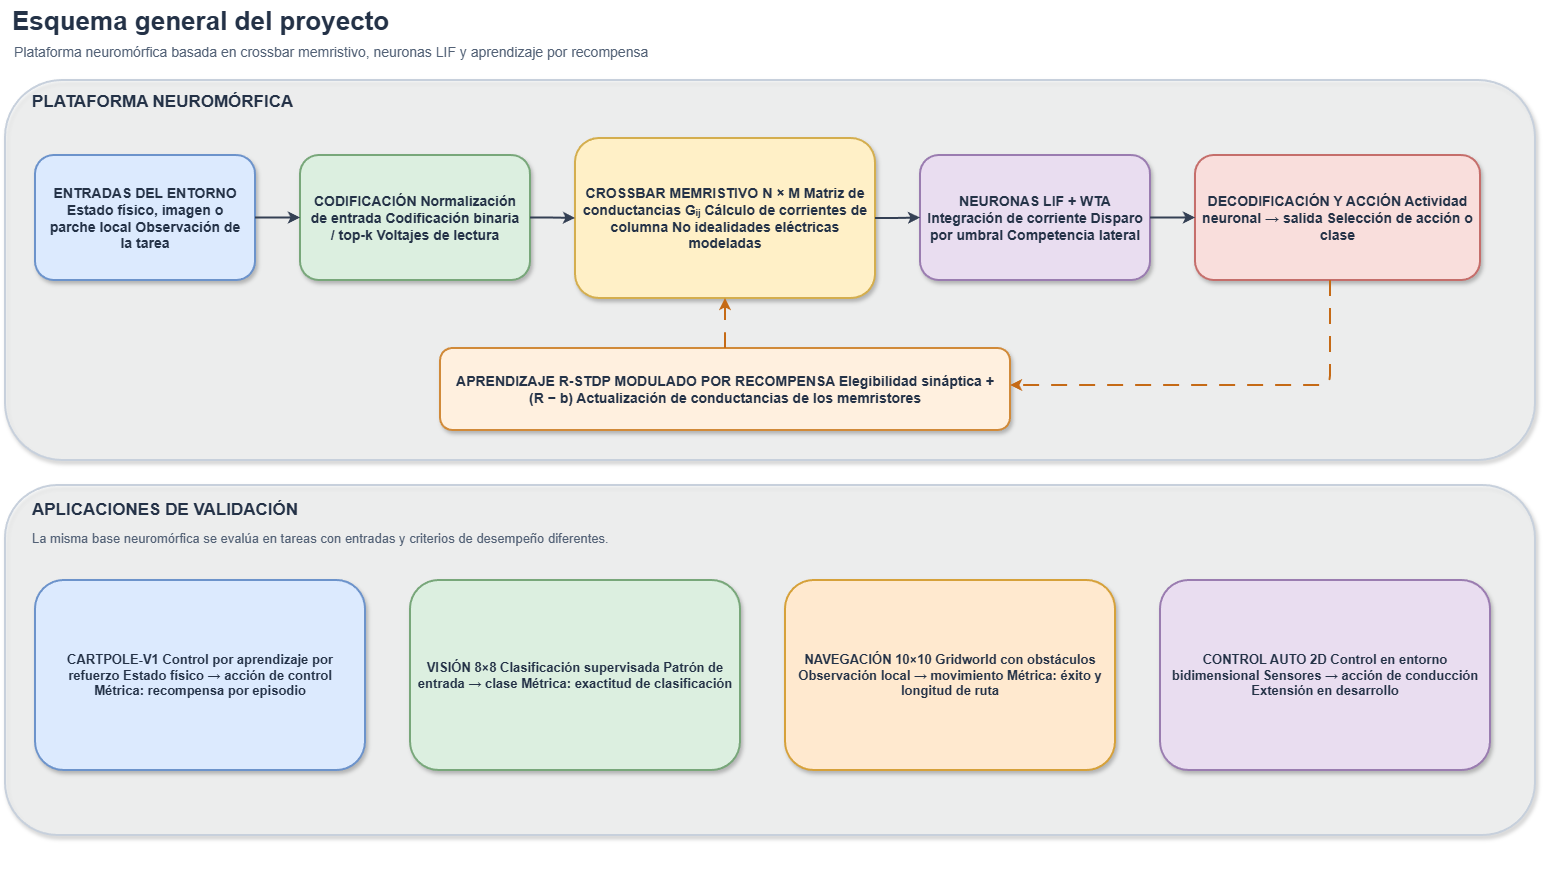
\includegraphics[width=0.86\textwidth]{figuras/esquema_general.png}
\caption[Arquitectura general del ecosistema]{Arquitectura general del ecosistema. El laboratorio 
(\textit{arriba}) provee los modelos físicos; el simulador 
robótico (\textit{abajo}) los integra en un agente de control.}
\label{fig:esquema_general}
\end{figure}

El flujo de información del agente sigue la secuencia 
\textit{sensores} $\rightarrow$ \textit{codificador} 
$\rightarrow$ \textit{crossbar} $\rightarrow$ \textit{decodificador} 
$\rightarrow$ \textit{actuadores}, con el aprendizaje aplicado al 
final de cada episodio mediante una regla de plasticidad 
modulada por recompensa. El detalle de cada componente se 
desarrolla en la Sección~\ref{sec:desarrollo}.

% =====================================================
\section{Herramientas}

El proyecto se desarrolló con herramientas de código abierto,
sin dependencias de software propietario. La Tabla~\ref{tab:hardware} y la
Tabla~\ref{tab:software} listan los componentes principales utilizados.

\subsection{Hardware}

\begin{table}[H]
\centering
\caption{Herramientas de hardware utilizadas.}
\label{tab:hardware}
\begin{tabular}{lp{9cm}}
\hline
\textbf{Componente} & \textbf{Uso} \\
\hline
Laptop de desarrollo & Ejecución de simulaciones y scripts Python (CPU x86-64, 8 GB RAM, SSD) \\
\hline
\end{tabular}
\end{table}

\subsection{Software}

\begin{table}[H]
\centering
\caption{Herramientas de software utilizadas.}
\label{tab:software}
\begin{tabular}{lp{9cm}}
\hline
\textbf{Herramienta} & \textbf{Uso} \\
\hline
Python 3.10+ & Lenguaje principal del simulador \\
NumPy & Álgebra lineal y matrices del crossbar \\
Matplotlib & Generación de figuras y visualización \\
PySide6 & Interfaces gráficas del laboratorio neuromórfico \\
Tkinter & Diálogos de configuración de las aplicaciones \\
Git & Control de versiones \\
\hline
\end{tabular}
\end{table}

% =====================================================

% =====================================================
\section{Metodolog\'ia del agente neurom\'orfico}
\label{sec:metodologia_agente}
\label{sec:desarrollo}

El agente recibe el estado del entorno, lo codifica en entradas del crossbar,
lee sus corrientes de columna y convierte la salida neuronal en una acci\'on.
El arreglo constituye el sustrato de pesos; el entorno y la recompensa se
simulan en software. El desarrollo detallado de los dispositivos, la LIF,
la plasticidad y el solver se documenta en el Ap\'endice~\ref{ap:desarrollo_extendido}.

\subsection{Configuraci\'on de referencia}

CartPole usa un crossbar de $24\times12$, lectura a $0.05\,\mathrm{V}$ y
una neurona LIF por salida. El estado normalizado $X$ se convierte en
resistencia mediante $R(X)=R_{\mathrm{on}}+X(R_{\mathrm{off}}-R_{\mathrm{on}})$;
por ello, $X$ es un estado interno del modelo y no una conductancia. La
configuraci\'on nominal es $R_{\mathrm{on}}=100\,\Omega$,
$R_{\mathrm{off}}=16\,\mathrm{k}\Omega$, $X_0=0.1$ y l\'imites
$0\leq X\leq1$. La tabla resume los par\'ametros el\'ectricos y temporales
usados como referencia.

\begin{table}[H]
\centering
\small
\caption{Par\'ametros de referencia del agente CartPole.}
\label{tab:parametros_agente}
\begin{tabular}{lll}
\toprule
Par\'ametro & Configuraci\'on & Valor efectivo\\
\midrule
$R_{\mathrm{on}}$ & $100\,\Omega$ & $100\,\Omega$\\
$R_{\mathrm{off}}$ & $16\,\mathrm{k}\Omega$ & $16\,000\,\Omega$\\
Estado inicial & $X_0=0.1$ & $x_0=0.9$ bajo $X=1-x$\\
$V_{\mathrm{read}}$ & $0.05\,\mathrm{V}$ & $0.05\,\mathrm{V}$\\
$V_{\mathrm{th}}$ LIF & $1.0\,\mathrm{V}$ & $1.0\,\mathrm{V}$\\
$t_{\mathrm{ref}}$ & $2\,\mathrm{ms}$ & $2\times10^{-3}\,\mathrm{s}$\\
$dt$ & -- & $10^{-4}\,\mathrm{s}$\\
\bottomrule
\end{tabular}
\end{table}

En CartPole, las observaciones se codifican en filas activas; el solver
nodal MNA calcula las corrientes considerando la conductancia del crossbar
y las resistencias configuradas de l\'inea y sensado. Las neuronas LIF
integran las corrientes, generan spikes al alcanzar el umbral y se reinician
seg\'un el per\'iodo refractario. La decisi\'on de acci\'on se obtiene de la
actividad de salida. Estos pasos describen el simulador, no un circuito
fabricado.

La lectura del agente calcula $G(X)$ y resuelve la red MNA sin integrar la
dinamica no volatil del estado durante ese paso; el metodo de lectura no
llama a la actualizacion de las celdas, por lo que en esta ruta simulada
$\Delta X=0$ por construccion. Esto cuantifica el cambio de estado impuesto
por el software en cada lectura, no una perturbacion electrica medida en un
dispositivo fisico. El modelo Strukov del laboratorio si incorpora un
umbral de deriva ionica de $0.1\,\mathrm{V}$ como valor predeterminado
de \texttt{StrukovConfig}; ese umbral se aplica al integrar la dinamica de la celda y no es una medicion
experimental del umbral del dispositivo. El dispositivo volatil de salida,
en cambio, si se actualiza en cada paso y modula la corriente que recibe
la LIF.

\subsection{Reglas de aprendizaje y decisi\'on}

En REINFORCE, el agente conserva una elegibilidad por conexi\'on durante el
episodio y la actualiza al terminarlo seg\'un el retorno y un baseline. La
contribuci\'on instant\'anea es
\[
e_{ij,t}=\mathrm{pre}_{i,t}
\left(\mathbf{1}_{j=\mathrm{col}_t}-\pi_{j,t}\right),\qquad
E_{ij,t}=\gamma E_{ij,t-1}+e_{ij,t},
\]
donde $\pi_{j,t}$ es la probabilidad softmax de la columna $j$. La softmax
convierte puntuaciones en probabilidades que suman uno: una temperatura alta
reparte m\'as la probabilidad y una baja la concentra. El decoder muestrea
seg\'un esa distribuci\'on y la regla de aprendizaje ajusta el crossbar con el
resultado del episodio. Esta forma de gradiente de pol\'itica se basa en REINFORCE y en los m\'etodos
de aprendizaje por refuerzo descritos en la literatura~\cite{Williams1992REINFORCE,SuttonBarto2018}. La implementaci\'on se describe en
\url{robot_sim/neurobot/reinforce_agent.py} y
\url{robot_sim/neurobot/crossbar_brain.py}.

La regla local STDP del laboratorio usa spikes binarios pre/post y trazas
exponenciales $p_i$ y $q_j$:
\[
\tau_{\mathrm{pre}}\dot p_i=-p_i+s_i^{\mathrm{pre}},\qquad
\tau_{\mathrm{post}}\dot q_j=-q_j+s_j^{\mathrm{post}},\qquad
\Delta G_{ij}^{\mathrm{STDP}}=\eta\left(A_+p_i s_j^{\mathrm{post}}
-A_-s_i^{\mathrm{pre}}q_j\right).
\]
En la regla R-STDP del m\'odulo, la elegibilidad decae y acumula ese cambio:
\[
E_{ij,t}=e^{-dt/\tau_e}E_{ij,t-1}+\Delta G_{ij,t}^{\mathrm{STDP}},
\qquad \Delta G_{ij,t}^{\mathrm{R-STDP}}=R_tE_{ij,t}.
\]
Esta formulaci\'on de elegibilidad modulada por recompensa sigue el marco
conceptual de R-STDP~\cite{Izhikevich2007RSTD}; en este proyecto, la regla
local implementada se describe en \url{neurolab/crossbar/plasticity.py}.

Las corridas del agente etiquetadas R-STDP en el Ap\'endice
\ref{ap:evidencia_entrenamientos} no implementan esa regla estricta con
spikes LIF como evento post. En los entornos de control, el runner construye
un evento de acci\'on centrado por la pol\'itica,
$z_{j,t}=\mathbf{1}_{j=a_t}-\pi_{j,t}$, y una elegibilidad por decisi\'on
$e_{ij,t}=a_+\,\mathrm{pre}_{i,t}\max(z_{j,t},0)
+a_-\,\mathrm{pre}_{i,t}\min(z_{j,t},0)$. Los spikes LIF y los ganadores
WTA se registran, pero no sustituyen a $z_{j,t}$ en esta actualizaci\'on;
la tarea de visi\'on usa una elegibilidad derivada del gradiente de corriente.
Para cada paso se calcula el retorno descontado $G_t=r_t+\gamma G_{t+1}$,
la ventaja $A_t=G_t-b_t$ respecto al baseline temporal previo y su
normalizaci\'on $\widehat A_t=A_t/s_A$, donde
$s_A=\max(\operatorname{std}(A),10^{-8})$ (se usa $s_A=1$ para un solo
paso). La elegibilidad modulada del episodio es
\[
E^R_{ij}=\frac{1}{\sqrt{T}}\sum_{t=0}^{T-1} e_{ij,t}\widehat A_t,
\qquad \Delta X=-\eta E^R.
\]
El cambio se escala para cumplir el l\'imite configurado de
$\max_{ij}|\Delta X_{ij}|$ y se anula en episodios que alcanzan el umbral
de congelamiento. La actualizaci\'on opera directamente sobre el estado
abstracto $X$ y las variabilidades D2D/C2C modifican el incremento aplicado.
Para $E^R>0$, $\Delta X<0$ reduce $R(X)$ y aumenta $G(X)$; el signo opuesto
produce el efecto contrario. Esta comprobaci\'on algebraica confirma la
direcci\'on del mapeo en el c\'odigo, pero no demuestra aprendizaje estable
ni programaci\'on por pulsos f\'isicos. Por ello, en
esta tesis las corridas del runner se describen como el piloto h\'ibrido
pre/acci\'on modulado por retorno (conservando R-STDP como nombre del modo
del software), no como evidencia de R-STDP can\'onica pre/post. La variante
de tarea que s\'i emple\'o spikes LIF reales como evento post tuvo bajo
rendimiento exploratorio. Los resultados y su alcance se informan en la
Secci\'on~\ref{sec:piloto_rstdp_reinforce}; la topolog\'ia y el modelo
el\'ectrico del crossbar se mantienen entre reglas de aprendizaje.

\subsection{Aplicaciones evaluadas}

La misma organizaci\'on se adapt\'o a cuatro tareas. Se conservaron la lectura
del crossbar y la actualizaci\'on por recompensa; las dimensiones y el
significado de la salida dependen del entorno. Los registros por condici\'on
se incluyen en el Ap\'endice~\ref{ap:evidencia_entrenamientos}.

\begin{table}[H]
\centering
\small
\caption{Configuraci\'on de las aplicaciones simuladas.}
\label{tab:aplicaciones}
\begin{tabularx}{\textwidth}{l c X X}
\toprule
Tarea & Crossbar & Entrada y salida & M\'etrica\\
\midrule
CartPole & $24\times12$ & Estado continuo; dos acciones & Recompensa y supervivencia\\
Visi\'on & $64\times8$ & Patr\'on binario $8\times8$; ocho clases & Exactitud\\
Obst\'aculos & $16\times4$ & Sensores del gridworld; cuatro movimientos & Llegada a meta\\
Auto 2D & $24\times8$ & Rayos, direcci\'on y distancia; cuatro controles & Llegada a meta\\
\bottomrule
\end{tabularx}
\end{table}

\section{Validaci\'on de modelos}
\label{sec:validacion_modelos}

La validaci\'on se organiz\'o en tres niveles: comprobaciones internas de
c\'odigo y unidades, comparaci\'on de series simuladas con puntos digitalizados
de publicaciones y pruebas funcionales de las aplicaciones. Solo se
presentan m\'etricas cuando existe correspondencia punto a punto y protocolo
definido. Una coincidencia visual, una distribuci\'on sint\'etica o una traza
producida por el mismo modelo no equivalen a una medici\'on de hardware. El
inventario de fuentes y scripts est\'a en el ap\'endice de datos; los protocolos
completos se conservan en el Ap\'endice~\ref{ap:desarrollo_extendido}.

\begin{figure}[H]
\centering
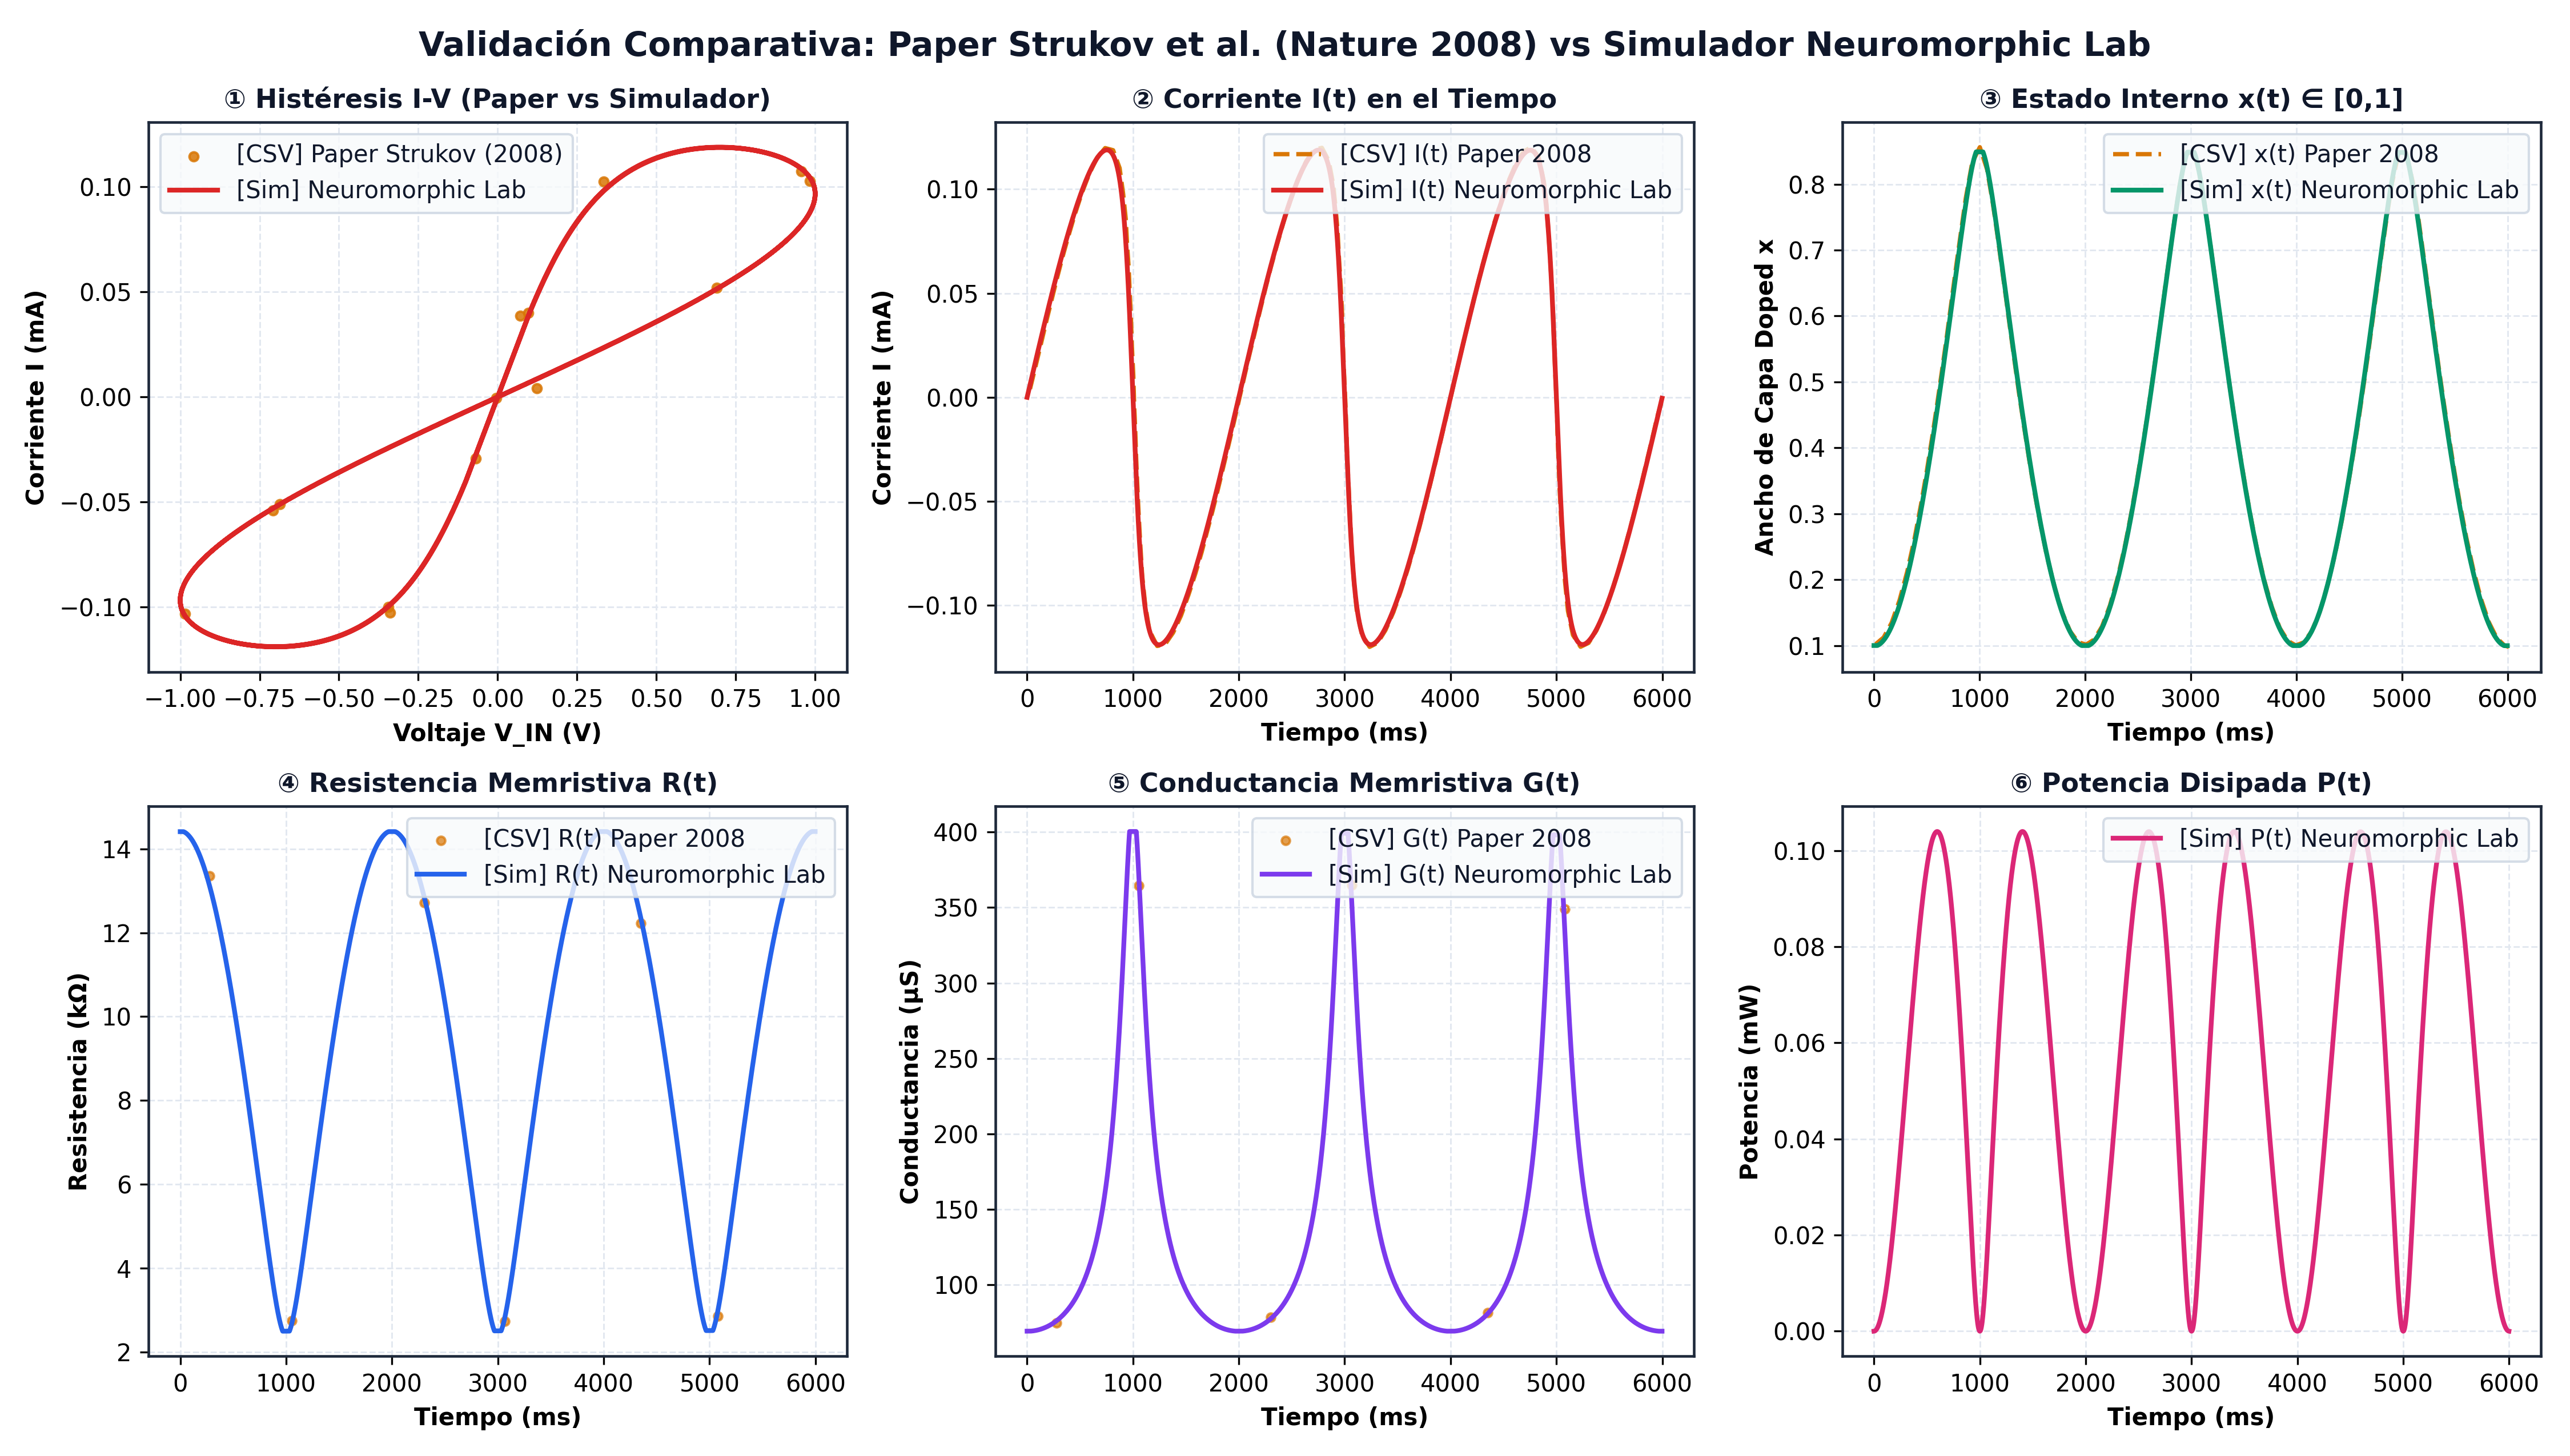
\includegraphics[width=0.78\textwidth]{figuras/fig_01_strukov.png}
\caption{Curvas del modelo Strukov local comparadas con las series digitalizadas atribuidas a la referencia.}
\label{fig:strukov_iv}
\end{figure}

\subsection{Comparaciones cuantitativas}

Para Strukov se compararon estado, corriente, resistencia y conductancia
con series digitalizadas atribuidas al art\'iculo de 2008. Prezioso es una
comparaci\'on visual, pues los puntos no contienen protocolo temporal
completo. La ventana STDP usa nueve puntos de ajuste y cuatro reservados;
LTP/LTD usa 18 puntos de test. La LIF $f-I$ compara Euler con la soluci\'on
anal\'itica del mismo modelo, no con mediciones experimentales. La tabla
resume las m\'etricas reproducibles.

\begin{table}[H]
\centering
\footnotesize
\caption{M\'etricas de validaci\'on reproducibles. $R^2$ es el coeficiente de determinaci\'on; ERP se normaliza por el rango de referencia.}
\label{tab:metricas_validacion}
\begin{tabularx}{\textwidth}{X c c c c c}
\toprule
Comparaci\'on & $n$ & $R^2$ & MAE & RMSE & ERP (\%)\\
\midrule
Strukov, estado $x(t)$ &107&0.999657&0.003676&0.004491&1.27\\
Strukov, corriente $I(t)$ &136&0.996994&0.002586 mA&0.004126 mA&6.22\\
Strukov, resistencia $R(t)$ &87&0.998319&0.135431 k$\Omega$&0.162264 k$\Omega$&3.54\\
Strukov, conductancia $G(t)$ &87&0.983726&7.55759 $\mu$S&15.64415 $\mu$S&19.04\\
Prezioso, $I(V)$ visual &179&--&--&--&--\\
STDP, holdout &4&0.94220&1.90404 pp&2.13626 pp&14.87\\
LTP/LTD, test &18&0.73988&8.3491 nA&8.6181 nA&31.23\\
LIF $f-I$, Euler vs anal\'itica &14&0.999964&0.086431 Hz&0.151393 Hz&0.55\\
\bottomrule
\end{tabularx}
\end{table}

STDP y LTP/LTD proceden de conjuntos digitalizados peque\~nos; sus par\'ametros
ajustados son efectivos y no caracterizan independientemente un dispositivo.
En LTP/LTD, el resultado agregado oculta un ajuste deficiente por rama.
Prezioso carece de etiquetas temporales y de rama suficientes para una
m\'etrica. La prueba D2D/C2C verifica propiedades estad\'isticas de muestras
sint\'eticas, no una poblaci\'on experimental. Las Figuras
\ref{fig:stdp_curve_ch3} y \ref{fig:ltp_ltd_curve_ch3} permiten inspeccionar
los datos atribuidos a Jo et al.; las particiones y limitaciones se ampl\'ian
en el ap\'endice t\'ecnico.

\begin{table}[H]
\centering
\footnotesize
\caption{Cumplimiento de los umbrales cuantitativos cuando son aplicables.}
\label{tab:estado_criterios_modelos}
\begin{tabularx}{\textwidth}{l c c X}
\toprule
Prueba & ERP $<10\%$ & $R^2>0.90$ & Conclusi\'on\\
\midrule
Strukov: $x$, $I$, $R$ & S\'i & S\'i & Cumplen en las series comparadas.\\
Strukov: $G$ & No & S\'i & ERP $=19.04\%$; no cumple todos los umbrales.\\
STDP, holdout ($n=4$) & No & S\'i & Parcial; ERP $=14.87\%$ y muestra peque\~na.\\
LTP/LTD ($n=18$) & No & No & No cumple; $R^2=0.73988$, ERP $=31.23\%$.\\
Prezioso $I(V)$ & No calculable & No calculable & Comparaci\'on visual; faltan puntos con protocolo suficiente.\\
LIF $f-I$ & S\'i$^*$ & S\'i$^*$ & Verificaci\'on interna frente a soluci\'on anal\'itica, no validaci\'on experimental independiente.\\
\bottomrule
\end{tabularx}
\par\smallskip\scriptsize $^*$M\'etricas de integraci\'on para el mismo modelo anal\'itico; no se interpretan como concordancia con hardware publicado.
\end{table}

\begin{figure}[H]
\centering
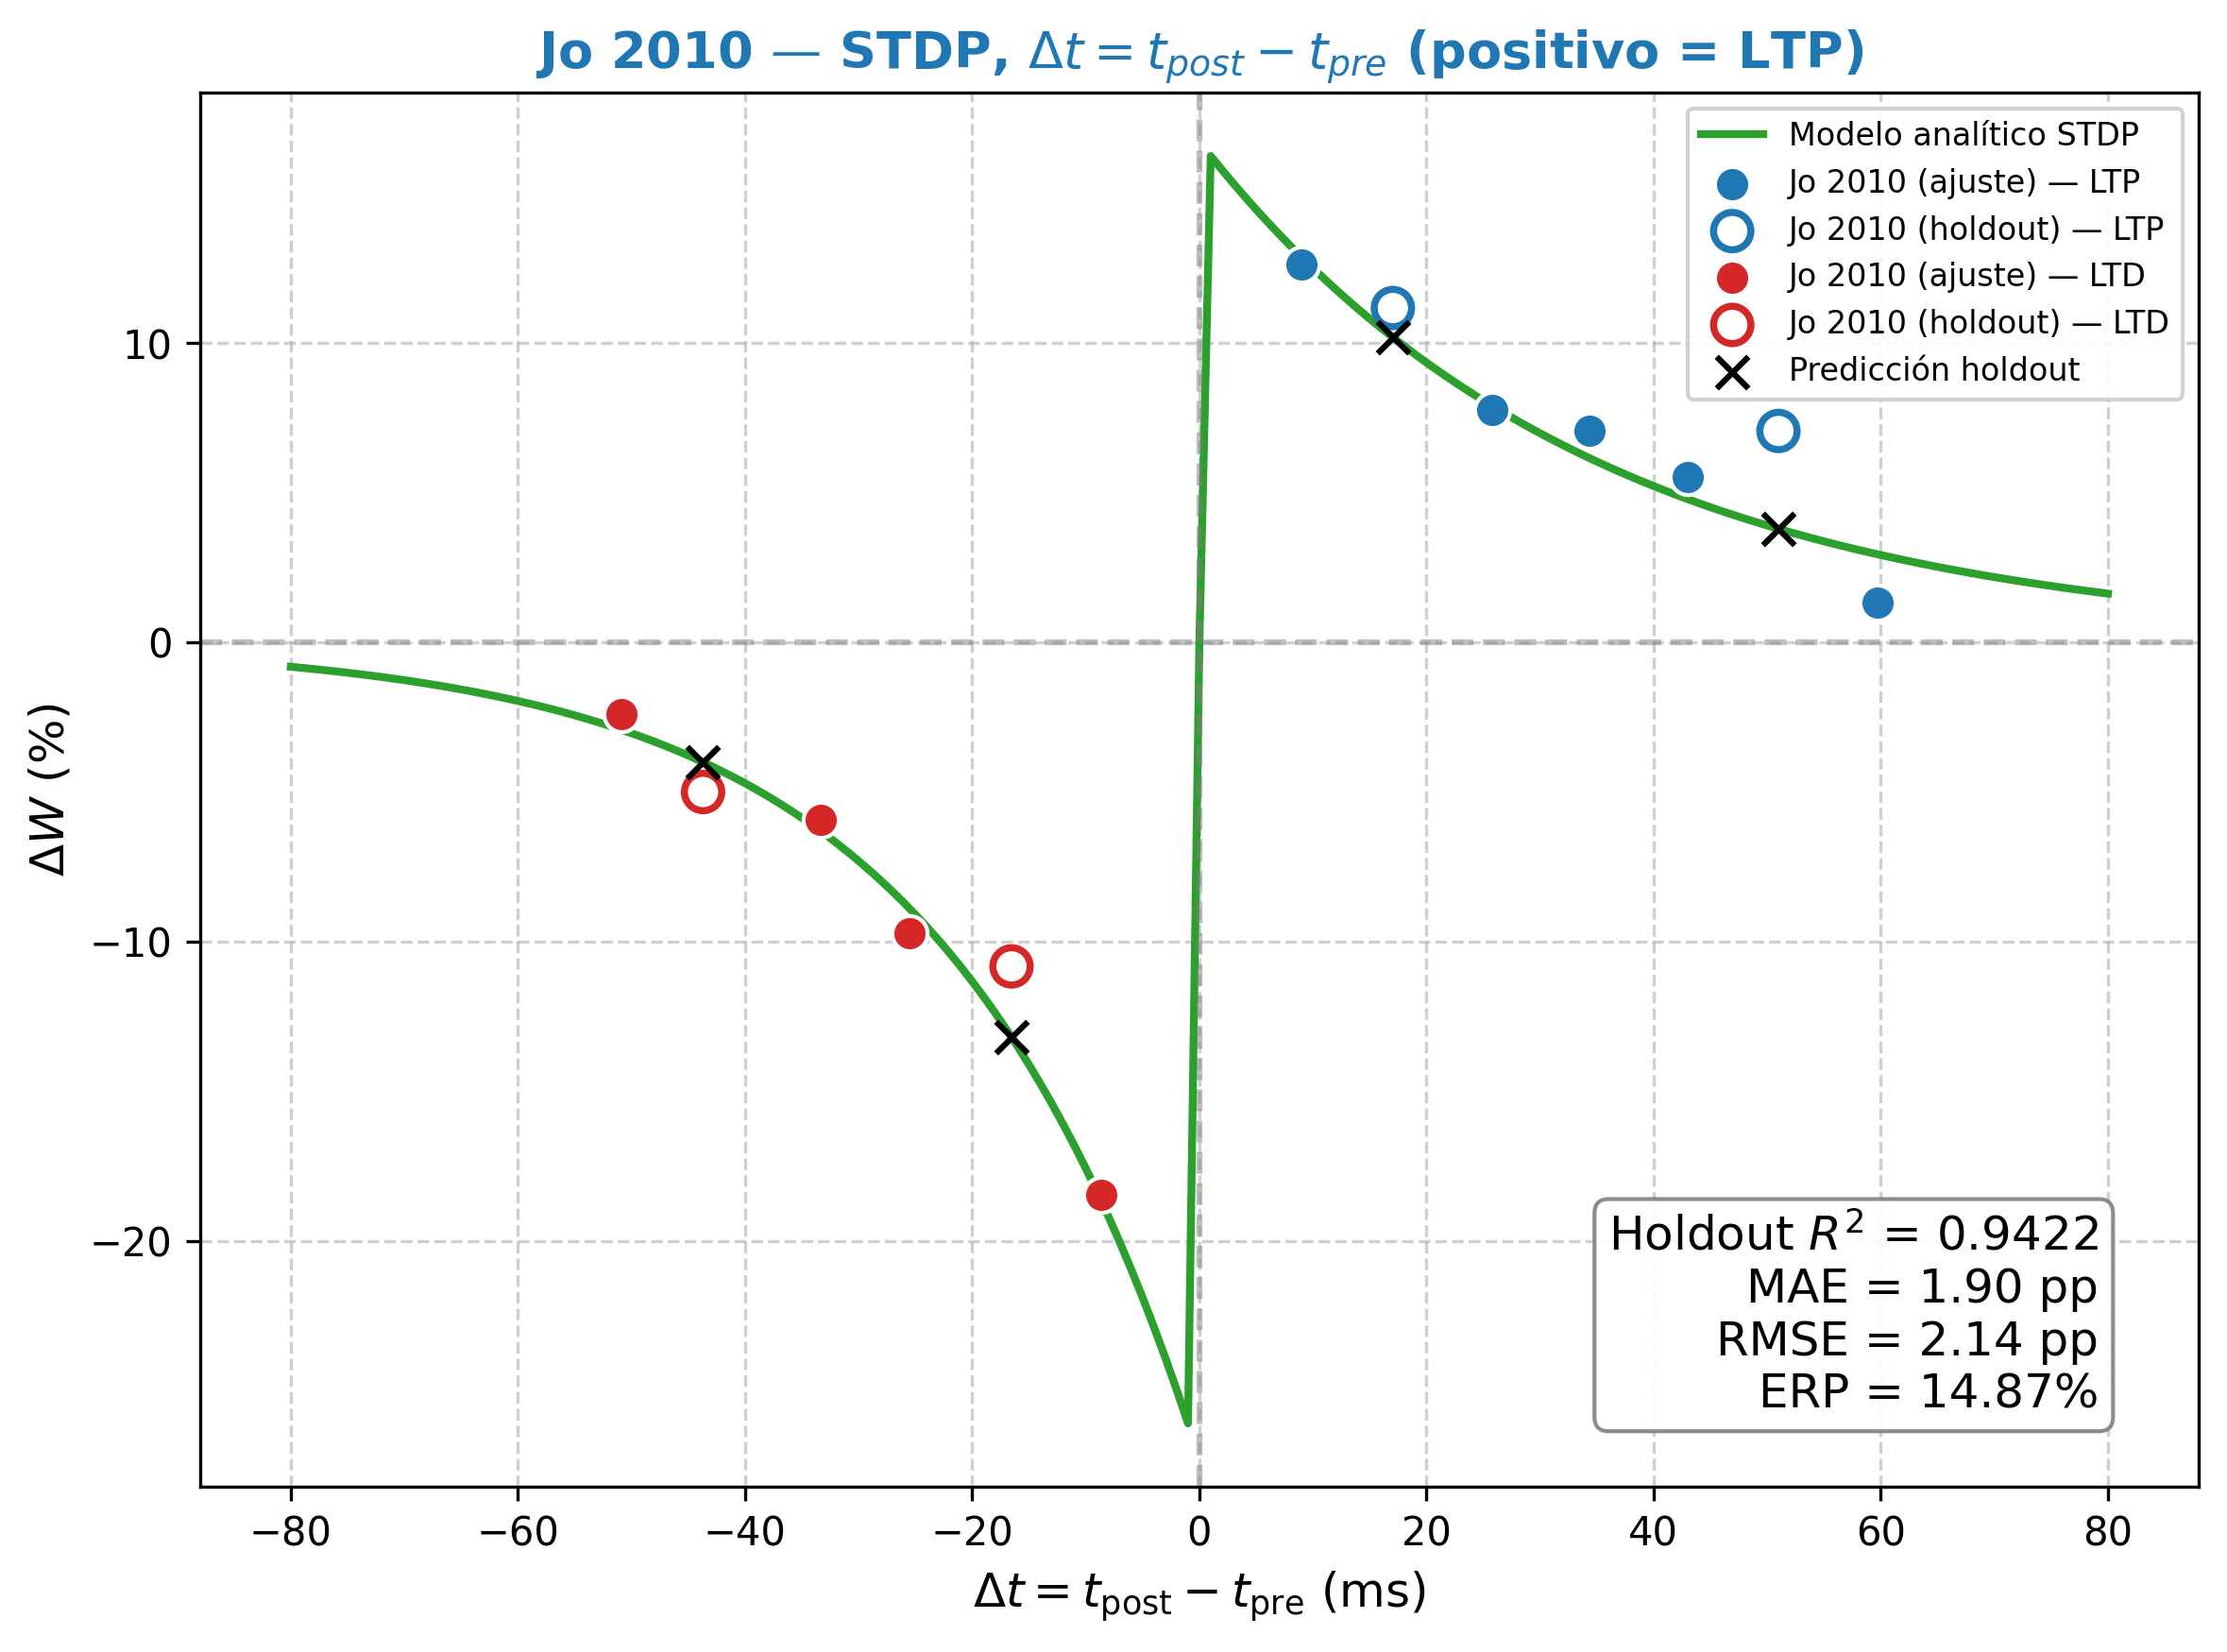
\includegraphics[width=0.72\textwidth]{figuras/fig_15b_stdp_jo2010.png}
\caption{Ajuste STDP en nueve puntos y evaluaci\'on en cuatro puntos reservados atribuidos a Jo et al. (2010).}
\label{fig:stdp_curve_ch3}
\end{figure}
\begin{figure}[H]
\centering
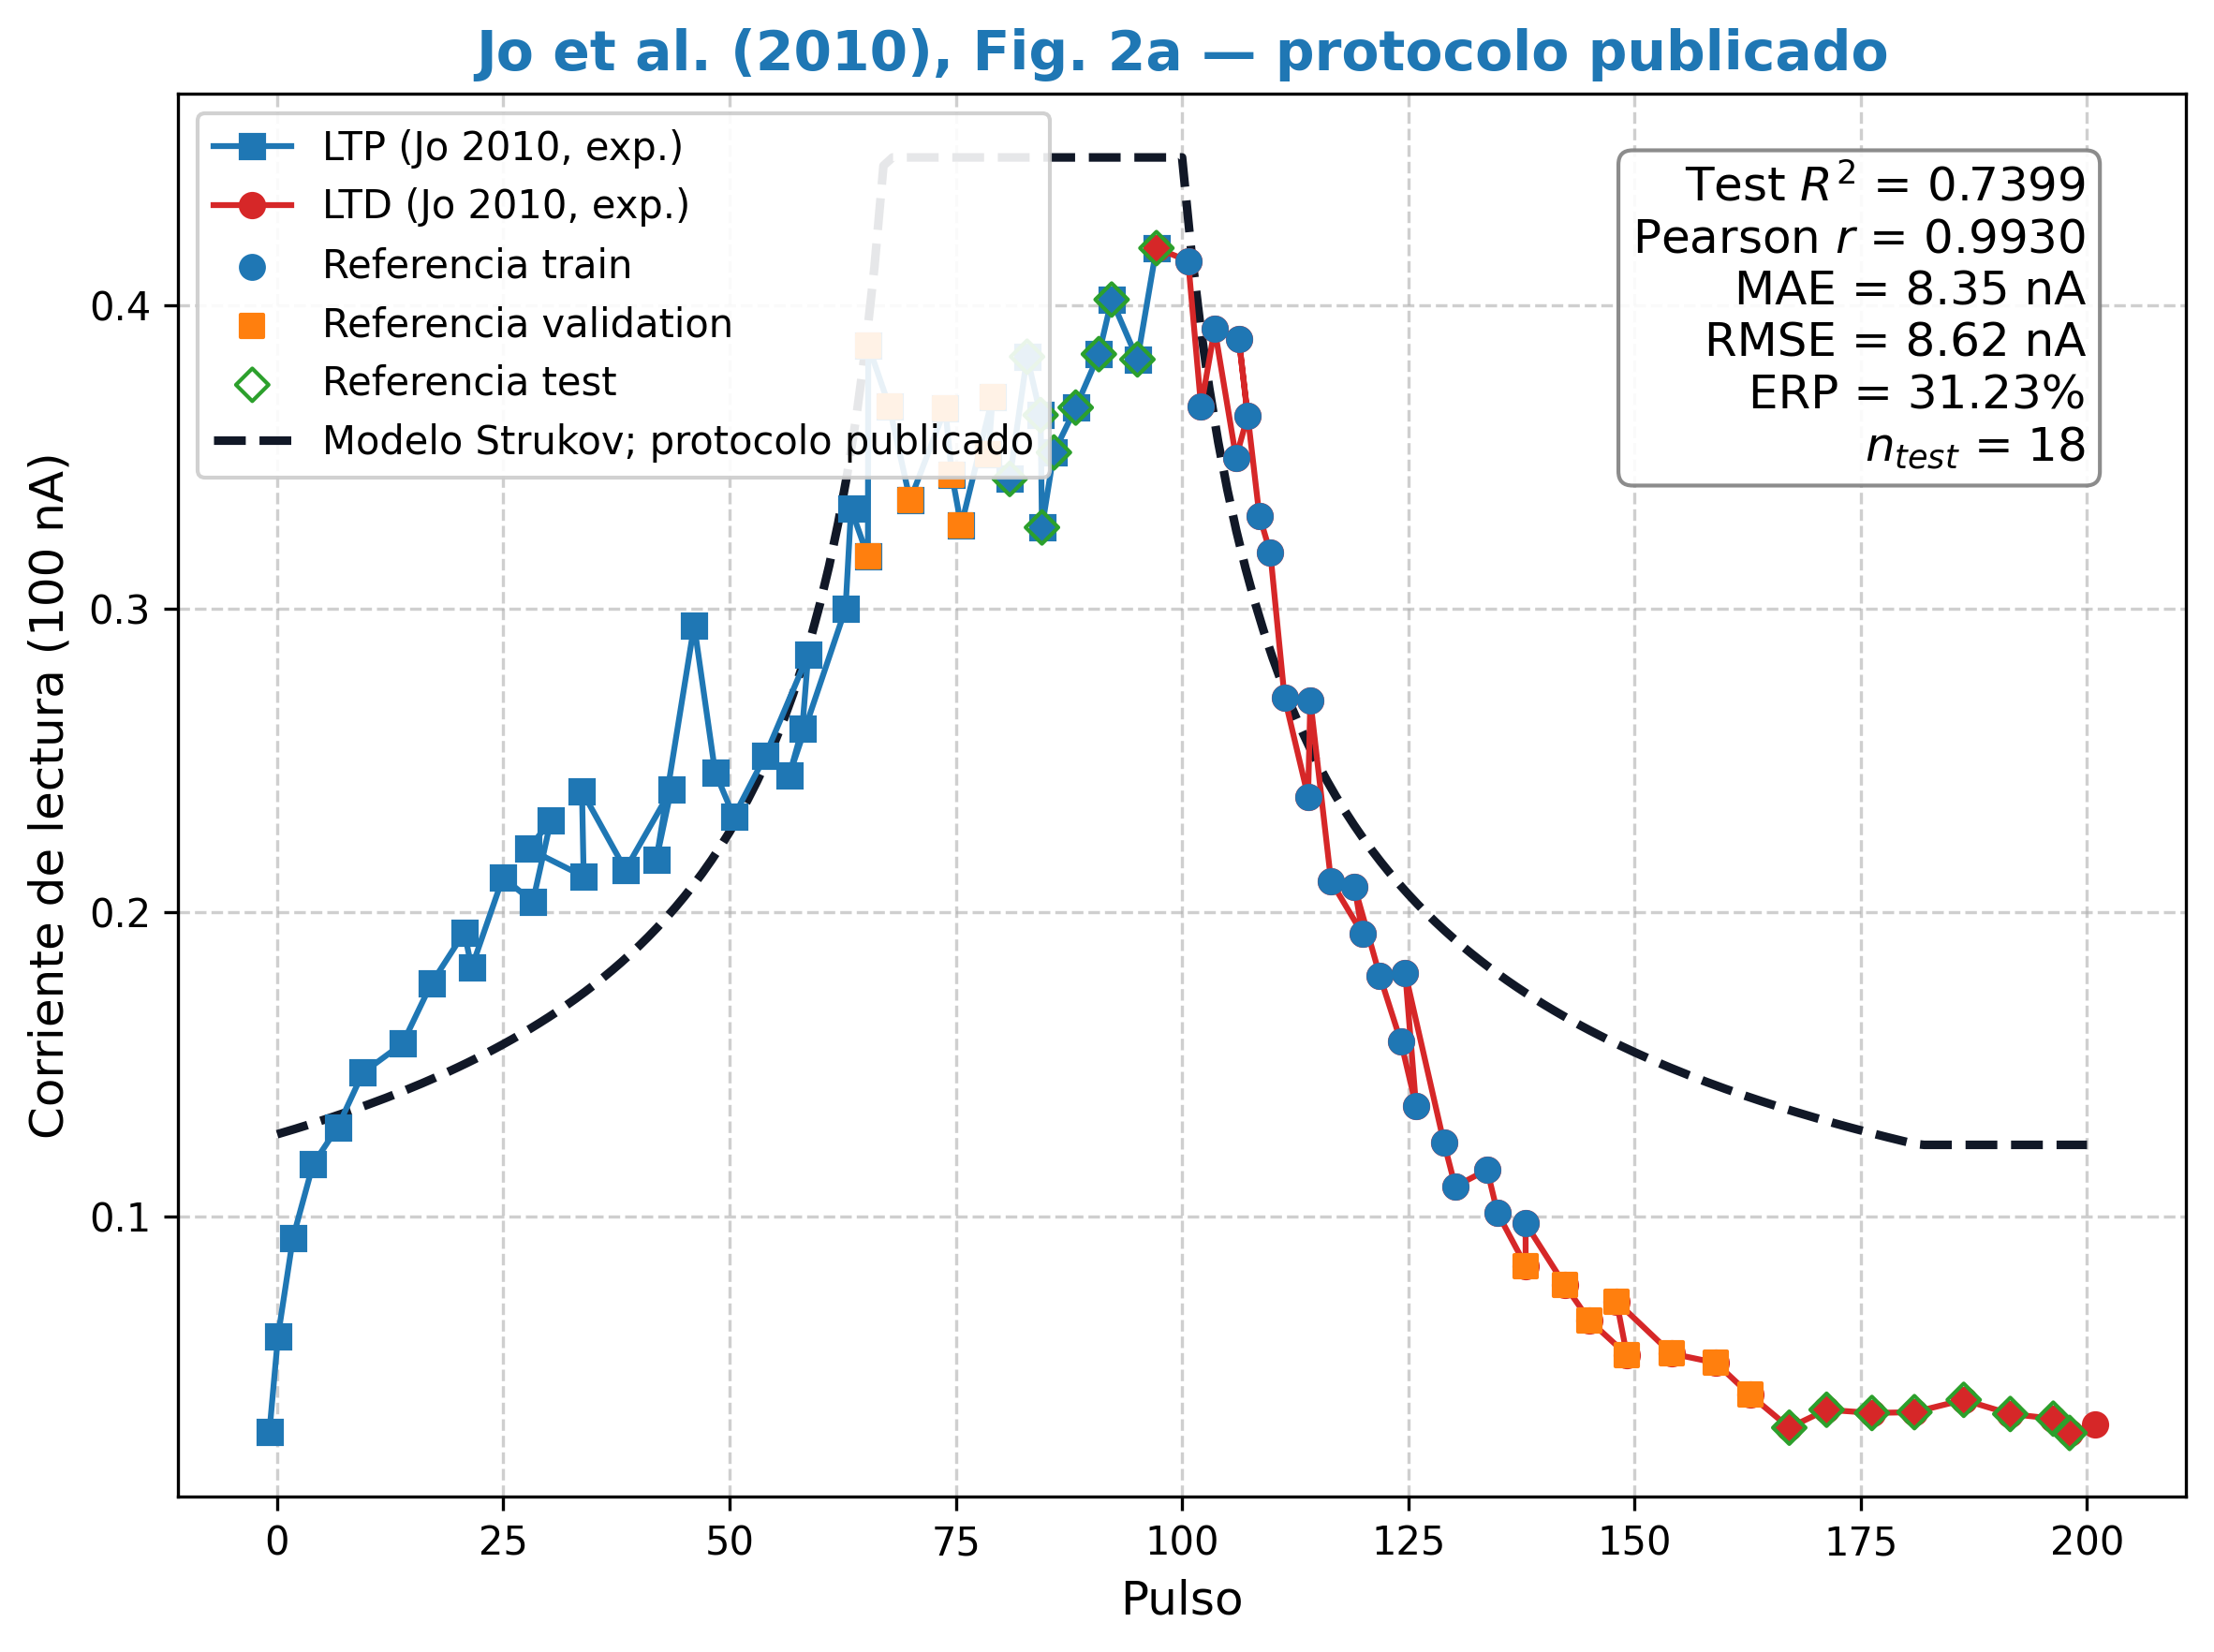
\includegraphics[width=0.72\textwidth]{figuras/fig_14b_ltp_ltd_jo2010.png}
\caption{Comparaci\'on LTP/LTD atribuida a Jo et al. (2010); los par\'ametros se ajustaron con datos de entrenamiento.}
\label{fig:ltp_ltd_curve_ch3}
\end{figure}

\begin{table}[H]
\centering
\small
\caption{Cumplimiento de objetivos seg\'un el alcance de la evidencia.}
\label{tab:cumplimiento_objetivos}
\begin{tabularx}{\textwidth}{l X l}
\toprule
Objetivo & Evidencia resumida & Estado\\
\midrule
Modelos memristivos y variabilidad & Comparaciones digitalizadas y pruebas sint\'eticas; alcance acotado. & Parcial\\
Neurona LIF & Disparo, reinicio, refractario y curva $f-I$ frente a soluci\'on anal\'itica. & Verificado internamente\\
Plasticidad local & STDP con cuatro puntos reservados; conjunto peque\~no. & Parcial\\
Crossbar & Solver MNA y comprobaci\'on num\'erica; sin medici\'on f\'isica. & Verificado en simulaci\'on\\
Aprendizaje de tareas & REINFORCE de referencia y piloto R-STDP con resultados variables. & Parcial\\
\bottomrule
\end{tabularx}
\end{table}

\subsection{Verificaci\'on del sistema integrado}
\label{sec:crossbar_manual}

Se verific\'o la conversi\'on de unidades, un caso manual de crossbar $2\times2$
y la invariancia de pesos durante evaluaciones congeladas. La respuesta LIF
se contrast\'o con la soluci\'on anal\'itica frecuencia--corriente; la prueba
temporal comprueba umbral, reinicio y refractario en el propio modelo. El
Ap\'endice t\'ecnico distingue estas verificaciones de una validaci\'on f\'isica.

La prueba manual usa $G=[[0.001,0.0005],[0.00033333,0.00025]]\,\mathrm{S}$ y
$V=[0.05,0]^{\mathsf T}\,\mathrm{V}$. La multiplicaci\'on ideal produce
$[50,25]~\mu\mathrm{A}$; el solver MNA produce $[44.1176,23.2558]~\mu\mathrm{A}$.
La diferencia corresponde a las resistencias del protocolo del solver, no a
la identidad matricial ideal.

\begin{figure}[H]
\centering
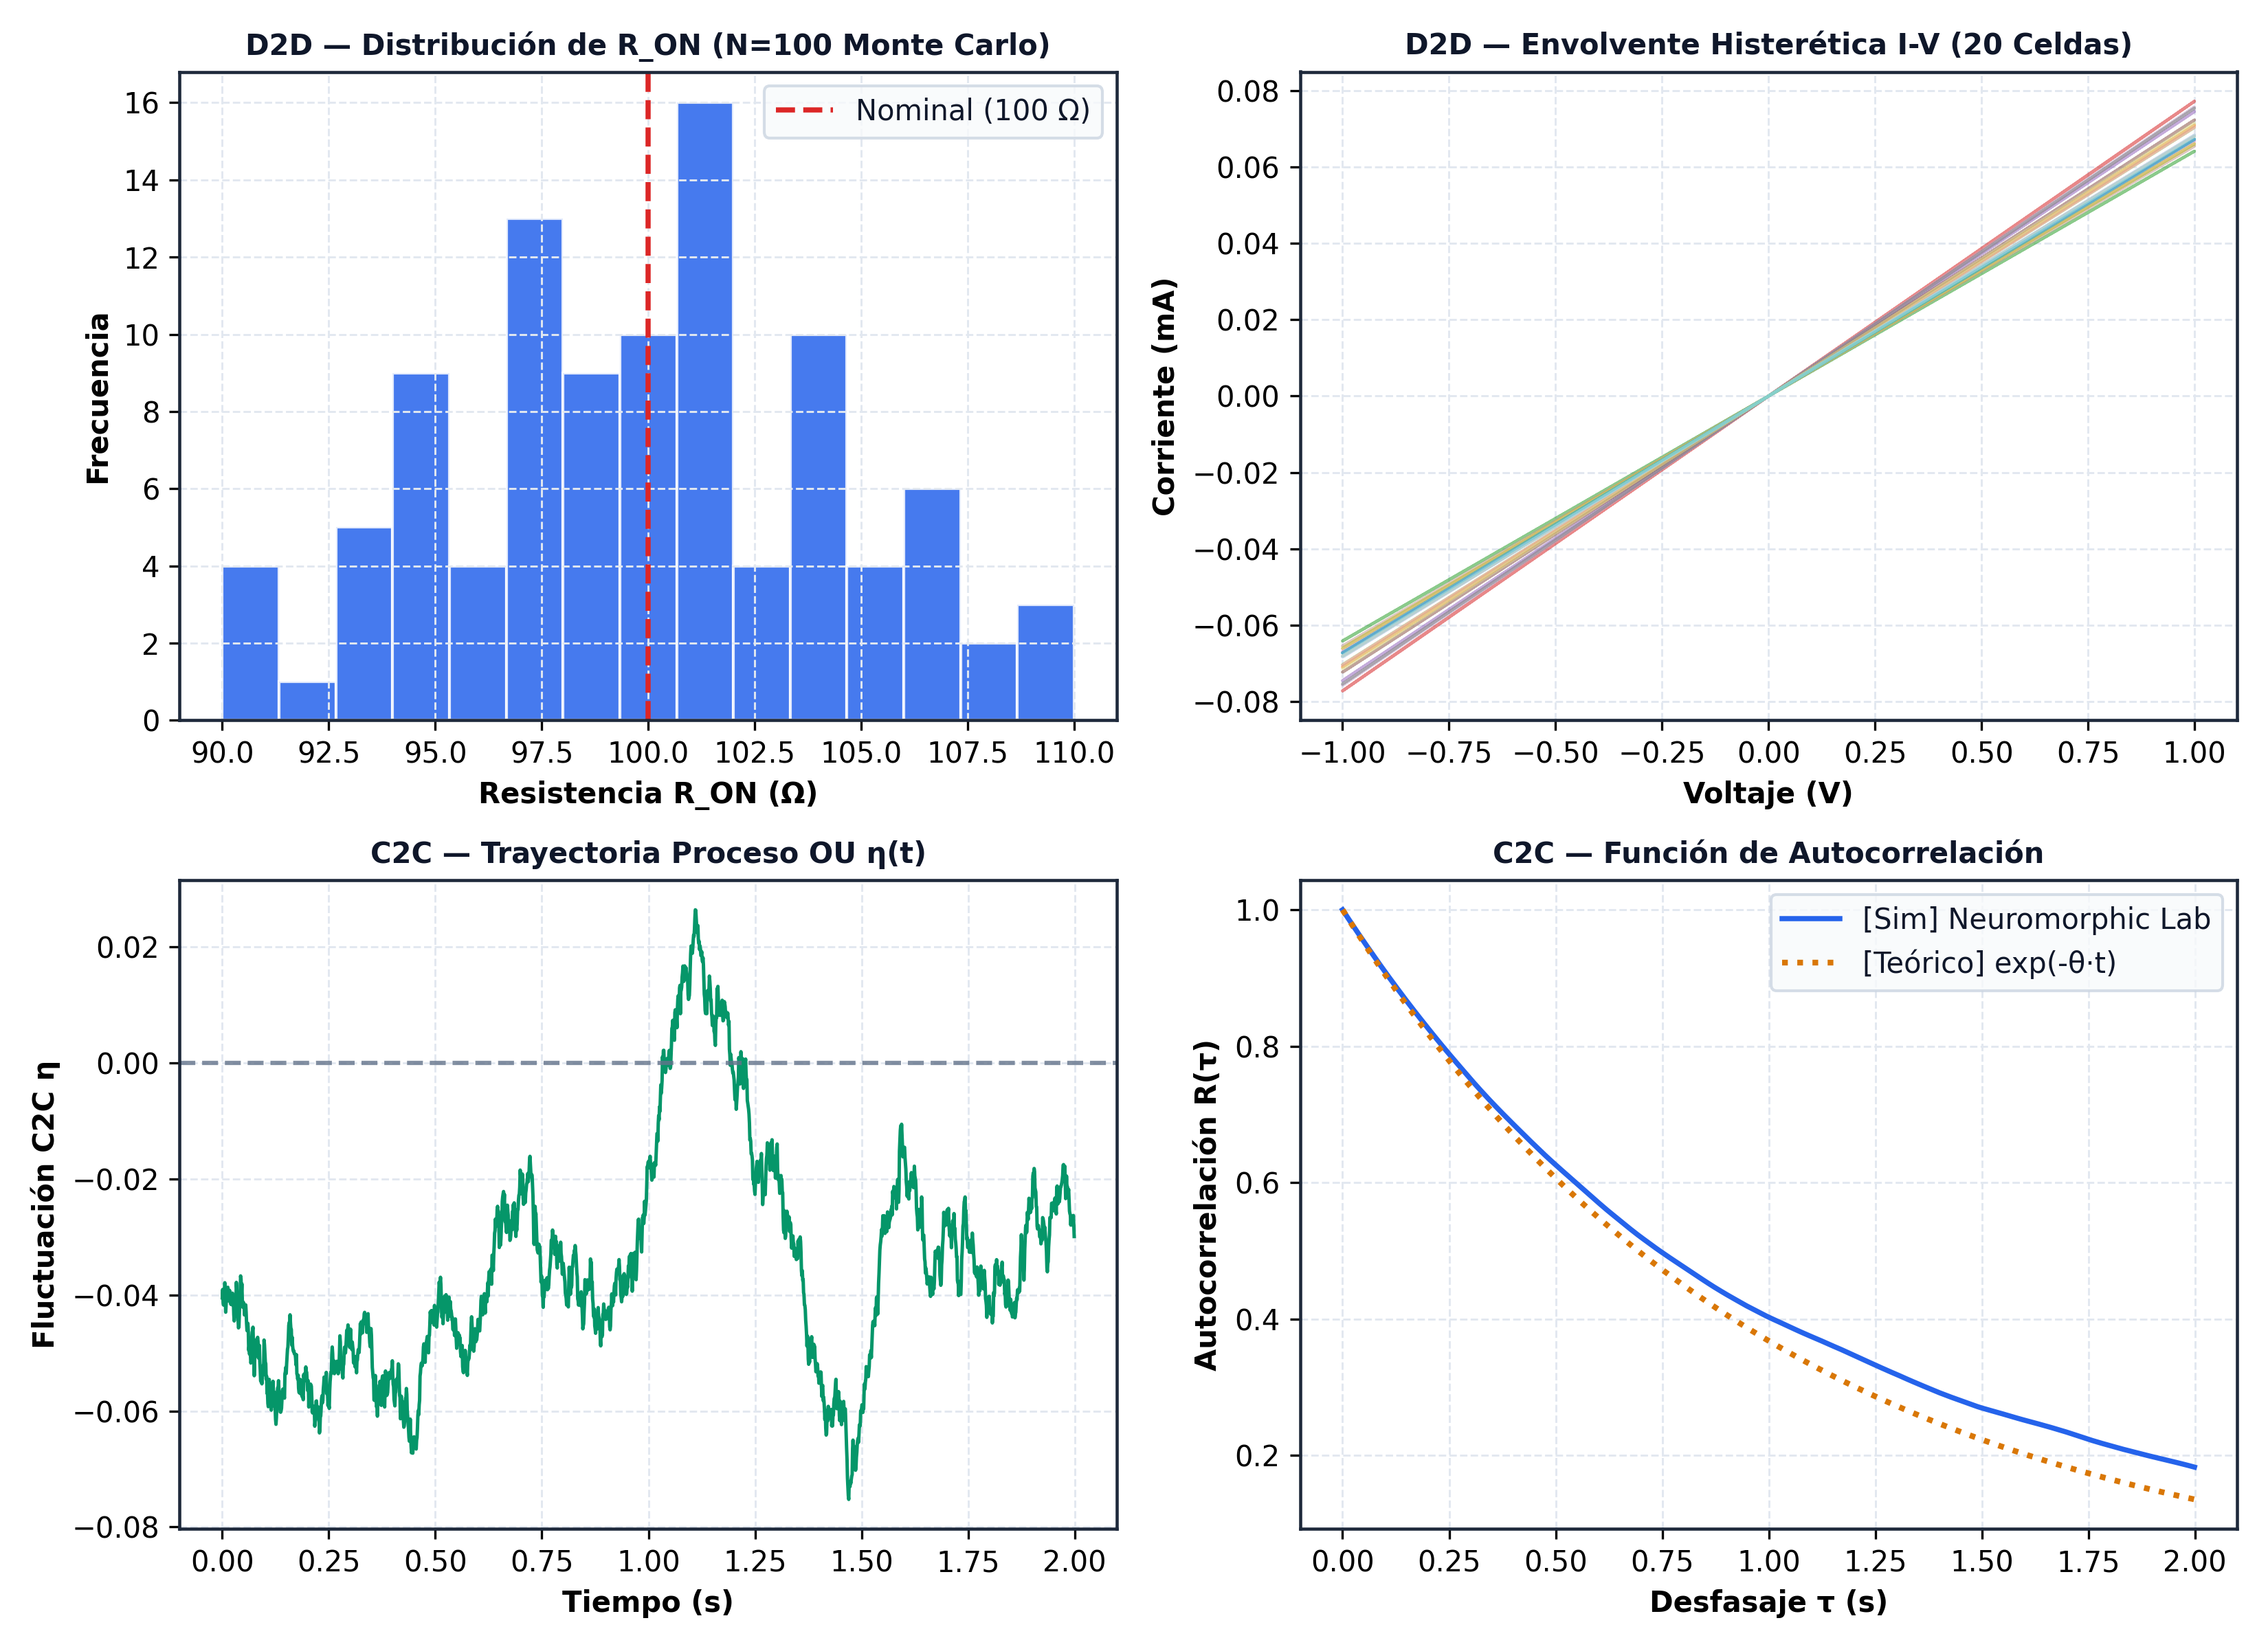
\includegraphics[width=0.67\textwidth]{figuras/fig_05_d2d_c2c.png}
\caption{Distribuciones sint\'eticas D2D/C2C del modelo y sus referencias te\'oricas; no son histogramas de mediciones f\'isicas.}
\label{fig:d2d_c2c_validation}
\end{figure}

\begin{figure}[H]
\centering
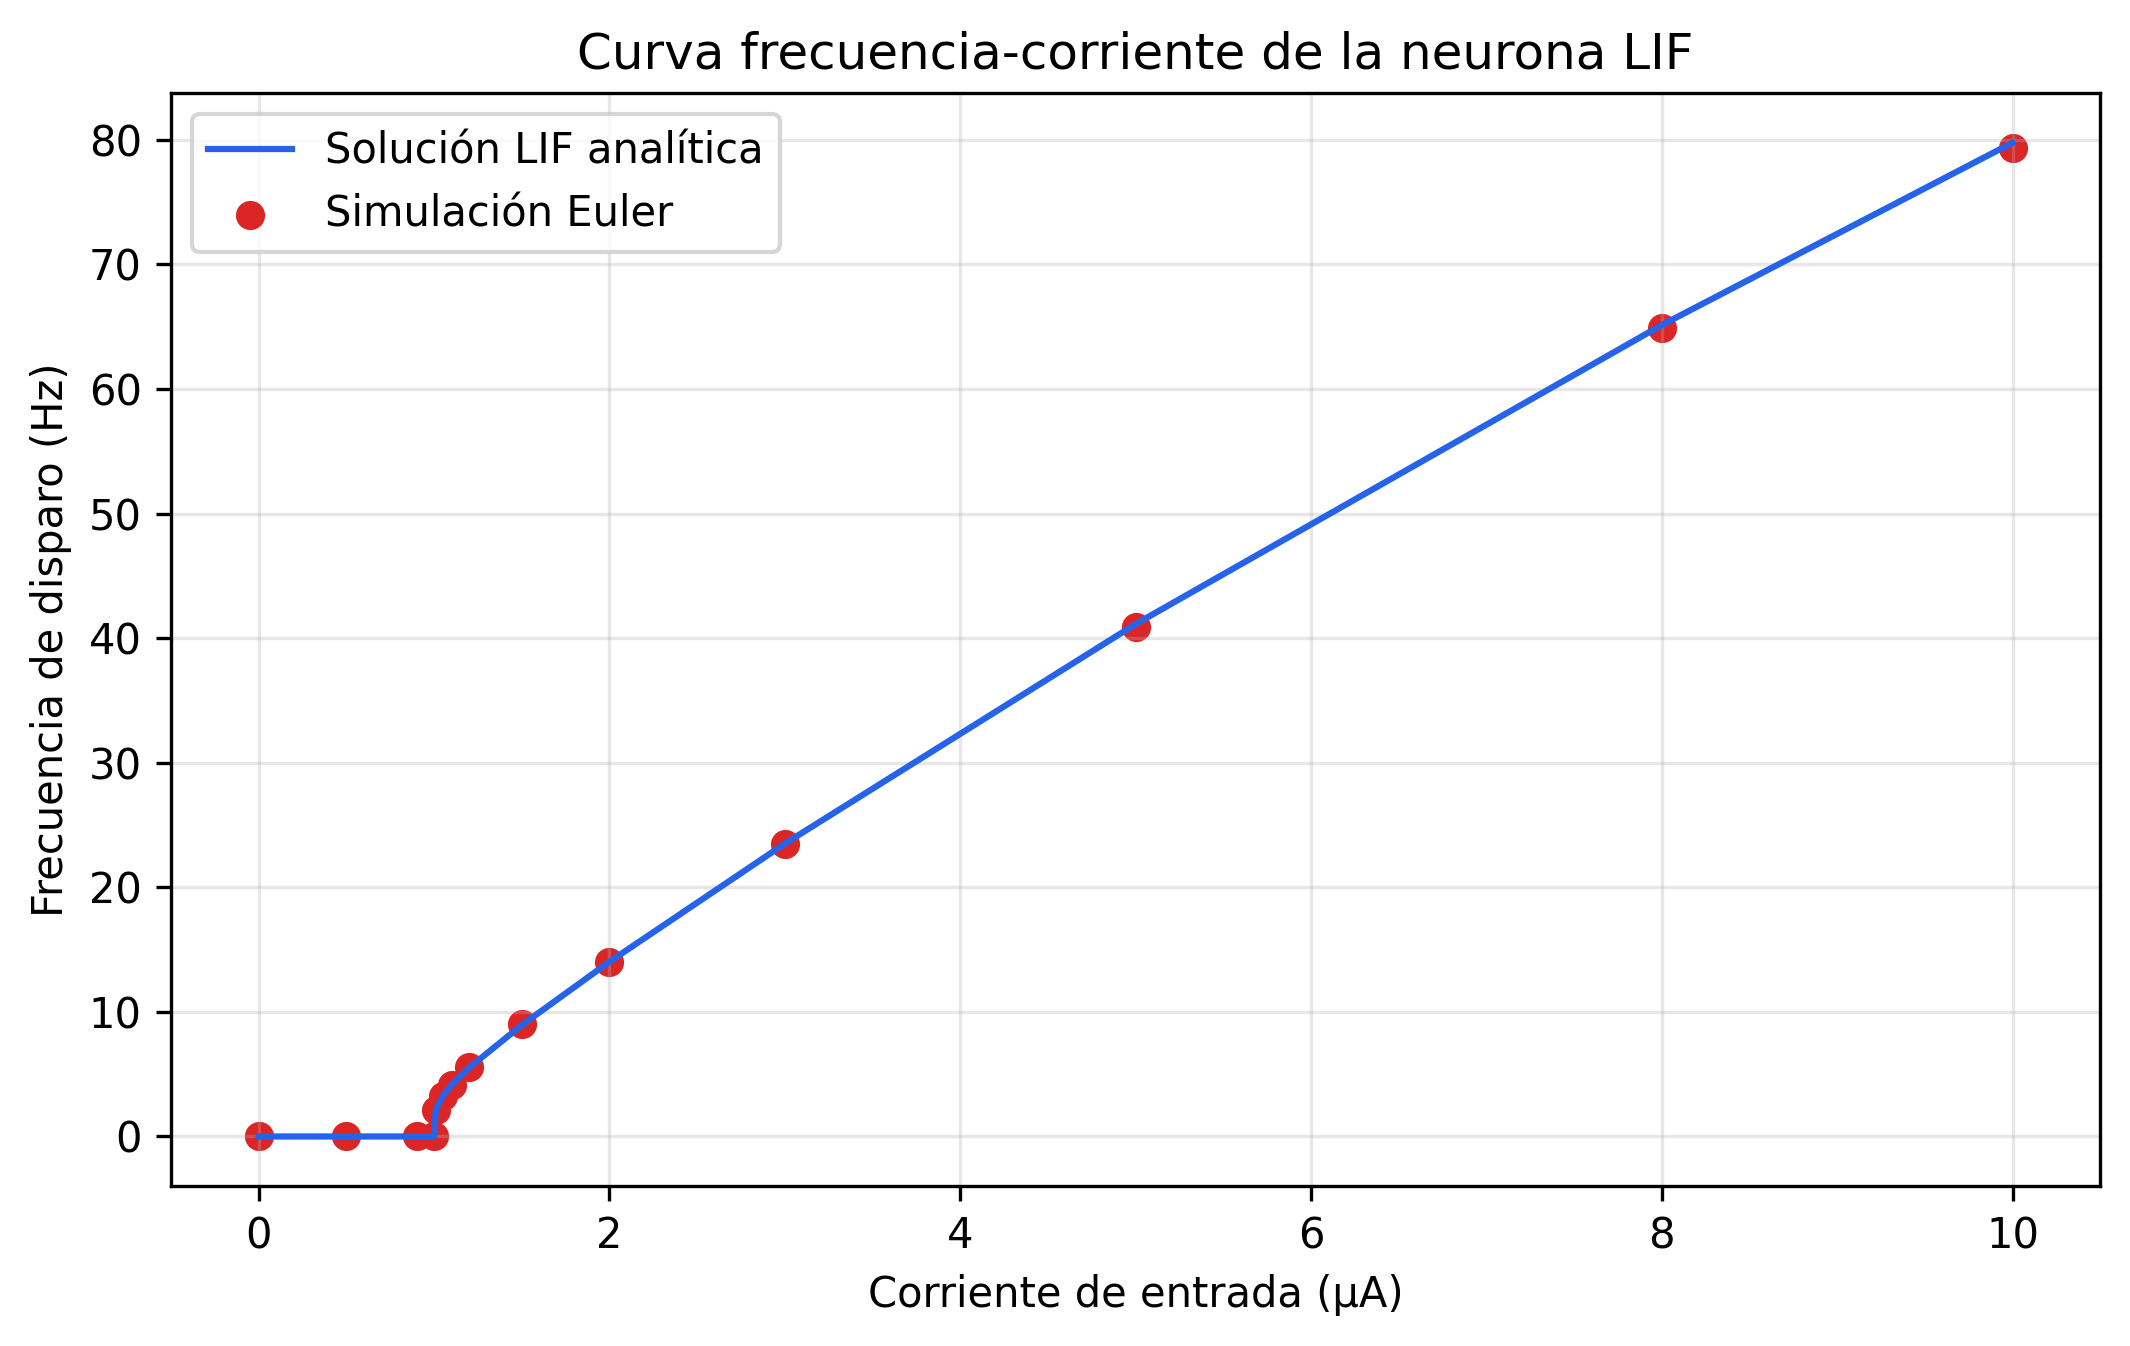
\includegraphics[width=0.67\textwidth]{figuras/lif_fi_curve.png}
\caption{Frecuencia de disparo LIF por Euler frente a la soluci\'on anal\'itica del mismo modelo.}
\label{fig:lif_fi_curve}
\end{figure}

\section{Resultados y discusi\'on}
\label{sec:resultados}

Las m\'etricas de cada aplicaci\'on son espec\'ificas y no se interpretan como
comparaci\'on controlada cuando cambian la arquitectura, la recompensa o el
presupuesto de entrenamiento. Los registros y matrices por condici\'on est\'an
en el Ap\'endice~\ref{ap:evidencia_entrenamientos}.


\begin{table}[H]
\centering
\scriptsize
\setlength{\tabcolsep}{3pt}
\caption{Separaci\'on de entrenamiento, validaci\'on y test en las aplicaciones.}
\label{tab:train_validation_test_tasks}
\begin{tabularx}{\textwidth}{l X X X}
\toprule
Tarea & Entrenamiento & Validaci\'on y selecci\'on & Test independiente\\
\midrule
CartPole & Cinco semillas, 300 episodios cada una. & 50 episodios por checkpoint; se selecciona semilla 4 ($493.77$). & 50 episodios, semillas 20000--20049; $493.63\pm0.93$.\\
Visi\'on & Tres semillas, 5000 episodios sobre ocho plantillas. & 160 variantes por checkpoint con inversi\'on de p\'ixel $p=0.05$; selecci\'on: semilla 2 ($42.5\%$). & 400 variantes nuevas; exactitud $42.5\%$.\\
Obst\'aculos & Semillas 0--2; 746, 800 y 800 episodios. & 20 mapas por checkpoint; selecci\'on: semilla 2 ($25\%$). & 50 mapas nuevos; \'exito $4\%$ (2/50).\\
Auto 2D & Una semilla; horizonte reportado de 3000 episodios y snapshots cada 200. & 20 escenarios por snapshot; checkpoint reportado con $15\%$. & 50 escenarios; \'exito reportado $14\%$ (7/50); faltan logs para recalcular.\\
\bottomrule
\end{tabularx}
\end{table}

\subsection{CartPole-v1: control con recompensa densa}
\label{sec:res_cartpole}

Se entren\'o el agente $24\times12$ durante 300 episodios en cinco semillas,
con D2D/C2C y supresi\'on de actualizaci\'on en cada episodio cuya recompensa
alcanz\'o 430. La recompensa media de los \'ultimos 200 episodios fue 369.66,
421.44, 474.31, 462.79 y 448.36 para las semillas 0--4 (media $435.31$,
desviaci\'on est\'andar $37.28$). Cuatro corridas alcanzaron una recompensa
epis\'odica de 480. El umbral omite una actualizaci\'on de pesos de ese episodio,
pero no congela permanentemente el agente.

Para evaluar dentro de la tarea, se seleccion\'o en validaci\'on el checkpoint
de la semilla 4 y se evalu\'o sin aprendizaje en 50 episodios de test
independientes. Obtuvo $493.63\pm0.93$ puntos (rango 490.43--494.94);
$X$ no cambi\'o y el decoder fue greedy. En la comparaci\'on emparejada
ideal--D2D/C2C, la diferencia media fue $+99.46\pm226.90$ puntos, pero
solo tres de cinco pares favorecieron la condici\'on variable; el resultado
es descriptivo y no prueba una ventaja general. La curva de cinco semillas
est\'a en la Figura~\ref{fig:cartpole_learning}.

\begin{figure}[H]
\centering
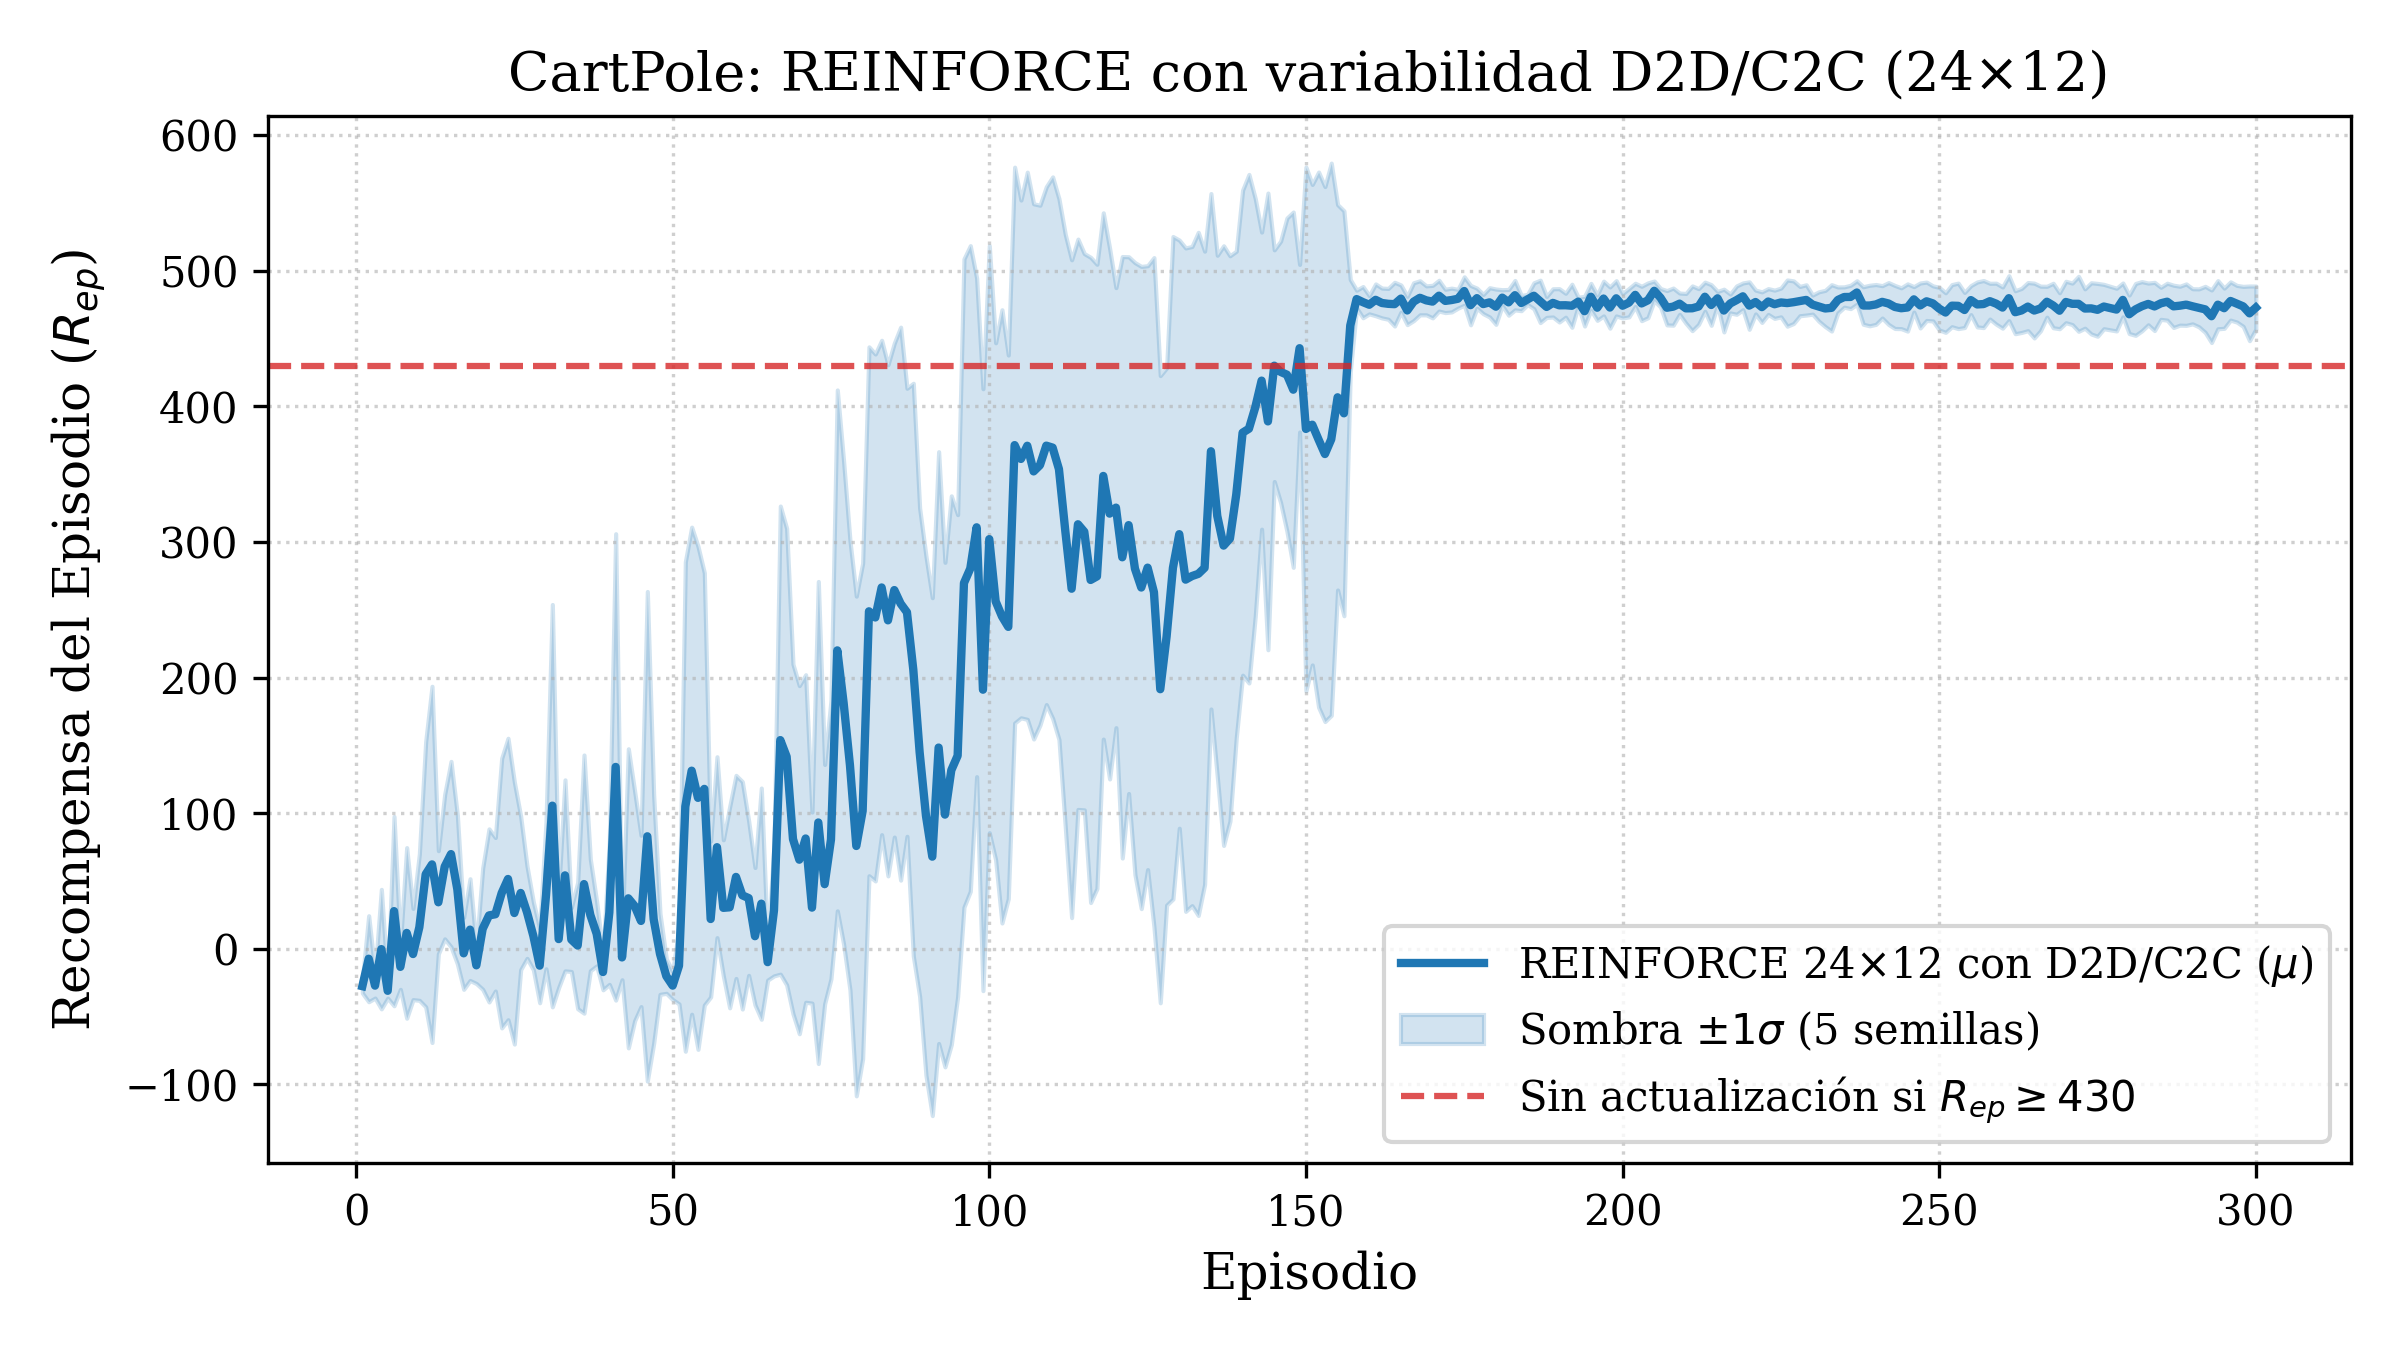
\includegraphics[width=0.76\textwidth]{figuras/cartpole_learning_24x12_5seeds_d2d_c2c.png}
\caption{Recompensa de cinco corridas CartPole con D2D/C2C, suavizada para facilitar la lectura.}
\label{fig:cartpole_learning}
\end{figure}

\subsection{Visi\'on $8\times8$: clasificaci\'on supervisada}
\label{sec:res_vision}

La tarea clasific\'o ocho patrones binarios mediante un crossbar $64\times8$.
En tres corridas de 5000 episodios, el acierto de los \'ultimos 200 episodios
fue 100\%. Ese dato corresponde a las ocho plantillas del entrenamiento.
Para medir robustez se reservaron variantes con inversi\'on de p\'ixeles; tras
selecci\'on por validaci\'on, la semilla 2 obtuvo 42.5\% sobre 400 variantes
de test, frente a 12.5\% aleatorio. El test mide ruido sint\'etico sobre las
plantillas, no clases ni im\'agenes externas.

\begin{figure}[H]
\centering
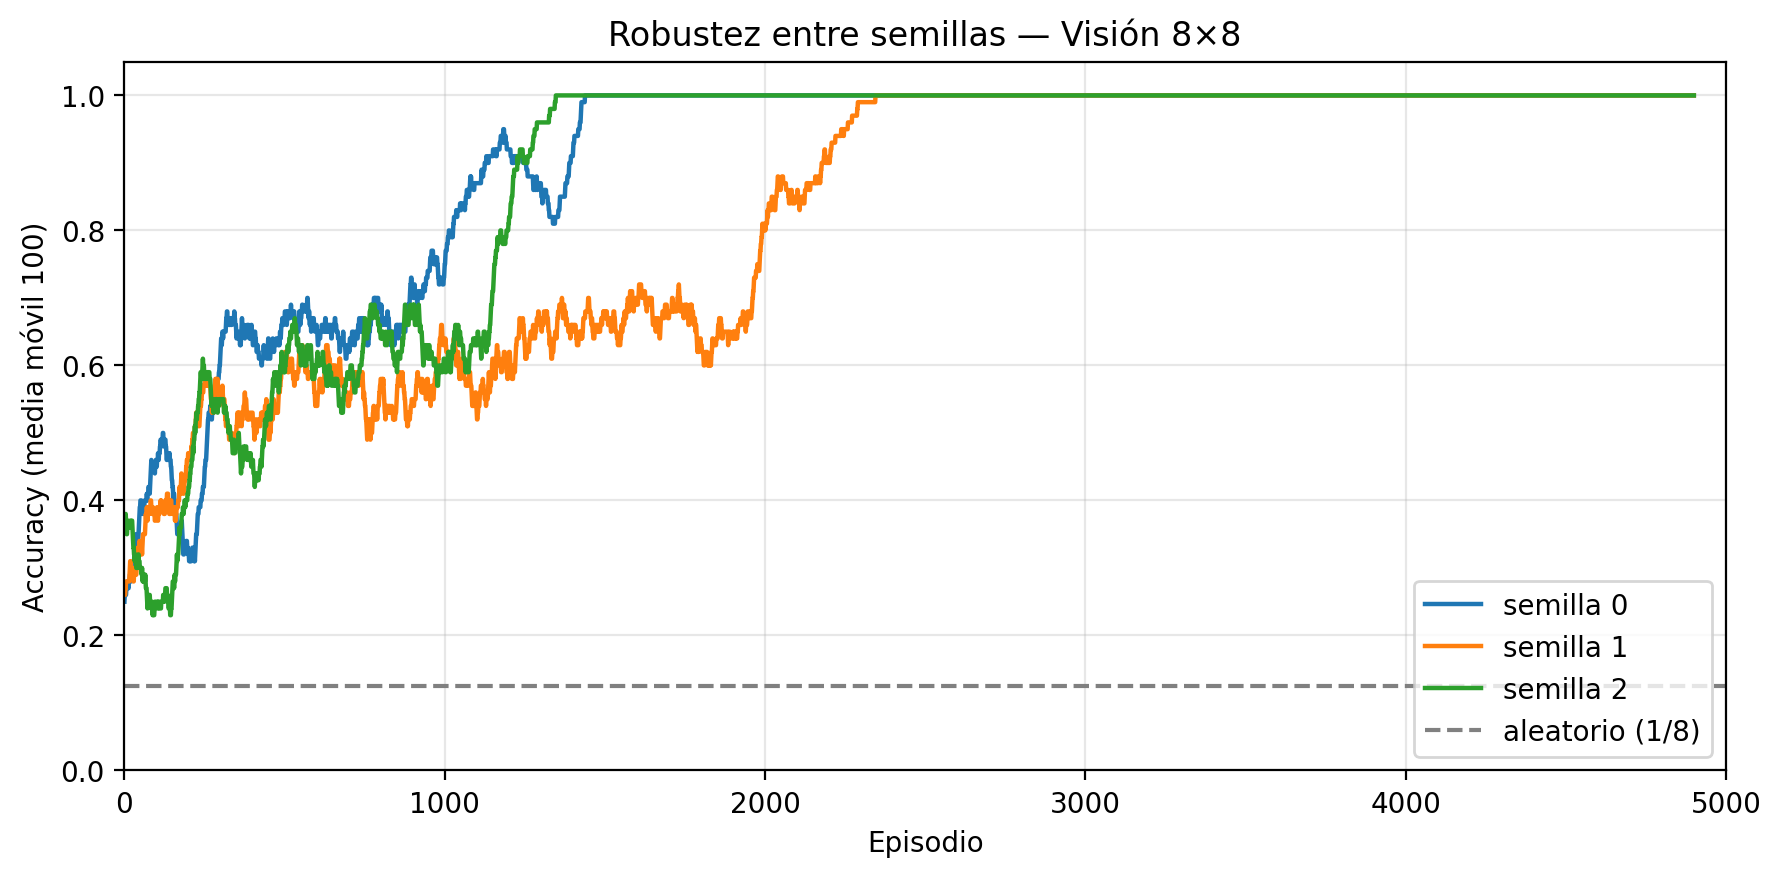
\includegraphics[width=0.72\textwidth]{figuras/vision_seeds.png}
\caption{Exactitud de tres corridas de visi\'on, suavizada con una ventana de 100 episodios.}
\label{fig:vision_seeds}
\end{figure}

\subsection{Navegaci\'on $10\times10$: control con recompensa escasa}
\label{sec:res_navegacion}

El gridworld contiene 15 obst\'aculos y cuatro movimientos, con recompensa
por llegar a la meta y penalizaciones por paso y colisi\'on. Las tasas de
\'exito de los \'ultimos 200 episodios fueron 100\%, 49.5\% y 82\% (media
no ponderada 77.17\%). En 50 mapas nuevos, el checkpoint seleccionado en
validaci\'on alcanz\'o la meta en 2 mapas (4\%). El buen resultado en el mapa
de entrenamiento no se transfiri\'o a mapas distintos en esta prueba. Los
registros de esa evaluaci\'on no est\'an incluidos como JSON recalculable y el
4\% se identifica como resultado reportado.

\begin{figure}[H]
\centering
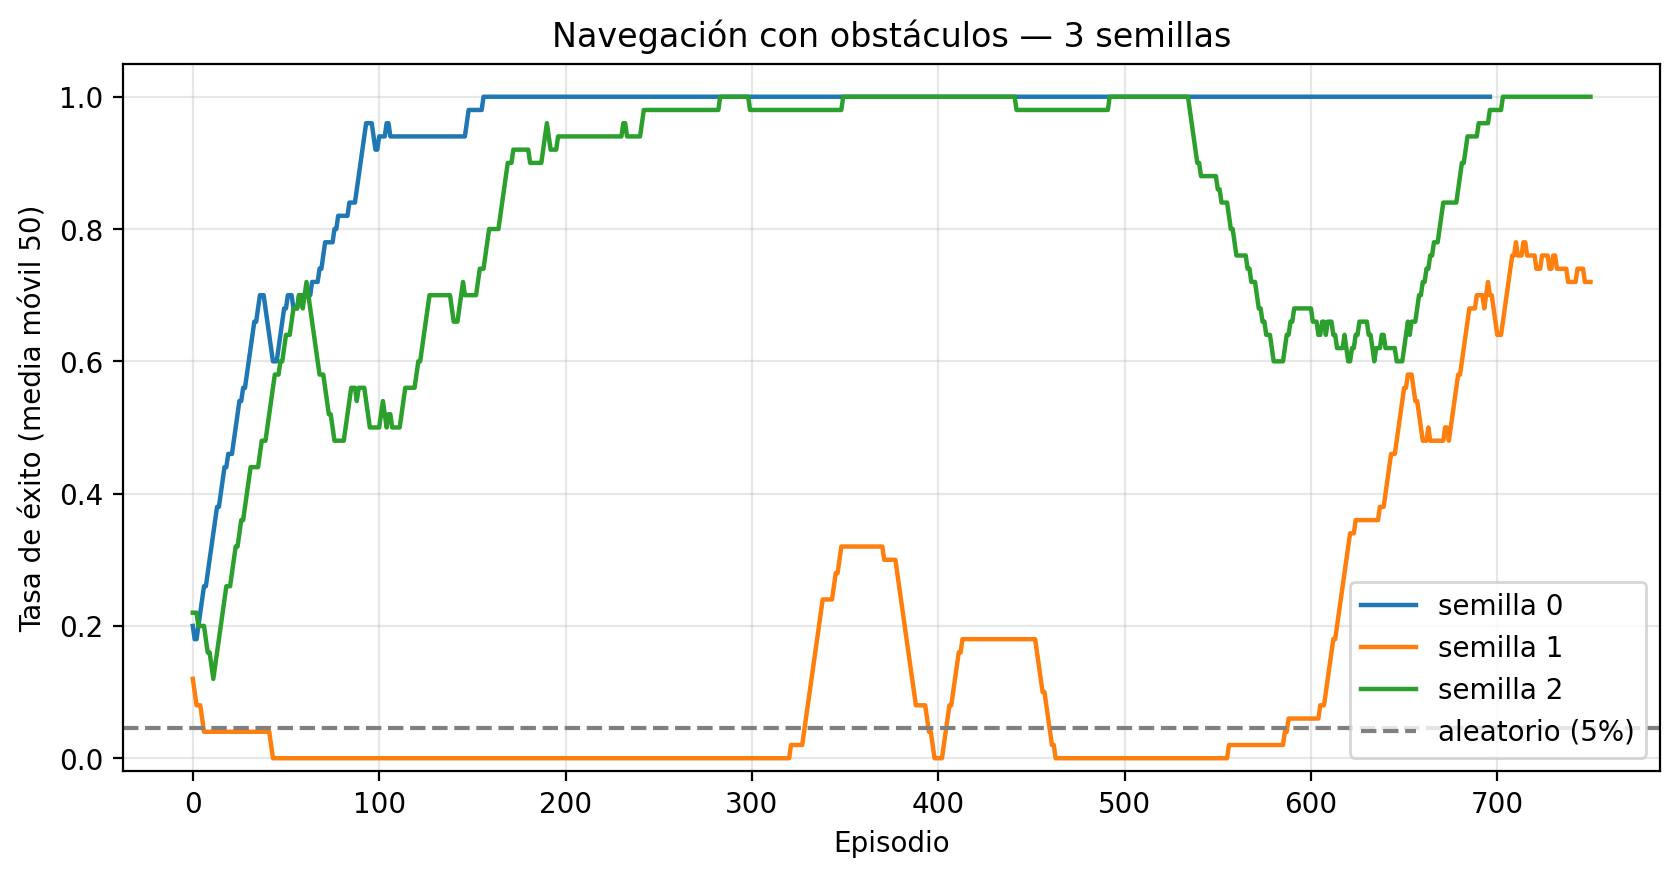
\includegraphics[width=0.72\textwidth]{figuras/obstacle_learning.png}
\caption{Tasa de \'exito de tres corridas del gridworld, suavizada con una ventana de 50 episodios.}
\label{fig:obstacle_learning}
\end{figure}

\subsection{Auto 2D: entorno continuo de conducci\'on}
\label{sec:res_auto2d}

El entorno combina ocho sensores de distancia, direcci\'on y cuatro controles,
con crossbar $24\times8$. El registro disponible indica 5.0\% de \'exito en
los \'ultimos 200 episodios; una evaluaci\'on reportada obtuvo 14\% (7/50) en
test. Solo existe una semilla y faltan los archivos necesarios para
reconstruir la curva y el checkpoint evaluado. Se considera un resultado
piloto, no evidencia de robustez entre semillas.

\subsection{An\'alisis comparativo entre tareas}
\label{sec:comparativa}
\label{sec:interpretacion_comparativa}

La Tabla~\ref{tab:cross_task} resume los \'ultimos 200 episodios de los
registros de presupuesto fijo. Recompensa, exactitud y tasa de llegada
son magnitudes diferentes; adem\'as, las tareas usan matrices y protocolos
distintos. La comparaci\'on es descriptiva y no estima un efecto causal de
la arquitectura ni de la regla de aprendizaje.

\begin{table}[H]
\centering
\small
\caption{Resumen descriptivo de las corridas de presupuesto fijo.}
\label{tab:cross_task}
\begin{tabular}{lccccc}
\toprule
Tarea & Episodios & Semillas & M\'etrica final & $\bar X$ & $\sigma_X$\\
\midrule
CartPole & 300 & 5 & $\bar R_{200}=435.31$ & 0.1379 & 0.0717\\
Visi\'on $8\times8$ & 5000 & 3 & $\mathrm{Acc}_{200}=100\%$ & $\approx0.10$ & 0.022--0.030\\
Navegaci\'on & 746--800 & 3 & $S_{200}=77.17\%$ & 0.221--0.345 & 0.190--0.288\\
Auto 2D & 1000 & 1 & $S_{200}=5.0\%$ & 0.319 & 0.274\\
\bottomrule
\end{tabular}
\end{table}

\subsection{Piloto comparativo REINFORCE/R-STDP}
\label{sec:piloto_rstdp_reinforce}

El lote de parada por \'exito evalu\'o CartPole, visi\'on y obst\'aculos con ambos
algoritmos, semillas 0 y 1 e inicializaciones $X_0=0.1$ y $X_0=0.9$.
Car se ejecut\'o solo con R-STDP. El criterio fue al menos 271 \'exitos dentro
de los \'ultimos 300 episodios (90.33\%), con m\'aximo de 10\,000 episodios;
no exige 300 \'exitos consecutivos. Cada tarea conserva su tama\~no de crossbar
y definici\'on de \'exito. La tabla resume los registros del piloto.

\begin{table}[H]
\centering
\footnotesize
\begin{tabularx}{\textwidth}{l l p{1.5cm} X}
\toprule
Tarea & Regla & Criterio & Episodios / alcance\\
\midrule
CartPole & REINFORCE & 2/4 & 349 y 1249; dos registros incompletos a 559 y 1132.\\
CartPole & R-STDP & 4/4 & 307--1199 episodios.\\
Visi\'on & REINFORCE & 4/4 & 586--1357 episodios.\\
Visi\'on & R-STDP & 4/4 & 470--2951 episodios.\\
Obst\'aculos & REINFORCE & 4/4 & 300 episodios en las cuatro condiciones.\\
Obst\'aculos & R-STDP & 4/4 & 300--336 episodios.\\
Car, lote principal & R-STDP & 1/4 & Una condici\'on a 3775; tres a 10\,000 sin criterio.\\
Car, repetici\'on corregida & R-STDP & 2/4 & Semilla 2: 750 y 1548; semilla 4: ambas a 10\,000 sin criterio.\\
\bottomrule
\end{tabularx}
\caption{Resultado del piloto de parada por \'exito. Cada fracci\'on corresponde a cuatro condiciones semilla--$X_0$, salvo donde se indica el alcance incompleto.}
\label{tab:piloto_rstdp_reinforce}
\end{table}

R-STDP designa el modo implementado en el runner: elegibilidad local
modulada por retorno. La regla STDP local del crossbar s\'i produce cambios;
el piloto muestra que su integraci\'on con la tarea todav\'ia es inestable entre
condiciones y dominios. No se extrapola a hardware. La discusi\'on del evento
post, el baseline y la estabilidad est\'a en el Ap\'endice~\ref{ap:desarrollo_extendido}.

\subsection{Limitaciones}
\label{sec:limitaciones}

Los resultados son de simulaci\'on y no se dispone de un prototipo f\'isico.
Las comparaciones con art\'iculos usan datos digitalizados, a veces con pocos
puntos o protocolos incompletos; las pruebas sint\'eticas no sustituyen
mediciones. Las aplicaciones no comparten una m\'etrica ni un protocolo
id\'enticos. Visi\'on se evalu\'o con variantes de plantillas, navegaci\'on mostr\'o
baja transferencia a mapas nuevos y Auto 2D cuenta con una semilla y
archivos incompletos. El piloto R-STDP alcanza el criterio en algunas
condiciones, pero no permite concluir robustez general. Estas limitaciones
acotan las afirmaciones del trabajo y motivan m\'as semillas, registros
\'integros y protocolos previamente fijados.

\section{An\'alisis de costos}
\label{sec:analisis_costos}

El costo es una estimaci\'on acad\'emica de reproducir simulaciones en una
computadora disponible; no es un registro de gastos ni de horas efectivas.
Se imputan 260 horas a Bs.~20/h y asignaciones de equipo y servicios. No se
incluyen computadora nueva ni hardware memristivo f\'isico.

\begin{table}[H]
\centering
\small
\caption{Estimaci\'on acad\'emica de trabajo e infraestructura.}
\label{tab:costo_total}
\begin{tabular}{lrr}
\toprule
Concepto & Base estimada & Importe\\
\midrule
An\'alisis y dise\~no & 30 h $\times$ Bs.~20/h & Bs.~600\\
Desarrollo e implementaci\'on & 160 h $\times$ Bs.~20/h & Bs.~3\,200\\
Pruebas y validaci\'on & 35 h $\times$ Bs.~20/h & Bs.~700\\
Documentaci\'on y tesis & 35 h $\times$ Bs.~20/h & Bs.~700\\
Trabajo total & 260 h $\times$ Bs.~20/h & Bs.~5\,200\\
Uso de equipo disponible & Estimaci\'on & Bs.~400\\
Electricidad e internet & Estimaci\'on conjunta & Bs.~200\\
\midrule
Total acad\'emico referencial & & Bs.~5\,800\\
\bottomrule
\end{tabular}
\end{table}

Se consolidaron las categor\'ias de costo en una tabla para evitar repetir
los mismos importes en varios res\'umenes. Las tarifas son supuestos de
planificaci\'on, no comprobantes ni consumos medidos.

\chapter{Marco Conclusivo}
\label{ch:marco_conclusivo}

El presente capítulo resume los resultados obtenidos a lo largo del desarrollo
de la plataforma de simulación neuromórfica, formula recomendaciones orientadas
a futuras iteraciones del proyecto y delinea las líneas de trabajo futuro que
se derivan de las limitaciones identificadas.

\section{Conclusiones}
\label{sec:conclusiones_principales}

El trabajo desarrolló \texttt{neurolab}, un simulador modular de
memristores, neuronas LIF, plasticidad y crossbar, y lo conectó con el
agente Robot Sim. La evidencia se limita a simulaciones, verificaciones
internas, soluciones analíticas y curvas digitalizadas atribuidas a
publicaciones. No constituye una validación general de hardware físico.
El estado de cumplimiento de los objetivos, con el alcance de cada
evidencia, se resume en la Tabla~\ref{tab:cumplimiento_objetivos}.

\begin{enumerate}
    \item \textbf{Modelo memristivo y variabilidad:} El modelo de Strukov
    alcanza $R^2=0.999657$ para $x(t)$ y $R^2=0.996994$ para $I(t)$ bajo la
    alineación y escalado especificados en el Capítulo~3; para resistencia
    y conductancia se obtienen $R^2=0.998319$ y $R^2=0.983726$,
    respectivamente. D2D/C2C están habilitados en las corridas actuales de
    Robot Sim mediante modificadores por celda. Las pruebas estadísticas
    reproducen propiedades de distribuciones sintéticas, no variabilidad
    medida en dispositivos.
    \item \textbf{Histéresis y estado:} Se implementaron ciclos I--V y
    evolución acotada de estado. Para Prezioso, se presenta una
    reconstrucción visual aproximada basada en la Fig.~1(b). El artículo
    disponible no especifica completamente el barrido temporal y la
    digitalización no conserva tiempo ni etiquetas de rama; no se calculan
    métricas de ajuste ni se demuestra la validación I--V por rama. El
    objetivo se considera parcialmente cumplido.
    \item \textbf{Neurona LIF:} La implementación integra, dispara, reinicia y
    respeta el período refractario. La curva $f-I$ se contrastó con la solución
    analítica del mismo modelo ($R^2=0.999964$, MAE $=0.086$ Hz,
    RMSE $=0.151$ Hz), no con datos experimentales independientes.
    \item \textbf{Plasticidad:} Se implementó una regla STDP en el módulo de
    sinapsis; al ajustar nueve puntos y evaluar cuatro reservados, la ventana
    obtiene $R^2=0.94220$ y RMSE $=2.136$ puntos porcentuales. El holdout es
    pequeño. La curva digitalizada de Jo asigna signo positivo a LTP, pero
    la definición temporal en prosa del artículo usa el signo contrario;
    el proyecto declara y prueba la convención
    $\Delta t=t_{\mathrm{post}}-t_{\mathrm{pre}}$. Para LTP/LTD se emplean
    los pulsos publicados de $+3.2$ y $-2.8\,\mathrm{V}$, de
    $300\,\mu\mathrm{s}$, y lectura a $1\,\mathrm{V}$. En los 18 puntos de
    test se obtuvo $R^2=0.73988$, Pearson $r=0.99303$,
    RMSE $=8.618$ nA y ERP $=31.23\%$;
    las métricas por rama son deficientes ($R^2=-8.54$ para LTP y
    $R^2=-829.99$ para LTD). Los parámetros efectivos se ajustan a la
    misma curva digitalizada, por lo que no son una caracterización
    independiente del dispositivo. La evidencia es parcial. Las
    corridas de Robot Sim resumidas en este documento usan REINFORCE con
    baseline. El software entregado ofrece tambi\'en R-STDP en los cuatro runners y sus
pruebas funcionales verifican partes de su mecanismo. La carpeta de evidencias
incluye un piloto exploratorio de 28 corridas en CartPole, visi\'on y obst\'aculos
(dos semillas y dos valores de $X_0$), adem\'as de cuatro corridas R-STDP de Car
bajo un protocolo inicial. Una repetici\'on separada de Car R-STDP con
evaluaci\'on cada 100 episodios us\'o semillas 2 y 4. La muestra sigue siendo
peque\~na, Car REINFORCE no est\'a emparejado en estos lotes y el protocolo Car
inicial difiere; no se afirma superioridad estad\'istica ni se generaliza a
otras condiciones.
    \item \textbf{Crossbar e integración:} El solver MNA incluye resistencias
    de línea y sensado en lectura. En el caso $2\times2$ la diferencia
    relativa de norma respecto a la VMM ideal es $10.98\%$; es una
    comprobación numérica, no experimental. Robot Sim usa una matriz
    abstracta $X$ cuyos valores determinan $R(X)$ y $G(X)$. En ambos modos, el memristor vol\'atil de salida modula la corriente
    que llega a la LIF. En REINFORCE, la acci\'on se decodifica desde las
    corrientes de columna; en el R-STDP actual tambi\'en se decodifica desde
    esa pol\'itica softmax y WTA no la restringe. La elegibilidad R-STDP usa
    eventos pre del codificador y la acci\'on decodificada centrada por la
    softmax; los spikes LIF se registran, pero no act\'uan como evento post
    en el piloto cuantitativo del runner. Este piloto usa elegibilidad
    pre/acci\'on centrada por la pol\'itica y modulada por retornos descontados;
    no es la regla can\'onica de pares pre/post. Se distinguen tres resultados:
    la STDP local del laboratorio usa spikes pre/post y trazas temporales;
    una variante de tarea con spikes LIF reales como evento post obtuvo bajo
    rendimiento exploratorio; y las corridas de la carpeta de evidencias,
    etiquetadas R-STDP por el modo del software, corresponden al h\'ibrido
    pre/acci\'on. Estas corridas no demuestran que la R-STDP can\'onica
    aprenda las tareas. Las reglas cambian en software, sin alterar la
    topolog\'ia ni el modelo el\'ectrico del crossbar. El bajo desempe\~no de
    la variante directa est\'a observado, pero las pruebas no aíslan una causa
    \'unica.
    \item \textbf{Validación cuantitativa:} Las métricas se calcularon con
    procedimientos de alineación y limitaciones documentados sobre curvas
    digitalizadas atribuidas a publicaciones. La evidencia es heterogénea:
    Prezioso cuenta con una reconstrucción visual aproximada sin métricas
    de ajuste; STDP se evalúa en cuatro puntos reservados y LTP/LTD muestra
    errores elevados, en particular por rama. Los parámetros LTP/LTD se
    estiman sobre la misma curva digitalizada. Ninguna comparación
    representa validación frente a mediciones experimentales propias.
\end{enumerate}

\section{Respuesta a la pregunta de investigación}
\label{sec:respuesta_pregunta}

La concordancia depende de la magnitud y del protocolo. Con
$R^2=1-\mathrm{SSE}/\mathrm{SST}$, el modelo local de Strukov muestra alta
concordancia de forma con las series digitalizadas usadas ($R^2=0.999657$
para el estado, $0.996994$ para la corriente, $0.998319$ para la
resistencia y $0.983726$ para la conductancia). Los ERP de conductancia
Strukov ($19.04\%$) y de la curva STDP ($14.87\%$) son errores máximos
normalizados por el rango de sus respectivas series; el umbral ERP
$<10\%$ del Capítulo~1 se aplica a parámetros puntuales, mientras la
aceptación de curvas se evalúa con $R^2$ y coincidencia cualitativa.
Por ello, ambos ERP no contradicen por sí solos el criterio de curva:
Strukov cumple $R^2>0.90$, y STDP obtiene $R^2=0.94220$ en un holdout
pequeño. Para Prezioso se dispone de una reconstrucción visual aproximada
de la Fig.~1(b), no de métricas de ajuste: el barrido temporal no está
completamente especificado y los datos digitalizados no permiten separar
las ramas SET/RESET. La histéresis se mantiene como evidencia parcial.
En STDP, el holdout de cuatro puntos tiene RMSE $=2.136$ puntos
porcentuales; su tamaño no permite una afirmación amplia de
generalización. Además, la curva digitalizada asigna $\Delta t>0$ a LTP,
mientras que la definición temporal en prosa de Jo et al. presenta el
signo opuesto. El proyecto usa explícitamente
$\Delta t=t_{\mathrm{post}}-t_{\mathrm{pre}}$ y prueba que $\Delta t>0$
potencia y $\Delta t<0$ deprime.
En LTP/LTD, se obtuvo en 18 puntos de test
$R^2_{\mathrm{residual}}=0.73988$, MAE $=8.349$ nA,
RMSE $=8.618$ nA y ERP $=31.23\%$, aplicando los pulsos y la lectura
indicados en la Fig.~2a. Pearson del test agregado es $r=0.99303$
($r^2=0.98610$), pero este coeficiente mide covariación y no sustituye
al error residual: la predicción de LTP es constante (Pearson no
definido) y LTD obtiene $r=-0.22170$. Las métricas desagregadas son débiles
($R^2=-8.54$ para LTP y $R^2=-829.99$ para LTD); el resultado agregado
no basta para demostrar concordancia por rama. Los parámetros efectivos
se ajustaron a la misma curva digitalizada, por lo que no acreditan
amplitud ni predicción independientes. En LIF, Euler
concuerda con la solución analítica del propio modelo
($R^2=0.999964$). En conjunto, la evidencia cuantitativa es
heterogénea: alta en Strukov y LIF, limitada en STDP por el tamaño del
holdout y no satisfactoria por rama en LTP/LTD. La
variabilidad D2D/C2C se probó estadísticamente con muestras
sintéticas y se habilitó en el crossbar del agente, sin comparación con
medidas de hardware. El MNA se comprobó en un caso pequeño, cuya
diferencia relativa de norma respecto a la VMM ideal fue $10.98\%$; no
es una comparación con hardware. En consecuencia, la evidencia
disponible no permite afirmar concordancia experimental general para
dispositivos, redes SNN o crossbars físicos.
Entre las limitaciones de integración están el uso de $X$ como estado
del modelo simulado y no como dispositivo físico, la LIF como monitor/WTA
en REINFORCE y la ausencia de programación con \textit{sneak paths}. Los
resultados principales de Auto 2D de esta tesis usan una semilla; la carpeta
de evidencias agrega un piloto independiente con tres semillas emparejadas
por condición y evaluación final congelada. El piloto comparativo posterior ya cubre CartPole, visi\'on y obst\'aculos,
pero solo con dos semillas; Car cuenta con una repetici\'on R-STDP separada y
no incluye una condici\'on REINFORCE emparejada. Falta ampliar la muestra y
uniformar el protocolo Car antes de estimar diferencias entre reglas. En el
agente, $X_0=0.1$ (equivalente a $x_0=0.9$) es una elecci\'on de dise\~no que
difiere de la convenci\'on de estado inicial del dispositivo aislado; el
piloto tambi\'en explora $X_0=0.9$, pero no sustituye un estudio de sensibilidad
con mayor tama\~no muestral ni permite extrapolar a otras inicializaciones.

Otras limitaciones del alcance son: las referencias de literatura se
introducen como curvas digitalizadas y no como mediciones propias; el
holdout STDP comprende solo cuatro puntos y los parámetros efectivos de
LTP/LTD se estiman sobre la misma curva de referencia, con desempeño
deficiente por rama; la reconstrucción Prezioso es visual y no identifica
el protocolo temporal del artículo; en REINFORCE, la LIF actúa como
monitor/WTA y no como decisor principal;
la matriz $X$ representa el estado de celdas simuladas, no un crossbar
    físico; las actualizaciones del agente cambian directamente el estado
    abstracto $X$, con límites y variabilidad configurada, sin simular una
    forma de onda de programación ni pulsos discretos por actualización; los
    valores de $\gamma$ y
la actualización de elegibilidad difieren entre tareas; el solver MNA
incluye resistencias de línea y el acoplamiento de la topología de
lectura simulada, pero no la configuración clásica de
\textit{sneak paths} con líneas flotantes ni la programación parásita;
y los resultados principales de Auto 2D cuentan con una sola semilla. El
piloto separado de la carpeta de evidencias amplía esa tarea a tres semillas
por condición, pero sigue siendo exploratorio. Por tanto, los resultados de
las tareas no constituyen una comparación general entre algoritmos ni
permiten generalizar el rendimiento más allá de las configuraciones
evaluadas.

\section{Recomendaciones}

A partir de las lecciones aprendidas durante el desarrollo y de las limitaciones
observadas en la validación, se formulan las siguientes recomendaciones:

\begin{itemize}
    \item \textbf{No idealidades de crossbar:} la lectura incluye
    resistencias de línea y el acoplamiento de la topología simulada, pero no
    la configuración clásica de \textit{sneak paths} con líneas flotantes ni
    la escritura parásita. Se recomienda modelar y validar ambos casos antes
    de extrapolar a arreglos de mayor densidad.
    \item \textbf{Acoplamiento térmico:} complementar el ruido estocástico
    macroscópico actual con un modelo de calentamiento de Joule dependiente de
    la disipación temporal a escala nanométrica.
    \item \textbf{Robustez del solver:} el esquema de integración Euler
    Forward requiere pasos temporales restrictivos ($dt \leq 10^{-3}$\,s) en
    los umbrales ultra no lineales del dispositivo; se recomienda evaluar
    integradores adaptativos (p.\ ej.\ Runge-Kutta) para ampliar la ventana
    numérica de simulación.
    \item \textbf{Reproducibilidad continua:} mantener la suite de validación
    como herramienta de referencia en \texttt{neuromorphic\_lab/validaciones/},
    ejecutando automáticamente los scripts (p.\ ej.\
    \texttt{python 01\_strukov\_2008.py}) bajo Python 3.10+ para revalidar el
    ecosistema en cada modificación, sin intervención manual del operador.
    \item \textbf{Validación de escritura y selección:} contrastar con datos
    experimentales los pulsos de escritura y los cambios de $X$ y $G$ del
    modo R-STDP; evaluar si la LIF debe participar en la selección de
    acciones del modo REINFORCE. Mantener explícita la distinción entre
    $X$, conductancia y pesos normalizados.
    \\item \\textbf{Cobertura estad\'istica:} ampliar el piloto REINFORCE/R-STDP
    desde dos semillas a una muestra previamente dimensionada; emparejar Car
    bajo el mismo intervalo de evaluaci\'on y reportar resultados por condici\'on.
    Mantener separados los resultados incompletos y las corridas que alcanzan
    el presupuesto m\'aximo sin {\'e}xito. Documentar adem\'as las fuentes y el
    proceso de digitalizaci\'on de cada CSV atribuido a la literatura.
\end{itemize}

\section{Trabajo Futuro}

El simulador se evaluó en cuatro tareas: control con recompensa densa
(CartPole-v1), clasificación supervisada (Visión $8\times8$),
navegación con recompensa escasa (Gridworld $10\times10$) y control
en un entorno 2D de estado continuo (Auto 2D). La extensión a otros
entornos de control continuo y a tareas con acciones continuas se
plantea como trabajo futuro. También se consideran la unificación de
la regla de elegibilidad entre tareas, la integración de la LIF en el
lazo de decisión y la modelización de \textit{sneak paths} durante
escritura.

Las líneas de desarrollo identificadas sobre la base de los resultados
obtenidos comprenden:

\begin{itemize}
    \item \textbf{Crossbars de alta densidad:} extender el solver MNA para
    arreglos de escala industrial (por ejemplo $128 \times 128$) con
    selectores (\textit{memristor switches}) y modelado completo de sneak
    paths y margen de ruido.
    \item \textbf{Redes neuronales pulsantes completas:} combinar la
    neurona LIF implementada con las sinapsis STDP en redes SNN capaces de
    tareas de reconocimiento de patrones de mayor complejidad (p.\ ej.\
    MNIST o sensores DVS).
    \item \textbf{Comparación de reglas de aprendizaje:} completar y
    documentar una comparación controlada de REINFORCE y R-STDP en las
    cuatro tareas de Robot Sim, con semillas emparejadas, presupuesto de
    entrenamiento equivalente, checkpoints seleccionados solo con
    validación y pruebas finales con pesos congelados. Publicar los
    registros originales y las métricas por semilla antes de concluir
    que una regla supera a la otra.
    \item \textbf{Co-simulación con hardware:} exportar las matrices
    conductivas entrenadas a flujos de diseño de circuitos (p.\ ej.\
    SPICE o frameworks de computación en memoria) para acercar la simulación
    a la implementación física.
    \item \textbf{Benchmarking inter-simulador:} comparar las métricas de
    Neuromorphic Lab con herramientas de referencia del área para
    contextualizar su precisión dentro del estado del arte.
\end{itemize}


% Incluir en el índice la sección de Bibliografía
\appendix
%====================================================
\chapter{Validaci\'on cuantitativa del simulador}
\label{ap:validacion}
%====================================================

Este ap\'endice orienta al lector hacia la evidencia vigente, sin repetir
figuras o tablas del cuerpo principal. Las m\'etricas reproducibles y el
alcance de cada comparaci\'on se presentan en la Secci\'on~\ref{sec:validacion_modelos};
los protocolos y limitaciones se desarrollan en el Ap\'endice
\ref{ap:desarrollo_extendido}. El inventario de scripts, fuentes y archivos
se consulta en el Ap\'endice~\ref{ch:apendice_codigo} y en la
Tabla~\ref{tab:28_validaciones}. Los resultados hist\'oricos que no pudieron
reproducirse durante la revisi\'on no se presentan como evidencia vigente.

\chapter{Estructura del Código Fuente y Módulos}
\label{ch:apendice_codigo}
\renewcommand{\thesubsection}{\thesection.\arabic{subsection}}

En este apéndice se resume la organización actual del paquete \texttt{neurolab} y la cobertura de las pruebas de Neuromorphic Lab y Robot Sim. El árbol muestra rutas principales y omite archivos de respaldo y módulos auxiliares.

% =====================================================================
\section{Árbol de directorios del paquete \texttt{neurolab}}
\label{sec:arbol_codigo}

La estructura vigente dentro de \texttt{neuromorphic\_lab/neurolab/} incluye los siguientes módulos principales:

\begin{verbatim}
neurolab/
|-- __init__.py
|-- core/
|   |-- base_device.py       # Interfaces de modelos y modificadores
|   |-- config.py
|   |-- memristor.py
|   +-- validation_metrics.py
|-- devices/
|   |-- strukov.py           # Modelo lineal Strukov 2008
|   |-- yakopcic.py          # Modelo asimétrico Yakopcic 2011
|   |-- models/strukov.py
|   +-- realism/             # c2c, d2d, noise, volatile, window
|-- neurons/
|   |-- lif.py               # Neurona Leaky Integrate-and-Fire
|   +-- base.py
|-- synapses/
|   |-- memristive_synapse.py# Conexión sináptica basada en memristor
|   +-- stdp.py
|-- circuits/
|   +-- hybrid.py
|-- crossbar/
|   |-- core.py              # Clase Crossbar unificada (M x N)
|   |-- nodal_solver.py
|   |-- line_resistance.py
|   +-- validation.py
|-- gui/
|   |-- main_window.py       # Ventana principal PySide6
|   |-- base_view.py         # Canvas base genérico BaseCrossbarCanvas
|   |-- crossbar_view.py     # Panel multitab Crossbar
|   |-- crossbar_2x2_view.py # Vista interactiva 2x2
|   |-- crossbar_4x4_view.py # Vista interactiva 4x4
|   +-- widgets/             # Componentes Matplotlib y sliders
|-- io/
|   +-- validation_loader.py
+-- robot/
|   |-- env_wrapper.py
|   |-- rl_loop.py
|   +-- crossbar_brain.py
+-- validation/
    |-- statistics.py
    |-- prezioso2015_s3.py
    +-- jo2010_stdp.py
\end{verbatim}

% =====================================================================
\section{Descripción de los módulos principales}
\label{sec:descripcion_modulos}

\begin{table}[H]
\caption{Resumen de módulos del paquete \texttt{neurolab}.}
\label{tab:modulos_neurolab}
\centering
\begin{tabular}{l p{10cm}}
\toprule
Módulo & Responsabilidad Principal \\
\midrule
\texttt{neurolab.core} & Define la configuración, el dispositivo memristivo base y las métricas de validación. \\
\texttt{neurolab.devices} & Implementa los modelos memristivos (Strukov, Yakopcic, Memristor Volátil). \\
\texttt{neurolab.neurons} & Implementa la neurona Leaky Integrate-and-Fire (LIF) y su configuración. \\
\texttt{neurolab.synapses} & Implementa la sinapsis memristiva y las reglas LTP/LTD y STDP. Los runners ofrecen REINFORCE y R-STDP: el primero actualiza $X$ con elegibilidad de pol\'itica; el segundo usa elegibilidad pre/acci\'on modulada por retornos descontados. En ambos, el memristor vol\'atil modula la corriente de entrada a las LIF. El R-STDP actual no usa el spike LIF como evento post ni aplica pulsos f\'isicos. El piloto de comparaci\'on est\'a en el ap\'endice de datos; no permite concluir superioridad estad\'istica. \\
\texttt{neurolab.circuits} & Ensambla el circuito híbrido memristor-neurona. \\
\texttt{neurolab.crossbar} & Gestiona matrices, solver nodal, resistencias de línea y validación. \\
\texttt{neurolab.gui} & Proporciona la interfaz gráfica PySide6 con renderizado dinámico interactivo. \\
\texttt{neurolab.io} & Gestiona la carga de perfiles y datos de validación. \\
\texttt{neurolab.validation} & Agrupa validaciones estadísticas y comparaciones de referencia. Las métricas generales están en \texttt{neurolab.core.\allowbreak{}validation\_metrics}. \\
\bottomrule
\end{tabular}
\end{table}

% =====================================================================
% =====================================================================
\section{Conjuntos de datos y salidas guardadas}
\label{sec:catalogo_datos}

La Tabla~\ref{tab:csv_datasets} reúne archivos de entrada y resultados
guardados citados en los Apéndices A y D. Se indican sus rutas y estado de
disponibilidad; la procedencia científica se mantiene según la atribución
registrada en el proyecto. Los archivos de salida de simulación se
distinguen expresamente de las referencias.

\begingroup
\footnotesize
\setlength{\tabcolsep}{3pt}
\renewcommand{\arraystretch}{1.08}
\begin{longtable}{>{\raggedright\arraybackslash}p{3.8cm} >{\raggedright\arraybackslash}p{4.4cm} >{\raggedright\arraybackslash}p{5.2cm}}
\caption{Inventario centralizado de datos de entrada y salidas CSV citados.}
\label{tab:csv_datasets}
\\
\toprule
\textbf{Archivo y ubicación} & \textbf{Contenido o uso} & \textbf{Estado en el proyecto} \\
\midrule
\endfirsthead
\caption[]{Inventario de datos (continuación)} \\
\toprule
\textbf{Archivo y ubicación} & \textbf{Contenido o uso} & \textbf{Estado en el proyecto} \\
\midrule
\endhead
\midrule
\multicolumn{3}{r}{\textit{Continúa en la siguiente página...}} \\
\endfoot
\bottomrule
\endlastfoot
\url{02_SOFTWARE/neuromorphic_lab/data_validation/strukov_2008/CvsT.csv},
\url{.../VvsT.csv} y \url{.../WDvsT.csv} &
Series digitalizadas de corriente, voltaje y estado atribuidas a Strukov (2008) &
Incluidas; son datos de referencia, no salidas del simulador \\
\url{02_SOFTWARE/neuromorphic_lab/data_validation/prezioso/VvsC_Prezioso.csv} &
Ciclo I--V asociado a Prezioso (2014) &
Presente \\
\url{02_SOFTWARE/neuromorphic_lab/data_validation/jo2010/jo2010_stdp.csv} y
\url{.../jo2010_ltp_ltd.csv} &
Series de referencia STDP y LTP/LTD &
Presentes; asociadas a Jo et al. (2010) \\
\url{02_SOFTWARE/neuromorphic_lab/validaciones/datos/validacion_wang2025.csv} &
Resumen asociado a la validación Wang 2025; no contiene las señales originales &
Incluido; es un resumen, no una serie temporal de referencia \\
\url{02_SOFTWARE/neuromorphic_lab/validaciones/datos/validacion_strukov.csv} &
Trazas simuladas $t$, $V$, $I$, $x$, $R$, $G$ y $P$ &
Presente; salida del modelo, no CSV de referencia \\
\url{02_SOFTWARE/neuromorphic_lab/validaciones/datos/validacion_d2d_c2c.csv} &
Resumen de comprobaciones estadísticas sintéticas D2D/C2C &
Presente; no contiene mediciones físicas \\
\url{02_SOFTWARE/neuromorphic_lab/validaciones/datos/lif_fi_curve.csv} &
Frecuencia LIF simulada y solución analítica para 14 corrientes &
Generado por \texttt{26\_lif\_fi\_curve.py}; no es referencia experimental \\
\url{02_SOFTWARE/neuromorphic_lab/validaciones/datos/validacion_estadistica_completa.csv} &
Resultados estadísticos archivados de variabilidad D2D/C2C &
Presente; fuente de los valores archivados señalados en C-1 \\
\url{02_SOFTWARE/neuromorphic_lab/validaciones/datos/prezioso_s3a_modelo_ejemplo.csv} y variantes \texttt{s3b/s3c} &
Curvas, matriz e histograma sintéticos para D-21/D-22 &
Presentes; datos generados por el modelo local, no mediciones publicadas \\
\url{02_SOFTWARE/neuromorphic_lab/validaciones/datos/lif_behavior_qualitative.csv} &
Traza temporal LIF que acompaña la figura de comportamiento &
Incluida; salida simulada, no datos experimentales de Wang \\
\url{02_SOFTWARE/neuromorphic_lab/validaciones/datos/validacion_iv_ltp_ltd.csv} &
Datos guardados de la simulación de histéresis I--V &
Presente; asociado a V21 y al script \texttt{19\_iv\_histeresis.py} \\
\url{02_SOFTWARE/neuromorphic_lab/validaciones/datos/lif_rc_validation.csv} &
Trazas de la prueba numérica LIF subumbral frente a la solución RC analítica &
Presente; CSV archivado asociado a V22, separado de la comparación cualitativa con Wang \\
\end{longtable}
\endgroup

% =====================================================================
\section{Catálogo de figuras y scripts asociados}
\label{sec:catalogo_figuras}

El catálogo es una guía de localización de 26 entradas que agrupan 32
archivos gráficos representativos. No sustituye las figuras y explicaciones
técnicas del Apéndice D ni constituye un inventario exhaustivo de todos los
recursos del repositorio.

\begingroup
\small
\renewcommand{\arraystretch}{0.9}
\setlength{\tabcolsep}{3pt}
\begin{longtable}{>{\centering\arraybackslash}p{0.8cm} >{\raggedright\arraybackslash}p{4cm} >{\raggedright\arraybackslash}p{3.5cm} >{\raggedright\arraybackslash}p{5.8cm}}
\caption[Selección de figuras generadas]{Selección de figuras y scripts asociados; 26 entradas agrupan 32 archivos gráficos.}
\label{tab:catalogo_figuras} \\
\toprule
\# & Archivo de figura & Script asociado & Contenido representado \\
\midrule
\endfirsthead
\caption[]{Catálogo de figuras y scripts asociados (continuación)} \\
\toprule
\# & Archivo de figura & Script asociado & Contenido representado \\
\midrule
\endhead
\midrule
\multicolumn{4}{r}{\textit{Continúa en la siguiente página...}} \\
\endfoot
\bottomrule
\endlastfoot
1 & \texttt{fig\_\allowbreak{}01\_\allowbreak{}strukov.png} & \texttt{01\_\allowbreak{}strukov\_\allowbreak{}2008.py} & Seis paneles de Strukov \\
2 & \texttt{fig\_\allowbreak{}02\_\allowbreak{}prezioso.png} & \texttt{02\_\allowbreak{}prezioso\_\allowbreak{}2014.py} & Curva del modelo Yakopcic \\
3 & \texttt{fig\_\allowbreak{}03\_\allowbreak{}lif.png} & \texttt{03\_\allowbreak{}lif\_\allowbreak{}analitica.py} & Respuesta subumbral LIF \\
4 & \texttt{fig\_\allowbreak{}04\_\allowbreak{}convergencia.png} & \texttt{04\_\allowbreak{}convergencia.py} & Convergencia temporal \\
5 & \texttt{fig\_\allowbreak{}05\_\allowbreak{}d2d\_\allowbreak{}c2c.png} & \texttt{05\_\allowbreak{}d2d\_\allowbreak{}c2c.py} & Variabilidad D2D y C2C \\
6 & \texttt{fig\_\allowbreak{}06\_\allowbreak{}hfo2\_\allowbreak{}isi\_\allowbreak{}legible.pdf} & \texttt{06\_\allowbreak{}hfo2\_\allowbreak{}isi.py} & Acoplamiento HfO$_2$--LIF \\
7 & \texttt{fig\_07\_r\_x.png} & \texttt{07\_\allowbreak{}r\_\allowbreak{}x\_\allowbreak{}consistencia.py} & Relación $R(x)$ \\
8 & \texttt{fig\_\allowbreak{}08\_\allowbreak{}rs\_\allowbreak{}x.png} & \texttt{08\_\allowbreak{}rs\_\allowbreak{}de\_\allowbreak{}x.py} & Resistencia $R_S$ frente a $x(t)$ \\
9 & \texttt{fig\_\allowbreak{}09\_\allowbreak{}dt\_\allowbreak{}extremos.png} & \texttt{09\_\allowbreak{}dt\_\allowbreak{}extremos.py} & Estabilidad temporal \\
10 & \texttt{fig\_\allowbreak{}10\_\allowbreak{}triangular.png} & \texttt{10\_\allowbreak{}triangular.py} & Respuesta a excitación triangular \\
11 & \texttt{fig\_\allowbreak{}11\_\allowbreak{}ruido.png} & \texttt{11\_\allowbreak{}ruido.py} & Sensibilidad paramétrica al ruido \\
12 & \texttt{fig\_\allowbreak{}12\_\allowbreak{}estadistica.png} & \texttt{12\_\allowbreak{}estadistica.py} & Estadística D2D/C2C archivada \\
13 & \texttt{fig\_\allowbreak{}13\_\allowbreak{}lif\_\allowbreak{}behavior.pdf} & \texttt{25\_\allowbreak{}lif\_\allowbreak{}behavior.py} & Integración y disparo LIF cualitativos \\
14 & \texttt{fig\_\allowbreak{}14\_\allowbreak{}ltp\_\allowbreak{}ltd.png} & \texttt{14\_\allowbreak{}ltp\_\allowbreak{}ltd.py} & Pulsos LTP/LTD \\
15 & \texttt{fig\_\allowbreak{}15\_\allowbreak{}stdp.png} & \texttt{15\_\allowbreak{}stdp.py} & Ventana STDP \\
16 & \texttt{fig\_\allowbreak{}16\_\allowbreak{}ciclo.png} & \texttt{16\_\allowbreak{}ltp\_\allowbreak{}ltd\_\allowbreak{}ciclo.py} & Ciclos LTP/LTD \\
17 & \texttt{fig\_\allowbreak{}17\_\allowbreak{}stdp\_\allowbreak{}spikes.png} & \texttt{17\_\allowbreak{}stdp\_\allowbreak{}spikes.py} & Solapamiento de pulsos STDP \\
18 & \texttt{fig\_\allowbreak{}18\_\allowbreak{}stdp\_\allowbreak{}temporal.png} & \texttt{18\_\allowbreak{}stdp\_\allowbreak{}temporal.py} & Evolución temporal de pesos \\
19 & \texttt{fig\_19\_\allowbreak{}iv\_\allowbreak{}hysteresis.png} & \texttt{19\_\allowbreak{}iv\_\allowbreak{}histeresis.py} & Histéresis I--V \\
20 & \texttt{fig\_20\_\allowbreak{}vi\_\allowbreak{}ltp\_\allowbreak{}ltd.png} & \texttt{20\_\allowbreak{}vi\_\allowbreak{}ltp\_\allowbreak{}ltd.py} & Variables V-I-R-G \\
21a-d & \texttt{fig\_21a-d\_\allowbreak{}crossbar\_\allowbreak{}*.png} & \texttt{21\_\allowbreak{}crossbar\_\allowbreak{}1x1.py} & Señales del crossbar $1\times1$ \\
22 & \texttt{fig\_22\_\allowbreak{}prezioso\_\allowbreak{}v2.png} & \texttt{22\_\allowbreak{}prezioso\_\allowbreak{}v2.py} & Respuesta I--V simulada \\
23a-c & \texttt{23a--23c\_\allowbreak{}prezioso\_\allowbreak{}s3*\_\allowbreak{}modelo\_\allowbreak{}ejemplo.pdf} & \texttt{23\_\allowbreak{}prezioso\_\allowbreak{}s3.py} & Curvas cualitativas y matriz sintética \\
24 & \texttt{auto2d\_\allowbreak{}trayectoria\_\allowbreak{}seed0.png} & \texttt{generate\_\allowbreak{}auto2d\_\allowbreak{}trajectory.py} & Ejemplo de trayectoria exitosa guardada en Auto 2D \\
25 & \texttt{lif\_fi\_curve.png} & \texttt{26\_\allowbreak{}lif\_\allowbreak{}fi\_\allowbreak{}curve.py} & Curva LIF frecuencia--corriente y solución analítica \\
26 & \url{fig_14b_ltp_ltd_jo2010.png}; \url{fig_15b_stdp_jo2010.png} & \url{24_jo2010_white.py} & Ajustes LTP/LTD y STDP de Jo et al. \\
\end{longtable}
\endgroup


% =====================================================================
\section{Resumen de la suite de pruebas unitarias (Pytest)}
\label{sec:suite_tests}

El paquete declara Python 3.10 como versión mínima. Las pruebas de ambos subsistemas se ejecutaron el 27 de octubre de 2026
bajo Python 3.14, desde la carpeta \texttt{02\_SOFTWARE} de la entrega,
mediante el comando:
\begin{quote}
\raggedright\small
\url{python -B -m pytest -q -p no:cacheprovider --basetemp .pytest-tmp neuromorphic_lab/tests robot_sim/tests}
\end{quote}
Se ejecutaron 165 pruebas y las 165 pasaron. La prueba adicional
\textit{de invariancia del estado durante la lectura} realiza 1000 lecturas
consecutivas y comprueba que el estado $X$ y la conductancia derivada
$G$ permanezcan idénticos antes y después de la lectura. Esta ejecución
verifica las pruebas automatizadas de ambos subsistemas, no reproduce
por sí sola todas las métricas científicas transcritas en los apéndices.

\begin{table}[H]
\caption{Pruebas automatizadas de Neuromorphic Lab y Robot Sim: 165 aprobadas (27 de octubre de 2026).}
\label{tab:resumen_tests}
\centering
\begin{tabular}{l c}
\toprule
Resultado & Número de pruebas \\
\midrule
Ejecutadas y aprobadas & 119 \\
\bottomrule
\end{tabular}
\end{table}

% =====================================================================
\section{Fragmentos de Código Centrales}
\label{sec:fragmentos_codigo}

A continuación se exponen fragmentos representativos del núcleo matemático del simulador \texttt{neurolab}, ilustrando la aplicación de tipado estático, modularidad y las leyes físicas descritas en el marco teórico.

\subsection{Modelo Matemático de Strukov (\texttt{strukov.py})}
Implementación de la ecuación diferencial gobernante (dx/dt) encapsulada como un módulo matemático independiente.

\begin{verbatim}
class StrukovMathModel(BaseMathModel):
    """
    Modelo Matemático Determinista de Strukov et al. (Nature 2008).
    Ecuación diferencial de deriva iónica normalizada:
        dx/dt = (mu_v * R_on / D^2) * I(t)
    """
    def compute_dxdt(
        self, state: float, voltage: float, current: float, 
        electrical: ElectricalConfig,
        model_config: Optional[StrukovConfig] = None
    ) -> float:
        cfg = model_config if model_config is not None else StrukovConfig()
        v_th = float(getattr(cfg, "V_th", getattr(cfg, "v_th", 0.1)))
        if v_th > 0 and abs(voltage) <= v_th:
            return 0.0
        return float((cfg.mu_v * electrical.r_on / (cfg.D ** 2)) * current)
\end{verbatim}

\subsection{Paso del Dispositivo (\texttt{core/memristor.py})}
La API vigente obtiene la corriente antes de actualizar el estado y devuelve esa corriente. La integración y los modificadores se aplican en \texttt{update}.

\begin{verbatim}
def step(self, voltage: float, dt: float) -> float:
    i = self.current(voltage)
    self.update(voltage, dt)
    return i
\end{verbatim}

%====================================================

%====================================================
\chapter{Índice Maestro de Validaciones}
\label{ch:apendice_datos}

Este apéndice es el índice central de 28 verificaciones y métricas
reportadas. Cada fila relaciona el identificador con el origen, el script,
el resultado consignado y la evidencia principal en los Apéndices A o D.
Las referencias a figuras y tablas sirven para localizar el desarrollo; no
implican ejecuciones independientes ni cambian el alcance descrito junto a
cada evidencia.

{\small
\setlength{\tabcolsep}{3pt}
\renewcommand{\arraystretch}{1.03}
\sloppy
\begin{longtable}{c >{\raggedright\arraybackslash}p{2.1cm} >{\raggedright\arraybackslash}p{2.4cm} >{\raggedright\arraybackslash}p{2.0cm} >{\raggedright\arraybackslash}p{4.1cm} >{\raggedright\arraybackslash}p{2.2cm}}
\caption[Índice maestro de validaciones]{Índice de V01--V28 con scripts, valores recalculados o reportados y evidencia principal. El alcance indicado en cada fila distingue resultados reproducidos de históricos.}
\label{tab:28_validaciones} \\
\toprule
ID & Origen & Script asociado & Métrica & Valor consignado & Evidencia \\
\midrule
\endfirsthead
\caption[]{Índice maestro de validaciones (continuación)} \\
\toprule
ID & Origen & Script asociado & Métrica & Valor consignado & Evidencia \\
\midrule
\endhead
\midrule
\multicolumn{6}{r}{\textit{Continúa en la siguiente página...}} \\
\endfoot
\bottomrule
\endlastfoot

V01 & Strukov 2008 & \url{01_strukov_2008.py} & $R^2$ y ERP por rango & Estado/corriente $R^2=0.999657/0.996994$; ERP $=1.27/6.22\%$ & \url{validacion_strukov_metricas.csv}; Tabla~\ref{tab:metricas_validacion} \\
V02 & Strukov 2008 & \url{07_r_x_consistencia.py} & Error relativo $R(x)$ & $0.00\%$ reportado & Fig.~\ref{fig:07_r_x} \\
V03 & Strukov 2008 & \url{04_convergencia.py} & Orden de convergencia $p$ & $0.98$ reportado & Fig.~\ref{fig:09_dt_extremos} \\
V04 & Strukov 2008 & \url{09_dt_extremos.py} & Umbral máximo de $dt$ & $10^{-3}\,\mathrm{s}$ reportado & Fig.~\ref{fig:09_dt_extremos} \\
V05 & Strukov 2008 & \url{10_triangular.py} & Rango de $x(t)$ & $[0.0,0.38]$ reportado & Fig.~\ref{fig:val-triangular} \\
V06 & Prezioso 2014 & \url{02_prezioso_2014.py} & Histéresis I--V & Visual aprox.; sin métricas ni ramas identificadas & Fig.~\ref{fig:val-prezioso} \\
V07 & Modelo local inspirado en Prezioso 2014 & \url{22_prezioso_v2.py} & Salida I--V simulada; sin ajuste a datos experimentales & Sin ajuste cuantitativo & Fig.~\ref{fig:22_prezioso_v2} \\
V08 & Comparación cualitativa Prezioso 2015 S3a & \url{23_prezioso_s3.py} & Forma I--V sin puntos digitalizados & Cuali\-tativa & Fig.~\ref{fig:prezioso_s3a} \\
V09 & Modelo local & \url{23_prezioso_s3.py} & Matriz virtual $4\times4$ & Sintética; semilla 42 & Fig.~\ref{fig:prezioso_s3bc} \\
V10 & Modelo local & \url{23_prezioso_s3.py} & Histograma de matriz virtual & Derivado de V09 & Fig.~\ref{fig:prezioso_s3bc} \\
V11 & Modelo local HfO$_2$--LIF & \url{06_hfo2_isi.py} & ISI dentro de dos ciclos simulados & Resultado local reportado & Fig.~\ref{fig:hfo2_isi_hibrido} \\
V12 & Identidad interna del modelo & \url{08_rs_de_x.py} & $R_S$ frente a $x(t)$ & Verifi\-cación algebraica reportada & Fig.~\ref{fig:08_rs_x} \\
V13 & Wang 2025; referencia codificada & \url{13_wang_2025.py} & Parámetros de referencia & Resumen guardado; no es serie temporal & Tabla~\ref{tab:csv_datasets} \\
V14 & Jo 2010, atribuido & \url{24_jo2010_white.py} & STDP; holdout ($R^2$, RMSE) & $0.94220$; $2.13626$ pp; $n=4$; signo declarado & Tabla~\ref{tab:metricas_validacion} \\
V15 & Jo 2010 & \url{17_stdp_spikes.py} & Solapamiento de pulsos & $\Delta V_{\mathrm{pico}}=450\,\mathrm{mV}$ reportado & Fig.~\ref{fig:val-stdp-spikes} \\
V16 & Jo 2010 & \url{18_stdp_temporal.py} & Acumulación temporal & $R^2=0.99$ reportado & Fig.~\ref{fig:18_stdp_temporal} \\
V17 & Jo 2010 & \url{14_ltp_ltd.py} & Potenciación $\Delta G>0$ & Signo reportado & Fig.~\ref{fig:ltp_ltd_base} \\
V18 & Jo 2010 & \url{14_ltp_ltd.py} & Depresión $\Delta G<0$ & Signo reportado & Fig.~\ref{fig:ltp_ltd_base} \\
V19 & Jo 2010 & \url{16_ltp_ltd_ciclo.py} & Error de retorno (100 ciclos) & $0.84\%$ reportado & Fig.~\ref{fig:ltp_ltd_ciclo} \\
V20 & Jo 2010 & \url{20_vi_ltp_ltd.py} & Coherencia V-I-R-G & Error $=0.00\%$ reportado & Fig.~\ref{fig:20_vi_ltp_ltd} \\
V21 & Jo 2010 & \url{19_iv_histeresis.py} & Lazo pinzado en origen & $I(0)=0.0\,\mathrm{nA}$ reportado & CSV en Tabla~\ref{tab:csv_datasets} \\
V22 & Solución exacta & \url{03_lif_analitica.py} & $R^2$ subumbral LIF & 0.9999815 (archivado) & Fig.~\ref{fig:lif_fi_curve} \\
V23 & Variabilidad D2D & \url{05_d2d_c2c.py} & Test KS $p$-valor D2D & $0.8959$ reproducido & Fig.~\ref{fig:d2d_c2c_validation} \\
V24 & Variabilidad C2C sintética & \url{05_d2d_c2c.py} & Error relativo de varianza OU & $3.62\%$; prueba sintética & Fig.~\ref{fig:d2d_c2c_validation} \\
V25 & Ruido paramétrico & \url{11_ruido.py} & CV de $I_{pp}$ & $115\%$ reportado & Fig.~\ref{fig:11_ruido} \\
V26 & D2D/C2C & \url{12_estadistica.py} & KS $p$-valor & \shortstack{ON: 0.7092, OFF: 0.8351\\$x_0$: 0.6187, C2C: 0.0000} & Fig.~\ref{fig:12_estadistica} \\
V27 & Crossbar $1\times1$ & \url{21_crossbar_1x1.py} & Operación VMM ($I=G^{\mathsf T}V$) & Error $=0.00\%$ reportado & Fig.~\ref{fig:crossbar_1x1_completo} \\
V28 & Neurona LIF & \url{26_lif_fi_curve.py} & Curva $f-I$ frente a solución analítica & 14 corrientes; mismo modelo & Fig.~\ref{fig:lif_fi_curve} \\
\end{longtable}
}


% =====================================================================
\section{Registros del piloto comparativo REINFORCE/R-STDP}
\label{sec:anexo_piloto_rstdp}

Los resultados de aprendizaje por tarea se conservan fuera de la suite de
validaciones de dispositivos enumerada en la Tabla~\ref{tab:28_validaciones}.
El lote comparativo contiene 28 corridas: 24 condiciones para CartPole,
visi\'on y obst\'aculos (dos algoritmos, semillas 0 y 1, y $X_0=0.1$ y
$0.9$) y cuatro condiciones Car R-STDP. Cada carpeta contiene el resultado
JSON, la curva de {\'e}xito, la imagen del crossbar y matrices inicial y final.
El protocolo y el resumen est\'an en
\url{../../03_EVIDENCIAS/ENTRENAMIENTOS/COMPARATIVA_SEEDS_0_1_X0/}.

El criterio fue superar el 90\% de {\'e}xitos en una ventana m\'ovil de 300
episodios, equivalente a un m\'inimo de 271 {\'e}xitos; el presupuesto
m\'aximo fue 10,000 episodios. La definici\'on binaria de {\'e}xito var\'ia
por dominio y se describe en cada JSON. Los dos registros CartPole REINFORCE
incompletos no se clasifican como fallos al m\'aximo. Las corridas Car del
primer lote usaron evaluaci\'on cada 200 episodios; no deben combinarse como
comparaci\'on directa con la repetici\'on corregida, que us\'o cada 100.

La repetici\'on corregida incluye cuatro corridas Car R-STDP con semillas 2
y 4 y $X_0=0.1$ y $0.9$. La semilla 2 alcanz\'o el criterio en los episodios
750 y 1548; las dos condiciones de la semilla 4 llegaron a 10,000 episodios
sin alcanzarlo. Sus registros y resumen est\'an en
\url{../../03_EVIDENCIAS/ENTRENAMIENTOS/CAR_RSTDP_EVAL100_SEEDS_2_4_X0/}.
Estos pilotos documentan ejecuciones bajo configuraciones concretas; no
constituyen validaci\'on en hardware ni una estimaci\'on estad\'istica
concluyente de superioridad entre algoritmos.

%====================================================
\chapter{Desarrollo Detallado del Sustrato Memristivo}
\label{ap:desarrollo_extendido}

Este apéndice documenta en orden las Etapas 1--4 del desarrollo del
sustrato memristivo que sirvió como base para las cuatro aplicaciones
presentadas en el Marco Práctico: modelo memristivo y variabilidad,
neurona LIF, plasticidad sináptica y crossbar. El Capítulo~3 resume
las Etapas 2 y 4 en el contexto de integración, y continúa con las
Etapas 5--7 de aplicación; por tanto, la numeración del apéndice y del
capítulo es la misma. La evidencia varía por etapa: incluye verificaciones
analíticas del código, simulaciones locales, comparaciones
cualitativas con figuras publicadas y algunas comparaciones
cuantitativas reportadas. Estas categorías no son equivalentes; una
figura sintética o una comparación visual no constituye una
validación experimental cuantitativa. Los valores numéricos de
experimentos no reejecutados se identifican como resultados
reportados y no como resultados reproducidos en esta revisión.

% =====================================================================
% Marco Práctico --- Sección 3.6: Fase 1
% =====================================================================

\subsection{Etapa 1 --- Núcleo del Dispositivo Memristivo y Variabilidad}
\label{ch:fase1}

Esta sección describe la implementación y simulación de modelos memristivos y de variabilidad. Incluye comparaciones cuantitativas con datos digitalizados reportadas previamente; salvo el estadístico D2D especificado abajo, sus métricas no se reprodujeron durante esta revisión y no deben interpretarse como una validación independiente ya verificada.

% =====================================================================
\subsubsection{Etapa 1.1: Modelo Base y Curvas Características}
\label{sec:etapa1_1}

\paragraph{Implementación Cualitativa y Fundamentos Físicos}
El núcleo de la simulación recae en el modelo físico del memristor. Para modelar el comportamiento ideal de dispositivos de dióxido de titanio (TiO$_2$), se implementó el modelo fenomenológico de Strukov et al. (2008)~\cite{26}. El dispositivo se concibe como dos resistencias variables en serie, dependientes de la anchura del filamento conductor $w(t)$ respecto a la longitud total $D$.

La dinámica del estado interno $x(t)=w(t)/D\in[0,1]$ está gobernada
por la movilidad iónica $\mu_v$. Cuando se necesita expresar el estado
en la convención usada por la matriz del agente se define
$X=1-x$, la fracción no dopada; por tanto, $X$ no es una conductancia.
La resistencia y la conductancia se obtienen como
$R(X)=R_{\mathrm{ON}}+X(R_{\mathrm{OFF}}-R_{\mathrm{ON}})$ y
$G(X)=1/R(X)$, respectivamente:
\begin{equation}
\frac{dx}{dt} = \frac{\mu_v R_{\mathrm{ON}}}{D^2} i(t) \cdot f_w(x)
\label{eq:strukov_dinamica}
\end{equation}

donde $f_w(x)$ es una función ventana (por ejemplo, Joglekar~\cite{37} o Biolek~\cite{34}) que modela los efectos de frontera en los extremos $x=0$ y $x=1$. La resistencia total del dispositivo en cada instante es la combinación lineal convexa de sus límites resistivos:
\begin{equation}
R(x) = R_{\mathrm{ON}} x + R_{\mathrm{OFF}} (1-x)
\label{eq:resistencia_lineal}
\end{equation}

La respuesta cualitativa del modelo de Strukov exhibe el clásico lazo de histéresis I-V pinzado en el origen. Al aplicar voltajes periódicos, la conductancia oscila suavemente acotada por los límites $R_{\mathrm{ON}}$ y $R_{\mathrm{OFF}}$. El estado interno $x(t)$ se restringe estrictamente al rango sin saturaciones espurias; el informe previo describe una prueba con se?ales triangulares continuas, pero la figura correspondiente no se incluye en este paquete.

La figura comparativa de Strukov y las m\'etricas recalculadas se presentan en la Figura~\ref{fig:strukov_iv} y la Tabla~\ref{tab:metricas_validacion} del Cap\'itulo~3; aqu\'i se conserva el an\'alisis complementario sin repetir el panel.

\textbf{Propósito y Relevancia:} El panel permite inspeccionar conjuntamente la simulación y las series digitalizadas disponibles. La atribución y el escalado de referencia limitan la interpretación; no es una medición de hardware.

El informe previo también consigna un orden de convergencia $p=0.98$ y un límite $dt \le 1\,\mathrm{ms}$. Ese análisis no se reprodujo en esta revisión.

La figura de distribuciones D2D/C2C se presenta en la Figura~\ref{fig:d2d_c2c_validation} del Cap\'itulo~3; aqu\'i se mantienen la descripci\'on del protocolo y sus limitaciones.

\textbf{Propósito y Relevancia:} La figura reúne muestras y curvas simuladas para ilustrar variabilidad D2D y C2C; no demuestra ajuste a mediciones de dispositivos fabricados ni valida su uso en chips industriales.

Finalmente, se evaluó la sensibilidad paramétrica con 50 instancias deterministas y 50 instancias con perturbaciones gaussianas relativas del $5\%$ en $R_{\mathrm{ON}}$, $R_{\mathrm{OFF}}$ y $x_0$ (Figura~\ref{fig:11_ruido}). En las instancias perturbadas, el coeficiente de variación de la corriente pico a pico supera el $115\%$. Este experimento caracteriza la propagación de variaciones paramétricas; no evalúa ruido térmico transitorio inyectado en el integrador.

\begin{figure}[H]
    \centering
    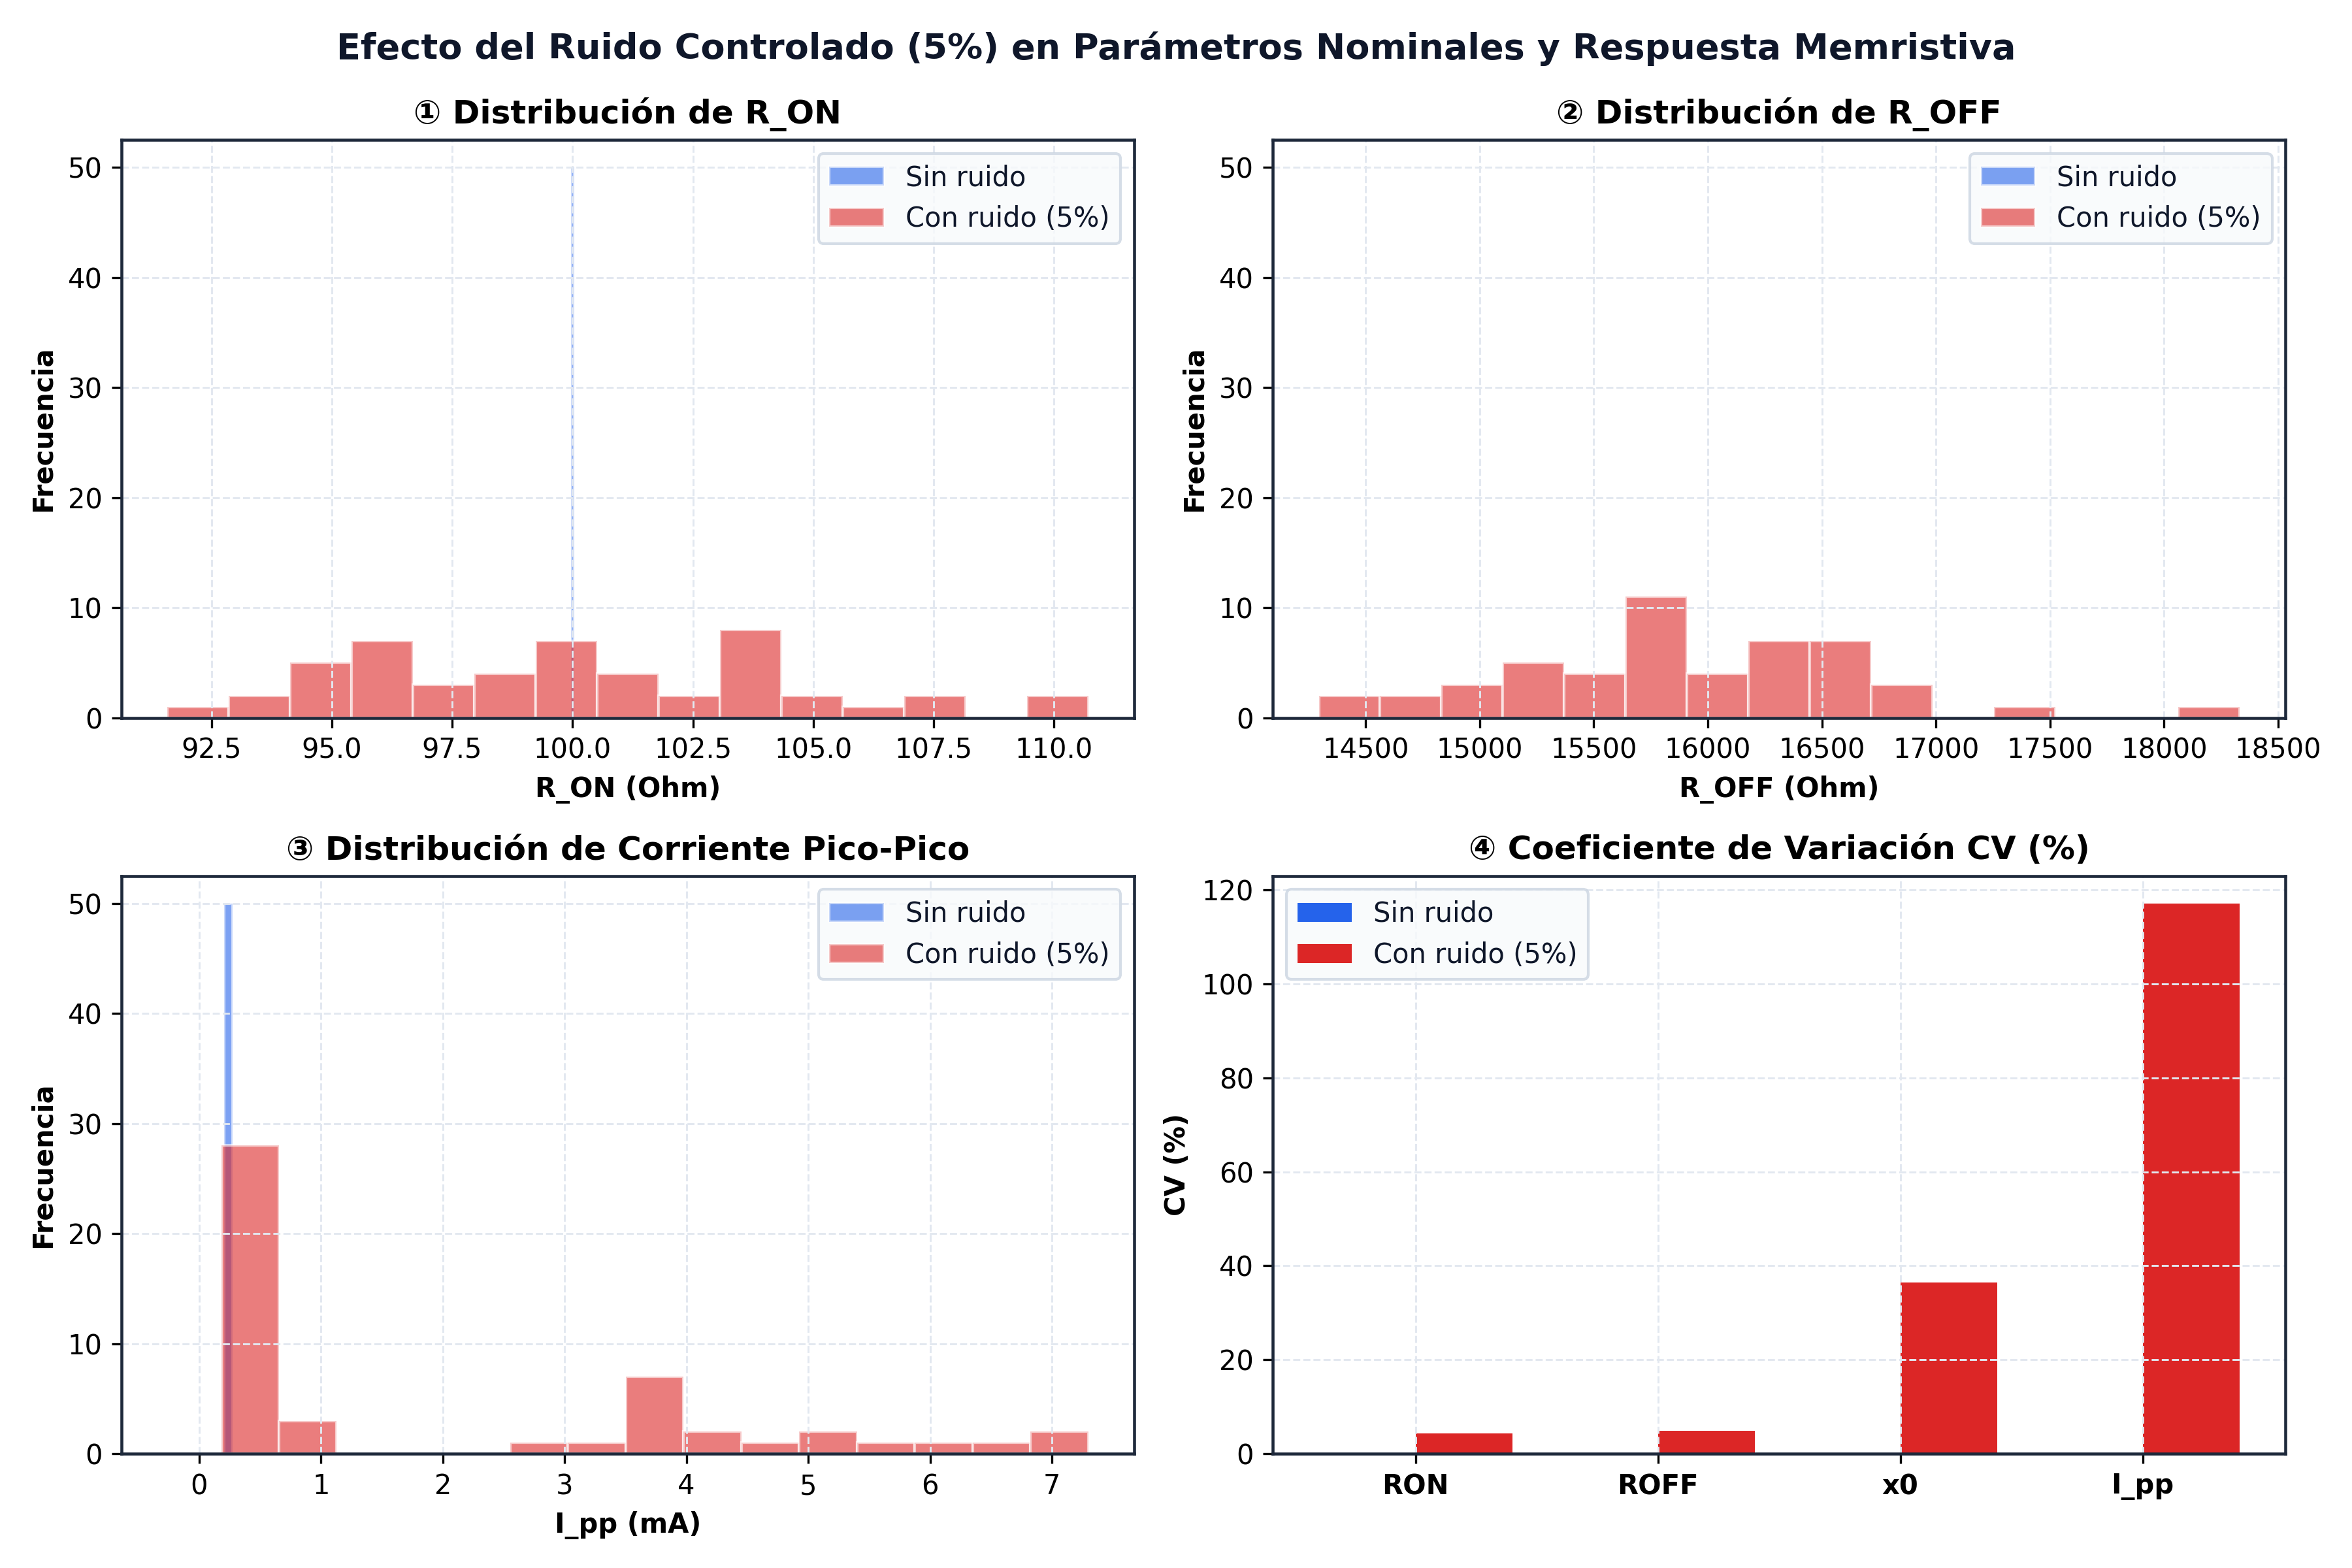
\includegraphics[width=0.7\textwidth]{figuras/fig_11_ruido.png}
    \caption{Sensibilidad del dispositivo a perturbaciones gaussianas del $5\%$ en sus parámetros nominales.}
    \label{fig:11_ruido}
\end{figure}

\textbf{Propósito y Relevancia:} La figura compara las distribuciones de $R_{\mathrm{ON}}$, $R_{\mathrm{OFF}}$ y corriente pico a pico, además del coeficiente de variación, entre dispositivos nominales y dispositivos con perturbaciones paramétricas. No representa una respuesta frecuencial ni permite concluir que el estado del memristor actúe como filtro pasa-bajos.

\begin{figure}[H]
    \centering
    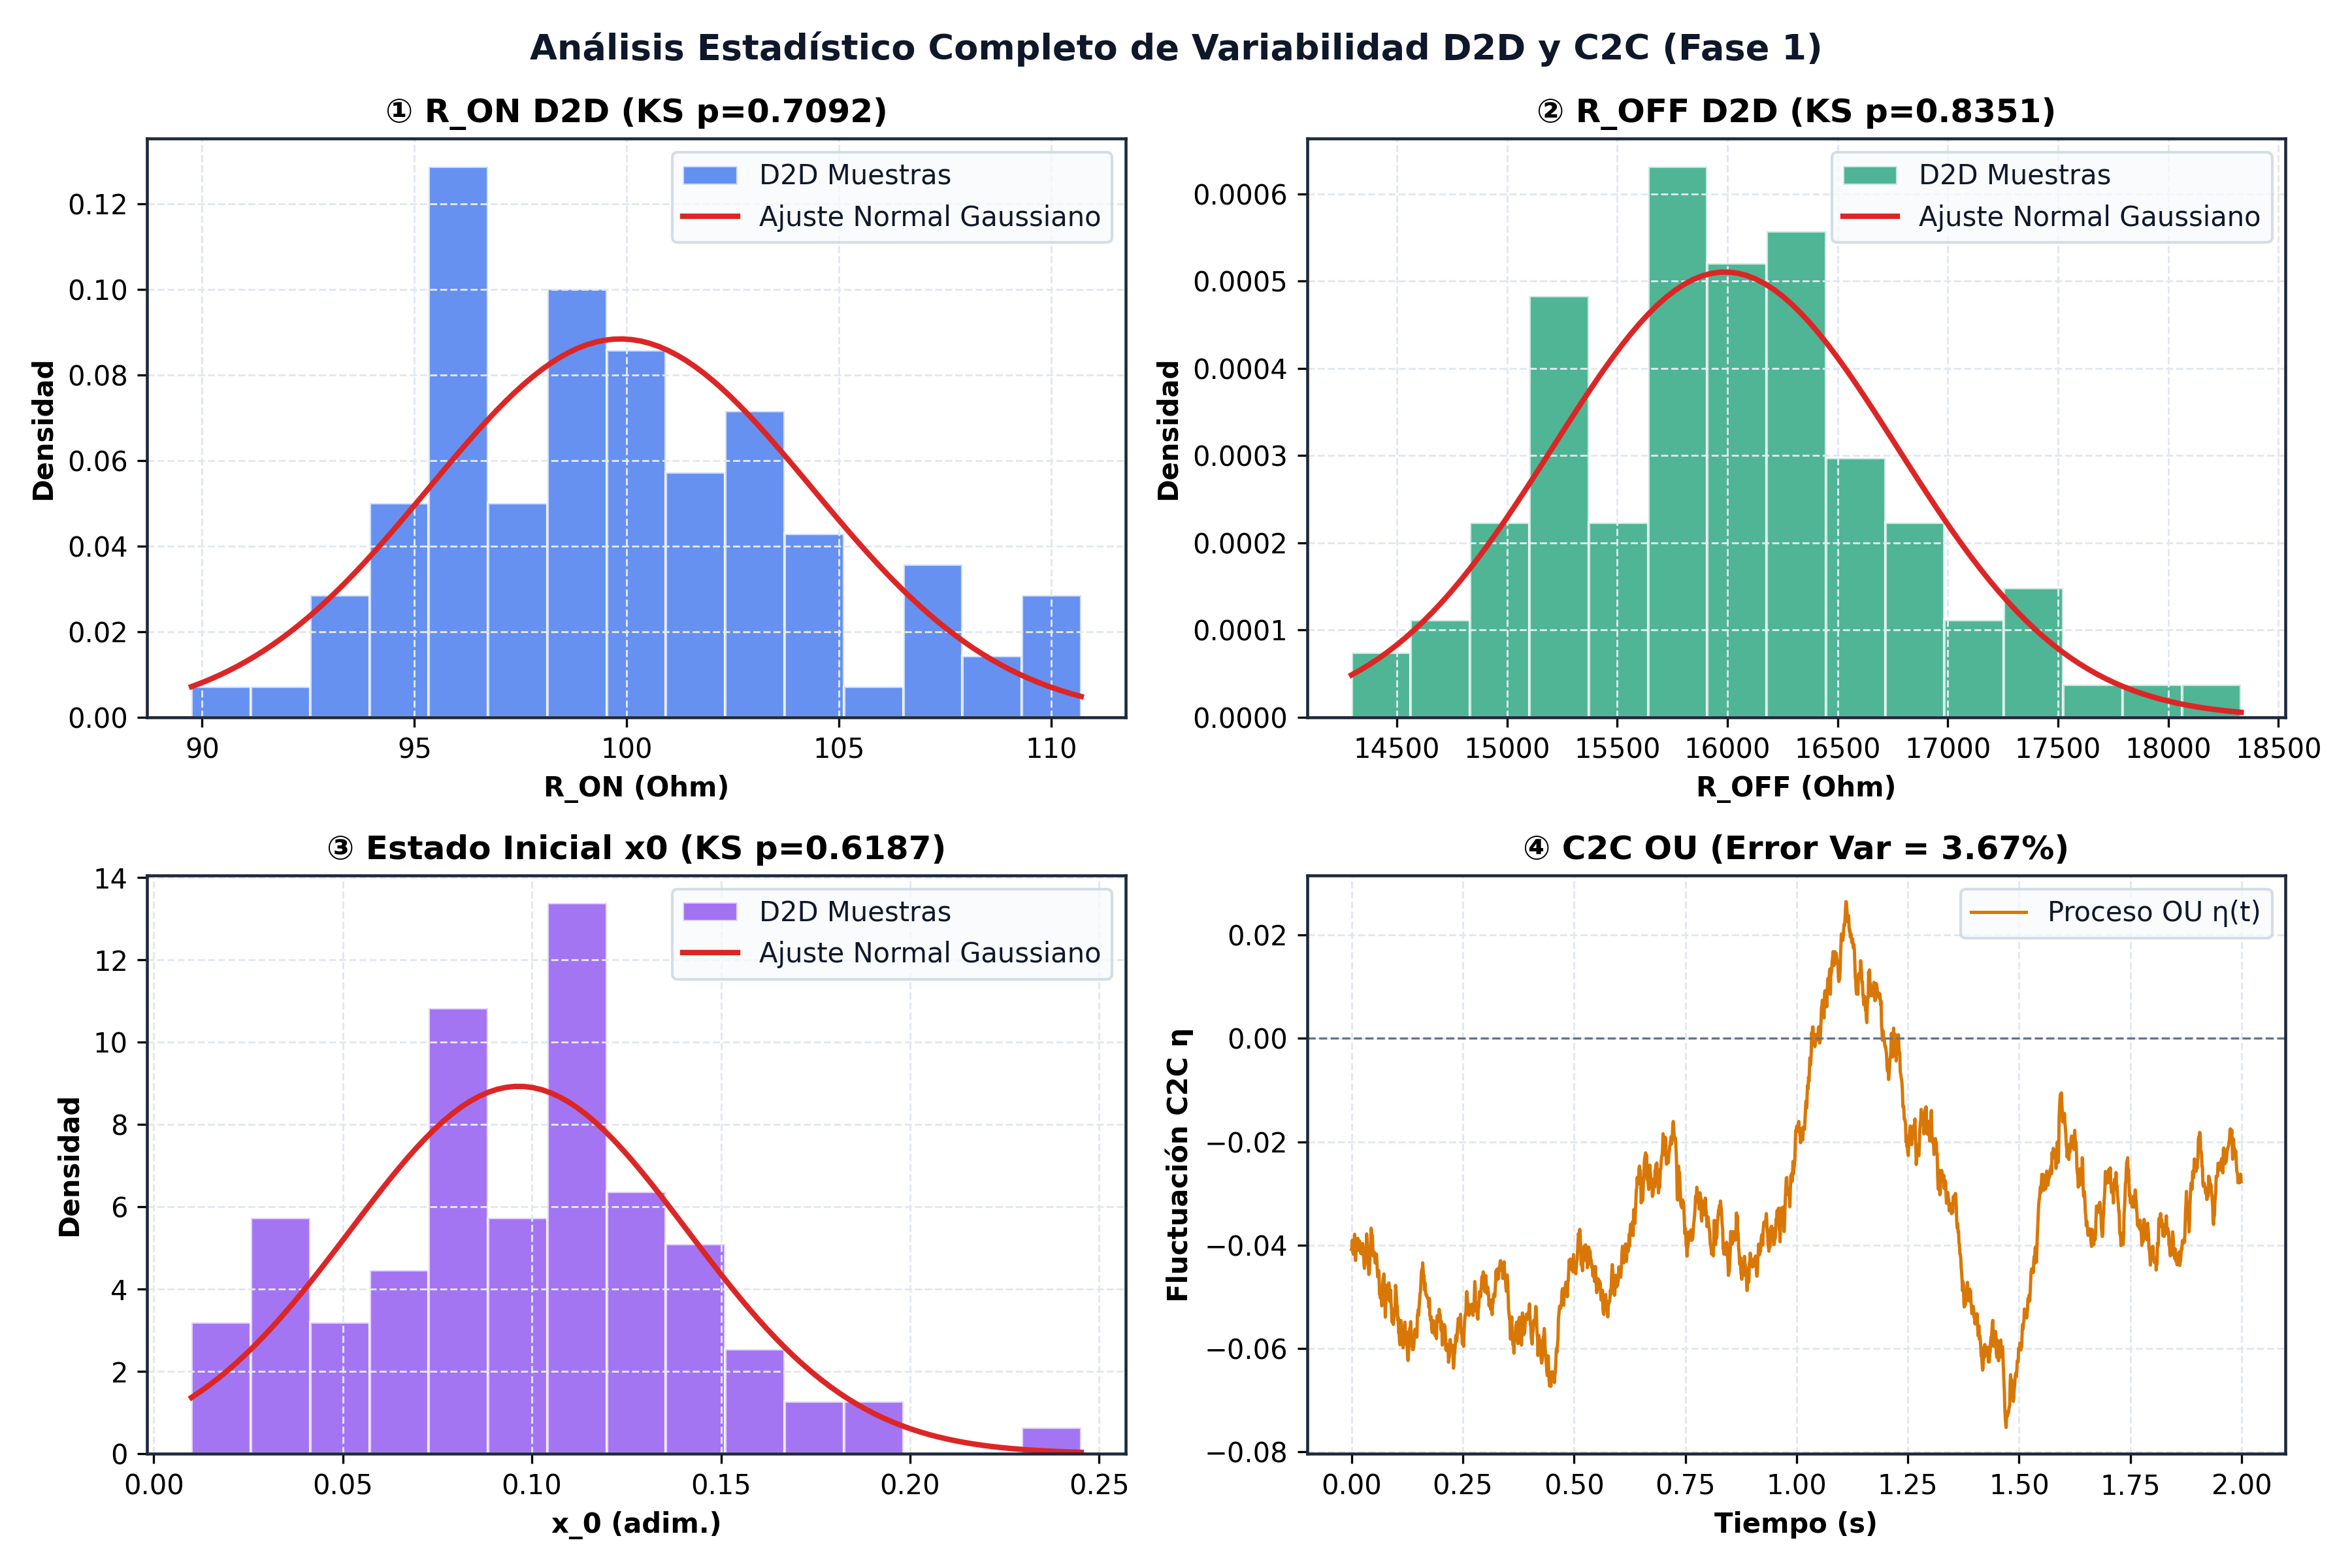
\includegraphics[width=0.8\textwidth]{figuras/fig_12_estadistica.png}
    \caption[Estadística D2D reportada]{Distribuciones D2D y pruebas KS de una corrida archivada distinta del cálculo reproducido con \texttt{05\_d2d\_c2c.py}.}
    \label{fig:12_estadistica}
\end{figure}

Los valores $p$ del panel, incluido $0.7092$ para $R_{\mathrm{ON}}$, proceden de la corrida archivada en \texttt{validacion\_estadistica\_completa.csv}, generada por \texttt{12\_estadistica.py}. Esa rutina usa una muestra distinta y ajusta media y desviación muestrales; no se revalidó la calibración del KS tras estimar esos parámetros con la misma muestra. El valor $0.8959$ informado arriba proviene de \texttt{05\_d2d\_c2c.py}, con los valores nominales para normalizar y contrastar contra $\mathcal{N}(0,1)$. Son análisis diferentes, por lo que sus $p$-valores no son intercambiables; el análisis archivado no se reprodujo en esta revisión.

\textbf{Propósito y Relevancia:} El panel reúne resúmenes estadísticos de muestras simuladas. Estos histogramas describen la población generada por el modelo; no demuestran que esa población reproduzca una distribución experimental ni validan arreglos físicos.

% =====================================================================
% Marco Práctico --- Sección 3.7: Fase 2
% =====================================================================

\subsection{Etapa 2 --- Neuronas Spiking y Sistema Híbrido}
\label{ch:fase2}

En esta segunda fase, el proyecto integra matemáticamente el modelo de neurona biológica Leaky Integrate-and-Fire (LIF) junto con el dispositivo memristivo, creando el primer bloque de construcción analógico (Memristor--Neurona) capaz de emular codificación temporal y procesamiento neuromórfico sensorial.

% =====================================================================
\subsubsection{Etapa 2.1: Neurona LIF y Acoplamiento Híbrido}
\label{sec:etapa2_1}

\paragraph{Implementación Cualitativa y Teoría Física}
El circuito híbrido simulado conecta un modelo de memristor en serie entre un estímulo de entrada (voltaje sensorial o pre-sináptico) y una neurona LIF. El potencial de membrana se representa como el voltaje de un capacitor $V_C(t)$ sujeto a una corriente de fuga paralela $R_{\mathrm{leak}}$; no se trata de un circuito físico medido.

La ecuación diferencial estocástica que rige el potencial de membrana está dada por:
\begin{equation}
C_m \frac{dV_C}{dt} = -\frac{V_C(t) - V_{\mathrm{rest}}}{R_{\mathrm{leak}}} + I_{\mathrm{inj}}(t) + \sigma_n \cdot \eta(t)
\label{eq:lif_hibrida}
\end{equation}

El acoplamiento se logra inyectando la corriente transmembrana $I_{\mathrm{inj}}(t)$, cuyo valor es dictaminado por la ley de Ohm en la rama de entrada a través de la conductancia del memristor dependiente del estado:
\begin{equation}
I_{\mathrm{inj}}(t) = \frac{V_{\mathrm{in}}(t) - V_C(t)}{R_S(x(t))}
\label{eq:i_inyectada}
\end{equation}

Cuando $V_C(t) \geq V_{\mathrm{th}}$, la neurona genera matemáticamente un evento discreto (\textit{spike}), y resetea instantáneamente su potencial a $V_{\mathrm{reset}}$, entrando en un período refractario absoluto.

Para representar un \textit{sensor volátil}, se emplea un modelo computacional inspirado en dióxido de hafnio (HfO$_2$). Incluye un término fenomenológico de relajación del estado en ausencia de estímulo:
\begin{equation}
\frac{dx}{dt} = f(V_M, x) - \frac{x}{\tau_{\mathrm{relax}}} \left(1 - H(V_M - V_{\mathrm{hold}})\right)
\label{eq:hfo2_dinamica}
\end{equation}

Cualitativamente (Figura~\ref{fig:hfo2_isi_hibrido}), en la simulación el estímulo de $1.5\,\mathrm{V}$ cambia el estado y la resistencia del modelo memristivo, modificando la corriente de entrada y los intervalos entre disparos. La figura ilustra adaptación temporal dentro de este modelo; no demuestra transducción biológica ni una respuesta de un dispositivo fabricado.

\begin{figure}[H]
    \centering
    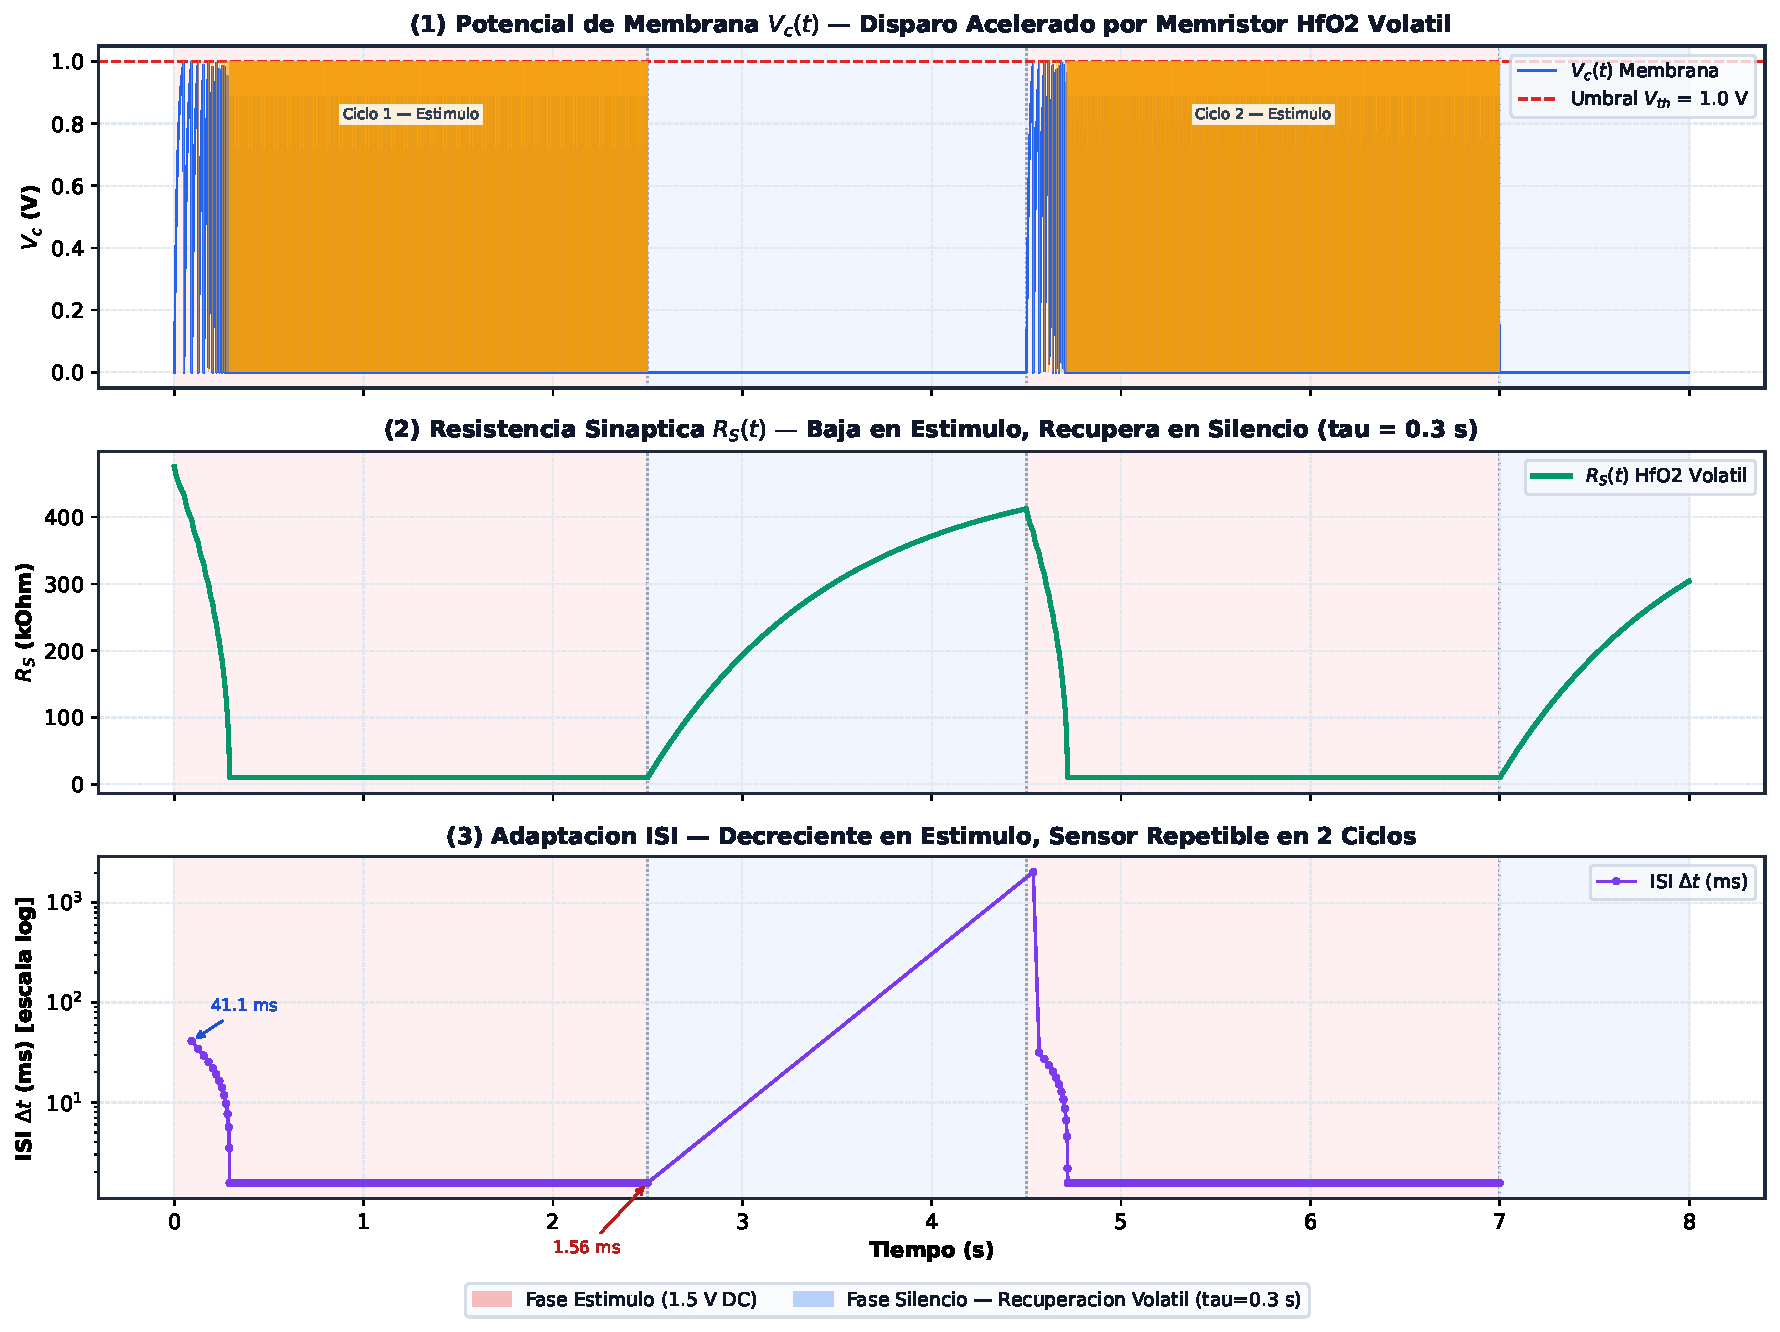
\includegraphics[width=0.85\textwidth]{figuras/fig_06_hfo2_isi_legible.pdf}
    \caption{Respuesta cualitativa del sistema híbrido: Potencial de membrana $V_C(t)$ evidenciando la aceleración temporal (top), Resistencia $R_S(t)$ descendente (centro), e Intervalo Inter-Spike (ISI) modularizado (abajo).}
    \label{fig:hfo2_isi_hibrido}
\end{figure}

\textbf{Propósito y Relevancia:} La figura ilustra el acoplamiento implementado entre el modelo memristivo y la neurona LIF. No constituye una validación de un sensor físico ni de un receptor nociceptivo.

\paragraph{Validación Cuantitativa Computacional}
La integridad matemática de esta fase fue comprobada contra soluciones exactas y papers de referencia del estado del arte.

\begin{figure}[H]
    \centering
    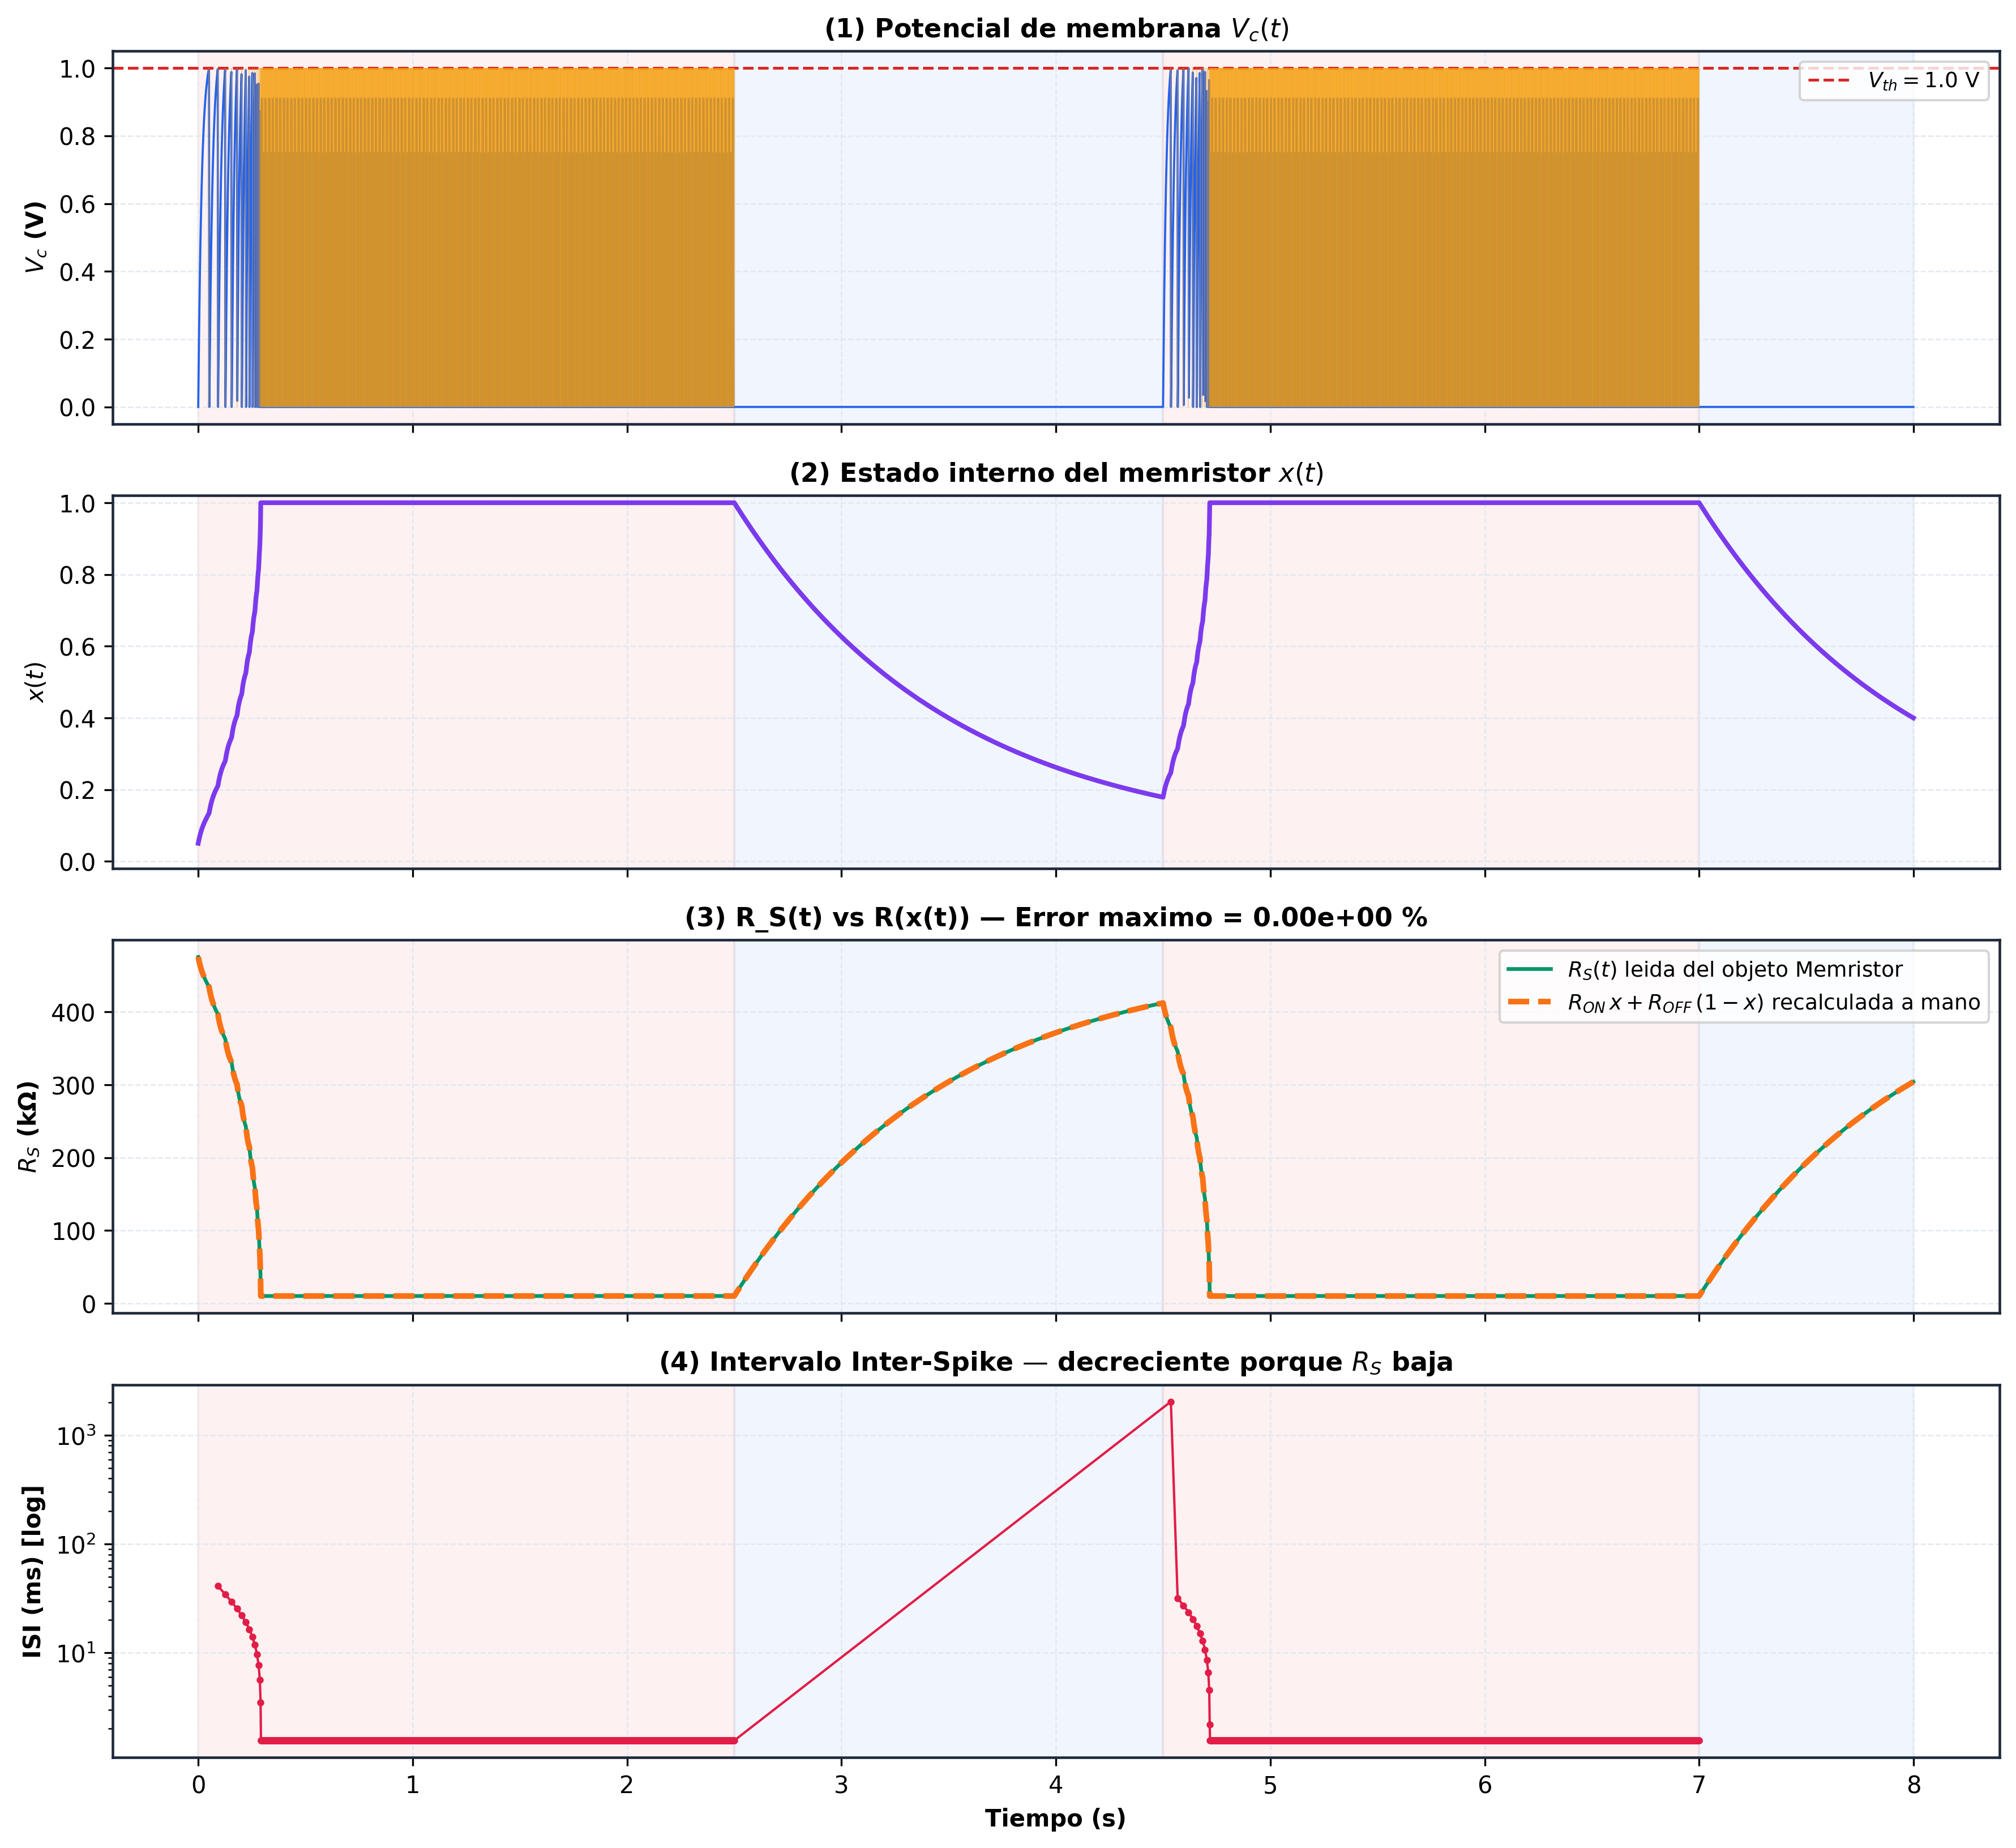
\includegraphics[width=0.7\textwidth]{figuras/fig_08_rs_x.png}
    \caption{Verificación de la resistencia en serie $R_S$ proveniente de la dinámica de acoplamiento de $x$.}
    \label{fig:08_rs_x}
\end{figure}

\textbf{Propósito y Relevancia:} Este gráfico comprueba, para la ejecución y las variables mostradas, la consistencia entre $R_S$ y $x(t)$ según la relación implementada. No prueba por sí solo ausencia general de pérdida de eventos, retrasos ni errores en todas las ejecuciones.

\textbf{Solución Analítica LIF Subumbral:}
Se sometió el módulo integrador numérico de la neurona LIF a una validación estricta frente a su solución analítica exacta de circuito RC subumbral:
\begin{equation}
V_m(t) = V_{\infty} + (V_{m,0} - V_{\infty}) e^{-t/\tau_{eq}}
\end{equation}
La comparación cuantitativa entre la simulación discreta y la solución RC analítica es distinta de la comparación cualitativa con Wang descrita más adelante. En el CSV archivado \texttt{lif\_rc\_validation.csv}, el cálculo de $R^2$ sobre las 1000 muestras disponibles es $0.9999815$, que redondeado a cuatro decimales da $1.0000$. Este resultado describe solo esa prueba subumbral y no se atribuye a la comparación cualitativa ni demuestra exactitud general del integrador para otros pasos o condiciones.

\begin{figure}[H]
    \centering
    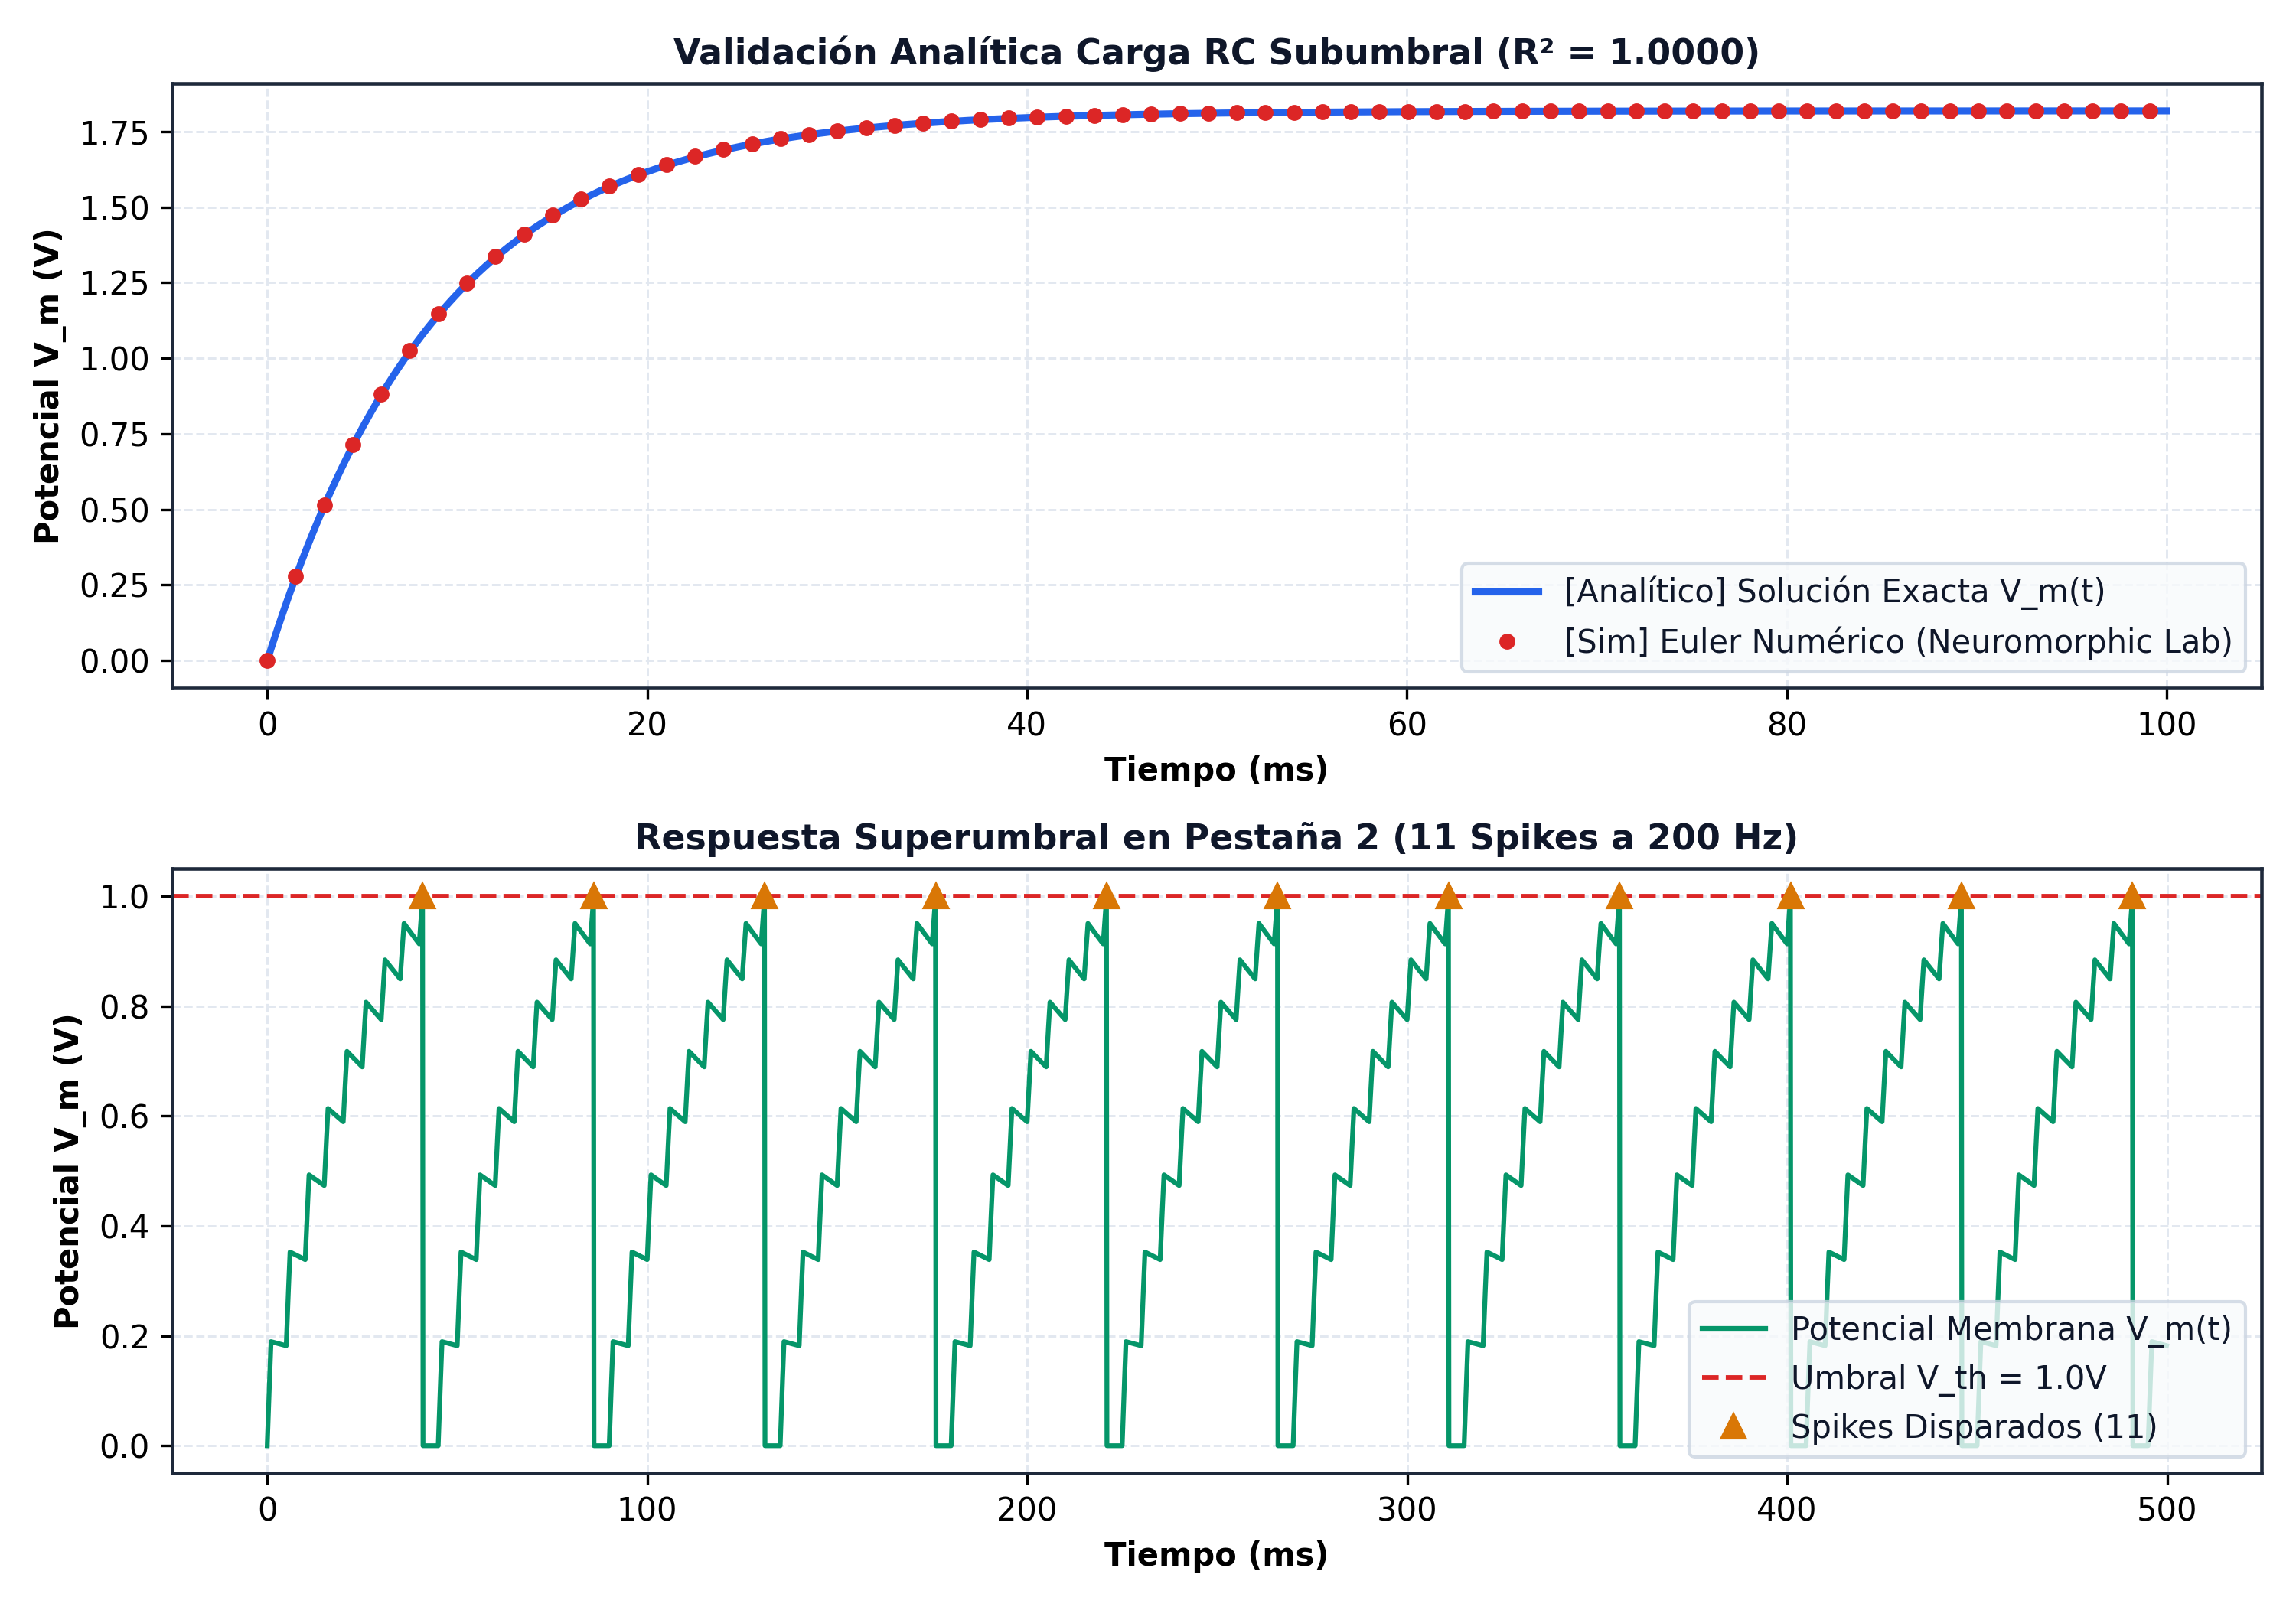
\includegraphics[width=0.85\textwidth]{figuras/fig_03_lif.png}
    \caption{Validación analítica subumbral de la neurona LIF frente a la solución RC exacta en respuesta al impulso.}
    \label{fig:val-lif}
\end{figure}

\textbf{Propósito y Relevancia:} La comparación permite evaluar la respuesta subumbral para las condiciones ensayadas. El valor archivado no basta para descartar sesgos algorítmicos en otras configuraciones ni para afirmar que el núcleo esté libre de errores.

\textbf{Comportamiento cualitativo de integración y disparo LIF:}
La neurona LIF del simulador comparte el comportamiento funcional descrito por Wang et al.~\cite{2}: integra los estímulos, alcanza el umbral y genera eventos de disparo con reinicio. La Figura~\ref{fig:lif-behavior-wang} muestra esta secuencia en el simulador \texttt{Neuromorphic Lab}, con la configuración guardada en \url{02_SOFTWARE/neuromorphic_lab/configs/lif_config.json}: $C_m=100\,\mathrm{nF}$, $R_S=100\,\mathrm{k\Omega}$, $R_{\mathrm{leak}}=1\,\mathrm{M\Omega}$, umbral de $1\,\mathrm{V}$ y período refractario de $2\,\mathrm{ms}$. La entrada simulada es un tren unipolar de $2\,\mathrm{V}$ a $200\,\mathrm{Hz}$, con ciclo útil del $20\%$, durante $0.5\,\mathrm{s}$. Con paso de integración de $1\,\mathrm{\mu s}$, esta ejecución produce 11 eventos de disparo.

\begin{figure}[H]
    \centering
    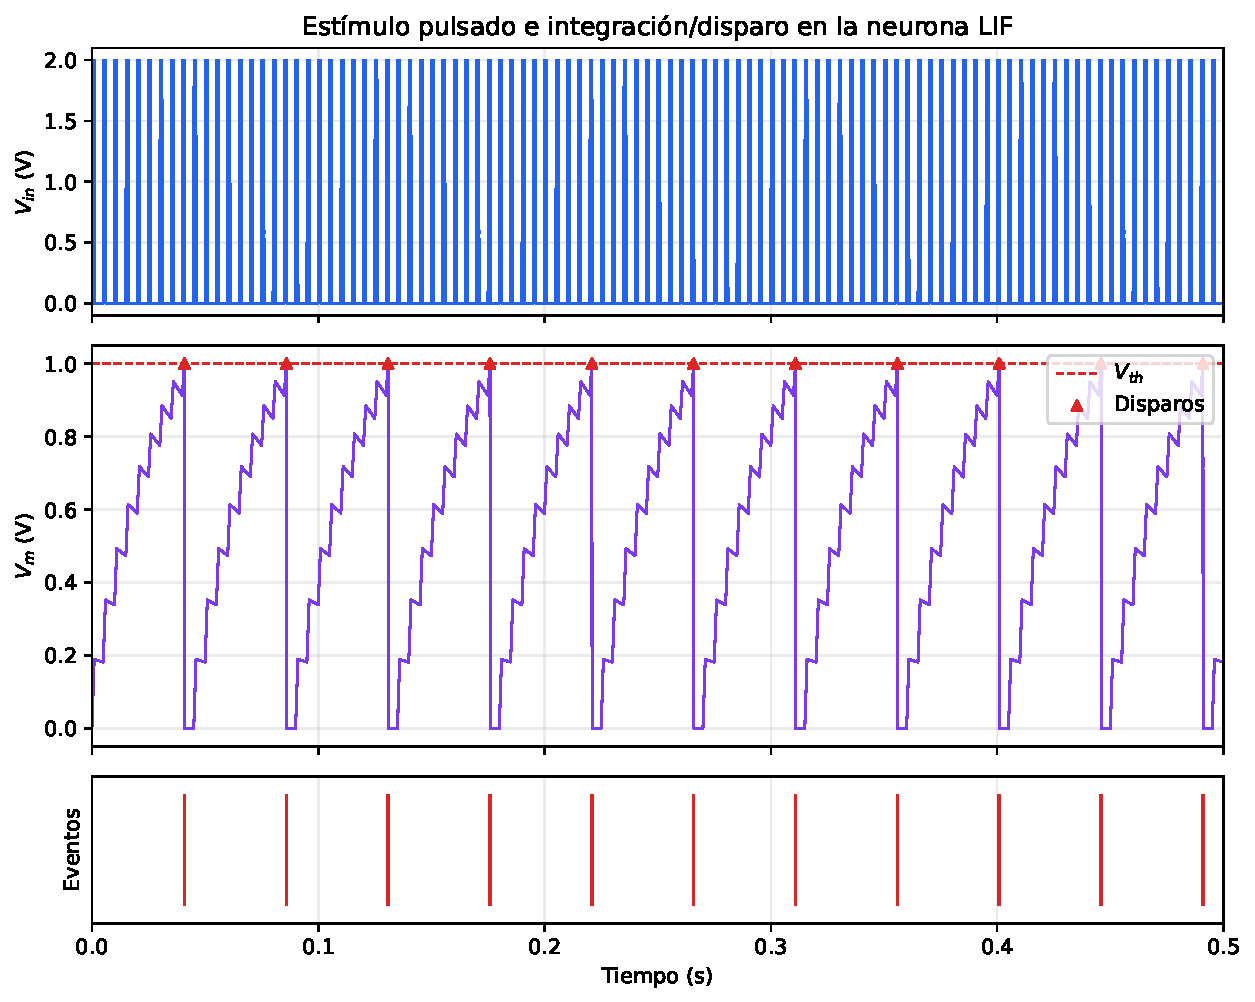
\includegraphics[width=0.95\textwidth]{figuras/fig_13_lif_behavior.pdf}
    \caption[Respuesta de la neurona LIF]{Respuesta de la neurona LIF del simulador: estímulo pulsado, integración del potencial de membrana y eventos de disparo, en concordancia funcional con la dinámica descrita por Wang et al.~\cite{2}.}
    \label{fig:lif-behavior-wang}
\end{figure}

\textbf{Propósito y Relevancia:} La figura documenta que el simulador LIF implementa la secuencia de integración y disparo. El panel inferior es un raster de eventos, no una forma de onda de voltaje de salida ni una medición física.

% =====================================================================
% Marco Práctico --- Sección 3.8: Fase 3
% =====================================================================

\subsection{Etapa 3 --- Plasticidad Sináptica}
\label{ch:fase3}

Esta fase describe simulaciones de plasticidad LTP/LTD y STDP con modelos
memristivos. Las comparaciones con Jo et al. (2010) se recalcularon con
el protocolo y las particiones descritos abajo, usando puntos
digitalizados de las figuras publicadas. No son mediciones propias ni
certifican por sí solas una respuesta física.

% =====================================================================
\subsubsection{Etapa 3.1: LTP/LTD y STDP}
\label{sec:etapa3_1}

\paragraph{Implementación Cualitativa (LTP/LTD)}
Para estudiar la respuesta acumulativa de la conductancia sináptica (representando el peso lógico $W_{ij}$), se aplicaron secuencias controladas de trenes de pulsos de voltaje idénticos. Matemáticamente, cada pulso induce un minúsculo diferencial $dx$ positivo o negativo sobre el estado del filamento según su polaridad. 

Los pulsos positivos inducen la Potenciación a Largo Plazo (LTP), aumentando la conductancia de forma progresiva. Los pulsos negativos provocan la Depresión a Largo Plazo (LTD), borrando la historia almacenada. La Figura~\ref{fig:20_vi_ltp_ltd} documenta voltaje, corriente, resistencia y conductancia durante pulsos LTP/LTD; la curva temporal escalonada descrita en el informe previo no tiene una figura independiente incluida en este paquete.

El ajuste STDP y sus puntos reservados se muestran en la Figura~\ref{fig:stdp_curve_ch3} del Cap\'itulo~3. Se conserva aqu\'i la interpretaci\'on ampliada de la partici\'on y sus l\'imites.

\textbf{Propósito y Relevancia:} La figura documenta la asimetría del conjunto digitalizado y el error de predicción en los puntos reservados. No certifica la precisión de un cambio de conductancia físico ni la validez general del componente.

\textbf{Curva LTP/LTD atribuida a Jo et al.}
El CSV \texttt{jo2010\_ltp\_ltd.csv} contiene 87 puntos atribuidos por el
validador a la Fig.~2a; no son 200 registros experimentales brutos. Se
simularon 100 pulsos SET de $+3.2\,\mathrm{V}$ y 100 RESET de
$-2.8\,\mathrm{V}$, ambos de $300\,\mu\mathrm{s}$, con lecturas a
$1\,\mathrm{V}$. De los 87 puntos, dos quedan fuera del intervalo de
0--200 pulsos; los 85 restantes se separan, dentro de cada rama, en
bloques contiguos 60/20/20: 50 de entrenamiento, 17 de validación y 18
de test. Se ajustan $R_{\mathrm{on}}$, $R_{\mathrm{off}}$, el coeficiente
de deriva efectivo y $x_0$ solo con entrenamiento; validación selecciona
entre tres inicializaciones. No se aplica un reescalado min--max ni una
calibración afín posterior. En test se obtuvo
$R^2_{\mathrm{residual}}=0.73988$, MAE $=8.3491\,\mathrm{nA}$,
RMSE $=8.6181\,\mathrm{nA}$ y ERP $=31.23\%$. Por rama, el resultado es
deficiente: $R^2=-8.54$ en LTP ($n=10$) y $R^2=-829.99$ en LTD ($n=8$).
Pearson agregado es $r=0.99303$ ($r^2=0.98610$), pero este valor mide
covariación y no sustituye el $R^2_{\mathrm{residual}}$: la predicción
de LTP es constante, por lo que su correlación no está definida; en LTD
se obtiene $r=-0.22170$ ($r^2=0.04915$).
Los parámetros efectivos se ajustan a la misma curva digitalizada y no
son una caracterización independiente del dispositivo; la evidencia es
parcial y no demuestra predicción independiente ni validación completa
del artículo.

La comparaci\'on LTP/LTD y sus puntos reservados se muestran en la Figura~\ref{fig:ltp_ltd_curve_ch3} del Cap\'itulo~3; se conserva aqu\'i el an\'alisis cuantitativo por rama.

\textbf{Propósito y Relevancia:} La figura muestra la forma de la curva bajo la normalización declarada. No demuestra fidelidad física general ni identifica un mecanismo microscópico concreto.


\begin{figure}[H]
    \centering
    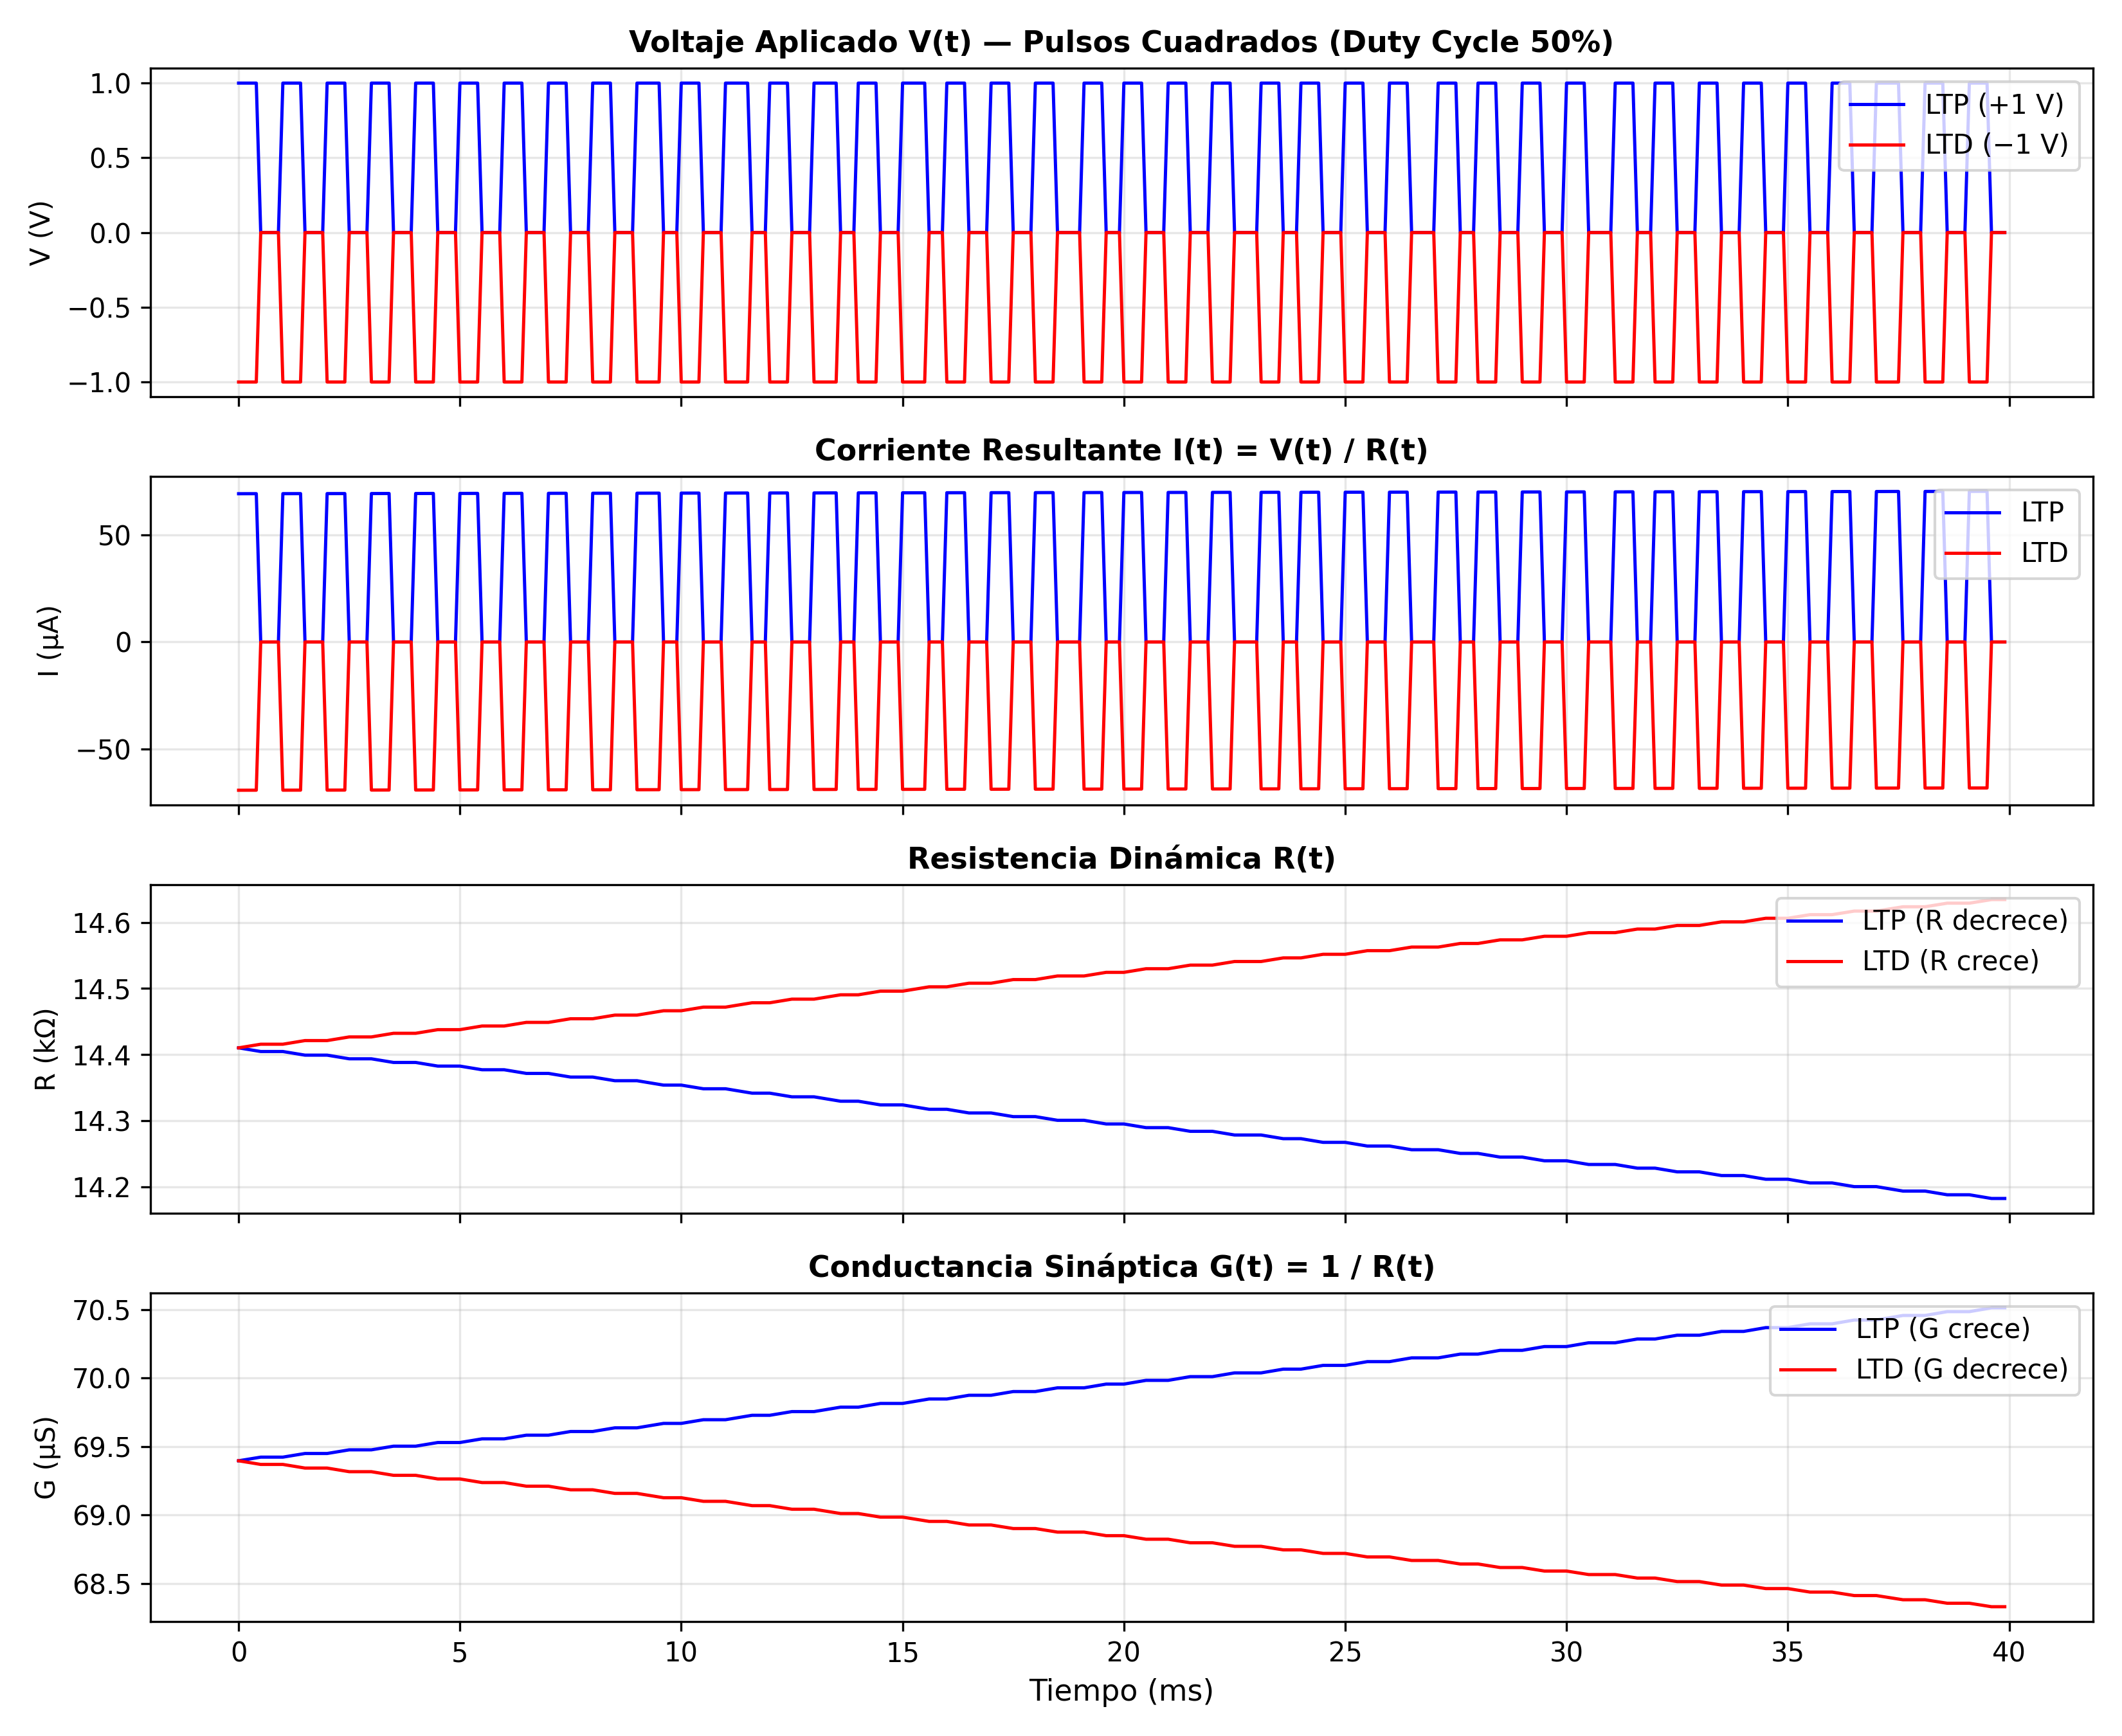
\includegraphics[width=0.7\textwidth]{figuras/fig_20_vi_ltp_ltd.png}
    \caption{Caracterización simultánea de voltaje, corriente, resistencia y conductancia durante pulsos LTP y LTD.}
    \label{fig:20_vi_ltp_ltd}
\end{figure}

\textbf{Propósito y Relevancia:} La figura muestra variables registradas por la simulación durante los pulsos. No constituye una observación microscópica ni una prueba general de conservación para otras configuraciones.

% =====================================================================
% Marco Práctico --- Sección 3.9: Etapa 4
% =====================================================================

\subsection{Etapa 4 --- Arquitecturas Matriciales y No Idealidades}
\label{ch:fase4}

La Etapa 4 estudia implementaciones a nivel de red mediante un
arreglo cruzado bidimensional (crossbar). Su aplicación al agente de
control se desarrolla en la subseccion siguiente. Los resultados
corresponden a modelos y entornos de simulación, no a mediciones de
un crossbar fabricado.

% =====================================================================
\subsubsection{Etapa 4.1: Matriz Crossbar e In-Memory}
\label{sec:etapa4_1}

Una matriz crossbar se representa por
$\mathbf{G}\in\mathbb{R}^{N\times M}$, con $N$ filas de entrada y
$M$ columnas de salida; cada intersección aloja un dispositivo
memristivo simulado.

En el modelo ideal, al aplicar un vector de voltajes de entrada
$\mathbf{V}=[V_1,V_2,\dots,V_N]^{\mathsf T}\in\mathbb{R}^{N}$ a las
filas, las conductancias en paralelo realizan una multiplicación
matriz-vector. La corriente $I_j$ de cada columna sigue la ley de Ohm
y la ley de corrientes de Kirchhoff:

\begin{equation}
I_j(t) = \sum_{i=1}^N V_i(t) \cdot G_{ij}(t) \quad \implies \quad \mathbf{I} = \mathbf{G}^{\mathsf T} \mathbf{V},\qquad \mathbf{I}\in\mathbb{R}^{M}
\label{eq:vmm_law}
\end{equation}

En un arreglo analógico ideal, las contribuciones de las celdas se procesarían en paralelo. Esta descripción algebraica no demuestra latencia física constante ni complejidad computacional $\mathcal{O}(1)$ para el solver numérico: el costo de resolver el modelo MNA se trata por separado en el Experimento~9.

\paragraph{Implementación Cualitativa (Operación Analógica $1 \times 1$)}
Se implementó y se visualizó estructuralmente el sistema base modular probando una celda atómica unitaria que simula la interacción macro-escalar. 

Como se ilustra en las salidas de simulación (Figuras~\ref{fig:crossbar_1x1_completo}a-d), al suministrar la onda cuadrada de voltaje al modelo, la dinámica de la celda memristiva de Yakopcic cambia su estado. La línea de columna calcula $\mathbf{I}=\mathbf{G}^{\mathsf T}\mathbf{V}$ en el modelo, con las filas de $\mathbf{G}$ asociadas a las entradas y las columnas a las salidas. Estas figuras ilustran la operación implementada; no son mediciones de hardware ni prueban por sí solas su comportamiento físico.

\begin{figure}[H]
    \centering
    \begin{subfigure}[b]{0.84\textwidth}
        \centering
        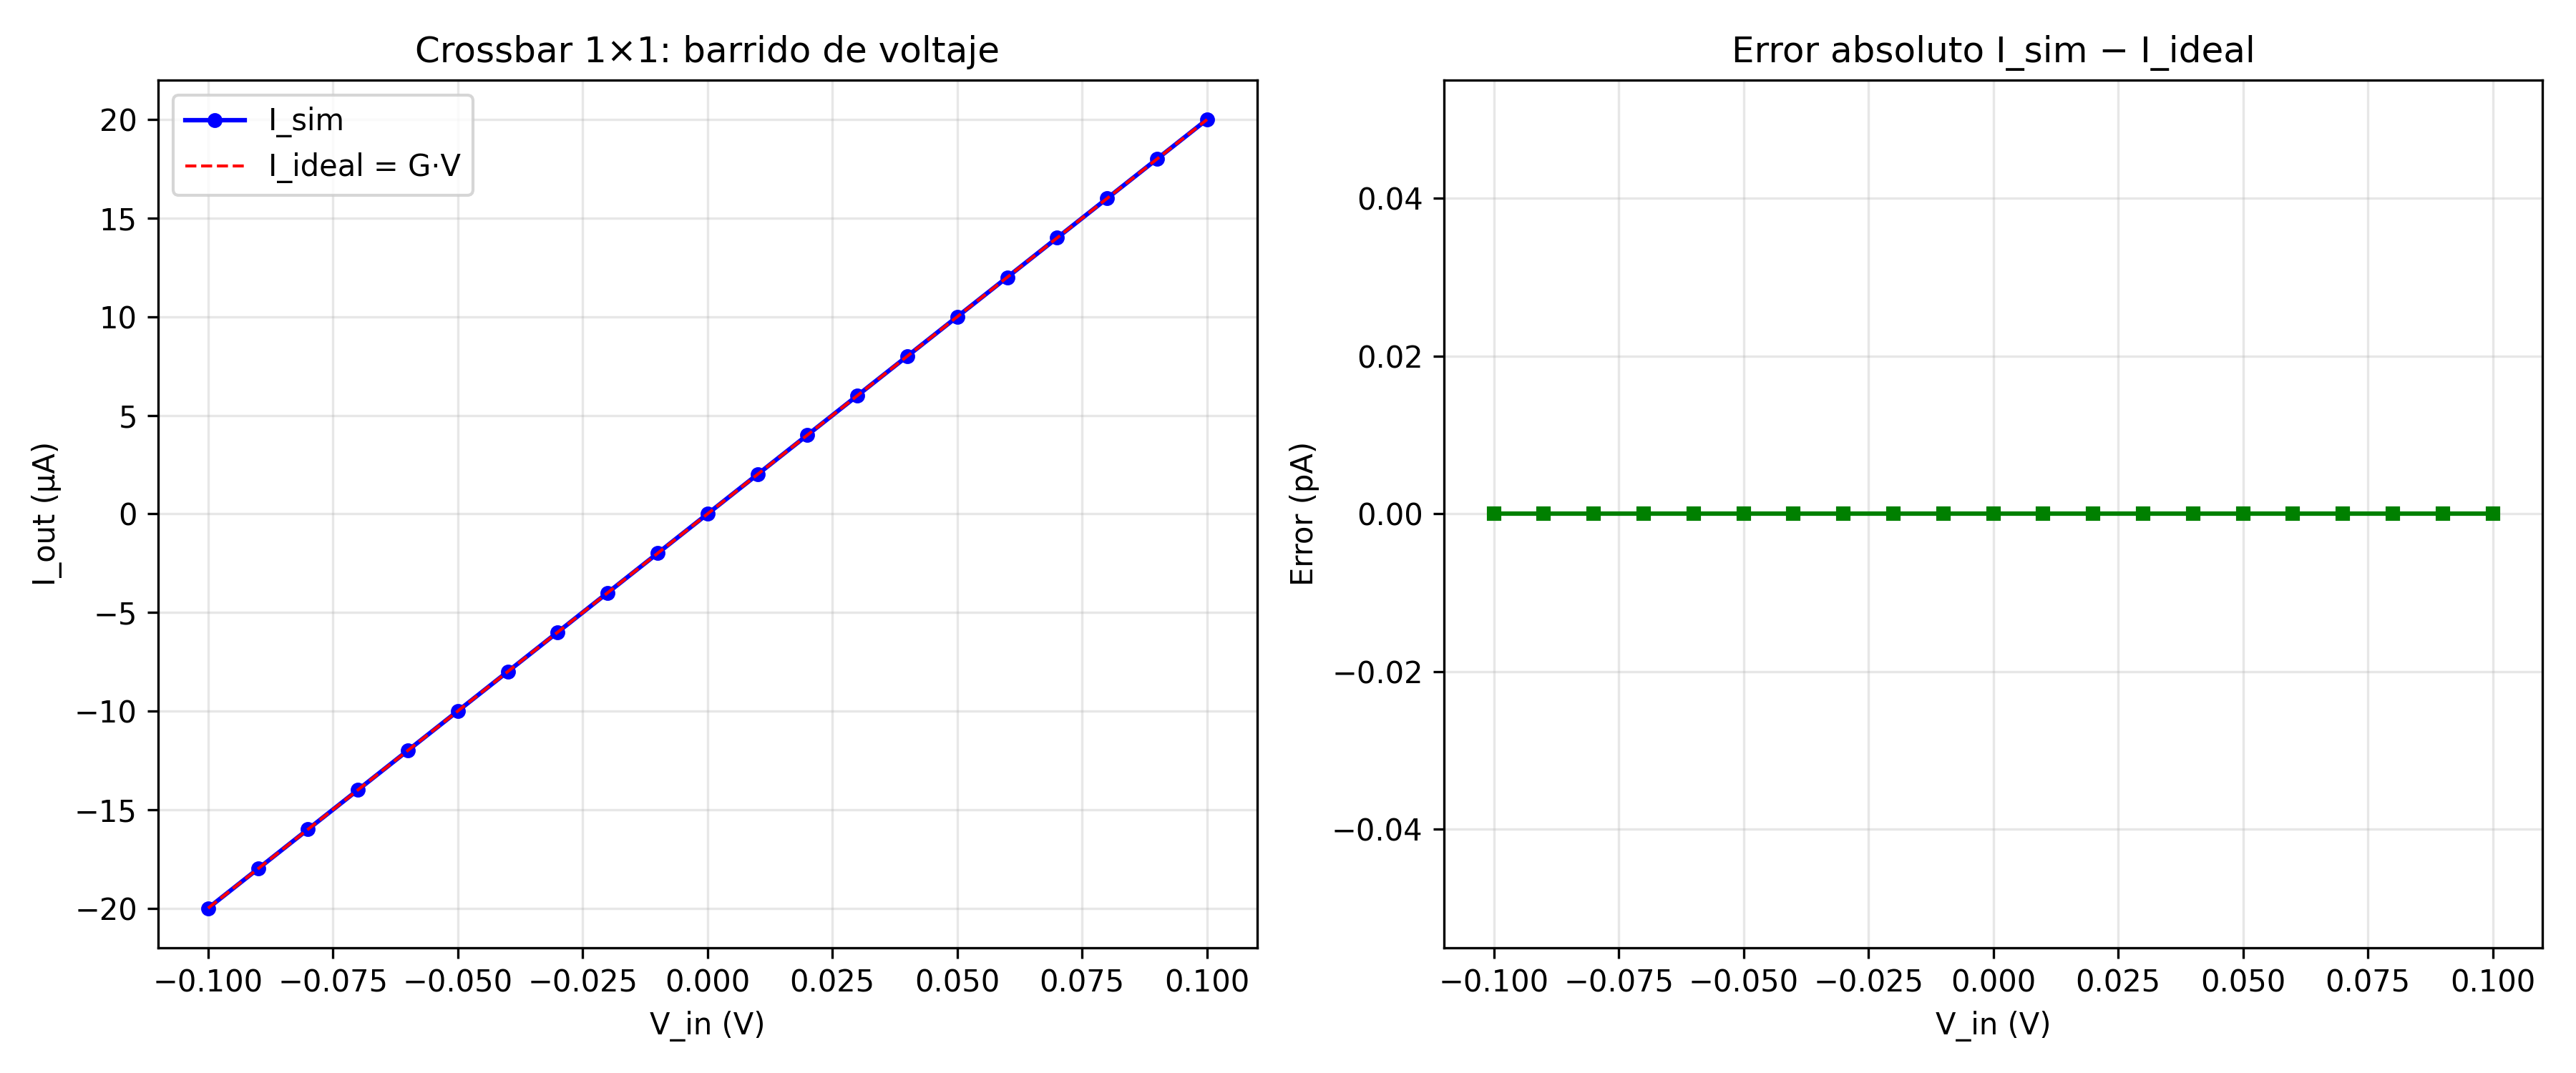
\includegraphics[width=\textwidth]{figuras/fig_21a_crossbar_V.png}
        \caption{Pulsos de excitación por línea de Palabra $V_i(t)$.}
    \end{subfigure}
    \vskip 0.3cm
    \begin{subfigure}[b]{0.84\textwidth}
        \centering
        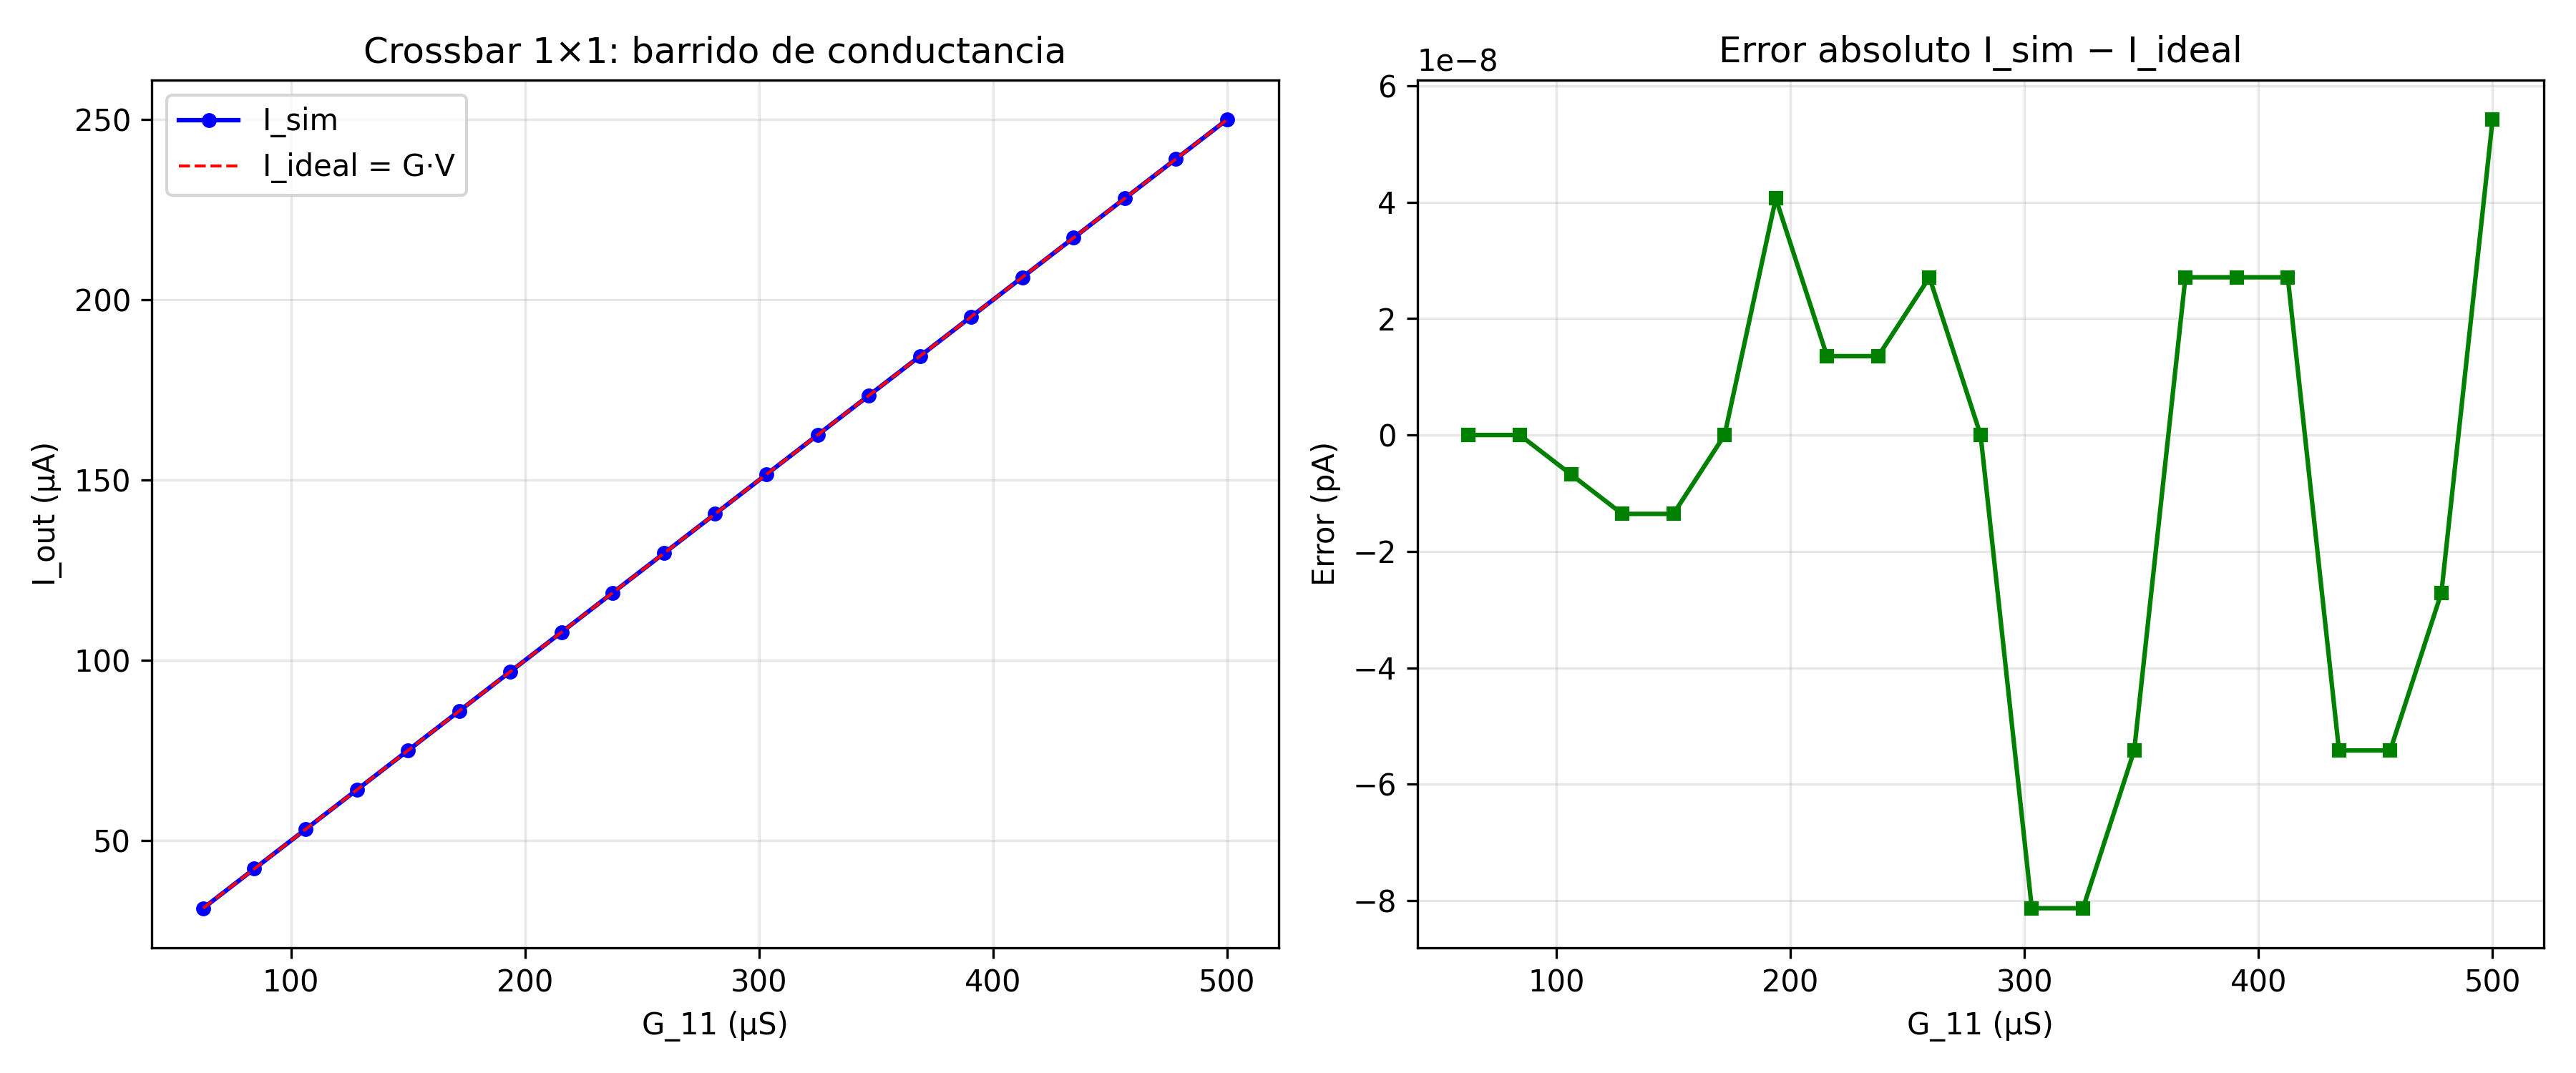
\includegraphics[width=\textwidth]{figuras/fig_21b_crossbar_G.png}
        \caption{Matriz espacial de conductancia transversal $G_{ij}(t)$.}
    \end{subfigure}
    \caption[Verificación funcional del crossbar analógico]{Verificación cualitativa y funcional de computación In-Memory en el bloque elemental Crossbar analógico (paneles a y b).}
    \label{fig:crossbar_1x1_completo}
\end{figure}

\clearpage

\begin{figure}[H]
    \ContinuedFloat
    \centering
    \begin{subfigure}[b]{0.84\textwidth}
        \centering
        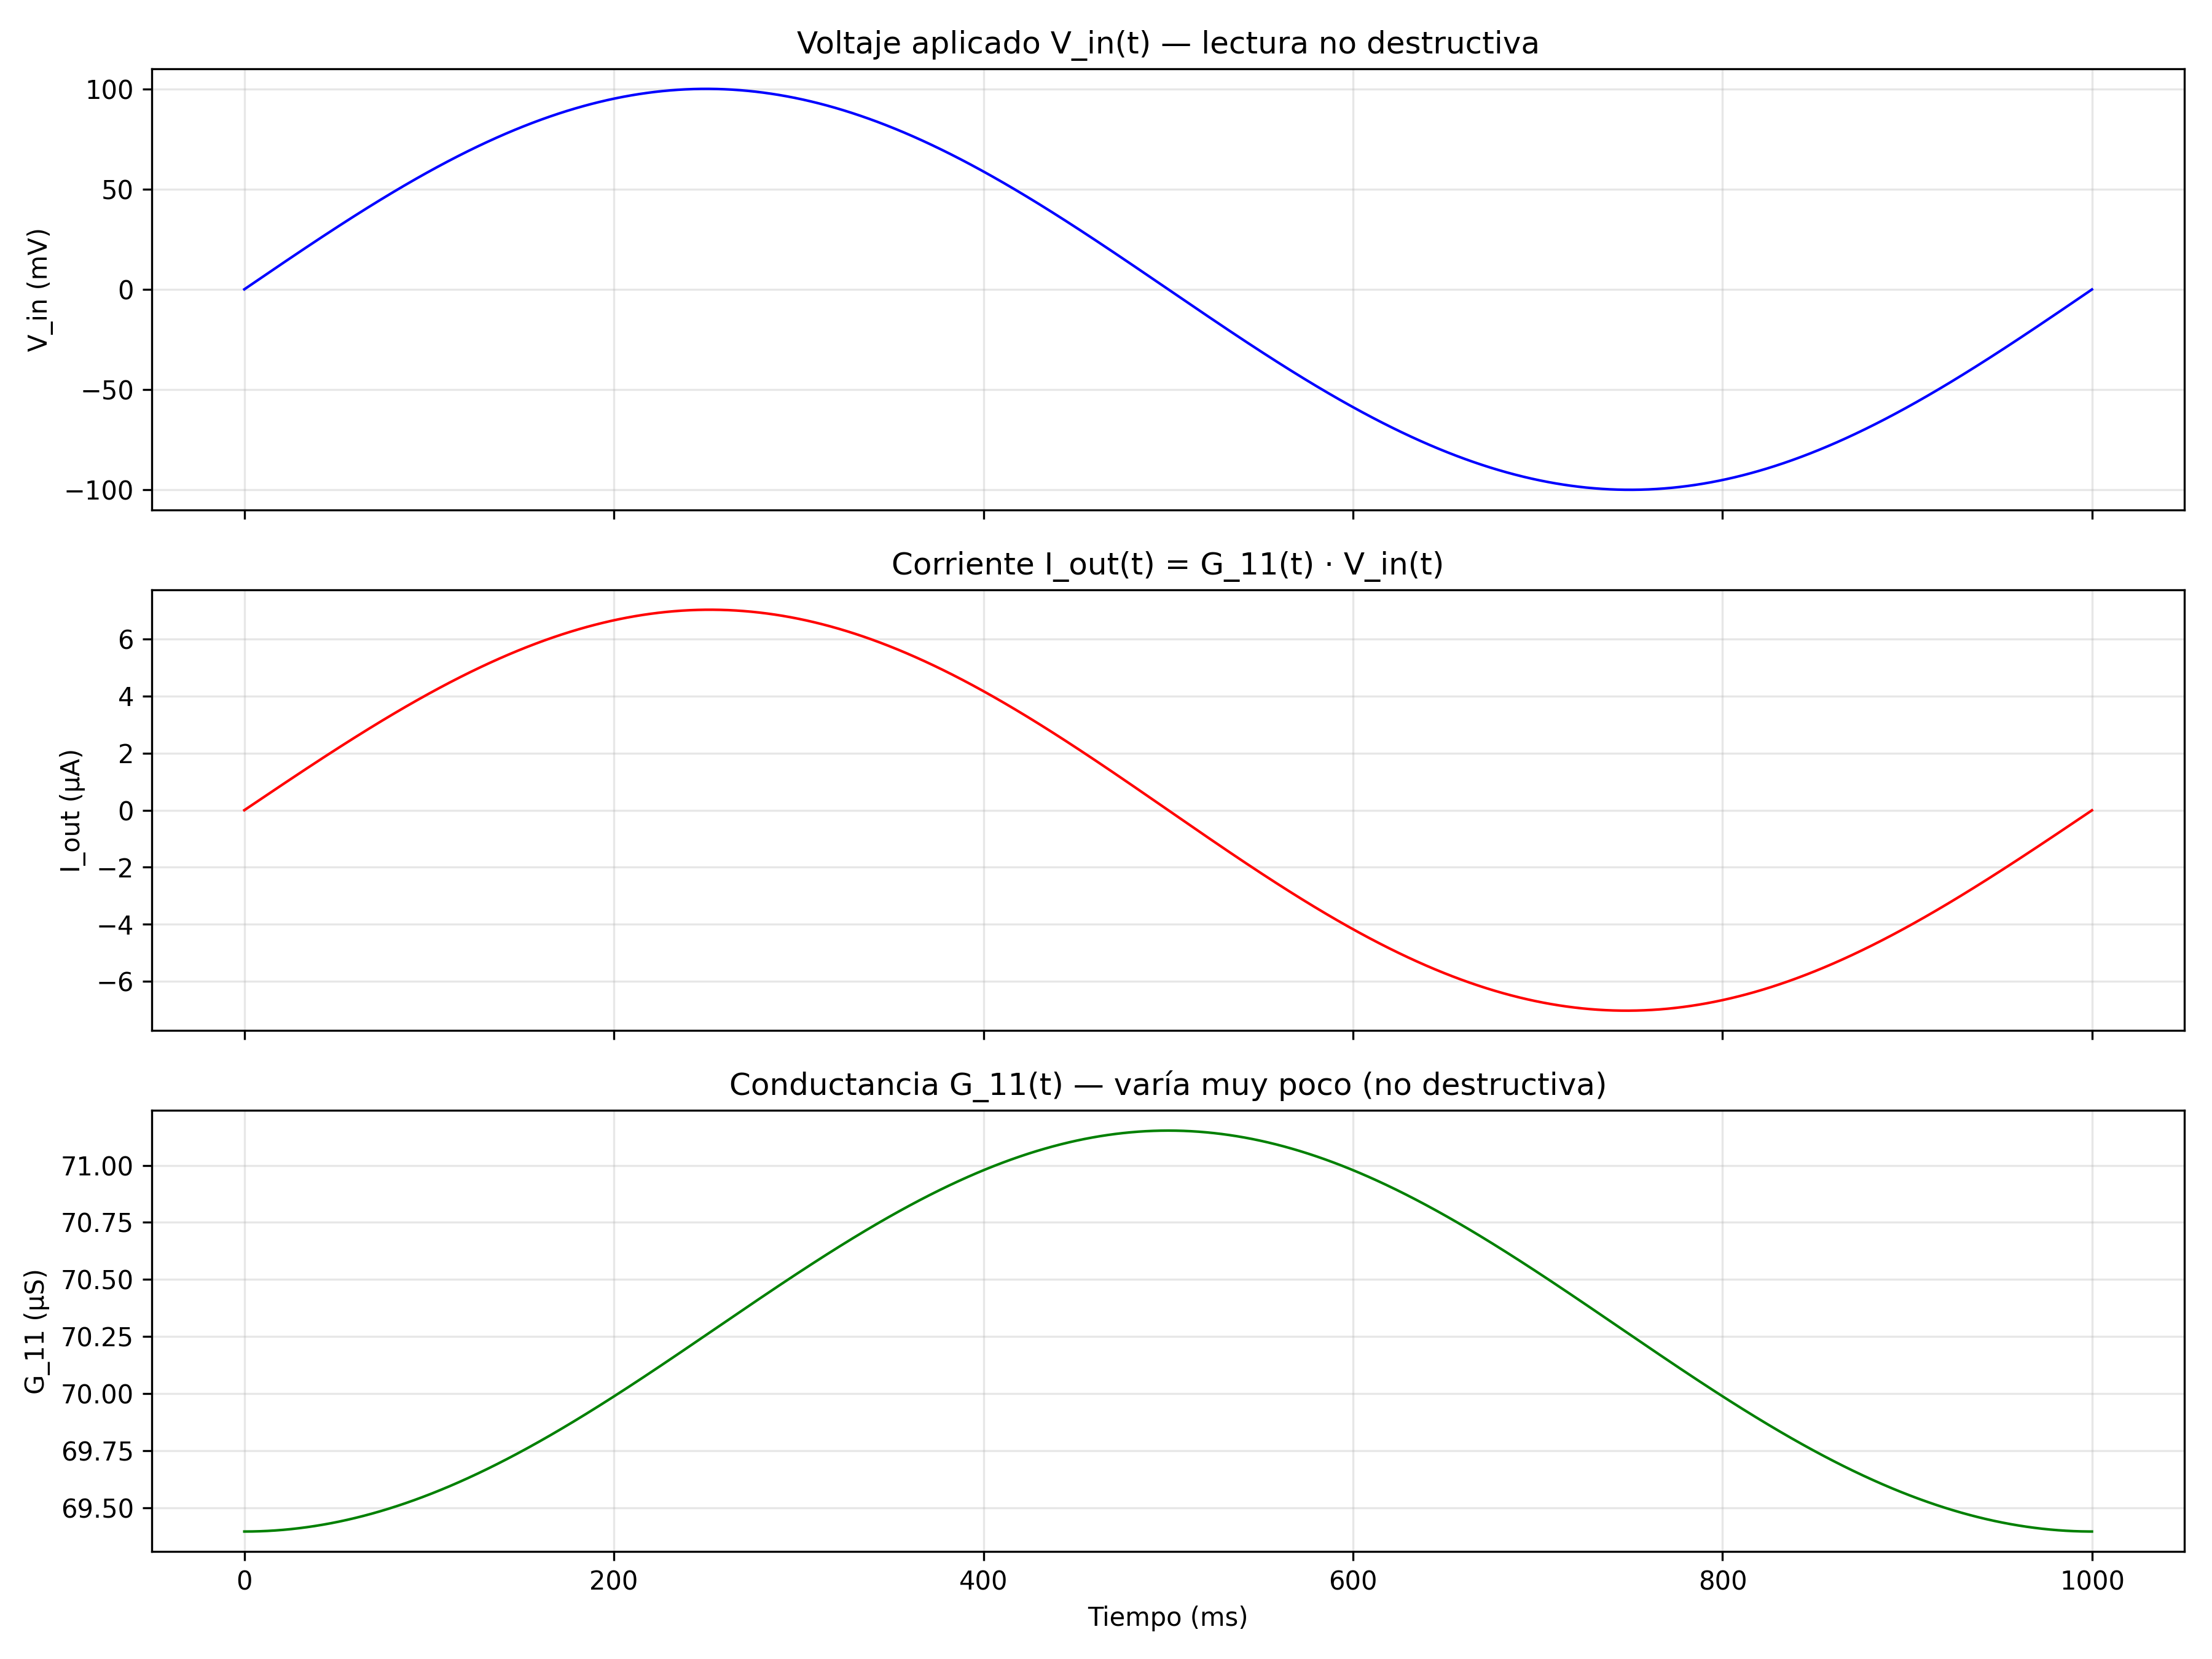
\includegraphics[width=\textwidth]{figuras/fig_21c_crossbar_din.png}
        \caption{Corrientes inferenciales recolectadas $I_j(t)$.}
    \end{subfigure}
    \vskip 0.3cm
    \begin{subfigure}[b]{0.84\textwidth}
        \centering
        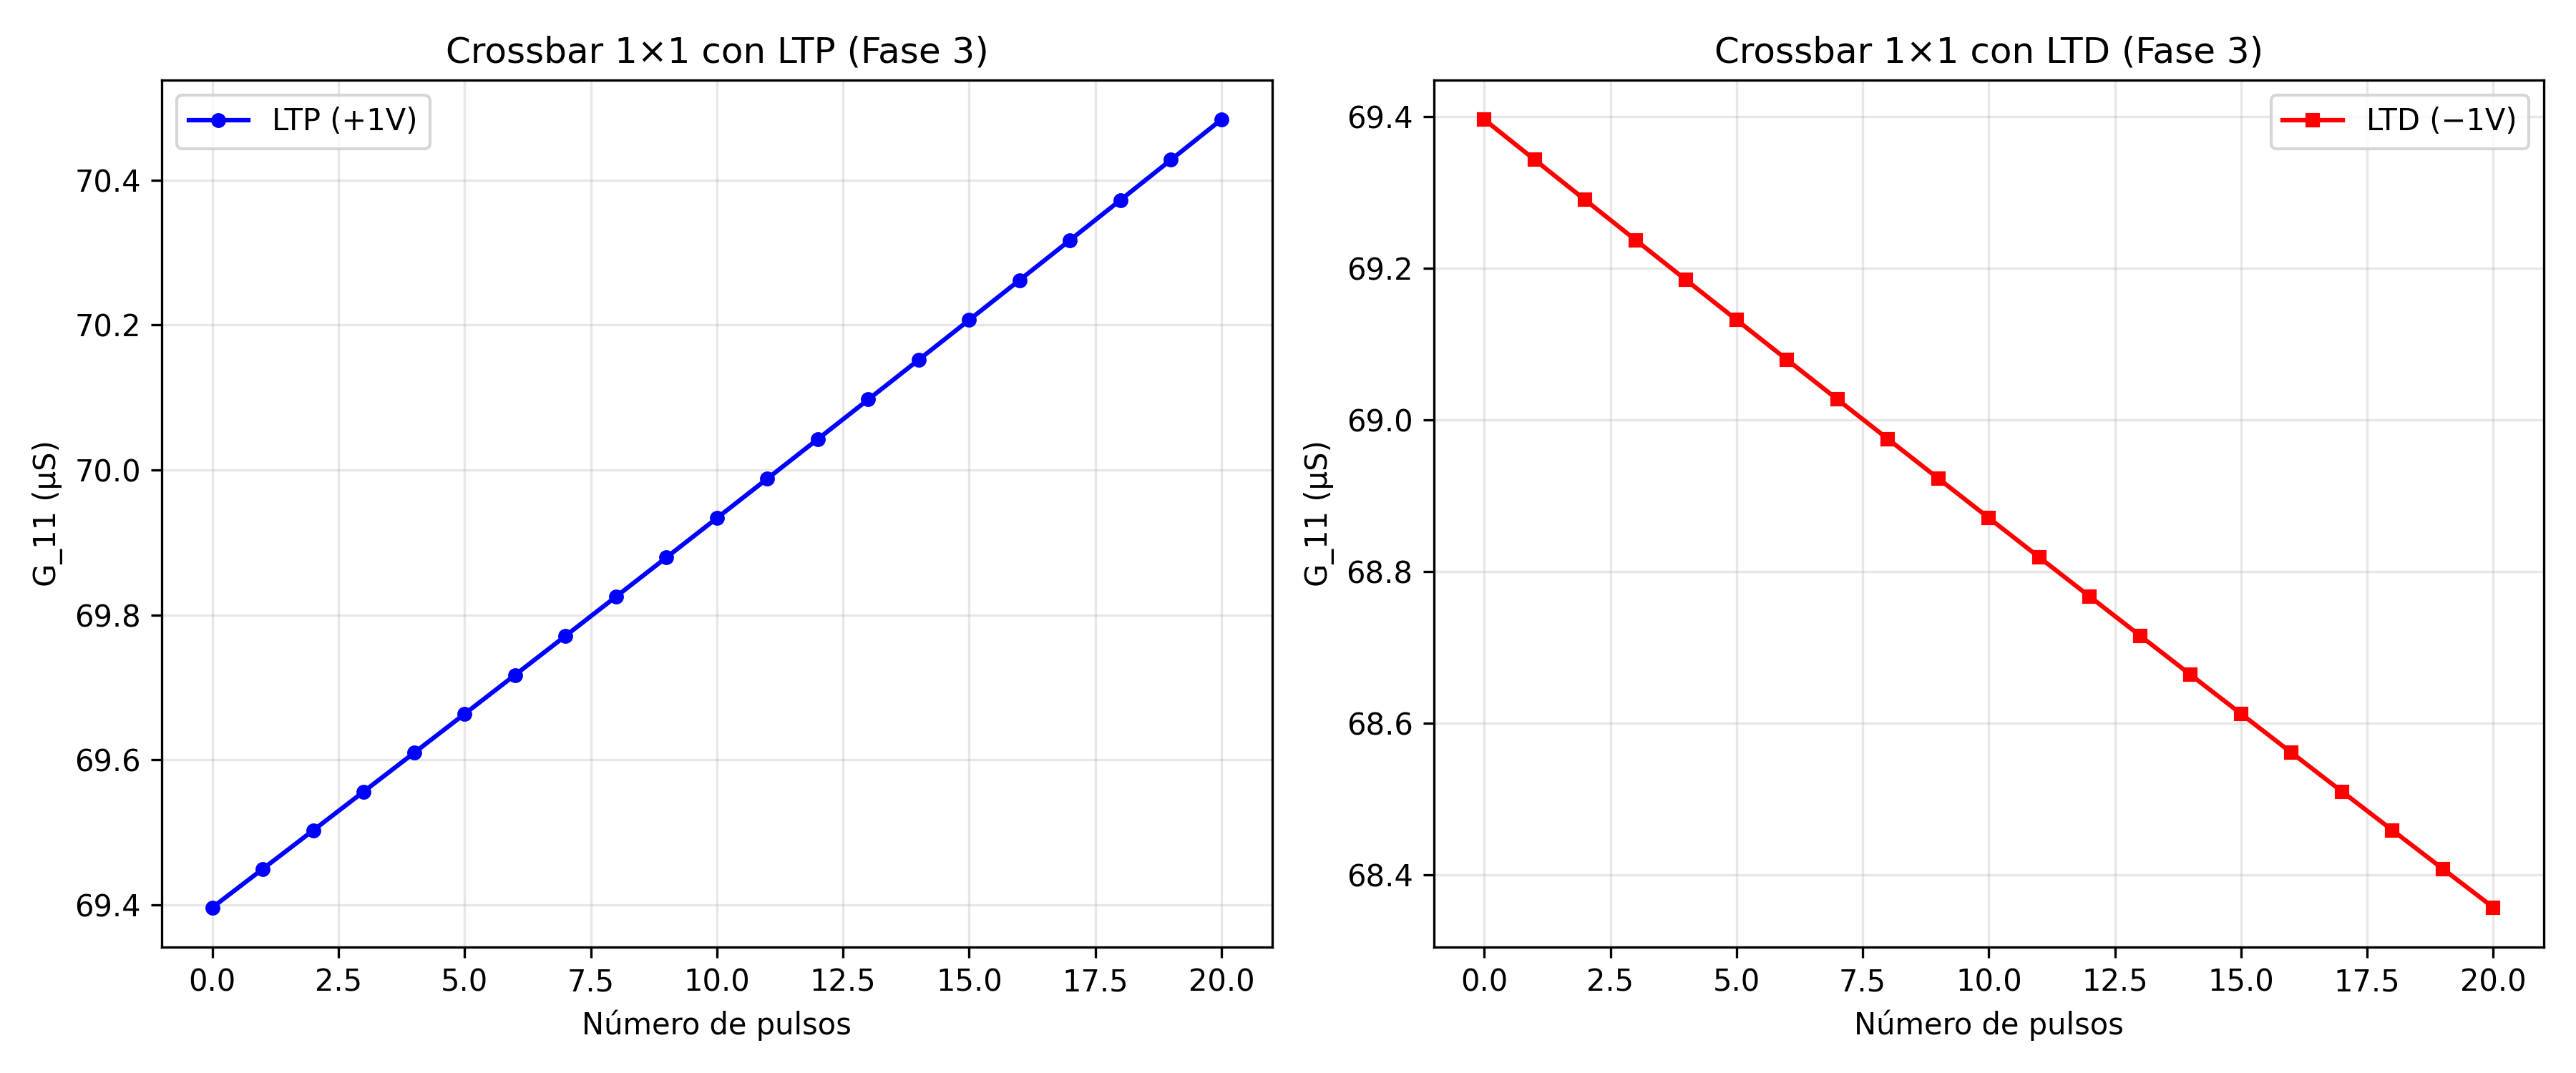
\includegraphics[width=\textwidth]{figuras/fig_21d_crossbar_stdp.png}
        \caption{Cinemática del oscilador memristivo de intersección.}
    \end{subfigure}
    \caption[]{(Continuación; paneles c y d).}
\end{figure}

\textbf{Propósito y Relevancia:} Los cuatro paneles ilustran señales y estados calculados por el modelo de simulación. No demuestran una implementación de hardware ni una ventaja temporal sobre un sistema digital.

\paragraph{Comparación cualitativa con Prezioso et al. (2015)}
La Figura~\ref{fig:prezioso_s3a} compara cualitativamente la forma de las curvas I--V generadas por el modelo local con las curvas representativas de dispositivos del panel S3a de Prezioso et al. (2015)~\cite{31}, correspondiente a la caracterización pre-forming de una porción de un crossbar $10 \times 8$. La comparación es de comportamiento y forma: el generador usa constantes locales y no carga ni digitaliza los puntos experimentales, por lo que no demuestra ajuste numérico ni concordancia punto por punto. Las Figuras~\ref{fig:prezioso_s3bc} muestran una matriz y un histograma sintéticos motivados por los paneles S3b--S3c; no reproducen las mediciones experimentales.

La curva de D-21 es paramétrica. D-22 usa una matriz sintética $4 \times 4$ de conductancias, generada con semilla fija a partir de una media y desviación estándar configuradas en el código. Ninguna de estas dos salidas representa mediciones de celdas reales ni valida ruido térmico o variabilidad medida.

\begin{figure}[H]
    \centering
    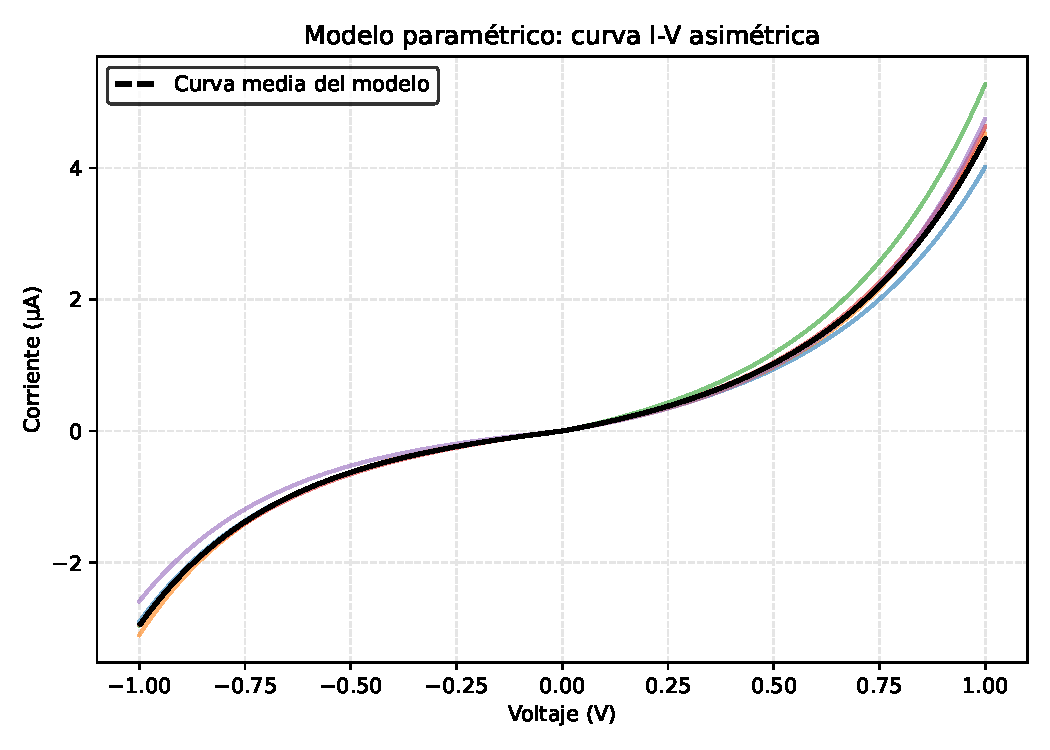
\includegraphics[width=0.85\textwidth]{figuras/23a_prezioso_s3a_modelo_ejemplo.pdf}
    \caption[Comparación cualitativa I-V con Prezioso S3a]{Comparación cualitativa de la forma I--V pre-forming con el panel S3a de Prezioso et al. (2015)~\cite{31}. Las curvas se generan con un modelo paramétrico local; no se cargan puntos digitalizados ni se afirma un ajuste cuantitativo.}
    \label{fig:prezioso_s3a}
\end{figure}

\textbf{Propósito y Relevancia:} Permite comparar visualmente el comportamiento asimétrico no lineal generado localmente con la forma de las curvas representativas del panel S3a. No acredita fidelidad de fabricación, ajuste numérico ni corrientes de fuga medidas.

\begin{figure}[H]
    \centering
    \begin{subfigure}[b]{0.48\textwidth}
        \centering
        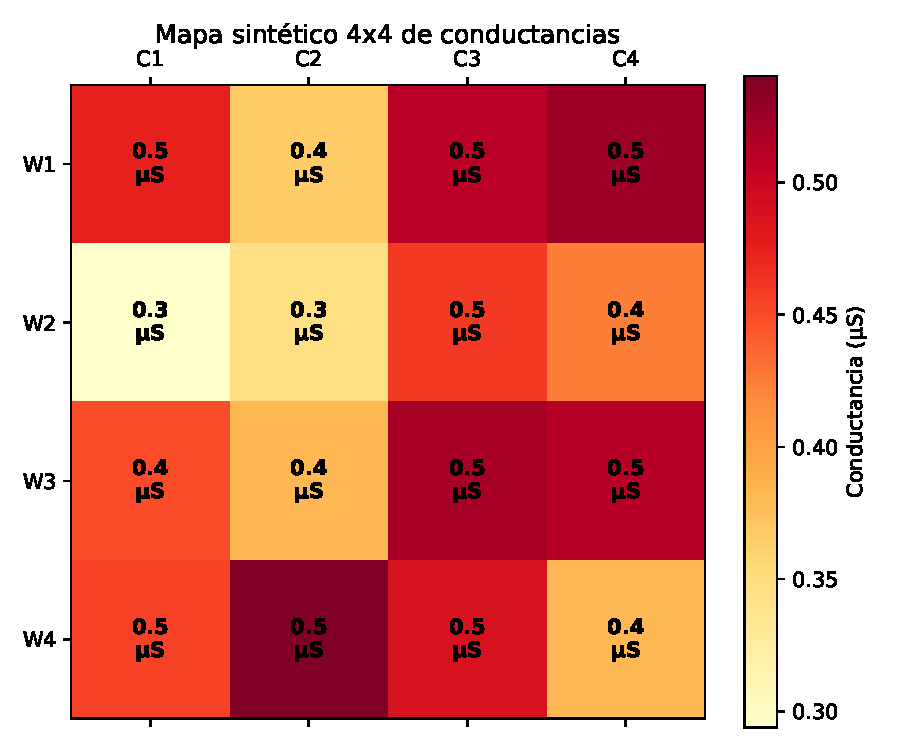
\includegraphics[width=\textwidth]{figuras/23b_prezioso_s3b_modelo_ejemplo.pdf}
        \caption{Matriz sintética de conductancias $4 \times 4$.}
    \end{subfigure}
    \hfill
    \begin{subfigure}[b]{0.48\textwidth}
        \centering
        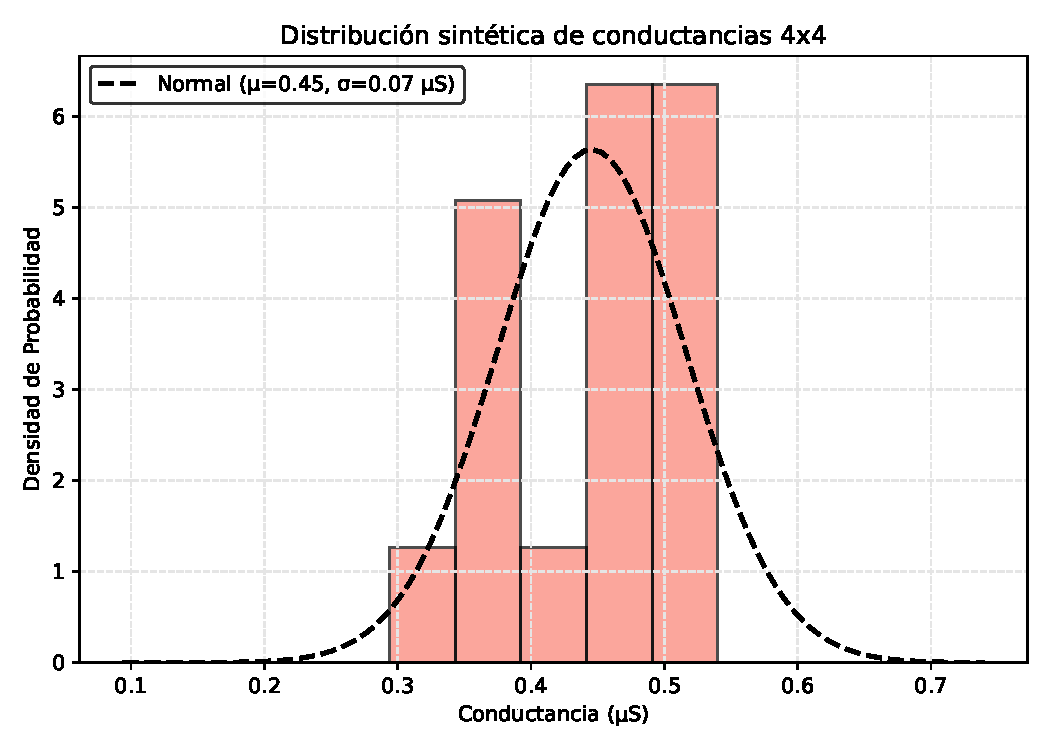
\includegraphics[width=\textwidth]{figuras/23c_prezioso_s3c_modelo_ejemplo.pdf}
        \caption{Histograma de la matriz sintética.}
    \end{subfigure}
    \caption[Ejemplos sintéticos de conductancia]{Ejemplos sintéticos de conductancias en una matriz $4 \times 4$ y su distribución. Los valores se generan en el simulador con semilla fija; no son mediciones ni una reproducción de las Figuras S3b--S3c de Prezioso et al. (2015)~\cite{31}.}
    \label{fig:prezioso_s3bc}
\end{figure}

\textbf{Propósito y Relevancia:} Ilustran la generación de una matriz virtual y un resumen estadístico de sus conductancias. No demuestran que la dispersión del simulador coincida con la variabilidad Device-to-Device del hardware reportado.

\begin{figure}[H]
    \centering
    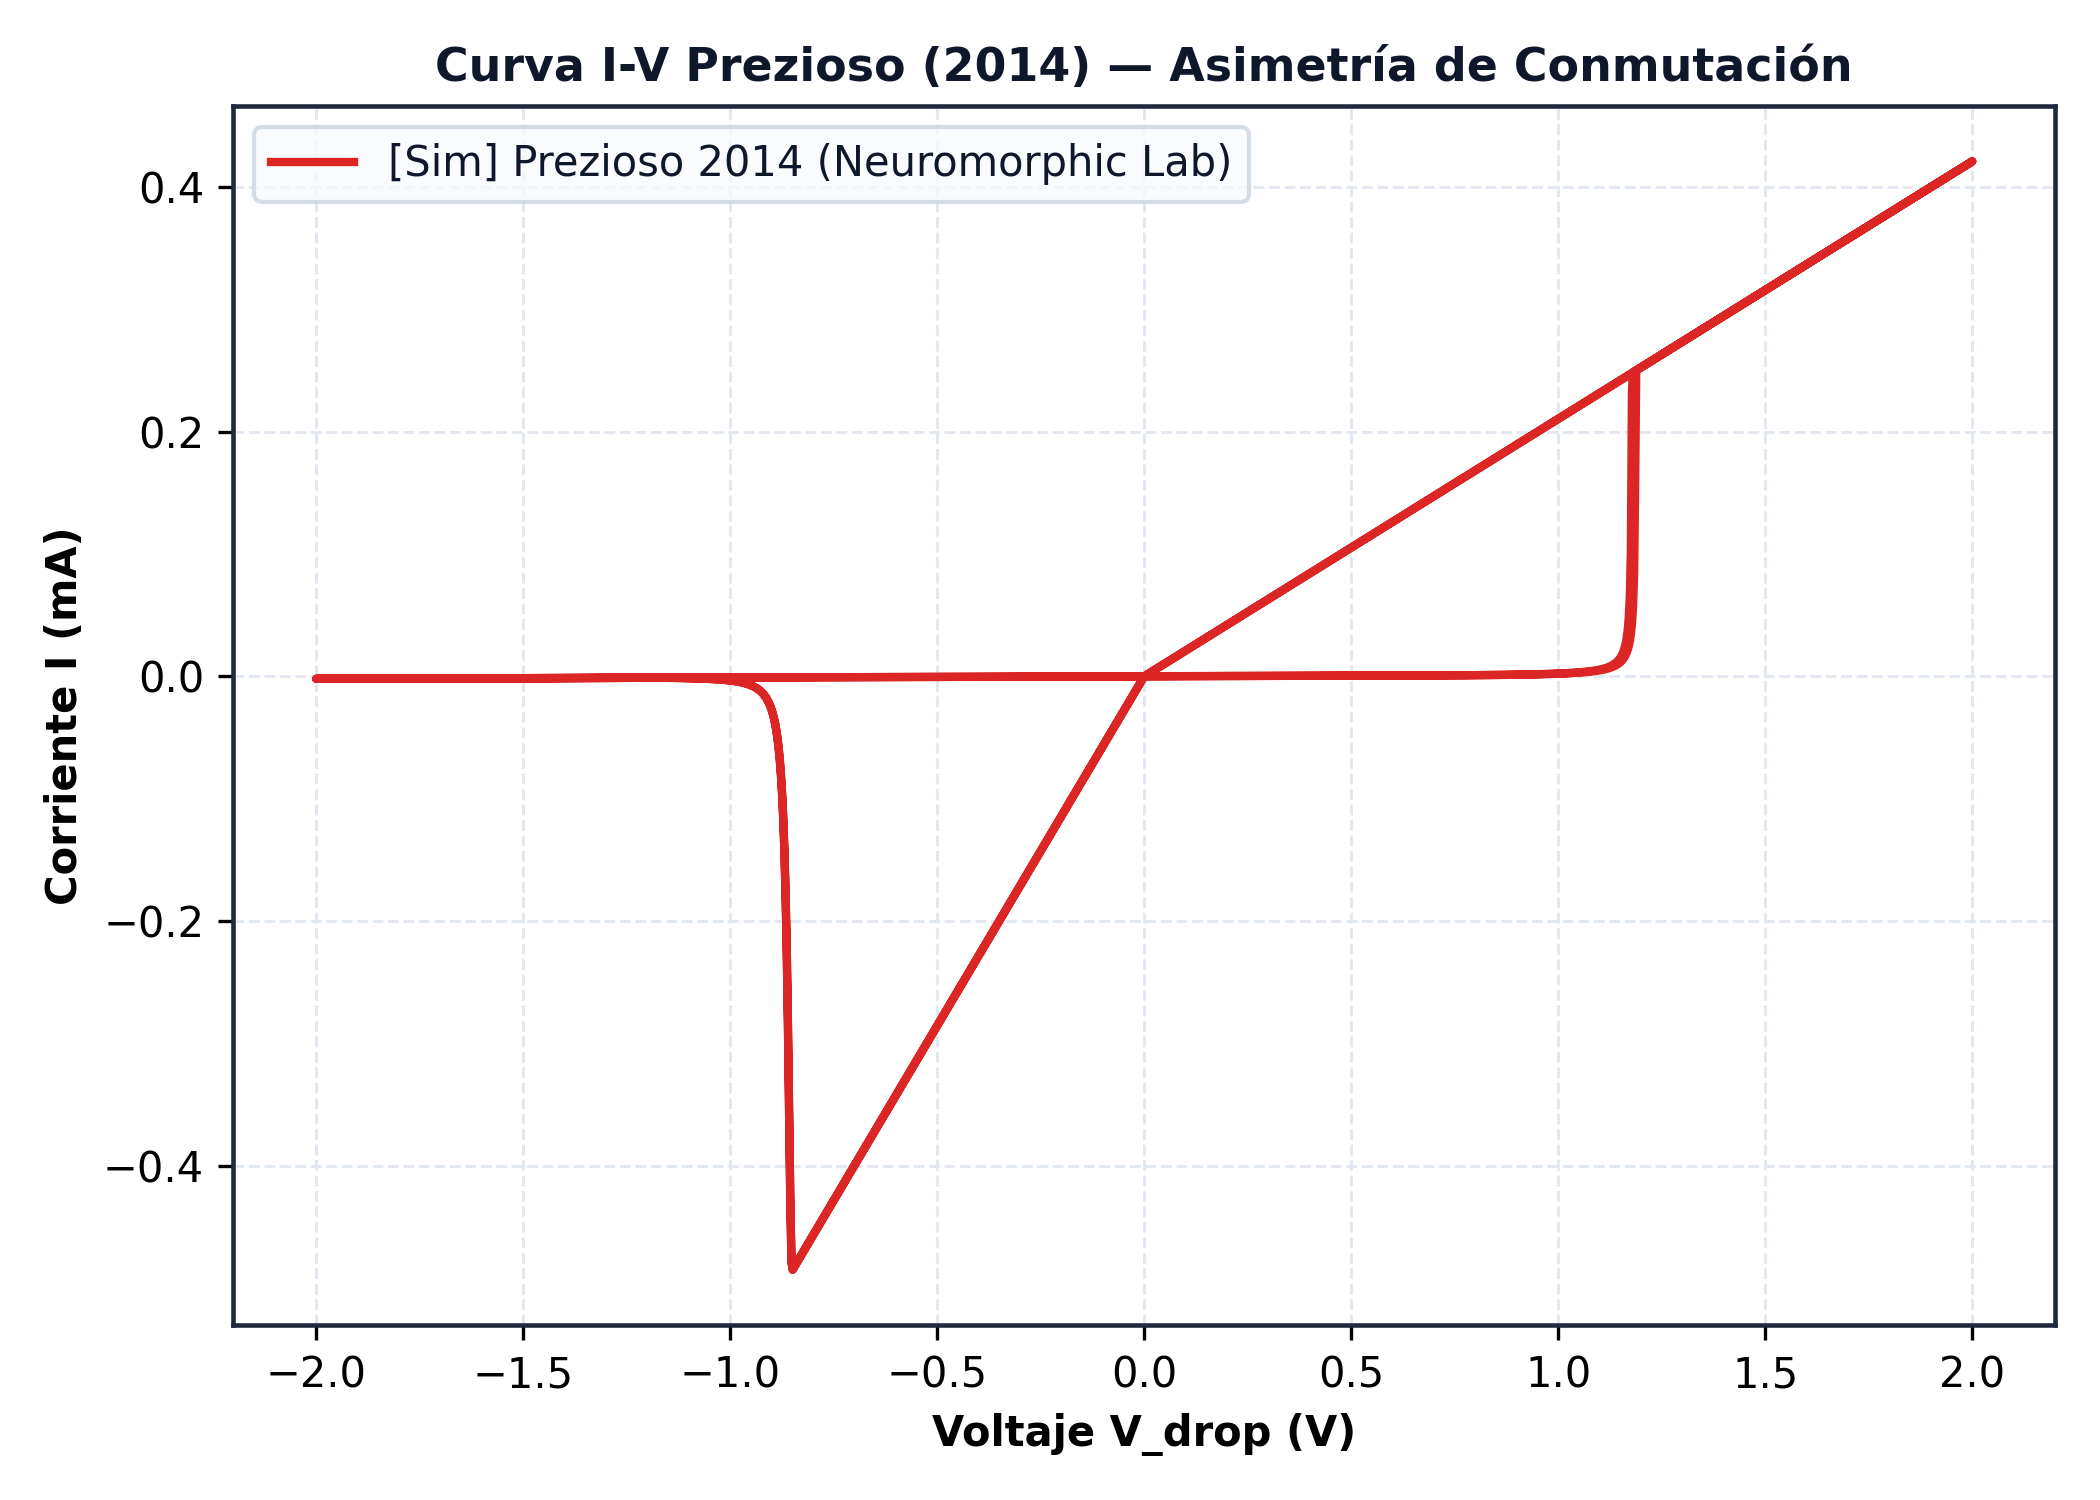
\includegraphics[width=0.7\textwidth]{figuras/fig_22_prezioso_v2.png}
    \caption{Respuesta I--V simulada con el modelo local inspirado en Prezioso et al. (2014)~\cite{3}. La curva se genera con parámetros configurados en el código; no incluye puntos experimentales ni constituye una validación cuantitativa del artículo.}
    \label{fig:22_prezioso_v2}
\end{figure}

\textbf{Propósito y Relevancia:} La figura muestra la respuesta I--V de una simulación local de un dispositivo bajo un barrido de voltaje. No muestra una matriz Crossbar ni prueba integración de sistema, escalamiento, operación SET/RESET en hardware o correspondencia cuantitativa con mediciones del artículo.


% =====================================================================
\subsubsection{Aplicación del crossbar al agente NeuroBot $24 \times 12$}
\label{sec:etapa4_2}

En esta sección se describe una arquitectura de aprendizaje por refuerzo (\textit{Reinforcement Learning}, RL) simulada: una red virtual de $24 \times 12$ acoplada al entorno CartPole. Los resultados son de simulación y no representan una validación experimental en hardware robótico o memristivo.

\paragraph{Arquitectura del Sistema ($24 \times 12$)}
El cerebro neuromórfico del agente consiste en un crossbar memristivo de $N=24$ filas de entrada y $M=12$ columnas de salida.

\subparagraph{Codificador de Estados (Encoder Top-K)}
El vector de observación continuo $\mathbf{s} = [x, \dot{x}, \theta, \dot{\theta}] \in \mathbb{R}^4$ se proyecta mediante una batería de receptores gaussianos distribuidos a lo largo del dominio de cada variable. Se aplica un mecanismo Top-K ($K=10$) que selecciona las 10 filas de mayor activación, generando un patrón binario disperso de voltajes de lectura $V_{\text{rows}} \in \{0, V_{\text{read}}\}$.

\subparagraph{Crossbar Memristivo y Solución Nodal (MNA)}
La corriente integrada por columna $\mathbf{I}_{\text{col}} \in \mathbb{R}^{12}$ se calcula resolviendo la matriz MNA con resistencia de línea $R_{\text{wire}} = 10^{-3}\,\Omega$ y resistencia de sensado $R_{\text{sense}} = 100\,\Omega$:
\begin{equation}
    \mathbf{I}_{\text{col}} = \text{MNA}(\mathbf{G}, V_{\text{rows}}, R_{\text{wire}}, R_{\text{sense}})
\end{equation}
donde $G_{ij} = \frac{1}{R_{\text{on}} + X_{ij}(R_{\text{off}} - R_{\text{on}})}$ representa la conductancia de la celda en el estado interno $X_{ij} \in [0, 1]$.

\subparagraph{Decodificador y Acción (Softmax e Inercia de Motor)}
Las 12 columnas se agrupan en pares de conductancias asociadas a 6 niveles discretos de fuerza activa para giro hacia la izquierda ($1 - 30\,\text{N}$) y 6 para la derecha ($1 - 30\,\text{N}$). La probabilidad de selección de acción $\pi_j$ sigue una distribución Softmax parametrizada por la temperatura ambiental $T$:
\begin{equation}
    \pi_j = \frac{\exp(I_j / T)}{\sum_{k=1}^M \exp(I_k / T)}
\end{equation}
Se aplica una tasa de cambio (slew rate) de $50/50$ en la dinámica del actuador para simular la inercia del motor robótico real.

\paragraph{REINFORCE con baseline}
El aprendizaje del agente no es STDP: es REINFORCE con baseline y ocurre al final de cada episodio:
\begin{equation}
    \Delta X_{ij} = -\eta \cdot E_{ij} \cdot (R_{\text{ep}} - b)
\end{equation}
donde $E_{ij}$ es la elegibilidad acumulada por paso a partir de $\mathrm{pre}_i(t)(\mathbf{1}_{j=a(t)}-\pi_j(t))$, con decaimiento $\gamma$ entre pasos. No se usa una ventana de STDP entre disparos pre y postsinápticos ni una traza de memristores volátiles; $E$ se mantiene como acumulador matemático del agente.

Con la convención $X=1-x$, una ventaja positiva produce
$\Delta X<0$ en la columna elegida cuando su elegibilidad es positiva;
esto reduce su resistencia y aumenta su conductancia. La prueba
unitaria del agente comprueba este signo en un caso controlado, sin
demostrar convergencia general ni equivalencia con STDP.

La actualización $\Delta X$ utiliza recorte por norma de gradiente
($\max|\Delta X| \le 0.05$) y se congela si
$R_{\text{ep}} \ge 430$. Este umbral es un criterio operativo del
protocolo evaluado y no demuestra que la política alcanzada sea óptima.

\paragraph{Resultados de simulación y discusión en control robótico}

Los valores de recompensa y ablación de esta sección proceden de
registros de simulación previamente reportados. No se reejecutaron las
cinco semillas ni las ablaciones durante esta revisión; por tanto, se
presentan como resultados reportados, no como cifras reproducidas aquí
ni como resultados experimentales de hardware.

\subparagraph{Convergencia y Reproducibilidad Multi-Semilla}
Se ejecutaron cinco semillas (0--4), con 300 episodios cada una, $V_{\mathrm{read}}=0.05$ V, D2D ($\sigma=0.08$), C2C ($\sigma=0.05$, $\theta=1\,\mathrm{s}^{-1}$, $dt=0.02\,\mathrm{s}$) y congelamiento de la actualización de pesos para $R_{\mathrm{ep}}\geq430$. Las recompensas medias de los últimos 200 episodios fueron 369.66, 421.44, 474.31, 462.79 y 448.36, respectivamente; la media entre semillas fue 435.31 y su desviación estándar 37.28. Cuatro corridas alcanzaron al menos una recompensa episódica de 480; la semilla 3 tuvo máximo 479.14. Los registros se guardan como \texttt{run\_24x12\_A\_d2d\_c2c\_seed0.json}--\texttt{seed4.json}; la figura y discusión se presentan en la Sección~3.4.1.

La media de la semilla 0 debe interpretarse considerando su trayectoria:
las recompensas medias por bloques de 50 episodios fueron 13.90,
58.55, 99.39, 470.69, 461.27 y 447.29. Su primera media móvil de
20 episodios que alcanzó 430 apareció en el episodio 157. Así, el
promedio de los episodios 101--300 (369.66) refleja en buena medida el
tiempo que tardó esta corrida en alcanzar recompensas altas y no basta
para concluir que la semilla sea intrínsecamente peor. Este cruce es
un indicador operativo de adquisición de desempeño, no una
demostración formal de convergencia; el análisis detallado se presenta
en la Sección~\ref{sec:res_cartpole}.

\subparagraph{Estudio de Ablaciones}
Para validar la contribución de cada bloque del agente, se evaluaron cuatro configuraciones (Figura~\ref{fig:ablaciones_robot}):
\begin{itemize}
    \item \textbf{A (Control Base):} Sistema completo con decaimiento térmico y traza acumulativa ($\bar{R} \approx 491.9$ en semillas exitosas, $60\%$ de tasa de convergencia en 5 semillas aleatorias).
    \item \textbf{B (Sin Adaptación Térmica, $T=0.10$ Fijo):} Colapso por congelamiento estocástico ($\bar{R} = -39.0$). Demuestra que sin alta exploración inicial, el agente congela la búsqueda de políticas.
    \item \textbf{C (Sin Traza de Elegibilidad, $\varepsilon=0$):} Colapso total ($\bar{R} = -33.3$, $\Delta X=0$), evidenciando que la elegibilidad acumulada es necesaria en la configuración REINFORCE evaluada.
    \item \textbf{D (Hebbiano Sin Modulación $R_{\text{ep}}-b$):} Divergencia y colapso ($\bar{R} = -39.0$) por falta del escalar de refuerzo global.
\end{itemize}

\begin{figure}[H]
    \centering
    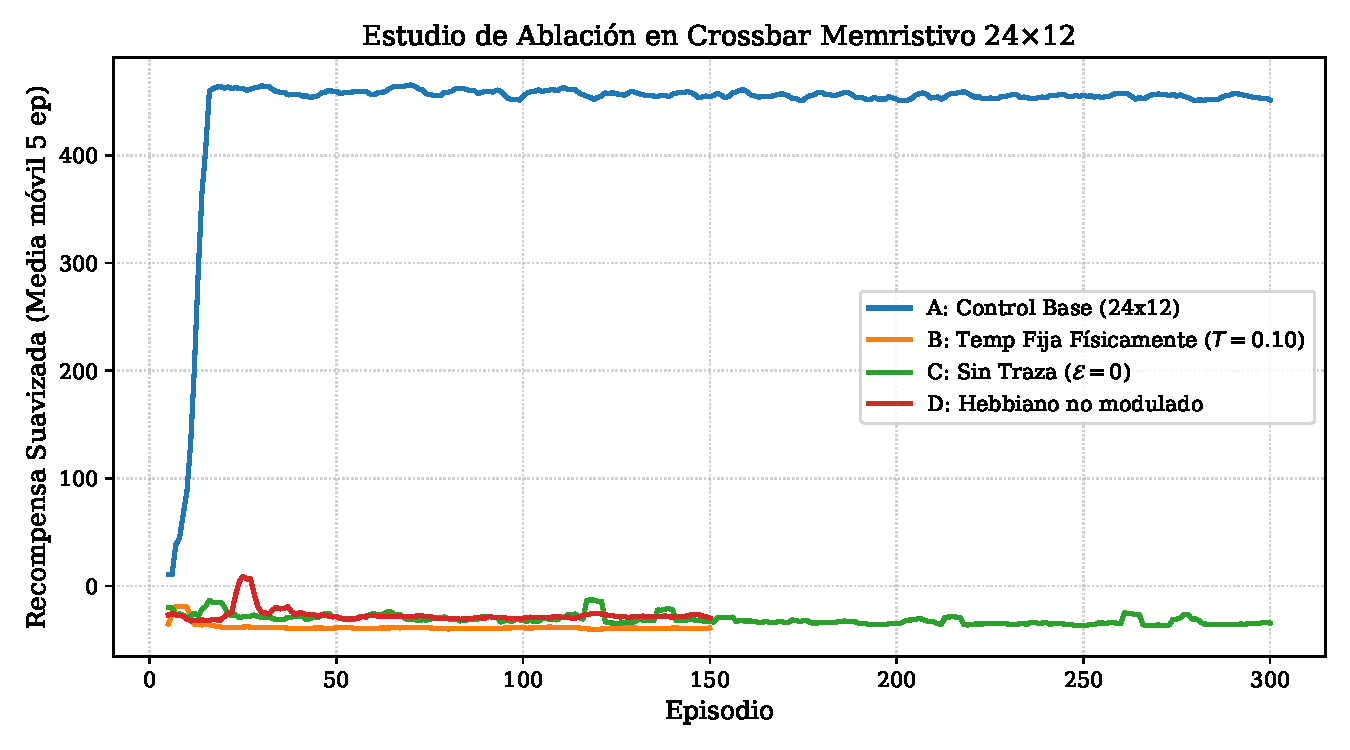
\includegraphics[width=0.85\textwidth]{figuras/comparativa_ablaciones_24x12.pdf}
    \caption{Estudio de ablación comparativo (A, B, C, D) en el crossbar $24 \times 12$.}
    \label{fig:ablaciones_robot}
\end{figure}

\subparagraph{Heatmap de la Matriz Memristiva Consolidada ($X$)}
La Figura~\ref{fig:heatmap_robot} muestra la distribución final del estado memristivo $X \in [0, 1]$. Se observa una estructura bimodal no saturada ($\mu = 0.165, \sigma = 0.118$) con bandas claras de activación sináptica diferenciadas por la velocidad y el ángulo del poste.

\begin{figure}[H]
    \centering
    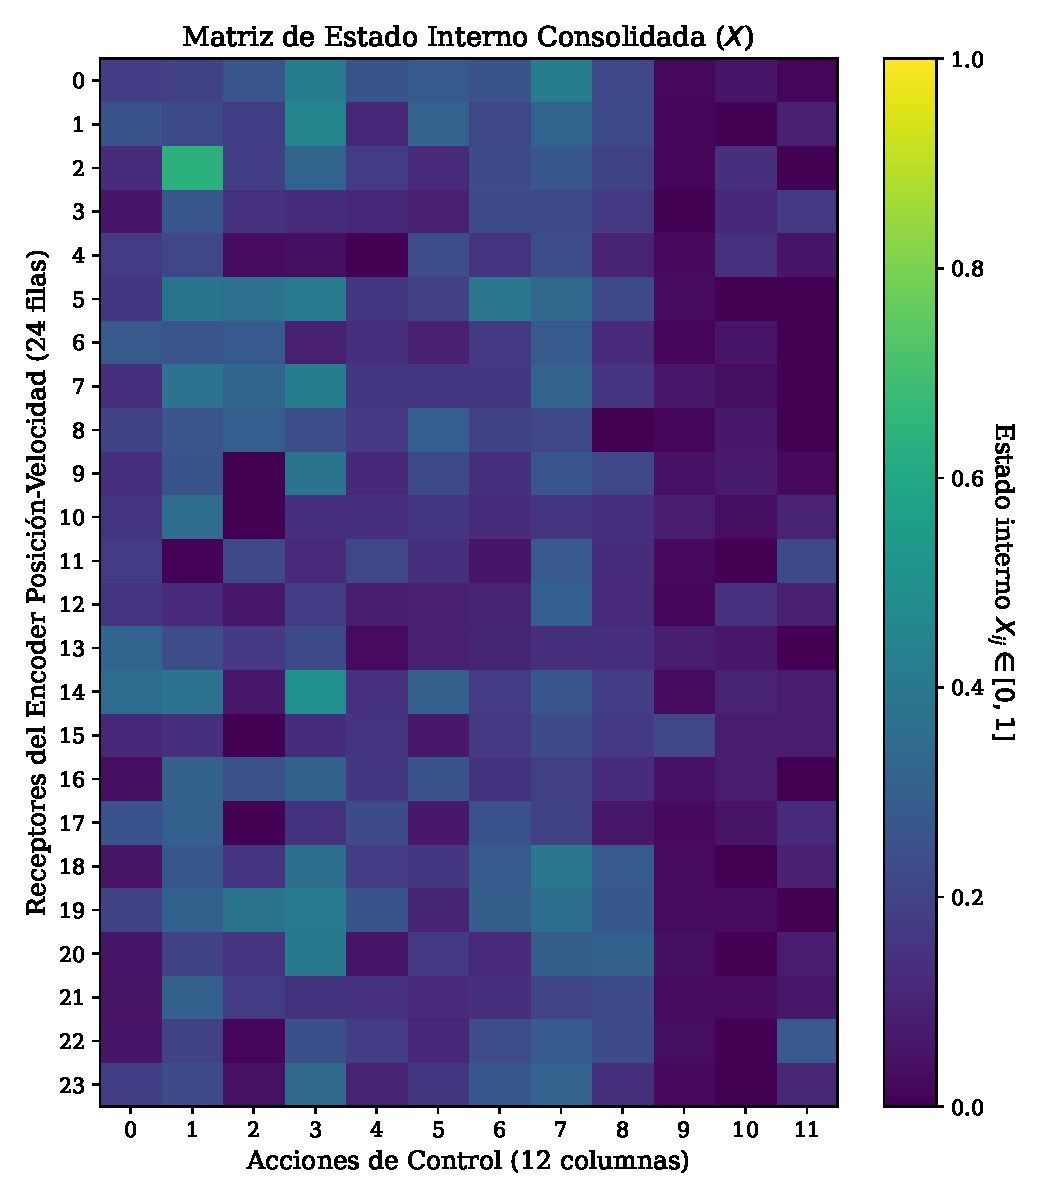
\includegraphics[width=0.65\textwidth]{figuras/heatmap_matriz_X_24x12.pdf}
    \caption{Heatmap de la variable de estado interno $X$ tras el entrenamiento del agente; la conductancia $G$ se deriva de $X$ y no se muestra en esta figura.}
    \label{fig:heatmap_robot}
\end{figure}


% =====================================================================
\subsubsection{Validación del Modelo Físico del Crossbar (Suite de 10 Experimentos)}
\label{sec:suite_10_exp}

La suite consta de 10 experimentos de simulación autónomos del modelo
crossbar. Las cifras que siguen son las consignadas en sus informes y
figuras existentes; no se reejecutaron ni se verificaron de nuevo sus
registros de entrada en esta revisión. Por ello describen resultados
reportados del modelo, no una certificación de fidelidad respecto a
hardware real. Las condiciones de excitación y las impedancias de
sensado ($R_{\text{sense}} = 100\,\Omega$) se atribuyen a la
configuración declarada para el agente.

\paragraph{Exp.~1 --- Error de lectura del crossbar vs.\ tamaño}

La Figura~\ref{fig:exp01} cuantifica el error relativo de lectura del arreglo
al escalar de $N=4$ a $N=32$ filas con $M=12$ columnas fijas. Se define el
error relativo como
$\varepsilon = \|I_{\text{col}} - I_{\text{ideal}}\| / \|I_{\text{ideal}}\|$,
donde $I_{\text{col}}$ es la solución nodal del arreglo (MNA con
$R_{\text{wire}}$ y $R_{\text{sense}}$) e $I_{\text{ideal}} = \mathbf{G}^T \mathbf{V}$
es la proyección lineal ideal.

Para $N=4$ el error es $\varepsilon \approx 6.5\%$ y escala monótonamente
hasta $\varepsilon \approx 41\%$ para $N=32$. Este crecimiento refleja la
contribución conjunta de la caída resistiva en las líneas ($R_{\text{wire}}$)
y el divisor formado por $R_{\text{sense}}$ con la conductancia agregada del
arreglo. El efecto de corrientes parásitas estrictas (\textit{sneak paths} en
el sentido clásico: fila única activa con filas flotantes) requiere una
configuración de excitación distinta y se considera una extensión natural
para trabajos futuros.

\begin{figure}[H]
  \centering
  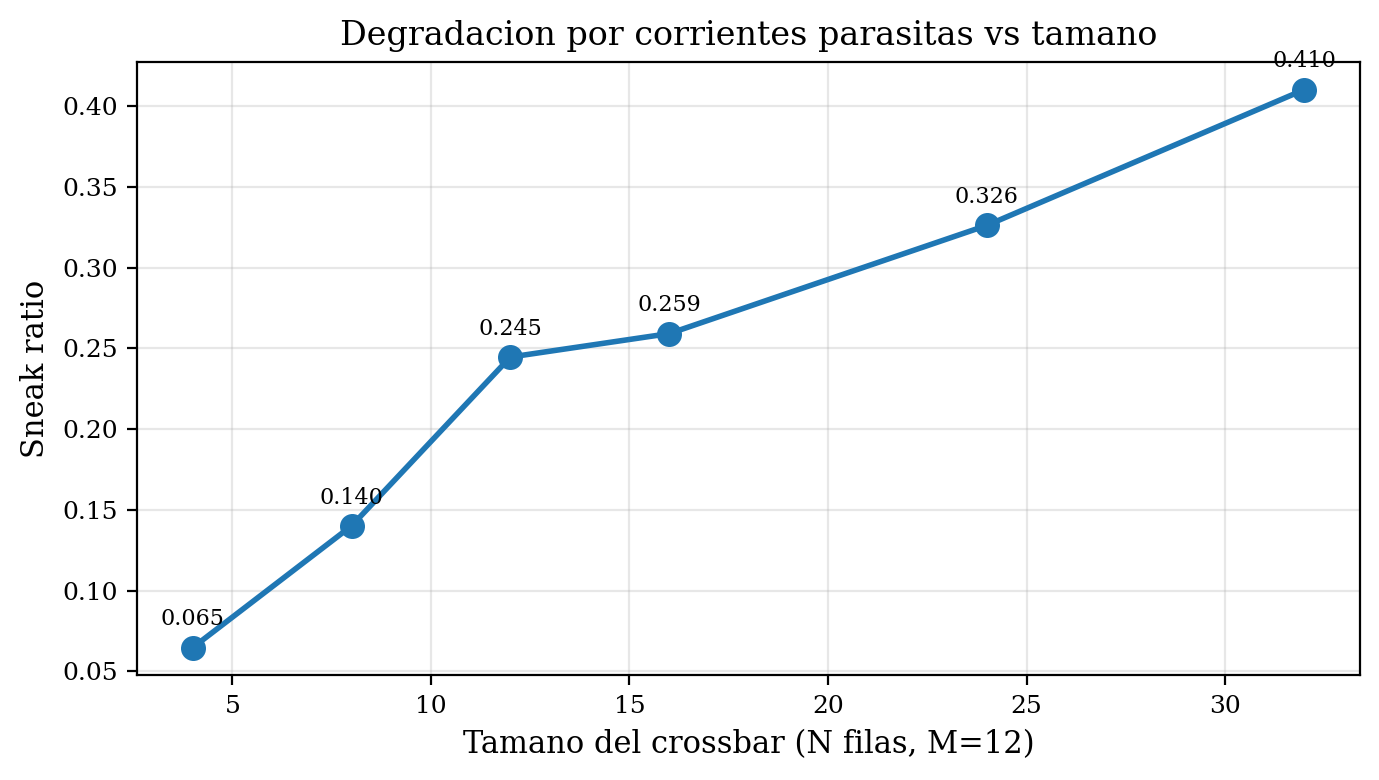
\includegraphics[width=0.65\textwidth]{experiments/figures/exp01_sneak_vs_N.png}
  \caption{Error relativo de lectura vs.\ tamaño del arreglo. Crecimiento
  monótono desde $N=4$ ($6.5\%$) hasta $N=32$ ($41\%$).}
  \label{fig:exp01}
\end{figure}

\paragraph{Exp.~2 --- MNA real vs.\ modelo ideal}
La Figura~\ref{fig:exp02} compara corrientes MNA e ideales para cuatro tamaños. En el caso $N=24$, el error medio por componente alcanza $29.08\%$, reflejando la contribución acumulada de $R_{\text{wire}}$ y $R_{\text{sense}}$ sobre las corrientes de columna.
\begin{figure}[H]
  \centering
  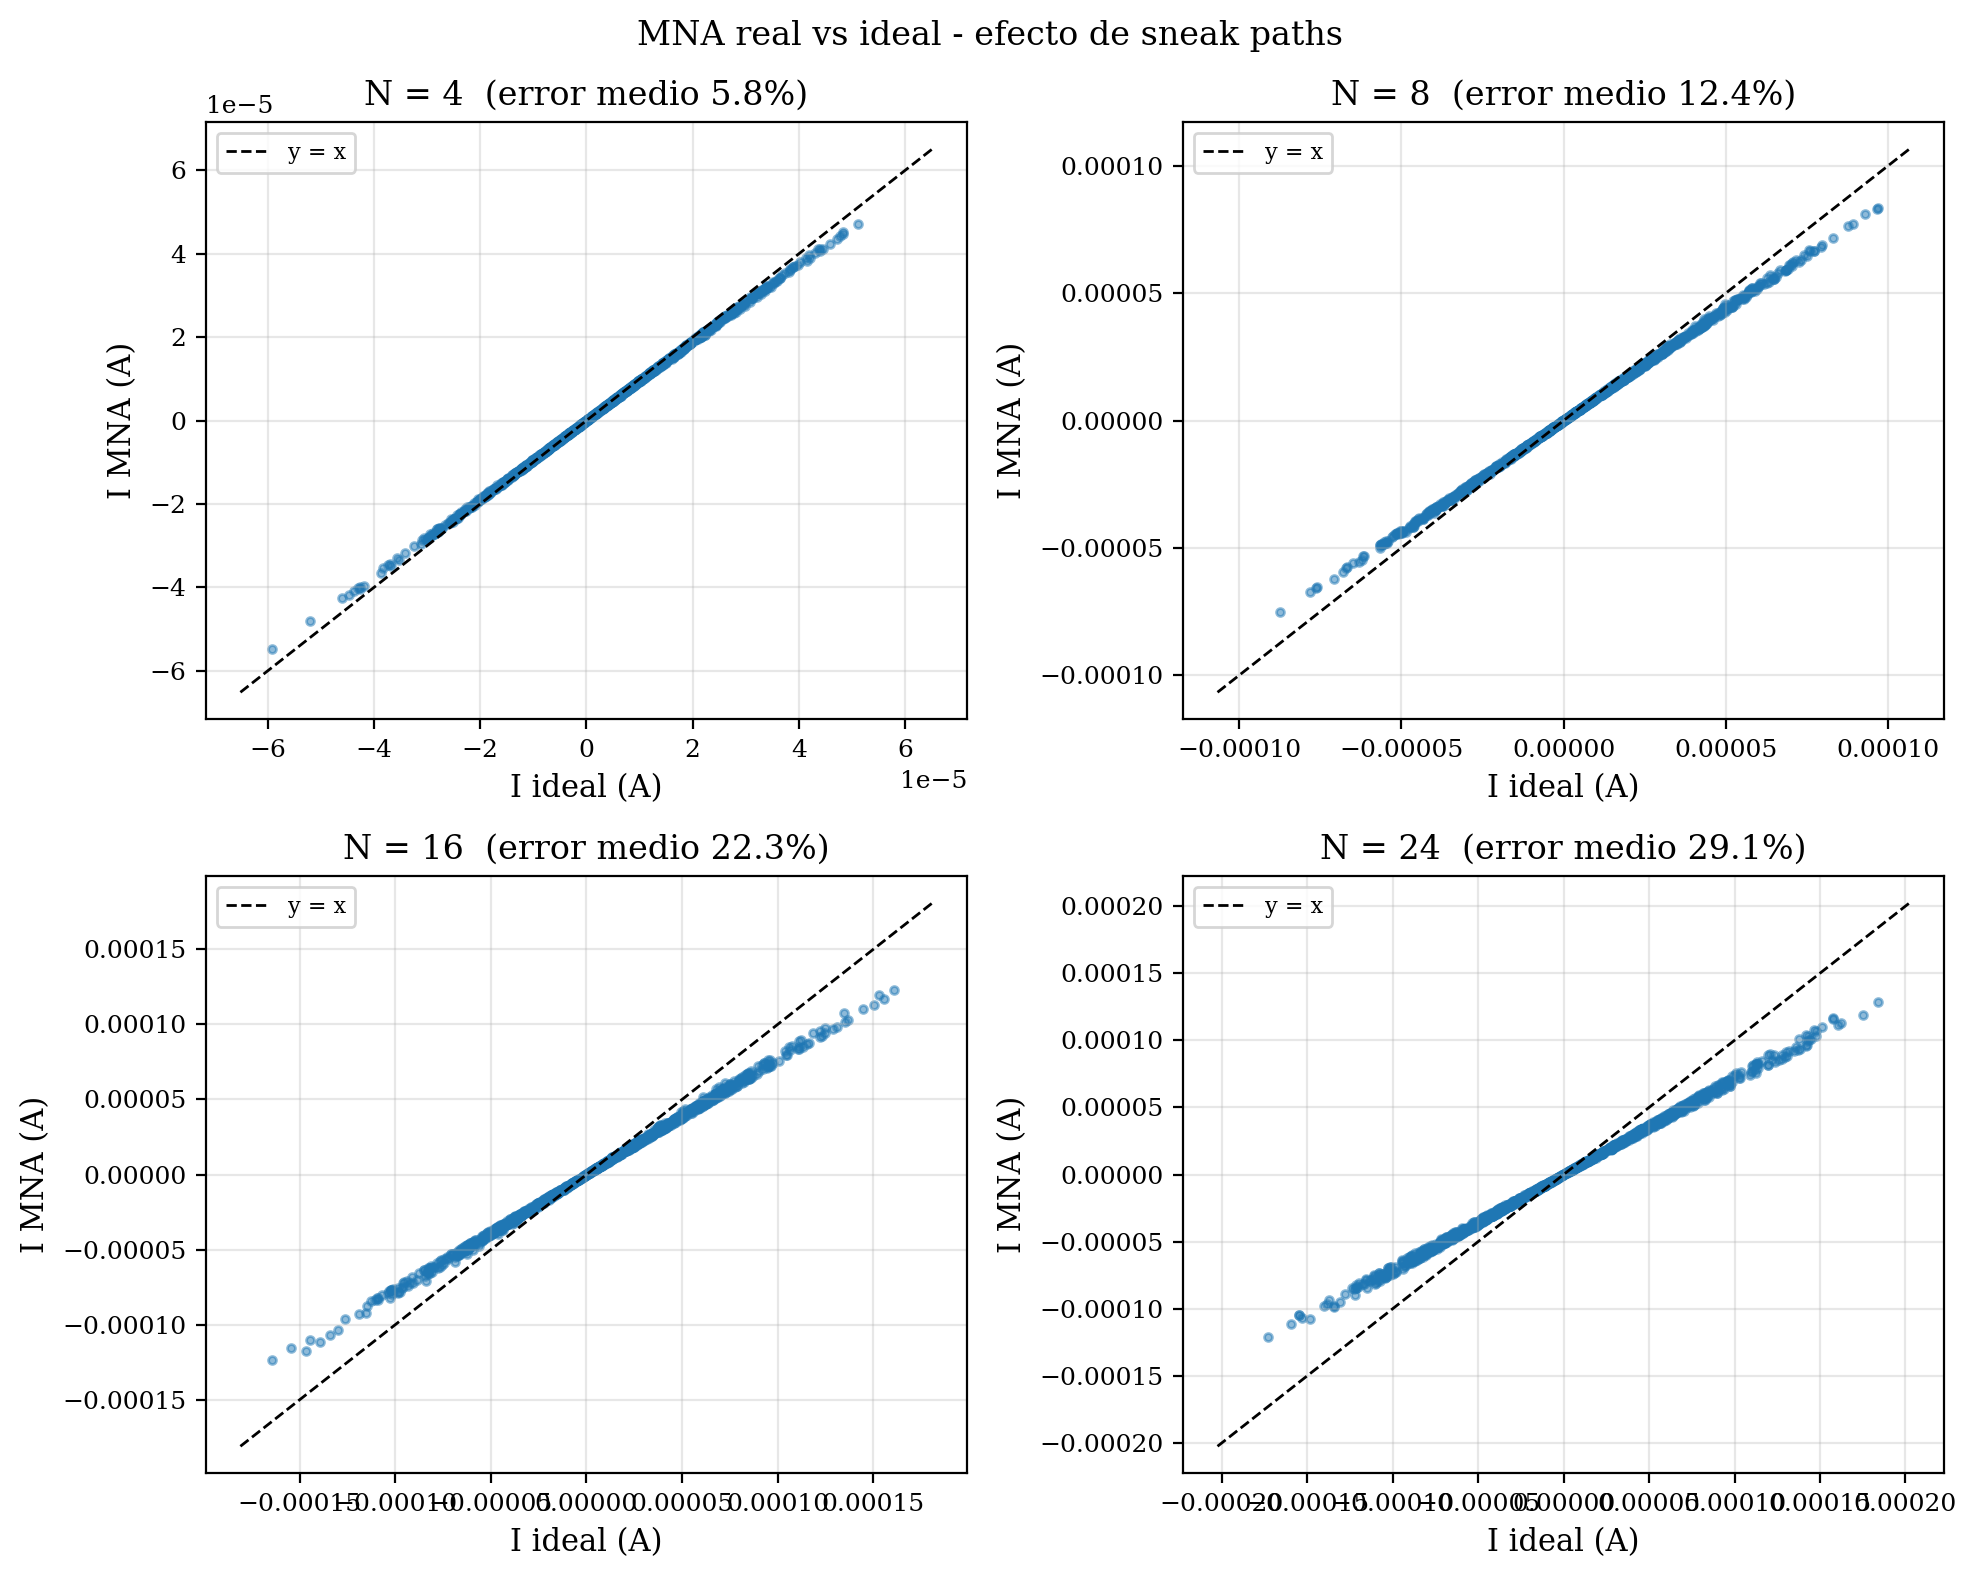
\includegraphics[width=0.90\textwidth]{experiments/figures/exp02_mna_vs_ideal.png}
  \caption{Diagrama de dispersión MNA vs.\ Ideal. El error crece de forma no lineal con $N$.}
  \label{fig:exp02}
\end{figure}

\paragraph{Exp.~3 --- Caída de tensión en línea ($R_{\text{wire}}$)}
La Figura~\ref{fig:exp03} ilustra cómo $R_{\text{wire}}$ distorsiona el perfil de corriente. El efecto sobre el perfil es doble: atenúa la corriente media ($-13\%$ entre $R_{\text{wire}} = 1\,\text{m}\Omega$ y $R_{\text{wire}} = 10\,\Omega$) y mantiene prácticamente invariante la no-uniformidad relativa entre columnas ($\sim 27\%$), dominada por la dispersión dispositivo-a-dispositivo de $\mathbf{G}$.
\begin{figure}[H]
  \centering
  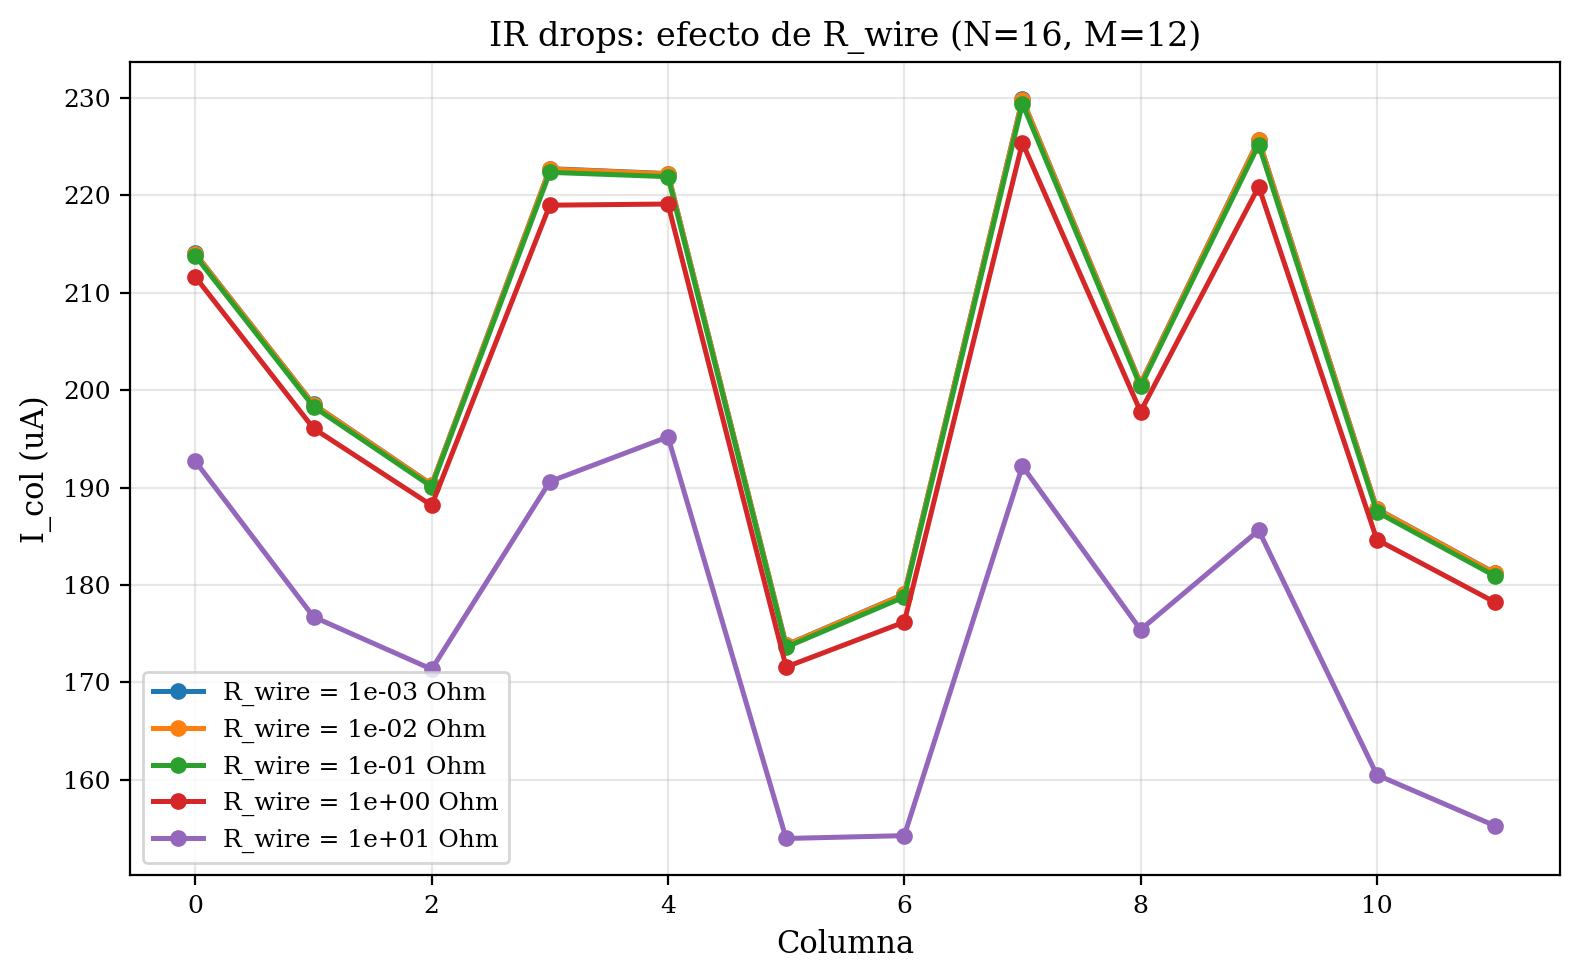
\includegraphics[width=0.72\textwidth]{experiments/figures/exp03_rwire_effect.png}
  \caption{Perfil de $I_{\text{col}}$ para distintos $R_{\text{wire}}$. La
atenuación de la corriente media aumenta con la resistencia de línea, mientras
que la dispersión entre columnas se mantiene dominada por la variabilidad de
$\mathbf{G}$.}
  \label{fig:exp03}
\end{figure}

\paragraph{Exp.~4 --- Precisión en VMM}
La Figura~\ref{fig:exp04} muestra la distribución del error relativo en VMM para 1000 vectores aleatorios. El error medio crece de $5.82\%$ ($N=4$) a $29.05\%$ ($N=24$).
\begin{figure}[H]
  \centering
  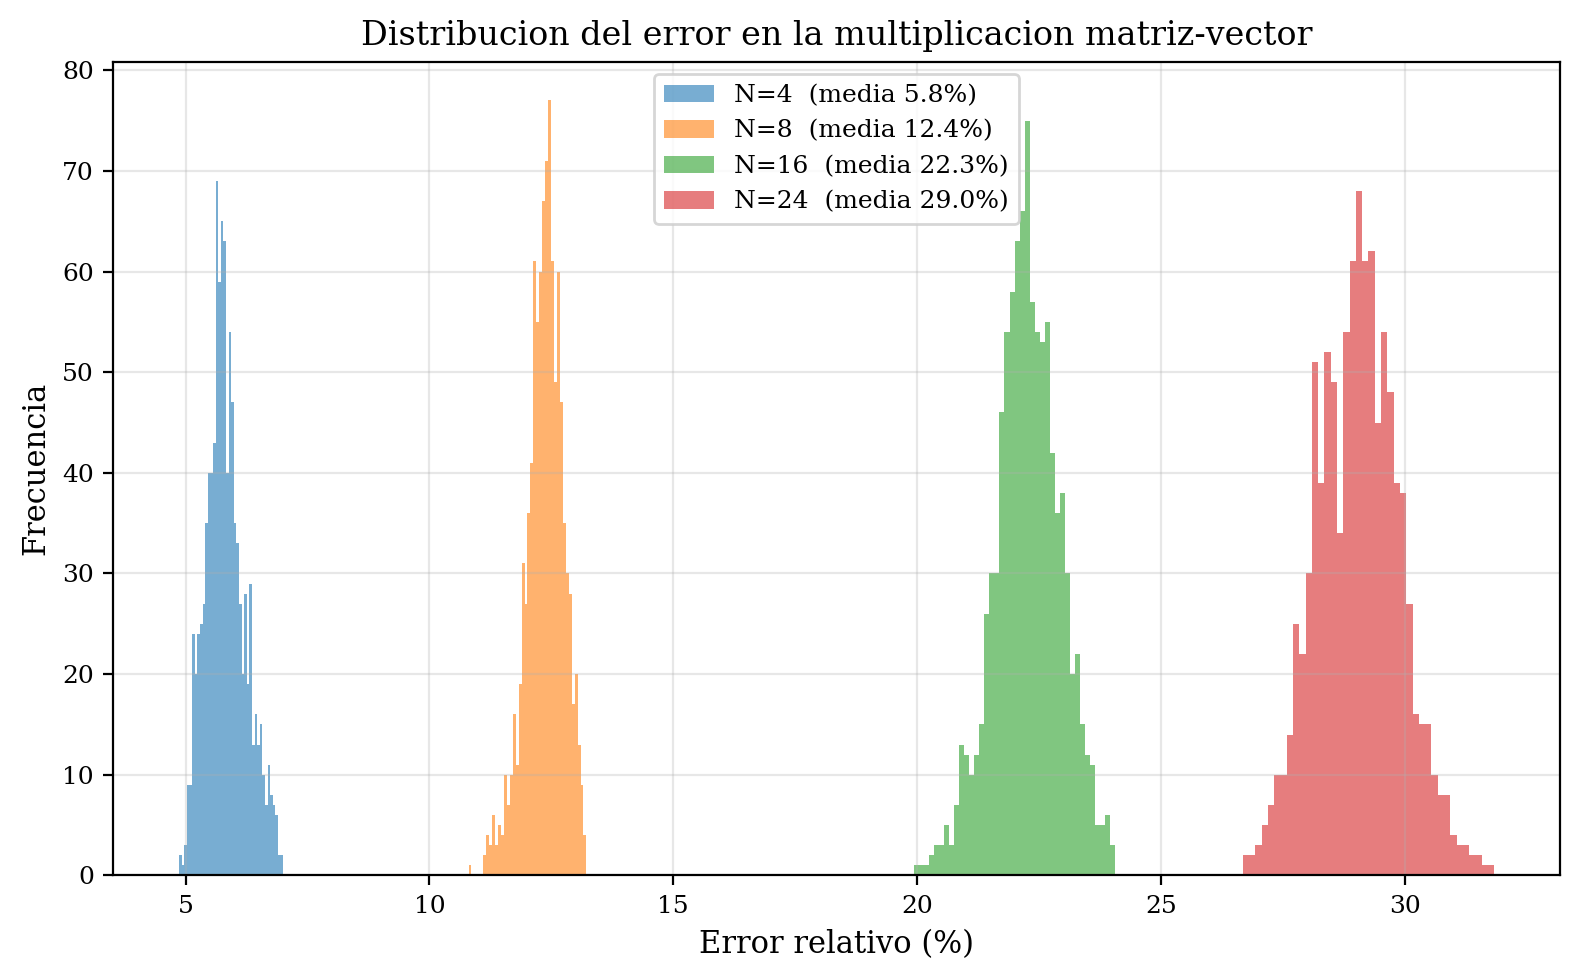
\includegraphics[width=0.70\textwidth]{experiments/figures/exp04_vmm_precision.png}
  \caption{Histograma del error relativo en VMM por tamaño de crossbar.}
  \label{fig:exp04}
\end{figure}

\paragraph{Exp.~5 --- Half-select disturb simulado: V/2 vs.\ V/3}
La Figura~\ref{fig:exp05} compara la perturbación calculada por el modelo para celdas \textit{half-selected}. Los valores reportados son 50.0\% para V/2 y 33.3\% para V/3; son razones de excitación del protocolo simulado, no medidas de disturb en celdas fabricadas.
\begin{figure}[H]
  \centering
  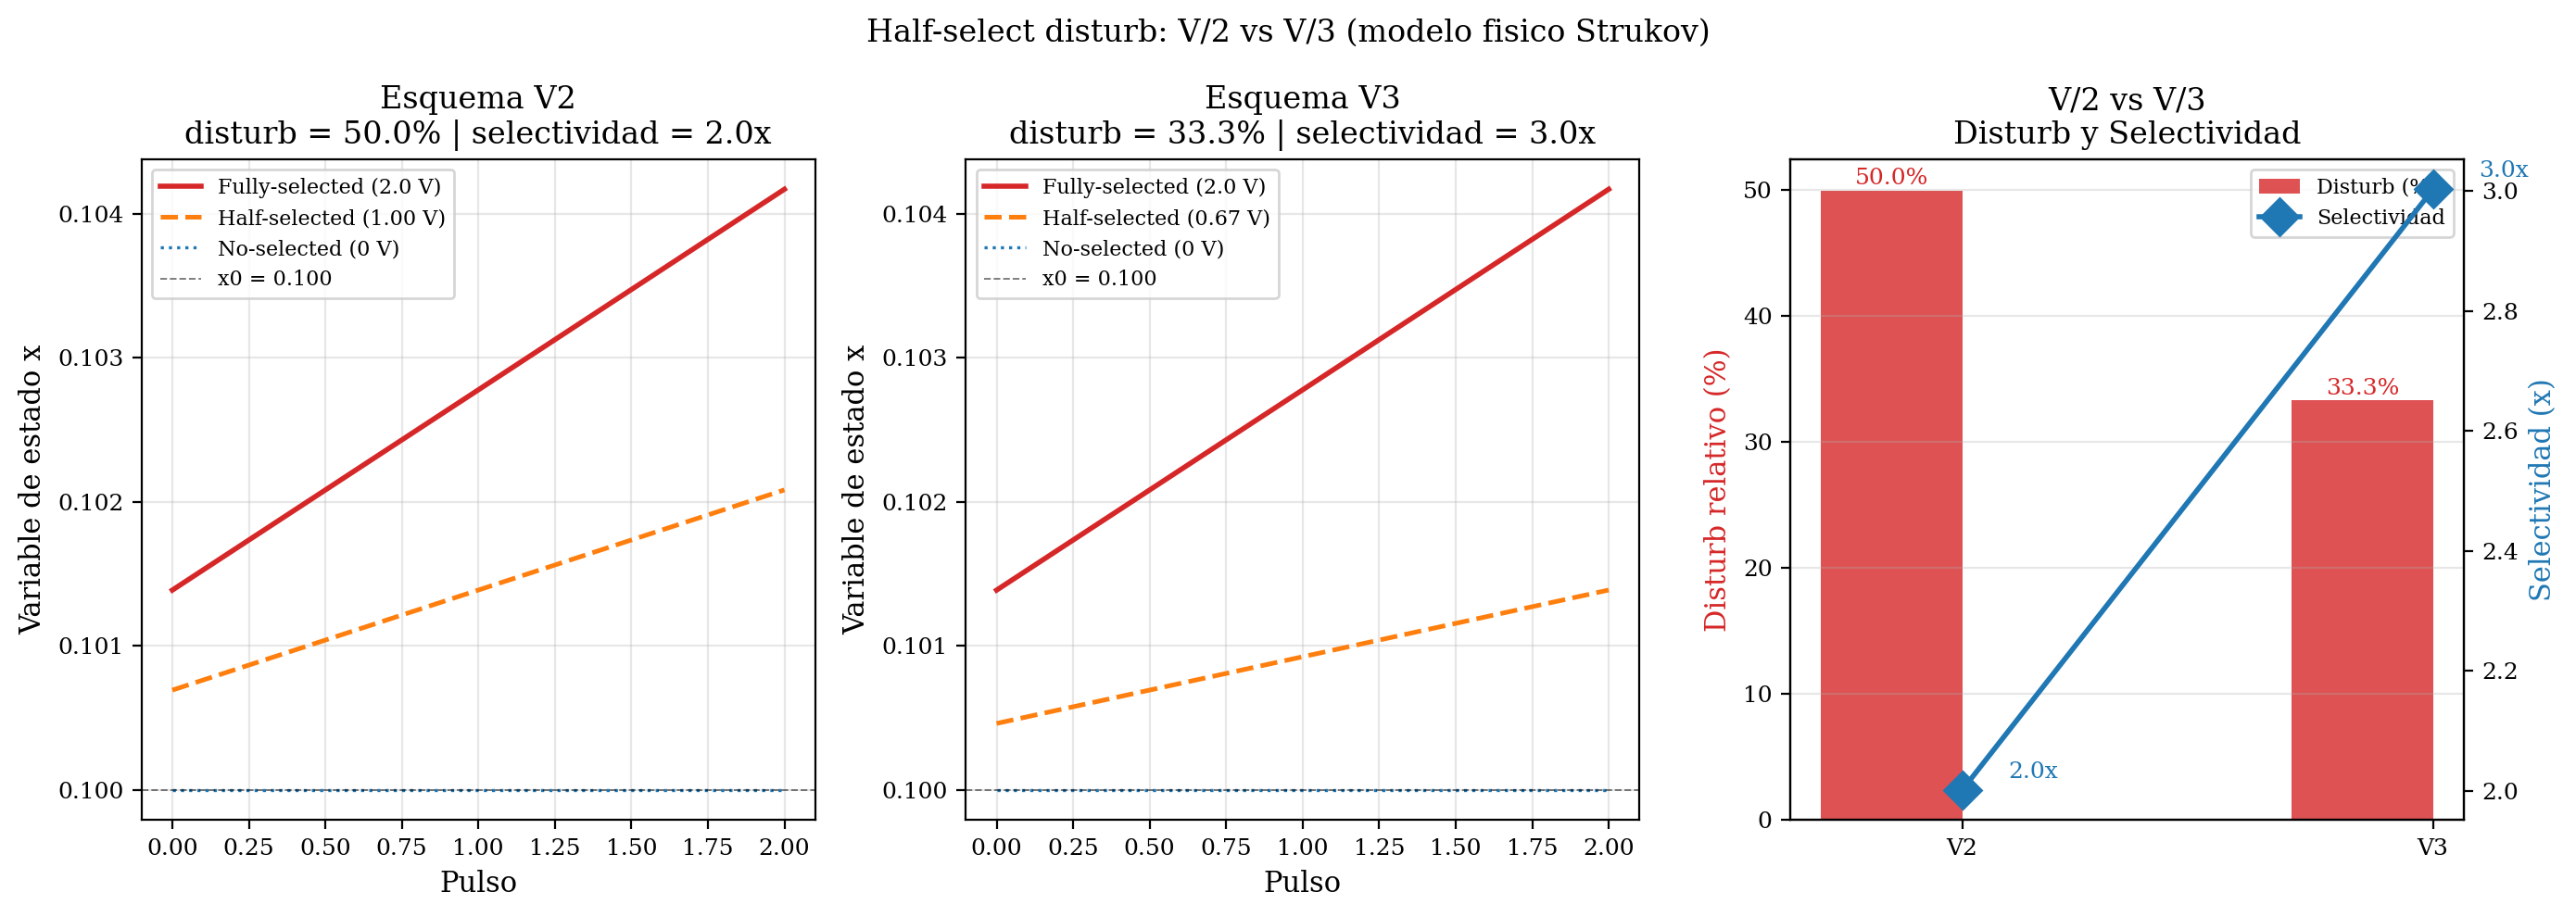
\includegraphics[width=0.95\textwidth]{experiments/figures/exp05_v2_vs_v3.png}
  \caption{Evolución de $X$ para celda fully-, half- y no-selected bajo 3 pulsos.}
  \label{fig:exp05}
\end{figure}

\paragraph{Exp.~6 --- Estado en reposo del modelo}
El resultado reportado tras 1000 pasos con $V_{\text{rows}}=0\,\text{V}$ es un cambio máximo en $X$ de $\Delta_{\max}=0$ bajo las condiciones del experimento. Esto describe el modelo y protocolo evaluados, no certifica la retención de un dispositivo físico.
\begin{figure}[H]
  \centering
  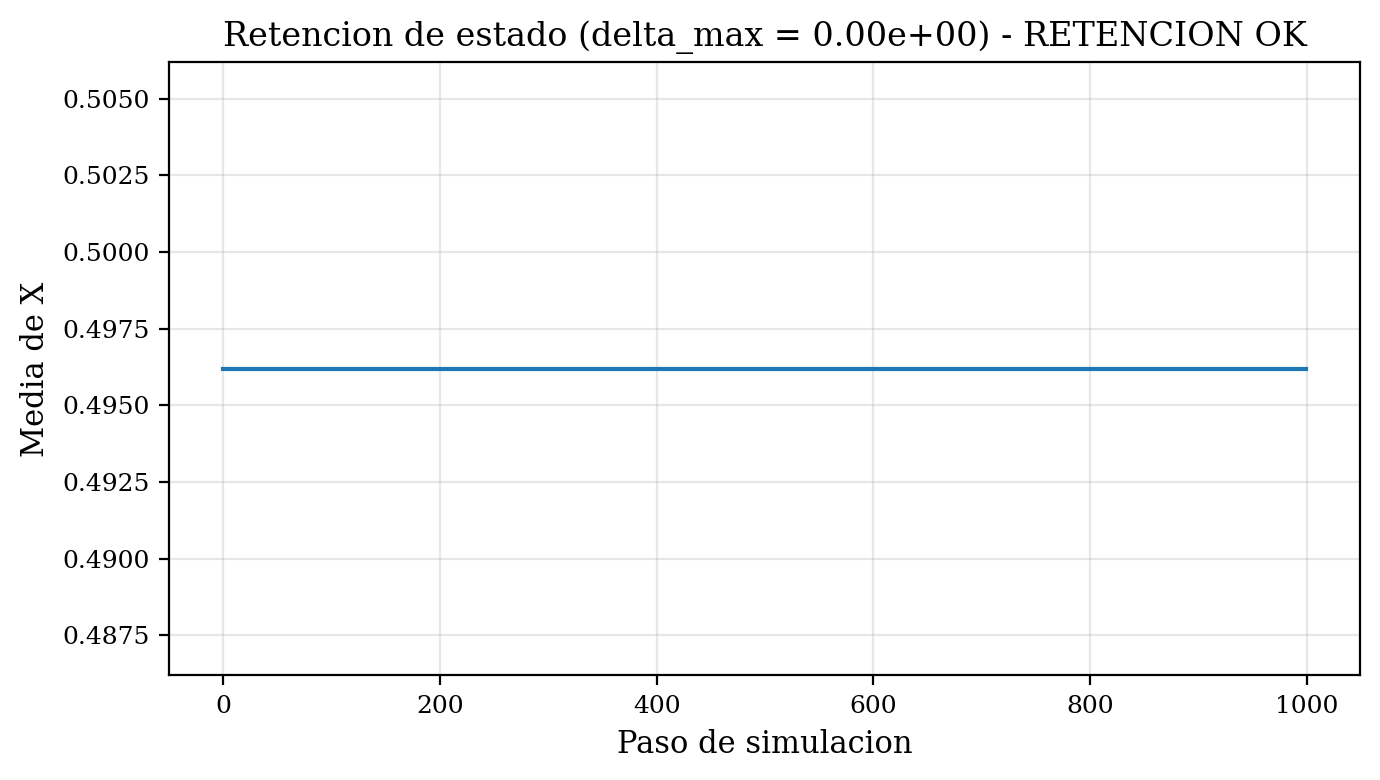
\includegraphics[width=0.62\textwidth]{experiments/figures/exp06_retention.png}
  \caption{Media de $X$ durante 1000 pasos en reposo para la simulación reportada.}
  \label{fig:exp06}
\end{figure}

\paragraph{Exp.~7 --- Respuesta simulada a pulsos LTP/LTD}
La Figura~\ref{fig:exp07} muestra la respuesta reportada del modelo bajo pulsos de potenciación (LTP, $+1\,\text{V}$) y depresión (LTD, $-1\,\text{V}$). Para 50 pulsos desde $x_0=0.1$, se reportan $x=0.135$ para LTP y $x=0.066$ para LTD. Estos valores describen la ejecución simulada y no se presentan como una respuesta experimental de un dispositivo real.
\begin{figure}[htbp]
  \centering
  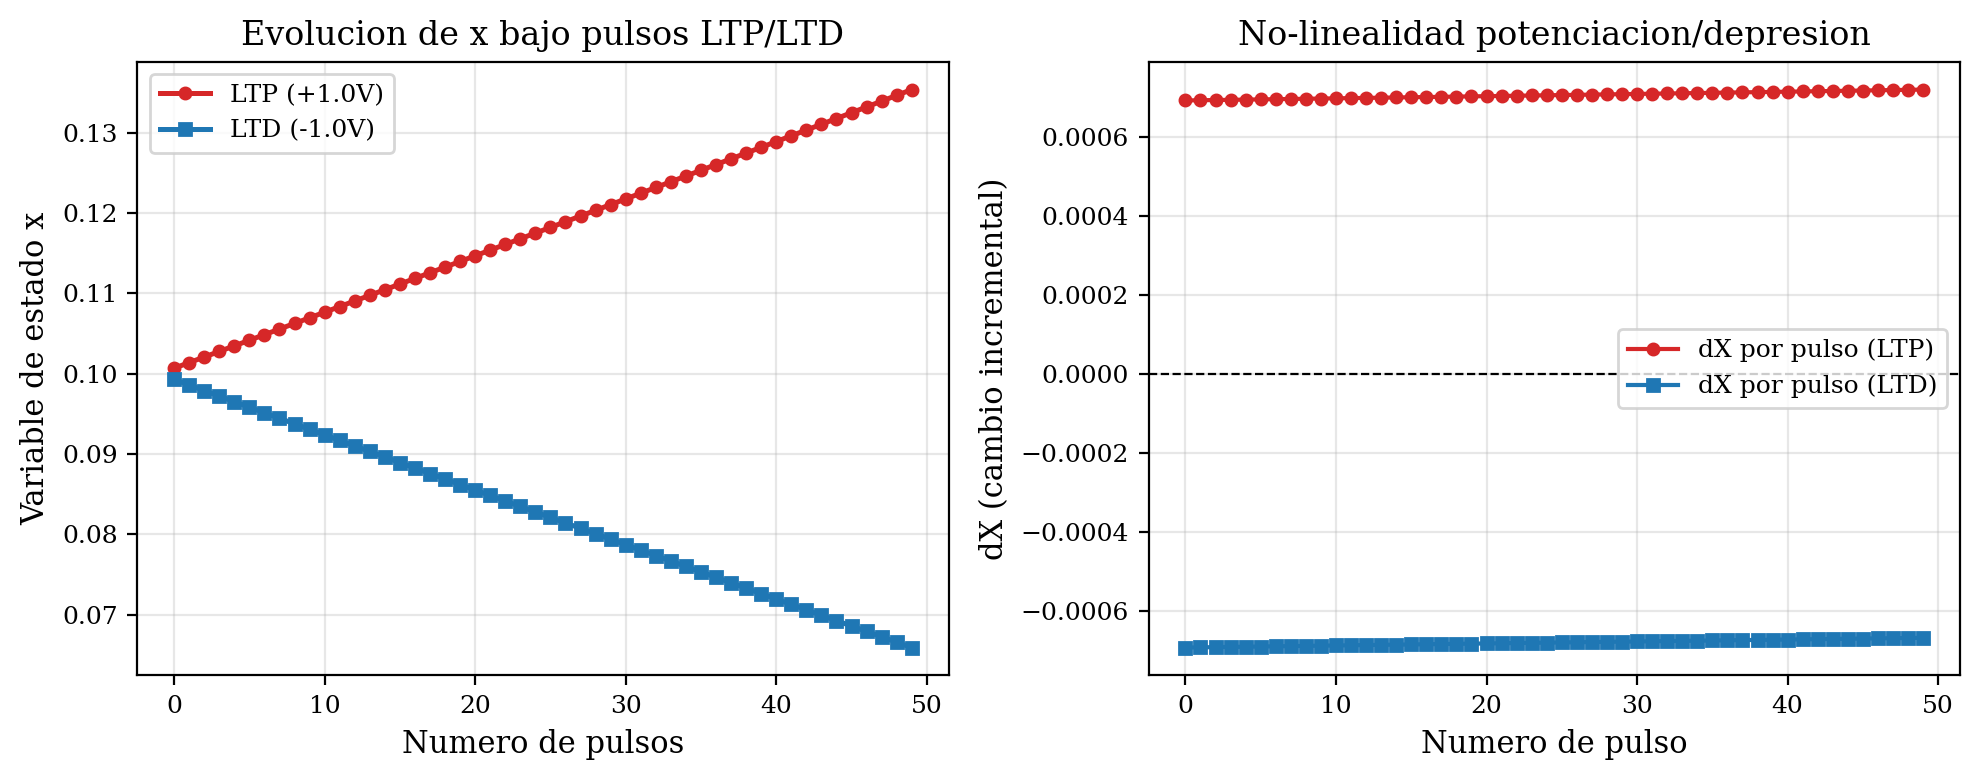
\includegraphics[width=0.88\textwidth]{experiments/figures/exp07_ltp_ltd.png}
  \caption{LTP/LTD y derivada discreta. La no-linealidad satura suavemente los extremos.}
  \label{fig:exp07}
\end{figure}

\paragraph{Exp.~8 --- Variabilidad dispositivo a dispositivo (D2D)}
La Figura~\ref{fig:exp08} cuantifica la dispersión de $I_{\text{col}}$ entre 20 crossbars virtuales. La variabilidad dispositivo-a-dispositivo se caracteriza por $CV(I_{\text{col}}) = 40.3\%$ en términos de la corriente integrada, equivalente al $4.0\%$ del rango dinámico de $\mathbf{G}$.
\begin{figure}[H]
  \centering
  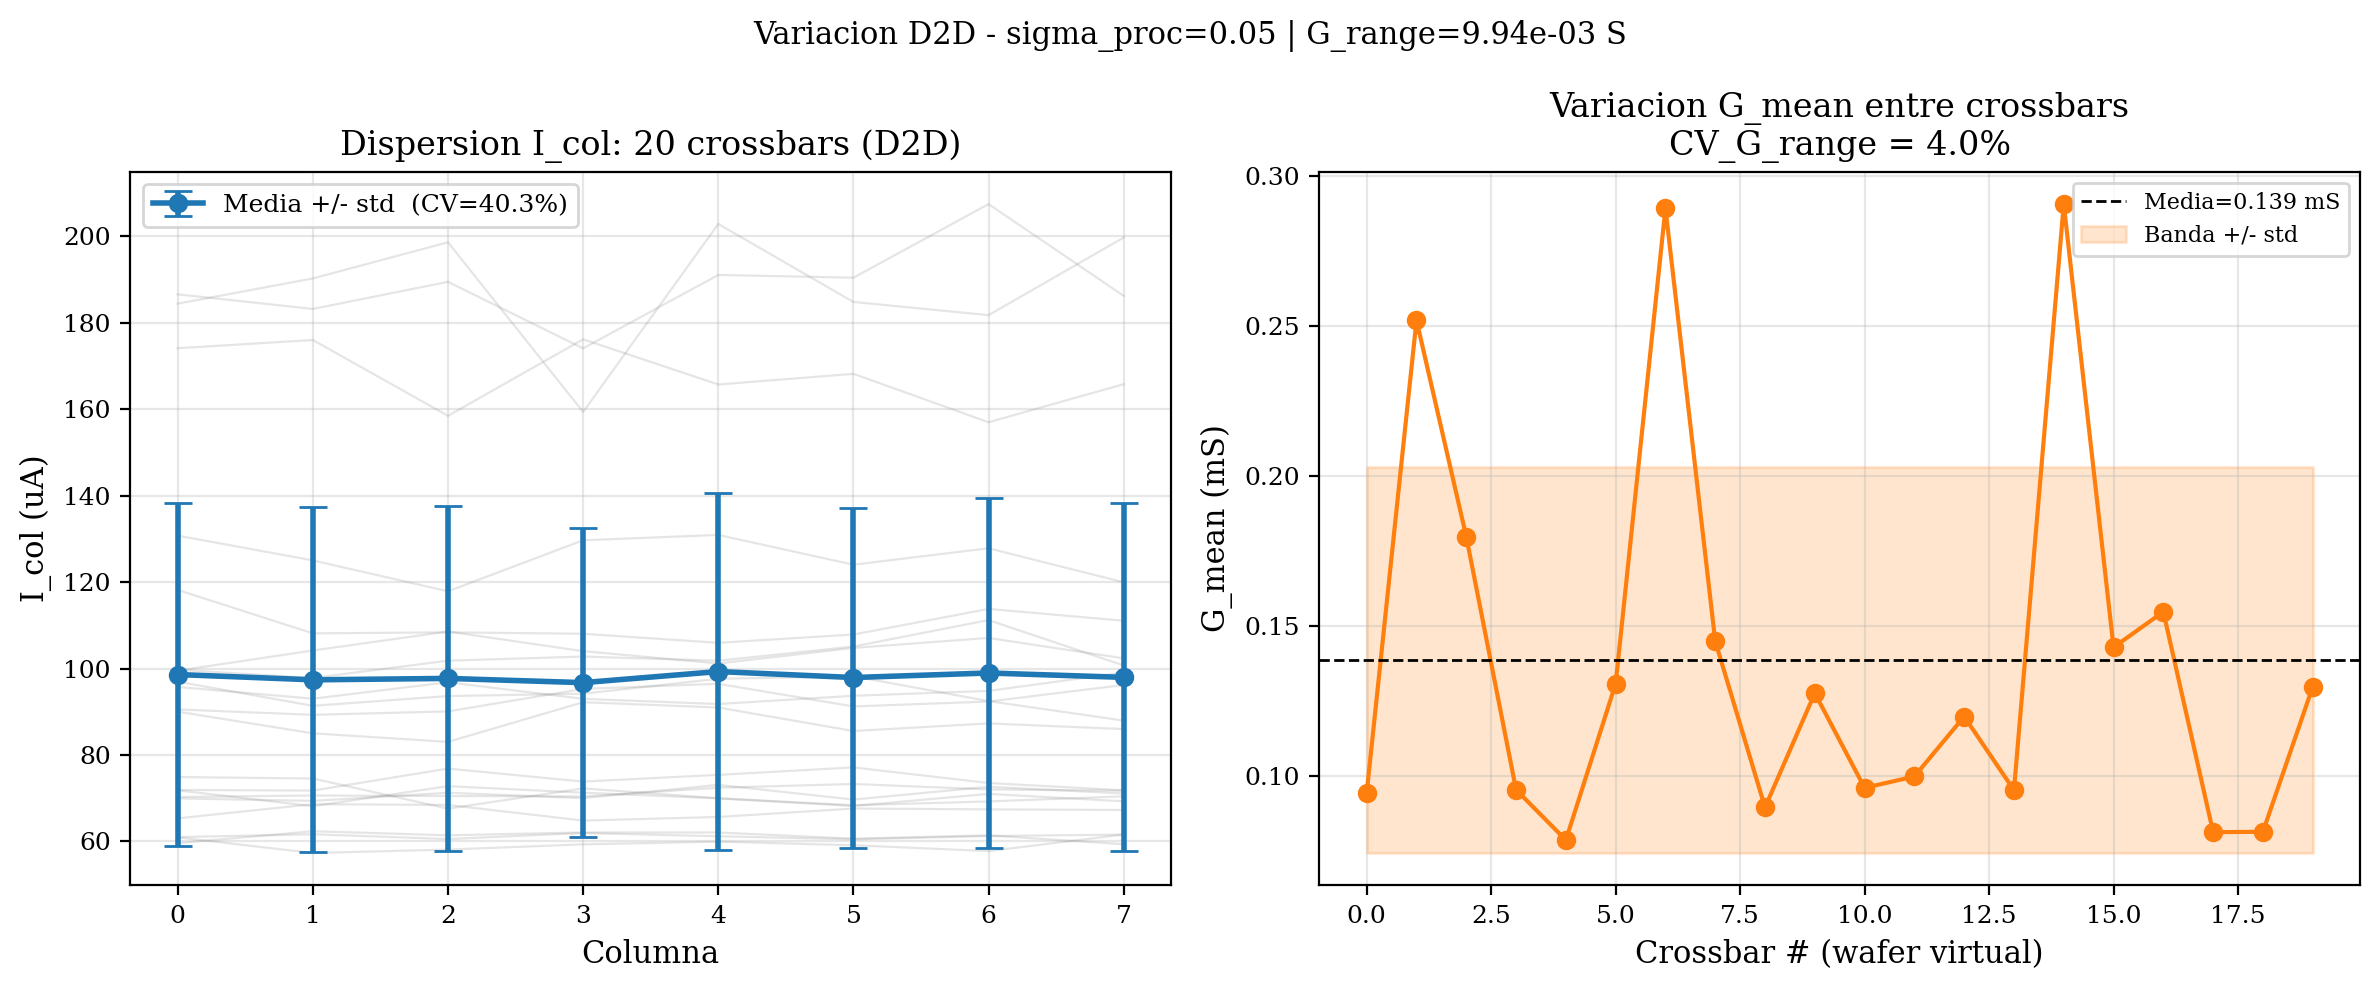
\includegraphics[width=0.88\textwidth]{experiments/figures/exp08_d2d_reproducibility.png}
  \caption{Dispersión de $I_{\text{col}}$ y variación de $\bar{G}_{\text{mean}}$ entre 20 crossbars virtuales.}
  \label{fig:exp08}
\end{figure}

\paragraph{Exp.~9 --- Costo computacional del solver MNA}
La Figura~\ref{fig:exp09} presenta un ajuste empírico reportado de
$\mathcal{O}(N^{0.85})$ y un tiempo aproximado de $\sim 3$ ms por paso para
$N=24$ en el equipo usado entonces. El exponente es propio de esa muestra y
configuración: no establece la complejidad asintótica del solver ni permite
generalizar la comparación con $\mathcal{O}(N^3)$ sin conocer el rango medido,
el hardware y el procedimiento de temporización.
\begin{figure}[H]
  \centering
  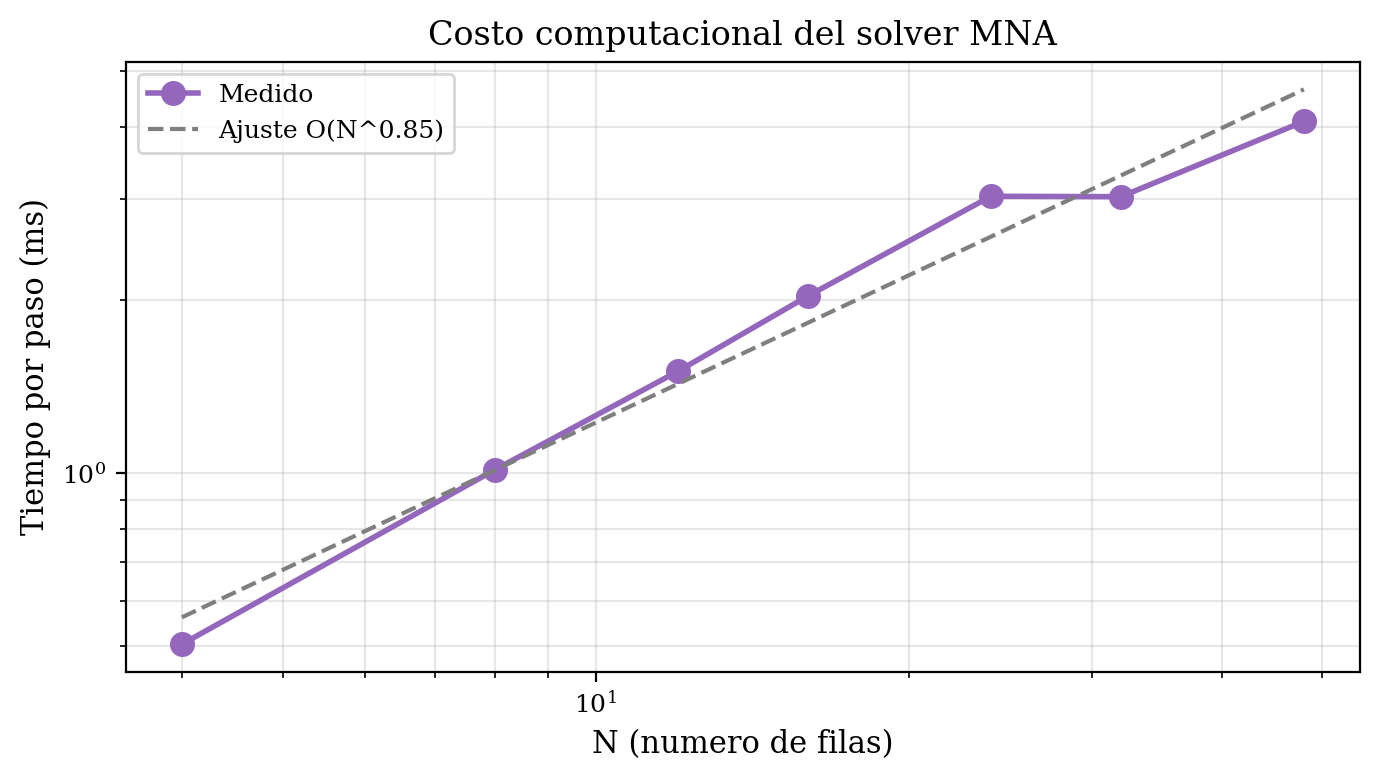
\includegraphics[width=0.62\textwidth]{experiments/figures/exp09_computational_cost.png}
  \caption{Costo computacional reportado del solver MNA en función de $N$.
El ajuste de las muestras archivadas es $\mathcal{O}(N^{0.85})$.}
  \label{fig:exp09}
\end{figure}

\paragraph{Exp.~10 --- Crosstalk entre columnas}
La Figura~\ref{fig:exp10} expone el efecto de crosstalk: al excitar únicamente la fila 0, las otras columnas muestran una desviación media del $13.32\%$ por interacción parásita MNA.
\begin{figure}[H]
  \centering
  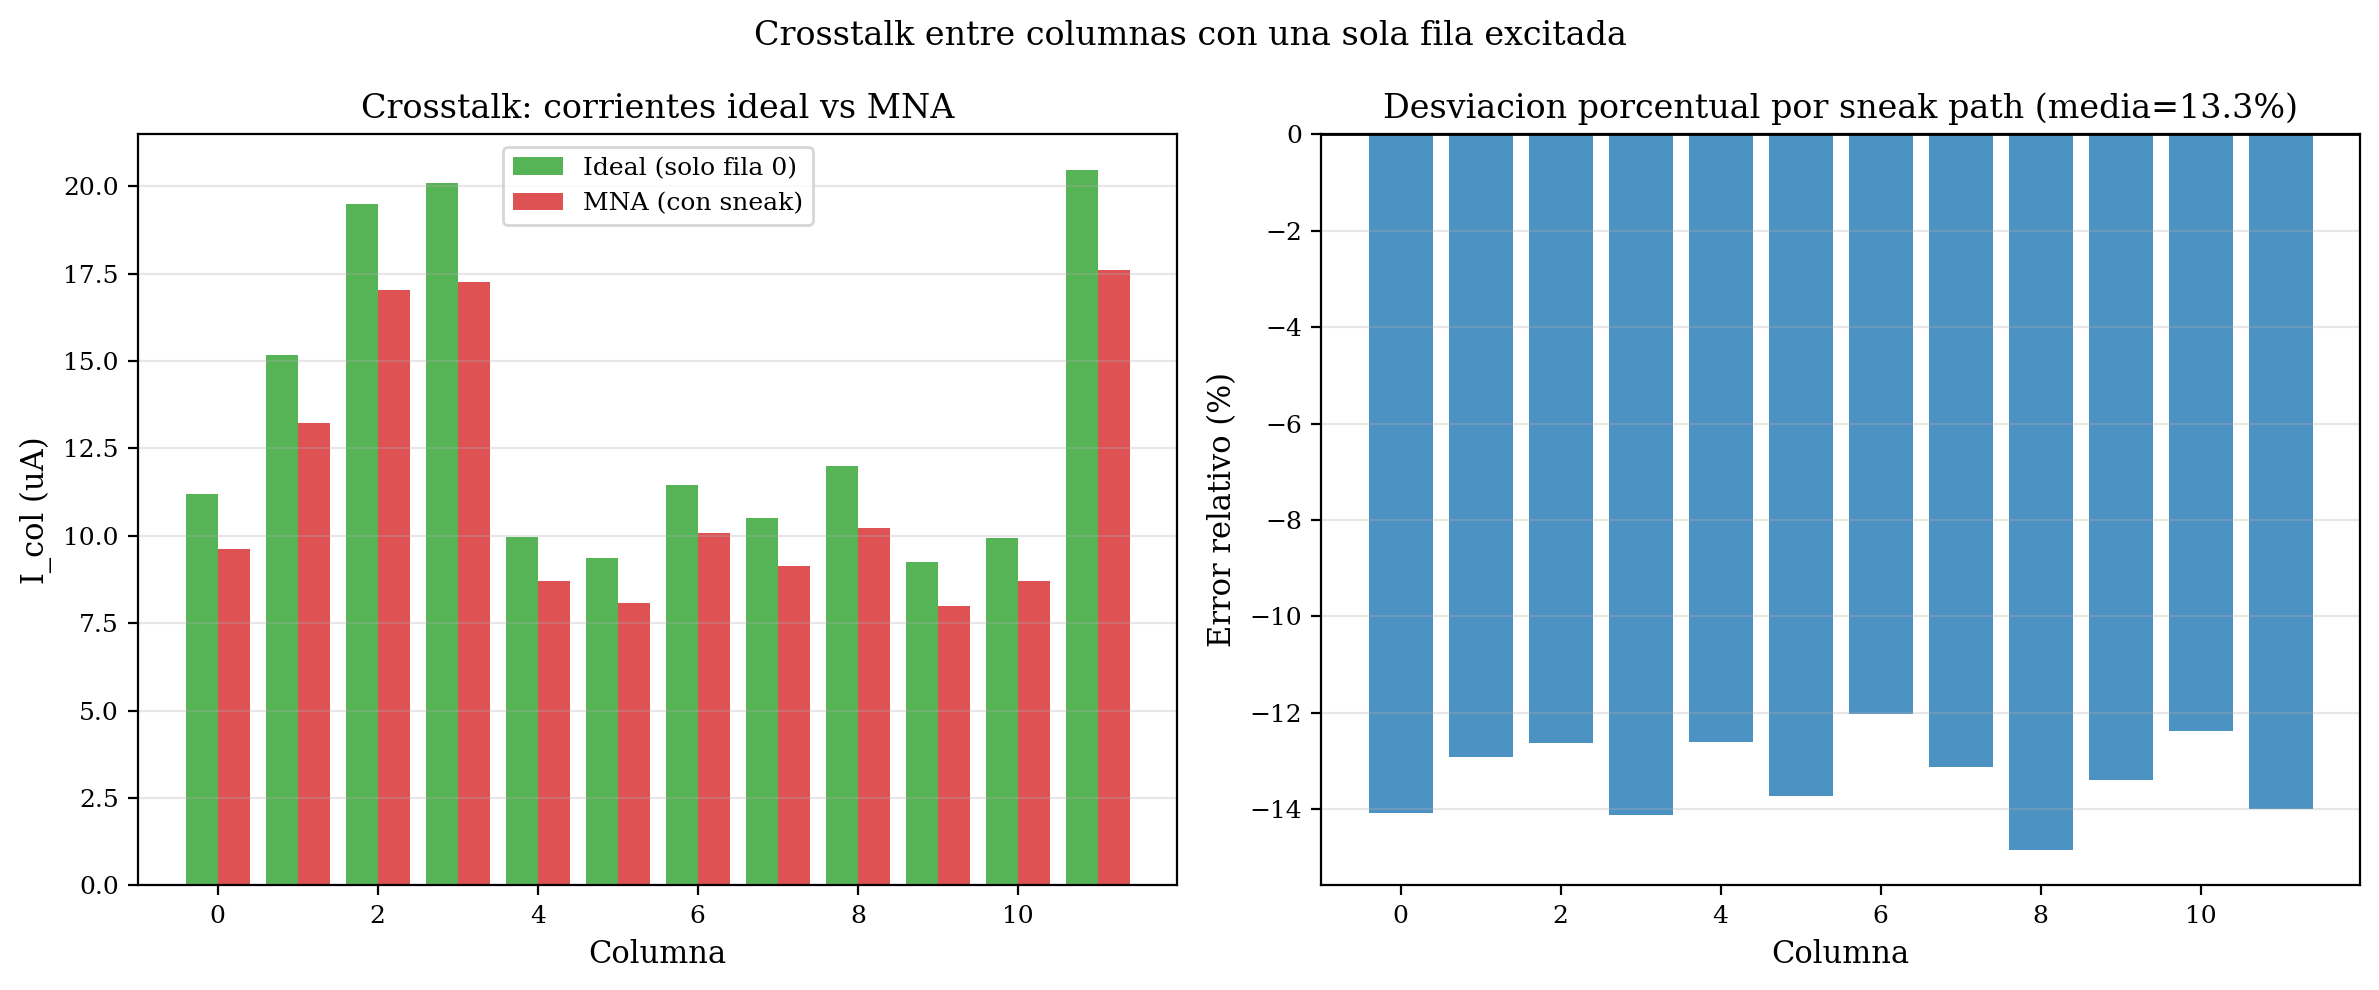
\includegraphics[width=0.88\textwidth]{experiments/figures/exp10_crosstalk.png}
  \caption{$I_{\text{col}}$ real vs.\ ideal al excitar únicamente la fila 0.}
  \label{fig:exp10}
\end{figure}

\paragraph{Alcance de los resultados de la Etapa 4}
Los diez experimentos anteriores y las figuras del agente documentan
resultados guardados de simulaciones, no mediciones de hardware. Para evitar
repetir sus cifras en un segundo resumen, esta sección deja cada resultado
junto a su configuración y figura; la tabla maestra del Apéndice C resume
únicamente las verificaciones V01--V28.



% Figuras originales de los registros de entrenamiento archivados.
\chapter{Evidencia visual de los entrenamientos}
\label{ap:evidencia_entrenamientos}

Este ap\'endice re\'une las figuras ya generadas y archivadas para las condiciones de entrenamiento seleccionadas. Cada condici\'on muestra el estado final del crossbar y la curva de \'exito de su propio registro; las figuras no son corridas adicionales. El primer lote contiene 28 condiciones (CartPole, visi\'on, obst\'aculos y Car R-STDP; semillas 0 y 1; $X_0=0.1$ y $X_0=0.9$). El segundo contiene cuatro condiciones adicionales de Car R-STDP (semillas 2 y 4), con evaluaci\'on cada 100 episodios. Los protocolos, registros JSON, matrices y hashes est\'an en las carpetas citadas en cada bloque.

La curva corresponde a la tasa de \'exito durante el entrenamiento. El campo de criterio indica si el registro cumpli\'o la regla de parada de su protocolo; la evaluaci\'on greedy y la evaluaci\'on en mapas apartados, cuando existen, se informan por separado en las tablas de resultados. El umbral de ventana m\'ovil es 271 \'exitos de 300 episodios (90.33\%), no 300 \'exitos consecutivos.
\clearpage

\noindent\textbf{CartPole | REINFORCE | semilla 0 | $X_0=0.1$}\\
{\scriptsize lote principal; episodios completados: 349; tasa de \'exito en la ventana final: 90.33\%; criterio alcanzado: s\'i.}\par
\noindent\begin{minipage}[t]{0.49\textwidth}
\centering
\textit{Crossbar $X$}\par
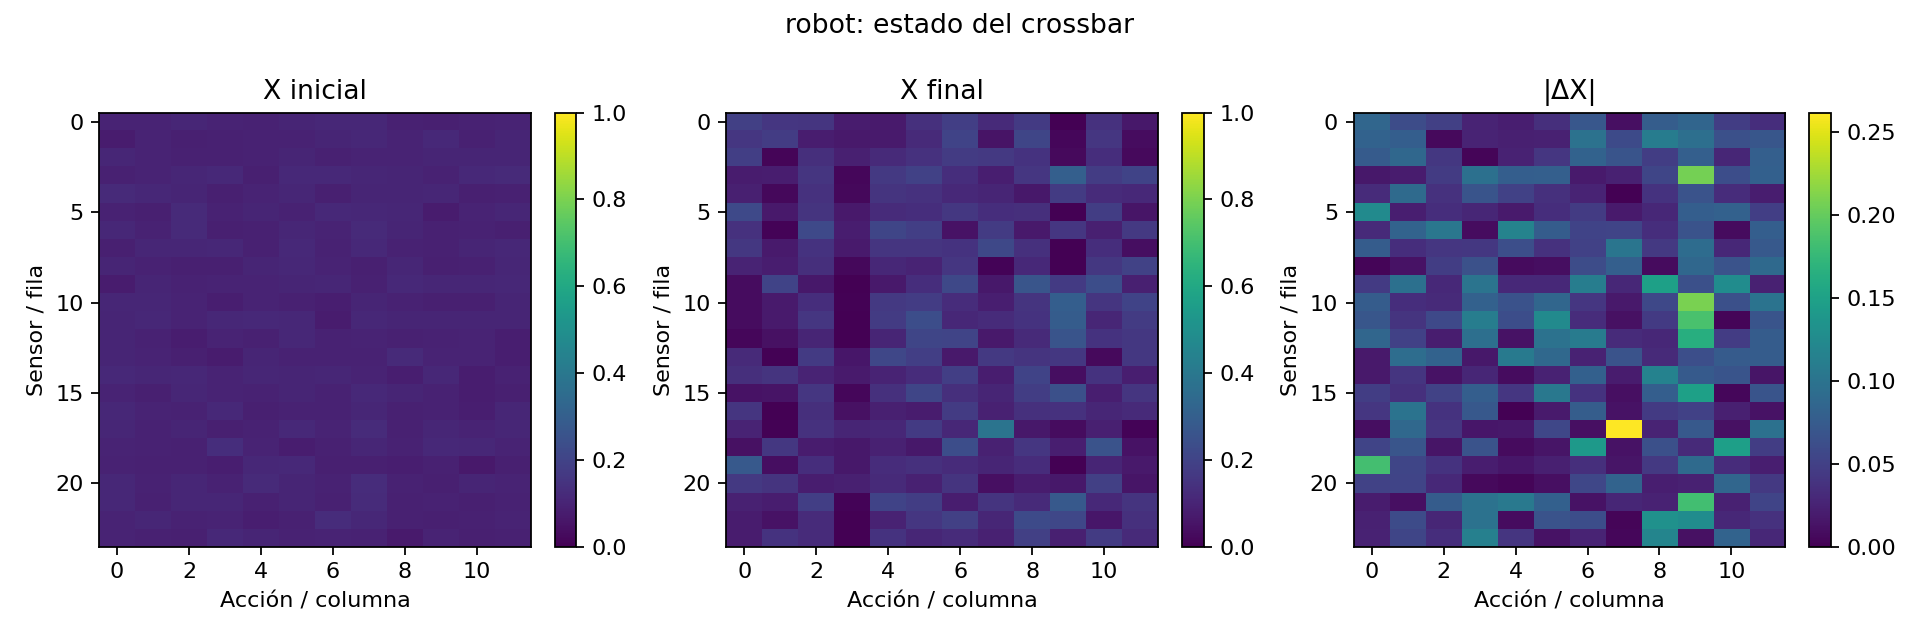
\includegraphics[width=\linewidth,height=0.14\textheight,keepaspectratio]{../../03_EVIDENCIAS/ENTRENAMIENTOS/COMPARATIVA_SEEDS_0_1_X0/runs/robot_reinforce_seed0_X0_0.1/crossbar.png}
\end{minipage}\hfill
\begin{minipage}[t]{0.49\textwidth}
\centering
\textit{Curva de \'exito}\par
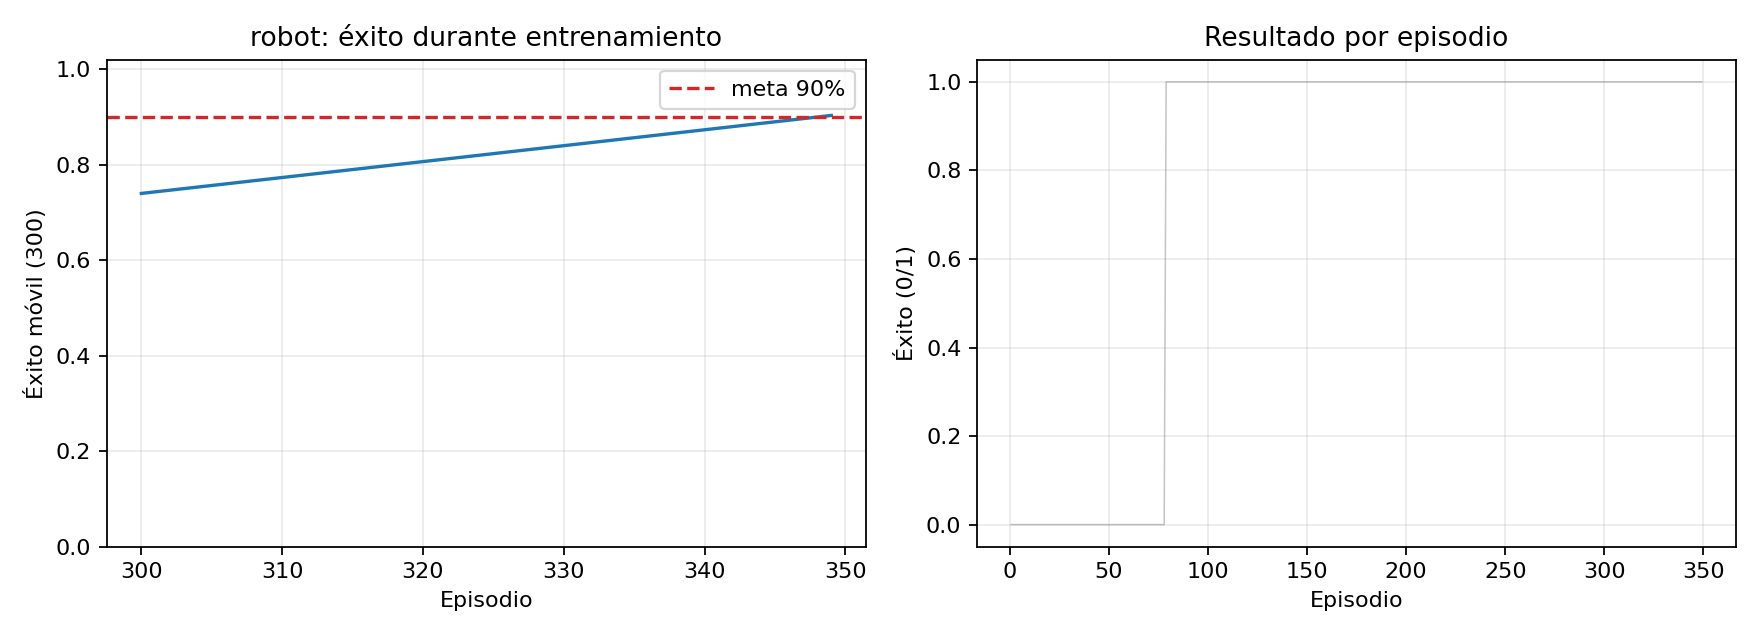
\includegraphics[width=\linewidth,height=0.14\textheight,keepaspectratio]{../../03_EVIDENCIAS/ENTRENAMIENTOS/COMPARATIVA_SEEDS_0_1_X0/runs/robot_reinforce_seed0_X0_0.1/success_curve.png}
\end{minipage}\par\smallskip
\noindent\textbf{CartPole | REINFORCE | semilla 0 | $X_0=0.9$}\\
{\scriptsize lote principal; episodios completados: 559; tasa de \'exito en la ventana final: 0.00\%; criterio alcanzado: no.}\par
\noindent\begin{minipage}[t]{0.49\textwidth}
\centering
\textit{Crossbar $X$}\par
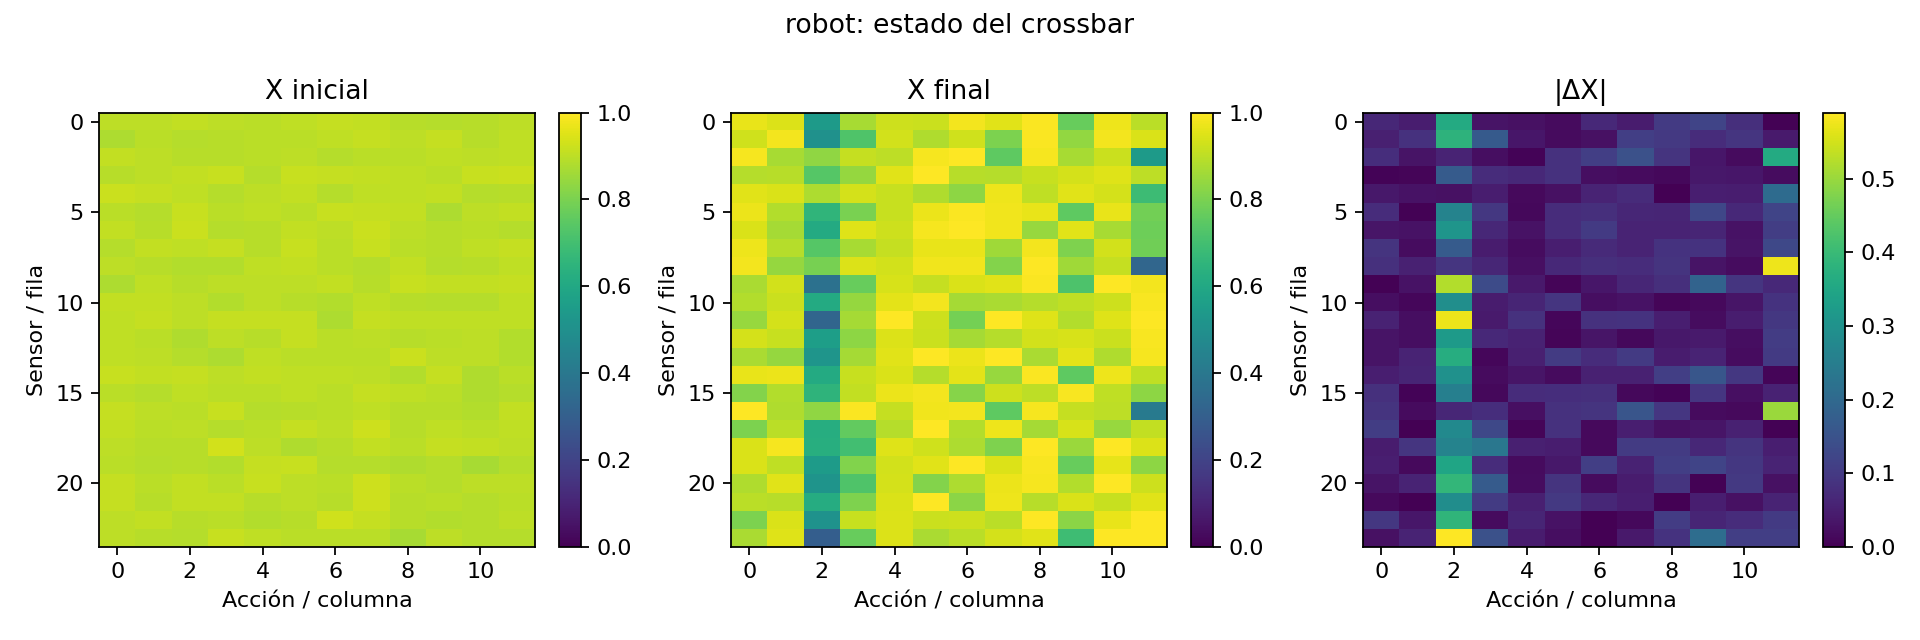
\includegraphics[width=\linewidth,height=0.14\textheight,keepaspectratio]{../../03_EVIDENCIAS/ENTRENAMIENTOS/COMPARATIVA_SEEDS_0_1_X0/runs/robot_reinforce_seed0_X0_0.9/crossbar.png}
\end{minipage}\hfill
\begin{minipage}[t]{0.49\textwidth}
\centering
\textit{Curva de \'exito}\par
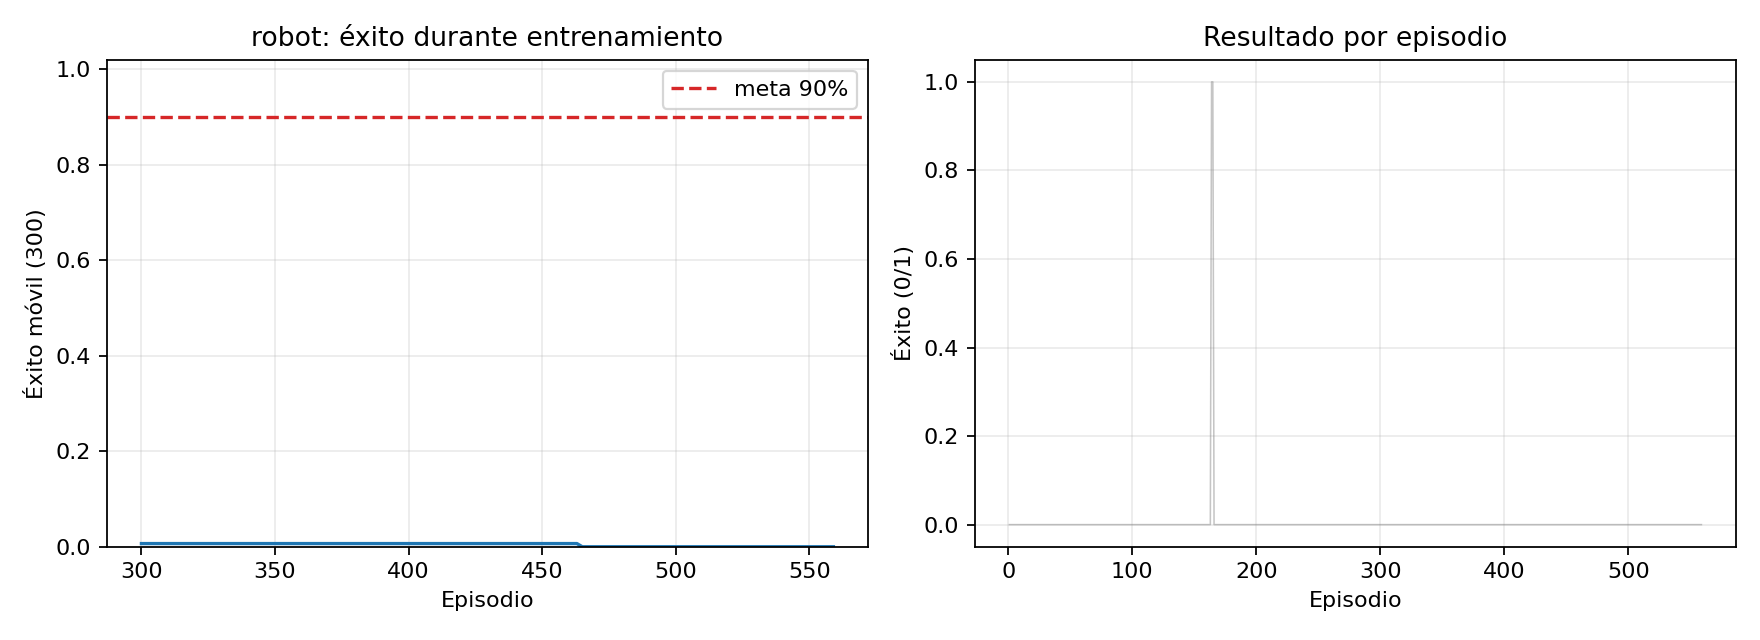
\includegraphics[width=\linewidth,height=0.14\textheight,keepaspectratio]{../../03_EVIDENCIAS/ENTRENAMIENTOS/COMPARATIVA_SEEDS_0_1_X0/runs/robot_reinforce_seed0_X0_0.9/success_curve.png}
\end{minipage}\par\smallskip
\noindent\textbf{CartPole | REINFORCE | semilla 1 | $X_0=0.1$}\\
{\scriptsize lote principal; episodios completados: 1132; tasa de \'exito en la ventana final: 0.00\%; criterio alcanzado: no.}\par
\noindent\begin{minipage}[t]{0.49\textwidth}
\centering
\textit{Crossbar $X$}\par
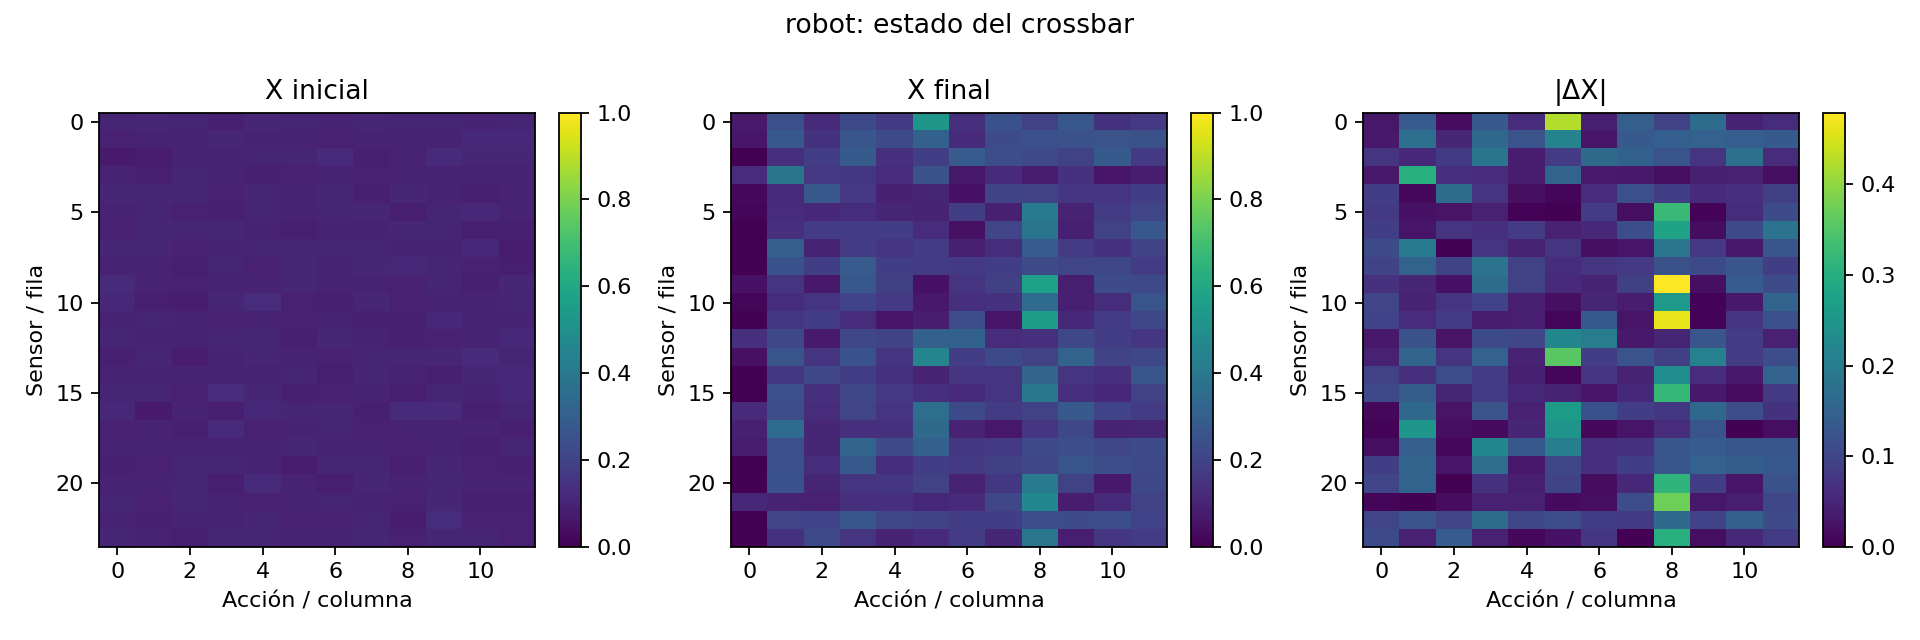
\includegraphics[width=\linewidth,height=0.14\textheight,keepaspectratio]{../../03_EVIDENCIAS/ENTRENAMIENTOS/COMPARATIVA_SEEDS_0_1_X0/runs/robot_reinforce_seed1_X0_0.1/crossbar.png}
\end{minipage}\hfill
\begin{minipage}[t]{0.49\textwidth}
\centering
\textit{Curva de \'exito}\par
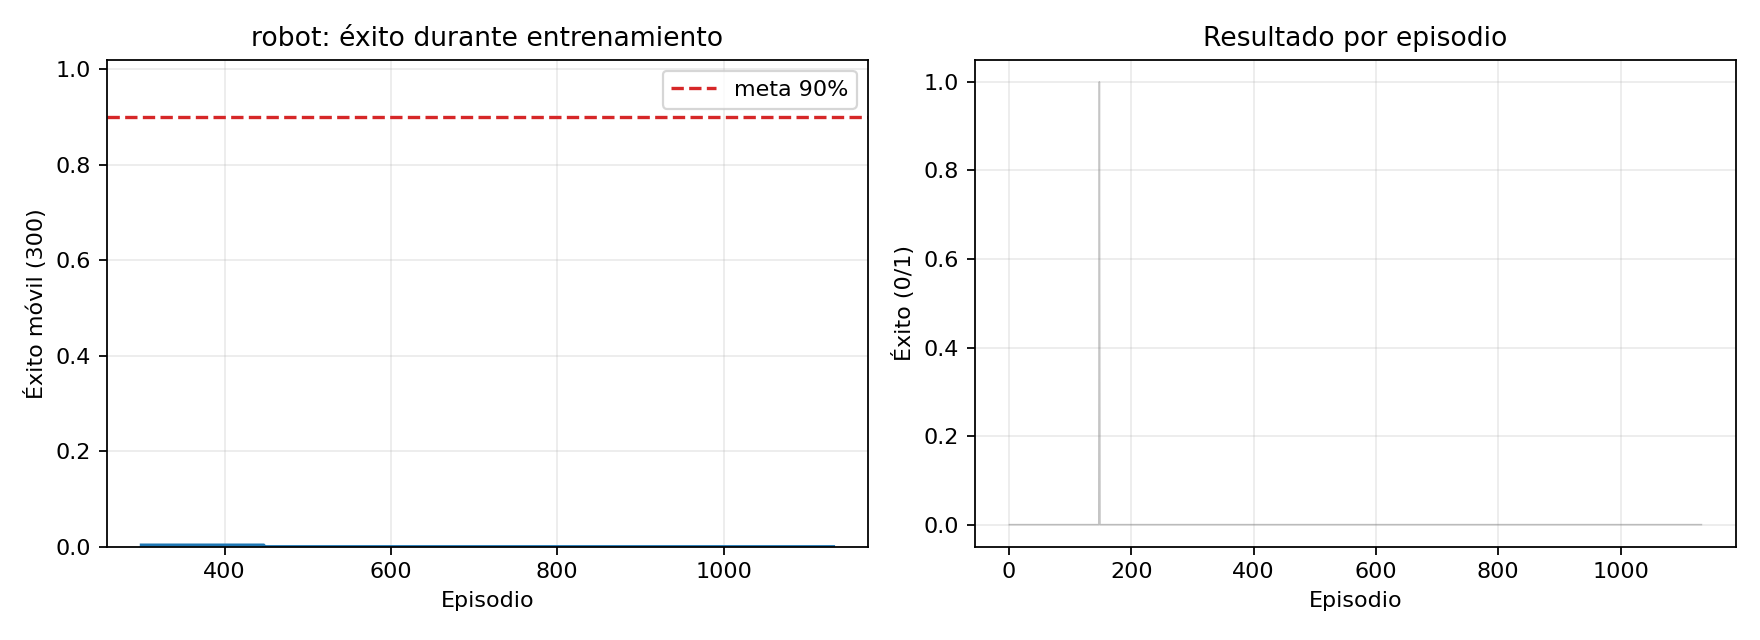
\includegraphics[width=\linewidth,height=0.14\textheight,keepaspectratio]{../../03_EVIDENCIAS/ENTRENAMIENTOS/COMPARATIVA_SEEDS_0_1_X0/runs/robot_reinforce_seed1_X0_0.1/success_curve.png}
\end{minipage}\par\smallskip
\noindent\textbf{CartPole | REINFORCE | semilla 1 | $X_0=0.9$}\\
{\scriptsize lote principal; episodios completados: 1249; tasa de \'exito en la ventana final: 90.33\%; criterio alcanzado: s\'i.}\par
\noindent\begin{minipage}[t]{0.49\textwidth}
\centering
\textit{Crossbar $X$}\par
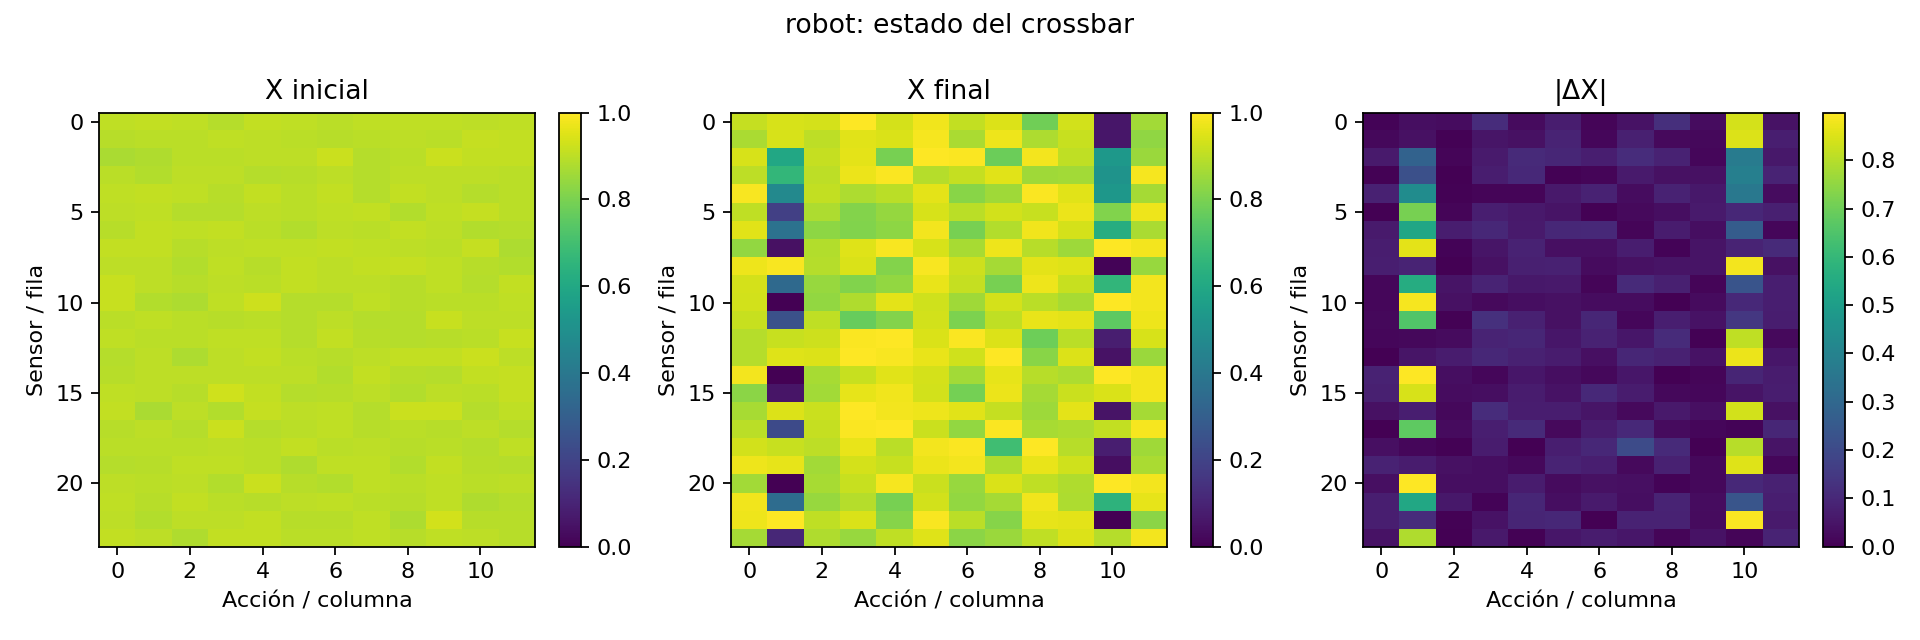
\includegraphics[width=\linewidth,height=0.14\textheight,keepaspectratio]{../../03_EVIDENCIAS/ENTRENAMIENTOS/COMPARATIVA_SEEDS_0_1_X0/runs/robot_reinforce_seed1_X0_0.9/crossbar.png}
\end{minipage}\hfill
\begin{minipage}[t]{0.49\textwidth}
\centering
\textit{Curva de \'exito}\par
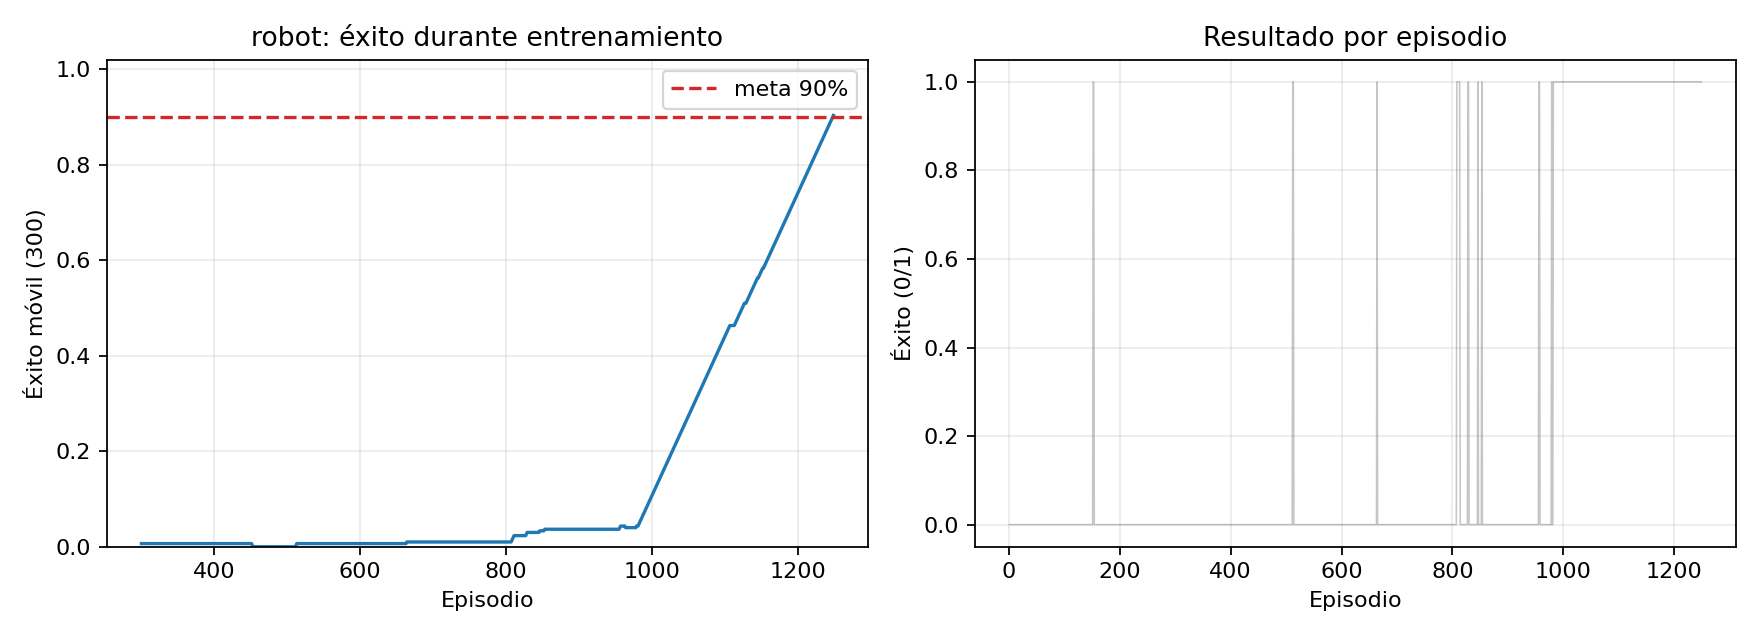
\includegraphics[width=\linewidth,height=0.14\textheight,keepaspectratio]{../../03_EVIDENCIAS/ENTRENAMIENTOS/COMPARATIVA_SEEDS_0_1_X0/runs/robot_reinforce_seed1_X0_0.9/success_curve.png}
\end{minipage}\par\smallskip
\clearpage
\noindent\textbf{CartPole | R-STDP | semilla 0 | $X_0=0.1$}\\
{\scriptsize lote principal; episodios completados: 307; tasa de \'exito en la ventana final: 90.33\%; criterio alcanzado: s\'i.}\par
\noindent\begin{minipage}[t]{0.49\textwidth}
\centering
\textit{Crossbar $X$}\par
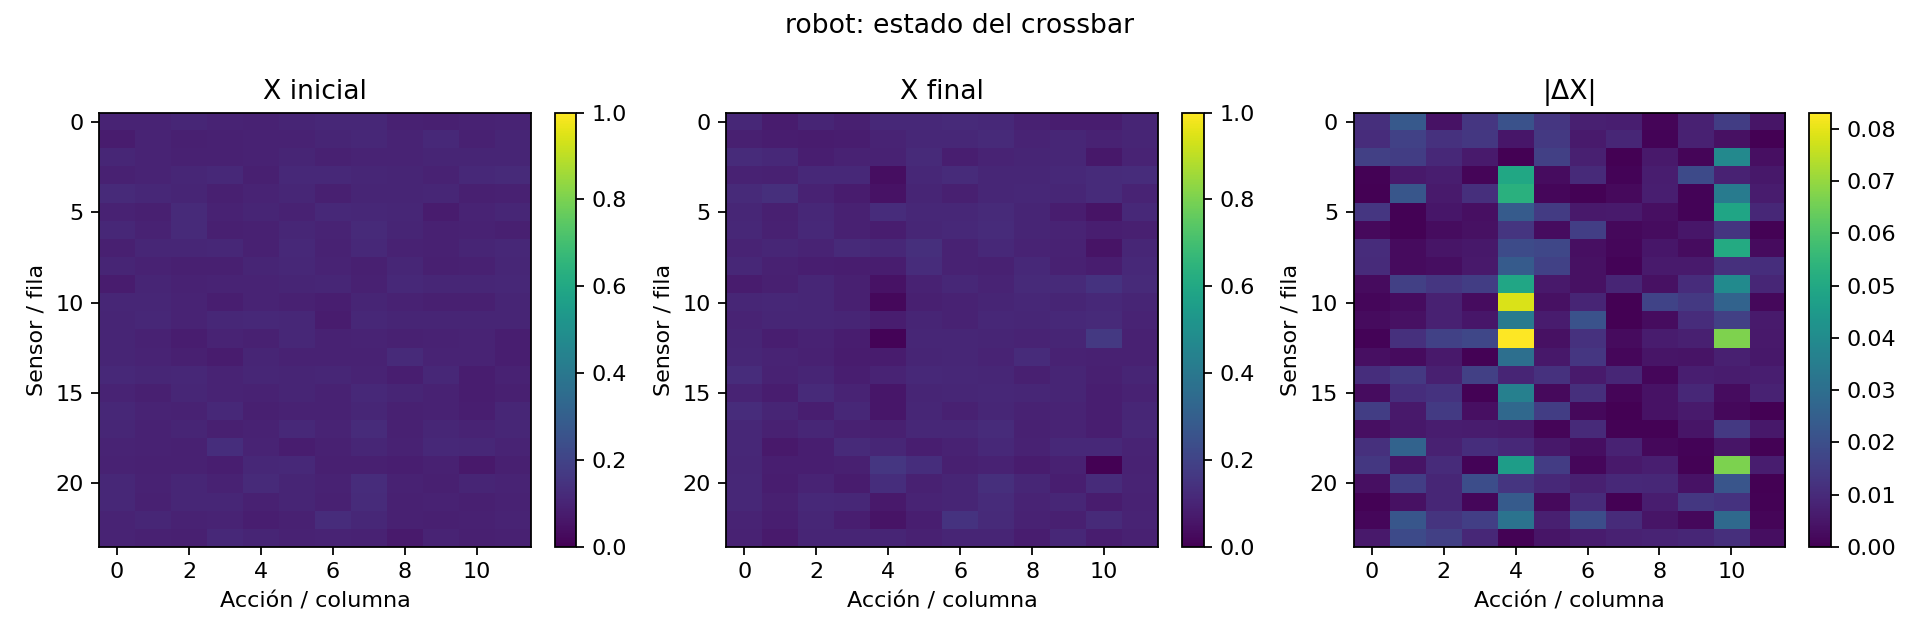
\includegraphics[width=\linewidth,height=0.14\textheight,keepaspectratio]{../../03_EVIDENCIAS/ENTRENAMIENTOS/COMPARATIVA_SEEDS_0_1_X0/runs/robot_rstdp_seed0_X0_0.1/crossbar.png}
\end{minipage}\hfill
\begin{minipage}[t]{0.49\textwidth}
\centering
\textit{Curva de \'exito}\par
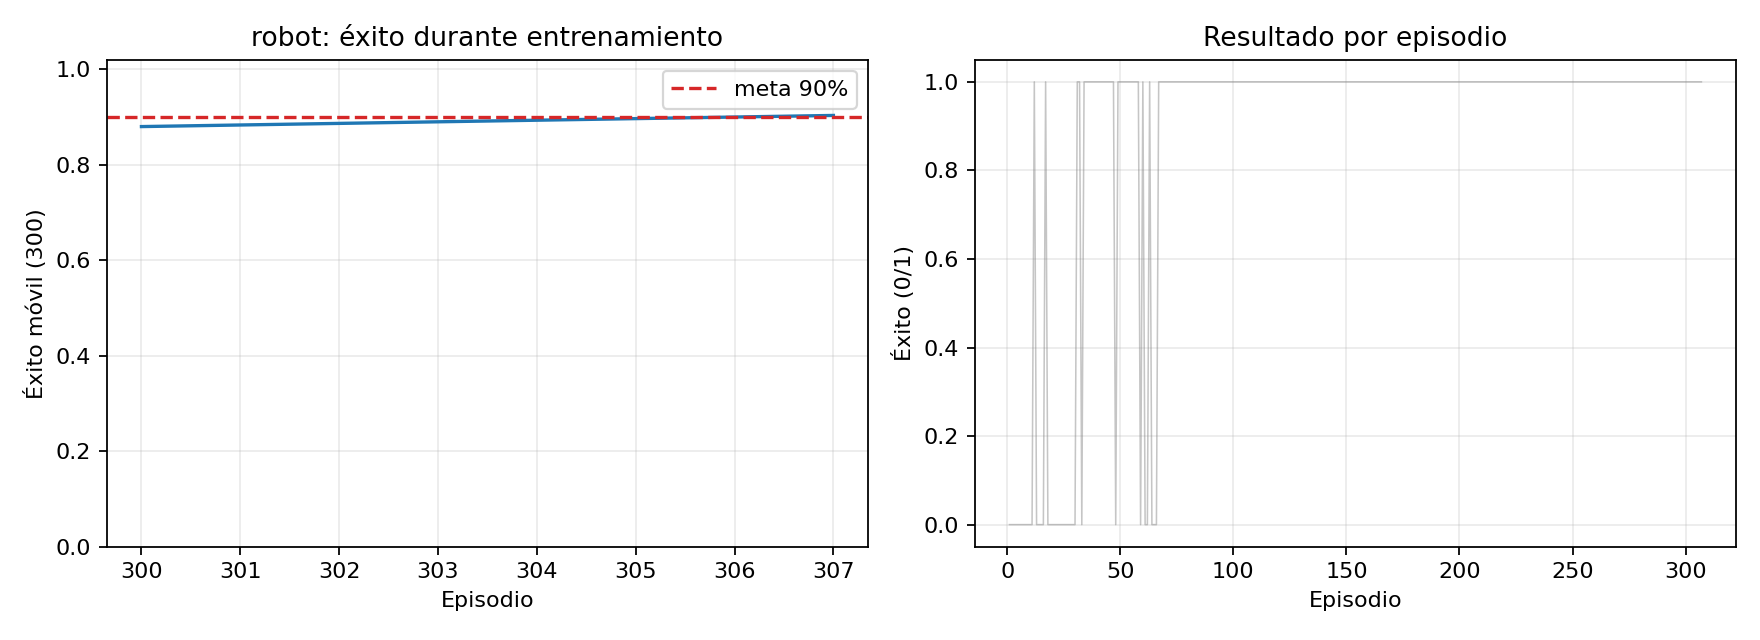
\includegraphics[width=\linewidth,height=0.14\textheight,keepaspectratio]{../../03_EVIDENCIAS/ENTRENAMIENTOS/COMPARATIVA_SEEDS_0_1_X0/runs/robot_rstdp_seed0_X0_0.1/success_curve.png}
\end{minipage}\par\smallskip
\noindent\textbf{CartPole | R-STDP | semilla 0 | $X_0=0.9$}\\
{\scriptsize lote principal; episodios completados: 393; tasa de \'exito en la ventana final: 90.33\%; criterio alcanzado: s\'i.}\par
\noindent\begin{minipage}[t]{0.49\textwidth}
\centering
\textit{Crossbar $X$}\par
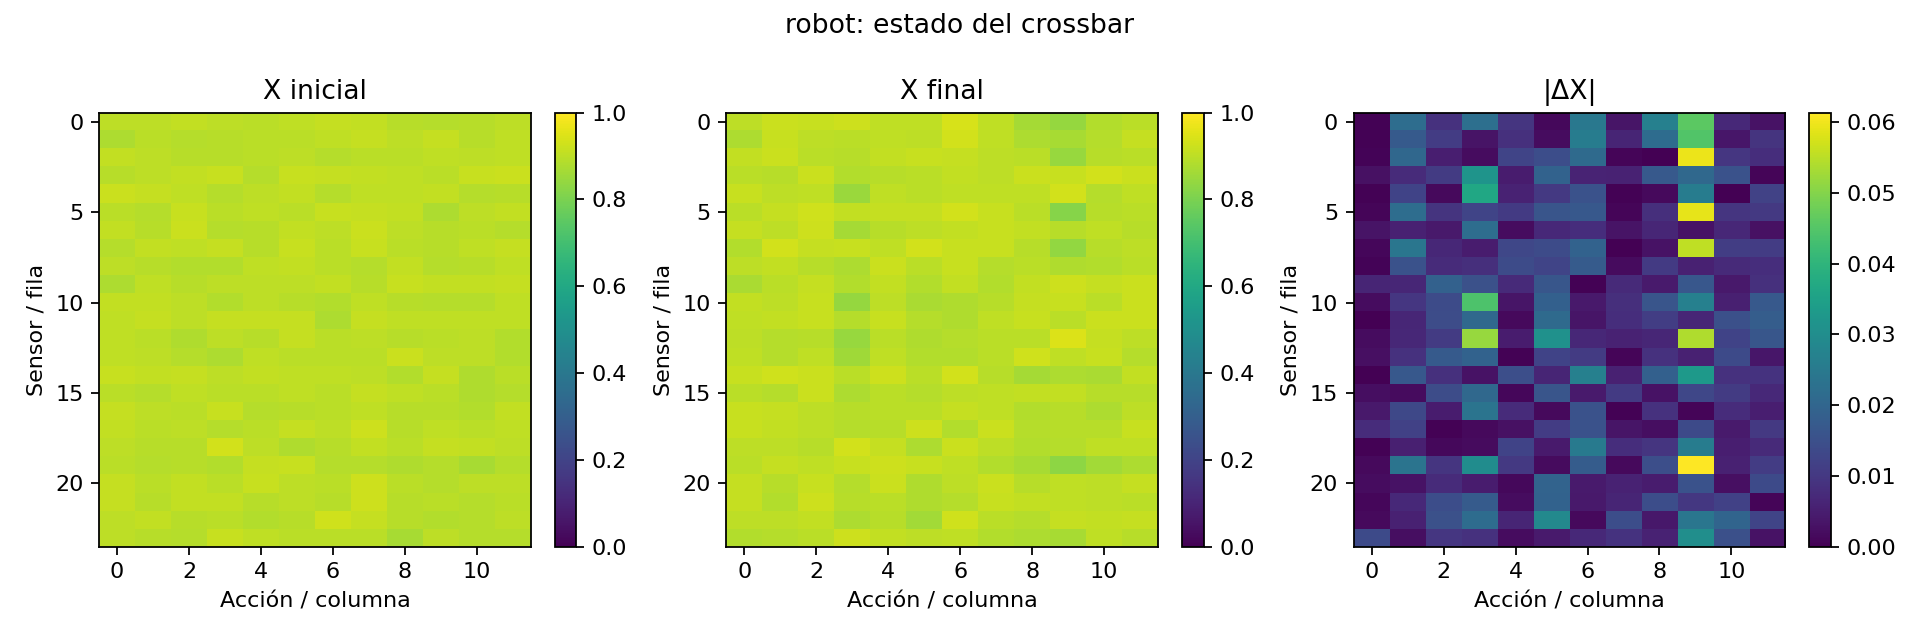
\includegraphics[width=\linewidth,height=0.14\textheight,keepaspectratio]{../../03_EVIDENCIAS/ENTRENAMIENTOS/COMPARATIVA_SEEDS_0_1_X0/runs/robot_rstdp_seed0_X0_0.9/crossbar.png}
\end{minipage}\hfill
\begin{minipage}[t]{0.49\textwidth}
\centering
\textit{Curva de \'exito}\par
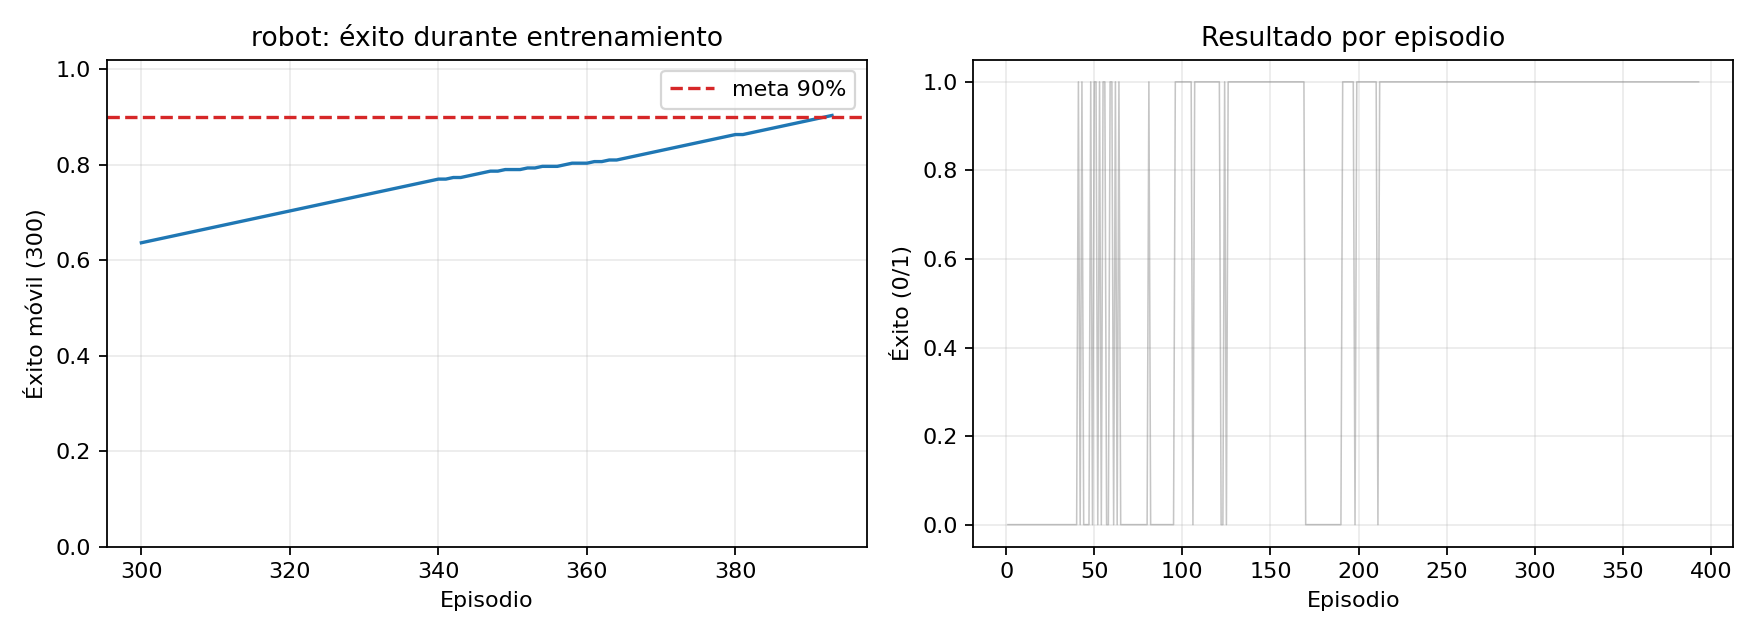
\includegraphics[width=\linewidth,height=0.14\textheight,keepaspectratio]{../../03_EVIDENCIAS/ENTRENAMIENTOS/COMPARATIVA_SEEDS_0_1_X0/runs/robot_rstdp_seed0_X0_0.9/success_curve.png}
\end{minipage}\par\smallskip
\noindent\textbf{CartPole | R-STDP | semilla 1 | $X_0=0.1$}\\
{\scriptsize lote principal; episodios completados: 377; tasa de \'exito en la ventana final: 90.33\%; criterio alcanzado: s\'i.}\par
\noindent\begin{minipage}[t]{0.49\textwidth}
\centering
\textit{Crossbar $X$}\par
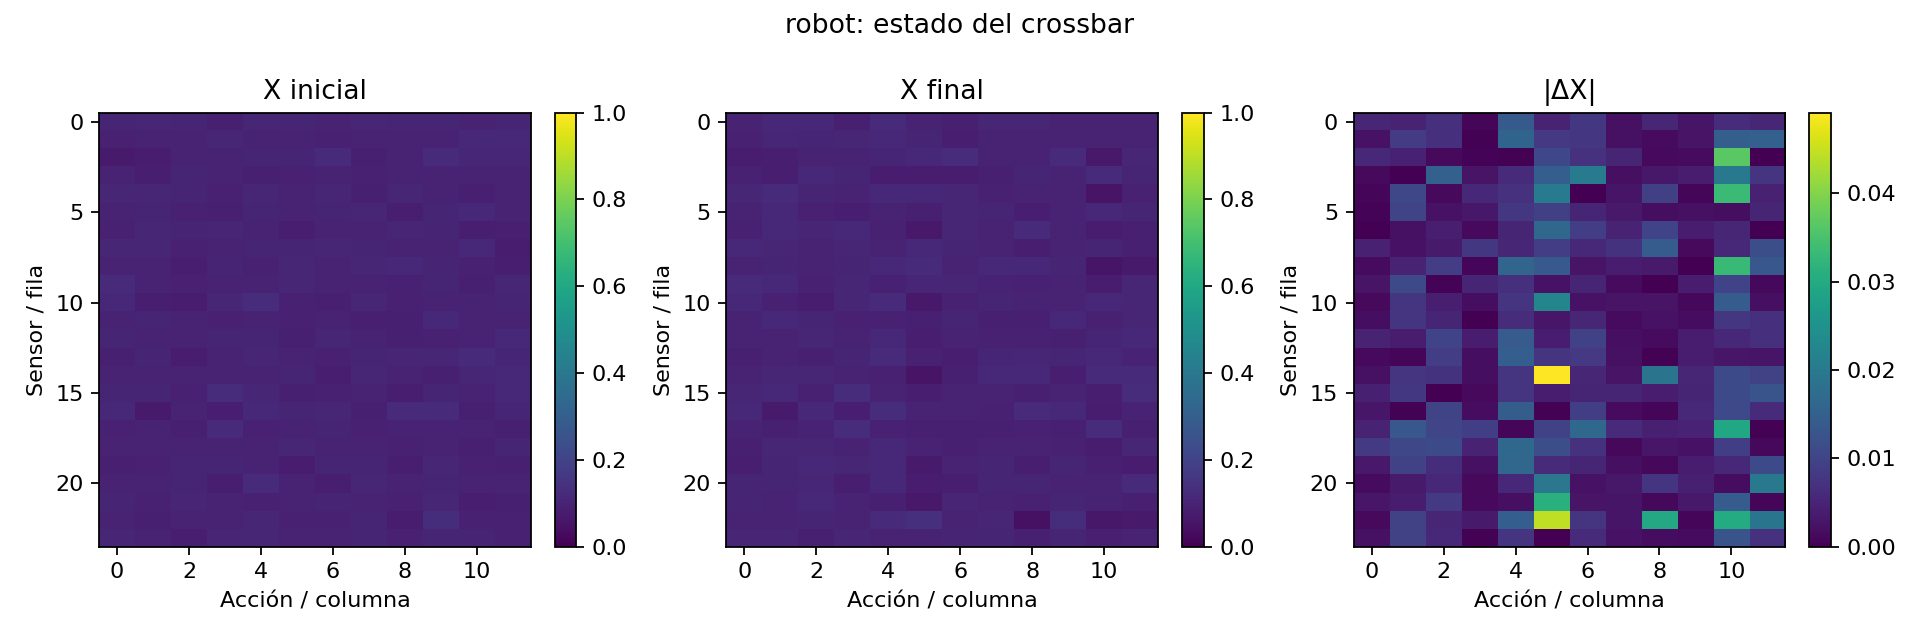
\includegraphics[width=\linewidth,height=0.14\textheight,keepaspectratio]{../../03_EVIDENCIAS/ENTRENAMIENTOS/COMPARATIVA_SEEDS_0_1_X0/runs/robot_rstdp_seed1_X0_0.1/crossbar.png}
\end{minipage}\hfill
\begin{minipage}[t]{0.49\textwidth}
\centering
\textit{Curva de \'exito}\par
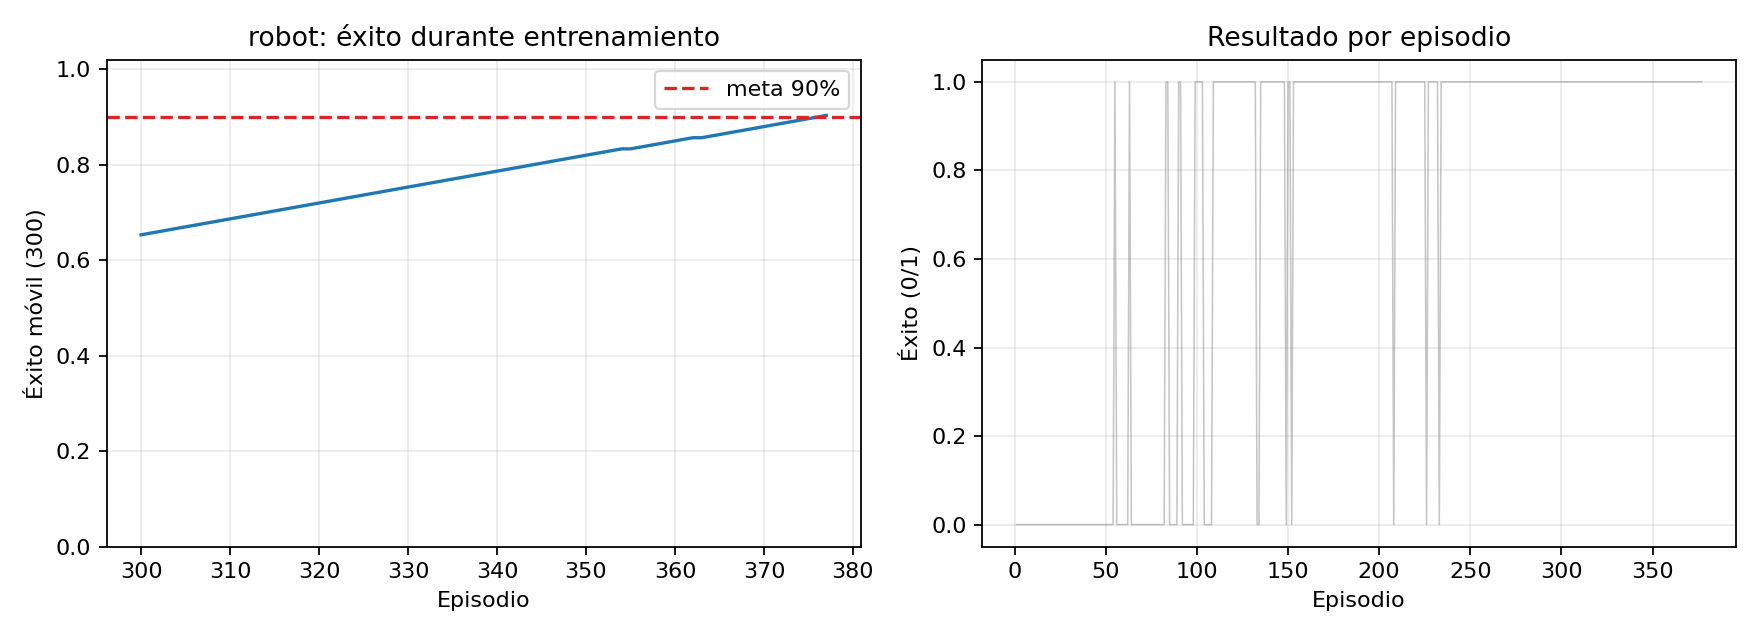
\includegraphics[width=\linewidth,height=0.14\textheight,keepaspectratio]{../../03_EVIDENCIAS/ENTRENAMIENTOS/COMPARATIVA_SEEDS_0_1_X0/runs/robot_rstdp_seed1_X0_0.1/success_curve.png}
\end{minipage}\par\smallskip
\noindent\textbf{CartPole | R-STDP | semilla 1 | $X_0=0.9$}\\
{\scriptsize lote principal; episodios completados: 1199; tasa de \'exito en la ventana final: 90.33\%; criterio alcanzado: s\'i.}\par
\noindent\begin{minipage}[t]{0.49\textwidth}
\centering
\textit{Crossbar $X$}\par
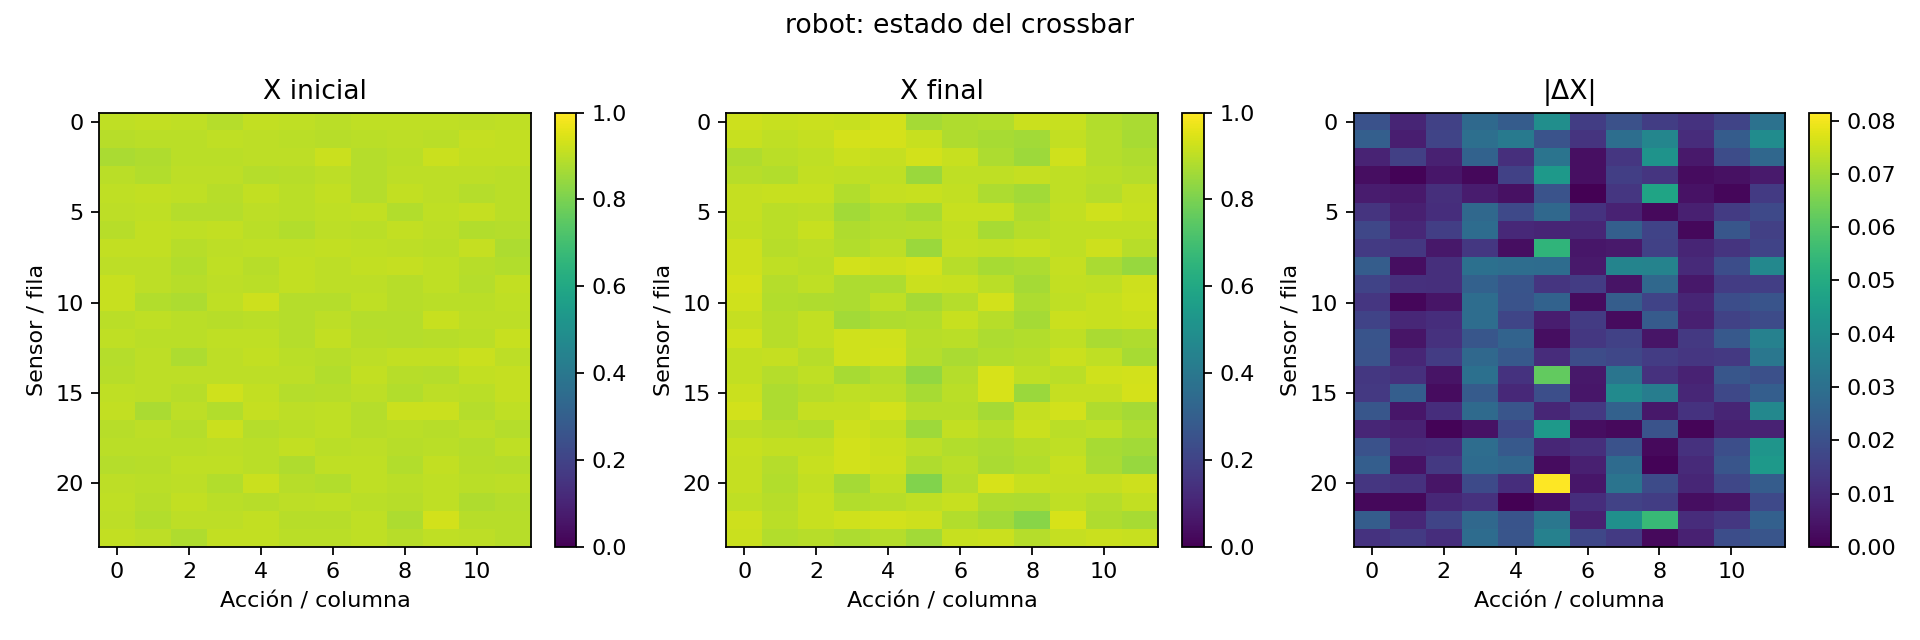
\includegraphics[width=\linewidth,height=0.14\textheight,keepaspectratio]{../../03_EVIDENCIAS/ENTRENAMIENTOS/COMPARATIVA_SEEDS_0_1_X0/runs/robot_rstdp_seed1_X0_0.9/crossbar.png}
\end{minipage}\hfill
\begin{minipage}[t]{0.49\textwidth}
\centering
\textit{Curva de \'exito}\par
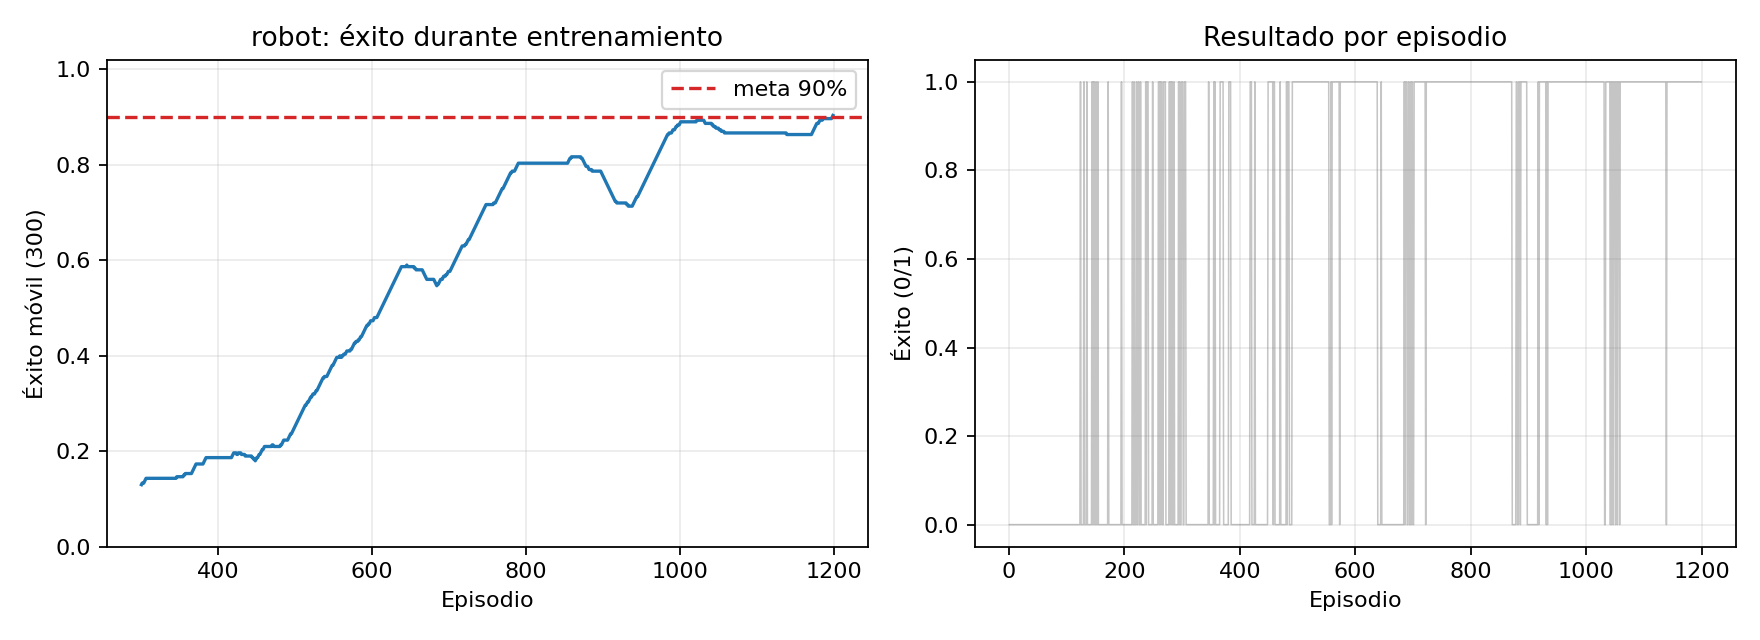
\includegraphics[width=\linewidth,height=0.14\textheight,keepaspectratio]{../../03_EVIDENCIAS/ENTRENAMIENTOS/COMPARATIVA_SEEDS_0_1_X0/runs/robot_rstdp_seed1_X0_0.9/success_curve.png}
\end{minipage}\par\smallskip
\clearpage
\noindent\textbf{Visi\'on | REINFORCE | semilla 0 | $X_0=0.1$}\\
{\scriptsize lote principal; episodios completados: 586; tasa de \'exito en la ventana final: 90.33\%; criterio alcanzado: s\'i.}\par
\noindent\begin{minipage}[t]{0.49\textwidth}
\centering
\textit{Crossbar $X$}\par
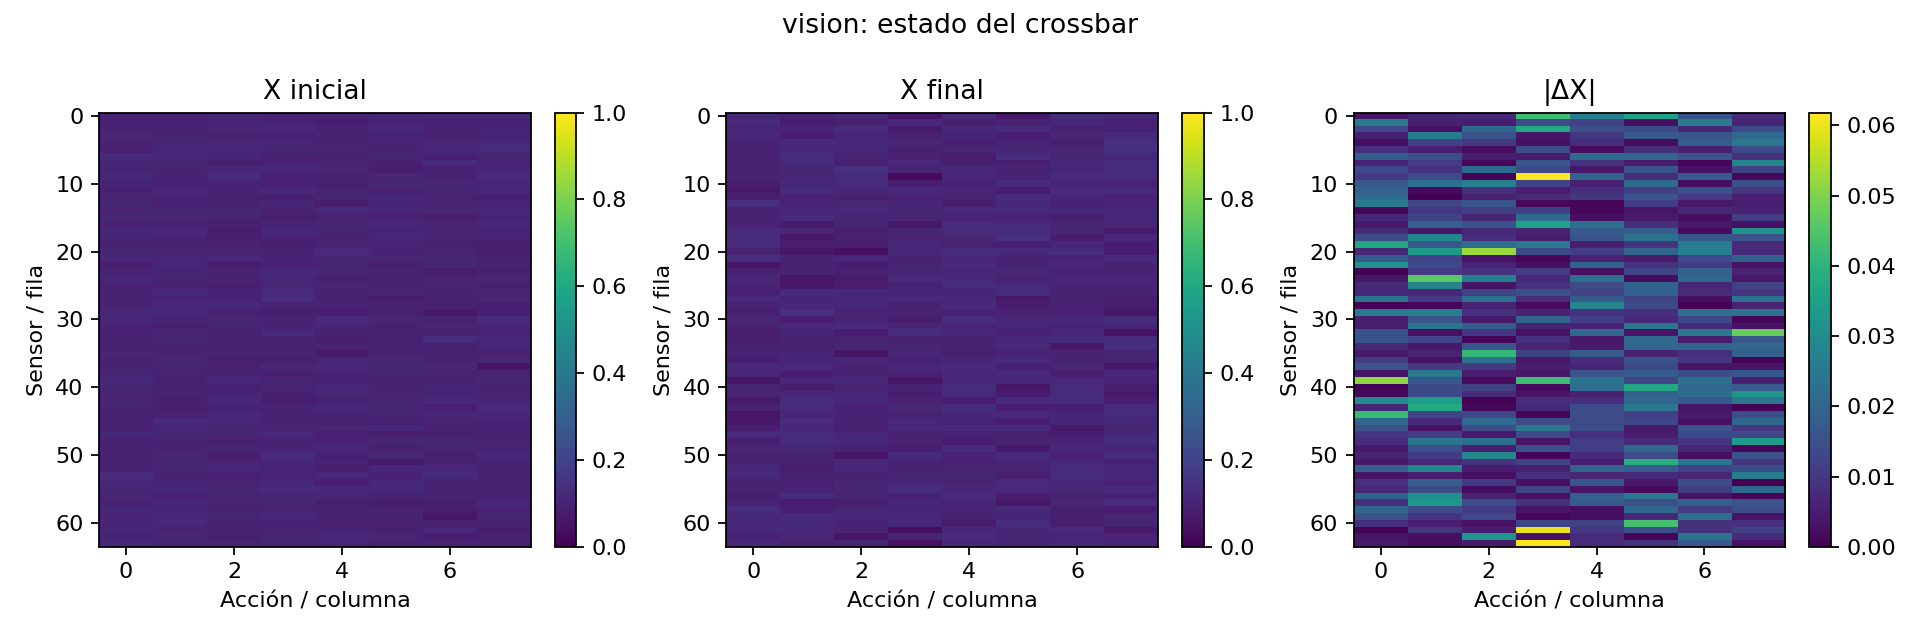
\includegraphics[width=\linewidth,height=0.14\textheight,keepaspectratio]{../../03_EVIDENCIAS/ENTRENAMIENTOS/COMPARATIVA_SEEDS_0_1_X0/runs/vision_reinforce_seed0_X0_0.1/crossbar.png}
\end{minipage}\hfill
\begin{minipage}[t]{0.49\textwidth}
\centering
\textit{Curva de \'exito}\par
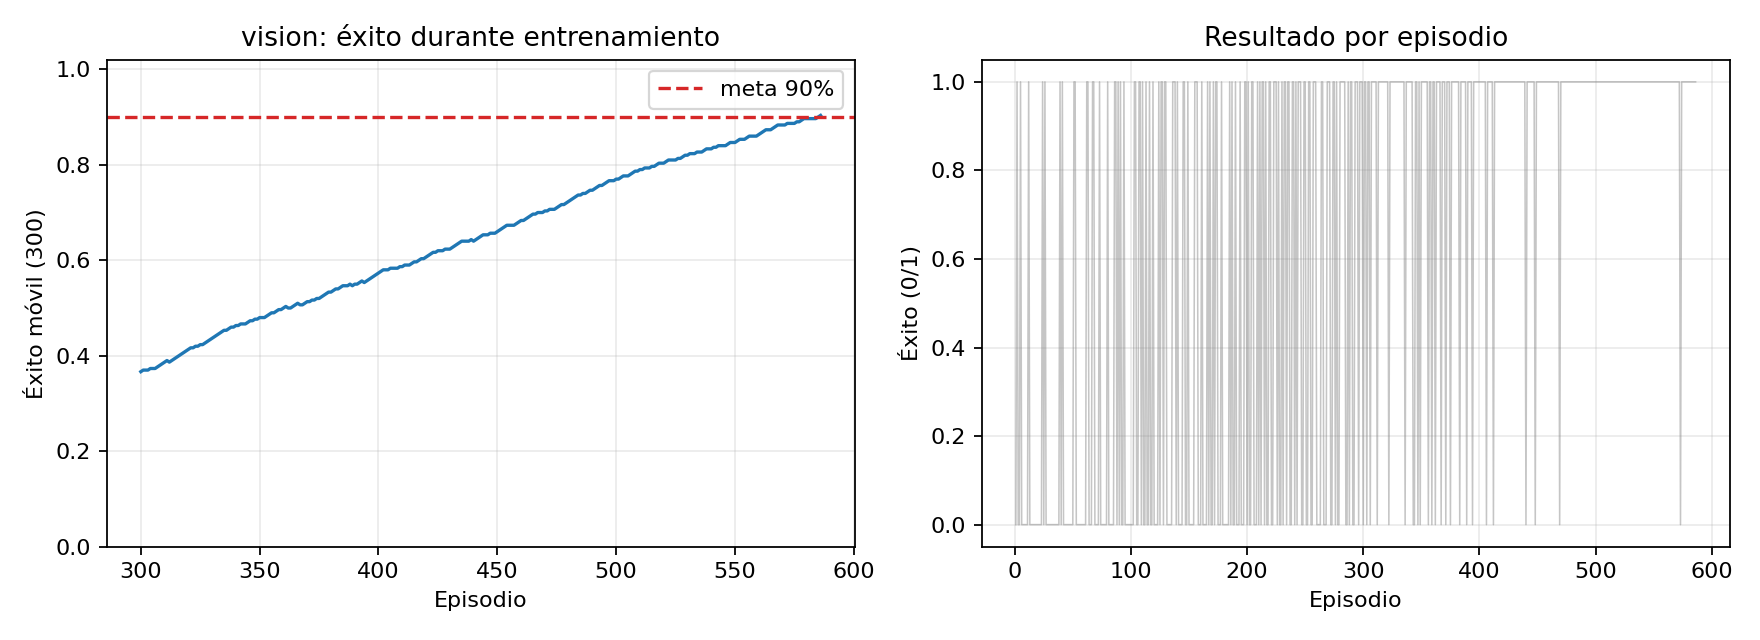
\includegraphics[width=\linewidth,height=0.14\textheight,keepaspectratio]{../../03_EVIDENCIAS/ENTRENAMIENTOS/COMPARATIVA_SEEDS_0_1_X0/runs/vision_reinforce_seed0_X0_0.1/success_curve.png}
\end{minipage}\par\smallskip
\noindent\textbf{Visi\'on | REINFORCE | semilla 0 | $X_0=0.9$}\\
{\scriptsize lote principal; episodios completados: 1357; tasa de \'exito en la ventana final: 90.33\%; criterio alcanzado: s\'i.}\par
\noindent\begin{minipage}[t]{0.49\textwidth}
\centering
\textit{Crossbar $X$}\par
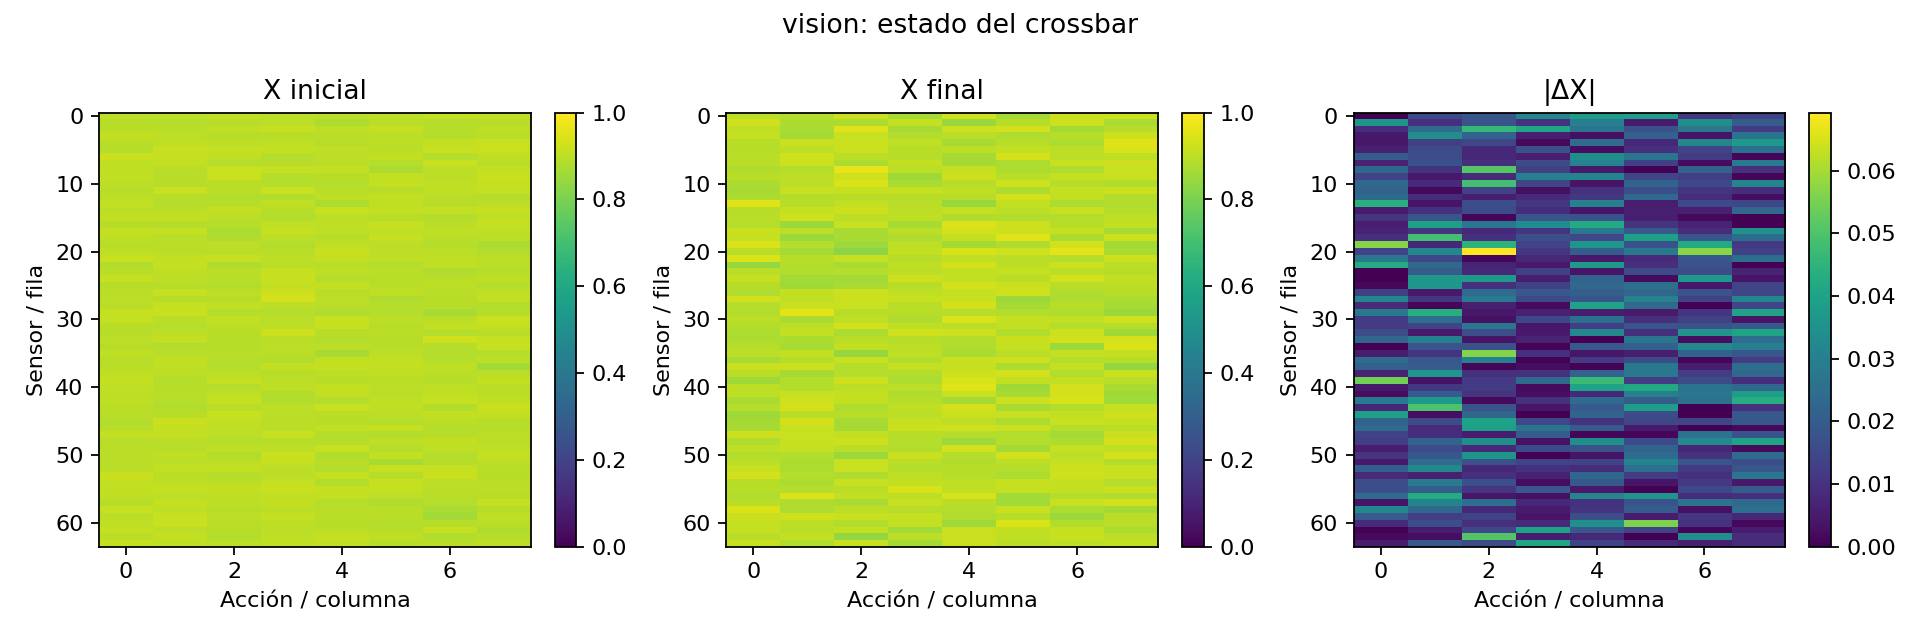
\includegraphics[width=\linewidth,height=0.14\textheight,keepaspectratio]{../../03_EVIDENCIAS/ENTRENAMIENTOS/COMPARATIVA_SEEDS_0_1_X0/runs/vision_reinforce_seed0_X0_0.9/crossbar.png}
\end{minipage}\hfill
\begin{minipage}[t]{0.49\textwidth}
\centering
\textit{Curva de \'exito}\par
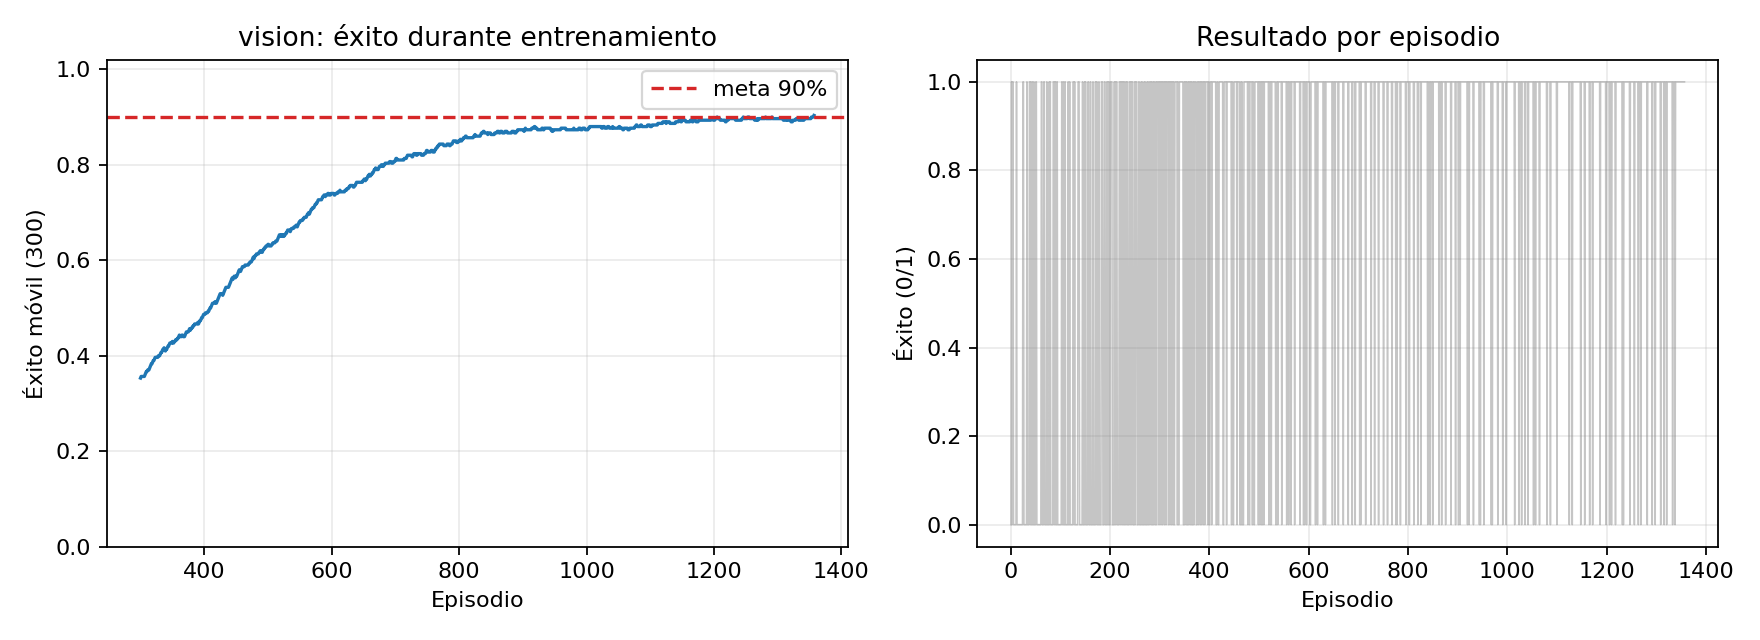
\includegraphics[width=\linewidth,height=0.14\textheight,keepaspectratio]{../../03_EVIDENCIAS/ENTRENAMIENTOS/COMPARATIVA_SEEDS_0_1_X0/runs/vision_reinforce_seed0_X0_0.9/success_curve.png}
\end{minipage}\par\smallskip
\noindent\textbf{Visi\'on | REINFORCE | semilla 1 | $X_0=0.1$}\\
{\scriptsize lote principal; episodios completados: 976; tasa de \'exito en la ventana final: 90.33\%; criterio alcanzado: s\'i.}\par
\noindent\begin{minipage}[t]{0.49\textwidth}
\centering
\textit{Crossbar $X$}\par
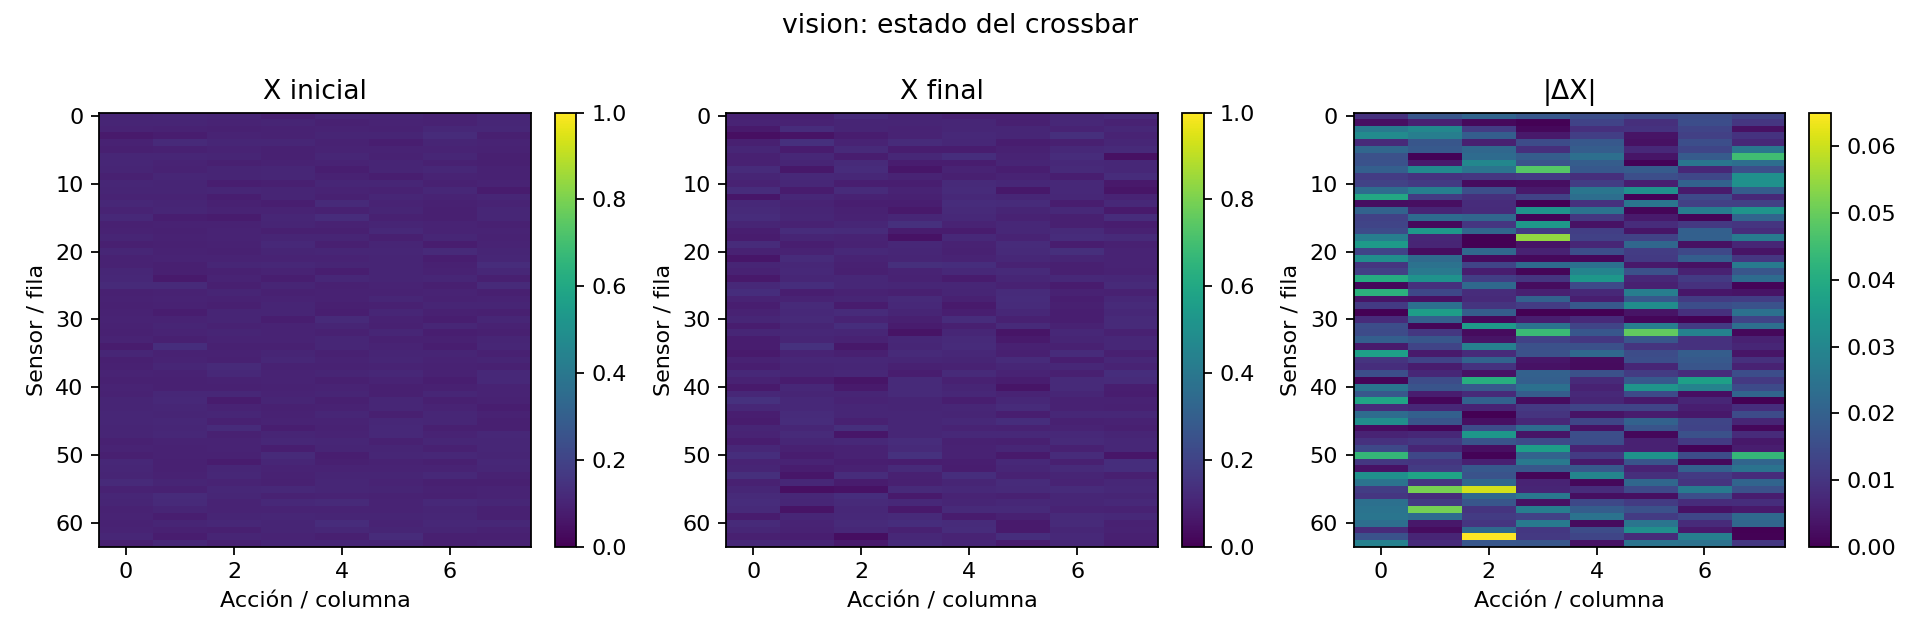
\includegraphics[width=\linewidth,height=0.14\textheight,keepaspectratio]{../../03_EVIDENCIAS/ENTRENAMIENTOS/COMPARATIVA_SEEDS_0_1_X0/runs/vision_reinforce_seed1_X0_0.1/crossbar.png}
\end{minipage}\hfill
\begin{minipage}[t]{0.49\textwidth}
\centering
\textit{Curva de \'exito}\par
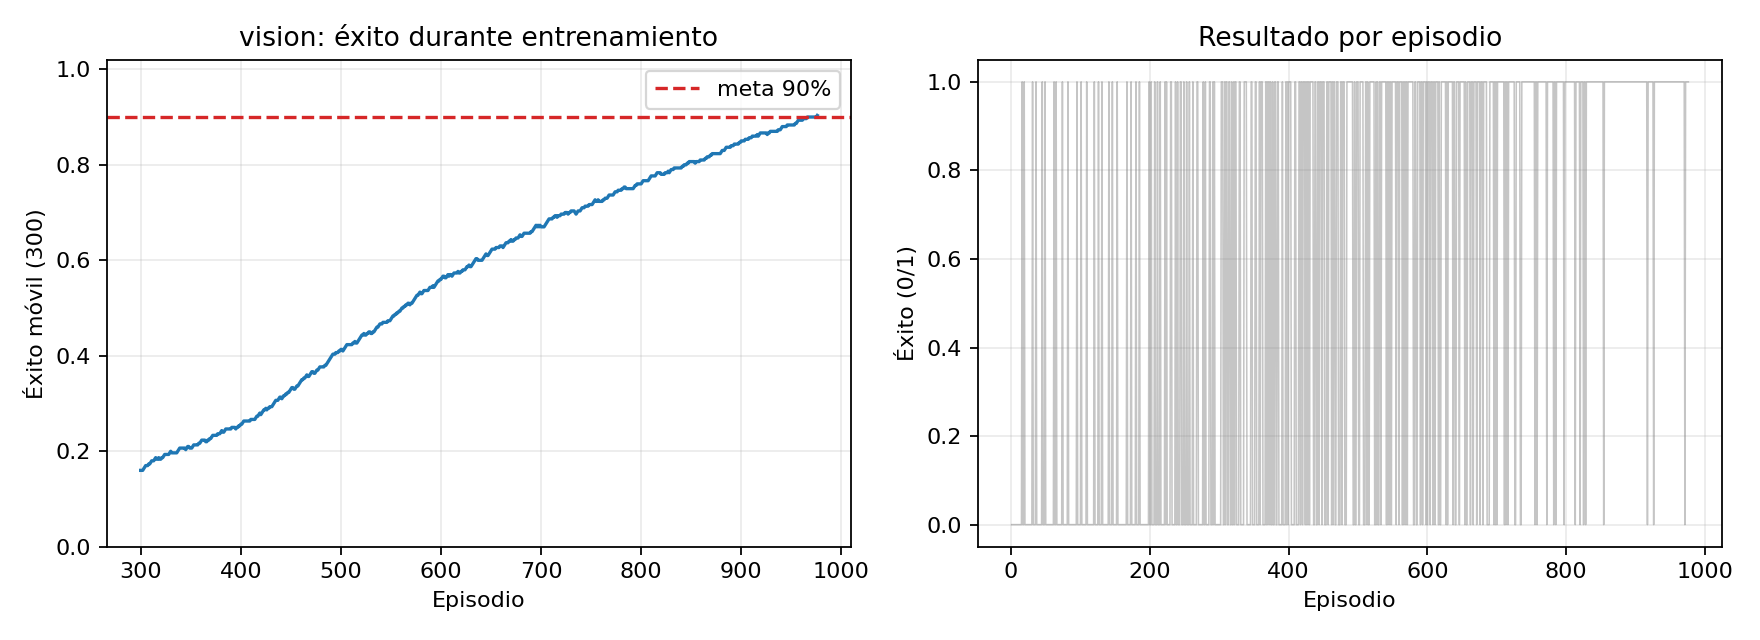
\includegraphics[width=\linewidth,height=0.14\textheight,keepaspectratio]{../../03_EVIDENCIAS/ENTRENAMIENTOS/COMPARATIVA_SEEDS_0_1_X0/runs/vision_reinforce_seed1_X0_0.1/success_curve.png}
\end{minipage}\par\smallskip
\noindent\textbf{Visi\'on | REINFORCE | semilla 1 | $X_0=0.9$}\\
{\scriptsize lote principal; episodios completados: 1008; tasa de \'exito en la ventana final: 90.33\%; criterio alcanzado: s\'i.}\par
\noindent\begin{minipage}[t]{0.49\textwidth}
\centering
\textit{Crossbar $X$}\par
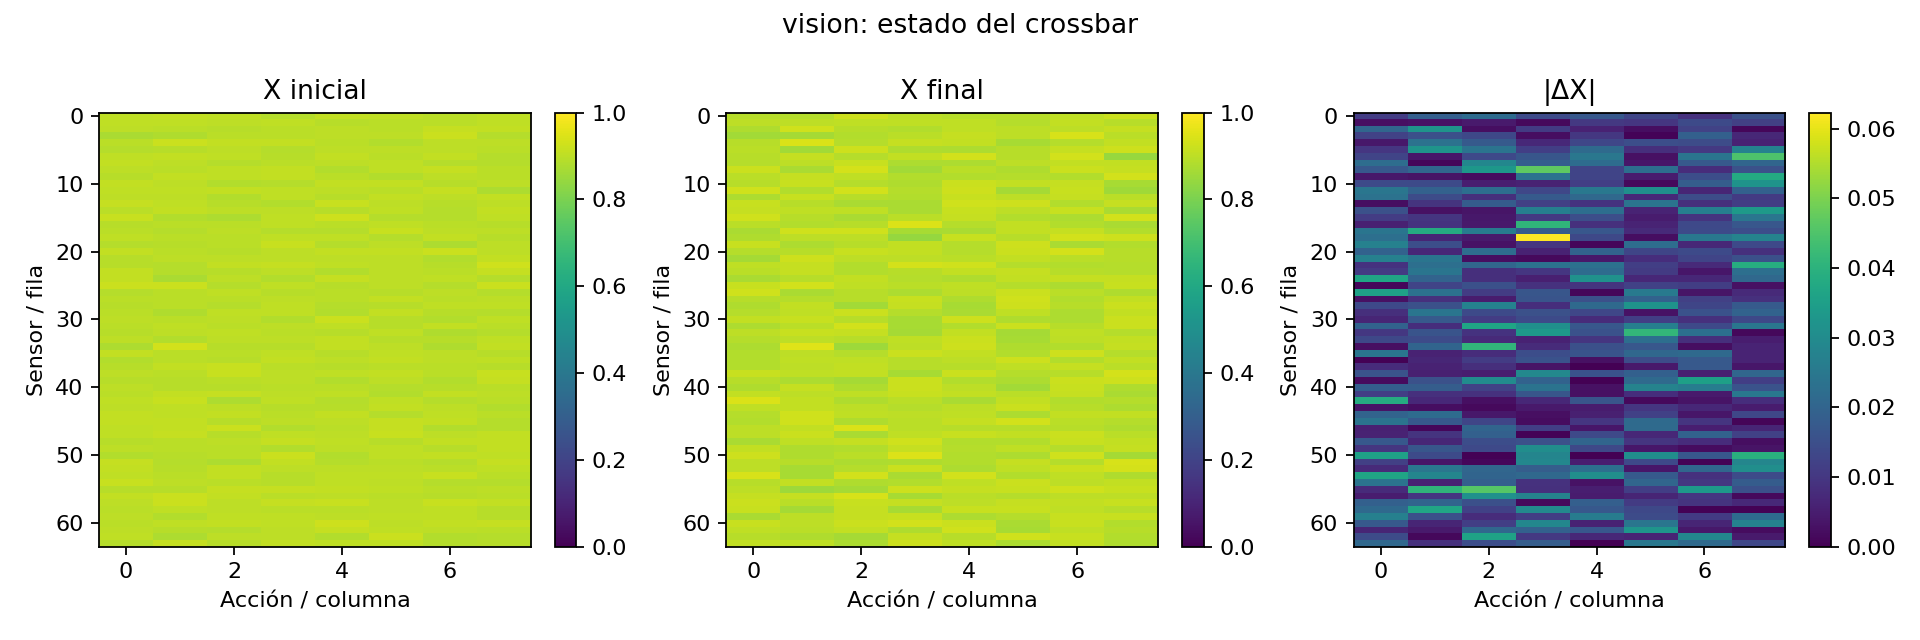
\includegraphics[width=\linewidth,height=0.14\textheight,keepaspectratio]{../../03_EVIDENCIAS/ENTRENAMIENTOS/COMPARATIVA_SEEDS_0_1_X0/runs/vision_reinforce_seed1_X0_0.9/crossbar.png}
\end{minipage}\hfill
\begin{minipage}[t]{0.49\textwidth}
\centering
\textit{Curva de \'exito}\par
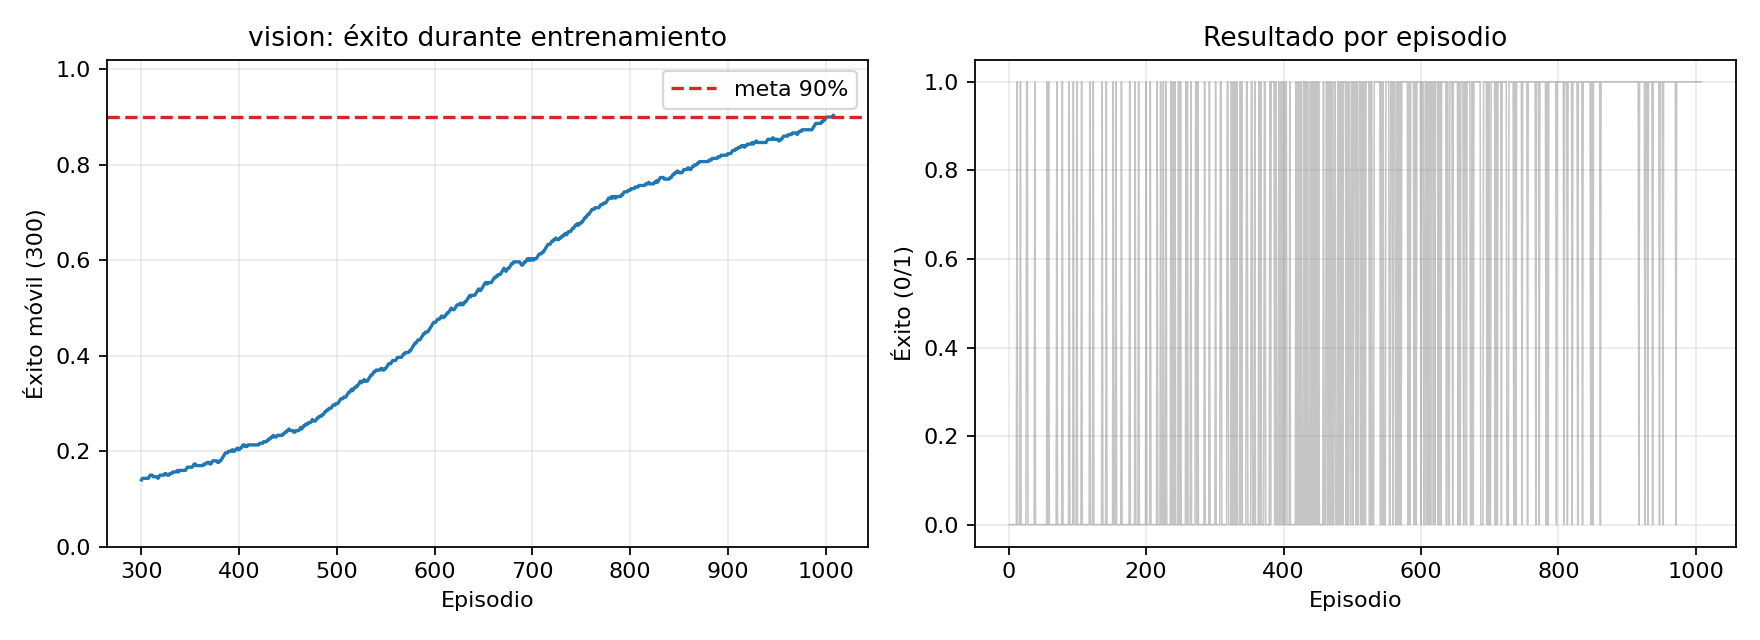
\includegraphics[width=\linewidth,height=0.14\textheight,keepaspectratio]{../../03_EVIDENCIAS/ENTRENAMIENTOS/COMPARATIVA_SEEDS_0_1_X0/runs/vision_reinforce_seed1_X0_0.9/success_curve.png}
\end{minipage}\par\smallskip
\clearpage
\noindent\textbf{Visi\'on | R-STDP | semilla 0 | $X_0=0.1$}\\
{\scriptsize lote principal; episodios completados: 2566; tasa de \'exito en la ventana final: 90.33\%; criterio alcanzado: s\'i.}\par
\noindent\begin{minipage}[t]{0.49\textwidth}
\centering
\textit{Crossbar $X$}\par
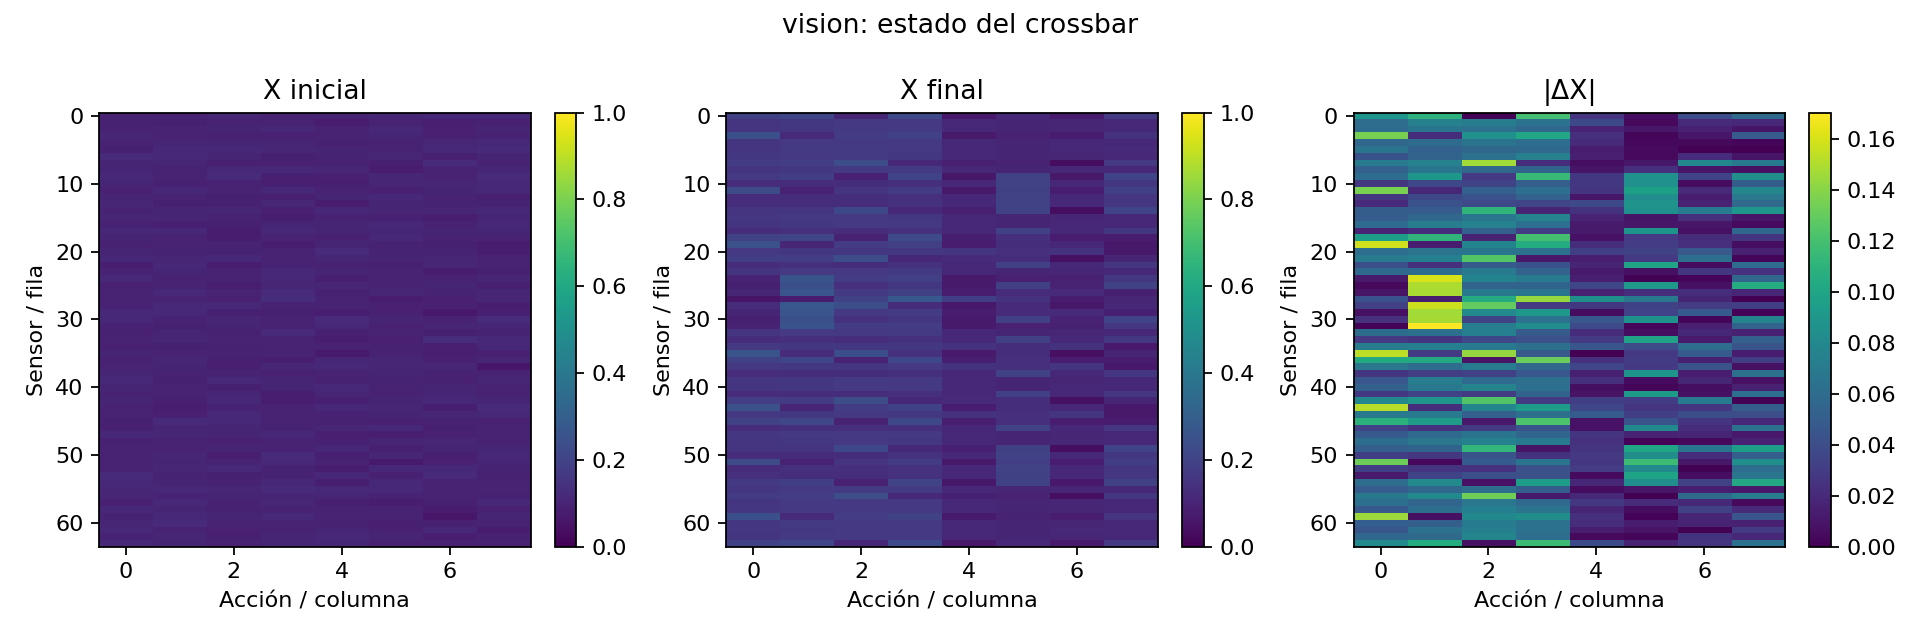
\includegraphics[width=\linewidth,height=0.14\textheight,keepaspectratio]{../../03_EVIDENCIAS/ENTRENAMIENTOS/COMPARATIVA_SEEDS_0_1_X0/runs/vision_rstdp_seed0_X0_0.1/crossbar.png}
\end{minipage}\hfill
\begin{minipage}[t]{0.49\textwidth}
\centering
\textit{Curva de \'exito}\par
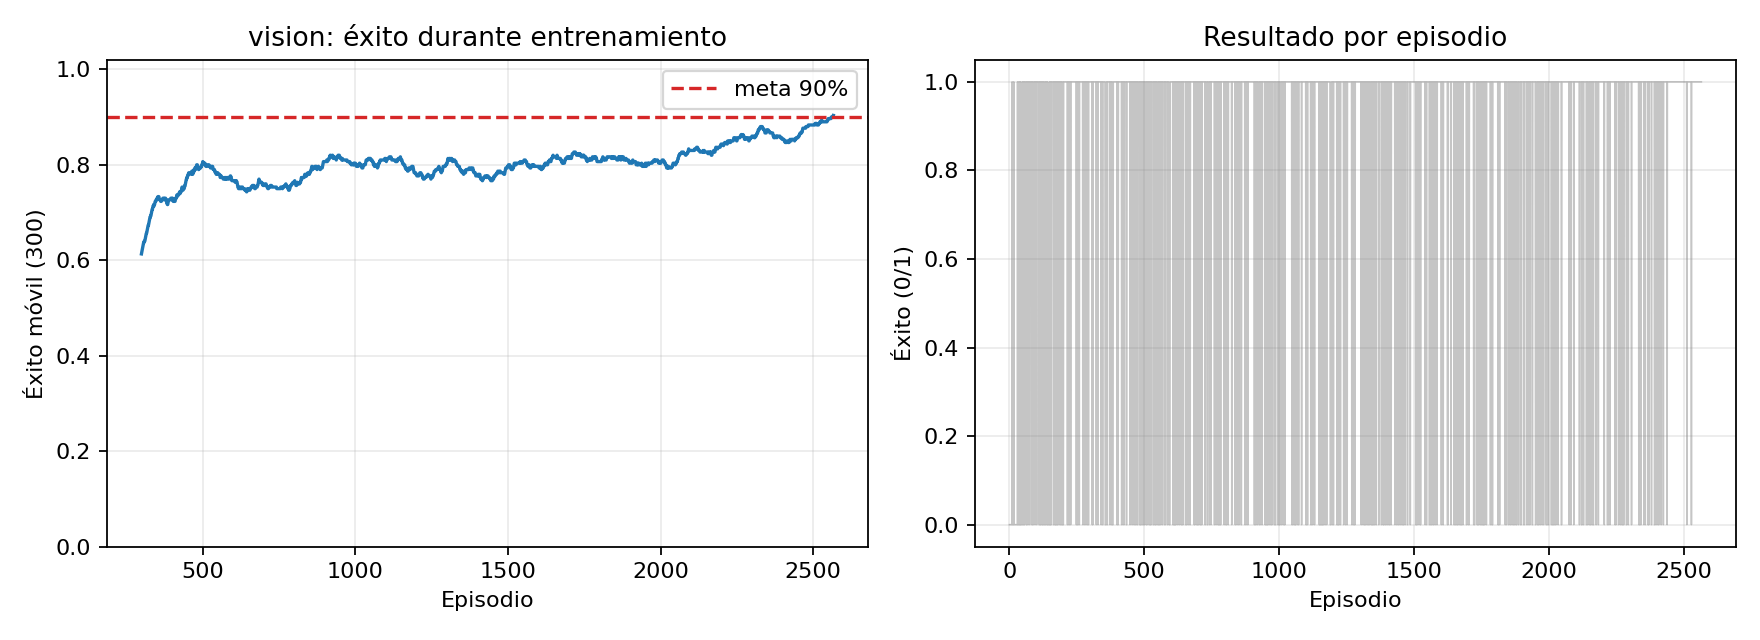
\includegraphics[width=\linewidth,height=0.14\textheight,keepaspectratio]{../../03_EVIDENCIAS/ENTRENAMIENTOS/COMPARATIVA_SEEDS_0_1_X0/runs/vision_rstdp_seed0_X0_0.1/success_curve.png}
\end{minipage}\par\smallskip
\noindent\textbf{Visi\'on | R-STDP | semilla 0 | $X_0=0.9$}\\
{\scriptsize lote principal; episodios completados: 773; tasa de \'exito en la ventana final: 90.33\%; criterio alcanzado: s\'i.}\par
\noindent\begin{minipage}[t]{0.49\textwidth}
\centering
\textit{Crossbar $X$}\par
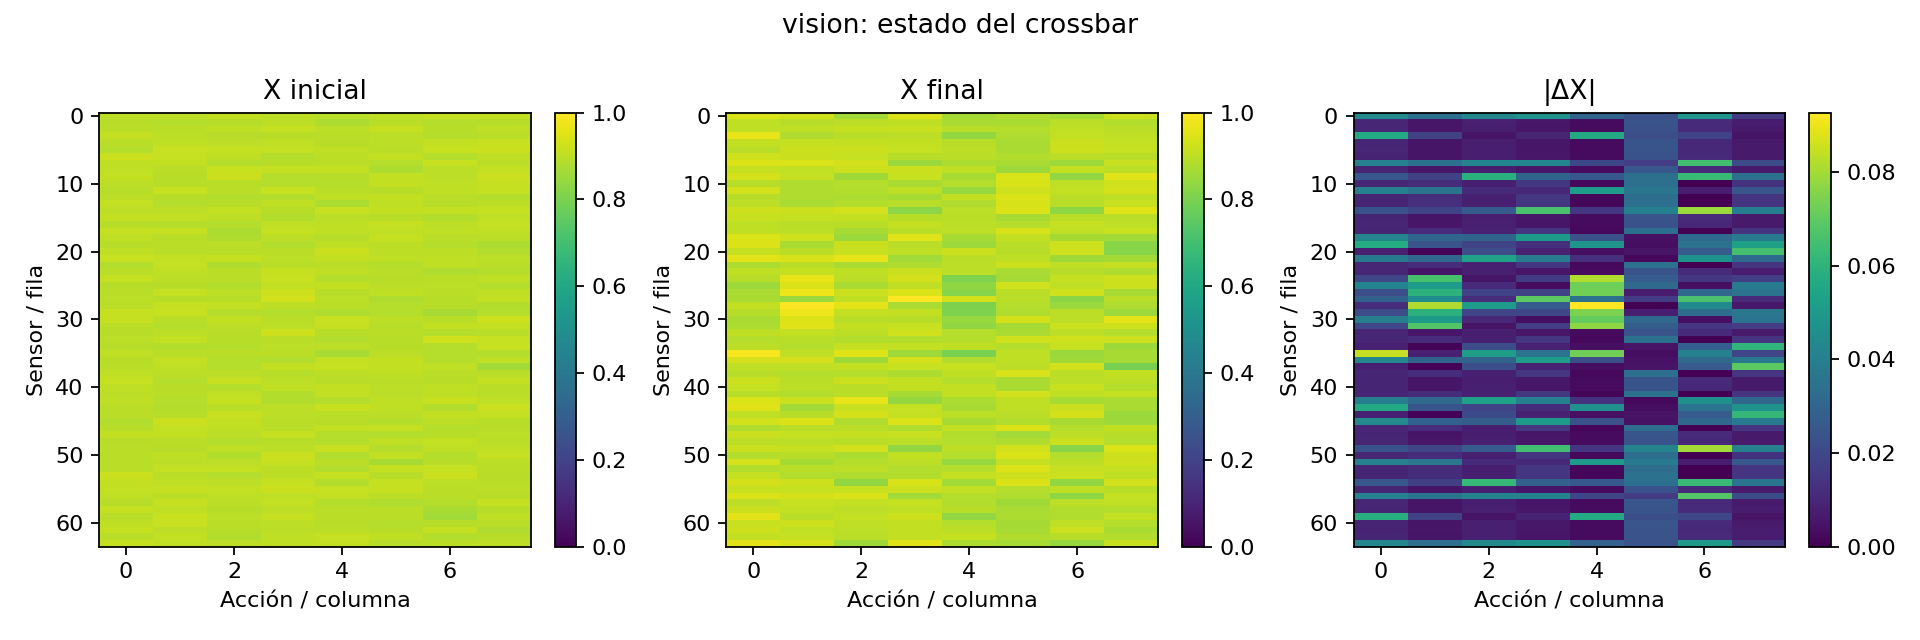
\includegraphics[width=\linewidth,height=0.14\textheight,keepaspectratio]{../../03_EVIDENCIAS/ENTRENAMIENTOS/COMPARATIVA_SEEDS_0_1_X0/runs/vision_rstdp_seed0_X0_0.9/crossbar.png}
\end{minipage}\hfill
\begin{minipage}[t]{0.49\textwidth}
\centering
\textit{Curva de \'exito}\par
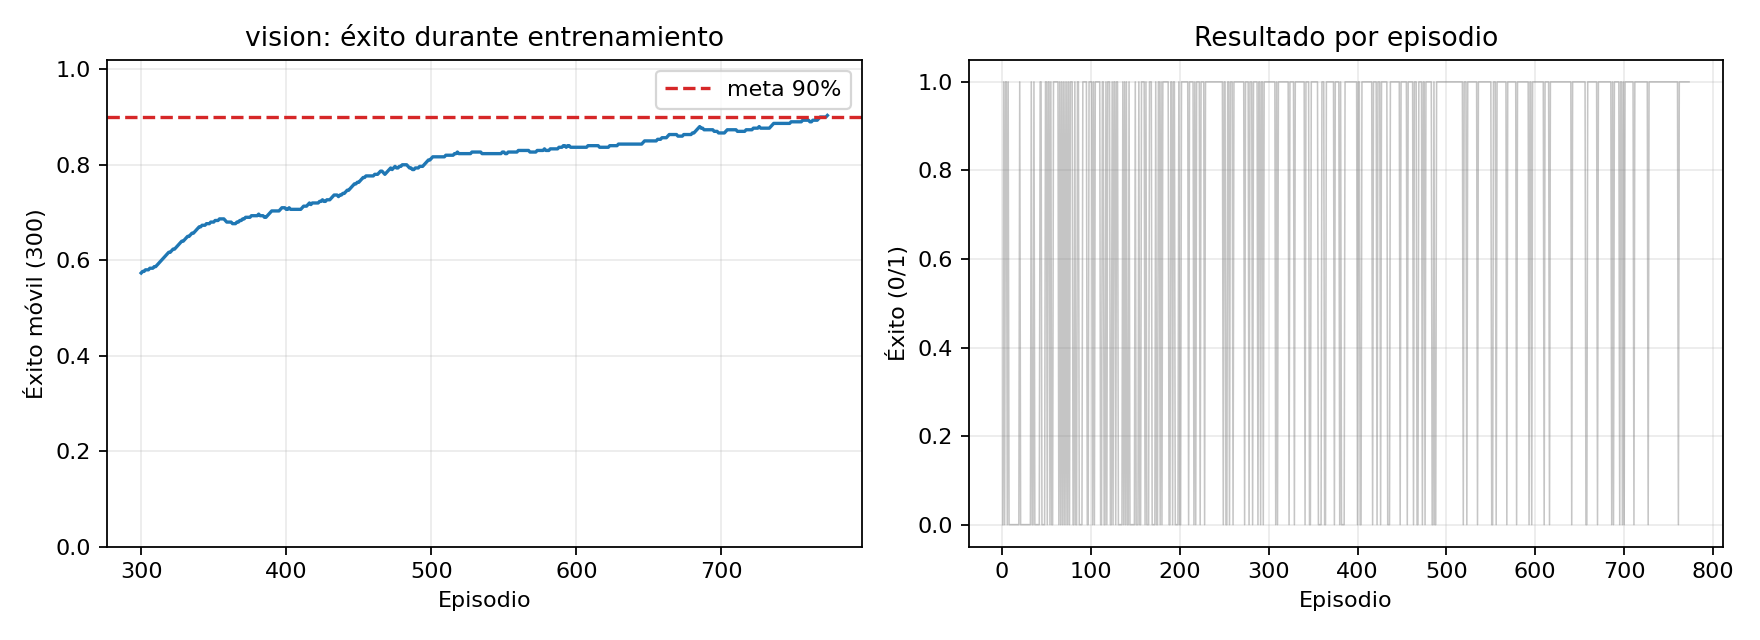
\includegraphics[width=\linewidth,height=0.14\textheight,keepaspectratio]{../../03_EVIDENCIAS/ENTRENAMIENTOS/COMPARATIVA_SEEDS_0_1_X0/runs/vision_rstdp_seed0_X0_0.9/success_curve.png}
\end{minipage}\par\smallskip
\noindent\textbf{Visi\'on | R-STDP | semilla 1 | $X_0=0.1$}\\
{\scriptsize lote principal; episodios completados: 2951; tasa de \'exito en la ventana final: 90.33\%; criterio alcanzado: s\'i.}\par
\noindent\begin{minipage}[t]{0.49\textwidth}
\centering
\textit{Crossbar $X$}\par
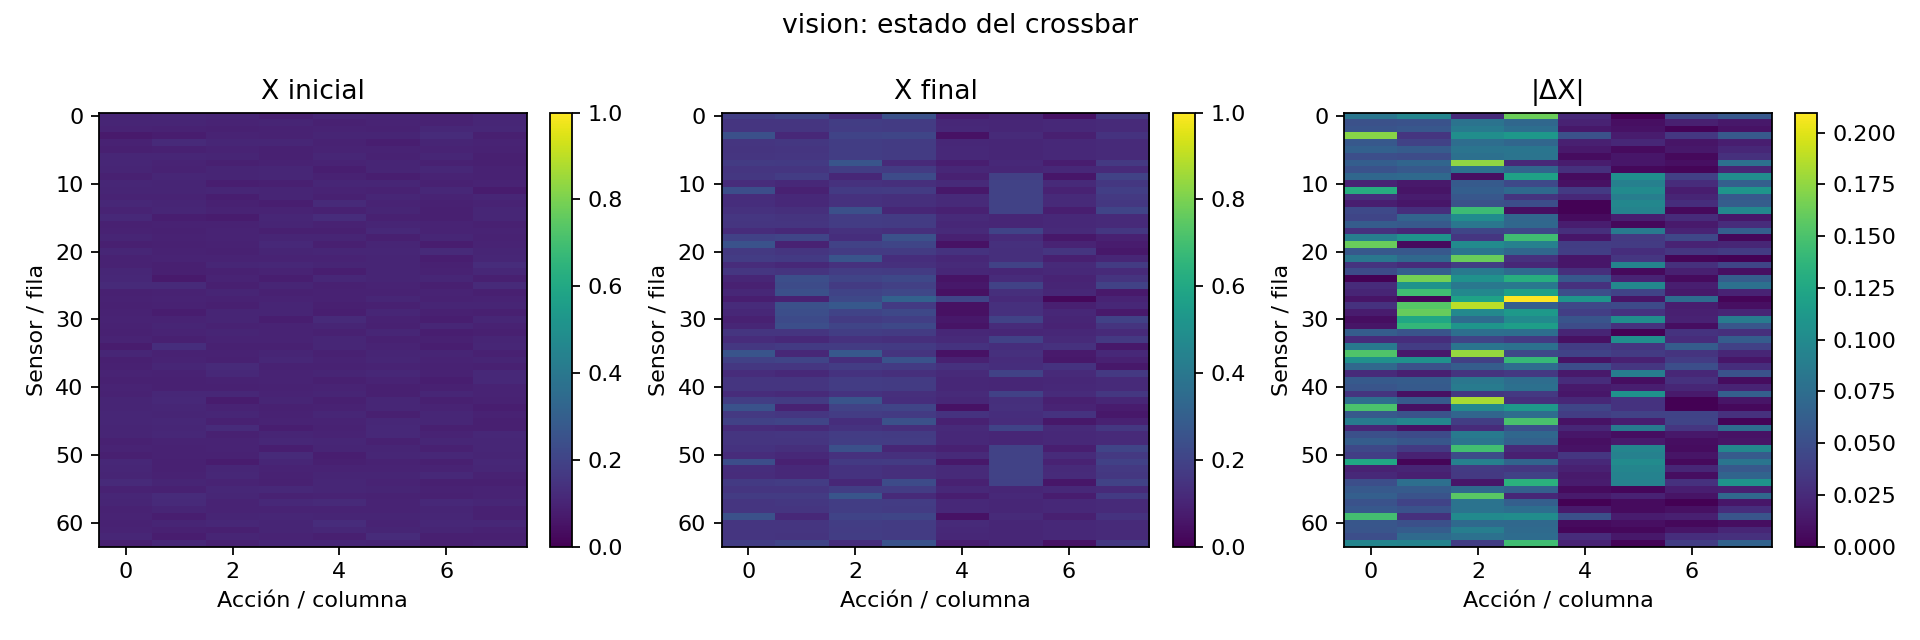
\includegraphics[width=\linewidth,height=0.14\textheight,keepaspectratio]{../../03_EVIDENCIAS/ENTRENAMIENTOS/COMPARATIVA_SEEDS_0_1_X0/runs/vision_rstdp_seed1_X0_0.1/crossbar.png}
\end{minipage}\hfill
\begin{minipage}[t]{0.49\textwidth}
\centering
\textit{Curva de \'exito}\par
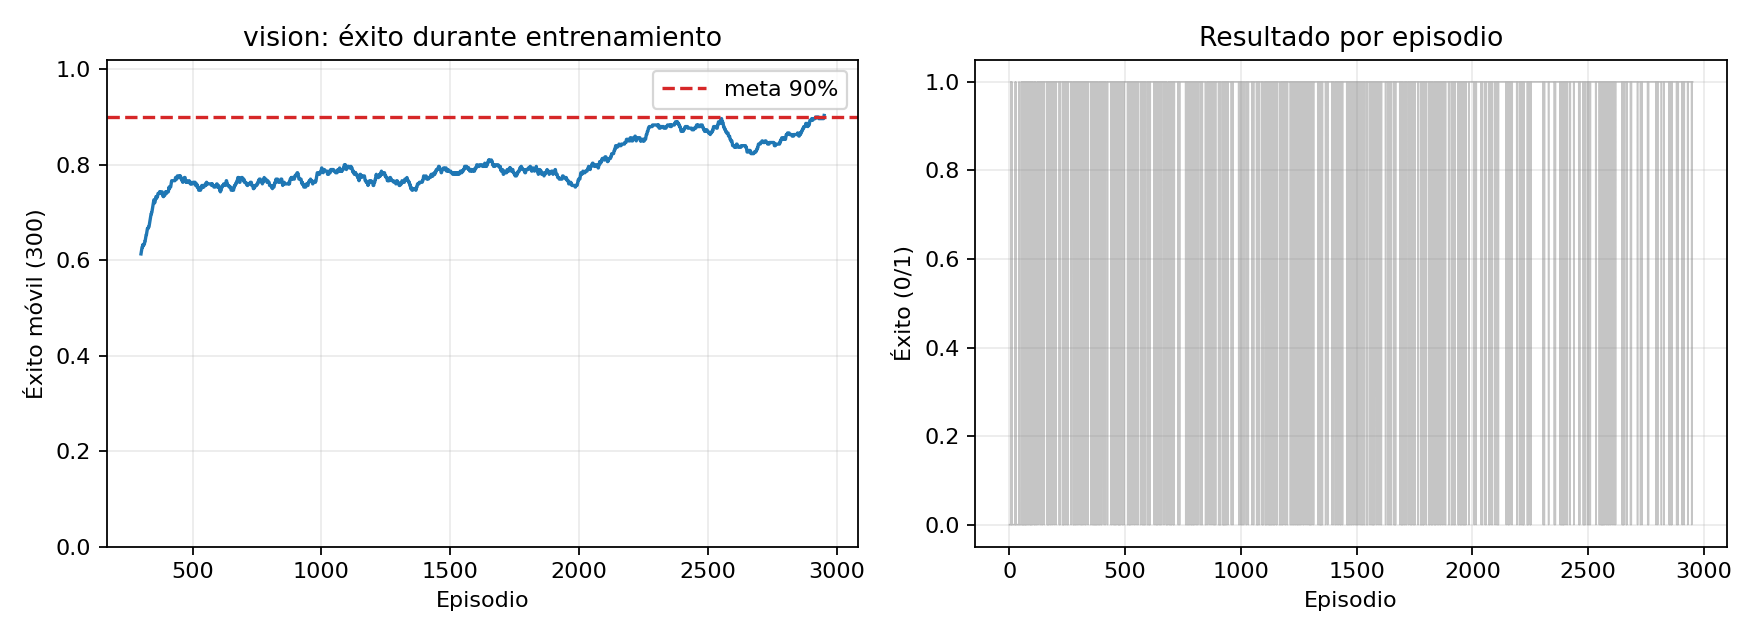
\includegraphics[width=\linewidth,height=0.14\textheight,keepaspectratio]{../../03_EVIDENCIAS/ENTRENAMIENTOS/COMPARATIVA_SEEDS_0_1_X0/runs/vision_rstdp_seed1_X0_0.1/success_curve.png}
\end{minipage}\par\smallskip
\noindent\textbf{Visi\'on | R-STDP | semilla 1 | $X_0=0.9$}\\
{\scriptsize lote principal; episodios completados: 470; tasa de \'exito en la ventana final: 90.33\%; criterio alcanzado: s\'i.}\par
\noindent\begin{minipage}[t]{0.49\textwidth}
\centering
\textit{Crossbar $X$}\par
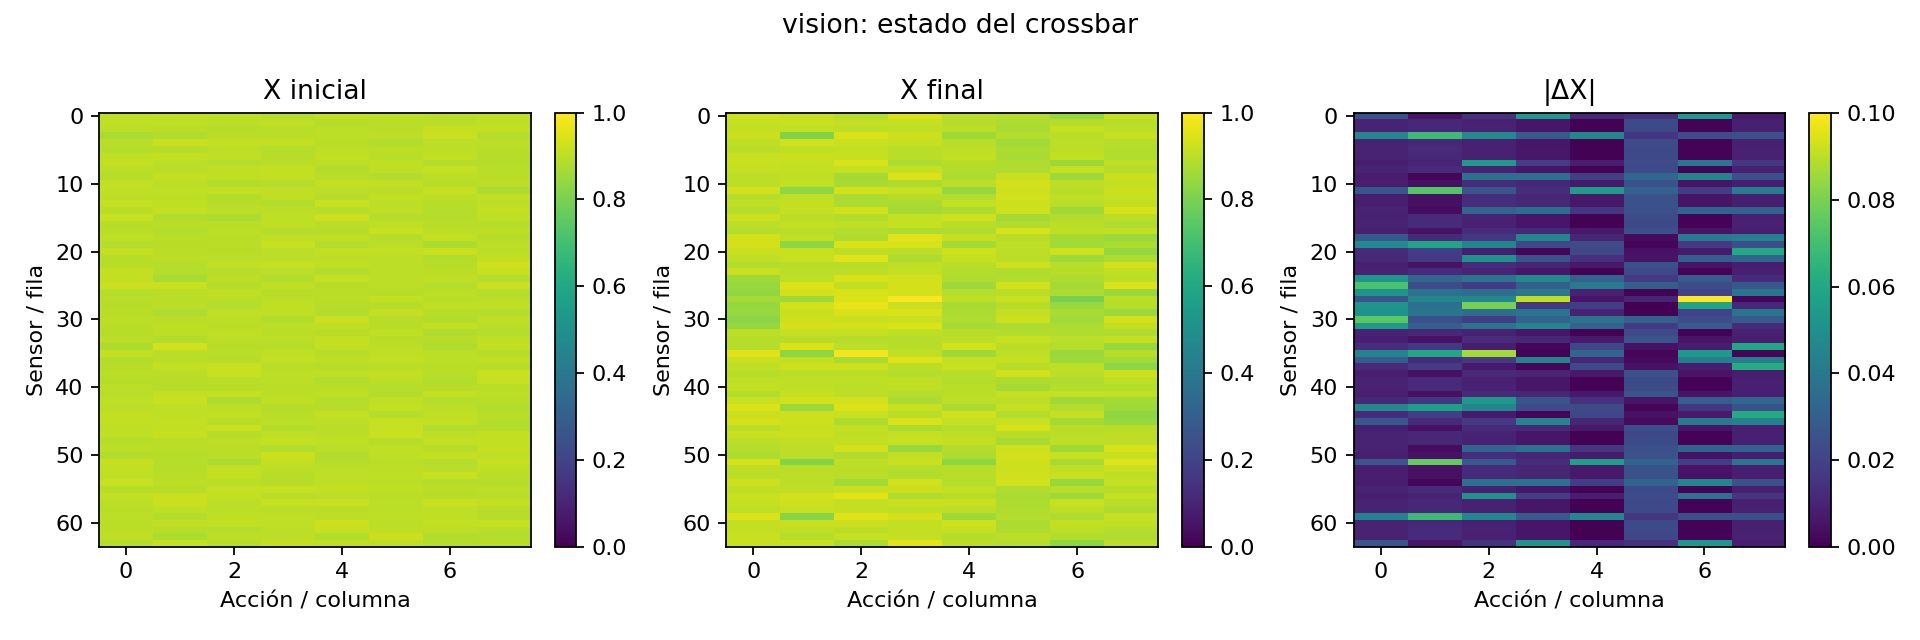
\includegraphics[width=\linewidth,height=0.14\textheight,keepaspectratio]{../../03_EVIDENCIAS/ENTRENAMIENTOS/COMPARATIVA_SEEDS_0_1_X0/runs/vision_rstdp_seed1_X0_0.9/crossbar.png}
\end{minipage}\hfill
\begin{minipage}[t]{0.49\textwidth}
\centering
\textit{Curva de \'exito}\par
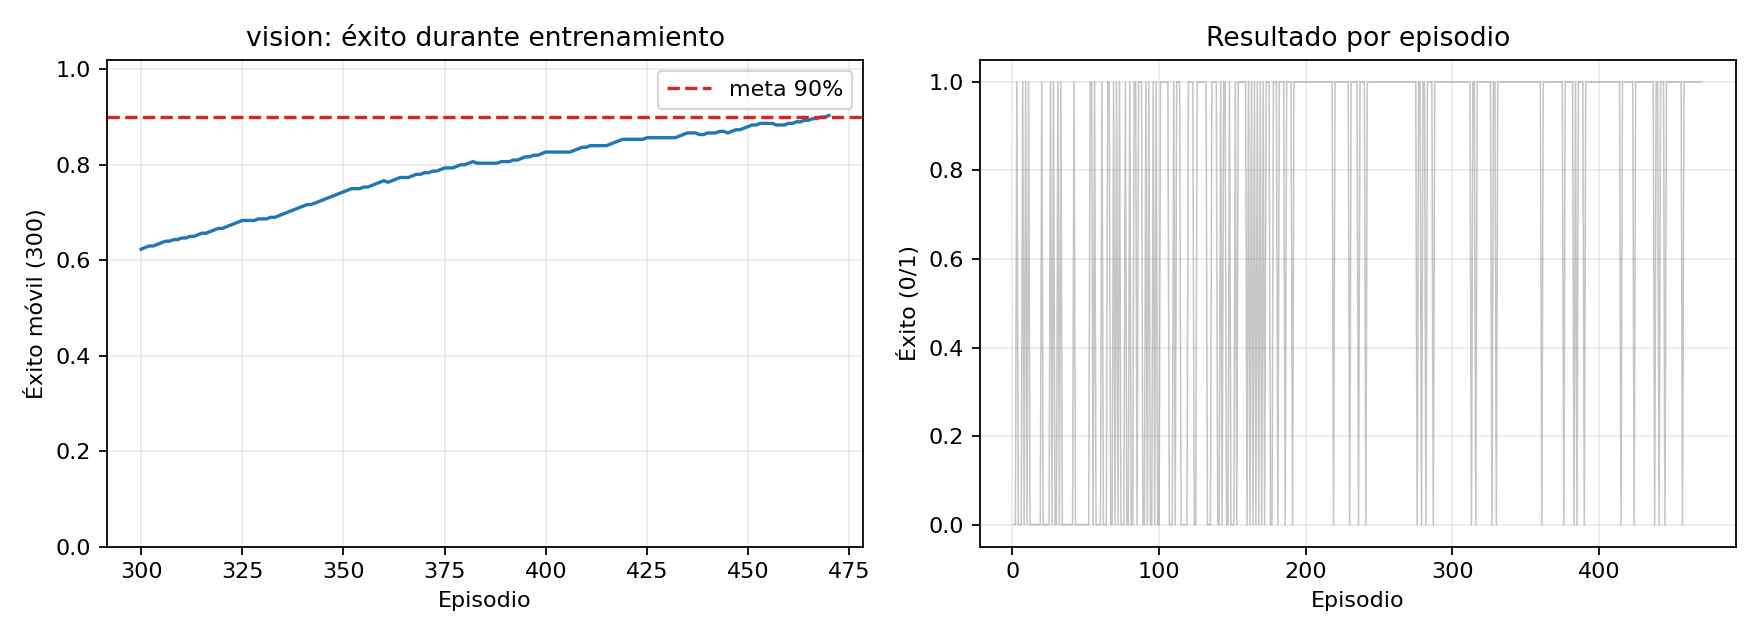
\includegraphics[width=\linewidth,height=0.14\textheight,keepaspectratio]{../../03_EVIDENCIAS/ENTRENAMIENTOS/COMPARATIVA_SEEDS_0_1_X0/runs/vision_rstdp_seed1_X0_0.9/success_curve.png}
\end{minipage}\par\smallskip
\clearpage
\noindent\textbf{Obst\'aculos | REINFORCE | semilla 0 | $X_0=0.1$}\\
{\scriptsize lote principal; episodios completados: 300; tasa de \'exito en la ventana final: 95.33\%; criterio alcanzado: s\'i.}\par
\noindent\begin{minipage}[t]{0.49\textwidth}
\centering
\textit{Crossbar $X$}\par
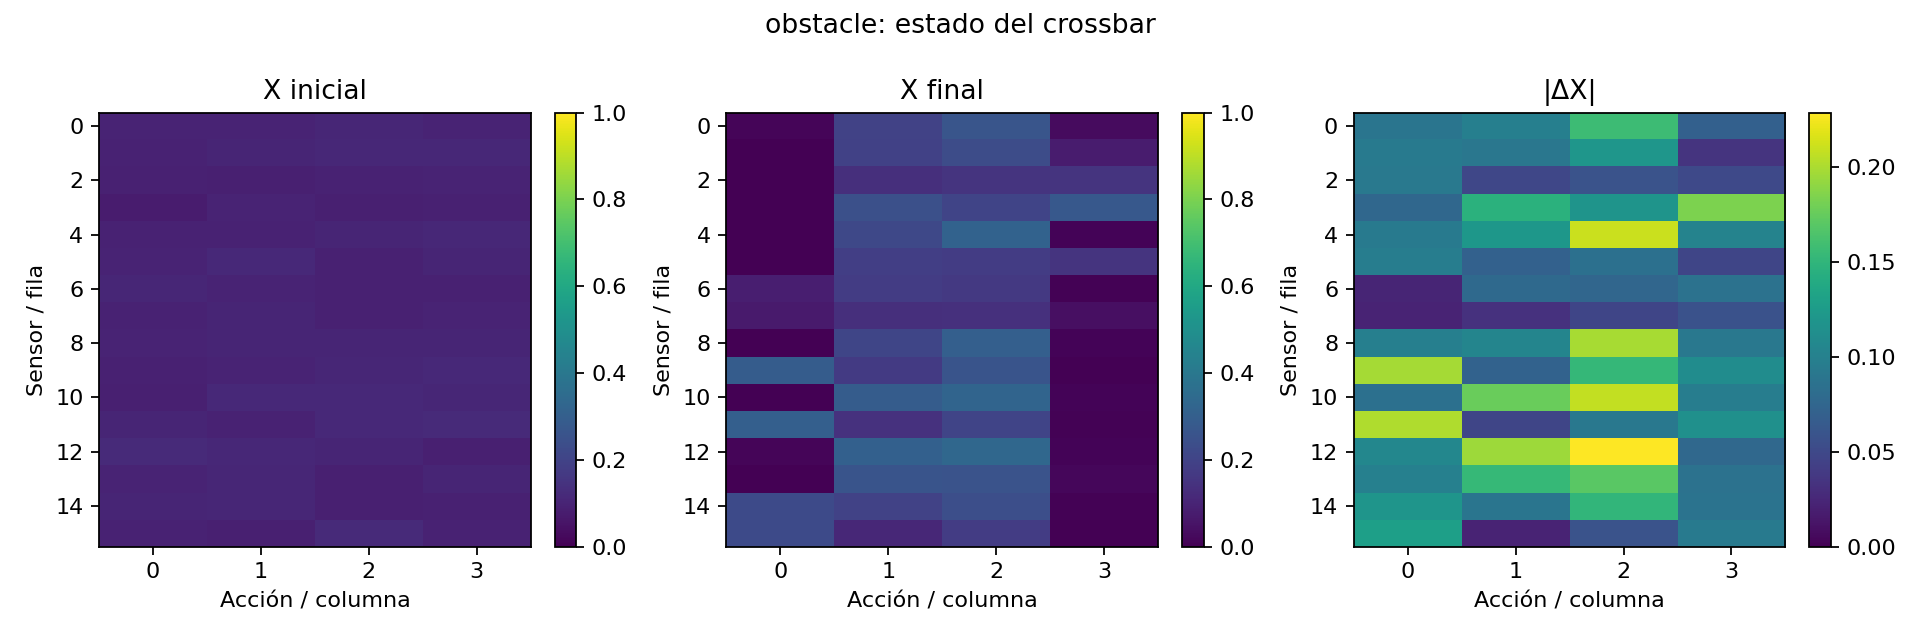
\includegraphics[width=\linewidth,height=0.14\textheight,keepaspectratio]{../../03_EVIDENCIAS/ENTRENAMIENTOS/COMPARATIVA_SEEDS_0_1_X0/runs/obstacle_reinforce_seed0_X0_0.1/crossbar.png}
\end{minipage}\hfill
\begin{minipage}[t]{0.49\textwidth}
\centering
\textit{Curva de \'exito}\par
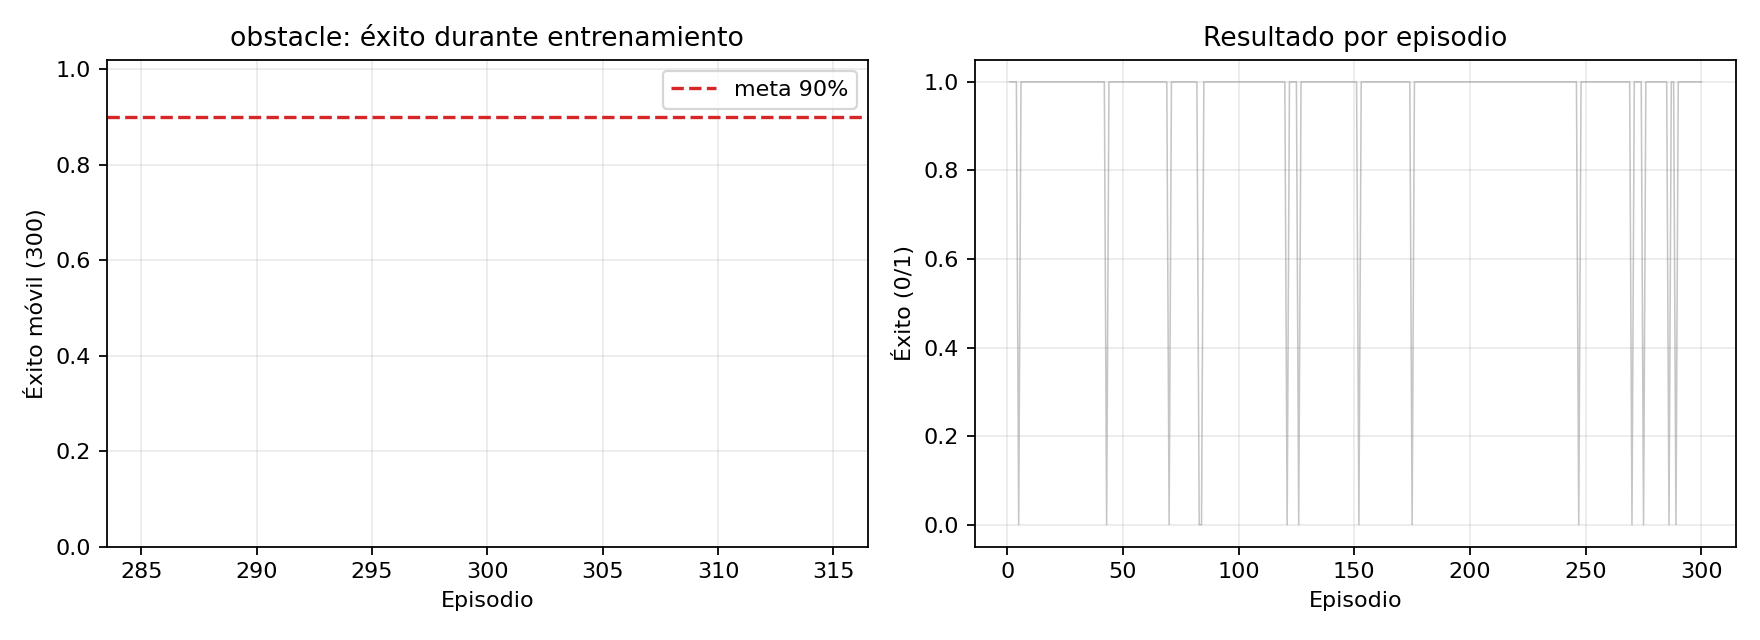
\includegraphics[width=\linewidth,height=0.14\textheight,keepaspectratio]{../../03_EVIDENCIAS/ENTRENAMIENTOS/COMPARATIVA_SEEDS_0_1_X0/runs/obstacle_reinforce_seed0_X0_0.1/success_curve.png}
\end{minipage}\par\smallskip
\noindent\textbf{Obst\'aculos | REINFORCE | semilla 0 | $X_0=0.9$}\\
{\scriptsize lote principal; episodios completados: 300; tasa de \'exito en la ventana final: 98.00\%; criterio alcanzado: s\'i.}\par
\noindent\begin{minipage}[t]{0.49\textwidth}
\centering
\textit{Crossbar $X$}\par
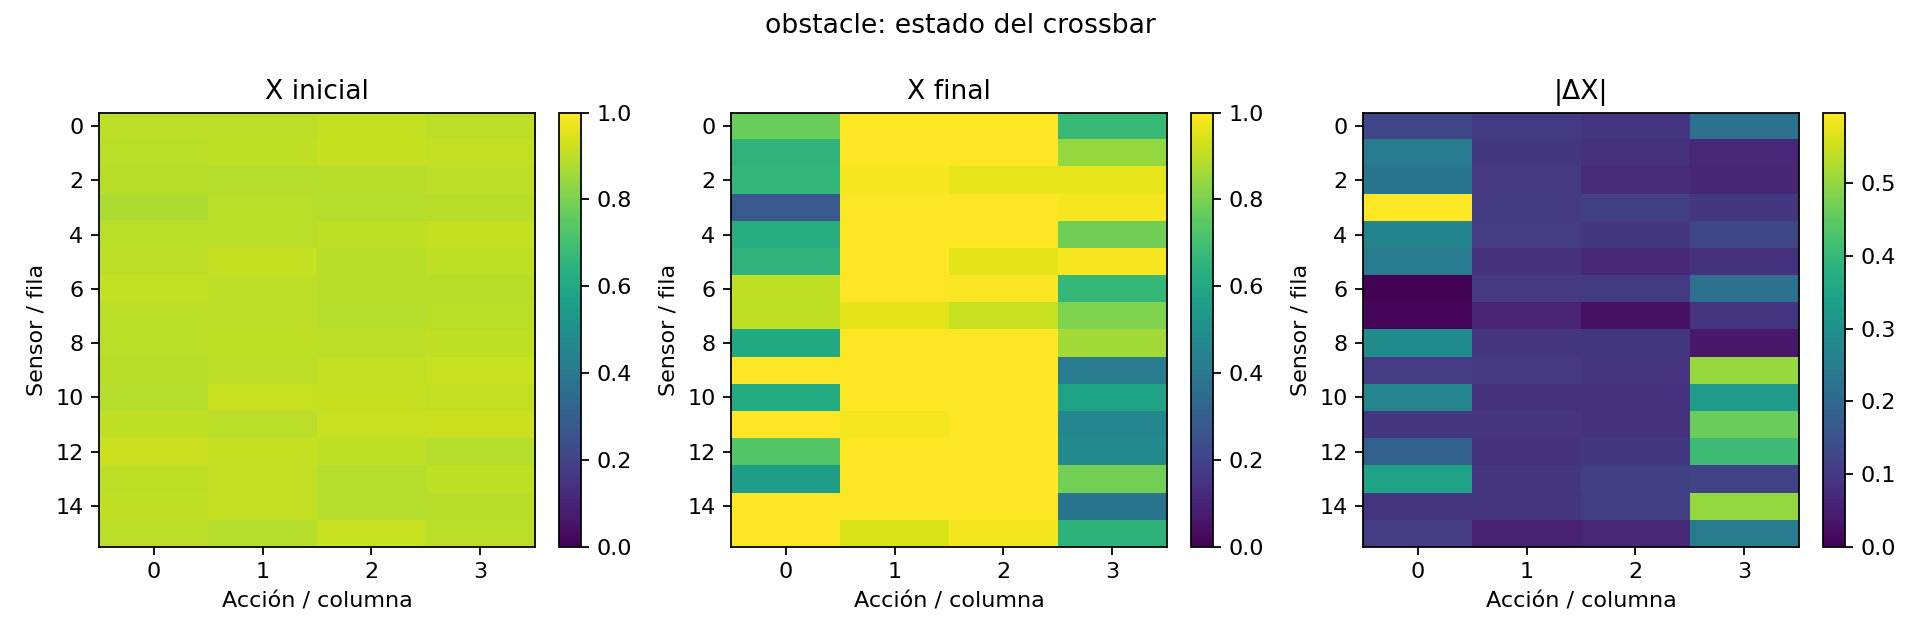
\includegraphics[width=\linewidth,height=0.14\textheight,keepaspectratio]{../../03_EVIDENCIAS/ENTRENAMIENTOS/COMPARATIVA_SEEDS_0_1_X0/runs/obstacle_reinforce_seed0_X0_0.9/crossbar.png}
\end{minipage}\hfill
\begin{minipage}[t]{0.49\textwidth}
\centering
\textit{Curva de \'exito}\par
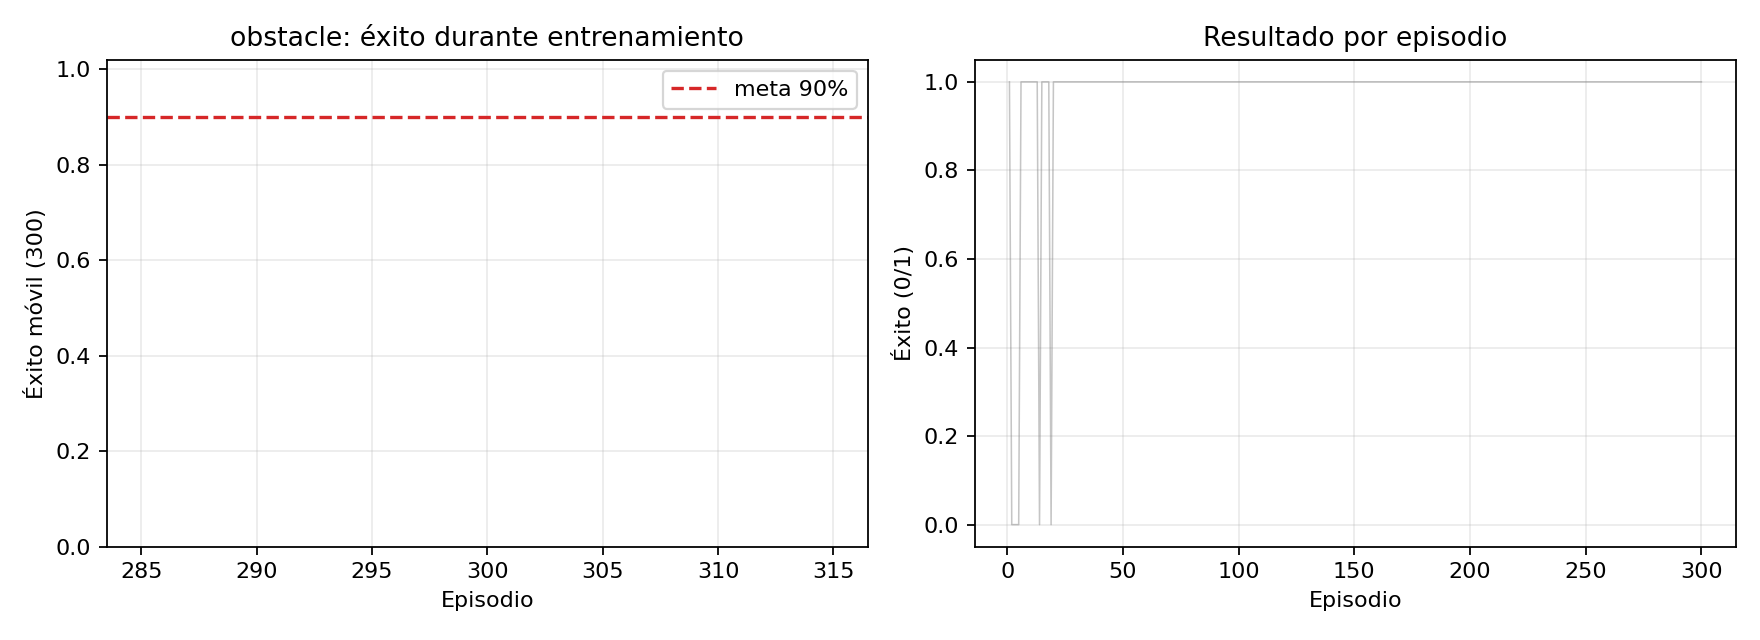
\includegraphics[width=\linewidth,height=0.14\textheight,keepaspectratio]{../../03_EVIDENCIAS/ENTRENAMIENTOS/COMPARATIVA_SEEDS_0_1_X0/runs/obstacle_reinforce_seed0_X0_0.9/success_curve.png}
\end{minipage}\par\smallskip
\noindent\textbf{Obst\'aculos | REINFORCE | semilla 1 | $X_0=0.1$}\\
{\scriptsize lote principal; episodios completados: 300; tasa de \'exito en la ventana final: 93.67\%; criterio alcanzado: s\'i.}\par
\noindent\begin{minipage}[t]{0.49\textwidth}
\centering
\textit{Crossbar $X$}\par
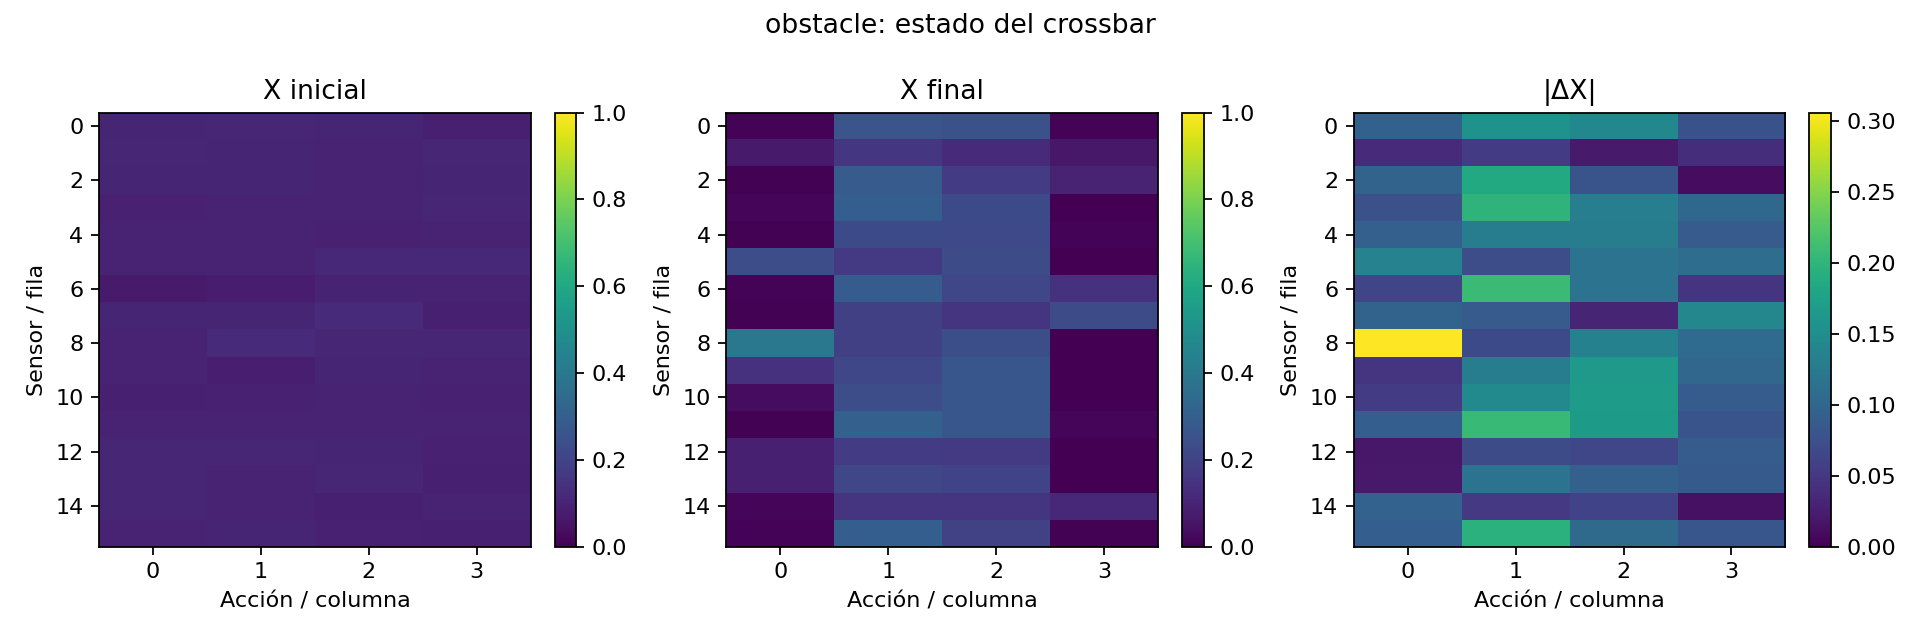
\includegraphics[width=\linewidth,height=0.14\textheight,keepaspectratio]{../../03_EVIDENCIAS/ENTRENAMIENTOS/COMPARATIVA_SEEDS_0_1_X0/runs/obstacle_reinforce_seed1_X0_0.1/crossbar.png}
\end{minipage}\hfill
\begin{minipage}[t]{0.49\textwidth}
\centering
\textit{Curva de \'exito}\par
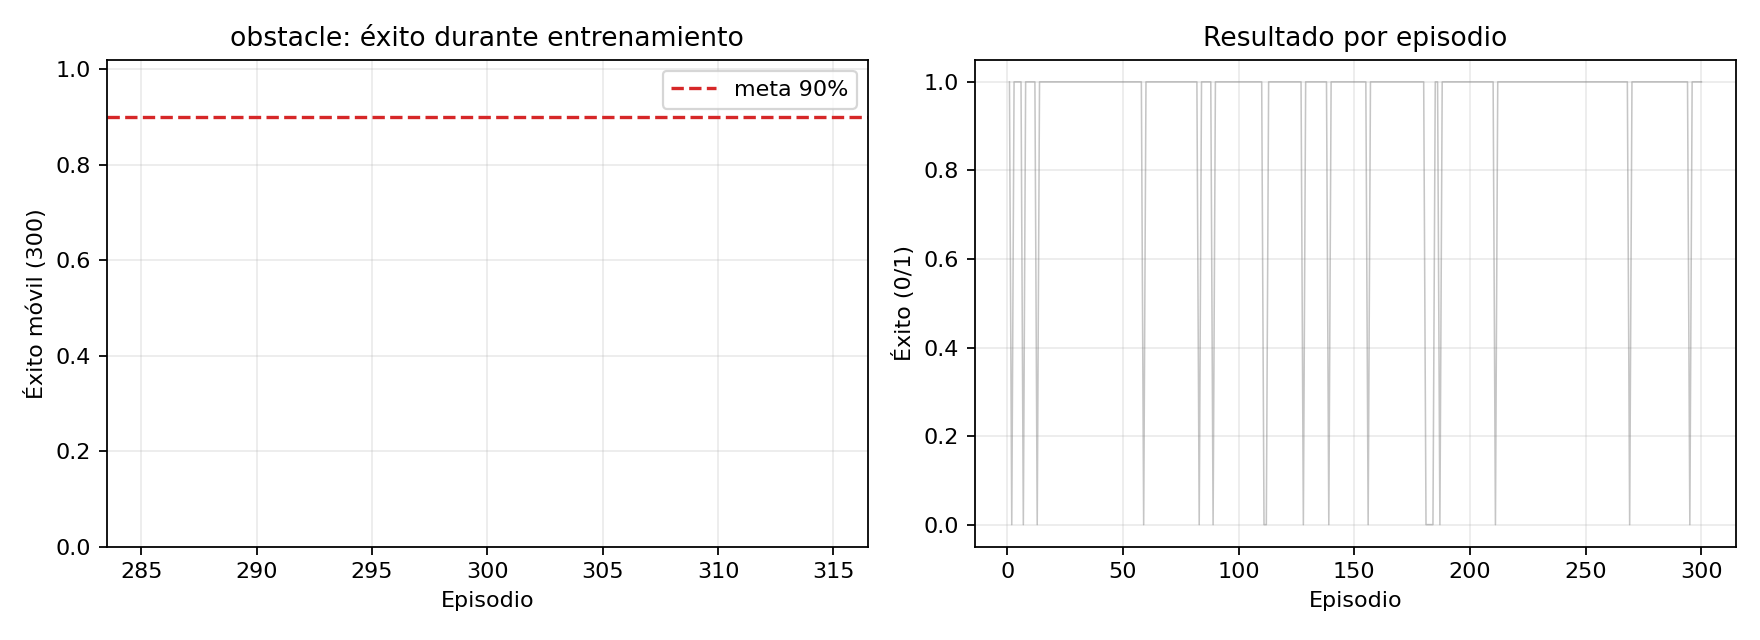
\includegraphics[width=\linewidth,height=0.14\textheight,keepaspectratio]{../../03_EVIDENCIAS/ENTRENAMIENTOS/COMPARATIVA_SEEDS_0_1_X0/runs/obstacle_reinforce_seed1_X0_0.1/success_curve.png}
\end{minipage}\par\smallskip
\noindent\textbf{Obst\'aculos | REINFORCE | semilla 1 | $X_0=0.9$}\\
{\scriptsize lote principal; episodios completados: 300; tasa de \'exito en la ventana final: 93.00\%; criterio alcanzado: s\'i.}\par
\noindent\begin{minipage}[t]{0.49\textwidth}
\centering
\textit{Crossbar $X$}\par
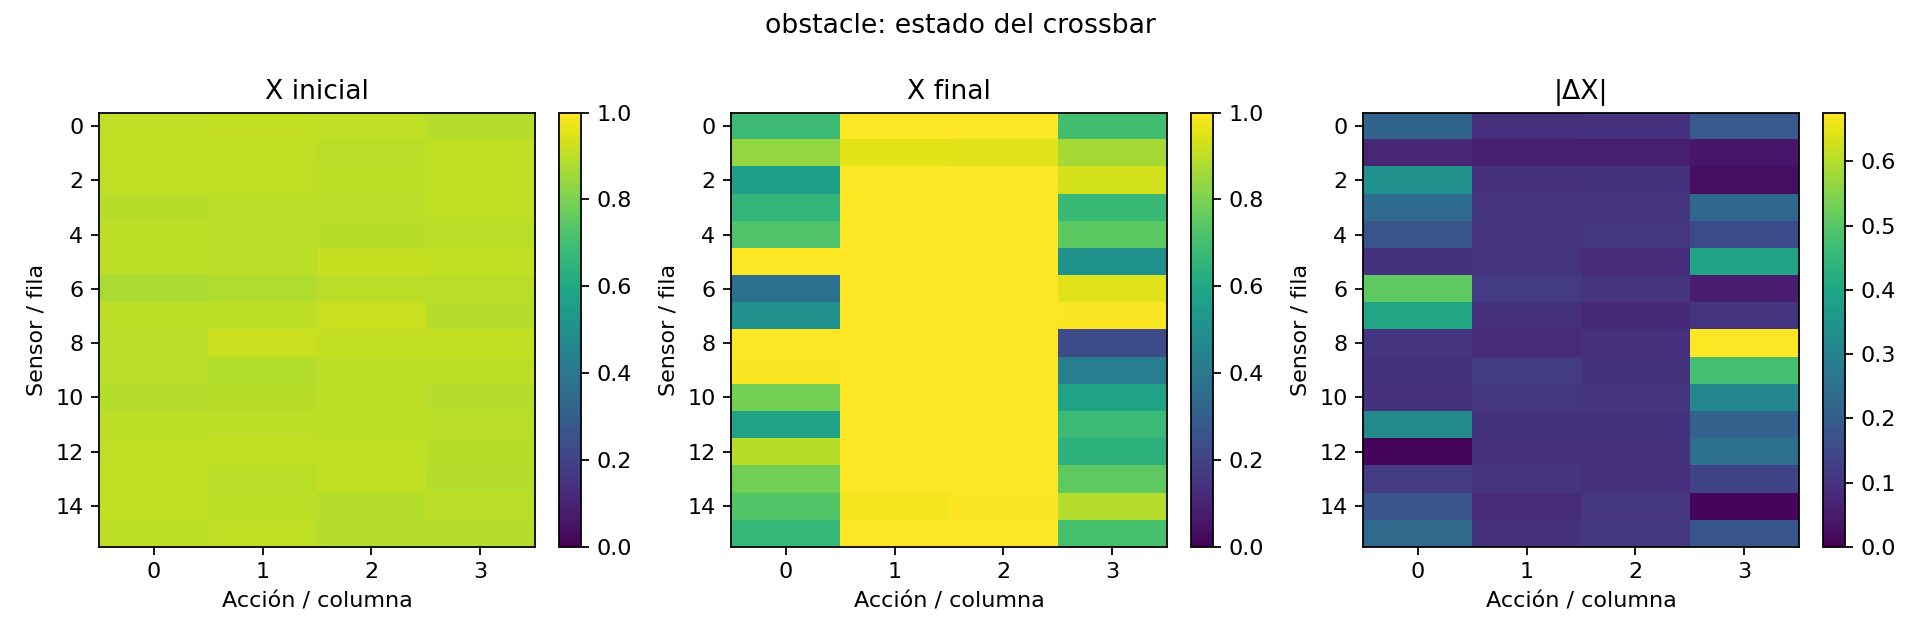
\includegraphics[width=\linewidth,height=0.14\textheight,keepaspectratio]{../../03_EVIDENCIAS/ENTRENAMIENTOS/COMPARATIVA_SEEDS_0_1_X0/runs/obstacle_reinforce_seed1_X0_0.9/crossbar.png}
\end{minipage}\hfill
\begin{minipage}[t]{0.49\textwidth}
\centering
\textit{Curva de \'exito}\par
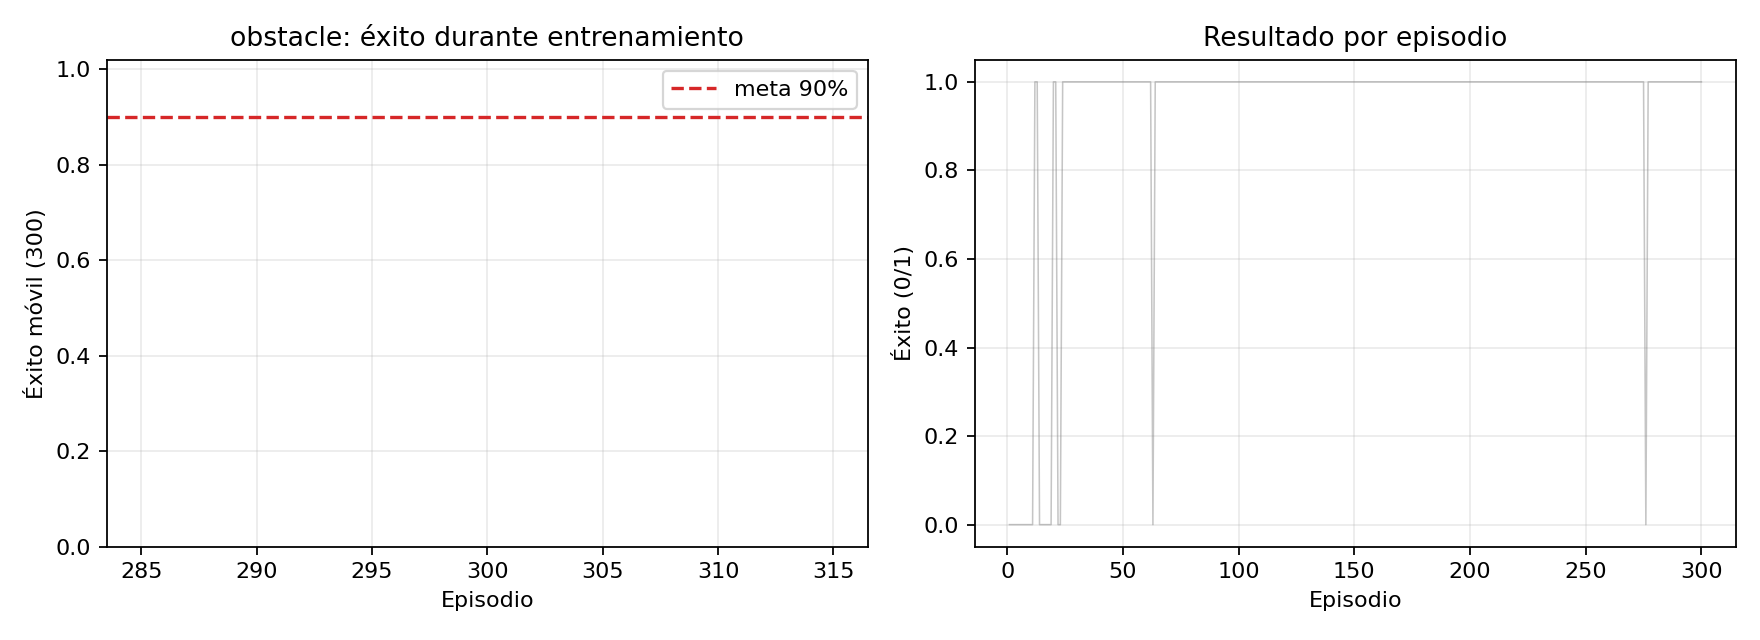
\includegraphics[width=\linewidth,height=0.14\textheight,keepaspectratio]{../../03_EVIDENCIAS/ENTRENAMIENTOS/COMPARATIVA_SEEDS_0_1_X0/runs/obstacle_reinforce_seed1_X0_0.9/success_curve.png}
\end{minipage}\par\smallskip
\clearpage
\noindent\textbf{Obst\'aculos | R-STDP | semilla 0 | $X_0=0.1$}\\
{\scriptsize lote principal; episodios completados: 300; tasa de \'exito en la ventana final: 99.67\%; criterio alcanzado: s\'i.}\par
\noindent\begin{minipage}[t]{0.49\textwidth}
\centering
\textit{Crossbar $X$}\par
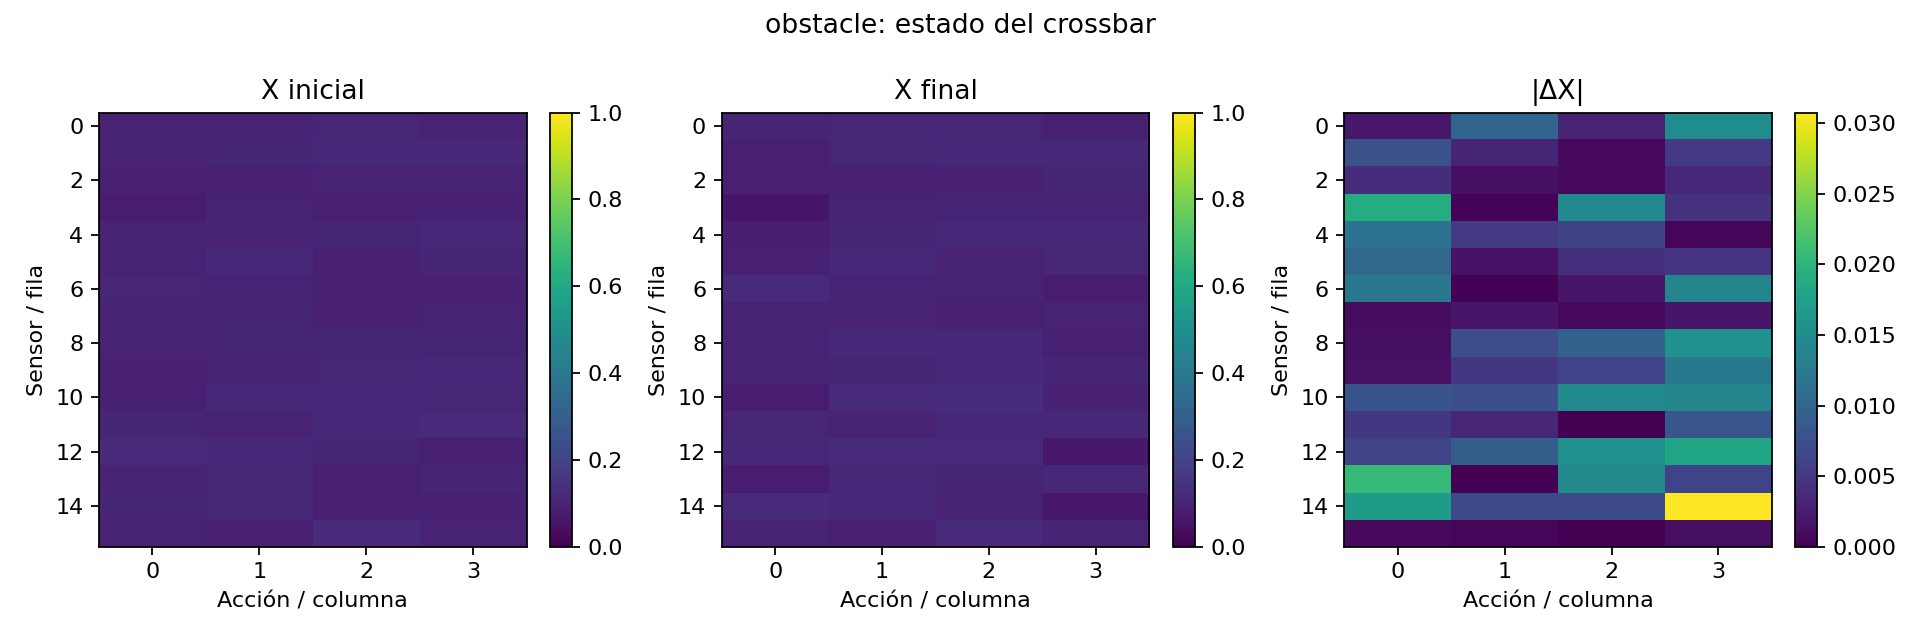
\includegraphics[width=\linewidth,height=0.14\textheight,keepaspectratio]{../../03_EVIDENCIAS/ENTRENAMIENTOS/COMPARATIVA_SEEDS_0_1_X0/runs/obstacle_rstdp_seed0_X0_0.1/crossbar.png}
\end{minipage}\hfill
\begin{minipage}[t]{0.49\textwidth}
\centering
\textit{Curva de \'exito}\par
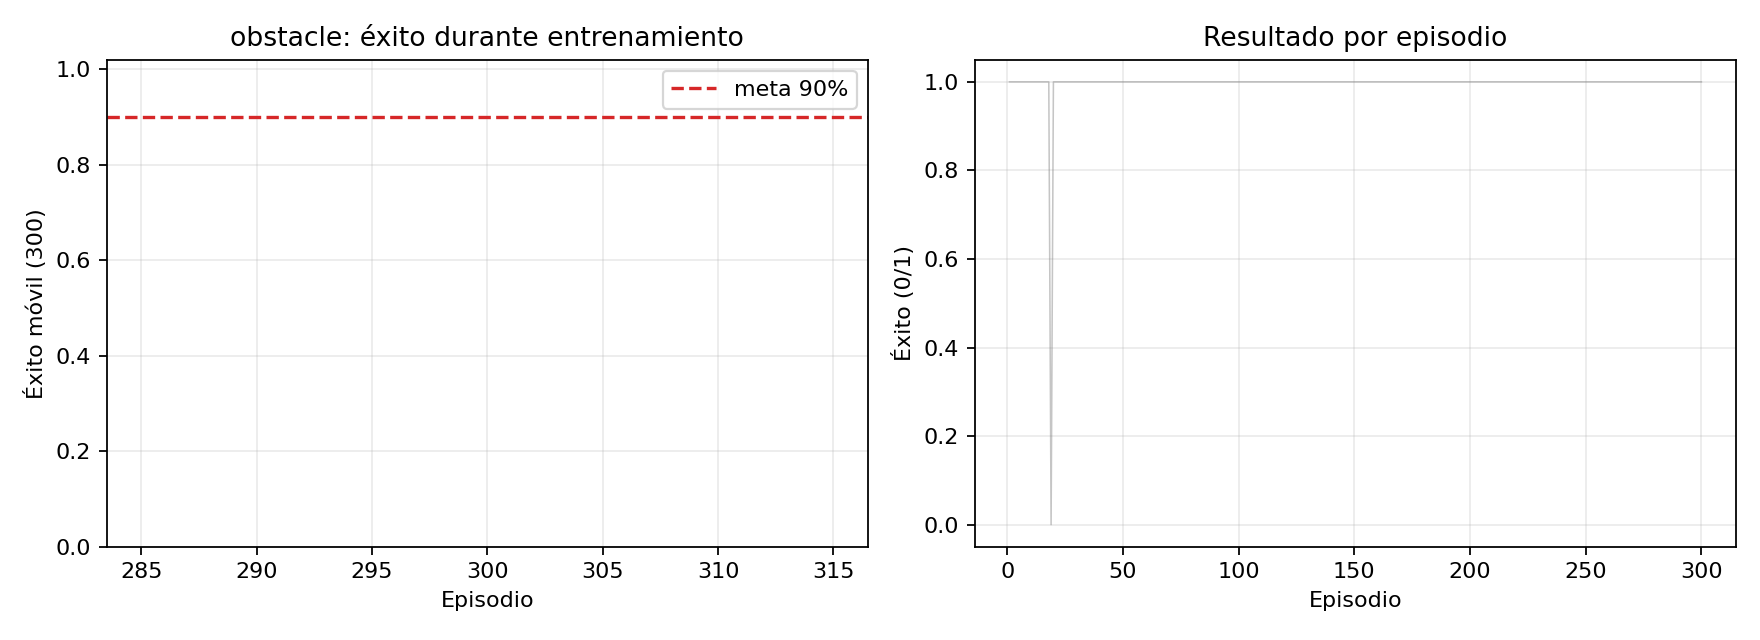
\includegraphics[width=\linewidth,height=0.14\textheight,keepaspectratio]{../../03_EVIDENCIAS/ENTRENAMIENTOS/COMPARATIVA_SEEDS_0_1_X0/runs/obstacle_rstdp_seed0_X0_0.1/success_curve.png}
\end{minipage}\par\smallskip
\noindent\textbf{Obst\'aculos | R-STDP | semilla 0 | $X_0=0.9$}\\
{\scriptsize lote principal; episodios completados: 318; tasa de \'exito en la ventana final: 90.33\%; criterio alcanzado: s\'i.}\par
\noindent\begin{minipage}[t]{0.49\textwidth}
\centering
\textit{Crossbar $X$}\par
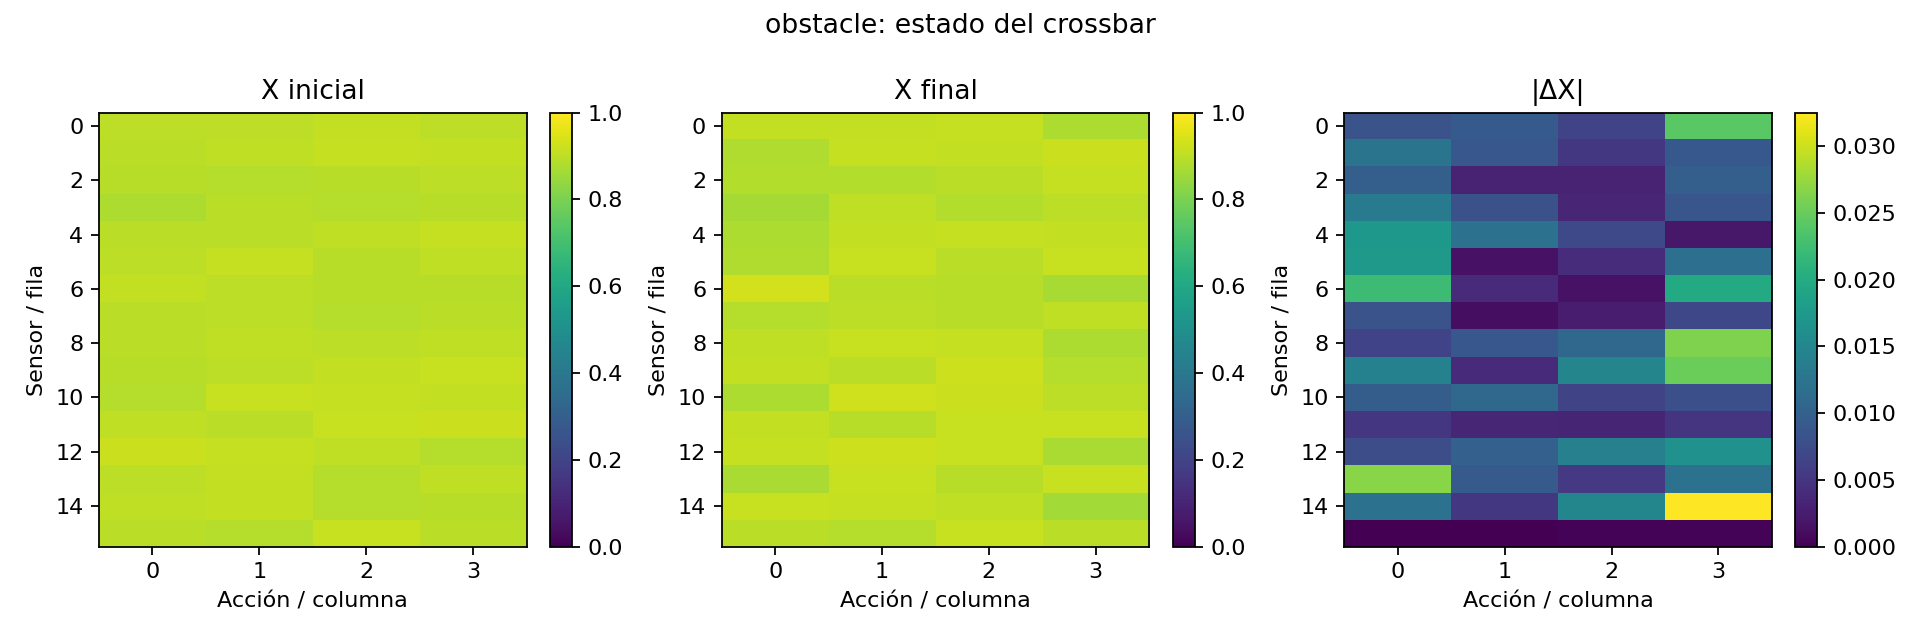
\includegraphics[width=\linewidth,height=0.14\textheight,keepaspectratio]{../../03_EVIDENCIAS/ENTRENAMIENTOS/COMPARATIVA_SEEDS_0_1_X0/runs/obstacle_rstdp_seed0_X0_0.9/crossbar.png}
\end{minipage}\hfill
\begin{minipage}[t]{0.49\textwidth}
\centering
\textit{Curva de \'exito}\par
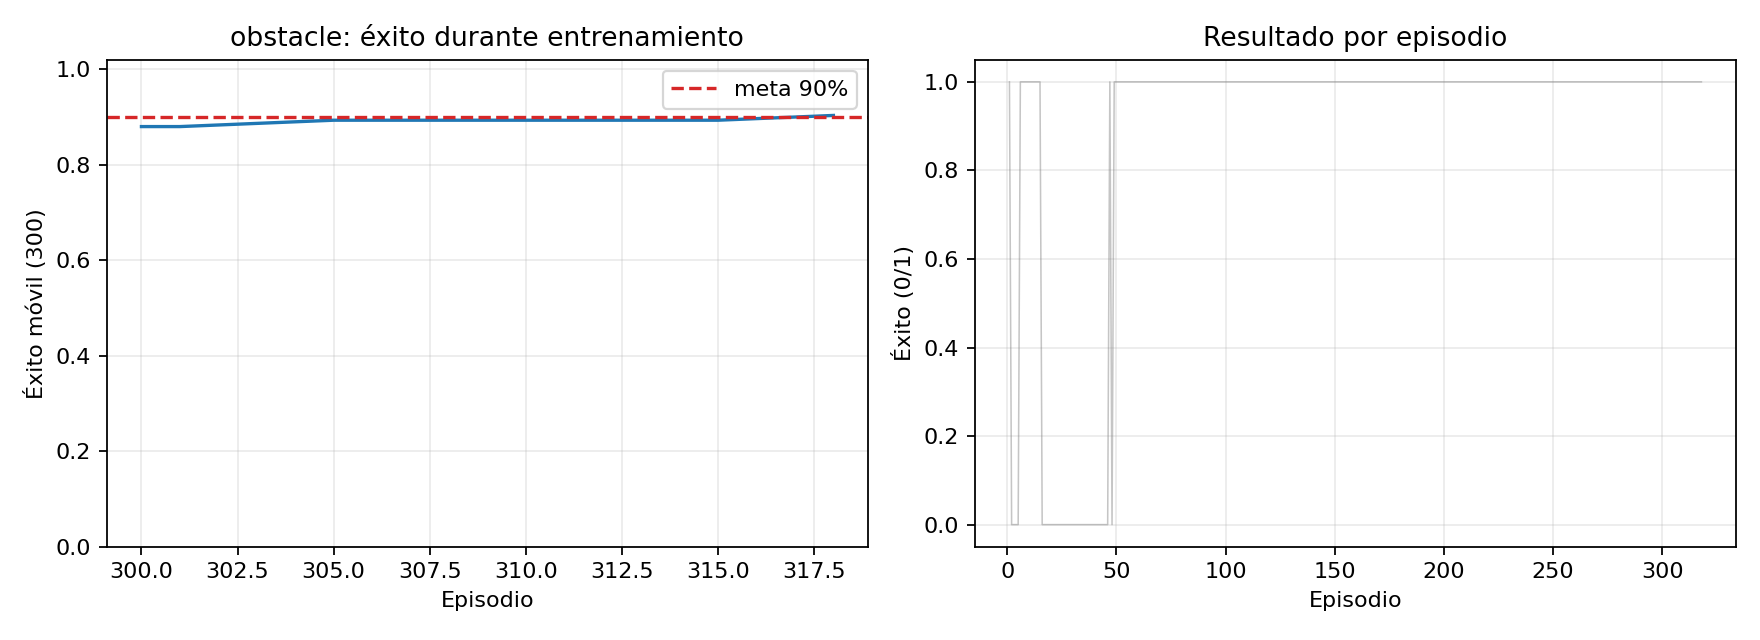
\includegraphics[width=\linewidth,height=0.14\textheight,keepaspectratio]{../../03_EVIDENCIAS/ENTRENAMIENTOS/COMPARATIVA_SEEDS_0_1_X0/runs/obstacle_rstdp_seed0_X0_0.9/success_curve.png}
\end{minipage}\par\smallskip
\noindent\textbf{Obst\'aculos | R-STDP | semilla 1 | $X_0=0.1$}\\
{\scriptsize lote principal; episodios completados: 336; tasa de \'exito en la ventana final: 90.33\%; criterio alcanzado: s\'i.}\par
\noindent\begin{minipage}[t]{0.49\textwidth}
\centering
\textit{Crossbar $X$}\par
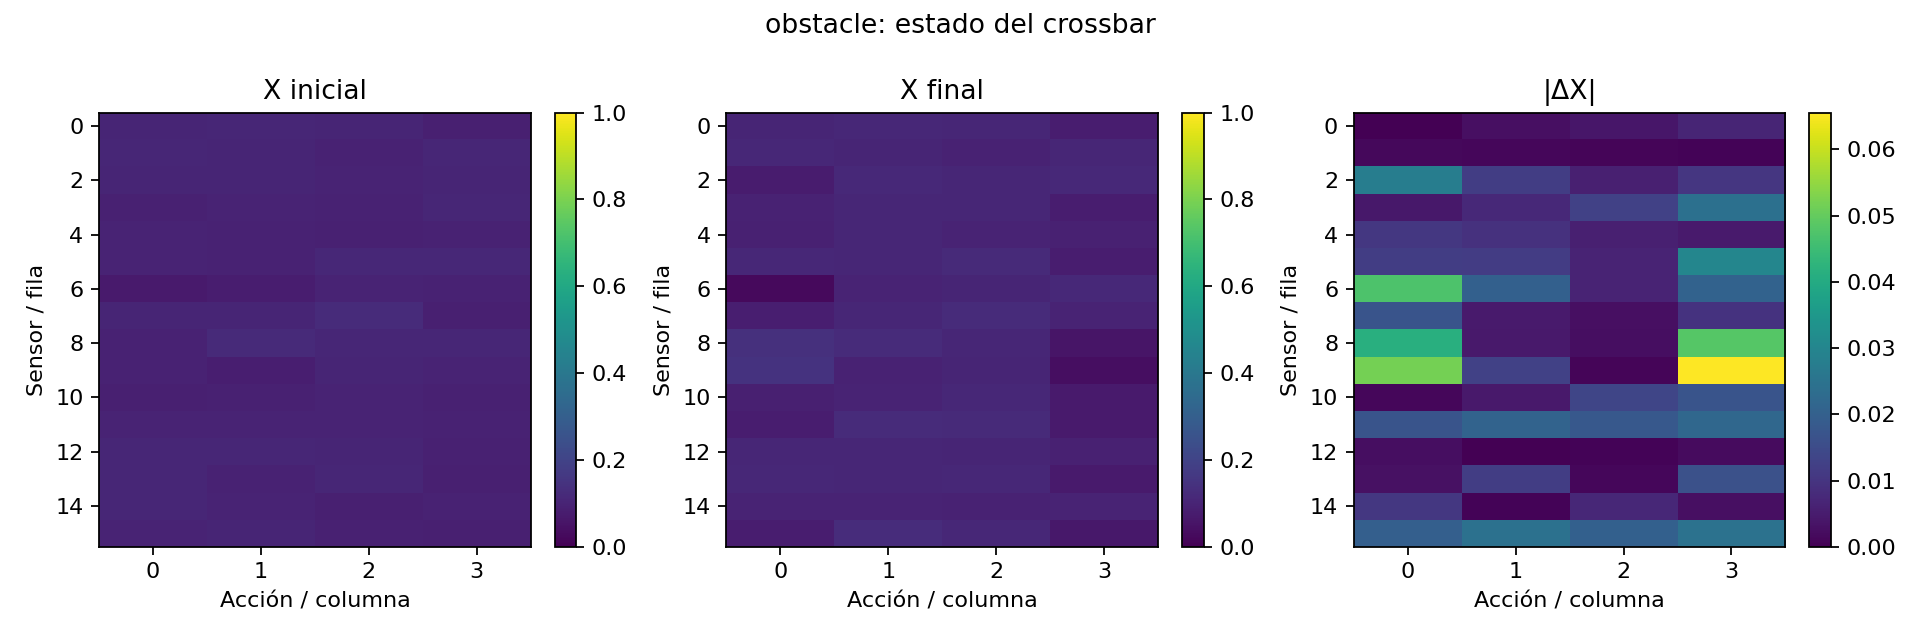
\includegraphics[width=\linewidth,height=0.14\textheight,keepaspectratio]{../../03_EVIDENCIAS/ENTRENAMIENTOS/COMPARATIVA_SEEDS_0_1_X0/runs/obstacle_rstdp_seed1_X0_0.1/crossbar.png}
\end{minipage}\hfill
\begin{minipage}[t]{0.49\textwidth}
\centering
\textit{Curva de \'exito}\par
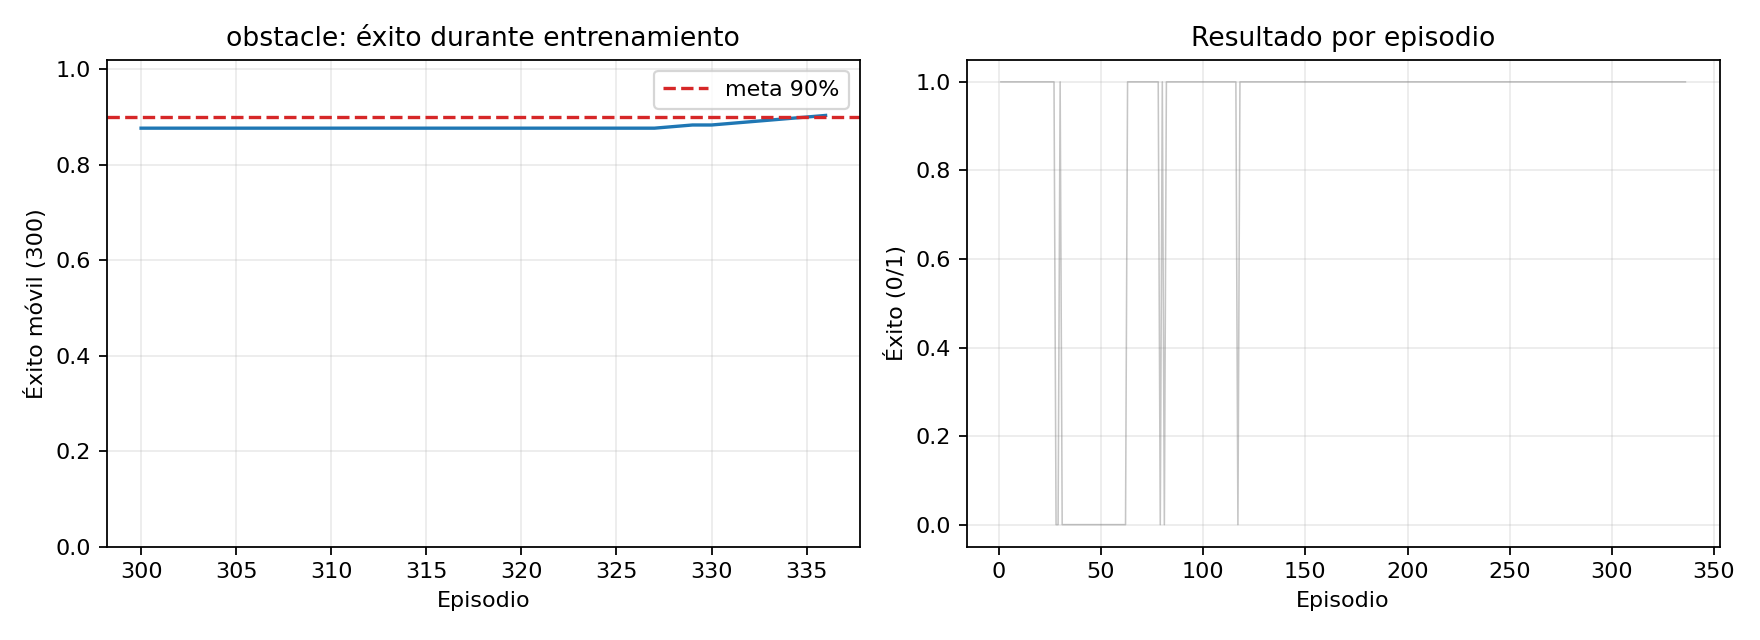
\includegraphics[width=\linewidth,height=0.14\textheight,keepaspectratio]{../../03_EVIDENCIAS/ENTRENAMIENTOS/COMPARATIVA_SEEDS_0_1_X0/runs/obstacle_rstdp_seed1_X0_0.1/success_curve.png}
\end{minipage}\par\smallskip
\noindent\textbf{Obst\'aculos | R-STDP | semilla 1 | $X_0=0.9$}\\
{\scriptsize lote principal; episodios completados: 300; tasa de \'exito en la ventana final: 99.67\%; criterio alcanzado: s\'i.}\par
\noindent\begin{minipage}[t]{0.49\textwidth}
\centering
\textit{Crossbar $X$}\par
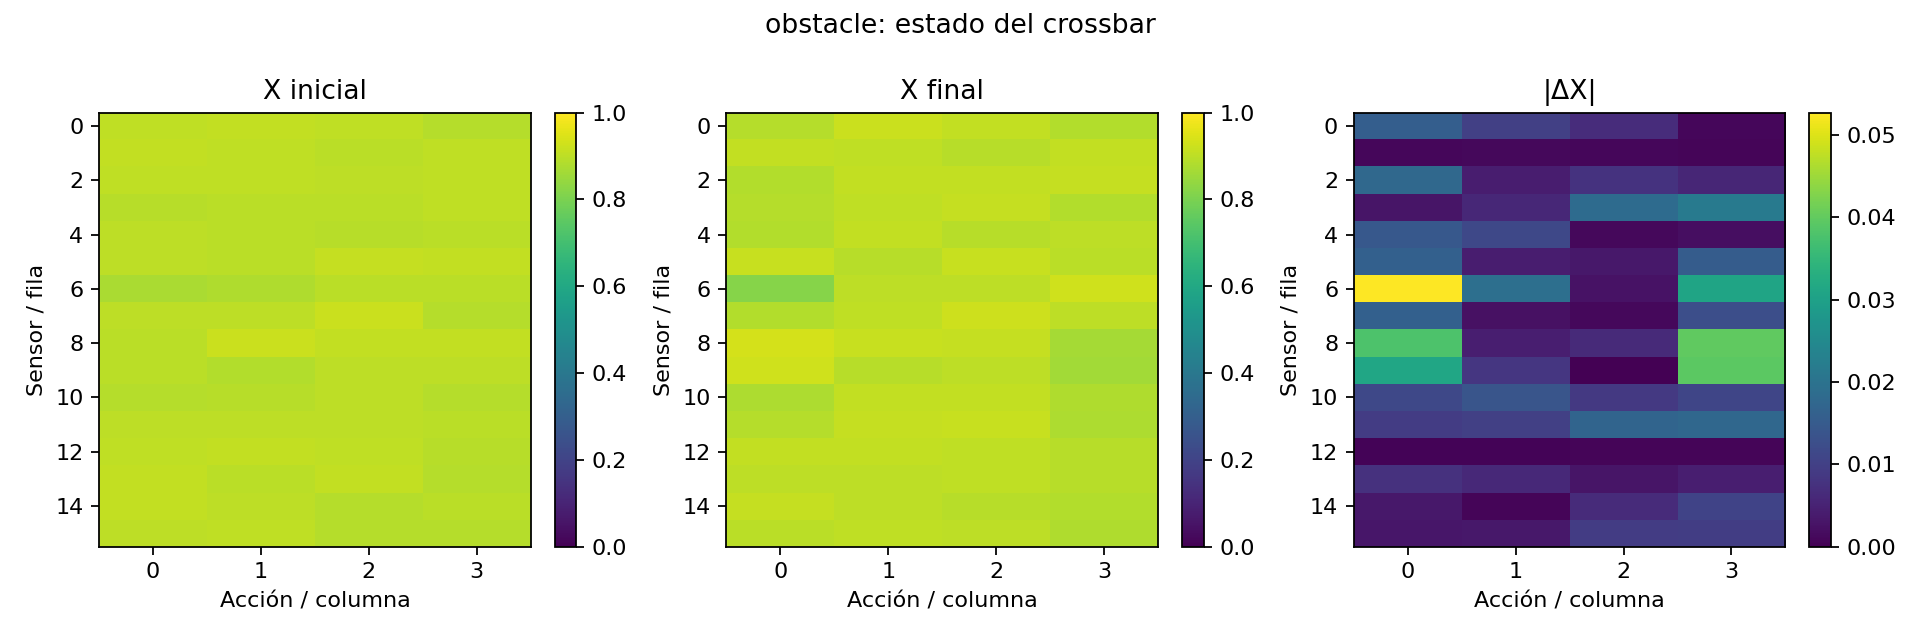
\includegraphics[width=\linewidth,height=0.14\textheight,keepaspectratio]{../../03_EVIDENCIAS/ENTRENAMIENTOS/COMPARATIVA_SEEDS_0_1_X0/runs/obstacle_rstdp_seed1_X0_0.9/crossbar.png}
\end{minipage}\hfill
\begin{minipage}[t]{0.49\textwidth}
\centering
\textit{Curva de \'exito}\par
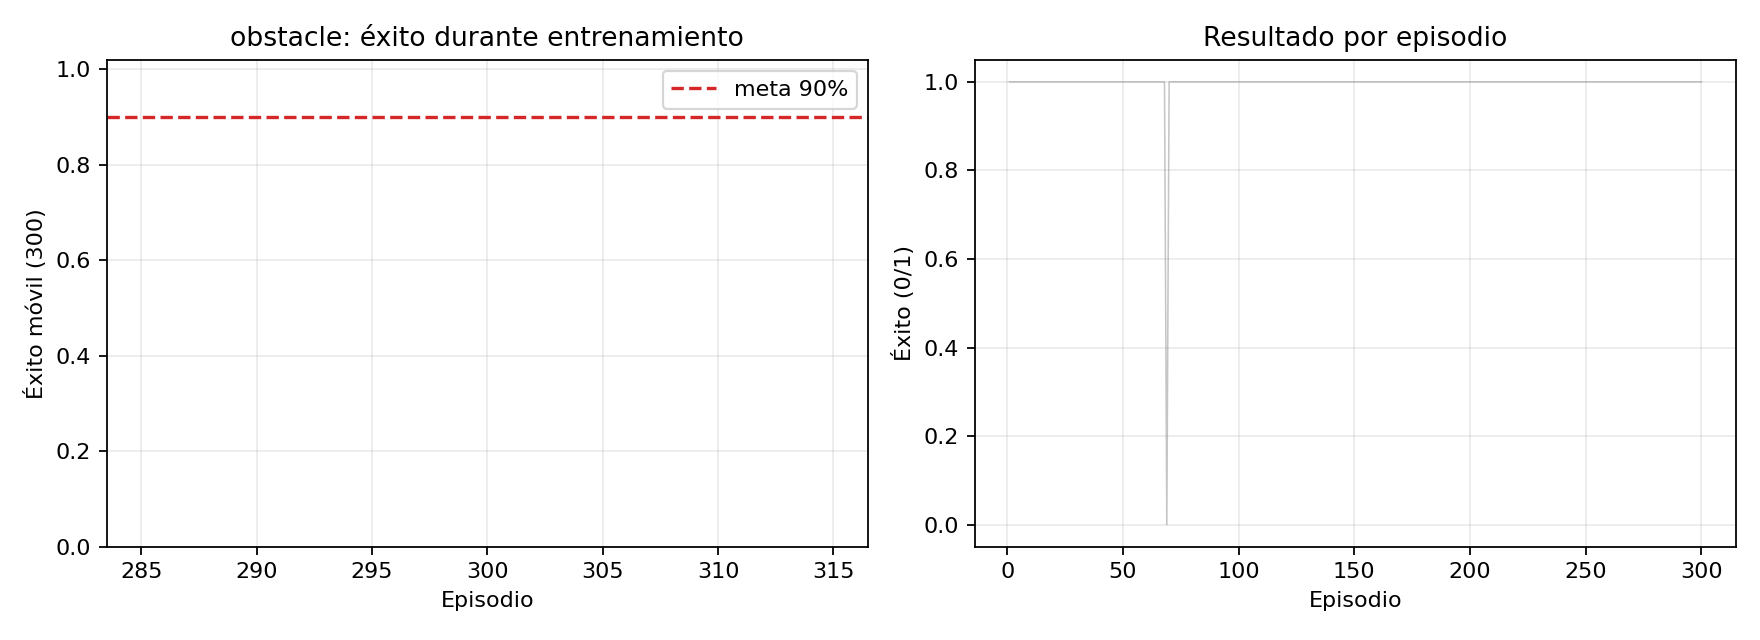
\includegraphics[width=\linewidth,height=0.14\textheight,keepaspectratio]{../../03_EVIDENCIAS/ENTRENAMIENTOS/COMPARATIVA_SEEDS_0_1_X0/runs/obstacle_rstdp_seed1_X0_0.9/success_curve.png}
\end{minipage}\par\smallskip
\clearpage
\noindent\textbf{Car | R-STDP | semilla 0 | $X_0=0.1$}\\
{\scriptsize lote principal; episodios completados: 3775; tasa de \'exito en la ventana final: 90.33\%; criterio alcanzado: s\'i.}\par
\noindent\begin{minipage}[t]{0.49\textwidth}
\centering
\textit{Crossbar $X$}\par
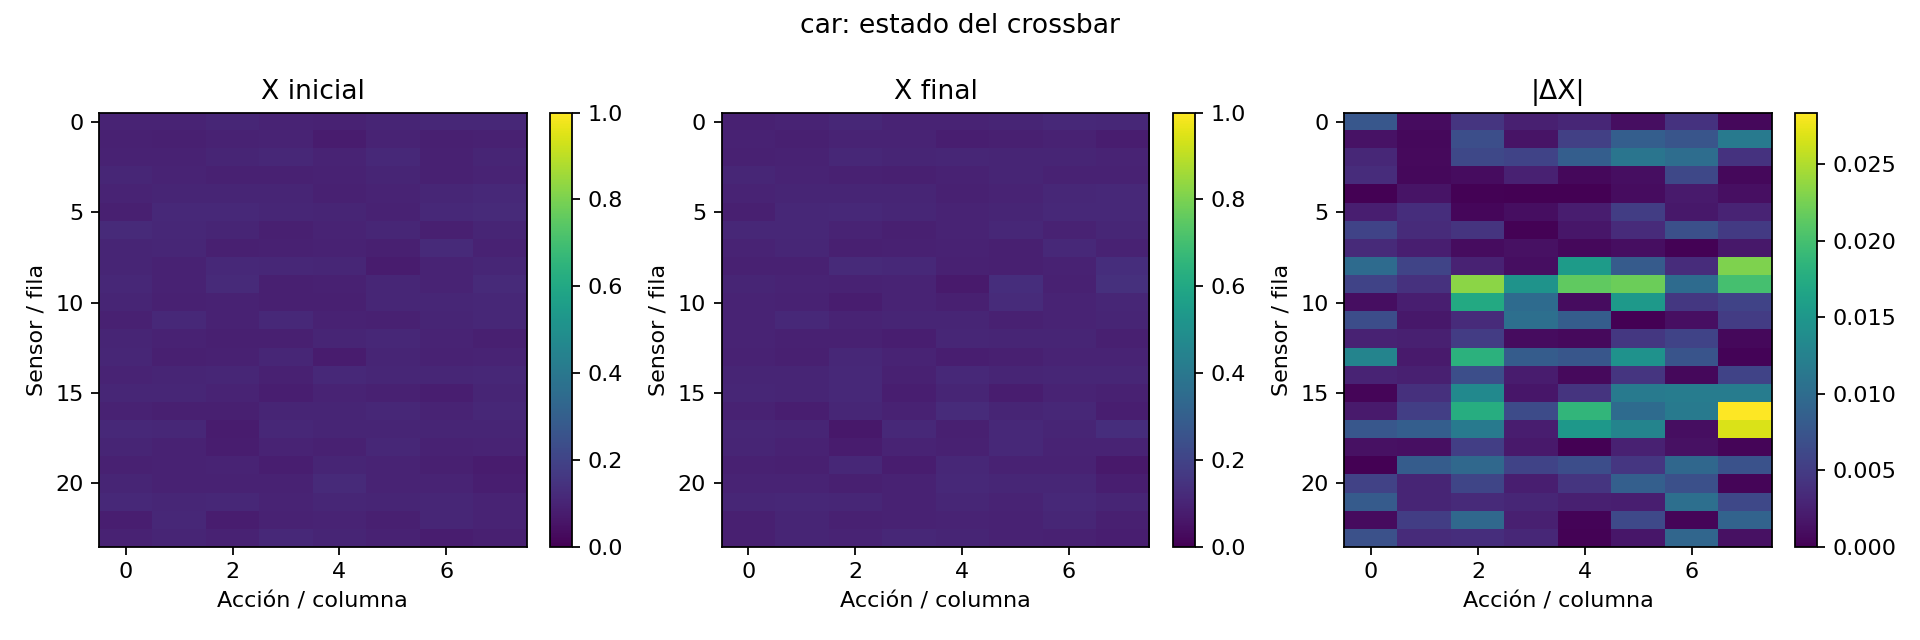
\includegraphics[width=\linewidth,height=0.14\textheight,keepaspectratio]{../../03_EVIDENCIAS/ENTRENAMIENTOS/COMPARATIVA_SEEDS_0_1_X0/runs/car_rstdp_seed0_X0_0.1/crossbar.png}
\end{minipage}\hfill
\begin{minipage}[t]{0.49\textwidth}
\centering
\textit{Curva de \'exito}\par
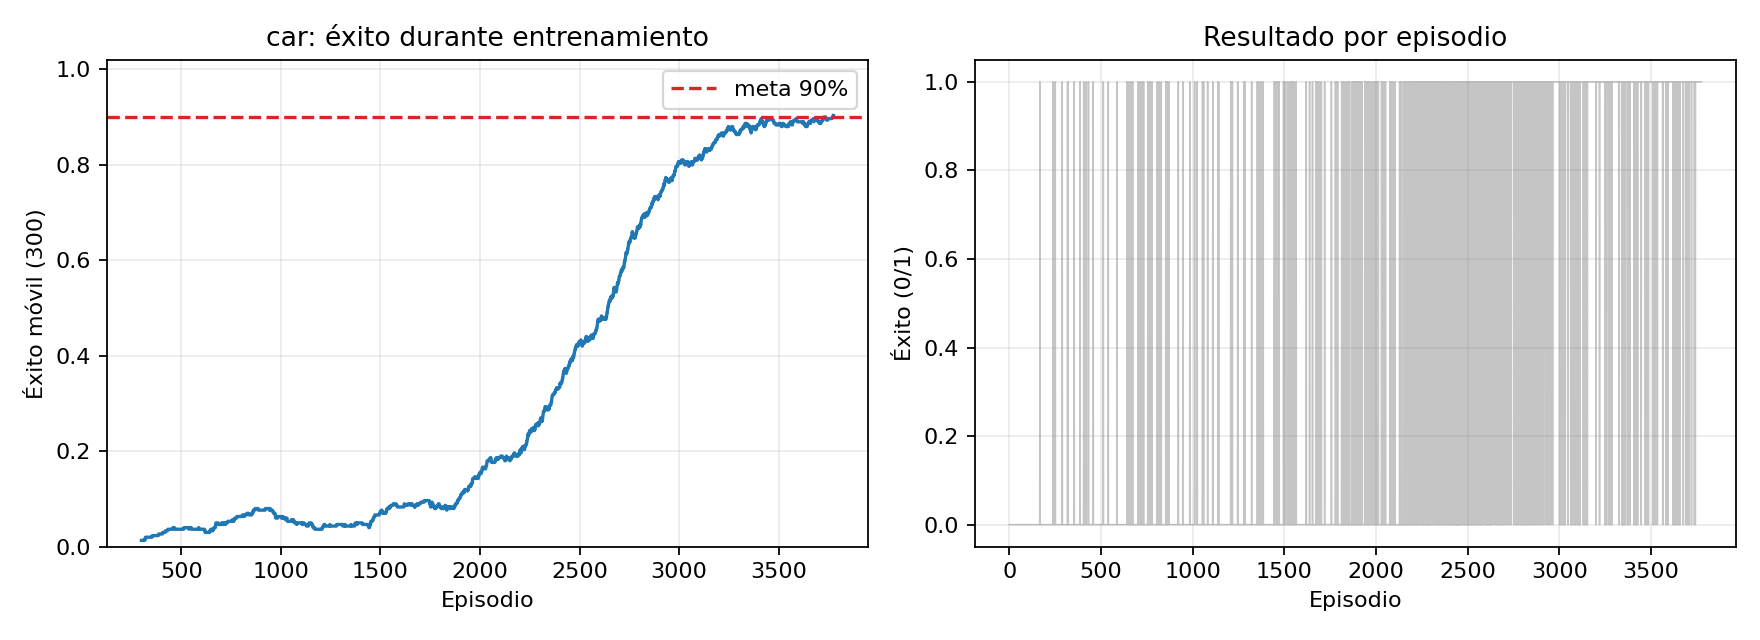
\includegraphics[width=\linewidth,height=0.14\textheight,keepaspectratio]{../../03_EVIDENCIAS/ENTRENAMIENTOS/COMPARATIVA_SEEDS_0_1_X0/runs/car_rstdp_seed0_X0_0.1/success_curve.png}
\end{minipage}\par\smallskip
\noindent\textbf{Car | R-STDP | semilla 0 | $X_0=0.9$}\\
{\scriptsize lote principal; episodios completados: 10000; tasa de \'exito en la ventana final: 11.00\%; criterio alcanzado: no.}\par
\noindent\begin{minipage}[t]{0.49\textwidth}
\centering
\textit{Crossbar $X$}\par
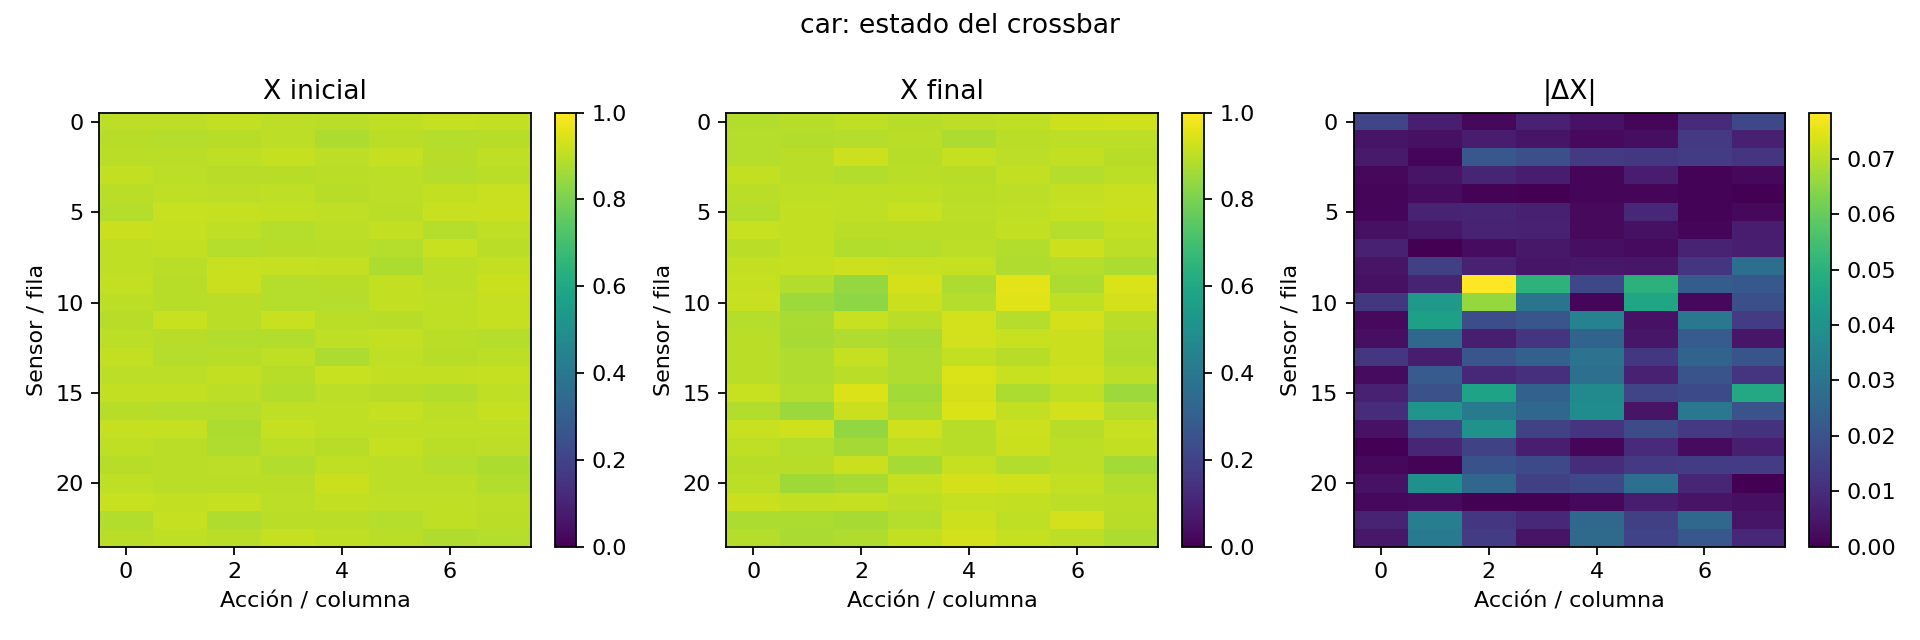
\includegraphics[width=\linewidth,height=0.14\textheight,keepaspectratio]{../../03_EVIDENCIAS/ENTRENAMIENTOS/COMPARATIVA_SEEDS_0_1_X0/runs/car_rstdp_seed0_X0_0.9/crossbar.png}
\end{minipage}\hfill
\begin{minipage}[t]{0.49\textwidth}
\centering
\textit{Curva de \'exito}\par
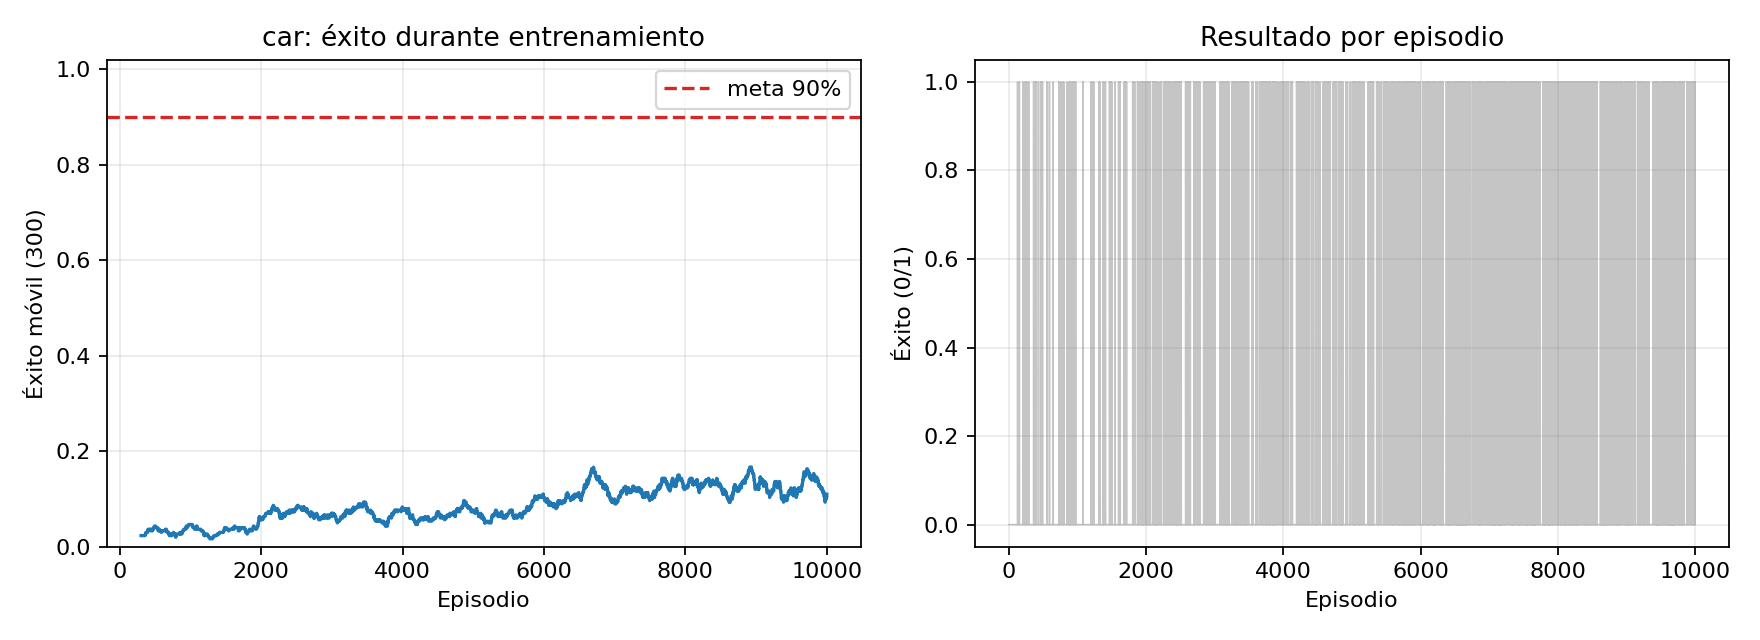
\includegraphics[width=\linewidth,height=0.14\textheight,keepaspectratio]{../../03_EVIDENCIAS/ENTRENAMIENTOS/COMPARATIVA_SEEDS_0_1_X0/runs/car_rstdp_seed0_X0_0.9/success_curve.png}
\end{minipage}\par\smallskip
\noindent\textbf{Car | R-STDP | semilla 1 | $X_0=0.1$}\\
{\scriptsize lote principal; episodios completados: 10000; tasa de \'exito en la ventana final: 42.67\%; criterio alcanzado: no.}\par
\noindent\begin{minipage}[t]{0.49\textwidth}
\centering
\textit{Crossbar $X$}\par
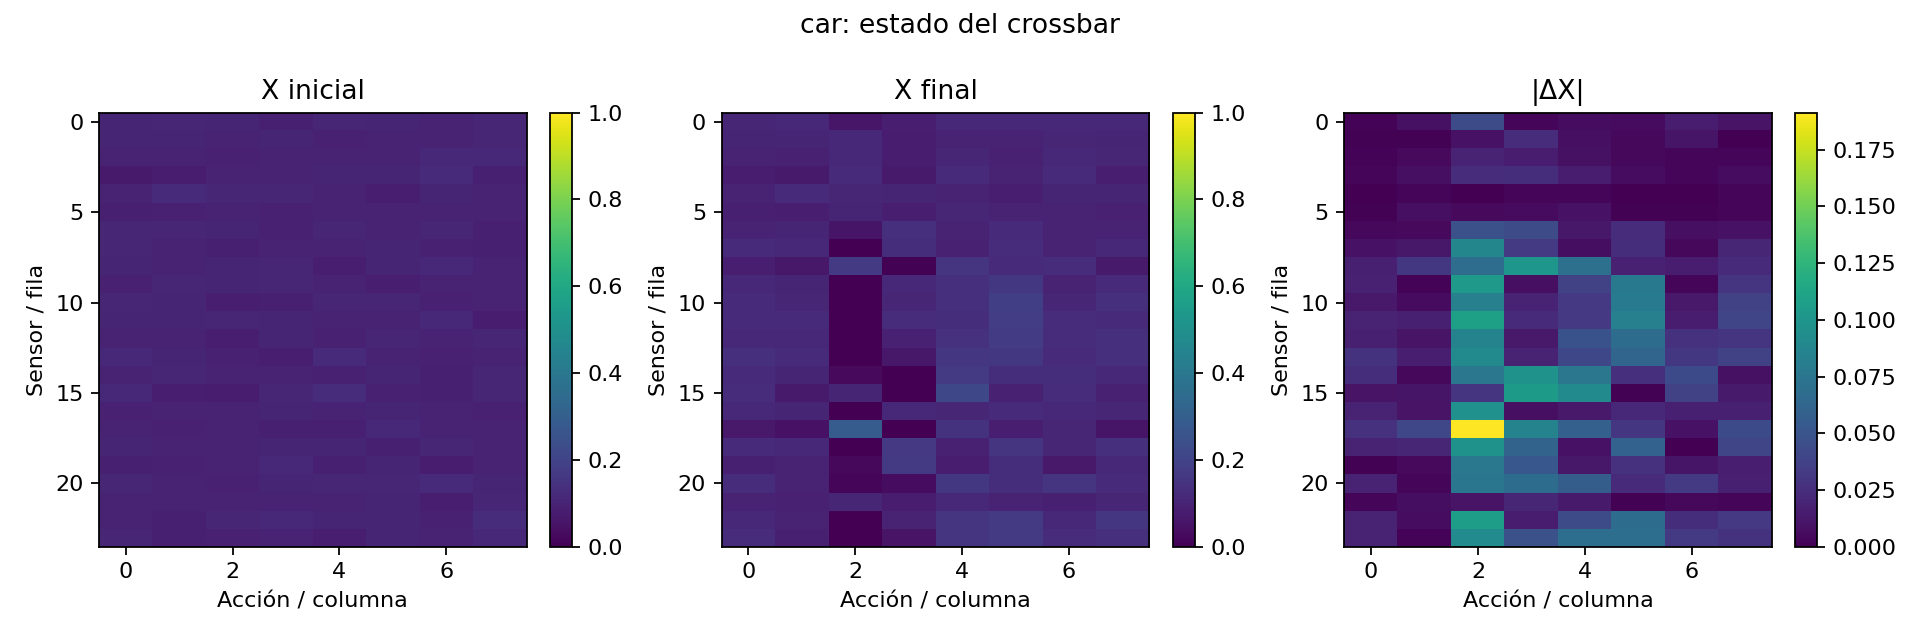
\includegraphics[width=\linewidth,height=0.14\textheight,keepaspectratio]{../../03_EVIDENCIAS/ENTRENAMIENTOS/COMPARATIVA_SEEDS_0_1_X0/runs/car_rstdp_seed1_X0_0.1/crossbar.png}
\end{minipage}\hfill
\begin{minipage}[t]{0.49\textwidth}
\centering
\textit{Curva de \'exito}\par
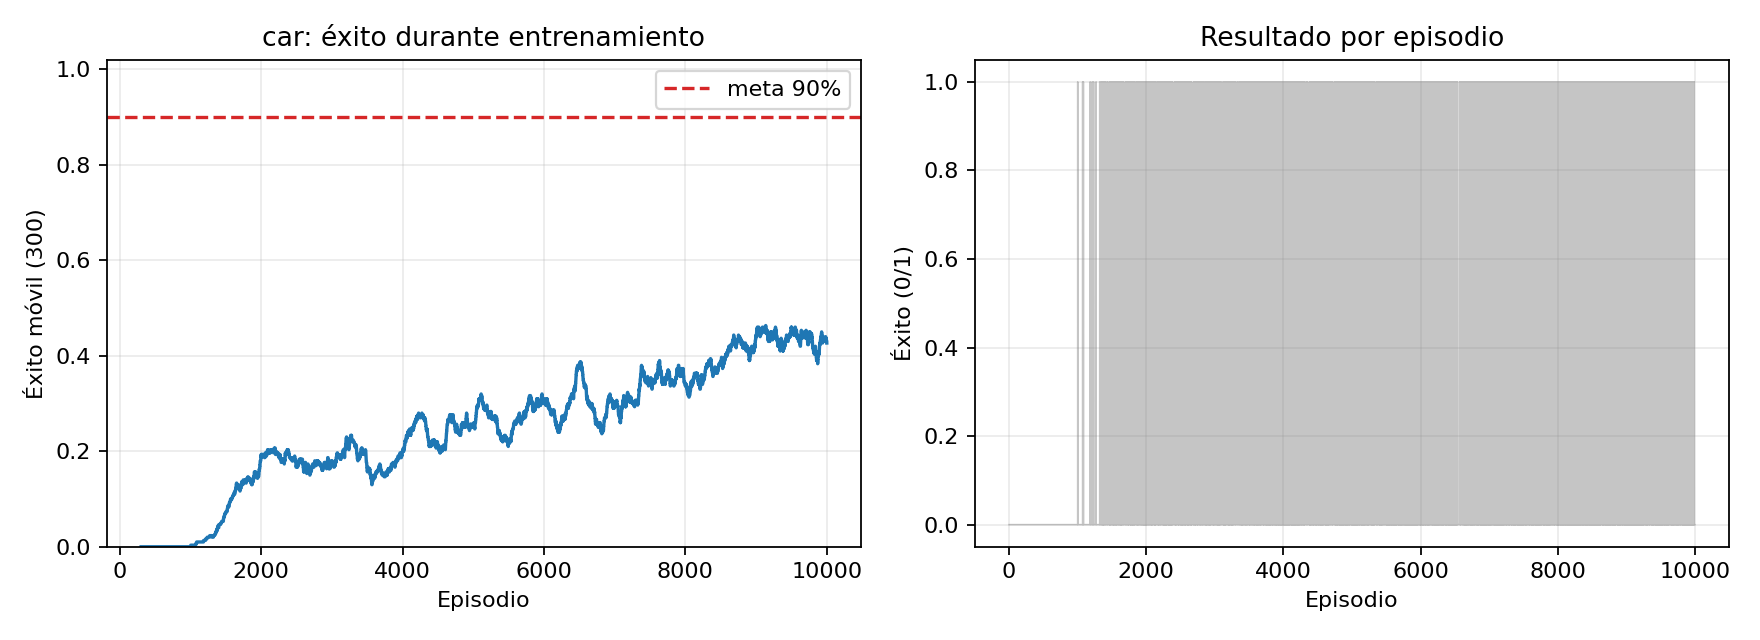
\includegraphics[width=\linewidth,height=0.14\textheight,keepaspectratio]{../../03_EVIDENCIAS/ENTRENAMIENTOS/COMPARATIVA_SEEDS_0_1_X0/runs/car_rstdp_seed1_X0_0.1/success_curve.png}
\end{minipage}\par\smallskip
\noindent\textbf{Car | R-STDP | semilla 1 | $X_0=0.9$}\\
{\scriptsize lote principal; episodios completados: 10000; tasa de \'exito en la ventana final: 25.33\%; criterio alcanzado: no.}\par
\noindent\begin{minipage}[t]{0.49\textwidth}
\centering
\textit{Crossbar $X$}\par
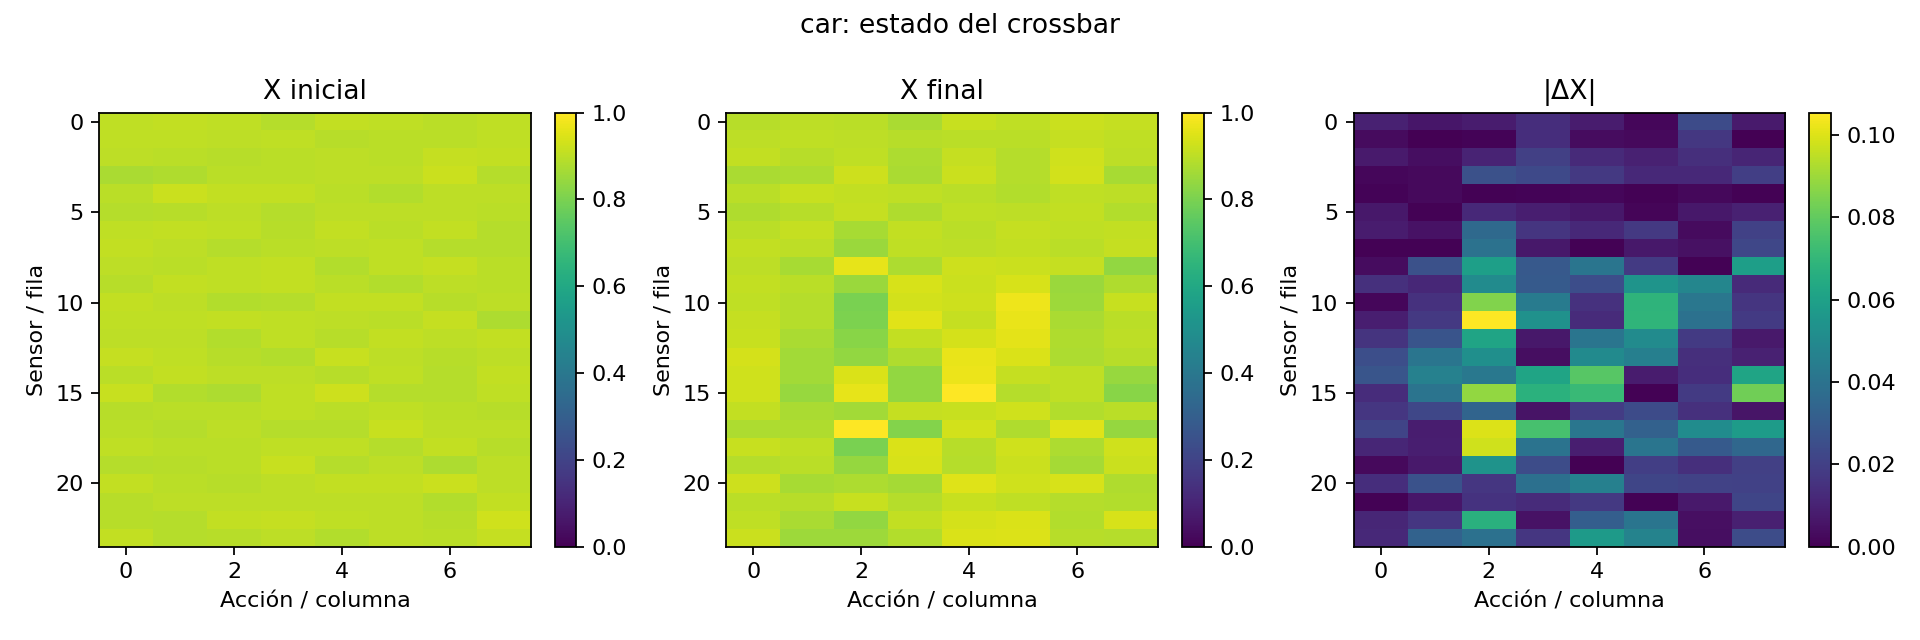
\includegraphics[width=\linewidth,height=0.14\textheight,keepaspectratio]{../../03_EVIDENCIAS/ENTRENAMIENTOS/COMPARATIVA_SEEDS_0_1_X0/runs/car_rstdp_seed1_X0_0.9/crossbar.png}
\end{minipage}\hfill
\begin{minipage}[t]{0.49\textwidth}
\centering
\textit{Curva de \'exito}\par
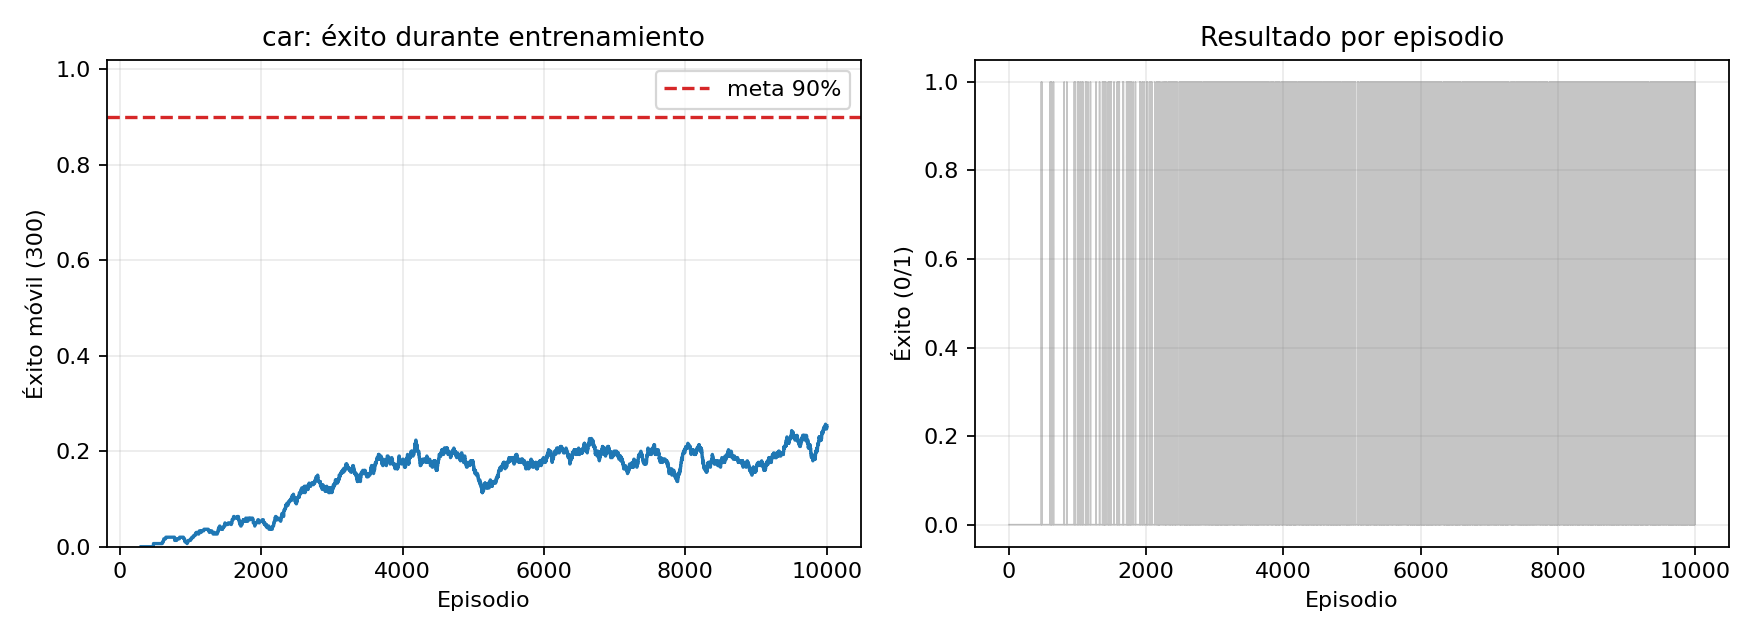
\includegraphics[width=\linewidth,height=0.14\textheight,keepaspectratio]{../../03_EVIDENCIAS/ENTRENAMIENTOS/COMPARATIVA_SEEDS_0_1_X0/runs/car_rstdp_seed1_X0_0.9/success_curve.png}
\end{minipage}\par\smallskip
\clearpage
\noindent\textbf{Car | R-STDP | semilla 2 | $X_0=0.1$}\\
{\scriptsize Car R-STDP, evaluaci\'on cada 100 episodios; episodios completados: 750; tasa de \'exito en la ventana final: 90.33\%; criterio alcanzado: s\'i.}\par
\noindent\begin{minipage}[t]{0.49\textwidth}
\centering
\textit{Crossbar $X$}\par
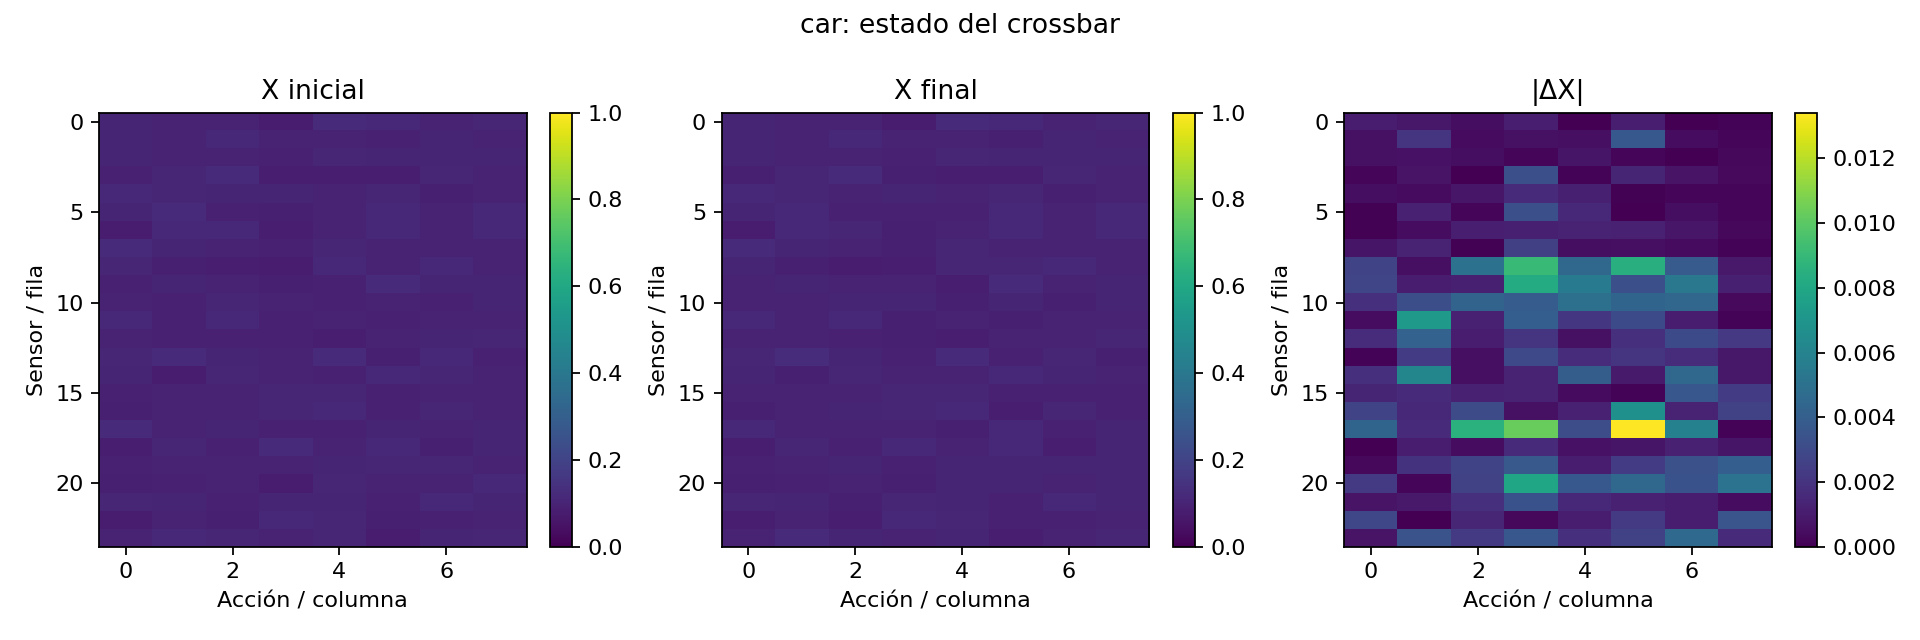
\includegraphics[width=\linewidth,height=0.14\textheight,keepaspectratio]{../../03_EVIDENCIAS/ENTRENAMIENTOS/CAR_RSTDP_EVAL100_SEEDS_2_4_X0/runs/car_rstdp_seed2_X0_0.1/crossbar.png}
\end{minipage}\hfill
\begin{minipage}[t]{0.49\textwidth}
\centering
\textit{Curva de \'exito}\par
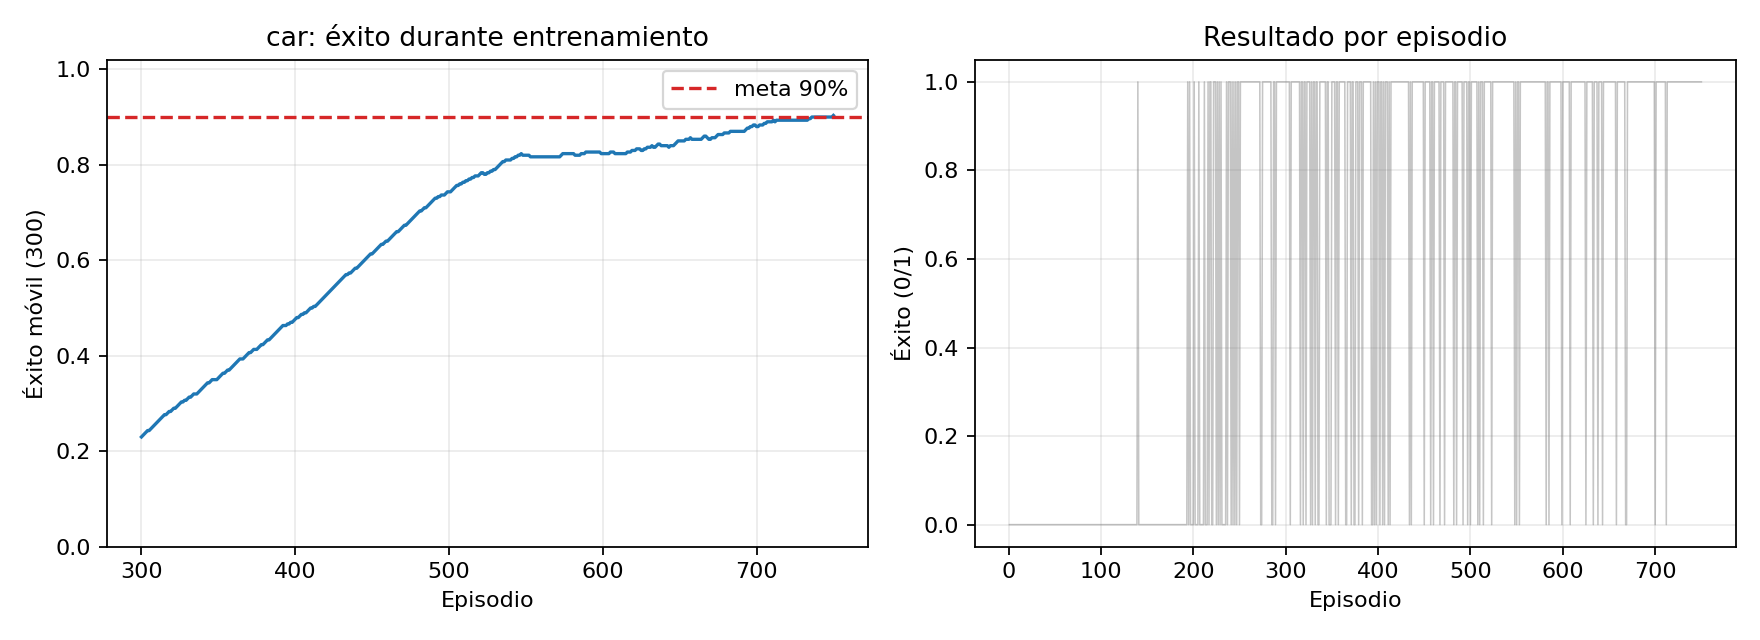
\includegraphics[width=\linewidth,height=0.14\textheight,keepaspectratio]{../../03_EVIDENCIAS/ENTRENAMIENTOS/CAR_RSTDP_EVAL100_SEEDS_2_4_X0/runs/car_rstdp_seed2_X0_0.1/success_curve.png}
\end{minipage}\par\smallskip
\noindent\textbf{Car | R-STDP | semilla 2 | $X_0=0.9$}\\
{\scriptsize Car R-STDP, evaluaci\'on cada 100 episodios; episodios completados: 1548; tasa de \'exito en la ventana final: 90.33\%; criterio alcanzado: s\'i.}\par
\noindent\begin{minipage}[t]{0.49\textwidth}
\centering
\textit{Crossbar $X$}\par
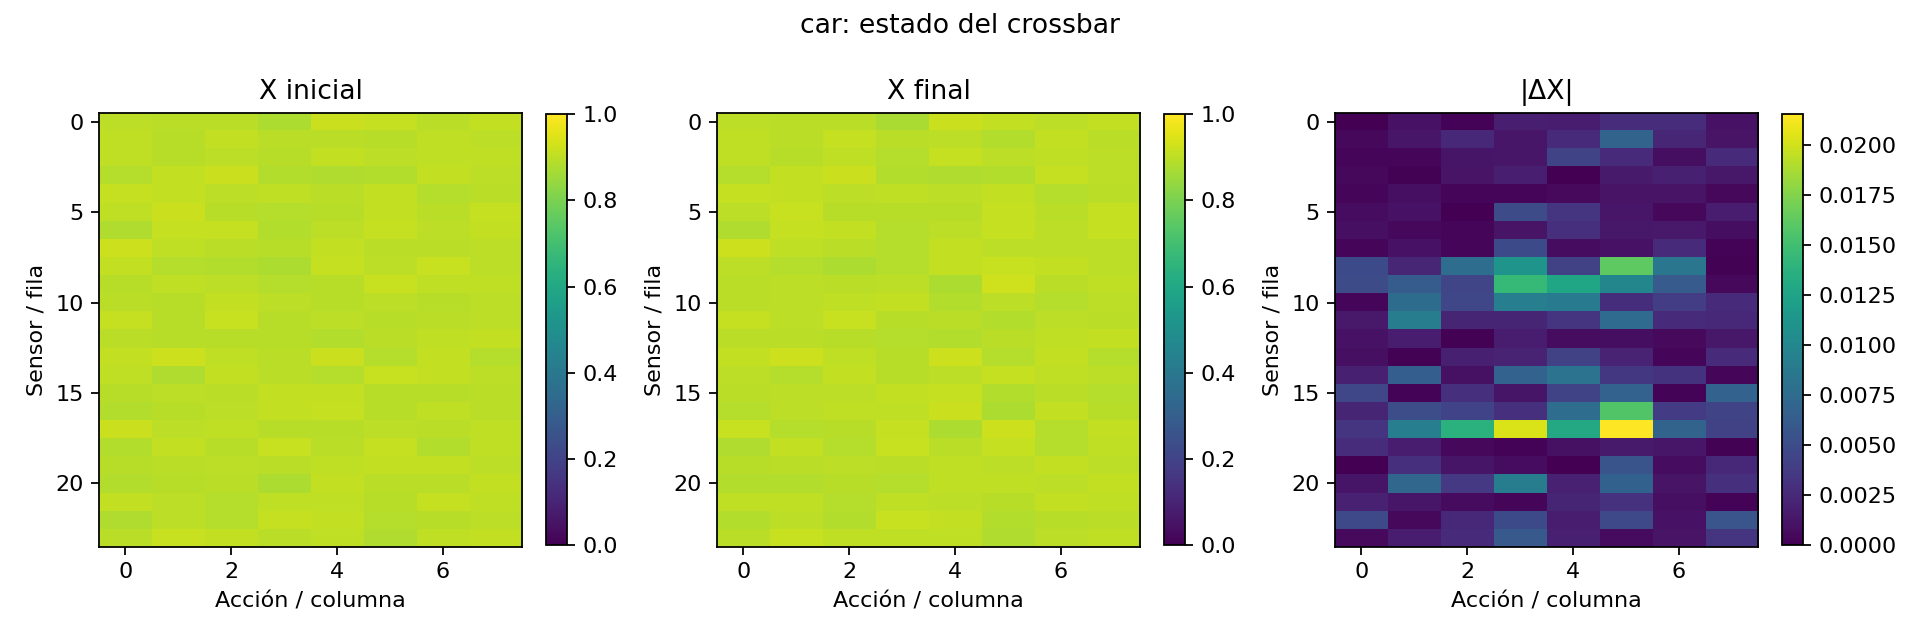
\includegraphics[width=\linewidth,height=0.14\textheight,keepaspectratio]{../../03_EVIDENCIAS/ENTRENAMIENTOS/CAR_RSTDP_EVAL100_SEEDS_2_4_X0/runs/car_rstdp_seed2_X0_0.9/crossbar.png}
\end{minipage}\hfill
\begin{minipage}[t]{0.49\textwidth}
\centering
\textit{Curva de \'exito}\par
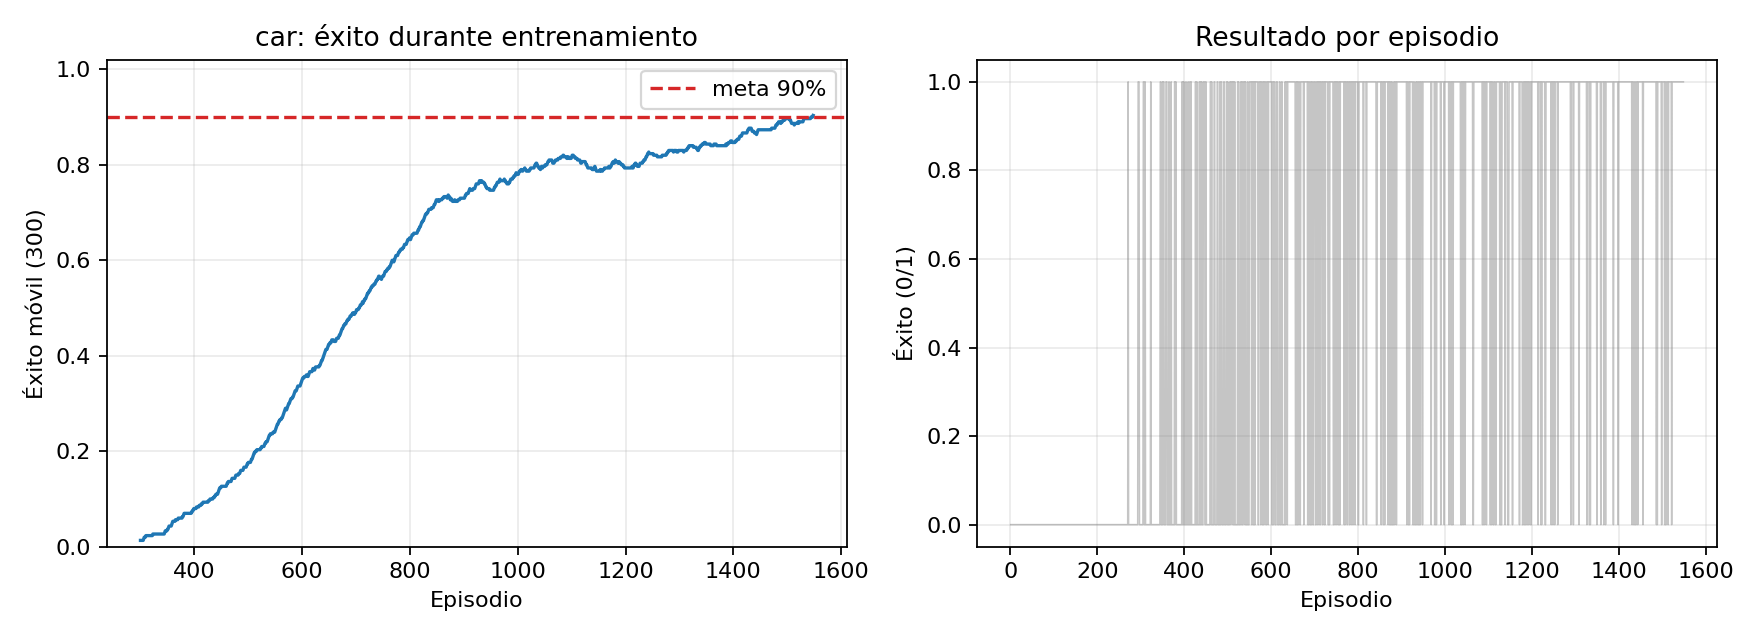
\includegraphics[width=\linewidth,height=0.14\textheight,keepaspectratio]{../../03_EVIDENCIAS/ENTRENAMIENTOS/CAR_RSTDP_EVAL100_SEEDS_2_4_X0/runs/car_rstdp_seed2_X0_0.9/success_curve.png}
\end{minipage}\par\smallskip
\noindent\textbf{Car | R-STDP | semilla 4 | $X_0=0.1$}\\
{\scriptsize Car R-STDP, evaluaci\'on cada 100 episodios; episodios completados: 10000; tasa de \'exito en la ventana final: 8.00\%; criterio alcanzado: no.}\par
\noindent\begin{minipage}[t]{0.49\textwidth}
\centering
\textit{Crossbar $X$}\par
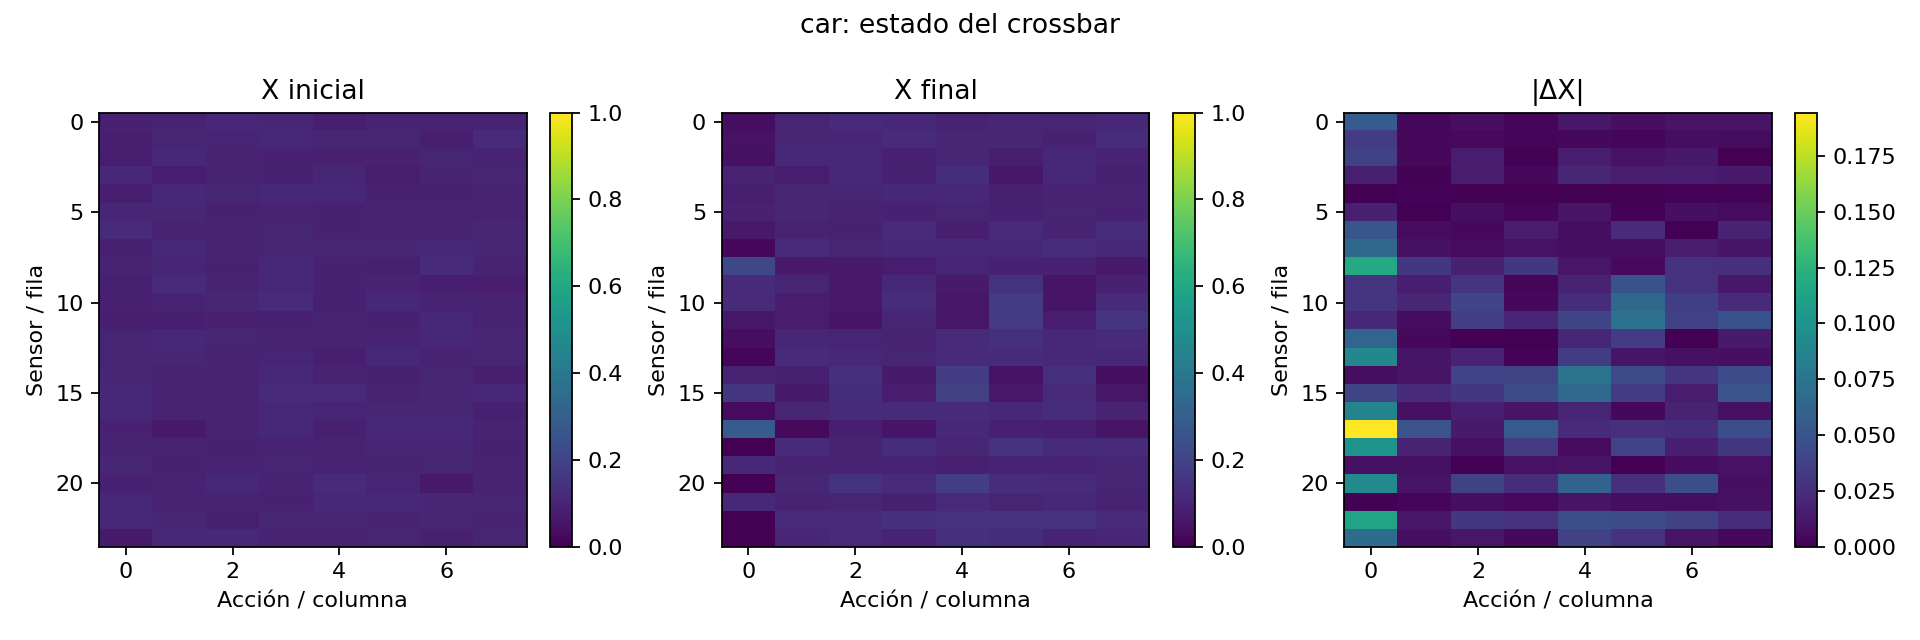
\includegraphics[width=\linewidth,height=0.14\textheight,keepaspectratio]{../../03_EVIDENCIAS/ENTRENAMIENTOS/CAR_RSTDP_EVAL100_SEEDS_2_4_X0/runs/car_rstdp_seed4_X0_0.1/crossbar.png}
\end{minipage}\hfill
\begin{minipage}[t]{0.49\textwidth}
\centering
\textit{Curva de \'exito}\par
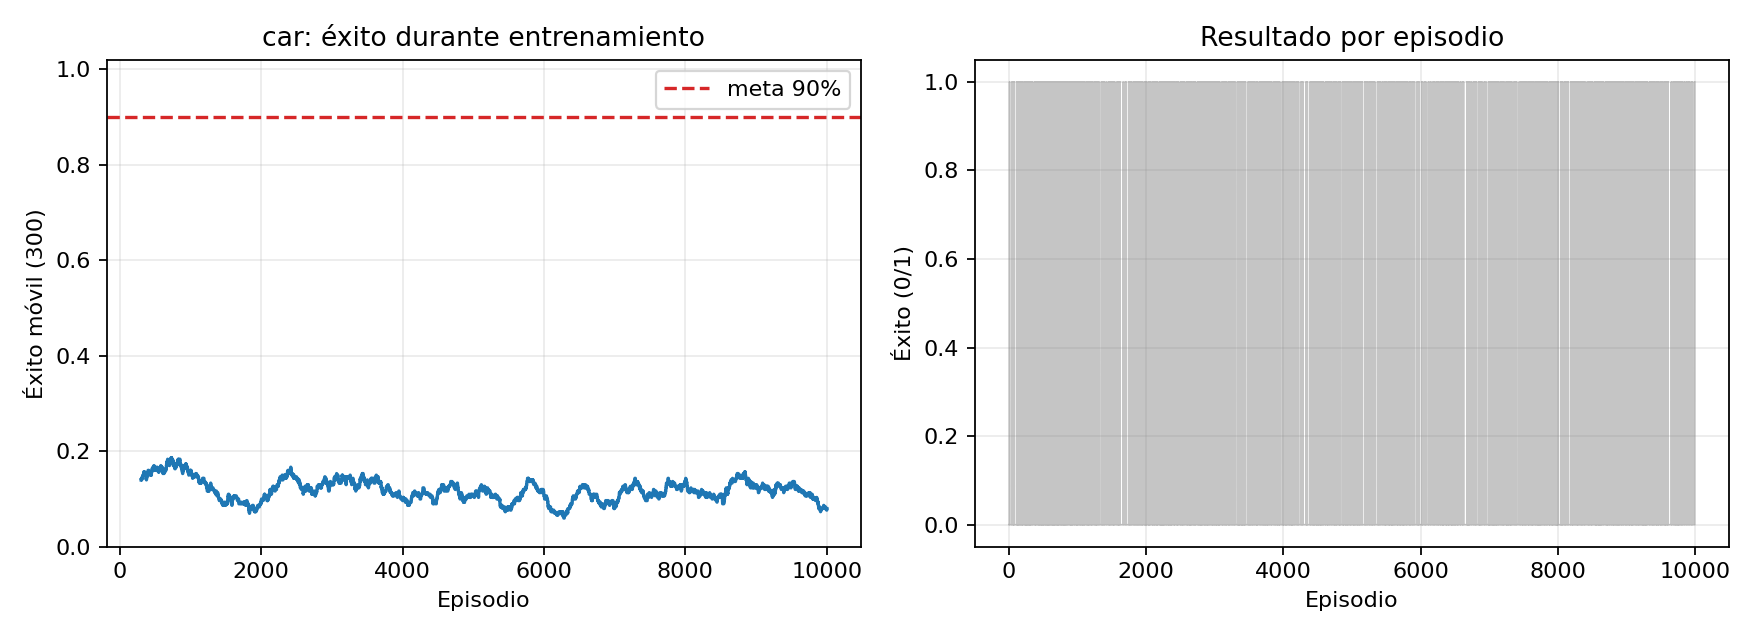
\includegraphics[width=\linewidth,height=0.14\textheight,keepaspectratio]{../../03_EVIDENCIAS/ENTRENAMIENTOS/CAR_RSTDP_EVAL100_SEEDS_2_4_X0/runs/car_rstdp_seed4_X0_0.1/success_curve.png}
\end{minipage}\par\smallskip
\noindent\textbf{Car | R-STDP | semilla 4 | $X_0=0.9$}\\
{\scriptsize Car R-STDP, evaluaci\'on cada 100 episodios; episodios completados: 10000; tasa de \'exito en la ventana final: 10.67\%; criterio alcanzado: no.}\par
\noindent\begin{minipage}[t]{0.49\textwidth}
\centering
\textit{Crossbar $X$}\par
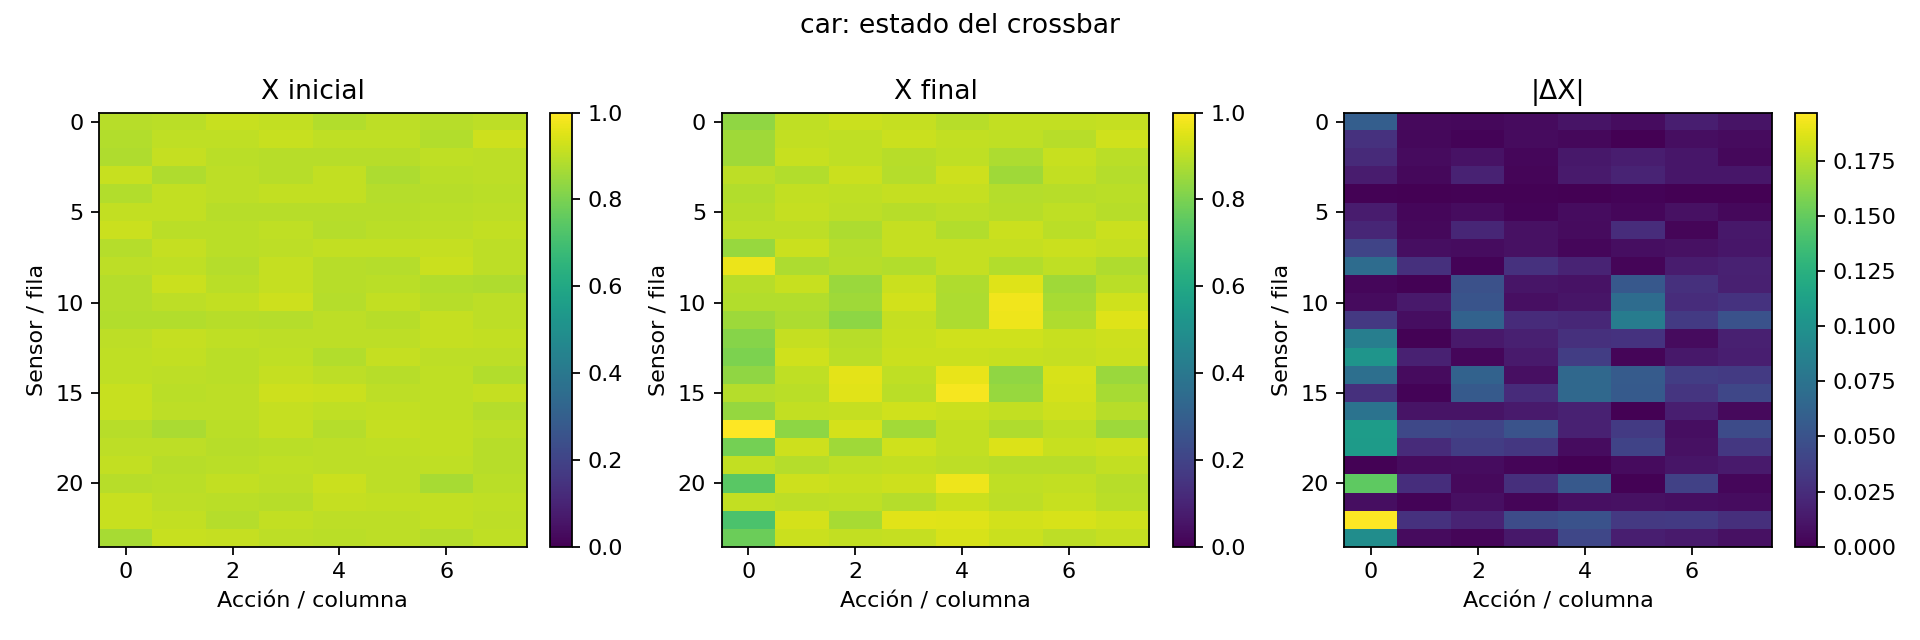
\includegraphics[width=\linewidth,height=0.14\textheight,keepaspectratio]{../../03_EVIDENCIAS/ENTRENAMIENTOS/CAR_RSTDP_EVAL100_SEEDS_2_4_X0/runs/car_rstdp_seed4_X0_0.9/crossbar.png}
\end{minipage}\hfill
\begin{minipage}[t]{0.49\textwidth}
\centering
\textit{Curva de \'exito}\par
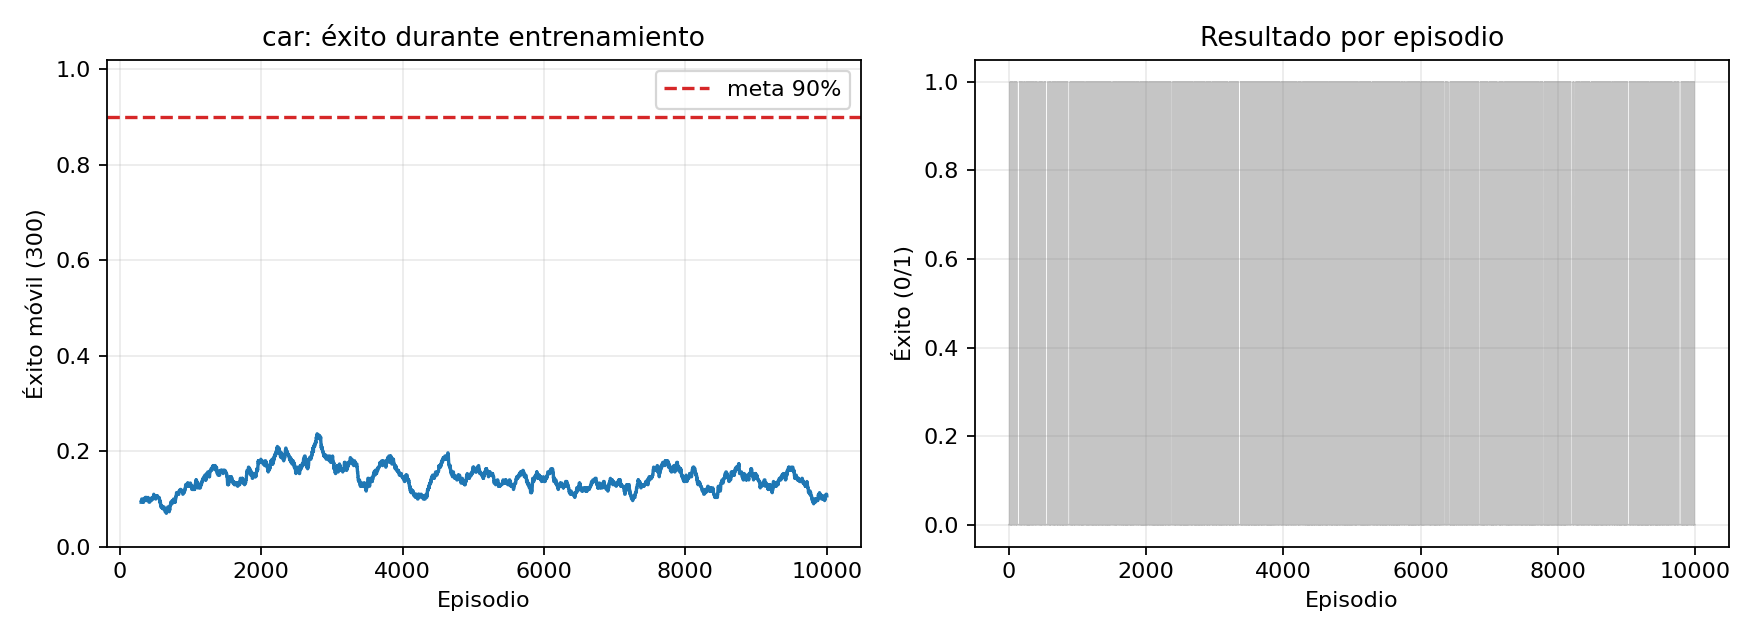
\includegraphics[width=\linewidth,height=0.14\textheight,keepaspectratio]{../../03_EVIDENCIAS/ENTRENAMIENTOS/CAR_RSTDP_EVAL100_SEEDS_2_4_X0/runs/car_rstdp_seed4_X0_0.9/success_curve.png}
\end{minipage}\par\smallskip

\fi

\clearpage
\phantomsection
\addcontentsline{toc}{chapter}{\numberline{}Bibliografía}
% Estilo de bibliografía
\bibliographystyle{IEEEtran}
% Archivo Bibtex para las referencias
\begingroup
\interlinepenalty=10000
\bibliography{references}
\endgroup

\end{document}
